% !Mode:: "TeX:UTF-8"
\documentclass[openleft]{book}
%\usepackage[scheme=chinese,9pt,heading]{ctex}
\usepackage{pifont}
%\usepackage{fontawesome}
\usepackage{fontspec}
\usepackage{amsmath}
\usepackage{amssymb}
\usepackage{bm}
\usepackage{array}
\usepackage{enumitem}
\usepackage{imakeidx}
\usepackage[numbers,sort&compress]{natbib}
\usepackage
[paperheight=26 true cm,paperwidth=18.4 true cm,
top=2.6 true cm,bottom=2.2 true cm,left=2.8 true cm,right=2.8 true cm]
{geometry}
\usepackage{float}
%\usepackage{setspace}
\usepackage{hyperref}
\usepackage{bookmark}
\usepackage{caption}
%\usepackage[perpage,symbol*, bottom,hang,stable,multiple]{footmisc}
\usepackage[clearempty,pagestyles]{titlesec}
\usepackage{titletoc}
\titlecontents{section}[0pt]{\addvspace{2pt}\filright}
{\contentspush{\thecontentslabel\ }}
{}{\titlerule*[8pt]{.}\contentspage}
\usepackage[cmyk,table,hyperref]{xcolor}
\usepackage{tikz}
\usepackage{tcolorbox}
\usepackage{algorithm2e}
\usepackage{listings}
\usepackage{booktabs}
\usepackage{longtable}
\usepackage{makecell}
\usepackage{tabu}
\usepackage{mdframed}
\usepackage{pdfpages}
\usepackage{qrcode}
\usepackage{threeparttable}
%\usepackage{chngcntr}
\usepackage[nottoc,chapter]{tocbibind}
\AtEndPreamble{
	\usepackage[nohyphen,strings]{underscore}
}
\usepackage{lipsum}
%
% .:: footmisc ::.
%
% Circled Digit,带圆圈数字
%\DefineFNsymbols{cd}{{\ding{172}}{\ding{173}}{\ding{174}}{\ding{175}}{\ding{176}}{\ding{177}}{\ding{178}}{\ding{179}}{\ding{180}}{\ding{181}}}
%% Negative Circled Digit,反白带圆圈数字
%\DefineFNsymbols{ncd}{{\ding{182}}{\ding{183}}{\ding{184}}{\ding{185}}{\ding{186}}{\ding{187}}{\ding{188}}{\ding{189}}{\ding{190}}{\ding{191}}}
%% Circled Sans-Serif Digit,带圆圈无衬线数字
%\DefineFNsymbols{cssd}{{\ding{192}}{\ding{193}}{\ding{194}}{\ding{195}}{\ding{196}}{\ding{197}}{\ding{198}}{\ding{199}}{\ding{200}}{\ding{201}}}
%% Negative Circled Sans-Serif Digit,反白带圆圈无衬线数字
%\DefineFNsymbols{ncssd}{{\ding{202}}{\ding{203}}{\ding{204}}{\ding{205}}{\ding{206}}{\ding{207}}{\ding{208}}{\ding{209}}{\ding{210}}{\ding{211}}}
%\setfnsymbol{cssd}
%\setlength\footnotemargin{.6em}

% package: float
\floatplacement{figure}{!ht}

% package: booktab
%\setlength\aboverulesep{0sp}
%\setlength\belowrulesep{0sp}
%\setlength\cmidrulesep{0sp}

% package: graphicx
\graphicspath{{resources/}}

% package: caption
%\DeclareCaptionFont{31104}{\FZYZK}
%\captionsetup{format=hang,labelsep=quad,font=31104}
%\DeclareCaptionFormat{31104}{%
%%	\bfseries\footnotesize#3
%\footnotesize#3
%}
%\captionsetup[lstlisting]{format=31104,singlelinecheck=off}

% package: enumitem
%\setlist{noitemsep,partopsep=0pt}%,listparindent=\parindent
%\setlist[1]{labelindent=\parindent}
%\setlist[itemize]{topsep=0pt,parsep=.5\parskip,leftmargin=1.5em}
%\setlist[itemize]{topsep=0pt,parsep=.5\parskip,leftmargin=3.5em}
%\setlist[enumerate]{topsep=0pt,parsep=.5\parskip,labelsep=*,leftmargin=1.5em}
%\setlist[enumerate,1]{topsep=0pt,parsep=.5\parskip,labelsep=*,leftmargin=3.5em}
%\setlist[description]{topsep=0pt,parsep=.5\parskip,labelsep=.25em,leftmargin=*}

% 图表编号分隔符
\makeatletter
\renewcommand\thefigure{\ifnum \c@chapter>\z@ \thechapter -\fi \@arabic\c@figure}
\renewcommand\thetable{\ifnum \c@chapter>\z@ \thechapter -\fi \@arabic\c@table}
\makeatother

%\setlength{\parskip}{2em}

% 代码风格
\lstset{ %
	language=C++,                % the language of the code
	basicstyle=\scriptsize \fontspec{Monaco},           % the size of the fonts that are used for the code
	numbers=left,                   % where to put the line-numbers
	numberstyle=\tiny\color{gray},  % the style that is used for the line-numbers
%	% will be numbered
	numbersep=5pt,                  % how far the line-numbers are from the code
	showspaces=false,               % show spaces adding particular underscores
	showstringspaces=false,         % underline spaces within strings
%	showtabs=false,                 % show tabs within strings adding particular underscores
	frame=single,                   % adds a frame around the code
%	%	rulecolor=\color{black},        % if not set, the frame-color may be changed on line-breaks within not-black text (e.g. commens (green here))
	tabsize=2,                      % sets default tabsize to 2 spaces
	%	captionpos=b,                   % sets the caption-position to bottom
	breaklines=true,                % sets automatic line breaking
%	breakatwhitespace=false,        % sets if automatic breaks should only happen at whitespace
%	title=\lstname,                   % show the filename of files included with \lstinputlisting;
	% also try caption instead of title
	keywordstyle=\textbf,          % keyword style
}

% 目录双栏
%\usepackage{multicol}
%\makeatletter
%\renewcommand\tableofcontents{%
%	\begin{multicols}{2}[%
%		\section*{%
%			\contentsname
%			\@mkboth{\MakeUppercase\contentsname}{\MakeUppercase\contentsname}}]%
%		\@starttoc{toc}%
%\end{multicols}}
%\makeatother
\makeatletter

\providecommand\optional{\stepcounter{enumi}\labelenumi\makebox[0pt][l]{$^*$}}

% +----------------------------------------------+
% : 重定义                                       :
% +----------------------------------------------+
\renewcommand{\figureautorefname}{\figurename}
\renewcommand{\tableautorefname}{\tablename}


% +----------------------------------------------+
% : 废弃命令                                     :
% +----------------------------------------------+
\def\tightlist{}

% +----------------------------------------------+
% : 取消篇标题单独页                             :
% +----------------------------------------------+
\def\@endpart{}

% +----------------------------------------------+
% : PDF属性设置                                  :
% +----------------------------------------------+
\AtEndPreamble{
	\hypersetup{
		pdfinfo={
			Title    = {\@title},
			Author   = {\@author},
			Creator  = {Adobe Acrobat 11.0},
			Producer = {Acrobat Web Capture 11.0}
		}
	}
}

% +----------------------------------------------+
% : tex.stackexchange.com/a/40363                :
% +----------------------------------------------+
\patchcmd{\@addtocurcol}%
	{\vskip \intextsep}%
	{\edef\save@first@penalty{\the\lastpenalty}\unpenalty
		\ifnum \lastpenalty = \@M % hopefully the OR penalty
			\unpenalty
		\else
			\penalty \save@first@penalty \relax % put it back
		\fi
		\ifnum \outputpenalty <-\@Mii
			\addvspace\intextsep
			\vskip\parskip
		\else
			\addvspace\intextsep
		\fi}%
	{\typeout{*** SUCCESS ***}}{\typeout{*** FAIL ***}}

\patchcmd{\@addtocurcol}%
	{\vskip\intextsep
		\ifnum \outputpenalty <-\@Mii
			\vskip -\parskip
		\fi}%
	{\ifnum \outputpenalty <-\@Mii
		\aftergroup\vskip\aftergroup\intextsep
		\aftergroup\nointerlineskip
	\else
		\vskip\intextsep
	\fi}% was the float seen in vertical mode?
	{\typeout{*** SUCCESS ***}}{\typeout{*** FAIL ***}}

\patchcmd{\@getpen}{\@M}{\@Mi}
	{\typeout{*** SUCCESS ***}}{\typeout{*** FAIL ***}}

% +----------------------------------------------+
% : Verbatim callouts                            :
% +----------------------------------------------+

% Counters for cross-referencing callouts
\newcounter{cocnt}
\newcounter{colref}

% How to represent the <co> markup.
% Big thanks to Jean-Côme Charpentier for his help.
%
\newlength{\co@width}
\newlength{\co@height}
\newlength{\balldiam}
\newlength{\ballcentre}
\newlength{\ballcenter}% 修正纵向位置

\def\conum#1{%
	\sbox{\z@}{\color{white}\sffamily\bfseries\tiny#1}% 
	% Box sizes for any number with two digits
	\sbox{\@ne}{\color{white}\sffamily\bfseries\tiny00}%
	\settowidth{\co@width}{\usebox{\@ne}}%
	\settoheight{\co@height}{\usebox{\@ne}}%
	% Find out the biggest length, to define the circle diameter
	\ifnum\co@width>\co@height
		\setlength{\balldiam}{\co@width}%
	\else
		\setlength{\balldiam}{\co@height}%
	\fi
	\balldiam=1.45\balldiam
	\ballcentre=0.5\balldiam
	\ballcenter=0.3\balldiam% 修正纵向位置
	\setlength{\unitlength}{1pt}% In the case it has been changed
	\begin{picture}(\strip@pt\balldiam,\strip@pt\balldiam) %
	\put(\strip@pt\ballcentre,\strip@pt\ballcenter){\circle*{\strip@pt\balldiam}}
	\put(\strip@pt\ballcentre,\strip@pt\ballcenter){\makebox(0,0){\usebox{\z@}}}
	\end{picture}%
}

% How to represent a <co> embedded in a listing
\def\co#1{\refstepcounter{cocnt}\conum{#1}}

% Make the <co> text and the label to link to
\def\coref#1#2{\co{#1}\label{#2}}

% Make only the <co> label to link to
\def\colabel#1{\refstepcounter{cocnt}\label{#1}}

% Make the <callout> label to link to
\def\collabel#1{\refstepcounter{colref}\label{#1}}

\makeatother


\makeatletter

\setCJKmainfont[BoldFont=方正黑体_GBK,ItalicFont=方正楷体_GBK]{方正书宋_GBK}
\setCJKsansfont[BoldFont=方正黑体_GBK]{方正准圆_GBK}
\setCJKmonofont[BoldFont=方正黑体_GBK]{方正楷体_GBK}
\setmainfont{Times New Roman}
%\setsansfont{Menlo}
\setmonofont{Monaco}
%\setmonofont{Menlo}
\newCJKfontfamily{\FZDBSK}{方正大标宋_GBK}
\newCJKfontfamily{\FZXBSK}{方正小标宋_GBK}
\newCJKfontfamily{\FZHTK}{方正黑体_GBK}
\newCJKfontfamily{\FZKTK}{方正楷体_GBK}
\newCJKfontfamily{\FZFSK}{方正仿宋_GBK}
\newCJKfontfamily{\FZYZK}{方正准圆_GBK}

\makeatother

\newpagestyle{special}[\sffamily\FZHTK\small]{
  \sethead[\thepage][][\chaptertitle]
          {\chaptertitle}{}{\thepage}
}
\newpagestyle{main}[\sffamily\FZHTK\small]{
  \sethead[\thepage][][视觉SLAM十四讲:从理论到实践]
          {\CTEXthechapter\quad\chaptertitle}{}{\thepage}
}

\usepackage{titletoc}
\contentsmargin{1.75em}
\dottedcontents{chapter}[4em]{\bfseries}{4em}{5pt}
\dottedcontents{section}[4em]{}{2.75em}{3pt}
\dottedcontents{subsection}[7em]{\FZKTK}{3em}{3pt}


\setlength{\skip\footins}{5mm}
\setlength\parskip{1pt}

\renewcommand{\arraystretch}{1.2}

\begin{document}
\frontmatter % 开始前言目录,页码用罗马数字
\addtocontents{toc}{\protect\setcounter{tocdepth}{-1}}
\hypersetup{bookmarksdepth=0}
\pdfbookmark[0]{扉页}{titlepage}

\includepdf[noautoscale]{titlepage}
\pagestyle{empty}
\pdfbookmark[0]{版权页}{copyright}
\pagestyle{empty}
{

{\noindent\hfill\bfseries 内\ 容\ 简\ 介\hfill}

本书系统介绍了视觉SLAM(同时定位与地图构建)所需的基本知识与核心算法,既包括数学理论基础,如三维空间的刚体运动、非线性优化,又包括计算机视觉的算法实现,例如多视图几何、回环检测等。此外,我们还提供了大量的实例代码供读者学习研究,从而更深入地掌握这些内容。

本书可以作为对SLAM感兴趣的研究人员的入门自学材料,也可以作为SLAM相关的高校本科生或研究生课程教材使用。

\vspace{\stretch{1}}

未经许可,不得以任何方式复制或抄袭本书之部分或全部内容。

版权所有,侵权必究。

\vspace{\stretch{2}}

\noindent\bfseries 图书在版编目(CIP)数据\normalfont

\noindent{}视觉SLAM十四讲:从理论到实践 / 高翔等著.—北京:电子工业出版社,2017.3\\
ISBN 978-7-121-31104-8\\
\uppercase\expandafter{\romannumeral1}. \ding{172}视… \uppercase\expandafter{\romannumeral2}. \ding{172}高…\uppercase\expandafter{\romannumeral3}. \ding{172}人工智能-视觉跟踪-研究\uppercase\expandafter{\romannumeral4}. \ding{172}TP18

\noindent{}中国版本图书馆CIP数据核字(2017)第053910号

\vspace{\stretch{2}}

\noindent 策划编辑:郑柳洁\\
责任编辑:白 涛\\
印  刷:北京季蜂印刷有限公司\\
装  订:北京季蜂印刷有限公司\\
出版发行:电子工业出版社\\
     北京市海淀区万寿路173信箱   邮编:100036\\
开  本:720×1000 1/16  印张:25  字数:560千字\\
版  次:2017年3月第1版\\
印  次:2018年1月第7次印刷\\
定  价:75.00元

\vspace{\stretch{1}}

凡所购买电子工业出版社图书有缺损问题,请向购买书店调换。若书店售缺,请与本社发行部联系,联系及邮购电话:(010)88254888,88258888。

质量投诉请发邮件至zlts@phei.com.cn,盗版侵权举报请发邮件至dbqq@phei.com.cn。

本书咨询联系方式:(010)51260888-819\quad faq@phei.com.cn。
}

\pagestyle{special}

% 读者须知
\chapter{阅读须知}

\section*{本书图片}

为描述方便,书中介绍图片相关内容时直接使用了对应的色彩名称,对应到纸面上即灰色。此外,部分图片可能需要放大观察,纸面上无法呈现应有效果。为此,书中图片均在博文视点官方网站提供下载。

\section*{读者服务}

轻松注册成为博文视点社区用户(www.broadview.com.cn{}),您即可享受以下服务。

\begin{itemize}
\item \textbf{下载资源:}本书所提供的示例代码及资源文件均可在 \underline{\emph{下载资源}}处下载。

\item \textbf{提交勘误:}您对书中内容的修改意见可在 \underline{\emph{提交勘误}}处提交,若被采纳,将获赠博文视点社区积分(在您购买电子书时,积分可用来抵扣相应金额)。

\item \textbf{与作者交流:}在页面下方 \underline{\emph{读者评论}}处留下您的疑问或观点,与作者和其他读者一同学习交流。
\end{itemize}

页面入口:\url{http://www.broadview.com.cn/31104}

\begin{centering}
\begin{tikzpicture}[baseline={([yshift={-8pt}]current bounding box.north)},outer sep=0pt,inner sep=0pt]
\node[label={[inner sep=1pt,fill=white]center:{\includegraphics[height=20pt]{31104-fm.jpg}}}]{\qrcode*[height=3cm,level=H]{http://www.broadview.com.cn/31104}};
\end{tikzpicture}
\end{centering}


% 版权
\pdfbookmark[0]{\contentsname}{copyright}

% 第二版序言
\thispagestyle{empty}
\chapter*{第二版序}
自《视觉SLAM十四讲:从理论到实践》出版以来已经过去了一年多的时间。这一年内,这本书在业界引起了广泛的关注和讨论。大多数读者评价是正面的,不过也有些地方不够令人满意。比如说,这本书作为初学者向,入门则入门矣,有些应该深入的地方还讲得不够深入;再比如说,书的数学符号不够统一,有些地方容易令读者产生了误解。还有的地方,读者认为叙述不够有趣,我没有完全放开,这都是事实,所以我准备在第二版中更加放飞自我一些。

实际上,第一版书是在2016年中期开始写的,所有文字、图片和代码都需要从头准备,再加上我也是第一次写这么厚的书,错误部分所在难免。2018年,我在慕尼黑工大给学生讲SLAM课程,期间又积累了一些材料。所以第二版书从内容上也会更丰富,更合理一些。第二版在第一版的基础上做的改动有:
\begin{enumerate}
\item 更多的实例。我增加了一些实验代码来介绍算法的原理。在第一版中,多数实践代码调用了各种库中的内置函数,我现在认为更加深入地介绍底层计算会更好一些。所以第二版的许多代码,在调用库函数之外,还提供了底层的实现。
\item 更深入的内容,特别是第七章至第十二章,同时也删除了一些泛泛而谈的边角料。对第一版大部分数学公式进行了审视,重写了那些容易引起误解的地方。
\item 更完善的项目。我将第一版的第九章移至了第十三章。于是,我们可以在介绍了所有必要知识之后,向大家展现一个完整的SLAM系统如何工作了。
\item 更通俗、简洁、口语化的表达,我觉得这是一本好书的标准,特别是介绍一些看起来高深莫测的数学知识时。我也重新制作了部分插图,在黑白打印成书之后会看起来更清楚一些。
\item 当然,每章前的简笔画我是不会改的!
\end{enumerate}

总之,我尽量做到深入浅出,也希望第二版书能够给你更加舒适的阅读体验。

\clearpage

\tableofcontents % 目录

\mainmatter % 开始正文,页码用阿拉伯数字
\pagestyle{main}
\addtocontents{toc}{\protect\setcounter{tocdepth}{2}}
\hypersetup{bookmarksdepth=2}

%%%%%%%%%%%%%%%%%%%%%%%%%%%%%%%%%%

% ch1 前言
% 这章最好是“第零章”或者在序言里
\chapter{预备知识}
\section{本书讲什么}

这是一本介绍视觉SLAM的书,也很可能是第一本以视觉SLAM为主题的中文书。

那么,SLAM是什么?

SLAM是\textbf{S}imultaneous \textbf{L}ocalization \textbf{a}nd \textbf{M}apping的缩写,中文译作“\textbf{同时定位与地图构建}”\textsuperscript{\cite{Liu2016}}。它是指搭载特定\textbf{传感器}的主体,在\textbf{没有环境先验信息}的情况下,于\textbf{运动过程中}建立\textbf{环境}的模型,同时估计自己的\textbf{运动}\textsuperscript{\cite{Davison2007}}。如果这里的传感器主要为相机,那就称为“视觉SLAM”。

本书的主题就是视觉SLAM。这里我们刻意把许多个定义放到一句话中,希望帮助读者建立一个较明确的概念。首先,SLAM的目的是解决“定位”与“地图构建”这两个问题。也就是说,一边要估计传感器自身的位置,一边要建立周围环境的模型。那么怎么解决呢?这需要用到传感器的信息。传感器以一定形式观察外部世界,但不同传感器观察的方式是不同的。之所以要花一本书的内容去讨论这个问题,是因为它很难——特别是我们希望\textbf{实时地}、在\textbf{没有先验知识}的情况下进行SLAM。当用相机作为传感器时,我们要做的就是根据一张张连续运动的图像(它们形成了一段视频),从中推断相机的运动,以及周围环境的情况。

这似乎是个很直观的问题。我们自己走进陌生的环境时不就是这么做的吗?

在计算机视觉(Computer Vision)创立之初,人们就想象着有朝一日,计算机将和人一样,通过眼睛去观察世界,理解周遭的物体,探索未知的领域——这是一个美妙而又浪漫的梦想,吸引了无数的科研人员日夜为之奋斗\textsuperscript{\cite{Hartley2003}}。我们曾经以为这件事情并不困难,然而进展却远不如预想的那么顺利。我们眼中的花草树木、虫鱼鸟兽,在计算机中却是那样的不同:它们只是一个个由数字排列而成的矩阵。让计算机理解图像的内容,就像让我们自己理解这些数字一样困难。我们既不了解自己如何理解图像,也不知道计算机该如何理解、探索这个世界。于是我们困惑了很久,直到几十年后的今天,才发现了一点点成功的迹象:通过人工智能(Artificial Intelligence)中的机器学习(Machine Learning)技术,计算机渐渐能够辨别出物体、人脸、声音、文字——尽管它所用的方式(统计建模)与我们是如此不同。另一方面,在SLAM发展了将近30年之后,我们的相机才渐渐开始能够认识到自身的位置,发觉自己在运动——虽然方式还是和人类有巨大的差异。不过,至少研究者们已经成功地搭建出种种实时SLAM系统,有的能够快速跟踪自身位置,有的甚至能够进行实时的三维重建。

这件事情确实很困难,但我们已经有了很大的进展。更令人兴奋的是,近年来随着科技的发展,涌现出了一大批与SLAM相关的应用点。在许多地方,我们都希望知道自身的位置:室内的扫地机和移动机器人需要定位,野外的自动驾驶汽车需要定位,空中的无人机需要定位,虚拟现实和增强现实的设备也需要定位。SLAM是那样重要。没有它,扫地机就无法在房间自主地移动,只能盲目地游荡;家用机器人就无法按照指令准确到达某个房间;虚拟现实也将永远固定在座椅之上\footnote{目前虚拟现实头盔普遍只追踪原地旋转运动,而无法追踪更大范围内的平移运动。}——所有这些新奇的事物都无法出现在现实生活中,那将多么令人遗憾。

今天的研究者和应用开发人员,逐渐意识到了SLAM技术的重要性。在国际上,SLAM已经有近三十年的研究历史,也一直是机器人和计算机视觉的研究热点。21世纪以来,以视觉传感器为中心的\textbf{视觉SLAM技术},在理论和实践上都经历了明显的转变与突破,正逐步从实验室研究迈向市场应用。同时,我们又遗憾地发现,至少在国内,与SLAM相关的论文、书籍仍然非常匮乏,让许多对SLAM技术感兴趣的初学者无从一窥门径。虽然SLAM的理论框架基本趋于稳定,但其编程实现仍然较为复杂,有着较高的技术门槛。刚步入SLAM领域的研究者,不得不花很长的时间,学习大量的知识,往往要走过许多弯路才得以接近SLAM技术的核心。

本书全面系统地介绍了以视觉传感器为主体的视觉SLAM技术,我们希望它能(部分地)填补这方面资料的空白。我们会详细地介绍SLAM的理论背景、系统架构,以及各个模块的主流做法。同时,\textbf{极其重视实践}:本书介绍的\textbf{所有}重要算法,都将给出可以运行的实际代码,以求加深读者的理解。在第二版中,我们对于大多数算法,会讨论内在的原理,而非简单地从函数库中进行调用。之所以这么做,主要是考虑到SLAM毕竟是一项和实践紧密相关的技术。再漂亮的数学理论,如果不能转化为可以运行的代码,那就仍是可望而不可即的空中楼阁,没有实际意义。我们相信,实践出真知,实践出真爱。只有实际地演算过各种算法之后,你才能真正地认识SLAM,真正地喜欢上科研。

自1986年提出以来\textsuperscript{\cite{Smith1986}},SLAM一直是机器人领域的热点问题。关于它的文献数以千计,想要对SLAM发展史上的所有算法及变种做一个完整的说明,是十分困难而且没有必要的。本书中会介绍SLAM所牵涉的背景知识,例如射影几何、计算机视觉、状态估计理论、李群李代数等,并在这些背景知识之上,给出SLAM这棵大树的主干,而略去一部分形状奇特、纹理复杂的枝叶。我们认为这种做法是有效的。如果读者能够掌握主干的精髓,那么自然会有能力去探索那些边缘的、细节的、错综复杂的前沿知识。所以,我们的目的是,让SLAM的初学者通过阅读本书快速地成长为能够探索这个领域边缘的研究者。另一方面,即便你已经是SLAM领域的研究人员,本书也可能有一些你还觉得陌生的地方,可以让你产生新的见解。

目前,与SLAM相关的书籍主要有《概率机器人》(\textit{Probabilistic robotics})\textsuperscript{\cite{Thrun2005}}、《计算机视觉中的多视图几何》(\textit{Multiple View Geometry in Computer Vision})\textsuperscript{\cite{Hartley2003}}、《机器人学中的状态估计》(\textit{State Estimation for Robotics: A Matrix-Lie-Group Approach})\textsuperscript{\cite{Barfoot2016}}\footnote{已有中文版,我也参与了翻译。}等。它们内容丰富、论述全面、推导严谨,是SLAM研究者中脍炙人口的经典教材。然而就目前来看,还存在两个重要的问题:其一,这些图书的目的在于介绍基础理论,SLAM只是其应用之一。因此,它们并不能算是专门讲解SLAM的书籍。其二,它们的内容偏重于数学理论,基本不涉及编程实现,导致读者经常出现“书能看懂却不会编程”的情况。而我们认为,只有读者亲自实现了算法,调试了各个参数,才能谈得上真正理解了问题本身。

我们会提及SLAM的历史、理论、算法、现状,并把完整的SLAM系统分成几个模块:视觉里程计、后端优化、建图,以及回环检测。我们将陪着读者一点点实现这些模块中的核心部分,探讨它们在什么情况下有效,什么情况下会出问题,并指导大家在自己的机器上运行这些代码。你会接触到一些\textbf{必要的}数学理论和许多编程知识,会用到Eigen、OpenCV、PCL、g2o、Ceres等库\footnote{如果你完全没有听说过它们,那么应该感到兴奋,这说明你会从本书中收获很多知识。},掌握它们在Linux操作系统中的使用方法。

从写作风格上,我们不想把本书写成枯燥的理论书籍。技术类图书应该是严谨可靠的,但严谨不意味着刻板。一本优秀的技术书应该是生动有趣而易于理解的。如果你觉得“这个作者怎么这么不正经”,敬请原谅,因为我并不是一个非常严肃的人\footnote{你会经常在脚注中发现一些神奇的东西。}。无论如何,有一件事是可以肯定的:只要你对这门新技术感兴趣,在学习本书的过程中肯定会有所收获!您会掌握与SLAM相关的理论知识,你的编程能力也将有明显的进步。在很多时候,您会有一种“我在陪你一起做科研”的感觉,这正是我所希望的。但愿您能在此过程中发现研究的乐趣,喜欢这种“通过一番努力,看到事情顺利运行”的成就感。

好了,话不多说,祝你旅行愉快!

\section{如何使用本书}
\subsection{组织方式}
本书名为“视觉SLAM十四讲”。顾名思义,我们会像在学校里讲课那样,以“讲”作为本书的基本单元。每一讲都对应一个固定的主题,其中会穿插“理论部分”和“实践部分”两种内容。通常是理论部分在前,实践部分在后。在理论部分中,我们将介绍\textbf{理解算法所必需}的数学知识,并且大多数时候以叙述的方式,而不是像数学教科书那样用“定义—定理—推论”的方式,因为我们觉得这样的方式阅读起来更容易一些,尽管有时候显得不那么严谨。实践部分主要是编程实现,讨论程序里各部分的含义及实验结果。看到标题中带有“实践”两个字的章节,你就应该(兴致勃勃地)打开电脑,和我们一起愉快地编写代码了。

值得一提的是,我们只会把与解决问题相关的数学知识放在书里,并尽量保持浅显。因为我是工科生,所以要勇敢地承认,某些做法只要经验上够用,没必要非得在数学上追求完备。只要我们知道这些算法在绝大多数实际场景下能够工作,并且数学家们(通过冗长而且复杂的证明和讨论)说明在什么情况下可能不工作,那么我就表示满意,而不刻意追究那些看似完美的证明(当然它们固有自己不可否认的价值)。由于SLAM牵涉到了太多数学背景,为了防止使本书变成数学教科书,我们把一些细节上的推导和证明留作习题和补充阅读材料,方便感兴趣的读者进一步阅读参考文献,更深入地掌握相关细节。

每一讲正文之后,我们设计了一些习题。其中,带$^*$号的习题是具有一定难度的。我们强烈建议读者把习题都练习一遍,这对你掌握这些知识很有帮助\footnote{它们也可能成为今后相关行业的面试题,或许还能帮你在找工作时留个好印象。}。

全书内容主要分为两个部分。
\begin{enumerate}
\item 第一部分为\textbf{数学基础}篇,我们会以浅显易懂的方式,铺垫与视觉SLAM相关的数学知识,包括:

\begin{itemize}[leftmargin=1.5em]
	\item 第1讲是前言,介绍这本书的基本信息,习题部分主要包括一些自测题。
	\item 第2讲为SLAM系统概述,介绍一个SLAM系统由哪些模块组成,各模块的具体工作是什么。实践部分介绍编程环境的搭建过程以及IDE的使用。
	\item 第3讲介绍三维空间运动,你将接触到旋转矩阵、四元数、欧拉角的相关知识,并且在Eigen当中使用它们。
	\item 第4讲为李群和李代数。即便你现在不懂李代数为何物,也没有关系。你将学到李代数的定义和使用方式,然后通过Sophus操作它们。
	\item 第5讲介绍针孔相机模型以及图像在计算机中的表达。你将用OpenCV来调取相机的内外参数。
	\item 第6讲介绍非线性优化,包括状态估计理论基础、最小二乘问题、梯度下降方法。你会完成一个使用Ceres和g2o进行曲线拟合的实验。
\end{itemize}

这些就是我们要用到的所有数学知识了,当然,其中还隐含了你以前学过的高等数学和线性代数。我保证它们看起来都不会很难,至少没有听上去那么难。当然,若你想进一步深入挖掘,我们会提供一些参考资料供你阅读,那些材料可能会比正文里讲的知识难一些。

%\clearpage
\item 第二部分为\textbf{SLAM技术}篇。我们会使用第一部分所介绍的理论,讲述视觉SLAM中各个模块的工作原理。

\begin{itemize}[leftmargin=1.5em]
	\item 第7讲为特征点法的视觉里程计。该讲内容比较多,包括特征点的提取与匹配、对极几何约束的计算、PnP和ICP等。在实践中,你将用这些方法去估计两个图像之间的运动。
	\item 第8讲为直接法的视觉里程计。你将学习光流和直接法的原理,然后实现一个简单的直接法运动估计。
	\item 第9讲为后端优化,主要为对Bundle Adjustment的深入讨论,包括基本的BA,以及如何利用稀疏性加速求解过程。你将用Ceres和g2o分别书写一个BA程序。
	\item 第10讲主要讲后端优化中的位姿图。位姿图是表达关键帧之间约束的一种更紧凑的形式。我们会介绍SE(3)和Sim(3)的位姿图,同时你将使用g2o对一个位姿球进行优化。
	\item 第11讲为回环检测,主要介绍以词袋方法为主的回环检测。你将使用dbow3书写字典训练程序和回环检测程序。
	\item 第12讲为地图构建。我们会讨论如何使用单目进行稠密深度图的估计(以及这是多么不可靠),然后讨论RGB-D的稠密地图构建过程。你会书写极线搜索与块匹配的程序,然后在RGB-D中遇到点云地图和八叉树地图的构建问题。
	\item 第13讲是工程章,你将搭建一个双目视觉里程计框架,综合运用先前学过的知识,实现它的基本功能。这个过程中,你会碰到一些问题,例如优化的必要性、关键帧的选择等。我们会在Kitti数据集上测试它的性能,讨论一些改进的手段。
	\item 第14讲主要介绍当前的开源SLAM项目以及未来的发展方向。相信在阅读了前面的知识之后,你会更容易理解它们的原理,实现自己的新想法。
\end{itemize}
\end{enumerate}

最后,如果你完全看不懂上面在说什么,那么恭喜你!这本书很适合你!加油!

\subsection{代码}
本书所有源代码均托管在GitHub上:

{\hfill\url{https://github.com/gaoxiang12/slambook2}\hfill}

\textbf{注意后面有一个2,表示这是第二版书的代码}。我强烈建议读者下载代码以供随时查看。代码是按章节划分的,比如,第7讲的内容就会放在ch7文件夹中。此外,对于书中用到的一些小型库,会以压缩包的形式放在3rdparty文件夹下。在第二版中,我们用git submodule工具来保证读者使用的软件 版本与书中的完全一致,所以读者不必操心软件版本问题。对于像OpenCV那种大中型库,我们会在它们第一次出现时介绍其安装方法。如果你对代码有任何疑问,请单击GitHub上的Issues按钮,提交问题。如果确实是代码出现问题,我们会及时进行修改;即使是你的理解有偏差,我也会尽可能回复。如果你不习惯使用Git,那么单击右侧包含download字样的按钮将代码下载至本地即可。%网上能搜索到很多关于git和github的使用教程。

\subsection{面向的读者}
本书面向对SLAM感兴趣的学生和研究人员。阅读本书需要一定的基础,我们假设你具备以下知识:

\begin{itemize}
\item {\textbf{高等数学、线性代数、概率论}。} 这些是大部分读者应该在大学本科阶段接触过的基本数学知识\footnote{实际当中每个人都至少需要学三遍线性代数:本科一遍,研究生一遍,工作时期一遍。}。你应当明白矩阵和向量是什么,或者做微分和积分是什么意思。对于SLAM中用到的专业知识,我们会额外加以介绍。

\item {\textbf{C++语言基础}。} 由于我们采用C++作为编码语言,所以建议读者至少熟悉这门语言的语法。比如,你应该知道类是什么,如何使用C++标准库,模板类如何使用,等等。我们会避免过多地使用技巧,但有些地方确实无法避免。此外,我们还使用了一些C++ 11标准的内容,不过,我们会在用到的地方加以解释。

\item {\textbf{Linux基础}。} 我们的开发环境是Linux而非Windows,并且只提供Linux下的源程序,\textbf{不会}再提供Windows下的开发方法介绍。\textbf{我们认为,掌握Linux是一个SLAM研究人员所必需的,请初学者暂时不要问为什么,把本书的知识学好之后相信你会和我们有同样的想法。}各种程序库在Linux下的配置都非常便捷,你也会在此过程中体会到Linux的便利。如果读者此前从未使用过Linux,那么最好找一本Linux的教材稍加学习(掌握基本知识即可,一般就是相关图书的前面几章内容)。我们不要求读者具备多么高超的Linux操作技能,但希望读者至少知道“打开终端,进入代码目录”是如何操作的。本讲的习题里有一些Linux知识自测题,如果你清楚自测题的答案,那么阅读本书代码不会有任何问题。
\end{itemize}

对SLAM感兴趣但不具备上述知识的读者,可能在阅读本书时会感到困难。如果你不了解C++的基本知识,可以读一点\emph{C++ Primer Plus}之类的图书入门;如果你缺少相关的数学知识,也可以先阅读一些相关数学教材补充知识,不过我们认为,对大多数大学本科水平的朋友,读懂本书所需的数学背景肯定是具备了。代码方面,你最好花点时间亲自输入一遍,再调节里面的参数,看看效果会发生怎样的改变。这会对学习很有帮助。

本书可作为SLAM相关课程的教材,亦可作为课外自学材料使用。

\section{风格约定}
本书既有数学理论介绍,也有编程实现,因此,为方便阅读,对不同内容采用了不同排版方式加以区分。
\begin{enumerate}
\item 数学公式单独列出,重要的公式还在右侧标了序号,例如:
\begin{equation}
 \bm{y} =\bm{A}\bm{x}.
\end{equation}
数学字体采用国标风格。标量使用斜体字(如$a,\alpha$),向量和矩阵使用粗斜体(如$\bm{a}, \bm{A},\boldsymbol{\Sigma}$,希腊字母除外)。空心粗体代表特殊集合,如实数集$\mathbb{R}$、整数集$\mathbb{Z}$。李代数部分使用哥特体,如$\mathfrak{so}(3),\mathfrak{se}(3)$。
\item 程序代码以方框框出,使用不同的字体和小一些的字号,左侧带有行号。如果程序较长,方框会延续到下一页。总之,看起来像这样:
\begin{lstlisting}[language=C++,caption=示例代码]
#include <iostream>
using namespace std;

int main ( int argc, char** argv )
{
	cout<<"Hello"<<endl;
	return 0;
}
\end{lstlisting}

\item 当代码数量较多或有的部分与之前列出的重复,不适合完全列在书中时,我们会\textbf{仅给出重要片段},并以“片段”二字注明。因此,再说一遍,我们强烈建议读者到GitHub上下载所有源代码,完成练习,以更好地掌握本书知识。

\item 由于排版原因,书中展示的代码可能与GitHub中的代码有稍许不同,请以GitHub上的代码为准。

\item 我们用到的每个库,在第一次出现的时候会有比较详细的安装和使用说明,但在后续的使用中则不再赘述。所以,建议读者按章节顺序阅读本书内容。

\item 每一讲的开头会列出本讲的内容提要,而末尾会有小结和练习题。引用的参考文献在全书末尾列出。

\item 以星号开头的章节是选读部分,读者可以根据兴趣阅读。跳过它们不会对理解后续章节产生影响。

\item 文中重要的内容以\textbf{黑体}标出,相信你已经习惯了。

\item 我们设计的实验大多数是演示性质的。看懂了它们不代表你已经熟悉整个库的使用。所以我们建议你在课外花一点时间,对本书经常用的几个库进行深入学习。

\item 本书的习题和选读内容可能需要你自己搜索额外材料,所以你需要学会使用搜索引擎。
\end{enumerate}

\section{致谢和声明}
在本书漫长的写作过程中,我得到了许多人的帮助,包括但不限于:

\begin{itemize}
	\item 中科院的贺一家博士为第5讲的相机模型部分提供了材料。
	\item 颜沁睿提供了第7讲的公式推导材料。
	\item 华中科大的刘毅博士为本书第6讲和第10讲提供了材料。
	\item 众多的老师、同学为本书提供了修改意见:肖锡臻、谢晓佳、张明明、耿欣、李帅杰、刘富强、袁梦、孙志明、陈昊升、王京、朱晏辰、丁文东、范帝楷、衡昱帆、高扬、李少朋、吴博、闫雪娇、张腾、郑帆、卢美奇、杨楠等等。在此向他们表示感谢。
\end{itemize}

此外,感谢我的导师张涛教授一直以来对我的支持和帮助。感谢电子工业出版社郑柳洁编辑的支持。没有他们的帮助,本书不可能以现在的面貌来到读者面前。本书的成书与出版是所有人共同努力的结晶,尽管我没法把他们都列在作者列表中,但是它的出版离不开他们的工作。\footnote{文章中的“我”主要是指本人高翔,前面说“我”不正经不包括上述其他作者。他们都是敬业乐群的好同志。}

本书写作过程中参考了大量文献和论文。其中大部分数学理论知识是前人研究的成果,并非我的原创。一小部分实验设计亦来自各开源代码的演示程序,不过大部分是我自己编写的。此外,也有一些图片摘自公开发表的期刊或会议论文,文中均已注明。未做说明的图像,或为原创,或来自网络,恕不一一列举。如有问题,请与我们联系,我们会在第一时间加以修正。

本书涉及知识点众多,错漏在所难免。如有疑问,欢迎通过电子邮件与我联系。

我的邮箱是:\href{mailto:gao.xiang.thu@gmail.com}{gao.xiang.thu@gmail.com}。

感谢我的爱人刘丽莲女士长期的理解和支持。这本书是献给她的。

\section*{习题(基本知识自测题)}
\begin{enumerate}
	\item 有线性方程$\bm{A} \bm{x} = \bm{b}$,若已知$\bm{A}, \bm{b}$,需要求解$\bm{x}$,该如何求解?这对$\bm{A}$和$\bm{b}$有哪些要求?提示:从$\bm{A}$的维度和秩角度来分析。
	\item 高斯分布是什么?它的一维形式是什么样子?它的高维形式是什么样子?
	\item 你知道C++中的\textbf{类}吗?你知道STL吗?你使用过它们吗?
	\item 你以前怎样书写C++程序?(你完全可以说只在Visual C++ 6.0下写过C++工程,只要你有写C++和C语言的经验就行。)
	\item 你知道C++11标准吗?其中哪些新特性你听说过或用过?有没有其他的标准?
	\item 你知道Linux吗?你有没有至少使用过一种(不算安卓),比如Ubuntu?
	\item Linux的目录结构是什么样的?你知道哪些基本命令,比如ls, cat等?
	\item 如何在Ubuntu中安装软件(不打开软件中心的情况下)?这些软件被安装在什么地方?如果只知道模糊的软件名称(比如想要装一个名称中含有eigen的库),应该如何安装它?
	\item[\optional] 花一个小时学习一下Vim,因为你迟早会用它。你可以在终端中输入vimtutor阅读一遍所有内容。我们不需要你非常熟练地操作它,只要能够在学习本书的过程中使用它输入代码即可。\textbf{不要在它的插件上浪费时间,不要想着把Vim用成IDE,我们只用它做文本编辑的工作。}
\end{enumerate}
\thispagestyle{empty}
\part{数学基础}
\thispagestyle{empty}
% ch2 概述
% !Mode:: "TeX:UTF-8"
% 第二版:增加clion的一些介绍 

\chapter{初识SLAM}
\label{cpt:2}
\begin{mdframed}
	\textbf{主要目标}
	\begin{enumerate}[labelindent=0em,leftmargin=1.5em]
		\item 理解一个视觉SLAM框架由哪几个模块组成,各模块的任务是什么。
		\item 搭建编程环境,为开发和实验做准备。
		\item 理解如何在Linux下编译并运行一个程序,如果程序出了问题,又该如何对它进行调试。
		\item 掌握cmake的基本使用方法。
	\end{enumerate}
\end{mdframed}

本讲概括地介绍一个视觉SLAM系统的结构,作为后续内容的大纲。实践部分介绍环境搭建、程序基本知识,最后完成一个“Hello SLAM”程序。
\newpage
\includepdf{resources/other/ch2.pdf}
\newpage

\section{引子:小萝卜的例子}
% 我发现上来就给出一列符号,讲“SLAM的数学定义”这样的方式,会让初学者觉得难以接受。从一个实际的例子谈起会更好一些。
假设我们组装了一台叫作“小萝卜”的机器人,大概的样子如\autoref{fig:carrot}所示。%(由于工程制图要求严格一些,所以这张图就不手绘了。)

\begin{figure}[!ht]
	\centering
	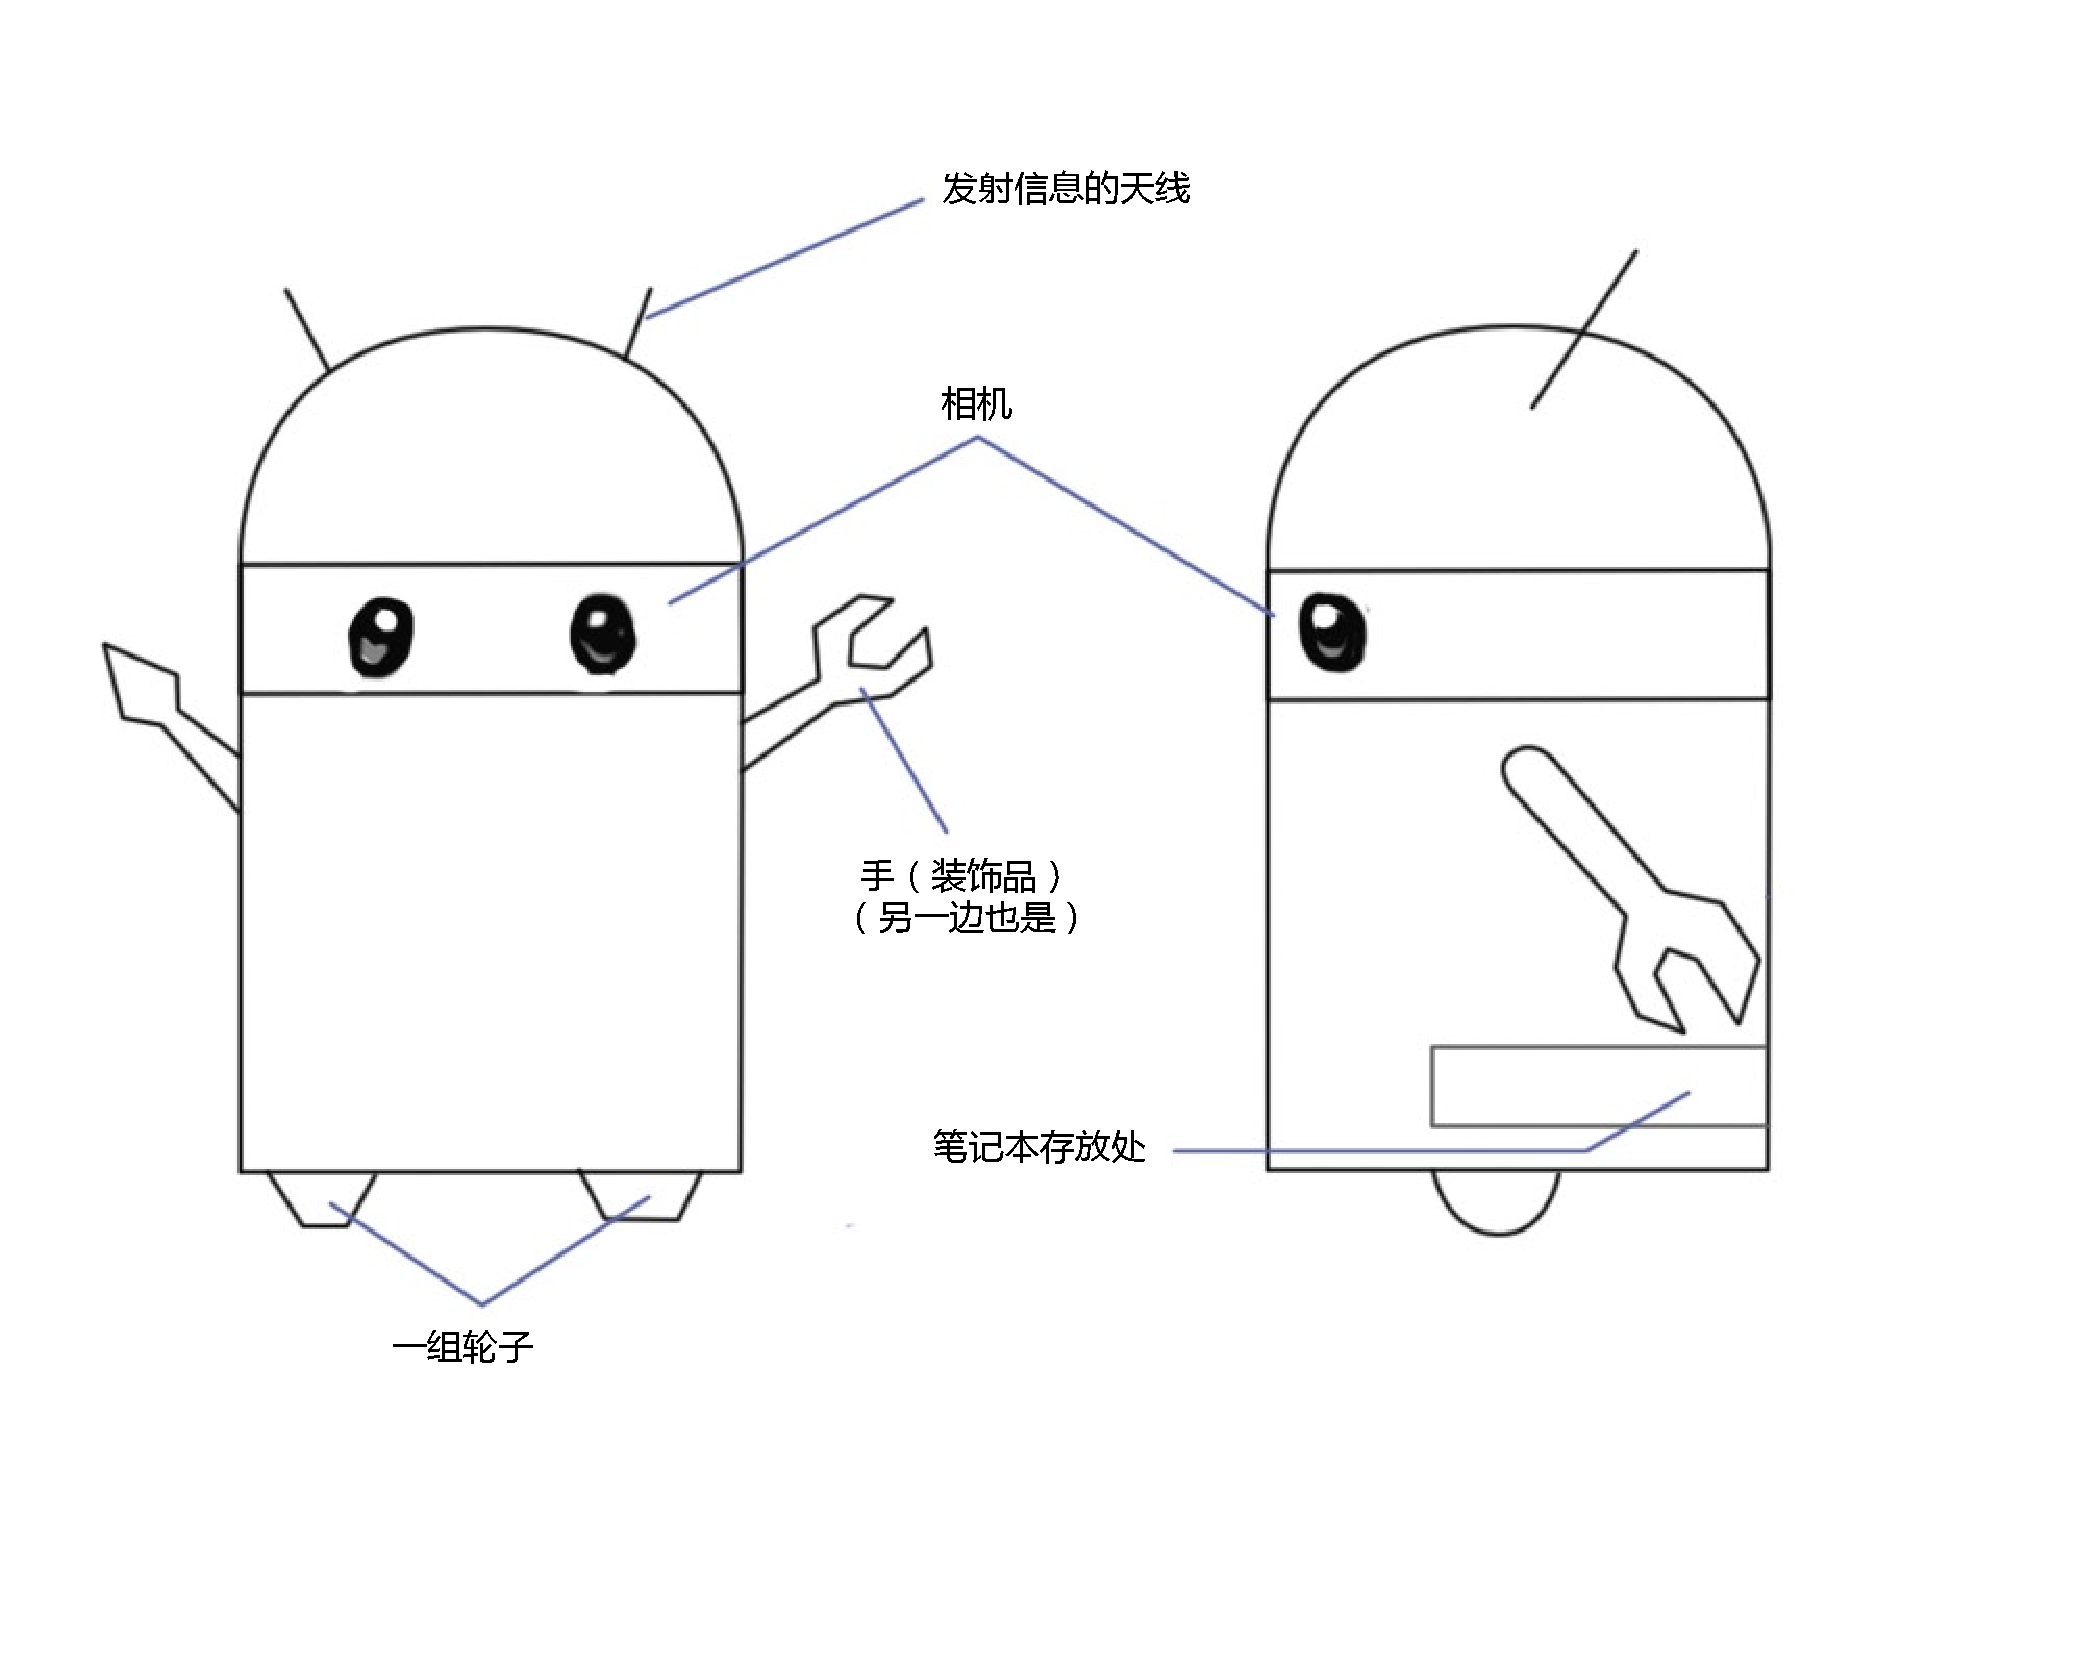
\includegraphics[width=0.7\textwidth]{whatIsSLAM/carrot.pdf}
	\caption{小萝卜设计图。左边:正视图;右边:侧视图。设备有相机、轮子、笔记本,手是装饰品。}
	\label{fig:carrot}
\end{figure}

先不要管它这个简笔画的风格。另外,虽然有点像“安卓”,但它并不是靠安卓系统来计算的。我们把一台笔记本塞进了它的后备箱内(方便我们随时拿出来调试程序)。它能做点什么呢?

我们希望小萝卜具有\textbf{自主运动能力},这是非常基本的功能。虽然世界上也有放在桌面像摆件一样的机器人,能够和人说话或播放音乐(听说还卖得不错),不过一台平板电脑完全可以胜任这些事情。作为机器人,我们希望小萝卜能够在房间里自由移动。不管我们在哪里招呼一声,它都会滴溜溜地走过来。

你会发现自主运动能力是许多高级功能的前提。不管是扫地也好搬东西也好,首先要让它动起来。要移动就得有轮子和电机,所以我们在小萝卜的下方安装了轮子(足式机器人步态很复杂,留给自动化所的博士们发论文去吧)。有了轮子,机器人就能够四处行动了,但不加规划和控制的话,小萝卜不知道行动的目标,就只能四处乱走,更糟糕的情况下会撞上墙造成损毁。而要规划和控制,首先需要\textbf{感知}周边的环境。为此,我们在它的脑袋上安装了一个相机。安装相机的主要动机,是考虑到这样一个机器人\textbf{和人类非常相似}——从画面上一眼就能看出。有眼睛、大脑和四肢的人类,能够在任意环境里轻松自在地行走、探索,我们(天真地)觉得机器人也能够完成这件事。为了使小萝卜能够探索一个房间,它至少需要知道两件事:

\begin{enumerate}
	\item 我在什么地方?——定位。
	\item 周围环境是什么样?——建图。
\end{enumerate}

“定位”和“建图”,可以看成感知的“内外之分”。作为一个“内外兼修”的小萝卜,一方面要明白自身的\textbf{状态}(即位置),另一方面也要了解外在的\textbf{环境}(即地图)。当然,解决这两个问题的方法非常多。比方说,我们可以在房间地板上铺设导引线,在墙壁上贴识别二维码,在桌子上放置无线电定位设备(这其实是现在很多仓储物流机器人的做法)。如果在室外,还可以在小萝卜脑袋上安装GPS信号接收器(像手机或汽车一样)。有了这些东西之后,定位问题是否已经解决了呢?我们不妨把这些传感器(见\autoref{fig:sensors})分为两类。

一类传感器是\textbf{携带于机器人本体上}的,例如机器人的轮式编码器、相机、激光传感器,等等。另一类是\textbf{安装于环境中}的,例如前面讲的导轨、二维码标志,等等。安装于环境中的传感设备,通常能够直接测量到机器人的位置信息,简单有效地解决定位问题。然而,由于它们要求环境必须可以人工布置,在一定程度上限制了机器人的使用范围。比方说,室内环境往往没有GPS信号,绝大多数园区无法铺设导轨,这时该怎么做定位呢?

\begin{figure}[!ht]
	\centering
	\includegraphics[width=1.0\textwidth]{whatIsSLAM/sensors.pdf}
	\caption{一些传感器。(a)利用二维码进行定位的增强现实软件;(b)GPS定位装置;(c)铺设导轨的小车;(d)激光雷达;(e)IMU单元;(f)双目相机。}
	\label{fig:sensors}
\end{figure}

我们看到,这类传感器\textbf{约束}了外部环境。只有在这些约束满足时,基于它们的定位方案才能工作。反之,当约束无法满足时,我们就没法进行定位了。所以说,虽然这类传感器简单可靠,但它们无法提供一个普遍的、通用的解决方案。相对地,那些携带于机器人本体上的传感器,比如激光传感器、相机、轮式编码器、惯性测量单元(Inertial Measurement Unit,IMU)等,它们测到的通常都是一些间接的物理量而不是直接的位置数据。例如,轮式编码器会测到轮子转动的角度,IMU测量运动的角速度和加速度,相机和激光传感器则读取外部环境的某种观测数据。我们只能通过一些间接的手段,从这些数据推算自己的位置。虽然这听上去是一种迂回战术,但更明显的好处是,它没有对环境提出任何要求\footnote{话虽如此,实际我们至少要求传感器在该环境下能够工作,所以不要举一些“轮式编码器在宇宙空间中没法工作,相机在黑屋子里看不见东西”的极端例子。},从而使得这种定位方案可适用于未知环境。

%\clearpage
回顾前面讨论过的SLAM定义,我们在SLAM中非常强调未知环境。所以在理论上,我们不限制小萝卜的使用环境\footnote{不过现实中我们都会有一个大概的范围,例如室内和室外的区分。},这意味着我们没法假设像GPS或导轨这样的外部传感器都能顺利工作。因此,使用携带式的传感器来完成SLAM是我们重点关心的问题。特别地,当谈论视觉SLAM时,我们主要是指如何用\textbf{相机}解决定位和建图问题。同样,如果传感器主要是激光,那就称为激光SLAM。激光SLAM相对成熟,比如2005年的《概率机器人》\textsuperscript{\cite{Thrun2005}}就介绍了许多激光SLAM的知识,在ROS里你也能找到许多关于激光定位、激光建图的现成软件。

视觉SLAM是本书的主题,所以我们尤其关心小萝卜的眼睛能够做些什么事。SLAM中使用的相机与我们平时见到的单反摄像头并不是同一个东西。它更加简单,通常不携带昂贵的镜头,而是以一定速率拍摄周围的环境,形成一个连续的视频流。普通的摄像头能以每秒钟30张图片的速度采集图像,高速相机则更快一些。按照工作方式的不同,相机可以分为单目相机(Monocular)、双目相机(Stereo)和深度相机(RGB-D)三大类,如\autoref{fig:camera}所示。直观看来,单目相机只有一个摄像头,双目有两个,而RGB-D原理较复杂,除了能够采集到彩色图片之外,还能读出每个像素与相机之间的距离。深度相机通常携带多个摄像头,工作原理和普通相机不尽相同,在第5讲会详细介绍其工作原理,此处读者只需有一个直观概念即可。此外,SLAM中还有全景相机\textsuperscript{\cite{Pretto2011}}、Event相机\textsuperscript{\cite{Rueckauer2016}}等特殊或新兴的种类。虽然偶尔能看到它们在SLAM中的应用,不过到目前为止还没有成为主流。从样子上看,小萝卜使用的似乎是水平的双目相机。

\begin{figure}[!ht]
	\centering
	\includegraphics[width=0.8\textwidth]{whatIsSLAM/camera.pdf}
	\caption{形形色色的相机:单目、双目和深度相机。}
	\label{fig:camera}
\end{figure}

我们来分别看一看各种相机用来做SLAM时有什么特点。

\subsubsection{单目相机}
只使用一个摄像头进行SLAM的做法称为单目SLAM(Monocular SLAM)。这种传感器结构特别简单,成本特别低,所以单目SLAM非常受研究者关注。你肯定见过单目相机的数据:照片。是的,作为一张照片,它有什么特点呢?

照片本质上是拍摄某个场景(Scene)在相机的成像平面上留下的一个\textbf{投影}。\textbf{它以二维的形式记录了三维的世界。}显然,这个过程丢掉了场景的一个维度,也就是所谓的深度(或距离)。在单目相机中,我们无法通过单张图片来计算场景中物体与相机之间的\textbf{距离}(远近)。之后我们会看到,这个距离将是SLAM中非常关键的信息。由于我们人类见过大量的图像,形成了一种天生的直觉,对大部分场景都有一个直观的\textbf{距离感(空间感)},它可以帮助我们判断图像中物体的远近关系。比如说,我们能够辨认出图像中的物体,并且知道其大致的大小;比如,近处的物体会挡住远处的物体,而太阳、月亮等天体一般在很远的地方;再如,物体受光照后会留下影子,等等。这些信息都可以帮助我们判断物体的远近,但也存在一些情况会使这种距离感失效,这时我们就无法判断物体的远近及其真实大小了。\autoref{fig:why-depth}~就是这样一个例子。在这张图像中,我们无法仅通过它来判断后面那些小人是真实的人,还是小型模型。除非我们转换视角,观察场景的三维结构。换言之,在单张图像里,你无法确定一个物体的真实大小。它可能是一个\textbf{很大但很远}的物体,也可能是一个\textbf{很近但很小}的物体。由于近大远小的透视关系,它们可能在图像中变成同样大小的样子。

\begin{figure}[!htp]
	\centering
	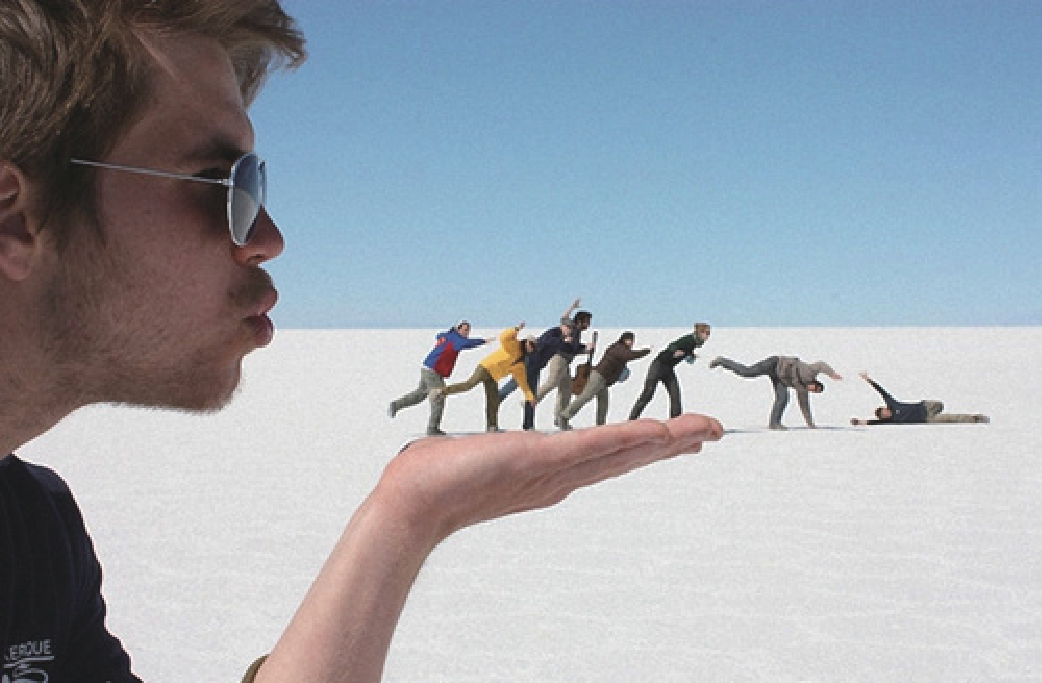
\includegraphics[width=0.7\textwidth]{whatIsSLAM/why-depth.pdf}
	\caption{单目视觉中的尴尬:不知道深度时,手掌上的人是真人还是模型?}
	\label{fig:why-depth}
\end{figure}

由于单目相机拍摄的图像只是三维空间的二维投影,所以,如果真想恢复三维结构,必须改变相机的视角。在单目SLAM中也是同样的原理。我们必须移动相机,才能估计它的\textbf{运动}(Motion),同时估计场景中物体的远近和大小,不妨称之为\textbf{结构}(Structure)。那么,怎么估计这些运动和结构呢?想象你坐在一辆运动的列车中。如果列车往右移动,那么我们看到的东西就会往左边移动——这就给我们推测运动带来了信息。另一方面,我们还知道:\textbf{近处的物体移动快,远处的物体则运动缓慢,极远处(无穷远处)的物体(如太阳、月亮)看上去是不动的}。于是,当相机移动时,这些物体在图像上的运动就形成了\textbf{视差}(disparity)。通过视差,我们就能定量地判断哪些物体离得远,哪些物体离得近。

然而,即使我们知道了物体远近,它们仍然只是一个相对的值。比如我们在看电影时,虽然能够知道电影场景中哪些物体比另一些大,但无法确定电影里那些物体的“真实尺度”:那些大楼是真实的高楼大厦,还是放在桌上的模型?而摧毁大厦的是真实怪兽,还是穿着特摄服装的演员?直观地说,如果把相机的运动和场景大小同时放大两倍,单目相机所看到的像是一样的。同样地,把这个大小乘以任意倍数,我们都将看到一样的景象。这说明,单目SLAM估计的轨迹和地图将与真实的轨迹和地图相差一个因子,也就是所谓的\textbf{尺度}(Scale)\footnote{数学上的原因将会在视觉里程计一讲中解释。}。由于单目SLAM无法仅凭图像确定这个真实尺度,所以又称为\textbf{尺度不确定性}(Scale Ambiguity)。

平移之后才能计算深度,以及无法确定真实尺度,这两件事情给单目SLAM的应用造成了很大的麻烦。其根本原因是通过单张图像无法确定深度。所以,为了得到这个深度,人们开始使用双目和深度相机。

\subsubsection{双目相机和深度相机}

使用双目相机和深度相机的目的,在于通过某种手段测量物体与我们之间的距离,克服单目相机无法知道距离的缺点。一旦知道了距离,场景的三维结构就可以通过单个图像恢复出来,同时消除尺度不确定性。尽管都是为了测量距离,但双目相机与深度相机测量深度的原理是不一样的。双目相机由两个单目相机组成,但这两个相机之间的距离﹝称为\textbf{基线}(Baseline)﹞是已知的。我们通过这个基线来估计每个像素的空间位置——这和人眼非常相似。我们人类可以通过左右眼图像的差异判断物体的远近,在计算机上也是同样的道理(见\autoref{fig:stereo})。如果对双目相机进行拓展,也可以搭建多目相机,不过本质上并没有什么不同。

\begin{figure}[!ht]
	\centering
	\includegraphics[width=1.0\textwidth]{whatIsSLAM/stereo.pdf}
	\caption{双目相机的数据:左眼图像,右眼图像。通过左右眼的差异,能够判断场景中物体与相机之间的距离。}
	\label{fig:stereo}
\end{figure}

计算机上的双目相机需要大量的计算才能(不太可靠地)估计每一个像素点的深度,相比于人类真是非常笨拙\footnote{我三个月大的女儿已经能够辨认并抓取放在她面前的玩具了,我觉得她比许多大学实验室里的机器人都要智能。}。双目相机测量到的深度范围与基线相关。基线距离越大,能够测量到的就越远,所以无人车上搭载的双目通常会是个很大的家伙。双目相机的距离估计是比较左右眼的图像获得的,并不依赖其他传感设备,所以它既可以应用在室内,亦可应用于室外。双目或多目相机的缺点是配置与标定均较为复杂,其深度量程和精度受双目的基线与分辨率所限,而且视差的计算非常消耗计算资源,需要使用GPU和FPGA设备加速后,才能实时输出整张图像的距离信息。因此在现有的条件下,计算量是双目的主要问题之一。

深度相机(又称RGB-D相机,在本书中主要使用RGB-D这个名称)是2010年左右开始兴起的一种相机,它最大的特点是可以通过红外结构光或Time-of-Flight(ToF)原理,像激光传感器那样,通过主动向物体发射光并接收返回的光,测出物体与相机之间的距离。这部分并不像双目相机那样通过软件计算来解决,而是通过物理的测量手段,所以相比于双目相机可节省大量的计算(见\autoref{fig:rgbd})。目前常用的RGB-D相机包括Kinect/Kinect V2、Xtion Pro Live、RealSense等,在一些手机上人们也用它来识别人脸。不过,现在多数RGB-D相机还存在测量范围窄、噪声大、视野小、易受日光干扰、无法测量透射材质等诸多问题,在SLAM方面,主要用于室内,室外则较难应用。

\begin{figure}[!ht]
	\centering
	\includegraphics[width=0.8\textwidth]{whatIsSLAM/rgbd.pdf}
	\caption{RGB-D数据:深度相机可以直接测量物体的图像和距离,从而恢复三维结构。}
	\label{fig:rgbd}
\end{figure}

我们讨论了几种常见的相机,相信通过以上的说明,你已经对它们有了直观的了解。现在,想象相机在场景中运动的过程,我们将得到一系列连续变化的图像\footnote{你可以用手机录个小视频试试。}。视觉SLAM的目标,是通过这样的一些图像,进行定位和地图构建。这件事情并没有想象的那么简单。它不是某种算法,只要我们输入数据,就可以往外不断地输出定位和地图信息了。SLAM需要一个完善的算法框架,而经过研究者们长期的努力工作,现有这个框架已经定型了。

\section{经典视觉SLAM框架}
下面来看经典的视觉SLAM框架(\autoref{fig:overflow}),了解一下视觉SLAM究竟由哪几个模块组成。

\begin{figure}[!htp]
	\centering
	\includegraphics[width=0.8\textwidth]{whatIsSLAM/overflow.pdf}
	\caption{整体视觉SLAM流程图。}
	\label{fig:overflow}
\end{figure}

整个视觉SLAM流程包括以下步骤。
\begin{enumerate}
	\item 传感器信息读取。在视觉SLAM中主要为相机图像信息的读取和预处理。如果是在机器人中,还可能有码盘、惯性传感器等信息的读取和同步。
	\item \textbf{视觉里程计}(Visual Odometry,VO)。视觉里程计的任务是估算相邻图像间相机的运动,以及局部地图的样子。VO又称为前端(Front End)。
	\item \textbf{后端优化}(Optimization)。后端接受不同时刻视觉里程计测量的相机位姿,以及回环检测的信息,对它们进行优化,得到全局一致的轨迹和地图。由于接在VO之后,又称为后端(Back End)。
	\item \textbf{回环检测}(Loop Closing)。回环检测判断机器人是否到达过先前的位置。如果检测到回环,它会把信息提供给后端进行处理。
	\item \textbf{建图}(Mapping)。它根据估计的轨迹,建立与任务要求对应的地图。
\end{enumerate}

经典的视觉SLAM框架是过去十几年的研究成果。这个框架本身及其所包含的算法已经基本定型,并且已经在许多视觉程序库和机器人程序库中提供。依靠这些算法,我们能够构建一个视觉SLAM系统,使之在正常的工作环境里实时定位与建图。因此,我们说,\textbf{如果把工作环境限定在静态、刚体,光照变化不明显、没有人为干扰的场景},那么,这种场景下的SLAM技术已经相当成熟\textsuperscript{\cite{Cadena2016}}。

读者可能还没有理解上面几个模块的概念,下面就来详细介绍各个模块具体的任务。但是,准确理解其工作原理需要一些数学知识,我们将放到本书的第二部分进行。这里读者只需对各模块有一个直观的、定性的理解即可。

\subsection{视觉里程计}
视觉里程计关心\textbf{相邻图像}之间的相机运动,最简单的情况当然是两张图像之间的运动关系。例如,当看到\autoref{fig:cameramotion}时,我们会自然地反应出右图应该是左图向左旋转一定角度的结果(在视频情况下感觉会更加自然)。我们不妨思考一下:自己是怎么知道“向左旋转”这件事情的呢?人类早已习惯于用眼睛探索世界,估计自己的位置,但又往往难以用理性的语言描述我们的直觉\footnote{在很多涉及计算机视觉和机器学习的任务中,情况都是这样。拜近几年深度学习所赐,我们连机器是怎么计算的都已经看不懂了。}。看到\autoref{fig:cameramotion}时,我们会自然地认为,这个场景中离我们近的是吧台,远处是墙壁和黑板。当相机向左转动时,吧台离我们近的部分出现在视野中,而右侧远处的柜子则移出了视野。通过这些信息,我们判断相机应该是向左旋转了。

\begin{figure}[!ht]
	\centering
	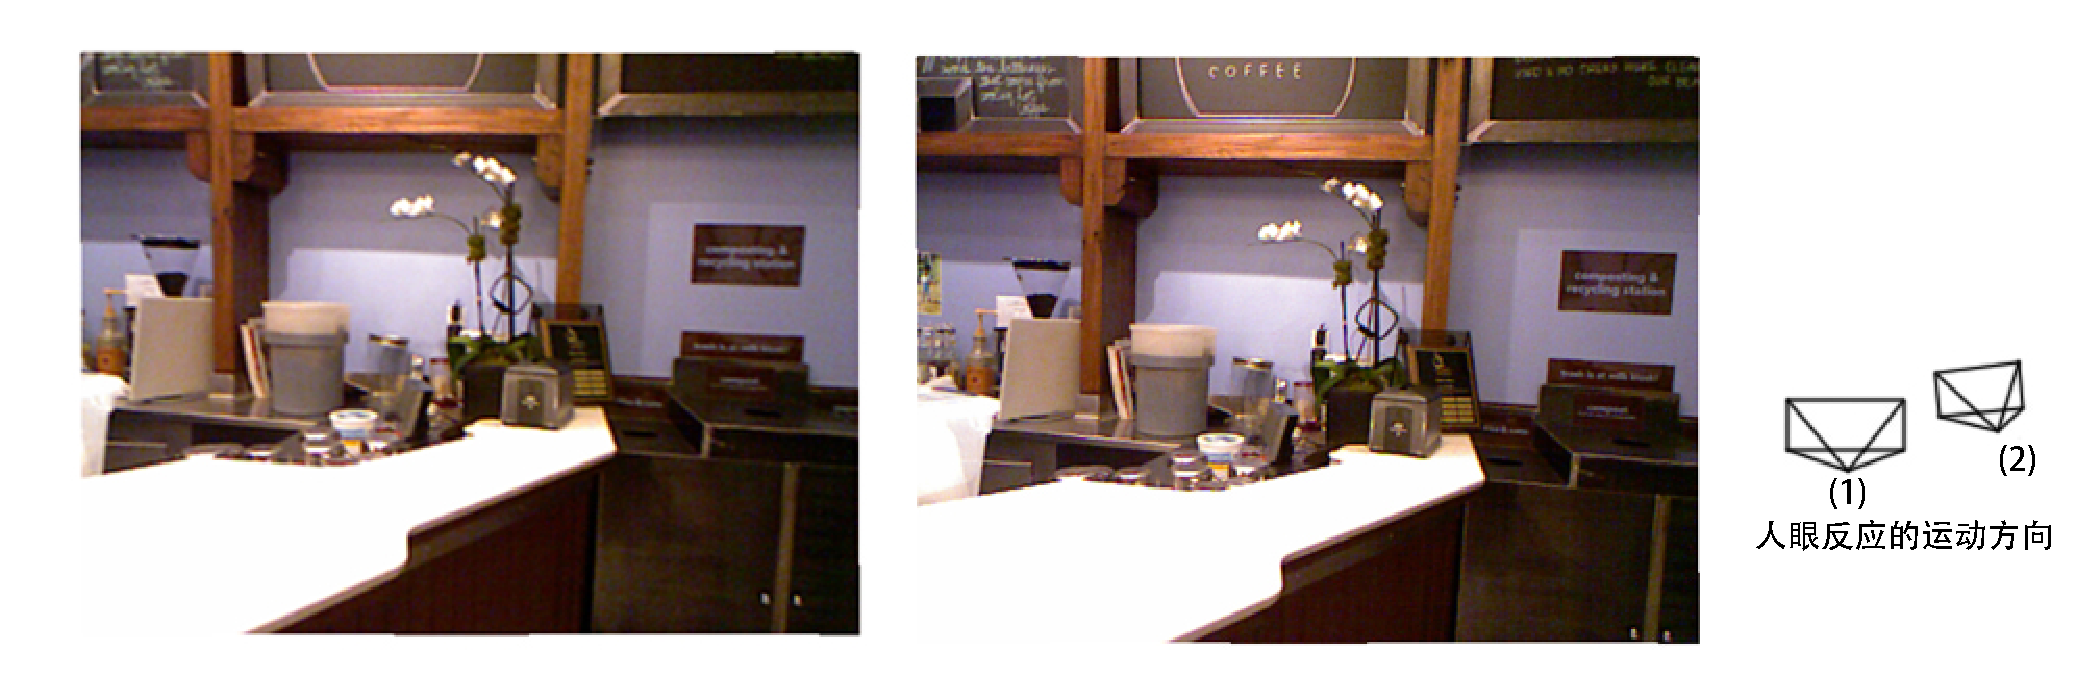
\includegraphics[width=0.8\textwidth]{whatIsSLAM/cameramotion.pdf}
	\caption{相机拍摄到的图片与人眼反应的运动方向。}
	\label{fig:cameramotion}
\end{figure}

但是,如果进一步问:能否确定旋转了多少度,平移了多少厘米?我们就很难给出一个确切的答案了。因为我们的直觉对这些具体的数字并不敏感。但是,在计算机中,又必须精确地测量这段运动信息。所以我们要问:\textbf{计算机是如何通过图像确定相机的运动的呢?}

前面也提过,在计算机视觉领域,人类在直觉上看来十分自然的事情,在计算机视觉中却非常困难。图像在计算机里只是一个数值矩阵。这个矩阵里表达着什么东西,计算机毫无概念(这也正是现在机器学习要解决的问题)。而在视觉SLAM中,我们只能看到一个个像素,知道它们是某些空间点在相机的成像平面上投影的结果。所以,为了定量地估计相机运动,必须先\textbf{了解相机与空间点的几何关系}。

要讲清这个几何关系以及VO的实现方法,需要铺垫一些背景知识。在这里我们先让读者对VO有个直观的概念。现在只需知道,VO能够通过相邻帧间的图像估计相机运动,并恢复场景的空间结构。称它为“里程计”是因为它和实际的里程计一样,只计算相邻时刻的运动,而和再往前的过去的信息没有关联。在这一点上,VO就像一种只有短时间记忆的物种(不过可以不限于两帧,数量可以更多一些,例如5-10帧)。

现在,假定我们已有了一个视觉里程计,估计了两张图像间的相机运动。那么,只要把相邻时刻的运动“串”起来,就构成了机器人的运动轨迹,从而解决了定位问题。另一方面,我们根据每个时刻的相机位置,计算出各像素对应的空间点的位置,就得到了地图。这么说来,有了VO,是不是就解决了SLAM问题呢?

视觉里程计确实是SLAM的关键,我们也会花大量的篇幅来介绍它。然而,仅通过视觉里程计来估计轨迹,将不可避免地出现\textbf{累积漂移}(Accumulating Drift)。这是由于视觉里程计(在最简单的情况下)只估计两个图像间的运动造成的。我们知道,每次估计都带有一定的误差,而由于里程计的工作方式,先前时刻的误差将会传递到下一时刻,导致经过一段时间之后,估计的轨迹将不再准确(见\autoref{fig:loopclosure})。比方说,机器人先向左转$90^\circ$,再向右转$90^\circ$。由于误差,我们把第一个$90^\circ$估计成了$89^\circ$。那我们就会尴尬地发现,向右转之后机器人的估计位置并没有回到原点。更糟糕的是,即使之后的估计完全准确,与真实值相比,都会带上这$-1^\circ$的误差。

\begin{figure}[!htp]
	\centering
	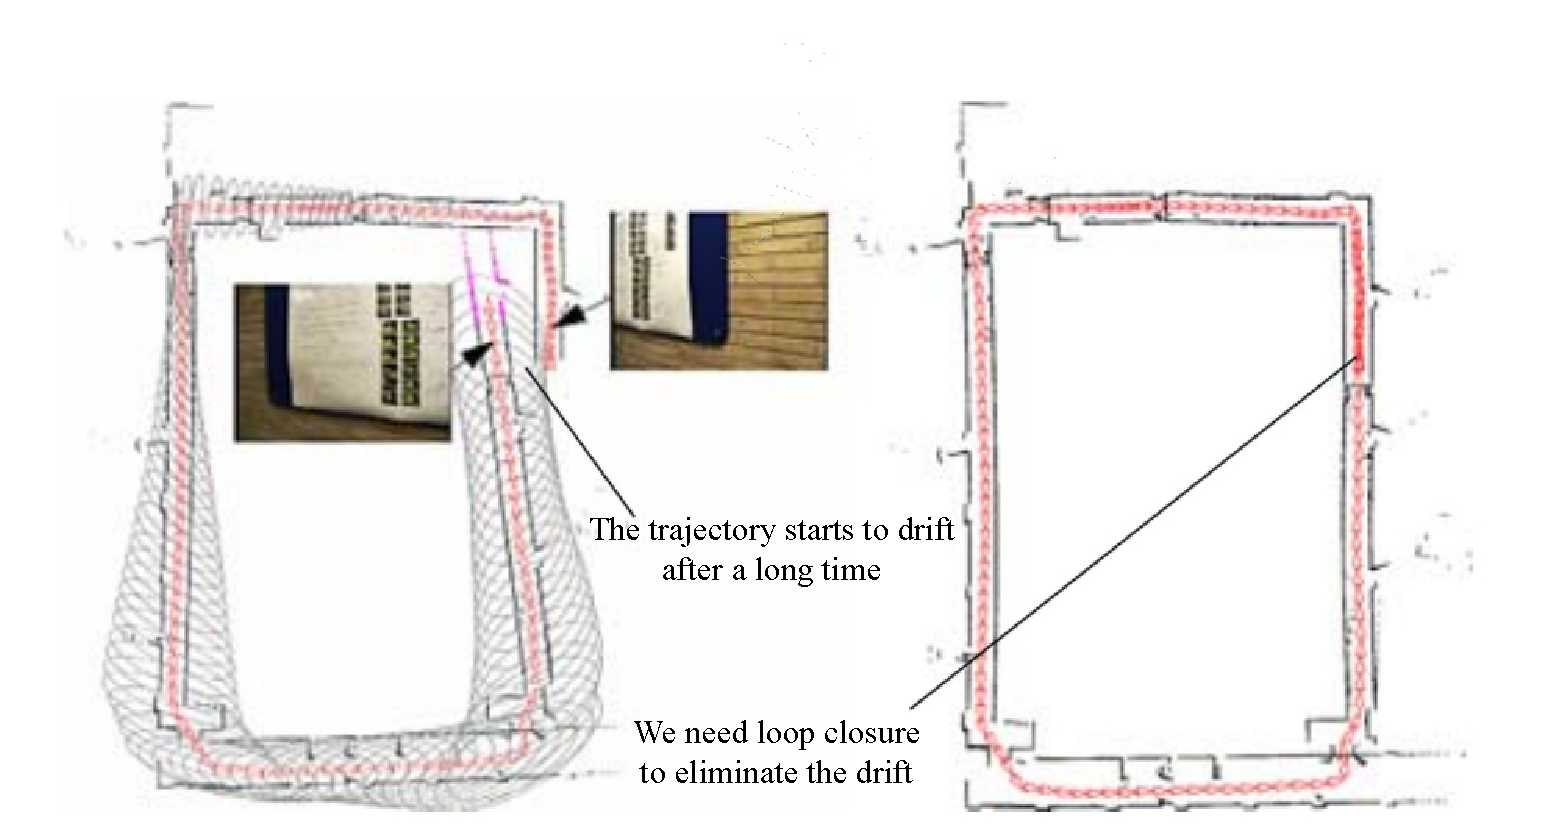
\includegraphics[width=0.8\textwidth]{whatIsSLAM/loopclosure.pdf}
	\caption{累积误差与回环检测的校正结果\textsuperscript{\cite{Newman2005}}。}
	\label{fig:loopclosure}
\end{figure}

这也就是所谓的\textbf{漂移}(Drift)。它将导致我们无法建立一致的地图。你会发现原本直的走廊变成了斜的,而原本$90^\circ$的直角变成了歪的——这实在是一件令人难以忍受的事情!为了解决漂移问题,我们还需要两种技术:\textbf{后端优化}\footnote{更多时候称为后端(Back End)。由于主要使用的是优化方法,故称为后端优化。}和\textbf{回环检测}。回环检测负责把“机器人回到原始位置”的事情检测出来,而后端优化则根据该信息,校正整个轨迹的形状。

\subsection{后端优化}
笼统地说,后端优化主要指处理SLAM过程中\textbf{噪声}的问题。虽然我们很希望所有的数据都是准确的,然而现实中,再精确的传感器也带有一定的噪声。便宜的传感器测量误差较大,昂贵的可能会小一些,有的传感器还会受磁场、温度的影响。所以,除了解决“如何从图像估计出相机运动”之外,我们还要关心这个估计带有多大的噪声,这些噪声是如何从上一时刻传递到下一时刻的,而我们又对当前的估计有多大的自信。后端优化要考虑的问题,就是如何从这些带有噪声的数据中估计整个系统的状态,以及这个状态估计的不确定性有多大——这称为最大后验概率估计(Maximum-a-Posteriori,MAP)。这里的状态既包括机器人自身的轨迹,也包含地图。

相对地,视觉里程计部分有时被称为“前端”。在SLAM框架中,前端给后端提供待优化的数据,以及这些数据的初始值。而后端负责整体的优化过程,它往往面对的只有数据,不必关心这些数据到底来自什么传感器。\textbf{在视觉SLAM中,前端和计算机视觉研究领域更为相关,比如图像的特征提取与匹配等,后端则主要是滤波与非线性优化算法。}

从历史意义上来说,现在我们称为后端优化的部分,很长一段时间直接被称为“SLAM研究”。早期的SLAM问题是一个\textbf{状态估计}问题——正是后端优化要解决的东西。在最早提出SLAM的一系列论文中,当时的人们称它为“空间状态不确定性的估计”(Spatial Uncertainty)\textsuperscript{\cite{Smith1986, Smith1990}}。虽然有一些晦涩,但也确实反映出了SLAM问题的本质:\textbf{对运动主体自身和周围环境空间不确定性的估计}。为了解决SLAM问题,我们需要状态估计理论,把定位和建图的不确定性表达出来,然后采用滤波器或非线性优化,估计状态的均值和不确定性(方差)。状态估计与非线性优化的具体内容将在第6讲、第9讲和第10讲介绍。让我们暂时跳过它的原理说明,继续往下介绍。

\subsection{回环检测}

回环检测,又称闭环检测(Loop Closure Detection/Loop Closingn),主要解决位置估计\textbf{随时间漂移}的问题。怎么解决呢?假设实际情况下机器人经过一段时间的运动后回到了原点,但是由于漂移,它的位置估计值却没有回到原点。怎么办呢?我们想,如果有某种手段,让机器人知道“回到了原点”这件事,或者把“原点”识别出来,我们再把位置估计值“拉”过去,就可以消除漂移了。这就是所谓的回环检测。

回环检测与“定位”和“建图”二者都有密切的关系。事实上,我们认为,地图存在的主要意义是让机器人知晓自己到过的地方。为了实现回环检测,我们需要让机器人具有\textbf{识别到过的场景}的能力。它的实现手段有很多。例如像前面说的那样,我们可以在机器人下方设置一个标志物(如一张二维码图片)。它只要看到了这个标志,就知道自己回到了原点。但是,该标志物实质上是一种环境中的传感器,对应用环境做了限制(万一不能贴二维码怎么办?)。我们更希望机器人能使用携带的传感器——也就是图像本身,来完成这一任务。例如,可以判断\textbf{图像间的相似性}来完成回环检测。这一点和人是相似的。当我们看到两张相似的图片时,容易辨认它们来自同一个地方。如果回环检测成功,可以显著地减小累积误差。所以,视觉回环检测实质上是一种计算图像数据相似性的算法。由于图像的信息非常丰富,使得正确检测回环的难度降低了不少。

在检测到回环之后,我们会把“A与B是同一个点”这样的信息告诉后端优化算法。然后,后端根据这些新的信息,把轨迹和地图调整到符合回环检测结果的样子。这样,如果我们有充分而且正确的回环检测,就可以消除累积误差,得到全局一致的轨迹和地图。

%对于视觉SLAM,多数系统采用目前较为成熟的词袋模型(Bag-of-Words, BoW)。词袋模型把图像中的视觉特征(SIFT, SURF等)聚类,然后建立词典,进而寻找每个图中含有哪些“单词”(word)。也有研究者使用传统模式识别的方法,把回环检测建构成一个分类问题,训练分类器进行分类。
%
%但是回环检测的困难也是存在的,主要在于\textbf{错误的检测结果可能使地图变得很糟糕}。错误可分为两类:1.假阳性(False Positive),又称感知偏差(Perceptual Aliasing),指事实上不同的场景被当成了同一个。这主要来自一些看似相同的场景,然而实际上是两个不同的地方。这种情况在人工建筑物普遍存在,例如一幢楼里很多门、窗、厕所、走廓,都十分地相似,很容易被当成同一个。2. 假阴性(False Negative),又称感知变异(Perceptual Variability),指实际上同一个场景被当成了两个。在视觉SLAM中,这种情况主要发生在光照变化的场合。例如清晨的阳光洒进窗户,朦胧一片,而正午时分,光线清晰,景物错落可见。虽然人能否通过直觉辨别,但它在计算机图像中的差异如此之大,很难认出这是同一个窗户。
%
%一个好的视觉回环检测算法应该尽量避免出现这两种错误。因此,它要保证两点:
%
%\begin{enumerate}
%	\item 检测出的回环应该是对的。
%	\item 实际发生回环的时候,应该被检测出来。
%\end{enumerate}
%
%前者称为准确率(Perception),后者称为召回率(Recall)。尽管不是必然,但对同一个算法来说,这两者往往是矛盾的:准确率的提升意味着更严格的检测,使得差的回环无法提取出来——从而可能忽略掉真实存在的回环。研究者们常常用准确率-召回率曲线来评价一个回环检测算法的好坏。我们自然希望能够有准确率和召回率都很高的回环检测算法,但现实往往不尽如人意。

% 如果我们有了良好的回环检测和后端优化算法,就能得到一个全局一致性较好的轨迹了。剩下的工作,就是建立一个良好的地图。

\subsection{建图}
建图(Mapping)是指构建地图的过程。地图(见\autoref{fig:map})是对环境的描述,但这个描述并不是固定的,需要视SLAM的应用而定。

\begin{figure}[!htp]
	\centering
	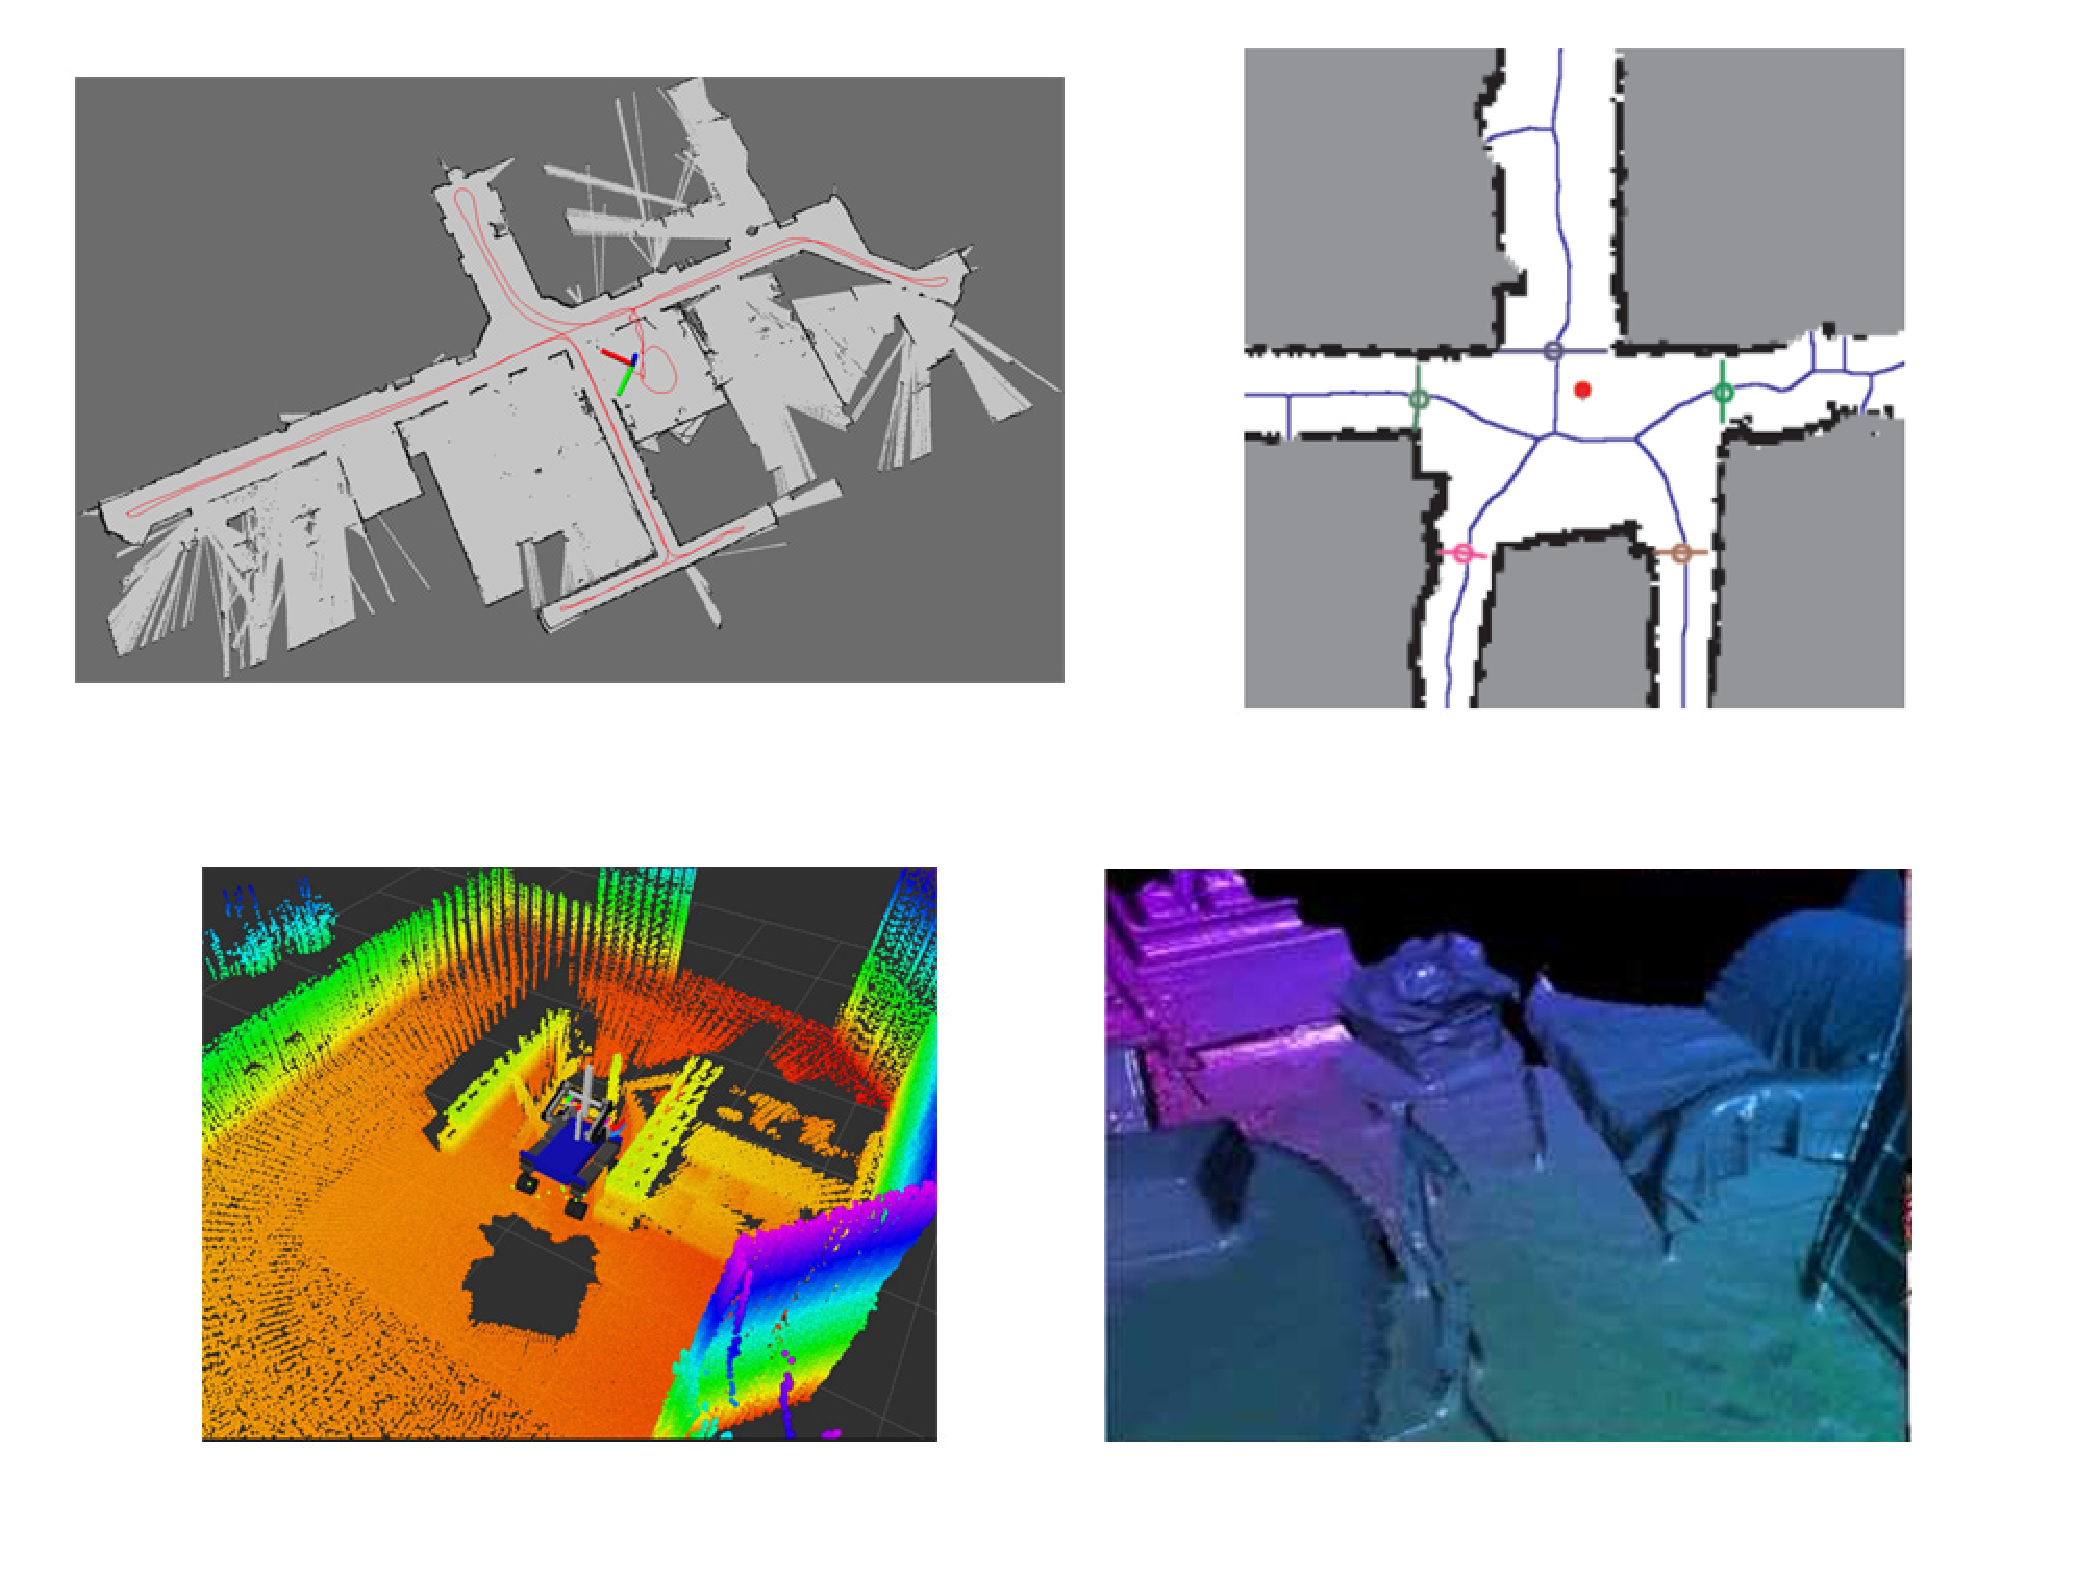
\includegraphics[width=0.8\textwidth]{whatIsSLAM/map.pdf}
	\caption{形形色色的地图\textsuperscript{\cite{Beeson2010}}。}
	\label{fig:map}
\end{figure}

对于家用扫地机器人来说,这种主要在低矮平面里运动的机器人,只需要一个二维的地图,标记哪里可以通过,哪里存在障碍物,就够它在一定范围内导航了。而对于一个相机,它有6自由度的运动,我们至少需要一张三维的地图。有些时候,我们想要一个漂亮的重建结果,不仅是一组空间点,还需要带纹理的三角面片。另一些时候,我们又不关心地图的样子,只需要知道“A点到B点可通过,而B点到C点不行”这样的事情。甚至,有时不需要地图,或者地图可以由其他人提供,例如,行驶的车辆往往可以得到已绘制好的当地地图。

对于地图,我们有太多的想法和需求。因此,相比于前面提到的视觉里程计、回环检测和后端优化,建图并没有一个固定的形式和算法。一组空间点的集合也可以称为地图,一个漂亮的3D模型亦是地图,一个标记着城市、村庄、铁路、河道的图片还是地图。地图的形式随SLAM的应用场合而定。大体上讲,可以分为\textbf{度量地图}与\textbf{拓扑地图}两种。

\clearpage

\subsubsection{度量地图(Metric Map)}
度量地图强调精确地表示地图中物体的位置关系,通常用稀疏(Sparse)与稠密(Dense)对其分类。稀疏地图进行了一定程度的抽象,并不需要表达所有的物体。例如,我们选择一部分具有代表意义的东西,称之为路标(Landmark),那么一张稀疏地图就是由路标组成的地图,而不是路标的部分就可以忽略掉。相对地,稠密地图着重于建模所有看到的东西。对于定位来说,稀疏路标地图就足够了。而用于导航时,则往往需要稠密的地图(否则撞上两个路标之间的墙怎么办?)。稠密地图通常按照某种分辨率,由许多个小块组成。对于二维度量地图是许多个小格子(Grid),而对于三维度量地图则是许多小方块(Voxel)。一般地,一个小块含有占据、空闲、未知三种状态,以表达该格内是否有物体。当查询某个空间位置时,地图能够给出该位置是否可以通过的信息。这样的地图可以用于各种导航算法,如A*、D*\footnote{\url{https://en.wikipedia.org/wiki/A*_search_algorithm}}等,为机器人研究者所重视。但是我们也看到,这种地图需要存储每一个格点的状态,会耗费大量的存储空间,而且多数情况下地图的许多细节部分是无用的。另一方面,大规模度量地图有时会出现一致性问题。很小的一点转向误差,可能会导致两间屋子的墙出现重叠,使地图失效。

\subsubsection{拓扑地图(Topological Map)}
相比于度量地图的精确性,拓扑地图则更强调地图元素之间的关系。拓扑地图是一个图(Graph),由节点和边组成,只考虑节点间的连通性,例如A、B点是连通的,而不考虑如何从A点到达B点。它放松了地图对精确位置的需要,去掉了地图的细节问题,是一种更为紧凑的表达方式。然而,拓扑地图不擅长表达具有复杂结构的地图。如何对地图进行分割形成结点与边,又如何使用拓扑地图进行导航与路径规划,仍是有待研究的问题。

\section{SLAM问题的数学表述}

通过前面的介绍,读者应该对SLAM中各个模块的组成和主要功能有了直观的了解。但仅仅靠直观印象并不能帮助我们写出可以运行的程序。我们要把它上升到理性层次,也就是用数学语言来描述SLAM过程。我们会用到一些变量和公式,但请读者放心,我会尽量让它保持足够地清楚。

假设小萝卜正携带着某种传感器在未知环境里运动,怎么用数学语言描述这件事呢?首先,由于相机通常是在某些时刻采集数据的,所以我们也只关心这些时刻的位置和地图。这就把一段连续时间的运动变成了离散时刻$t=1, \cdots, K$当中发生的事情。在这些时刻,用$\bm{x}$表示小萝卜自身的位置。于是各时刻的位置就记为$ \bm{x}_1, \cdots, \bm{x}_K$,它们构成了小萝卜的轨迹。地图方面,我们假设地图是由许多个\textbf{路标}(Landmark)组成的,而每个时刻,传感器会测量到一部分路标点,得到它们的观测数据。不妨设路标点一共有$N$个,用$\bm{y}_1, \cdots, \bm{y}_N$表示它们。

在这样的设定中,“小萝卜携带着传感器在环境中运动”,由如下两件事情描述:

\begin{enumerate}
	\item 什么是\textbf{运动}?我们要考察从$k-1$时刻到$k$时刻,小萝卜的位置$\bm{x}$是如何变化的。
	\item 什么是\textbf{观测}?假设小萝卜在$k$时刻于$\bm{x}_k$处探测到了某一个路标$\bm{y}_j$,我们要考察如何用数学语言来描述这件事情。
\end{enumerate}

先来看运动。通常,机器人会携带一个测量自身运动的传感器,比如说码盘或惯性传感器。这个传感器可以测量有关运动的读数,但不一定直接就是位置之差,还可能是加速度、角速度等信息。有时候我们也给小萝卜发送指令,例如“前进一米”、“左转90度”,或者“油门踩到底”、“刹车”等。无论是何种情况,我们都能使用一个通用的、抽象的数学模型来说明此事:
\begin{equation}	
{\bm{x}_k} = f\left( {{\bm{x}_{k - 1}},{\bm{u}_k}, \bm{w}_k} \right).
\end{equation}

这里,$\bm{u}_k$是运动传感器的读数或者输入\footnote{有些研究者认为运动传感器的输入应该放到观测方程,但是在实践当中这两种做法基本是一样的。},$\bm{w}_k$为该过程中加入的噪声。注意到,我们用一个一般函数$f$来描述这个过程,而不指明$f$具体的作用方式。这使得整个函数可以指代任意的运动传感器/输入,成为一个通用的方程,而不必限定于某个特殊的传感器上。我们把它称为\textbf{运动方程}。

噪声的存在使得这个模型变成了随机模型。换句话说,即使我们下达“前进一米”的命令,并不代表小萝卜真的前进了一米。如果所有指令都是准确的,也就没必要\textbf{估计}什么东西了。事实上,小萝卜可能某次只前进了0.9米,另一次前进了1.1米,再一次可能由于轮胎打滑,干脆没有前进。于是,每次运动过程中的噪声是随机的。如果我们不理会这个噪声,那么只根据指令来确定的位置可能与实际位置相差十万八千里了。

与运动方程相对应,还有一个\textbf{观测方程}。观测方程描述的是,当小萝卜在$\bm{x}_k$位置上看到某个路标点$\bm{y}_j$,产生了一个观测数据$\bm{z}_{k,j}$。同样,用一个抽象的函数$h$来描述这个关系:
\begin{equation}
{\bm{z}_{k,j}} = h\left( {{\bm{y}_j},{\bm{x}_k}, \bm{v}_{k,j} } \right).
\end{equation}

这里,$\bm{v}_{k,j}$是这次观测里的噪声。由于观测所用的传感器形式更多,这里的观测数据$\bm{z}$以及观测方程$h$也有许多不同的形式。

读者或许会说,我们用的函数$f,h$,似乎并没有具体地说明运动和观测是怎么回事?同时,这里的$\bm{x}$,$\bm{y}$,$\bm{z}$又是什么东西呢?事实上,根据小萝卜的真实运动和传感器的种类,存在着若干种\textbf{参数化}方式(Parameterization)。什么叫参数化呢?举例来说,假设小萝卜在平面中运动,那么,它的位姿\footnote{在本书中,我们以“位姿”这个词表示“位置”加上“姿态”。}由两个位置和一个转角来描述,即$\bm{x}_k = [x_1,x_2,\theta]_k^\mathrm{T}$,其中$x_1,x_2$是两个轴上的位置而$\theta$为转角。同时,输入的指令是两个时间间隔位置和转角的变化量$\bm{u}_k = [ \Delta x_1, \Delta x_2, \Delta \theta ]_k^\mathrm{T} $,于是,此时运动方程就可以具体化为:
\begin{equation}
{\left[ \begin{array}{l}
	x_1\\
	x_2\\
	\theta
	\end{array} \right]_k} = {\left[ \begin{array}{l}
	x_1\\
	x_2\\
	\theta
	\end{array} \right]_{k - 1}} + {\left[ \begin{array}{l}
	\Delta x_1\\
	\Delta x_2\\
	\Delta \theta
	\end{array} \right]_k} + {\bm{w}_k}.
\end{equation}
这是简单的线性关系。不过,并不是所有的输入指令都是位移和角度的变化量,比如“油门”或者“控制杆”的输入就是速度或加速度量,所以也存在着其他形式更加复杂的运动方程,那时我们可能需要进行动力学分析。

关于观测方程,比方说小萝卜携带着一个二维激光传感器。我们知道激光传感器观测一个2D路标点时,能够测到两个量:路标点与小萝卜本体之间的距离$r$和夹角$\phi$。记路标点为$\bm{y}_j = [y_1, y_2]_j^\mathrm{T}$,位姿为$\bm{x}_k=[x_1,x_2]_k^\mathrm{T}$,观测数据为$\bm{z}_{k,j} = [r_{k,j}, \phi_{k,j}]^\mathrm{T}$,那么观测方程就写为:
\begin{equation}
\left[ \begin{array}{l}
r_{k,j}\\
\phi_{k,j}
\end{array} \right] = \left[ \begin{array}{l}
\sqrt {{{\left(y_{1,j} - x_{1,k} \right)}^2} + {{\left( {{y_{2,j}} - x_{2,k}} \right)}^2}} \\
\arctan \left( \frac{{y_{2,j}} - x_{2,k}}{{y_{1,j} - x_{1,k}}} \right)
\end{array} \right] + \bm{v}.
\end{equation}

考虑视觉SLAM时,传感器是相机,那么观测方程就是“对路标点拍摄后,得到图像中的像素”的过程。这个过程牵涉到相机模型的描述,将在第5讲中详细介绍,这里暂且略过。

可见,针对不同的传感器,这两个方程有不同的参数化形式。如果我们保持通用性,把它们取成通用的抽象形式,那么SLAM过程可总结为两个基本方程:
\begin{equation}
\label{eq:slamproblem}
\left\{ \begin{array}{l}
{\bm{x}_k} = f\left( {{\bm{x}_{k - 1}},{\bm{u}_k}}, \bm{w}_k \right),\quad k=1,\cdots, K\\
{\bm{z}_{k,j}} = h\left( {{ \bm{y}_j},{ \bm{x}_k}}, \bm{v}_{k,j} \right), \quad (k,j) \in \mathcal{O}
\end{array} \right. .
\end{equation}
其中$\mathcal{O}$是一个集合,记录着在哪个时刻观察到了哪个路标(通常不是每个路标在每个时刻都能看到的——我们在单个时刻很可能只看到一小部分)。这两个方程描述了最基本的SLAM问题:当知道运动测量的读数$\bm{u}$,以及传感器的读数$\bm{z}$时,如何求解定位问题(估计$\bm{x}$)和建图问题(估计$\bm{y}$)?这时,我们就把SLAM问题建模成了一个\textbf{状态估计问题}:如何通过带有噪声的测量数据,估计内部的、隐藏着的状态变量?

状态估计问题的求解,与两个方程的具体形式,以及噪声服从哪种分布有关。按照运动和观测方程是否为线性,噪声是否服从高斯分布进行分类,分为\textbf{线性/非线性}和\textbf{高斯/非高斯}系统。其中线性高斯系统(Linear Gaussian,LG系统)是最简单的,它的无偏的最优估计可以由卡尔曼滤波器(Kalman Filter,KF)给出。而在复杂的非线性非高斯系统(Non-Linear Non-Gaussian,NLNG系统)中,我们会使用以扩展卡尔曼滤波器(Extended Kalman Filter,EKF)和非线性优化两大类方法去求解。直至21世纪早期,以EKF为主的滤波器方法在SLAM中占据了主导地位。我们会在工作点处把系统线性化,并以预测—更新两大步骤进行求解(见第10讲)。最早的实时视觉SLAM系统即是基于EKF\textsuperscript{\cite{Davison2007}}开发的。随后,为了克服EKF的缺点(例如线性化误差和噪声高斯分布假设),人们开始使用粒子滤波器(Particle Filter)等其他滤波器,乃至使用非线性优化的方法。时至今日,主流视觉SLAM使用以图优化(Graph Optimization)为代表的优化技术进行状态估计\textsuperscript{\cite{Strasdat2012}}。我们认为优化技术已经明显优于滤波器技术,只要计算资源允许,通常都偏向于使用优化方法(见第10讲和第11讲)。

\clearpage
相信读者已经对SLAM的数学模型有了大致的了解,然而我们仍需澄清一些问题。首先,要说明机器人\textbf{位置$\bm{x}$是什么}。我们方才说的\textbf{位置}是有些模糊的。也许读者能够理解,在平面中运动的小萝卜可以用两个坐标加一个转角的形式将位置参数化。然而,虽然我的漫画风格有些二次元,小萝卜在更多时候是一个三维空间里的机器人。我们知道三维空间的运动由3个轴构成,所以小萝卜的运动要由3个轴上的平移,以及绕着3个轴的旋转来描述,一共有6个自由度。那是否意味着随便用一个$\mathbb{R}^6$中的向量就能描述它了呢?我们将发现事情并没有那么简单。对6自由度的\textbf{位姿}\footnote{我们以后称它为位姿(Pose),以与位置进行区别。我们说的位姿,包含了旋转(Rotation)和平移(Translation)。},如何表达它,如何优化它,都需要一定篇幅来介绍,这将是第3讲和第4讲的主要内容。随后,我们要说明在视觉SLAM中,\textbf{观测方程}如何参数化。换句话说,空间中的路标点是如何投影到一张照片上的。这需要解释相机的成像模型,我们将在第5讲介绍。最后,当知道了这些信息,\textbf{怎么求解上述方程}?这需要非线性优化的知识,是第6讲的内容。

这些内容组成了本书数学知识的部分。在对它们进行铺垫之后,我们就能仔细讨论视觉里程计、后端优化等更详细的知识了。可以看到,本讲介绍的内容构成了本书的一个提要。如果读者还没有很好地理解上面的概念,不妨回过头再阅读一遍。下面就要开始介绍程序啦!

\section{实践:编程基础}
\subsection{安装Linux操作系统}
终于开始令人兴奋的实践环节啦!你是否准备好了呢?为了完成本书的实践环节,我们需要准备一台电脑。你可以使用笔记本或台式机,最好是你个人的电脑,因为我们需要在上面安装操作系统进行实验。

我们的程序以Linux上的C++程序为主。在实验过程中,我们会使用大量程序库。大部分程序库只对Linux提供了较好的支持,而在Windows上的配置则相对(相当)麻烦。因此,我们不得不假定你已经具备关于Linux的基本知识了(参见上一讲的练习题),包括使用基本的命令,了解软件如何安装。当然,你不必了解如何在Linux下开发C++程序,这正是下面要详细谈的。

我们先来搭建本书所需的实验环境。作为一本面向初学者的书,我们使用Ubuntu作为开发环境。在Linux的各大发行版中,Ubuntu及其衍生版本一直享有对新手用户友好的美誉。Ubuntu是一个开源操作系统,它的系统和软件可以在官方网站(\url{http://cn.ubuntu.com})免费下载,并且提供了详细的安装方式说明。同时,清华、中科大等国内各大高校也提供了Ubuntu软件源,使软件的安装十分便捷。

本书的第一版使用Ubuntu 14.04作为默认开发环境。在第二版中,我们将默认版本更新至较新的\textbf{Ubuntu 18.04}(\autoref{fig:ubuntu1804}),以便后来研究者使用。如果你想换换风格,那么Ubuntu Kylin、Debian、Deepin和Linux Mint也是不错的选择。我保证书中所有代码在Ubuntu 18.04下经过了良好的测试,但如果你选择其他发行版,我无法确定是否会遇到问题。你可能需要花费一些时间解决问题(不过也可以把它们当作锻炼自己的机会)。大体来说,Ubuntu对各种库的支持均较为完善,软件也非常丰富。尽管我们不限制你具体使用哪种Linux发行版,不过在讲解中,\textbf{我们会以Ubuntu 18.04为例},且主要使用Ubuntu下的命令(例如apt-get),所以在其他版本的Ubuntu下面不会有明显的区别。一般情况下,程序在Linux间移植不会非常烦琐。但如果你想在Windows或OS X下使用本书中的程序,则需要有一定的移植经验。

现在,请大家在自己的PC上安装好Ubuntu 18.04。关于Ubuntu的安装,可以在网上搜到大量教程,只要照做即可,此处略过。最简单的方式是使用虚拟机(见\autoref{fig:ubuntu1804}),但需要占用大量内存(我们的经验是4GB以上)和CPU才能保持流畅;你也可以安装双系统,这样会快一些,但需要一个空白的U盘来作为启动盘。另外,虚拟机软件对外部硬件的支持往往不够好,如果希望使用实际的传感器(双目、Kinect等),则建议你使用双系统来安装Linux。

\begin{figure}[!ht]
	\centering
	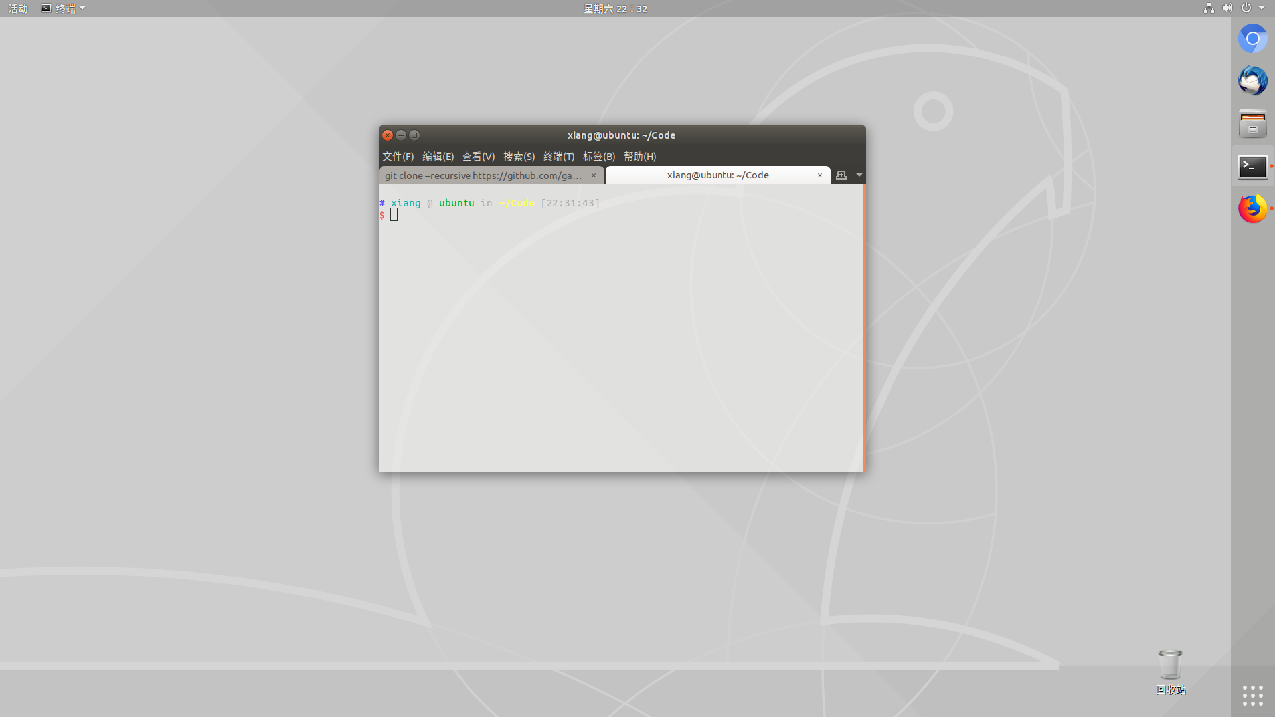
\includegraphics[width=0.8\textwidth]{whatIsSLAM/ubuntu1804.pdf}
	\caption{一个运行在虚拟机中的Ubuntu 18.04。}
	\label{fig:ubuntu1804}
\end{figure}

关于安装的小提示:
\begin{itemize}
	\item 安装操作系统时请不要选择“安装中下载更新”,并且断开网络连接,这样可以提高安装速度。至于更新可以在系统安装完毕后再装。如果你有SSD硬盘,这个过程大概用时15分钟。
	\item 安装完成后,请务必把软件源设置到离你较近的服务器上,以获得更快的下载速度。例如我使用清华的软件源通常能以10MB/s的速度安装软件\footnote{感谢TUNA同学们的维护!}。
\end{itemize}

现在,假设你已经成功安装好Ubuntu,无论是使用虚拟机还是双系统的方式。如果你还不熟悉Ubuntu,可以试试它的各种软件,体验一下它的界面和交互方式\footnote{大多数人第一次看到Ubuntu都觉得很漂亮。}。不过我必须\textbf{提醒}你,特别是新手朋友:不要在Ubuntu的用户界面上花费太多时间!Linux有许多可能浪费时间的地方,你可能会找到某些小众的软件、一些游戏,甚至会为找一张壁纸花费不少时间。但是请记住,你是用Linux来工作的。特别是在本书中,你是用Linux来学习SLAM的,所以要尽量把时间花在学习SLAM上。

好了,我们选择一个目录,放置本书中SLAM程序的代码。例如,可以将代码放到家目录(/home)的“slambook2”下。以后我们将把这个目录称为“\textbf{代码根目录}”。同时,可以另外选择一个目录,把本书的Git代码复制下来,方便做实验时随时对照。本书的代码是按章节划分的。比如,本讲的代码将在slambook2/ch2下,下一讲则在slambook2/ch3下。所以,现在请读者进入slambook2/ch2下(你应该会新建文件夹并进入该文件夹\mbox{了吧)。}

\subsection{Hello SLAM}
我们从最基本的程序开始。与许多计算机类书籍一样,我们来书写一个HelloSLAM程序。不过在做这件事之前,我们先来聊聊程序是什么。

在Linux中,程序是一个具有执行权限的文件。它可以是一个脚本,也可以是一个二进制文件,不过我们不限定它的后缀名(不像Windows那样需要指定成.exe文件)。我们常用的cd、ls等命令,就是位于/bin目录下的可执行文件。而对于其他地方的可执行程序,只要它有可执行权限,那么当我们在终端中输入程序名时,它就会运行。在C++编程时,我们先书写一个文本文件:

\begin{lstlisting}[language=C++,caption=slambook2/ch2/helloSLAM.cpp]
#include <iostream>
using namespace std;

int main(int argc, char **argv) {
	cout << "Hello SLAM!" << endl;
	return 0;
}
\end{lstlisting}

然后用一个叫做\textbf{编译器}的程序,把这个文本文件编译成可执行程序。显然这是一个非常简单的程序。你应该能毫不费力地看懂它,所以这里不多加解释——如果实际情况不是这样,请你先补习一下C++的基本知识。这个程序只是把一个字符串输出到屏幕上而已。你可以用文本编辑器gedit(或Vim,如果你在上一讲学习了Vim)输入这些代码,并保存在上面列出的路径下。现在,我们用编译器 g++ (g++是一个C++编译器)把它编译成一个可执行文件。输入:

\begin{lstlisting}[language=sh,caption=终端输入:]
g++ helloSLAM.cpp
\end{lstlisting}

如果顺利,这条命令应该没有任何输出。如果机器上出现“command not found”的错误信息,说明你可能还没有安装g++,请用如下命令进行安装:
\begin{lstlisting}[language=sh,caption=终端输入:]
sudo apt-get install g++
\end{lstlisting}
如果出现别的错误,请再检查一遍刚才的程序是否输入正确。

刚才这条编译命令把helloSLAM.cpp这个文本文件编译成了一个可执行程序。我们检查当前目录,会发现多了一个a.out文件,而且它具有执行权限(终端里颜色不同)。我们输入./a.out即可运行此程序\footnote{前头的\%为提示符,不要连这个也打进去。}:

\begin{lstlisting}[language=sh,caption=终端输入:]
% ./a.out
Hello SLAM!
\end{lstlisting}

如我们所想,这个程序输出“Hello SLAM!”,告诉我们它在正确运行。

请回顾一下我们之前做的事情。在这个例子中,我们用编辑器输入了helloSLAM.cpp的源代码,然后调用g++编译器对它进行编译,得到了可执行文件。g++默认把源文件编译成a.out这个名字的程序(虽然有些古怪,但是可以接受的)。如果我们愿意,也可以指定这个输出的文件名(留作习题)。这是一个极其简单的例子,我们\textbf{使用了大量的默认参数,几乎省略了所有中间步骤},为的是给读者一个简洁的印象(虽然你可能没有体会到)。下面我们要用cmake来编译这个程序。

\subsection{使用cmake}
理论上说,任意一个C++程序都可以用g++来编译。但当程序规模越来越大时,一个工程可能有许多个文件夹和源文件,这时输入的编译命令将越来越长。通常一个小型C++项目可能含有十几个类,各类间还存在着复杂的依赖关系。其中一部分要编译成可执行文件,另一部分编译成库文件。如果仅靠g++命令,我们需要输入大量的编译指令,整个编译过程会变得异常烦琐。因此,对于C++项目,使用一些工程管理工具会更加高效。在历史上工程师们曾使用makefile进行自动编译,但下面要谈的cmake比它更加方便。并且cmake在工程上广泛使用,我们会看到后面提到的大多数库都使用cmake来管理源代码。

在一个cmake工程中,我们会用cmake命令生成一个makefile文件,然后,用make命令根据这个makefile文件的内容编译整个工程。读者可能还不知道makefile是什么东西,不过没关系,我们会通过例子来学习。仍然以上面的helloSLAM.cpp为例,这次我们不是直接使用g++,而是用cmake来制作一个工程,然后再编译它。在slambook2/ch2/中新建一个CMakeLists.txt文件,内容如下:

%\clearpage
\begin{lstlisting}[language=Python,caption=slambook2/ch2/CMakeLists.txt]
# 声明要求的 cmake 最低版本
cmake_minimum_required( VERSION 2.8 )

# 声明一个 cmake 工程
project( HelloSLAM )

# 添加一个可执行程序
# 语法:add_executable( 程序名  源代码文件 )
add_executable( helloSLAM helloSLAM.cpp )
\end{lstlisting}

CMakeLists.txt文件用于告诉cmake我们要对这个目录下的文件做什么事情。CMakeLists.txt文件的内容需要遵守cmake的语法。这个示例中,我们演示了最基本的工程:指定一个工程名和一个可执行程序。根据注释,读者应该理解每句话做了些什么。

现在,在当前目录下(slambook2/ch2/),调用cmake对该工程进行cmake编译\footnote{指令最后有一个句点,请不要忘记,这表示在当前目录下进行cmake。}:

\begin{lstlisting}[language=sh,caption=终端输入:]
cmake .
\end{lstlisting}

cmake会输出一些编译信息,然后在当前目录下生成一些中间文件,其中最重要的就是MakeFile\footnote{MakeFile是一个自动化编译的脚本,读者现在可以将它理解成一系统自动生成的编译指令,而无须理会其内容。}。由于MakeFile是自动生成的,我们不必修改它。现在,用make命令对工程进行编译:
\begin{lstlisting}[language=sh,caption=终端输入:]
% make
Scanning dependencies of target helloSLAM
[100%] Building CXX object CMakeFiles/helloSLAM.dir/helloSLAM.cpp.o
Linking CXX executable helloSLAM
[100%] Built target helloSLAM
\end{lstlisting}

编译过程中会输出一个编译进度。如果顺利通过,我们就可以得到在CMakeLists.txt中声明的那个可执行程序helloSLAM。执行它:
\begin{lstlisting}[language=sh,caption=终端输入:]
% ./helloSLAM
Hello SLAM!
\end{lstlisting}

因为我们并没有修改源代码,所以得到的结果和之前是一样的。请读者想想这种做法和之前直接使用g++编译的区别。这次我们使用了先cmake再make的做法,cmake过程处理了工程文件之间的关系,而make过程实际调用了g++来编译程序。虽然这个过程中多了调用cmake和make的步骤,但我们对项目的编译管理工作,\textbf{从输入一串g++命令,变成了维护若干个比较直观的CMakeLists.txt文件},这将明显降低维护整个工程的难度。比如,如果想新增一个可执行文件,只需在CMakeLists.txt中添加一行“add\_executable”命令即可,而后续的步骤是不变的。cmake会帮我们解决代码的依赖关系,而无须输入一大串g++命令。

现在这个过程中唯一让我们不满的是,cmake生成的中间文件还留在我们的代码文件当中。当想要发布代码时,我们并不希望把这些中间文件一同发布出去。这时我们还需要把它们一个个删除,十分不便。一种更好的做法是让这些中间文件都放在一个中间目录中,在编译成功后,把这个中间目录删除即可。所以,更常见的编译cmake工程的做法如下:

\begin{lstlisting}[language=sh,caption=终端输入:]
mkdir build
cd build
cmake ..
make
\end{lstlisting}

我们新建了一个中间文件夹“build”,然后进入build文件夹,通过cmake ..命令对上一层文件夹,也就是代码所在的文件夹进行编译。这样,cmake产生的中间文件就会生成在build文件夹中,与源代码分开。当发布源代码时,只要把build文件夹删掉即可。请读者自行按照这种方式对ch2中的代码进行编译,然后调用生成的可执行程序(请记得把上一步产生的中间文件删掉)。

\subsection{使用库}
在一个C++工程中,并不是所有代码都会编译成可执行文件。只有带有main函数的文件才会生成可执行程序。而另一些代码,我们只想把它们打包成一个东西,供其他程序调用。这个东西叫作\textbf{库}(Library)。

一个库往往是许多算法、程序的集合,我们会在之后的练习中接触到许多库。例如,OpenCV库提供了许多计算机视觉相关的算法,而Eigen库提供了矩阵代数的计算。因此,我们要学习如何用cmake生成库,并且使用库中的函数。现在我们演示如何自己编写一个库。书写如下的libHelloSLAM.cpp文件:

\begin{lstlisting}[language=c++,caption=slambook2/ch2/libHelloSLAM.cpp]
//这是一个库文件
#include <iostream>
using namespace std;

void printHello() {
	cout << "Hello SLAM" << endl;
}
\end{lstlisting}

这个库提供了一个printHello函数,调用此函数将输出一条信息。但是它没有main函数,这意味着这个库中没有可执行文件。我们在CMakeLists.txt里加上如下内容:
\begin{lstlisting}[language=sh,caption=slambook2/ch2/CMakeLists.txt]
add_library( hello libHelloSLAM.cpp )
\end{lstlisting}

这条命令告诉cmake,我们想把这个文件编译成一个叫作“hello”的库。然后,和上面一样,使用cmake编译整个工程:
\begin{lstlisting}[language=sh,caption=终端输入:]
cd build
cmake ..
make
\end{lstlisting}
这时,在build文件夹中就会生成一个libhello.a文件,这就是我们得到的库。

在Linux中,库文件分成\textbf{静态库}和\textbf{共享库}两种\footnote{你多半猜错了,它并不叫作动态库。}。静态库以.a作为后缀名,共享库以.so结尾。所有库都是一些函数打包后的集合,差别在于\textbf{静态库每次被调用都会生成一个副本,而共享库则只有一个副本},更省空间。如果想生成共享库而不是静态库,只需使用以下语句即可。
\begin{lstlisting}[language=sh,caption=slambook2/ch2/CMakeLists.txt]
add_library( hello_shared SHARED libHelloSLAM.cpp )
\end{lstlisting}
此时得到的文件就是libhello\_shared.so了。

库文件是一个压缩包,里面有编译好的二进制函数。不过,如果仅有.a或.so库文件,那么我们并不知道里面的函数到底是什么,调用的形式又是什么样。为了让别人(或者自己)使用这个库,我们需要提供一个\textbf{头文件},说明这些库里都有些什么。因此,对于库的使用者,\textbf{只要拿到了头文件和库文件,就可以调用这个库了}。下面编写libhello的头文件。

\begin{lstlisting}[language=c++,caption=slambook2/ch2/libHelloSLAM.h]
#ifndef LIBHELLOSLAM_H_
#define LIBHELLOSLAM_H_
// 上面的宏定义是为了防止重复引用这个头文件而引起的重定义错误

// 打印一句hello的函数
void printHello();

#endif
\end{lstlisting}

这样,根据这个文件和我们刚才编译得到的库文件,就可以使用printHello函数了。最后,我们写一个可执行程序来调用这个简单的函数:

\begin{lstlisting}[language=c++,caption=slambook2/ch2/useHello.cpp]
#include "libHelloSLAM.h"

// 使用 libHelloSLAM.h 中的 printHello() 函数
int main(int argc, char **argv) {
	printHello();
	return 0;
}
\end{lstlisting}

然后,在CMakeLists.txt中添加一个可执行程序的生成命令,\textbf{链接}到刚才使用的库上:
\begin{lstlisting}[caption=slambook2/ch2/CMakeLists.txt]
add_executable( useHello useHello.cpp )
target_link_libraries( useHello hello_shared )
\end{lstlisting}

通过这两行语句,useHello程序就能顺利使用hello\_shared库中的代码了。这个小例子演示了如何生成并调用一个库。请注意,对于他人提供的库,我们也可用同样的方式对它们进行调用,整合到自己的程序中。

除了已经演示的功能之外,cmake还有许多语法和选项,这里不一一列举。实际上cmake很像一个正常的编程语言,有变量,有条件控制语句,所以你也可以像学习编程一样来学习cmake。习题中包含了一些cmake的阅读材料,感兴趣的读者可自行阅读。现在,简单回顾一下我们之前做了哪些事:

\begin{enumerate}
	\item 首先,程序代码由头文件和源文件组成。
	\item 带有main函数的源文件编译成可执行程序,其他的编译成库文件。
	\item 如果可执行程序想调用库文件中的函数,它需要参考该库提供的头文件,以明白调用的格式。同时,要把可执行程序链接到库文件上。
\end{enumerate}

这几个步骤应该是简单清楚的,但实际操作中你可能会遇上一些问题。比如说,如果代码里引用了库的函数,但忘了把程序链接到库上,会发生什么呢?请试试把CMakeLists.txt中的链接部分去掉,看看会发生什么情况。你能看懂cmake报告的错误消息吗?

\subsection{使用IDE}
最后,我们来谈谈如何使用集成开发环境(Integrated Development Environment,IDE)。前面的编程完全可以用一个简单的文本编辑器来完成。然而,你可能需要在各个文件之间跳转,查询某个函数的声明和实现。当文件很多时,这仍然很烦琐。IDE为开发者提供了跳转、补全、断点调试等很多方便的功能,所以,我们建议读者选择一个IDE进行开发。

Linux下的IDE有很多种。虽然与Windows下的Visual Studio还有一些差距,不过支持C++开发的也有好几种,例如:Eclipse、Qt Creator、Code::Blocks、Clion、Visual Studio Code,等等。同样,我们不强制读者使用某种特定的IDE,而仅给出我们的建议。我们使用的是Kdevelop和Clion(见\autoref{fig:kdevelop}和\autoref{fig:clion})\footnote{不过最近Visual Studio Code日趋完善,本身又免费,在开发者中大受欢迎,你也不妨试试。}。其中Kdevelop是一个免费软件,位于Ubuntu的软件仓库中,意味着你可以用apt-get来安装它;而Clion则是收费软件,但持有学生邮箱可以免费使用一年。二者都是很好的C++开发环境,优点列举如下:

\begin{enumerate}
	\item 支持cmake工程。
	\item 对C++支持较好(包括11及之后的标准)。有高亮、跳转、补全等功能。能自动排版\mbox{代码。}
	\item 能方便地看到各个文件和目录树。
	\item 有一键编译、断点调试等功能。
\end{enumerate}

\begin{figure}[!ht]
	\centering
	\includegraphics[width=0.8\textwidth]{whatIsSLAM/kdevelop.pdf}
	\caption{Kdevelop界面。}
	\label{fig:kdevelop}
\end{figure}

基本上,它们都具备人们对IDE的正常功能要求,所以读者不妨尝试一下。下面我们稍微花一点篇幅介绍一下Kdevelop和clion。

\subsubsection{Kdevelop的使用}

Kdevelop原生支持cmake工程。具体做法是,在终端建立CMakeLists.txt后,用Kdevelop中的“工程$\rightarrow$打开/导入工程”打开CMakeLists.txt。软件会询问你几个问题,并且默认建立一个build文件夹,帮你调用刚才的cmake和make命令。只要按下快捷键F8,这些都可以自动完成。\autoref{fig:kdevelop}的下面部分就显示了编译信息。

我们把适应IDE的任务交给读者自己来完成。如果你是从Windows转过来的,会觉得它的界面与Visual C++或Visual Studio挺相似。请用Kdevelop打开刚才的工程然后进行编译,看看它输出什么信息。相信你会觉得比打开终端更方便一些。

不过,本节重点想讲的是如何在IDE中进行调试。在Windows下编程的同学多半会有在Visual Studio下断点调试的经历。不过在Linux中,默认的调试工具gdb只提供了文本界面,对新手来讲不太方便。有些IDE提供了断点调试功能(底层仍旧是gdb),Kdevelop就是其中之一。要使用Kdevelop的断点调试功能,你需要完成以下几件事:

\begin{enumerate}
	\item 在CMakeLists.txt中把工程调为Debug编译模式,同时不要使用优化选项(默认不使用)。
	\item 告诉Kdevelop你想运行哪个程序。如果有参数,也要配置它的参数和工作目录。
	\item 进入断点调试界面,就可以单步运行,看到中间变量的值了。
\end{enumerate}

%\clearpage

第一步,在CMakeLists.txt中加入下面的命令来设置编译模式:
\begin{lstlisting}[caption=slambook2/ch2/CMakeLists.txt]
set( CMAKE_BUILD_TYPE "Debug" )
\end{lstlisting}

cmake自带一些编译相关的内部变量,它们可以对编译过程进行更精细的控制。对于编译类型,通常有调试用的Debug模式与发布用的Release模式。在Debug模式中,程序运行较慢,但可以进行断点调试;而Release模式则速度较快,但没有调试信息。我们把程序设置成Debug模式,就能放置断点了。接下来,告诉Kdevelop你想启动哪个程序。

第二步,打开“运行$\rightarrow$配置启动器”,然后单击左侧的“Add New$\rightarrow$应用程序”。在这一步中,我们的任务是告诉Kdevelop想要启动哪一个程序。如\autoref{fig:launchConfigure}所示,既可以选择一个cmake的工程目标(也就是我们用add_executable指令构建的可执行程序),也可以直接指向一个二进制文件。建议使用第二种方式,根据我们的经验,这样更少出现问题。

\begin{figure}[!ht]
	\centering
	\includegraphics[width=0.8\textwidth]{whatIsSLAM/launchConfigure.pdf}
	\caption{启动器设置界面。}
	\label{fig:launchConfigure}
\end{figure}

在第二栏里,可以设置程序的运行参数和工作目录。有时程序是有运行参数的,它们会作为main函数的参数被传入。如果没有则可以留空,对于工作目录亦是如此。配置好这两项后,单击“OK”按钮保存配置结果。

刚才这几步我们配置了一个应用程序的启动项。对于每一个启动项,我们可以单击“Execute”按钮直接启动这个程序,也可单击“Debug”按钮对它进行断点调试。读者可以试着单击“Execute”按钮,查看输出的结果。现在,为了调试这个程序,单击printHello那行的左侧,增加一个断点。然后,单击“Debug”按钮,程序会停留在断点处等待,如\autoref{fig:debug}所示。

\begin{figure}[!htp]
	\centering
	\includegraphics[width=0.8\textwidth]{whatIsSLAM/debug.pdf}
	\caption{调试界面。}
	\label{fig:debug}
\end{figure}

调试时,Kdevelop会切换到调试模式,界面会发生一点变化。在断点处,可以用单步运行(F10键)、单步跟进(F11键)、单步跳出(F12键)功能控制程序的运行。同时,可以点开左侧的界面,查看局部变量的值。或者选择“停止”按钮,结束调试。调试结束后,Kdevelop会回到正常的开发界面。

现在你应该熟悉了整个断点调试的流程。今后,如果在程序运行阶段发生了错误,导致程序崩溃,就可以用断点调试确定出错的位置,然后加以修正\footnote{而不是直接给我们发邮件询问怎么处理遇到的问题。}。

\subsubsection{Clion的使用}
\begin{figure}[!t]
	\centering
	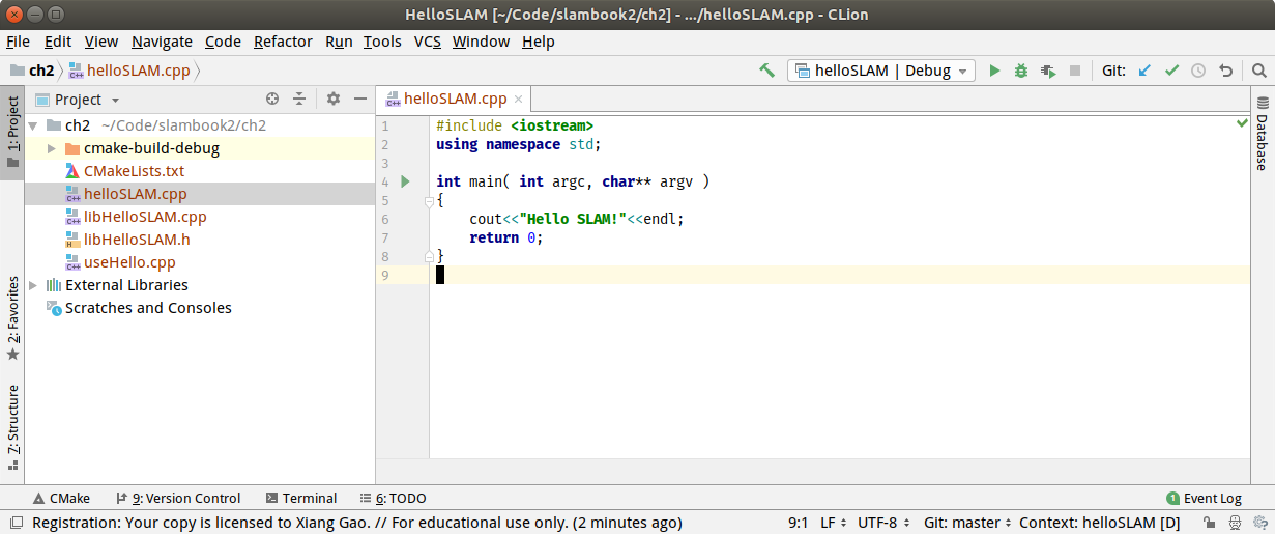
\includegraphics[width=1.0\textwidth]{whatIsSLAM/clion.pdf}
	\caption{Clion运行界面}
	\label{fig:clion}
\end{figure}
Clion相比于Kdevelop来说更加完善一些,但是它需要正版帐号,同时对主机的要求也会高一些\footnote{CLion在2018年之后的版本异常卡顿,推荐你用2017年左右的发布版。}。在Clion中,你同样可以打开一个CMakeLists.txt,或者指定目录。Clion会替你完成cmake-make的过程。它的运行界面如\autoref{fig:clion}所示。

同样的,在打开Clion之后,可以在界面右上角处选择你想运行或调试的程序,调整它们的启动参数和工作目录。点击该栏的小甲虫按钮可以启动断点调试模式。Clion还有许多方便的功能,比如自动创建类、函数改名、自动调整编码风格等,请一定要试一试。

好了,如果你已经熟悉了IDE的使用,那么入门章节也就到此为止。你或许已经觉得我有些话唠了,所以在今后的实践部分中,我们不会再介绍怎么新建build文件夹,调用cmake和make命令来编译程序。我相信读者应该掌握了这些简单的步骤。同样的,由于本书用到的大多第三方库都是cmake工程,你也会不断熟悉这个编译过程。接下来我们就开始正式的章节,介绍一些相关的数学知识。

\section*{习题}
\begin{enumerate}
	\item 阅读文献\cite{Liu2016}和\cite{Liang2013},你能看懂其中的内容吗?
	\item[\optional] 阅读SLAM的综述文献,例如\cite{Cadena2016, Fuentes-Pacheco2015, Boal2014, Chen2012, Chen2007}等。这些文献关于SLAM的看法与本书有何异同?
	\item g++命令有哪些参数?怎么填写参数可以更改生成的程序文件名?
	\item 使用build文件夹来编译你的cmake工程,然后在Kdevelop中试试。
	\item 刻意在代码中添加一些语法错误,看看编译会生成什么样的信息。你能看懂g++的错误信息吗?
	\item 如果忘了把库链接到可执行程序上,编译会报错吗?报什么样的错?
	\item[\optional] 阅读《cmake实践》,了解cmake的其他语法。
	\item[\optional] 完善hello SLAM小程序,把它做成一个小程序库,安装到本地硬盘中。然后,新建一个工程,使用find\_package找这个库并调用。
	\item[\optional] 阅读其他cmake教学材料,例如\url{https://github.com/TheErk/CMake-tutorial}。
	\item 找到Kdevelop的官方网站,看看它还有哪些特性。你都用上了吗?
	\item 如果在上一讲学习了Vim,请试试Kdevelop的Vim编辑功能。
\end{enumerate}
% ch3 三维刚体运动
% !Mode:: "TeX:UTF-8"
% 第二版:增加一个坐标变换的例子
\chapter{三维空间刚体运动}
\label{cpt:3}
\begin{mdframed}  
	\textbf{主要目标}
	\begin{enumerate}[labelindent=0em,leftmargin=1.5em]
		\item 理解三维空间的刚体运动描述方式:旋转矩阵、变换矩阵、四元数和欧拉角。
		\item 掌握Eigen库的矩阵、几何模块使用方法。
	\end{enumerate}
\end{mdframed} 

在上一讲中,我们讲解了视觉SLAM的框架与内容。本讲将介绍视觉SLAM的基本问题之一:\textbf{如何描述刚体在三维空间中的运动}?直观上看,我们当然知道这由一次旋转加一次平移组成。平移确实没有太大问题,但旋转的处理是件麻烦事。我们将介绍旋转矩阵、四元数、欧拉角的意义,以及它们是如何运算和转换的。在实践部分,我们将介绍线性代数库Eigen。它提供了C++中的矩阵运算,并且它的Geometry模块还提供了四元数等描述刚体运动的结构。Eigen的优化非常完善,但是它的使用方法有一些特殊的地方,我们留到程序中介绍。

\newpage
\includepdf{resources/other/ch3.pdf}

\newpage

\section{旋转矩阵}
\label{sec:rigidMotion}
\subsection{点和向量,坐标系}
我们日常生活的空间是三维的,因此我们生来就习惯于三维空间的运动。三维空间由3个轴组成,所以一个空间点的位置可以由3个坐标指定。不过,我们现在要考虑\textbf{刚体},它不光有位置,还有自身的姿态。相机也可以看成三维空间的刚体,于是位置是指相机在空间中的哪个地方,而姿态则是指相机的朝向。结合起来,我们可以说,“相机正处于空间$(0,0,0)$点处,朝向正前方”这样的话。但是这种自然语言很烦琐,我们更喜欢用数学语言来描述它。

我们从最基本的内容讲起:\textbf{点}和\textbf{向量}。点就是空间当中的基本元素,没有长度,没有体积。把两个点连接起来,就构成了向量。向量可以看成从某点指向另一点的一个箭头。需要提醒读者的是,请不要把向量与它的\textbf{坐标}两个概念混淆。一个向量是空间当中的一样东西,比如说$\bm{a}$。这里$\bm{a}$并不需要和若干个实数相关联的。只有当我们指定这个三维空间中的某个\textbf{坐标系}时,才可以谈论该向量在此坐标系下的坐标,也就是找到若干个实数对应这个向量。

用线性代数的知识来说,三维空间中的某个点的坐标也可以用$\mathbb{R}^3$来描述。怎么描述呢?假设在这个线性空间内,我们找到了该空间的一组\textbf{基}\footnote{以防读者忘记,基就是张成这个空间的一组线性无关的向量,有些书里也叫\textbf{基底}。}$(\bm{e}_1,\bm{e}_2,\bm{e}_3)$,那么,任意向量$\bm{a}$在这组基下就有一个\textbf{坐标}:
\begin{equation}
\bm{a} = \left[ {{\bm{e}_1},{\bm{e}_2},{\bm{e}_3}} \right]\left[ \begin{array}{l}
{a_1}\\
{a_2}\\
{a_3}
\end{array} \right] = {a_1}{\bm{e}_1} + {a_2}{\bm{e}_2} + {a_3}{\bm{e}_3}.
\end{equation}
这里$(a_1,a_2,a_3)^\mathrm{T}$称为$\bm{a}$在此基下的坐标\footnote{本书的向量为列向量,这和一般的数学书籍类似。}。坐标的具体取值,一是和向量本身有关,二是和坐标系(基)的选取有关。坐标系通常由3个正交的坐标轴组成(尽管也可以有非正交的,但实际中很少见)。例如,给定$\bm{x}$和$\bm{y}$轴时,$\bm{z}$轴就可以通过右手(或左手)法则由$\bm{x} \times \bm{y}$定义出来。根据定义方式的不同,坐标系又分为左手系和右手系。左手系的第3个轴与右手系方向相反。大部分3D程序库使用右手系(如OpenGL,3D Max等),也有部分库使用左手系(如Unity,Direct3D等)。

根据基本的线性代数知识,我们可以谈论向量与向量,以及向量与数之间的运算,例如数乘、加法、减法、内积、外积等。数乘和加减法都是相当基本的内容,也符合直观想象。例如,两个向量相加的结果就是把它们各自坐标相加,减法亦然,等等。这里不再赘述。内外积对读者来说可能有些陌生,这里给出它们的运算方式。对于$\bm{a}, \bm{b} \in \mathbb{R}^3$,通常意义下\footnote{内积也有形式化的法则,但本书只讨论通常的内积。}的内积可以写成:
\begin{equation}
\bm{a} \cdot \bm{b} = { \bm{a}^\mathrm{T}}\bm{b} = \sum\limits_{i = 1}^3 {{a_i}{b_i}}  = \left| \bm{a} \right|\left| \bm{b} \right|\cos \left\langle {\bm{a},\bm{b}} \right\rangle .
\end{equation}
其中$\left\langle {\bm{a},\bm{b}} \right\rangle$指向量$\bm{a},\bm{b}$的夹角。内积也可以描述向量间的投影关系。而外积则是这个样子:
\begin{equation}
\label{eq:cross}
\bm{a} \times \bm{b} = \left\| {\begin{array}{*{20}{c}}
	\bm{e}_1 & \bm{e}_2 & \bm{e}_3 \\
	{{a_1}}&{{a_2}}&{{a_3}}\\
	{{b_1}}&{{b_2}}&{{b_3}}
	\end{array}} \right\| = \left[ \begin{array}{l}
{a_2}{b_3} - {a_3}{b_2}\\
{a_3}{b_1} - {a_1}{b_3}\\
{a_1}{b_2} - {a_2}{b_1}
\end{array} \right] = \left[ {\begin{array}{*{20}{c}}
	0&{ - {a_3}}&{{a_2}}\\
	{{a_3}}&0&{ - {a_1}}\\
	{ - {a_2}}&{{a_1}}&0
	\end{array}} \right] \bm{b} \buildrel \Delta \over = { \bm{a}^ \wedge } \bm{b}.
\end{equation}

外积的结果是一个向量,它的方向垂直于这两个向量,大小为 $\left| \bm{a} \right|\left| \bm{b} \right|\sin \left\langle {\bm{a},\bm{b}} \right\rangle $,是两个向量张成的四边形的有向面积。对于外积运算,我们引入$^ \wedge$符号,把$\bm{a}$写成一个矩阵。事实上是一个\textbf{反对称矩阵}(Skew-symmetric matrix)\footnote{反对称矩阵$\bm{A}$满足$\bm{A}^\mathrm{T}=-\bm{A}$。},你可以将$^ \wedge$记成一个反对称符号。这样就把外积$\bm{a} \times \bm{b}$写成了矩阵与向量的乘法${ \bm{a}^ \wedge } \bm{b}$,把它变成了线性运算。这个符号将在后文经常用到,请记住它,并且此符号是一个一一映射,意味着任意向量都对应着唯一的一个反对称矩阵,反之亦然:
\begin{equation}
\bm{a}^\wedge = \left[ {\begin{array}{*{20}{c}}
	0&{ - {a_3}}&{{a_2}}\\
	{{a_3}}&0&{ - {a_1}}\\
	{ - {a_2}}&{{a_1}}&0
	\end{array}} \right].
\end{equation}

同时,需要提醒读者的是,向量和加减法、内外积,即使在不谈论它们的坐标时也可以计算。例如,虽然内积在有坐标时,可以用两个向量的分量乘积之和表达,但是即使不知道它们的坐标时,也可以通过长度和夹角来计算二者的内积。所以两个向量的内积结果和坐标系的选取是无关的。

%我们还能用外积表示向量的\textbf{旋转}。
%
%为什么外积可以表示旋转呢?
%
%考虑两个不平行的向量$\bm{a}, \bm{b}$,我们要描述从$\bm{a}$到$\bm{b}$之间是如何旋转的,如\autoref{fig:rotationOfVector}所示。我们可以用一个向量来描述三维空间中两个向量的旋转关系。在右手法则下,我们用右手的4个指头从$\bm{a}$转向$\bm{b}$,大拇指朝向就是旋转向量的方向,事实上也是$\bm{a} \times \bm{b}$的方向。它的大小则由$\bm{a}$和$\bm{b}$的夹角决定。通过这种方式,我们构造了从$\bm{a}$到$\bm{b}$的一个旋转向量。这个向量同样位于三维空间中,在此坐标系下,可以用3个实数来描述。
%
%\begin{figure}[!htp]
%	\centering
%	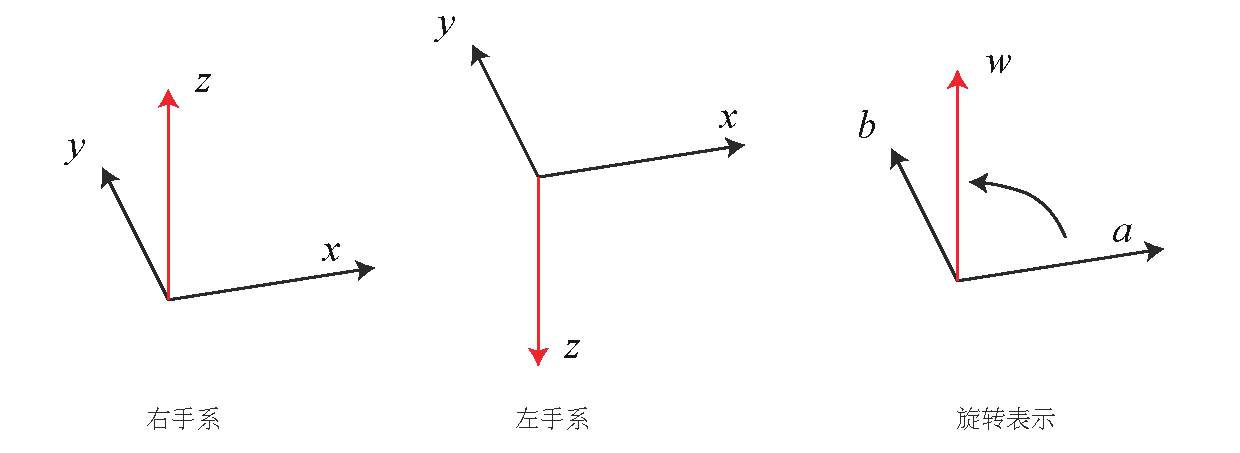
\includegraphics[width=1.0\textwidth]{rigidMotion/axis.pdf}
%	\caption{左右手系的区别与向量间的旋转。$\bm{a}$到$\bm{b}$的旋转可以由向量$\bm{w}$来描述。}
%	\label{fig:rotationOfVector}
%\end{figure}

\subsection{坐标系间的欧氏变换}
我们经常会在实际场景中定义各种各样的坐标系。在机器人学中,你会给每一个连杆和关节都定义它们的坐标系;在3D作图时,我们也会定义每一个长方体、圆柱体的坐标系。如果考虑运动的机器人,那么常见的做法是设定一个惯性坐标系(或者叫世界坐标系),可以认为它是固定不动的,例如\autoref{fig:axisTransform}中的$x_W, y_W, z_W$定义的坐标系。同时,相机或机器人则是一个移动坐标系,例如$x_C, y_C, z_C$定义的坐标系。我们可能会问:相机视野中某个向量$\bm{p}$,它在相机坐标系下的坐标为$\bm{p}_c$,而在世界坐标系下看,它的坐标为$\bm{p}_w$,那么,这两个坐标之间是如何转换的呢?这时,就需要先得到该点针对机器人坐标系的坐标值,再根据机器人位姿\textbf{变换}到世界坐标系中。我们需要一种数学手段来描述这个变换关系,稍后我们会看到,可以用一个矩阵$\bm{T}$来描述它。

\begin{figure}[!htp]
	\centering
	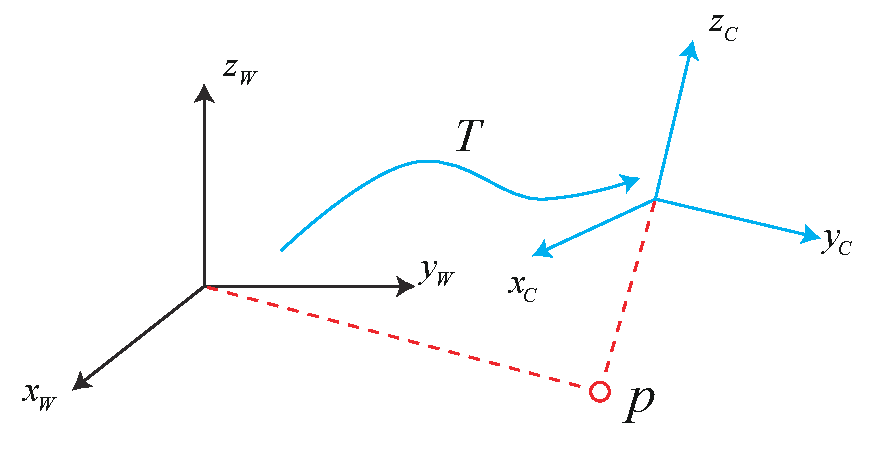
\includegraphics[width=0.7\textwidth]{rigidMotion/axisTransform.pdf}
	\caption{坐标变换。对于同一个向量$\bm{p}$,它在世界坐标系下的坐标$\bm{p}_w$和在相机坐标系下的坐标$\bm{p}_c$是不同的。这个变换关系由变换矩阵$\bm{T}$来描述。}
	\label{fig:axisTransform}
\end{figure}

直观上看,两个坐标系之间的运动由一个旋转加上一个平移组成,这种运动称为\textbf{刚体运动}。相机运动就是一个刚体运动。刚体运动过程中,同一个向量在各个坐标系下的长度和夹角都不会发生变化。想象你把手机抛到空中,在它落地摔碎之前\footnote{请不要付诸实践。},只可能有空间位置和姿态的不同,而它自己的长度、各个面的角度等性质不会有任何变化。手机并不会像橡皮那样一会儿被挤扁,一会儿被拉长。此时,我们说手机坐标系到世界坐标之间,相差了一个\textbf{欧氏变换}(Euclidean Transform)。

欧氏变换由旋转和平移组成。我们首先考虑旋转。设某个单位正交基$(\bm{e}_1,\bm{e}_2,\bm{e}_3)$经过一次旋转变成了$(\bm{e}_1', \bm{e}_2', \bm{e}_3')$。那么,对于同一个向量$\bm{a}$(该向量并没有随着坐标系的旋转而发生运动),它在两个坐标系下的坐标为$[a_1,a_2,a_3]^\mathrm{T}$和$[a'_1, a'_2, a'_3]^\mathrm{T}$。因为向量本身没变,根据坐标的定义,有:

\begin{equation}
\left[ \bm{e}_1,\bm{e}_2,\bm{e}_3 \right]\left[ \begin{array}{l}
{a_1}\\
{a_2}\\
{a_3}
\end{array} \right] = \left[ \bm{e}_1', \bm{e}_2', \bm{e}_3' \right]\left[ \begin{array}{l}
a'_1\\
a'_2\\
a'_3
\end{array} \right].
\end{equation}

为了描述两个坐标之间的关系,我们对上述等式的左右两边同时左乘$\left[ \begin{array}{l}
\bm{e}_1^\mathrm{T}\\
\bm{e}_2^\mathrm{T}\\
\bm{e}_3^\mathrm{T}
\end{array} \right]$,那么左边的系数就变成了单位矩阵,所以:
%\clearpage
\begin{equation}
\left[ \begin{array}{l}
{a_1}\\
{a_2}\\
{a_3}
\end{array} \right] = \left[ {\begin{array}{*{20}{c}}
	{\bm{e}_1^\mathrm{T}\bm{e}_1'} & {\bm{e}_1^\mathrm{T}\bm{e}_2'} & {\bm{e}_1^\mathrm{T}\bm{e}_3'}\\
	{\bm{e}_2^\mathrm{T}\bm{e}_1'} & {\bm{e}_2^\mathrm{T}\bm{e}_2'} & {\bm{e}_2^\mathrm{T}\bm{e}_3'}\\
	{\bm{e}_3^\mathrm{T}\bm{e}_1'} & {\bm{e}_3^\mathrm{T}\bm{e}_2'} & {\bm{e}_3^\mathrm{T}\bm{e}_3'}
	\end{array}} \right]\left[ \begin{array}{l}
a_1'\\
a_2'\\
a_3'
\end{array} \right] \buildrel \Delta \over = \bm{R} \bm{a}'.
\end{equation}
我们把中间的矩阵拿出来,定义成一个矩阵$\bm{R}$。这个矩阵由两组基之间的内积组成,刻画了旋转前后同一个向量的坐标变换关系。只要旋转是一样的,那么这个矩阵也是一样的。可以说,矩阵$\bm{R}$描述了旋转本身。因此称为\textbf{旋转矩阵}(Rotation matrix)。同时,该矩阵各分量是两个坐标系基的内积,由于基向量的长度为1,所以实际上是各基向量的夹角之余弦。所以这个矩阵也叫\textbf{方向余弦矩阵}(Direction Cosine matrix)。我们后文统一称呼它为旋转矩阵。

旋转矩阵有一些特别的性质。事实上,它是一个行列式为1的正交矩阵\footnote{正交矩阵即逆为自身转置的矩阵。旋转矩阵的正交性可以直接由定义得出。}\footnote{行列式为1是人为定义的,实际上只要求它的行列式为$\pm 1$,但行列式为$-1$的称为瑕旋转,即一次旋转加一次反射。}。反之,行列式为1的正交矩阵也是一个旋转矩阵。所以,可以把$n$维旋转矩阵的集合定义如下:
\begin{equation}
\mathrm{SO}(n) = \{ \bm{R} \in \mathbb{R}^{n \times n} | \bm{R R}^\mathrm{T} = \bm{I}, \mathrm{det} (\bm{R})=1 \}.
\end{equation}

$\mathrm{SO}(n)$是\textbf{特殊正交群}(Special Orthogonal Group)的意思。我们把“群”的内容留到下一讲。这个集合由$n$维空间的旋转矩阵组成,特别地,$\mathrm{SO}(3)$就是指三维空间的旋转。通过旋转矩阵,我们可以直接谈论两个坐标系之间的旋转变换,而不用再从基开始谈起。

由于旋转矩阵为正交矩阵,它的逆(即转置)描述了一个相反的旋转。按照上面的定义方式,有:
\begin{equation}
\bm{a}' = \bm{R}^{-1} \bm{a} =\bm{R}^\mathrm{T} \bm{a} .
\end{equation}
显然$\bm{R}^\mathrm{T}$刻画了一个相反的旋转。

在欧氏变换中,除了旋转之外还有平移。考虑世界坐标系中的向量$\bm{a}$,经过一次旋转(用$\bm{R}$描述)和一次平移$\bm{t}$后,得到了$\bm{a}'$,那么把旋转和平移合到一起,有:
\begin{equation}
\label{eq:RT}
\bm{a}' = \bm{R} \bm{a} + \bm{t}.
\end{equation}
其中,$\bm{t}$称为平移向量。相比于旋转,平移部分只需把平移向量加到旋转之后的坐标上,非常简单。通过上式,我们用一个旋转矩阵$\bm{R}$和一个平移向量$\bm{t}$完整地描述了一个欧氏空间的坐标变换关系。实际当中,我们会定义坐标系1、坐标系2,那么向量$\bm{a}$在两个系下坐标为$\bm{a}_1, \bm{a}_2$,它们之间的关系,按照完整的写法,应该是:
\begin{equation}
\bm{a}_1 = \bm{R}_{12} \bm{a}_2 + \bm{t}_{12}.
\end{equation}
这里的$\bm{R}_{12}$是指“把坐标系2的向量变换到坐标系1”中。由于向量乘在这个矩阵的右边,它的下标是\textbf{从右读到左}的。这也是本书的习惯写法。坐标变换很容易搞混,特别是存在多个坐标系的情况下。同理,如果我们要表达“从1到2的旋转矩阵”时,就写成$\bm{R}_{21}$。请读者务必清楚这边的记法,因为不同书籍里写法不同,有的会记成左上/下标,而本书写在右侧下标。

关于平移$\bm{t}_{12}$,它实际对应的是坐标系1原点指向坐标系2原点的向量,\textbf{在坐标系1下取的坐标},所以我建议读者把它记作“从1到2的向量”。但是反过来的$\bm{t}_{21}$,即从2指向1的向量\textbf{在坐标系2下的坐标},却并不等于$-\bm{t}_{12}$,而是和两个系的旋转还有关系\footnote{尽管从向量层面来看,它们确实是反向的关系,但这两个向量的坐标值并不是相反数。你能想清楚这是为什么吗?}。所以,当初学者问“我的坐标在哪里”这样的问题时,我们需要清楚地说明这句话的含义。这里“我的坐标”实际上指从世界坐标系指向自己坐标系原点的向量,在世界坐标系下取到的坐标。对应到数学符号上,应该是$\bm{t}_{WC}$的取值。同理,它也不是$-\bm{t}_{CW}$。

\subsection{变换矩阵与齐次坐标}

式\eqref{eq:RT}完整地表达了欧氏空间的旋转与平移,不过还存在一个小问题:这里的变换关系不是一个线性关系。假设我们进行了两次变换:$\bm{R}_1,\bm{t}_1$和$\bm{R}_2,\bm{t}_2$:

\[
\bm{b} = {\bm{R}_1} \bm{a} + {\bm{t}_1}, \quad \bm{c} = {\bm{R}_2} \bm{b} + {\bm{t}_2}.
\]
那么,从$\bm{a}$到$\bm{c}$的变换为:
\[
\bm{c} = {\bm{R}_2}\left( {{\bm{R}_1} \bm{a} + {\bm{t}_1}} \right) + {\bm{t}_2}.
\]
这样的形式在变换多次之后会显得很啰嗦。因此,我们引入齐次坐标和变换矩阵,重写式\eqref{eq:RT}:
\begin{equation}
\left[ \begin{array}{l}
\bm{a}'\\
1
\end{array} \right] = 
\left[ {\begin{array}{*{20}{c}}
	\bm{R}&\bm{t}\\
	{{\bm{0}^\mathrm{T}}}&1
	\end{array}} \right]
\left[ \begin{array}{l}
\bm{a}\\
1
\end{array} \right]  \buildrel \Delta \over = \bm{T} \left[ \begin{array}{l}
\bm{a}\\
1
\end{array} \right].
\end{equation}

这是一个数学技巧:我们在一个三维向量的末尾添加$1$,将其变成了四维向量,称为\textbf{齐次坐标}。对于这个四维向量,我们可以把旋转和平移写在一个矩阵里面,使得整个关系变成线性关系。该式中,矩阵$\bm{T}$称为\textbf{变换矩阵(Transform Matrix)}。
%
%稍微说一下齐次坐标。它是射影几何里的概念。通过添加最后一维,我们用4个实数描述了一个三维向量,这显然多了一个自由度,但允许我们把变换写成线性的形式。在齐次坐标中,某个点$\bm{x}$的每个分量同乘一个非零常数$k$后,\textbf{仍然表示同一个点}。因此,一个点的具体坐标值不是唯一的。如$\left[1,1,1,1\right]^\mathrm{T}$和$\left[2,2,2,2\right]^\mathrm{T}$是同一个点。但当最后一项不为零时,我们总可以把所有坐标除以最后一项,强制最后一项为1,从而得到一个点唯一的坐标表示(也就是转换成非齐次坐标):
%\begin{equation}
%\tilde{\bm{x}} = \left[ x, y, z,w \right]^\mathrm{T} = \left[ x/w, y/w, z/w, 1 \right]^\mathrm{T} .
%\end{equation}
%
%这时,忽略掉最后一项,这个点的坐标和欧氏空间就是一样的。

我们暂时用$ \tilde{ \bm{a} }$表示$\bm{a}$的齐次坐标。那么依靠齐次坐标和变换矩阵,两次变换的叠加就可以有很好的形式:
\begin{equation}
	\tilde{\bm{b}} = \bm{T}_1 \tilde{\bm{a}}, \  \tilde{\bm{c}} = \bm{T}_2 \tilde{\bm{b}} \quad \Rightarrow \tilde{\bm{c}} = \bm{T}_2 \bm{T_1} \tilde{\bm{a}}.
\end{equation}
但是区分齐次和非齐次坐标的符号令我们感到厌烦,因为此处只需要在向量末尾添加1或者去掉1即可\footnote{但齐次坐标的用途不止于此,我们在第7章还会再介绍。}。所以,在不引起歧义的情况下,以后我们就直接把它写成$\bm{b}= \bm{T} \bm{a}$的样子,默认其中进行了齐次坐标的转换\footnote{注意,不进行齐次坐标转换时,这边的乘法在矩阵维度上是不成立的。}。

关于变换矩阵$\bm{T}$,它具有比较特别的结构:左上角为旋转矩阵,右侧为平移向量,左下角为$\bm{0}$向量,右下角为1。这种矩阵又称为特殊欧氏群(Special Euclidean Group):
\begin{equation}
\mathrm{SE}(3) = \left\{ \bm{T} = \left[ {\begin{array}{*{20}{c}}
	\bm{R} & \bm{t} \\
	{{\bm{0}^\mathrm{T}}} & 1
	\end{array}} \right]
\in \mathbb{R}^{4 \times 4} | \bm{R} \in \mathrm{SO}(3), \bm{t} \in \mathbb{R}^3\right\} .
\end{equation}

与$\mathrm{SO}(3)$一样,求解该矩阵的逆表示一个反向的变换:
\begin{equation}
{ \bm{T}^{ - 1}} = \left[ {\begin{array}{*{20}{c}}
	{{\bm{R}^\mathrm{T}}}&{ - {\bm{R}^\mathrm{T}}\bm{t}}\\
	{{\bm{0}^\mathrm{T}}}&1
	\end{array}} \right].
\end{equation}

同样,我们用$\bm{T}_{12}$这样的写法来表示从2到1的变换。并且,为了保持符号的简洁,在不引起歧义的情况下,以后不刻意区别齐次坐标与普通坐标的符号,\textbf{默认使用的是符合运算法则的那一种}。例如,当我们写$\bm{T} \bm{a}$时,使用的是齐次坐标(不然没法计算)。而写$\bm{Ra}$时,使用的是非齐次坐标。如果写在一个等式中,就假设齐次坐标到普通坐标的转换,是已经做好了的——因为齐次坐标和非齐次坐标之间的转换事实上非常容易,而在C++程序中你可以使用\textbf{运算符重载}来完成这个功能,保证在程序中看到的运算是统一的。

回顾一下:首先,我们介绍了向量及其坐标表示,并介绍了向量间的运算;然后,坐标系之间的运动由欧氏变换描述,它由平移和旋转组成。旋转可以由旋转矩阵$\mathrm{SO}(3)$描述,而平移直接由一个$\mathbb{R}^3$向量描述。最后,如果将平移和旋转放在一个矩阵中,就形成了变换矩阵$\mathrm{SE}(3)$。

\section{实践:Eigen}
本讲的实践部分有两节。第一部分中,将讲解如何使用Eigen来表示矩阵、向量,随后引申至旋转矩阵与变换矩阵的计算。本节的代码在slambook2/ch3/useEigen中。

Eigen\footnote{官方主页:\url{http://eigen.tuxfamily.org/index.php?title=Main_Page}。}是一个C++开源线性代数库。它提供了快速的有关矩阵的线性代数运算,还包括解方程等功能。许多上层的软件库也使用Eigen进行矩阵运算,包括g2o、Sophus等。照应本讲的理论部分,我们来学习一下Eigen的编程。

你的PC上可能还没有安装Eigen。请输入以下命令进行安装:
\begin{lstlisting}[language=sh,caption=终端输入:]
sudo apt-get install libeigen3-dev
\end{lstlisting}

大部分常用的库都已在Ubuntu软件源中提供。以后,若想要安装某个库,不妨先搜索一下Ubuntu的软件源中是否已提供。通过apt命令,我们能够方便地安装Eigen。回顾上一讲的知识,我们知道一个库由头文件和库文件组成。Eigen头文件的默认位置在“/usr/include/eigen3/”中。如果不确定,可以输入以下命令查找:
\begin{lstlisting}[language=sh,caption=终端输入:]
sudo updatedb
locate eigen3
\end{lstlisting}
相比于其他库,Eigen的特殊之处在于,它是一个纯用头文件搭建起来的库(这非常神奇!)。这意味着你只能找到它的头文件,而没有.so或.a那样的二进制文件。在使用时,只需引入Eigen的头文件即可,不需要链接库文件(因为它没有库文件)。下面写一段代码来实际练习一下Eigen的使用:

\begin{lstlisting}[language=c++,caption=slambook2/ch3/useEigen/eigenMatrix.cpp]
#include <iostream>
using namespace std;

#include <ctime>
// Eigen 核心部分
#include <Eigen/Core>
// 稠密矩阵的代数运算(逆,特征值等)
#include <Eigen/Dense>
using namespace Eigen;

#define MATRIX_SIZE 50

/****************************
* 本程序演示了 Eigen 基本类型的使用
****************************/

int main(int argc, char **argv) {
	// Eigen 中所有向量和矩阵都是Eigen::Matrix,它是一个模板类。它的前三个参数为:数据类型,行,列
	// 声明一个2*3的float矩阵
	Matrix<float, 2, 3> matrix_23;
	
	// 同时,Eigen 通过 typedef 提供了许多内置类型,不过底层仍是Eigen::Matrix
	// 例如 Vector3d 实质上是 Eigen::Matrix<double, 3, 1>,即三维向量
	Vector3d v_3d;
	// 这是一样的
	Matrix<float, 3, 1> vd_3d;
	
	// Matrix3d 实质上是 Eigen::Matrix<double, 3, 3>
	Matrix3d matrix_33 = Matrix3d::Zero(); //初始化为零
	// 如果不确定矩阵大小,可以使用动态大小的矩阵
	Matrix<double, Dynamic, Dynamic> matrix_dynamic;
	// 更简单的
	MatrixXd matrix_x;
	// 这种类型还有很多,我们不一一列举
	
	// 下面是对Eigen阵的操作
	// 输入数据(初始化)
	matrix_23 << 1, 2, 3, 4, 5, 6;
	// 输出
	cout << "matrix 2x3 from 1 to 6: \n" << matrix_23 << endl;
	
	// 用()访问矩阵中的元素
	cout << "print matrix 2x3: " << endl;
	for (int i = 0; i < 2; i++) {
		for (int j = 0; j < 3; j++) cout << matrix_23(i, j) << "\t";
		cout << endl;
	}
	
	// 矩阵和向量相乘(实际上仍是矩阵和矩阵)
	v_3d << 3, 2, 1;
	vd_3d << 4, 5, 6;
	
	// 但是在Eigen里你不能混合两种不同类型的矩阵,像这样是错的
	// Matrix<double, 2, 1> result_wrong_type = matrix_23 * v_3d;
	// 应该显式转换
	Matrix<double, 2, 1> result = matrix_23.cast<double>() * v_3d;
	cout << "[1,2,3;4,5,6]*[3,2,1]=" << result.transpose() << endl;
	
	Matrix<float, 2, 1> result2 = matrix_23 * vd_3d;
	cout << "[1,2,3;4,5,6]*[4,5,6]: " << result2.transpose() << endl;
	
	// 同样你不能搞错矩阵的维度
	// 试着取消下面的注释,看看Eigen会报什么错
	// Eigen::Matrix<double, 2, 3> result_wrong_dimension = matrix_23.cast<double>() * v_3d;
	
	// 一些矩阵运算
	// 四则运算就不演示了,直接用+-*/即可。
	matrix_33 = Matrix3d::Random();      // 随机数矩阵
	cout << "random matrix: \n" << matrix_33 << endl;
	cout << "transpose: \n" << matrix_33.transpose() << endl; // 转置
	cout << "sum: " << matrix_33.sum() << endl;               // 各元素和
	cout << "trace: " << matrix_33.trace() << endl;           // 迹
	cout << "times 10: \n" << 10 * matrix_33 << endl;         // 数乘
	cout << "inverse: \n" << matrix_33.inverse() << endl;     // 逆
	cout << "det: " << matrix_33.determinant() << endl;       // 行列式
	
	// 特征值
	// 实对称矩阵可以保证对角化成功
	SelfAdjointEigenSolver<Matrix3d> eigen_solver(matrix_33.transpose() * matrix_33);
	cout << "Eigen values = \n" << eigen_solver.eigenvalues() << endl;
	cout << "Eigen vectors = \n" << eigen_solver.eigenvectors() << endl;
	
	// 解方程
	// 我们求解 matrix_NN * x = v_Nd 这个方程
	// N的大小在前边的宏里定义,它由随机数生成
	// 直接求逆自然是最直接的,但是求逆运算量大
	
	Matrix<double, MATRIX_SIZE, MATRIX_SIZE> matrix_NN
		= MatrixXd::Random(MATRIX_SIZE, MATRIX_SIZE);
	matrix_NN = matrix_NN * matrix_NN.transpose();  // 保证半正定
	Matrix<double, MATRIX_SIZE, 1> v_Nd = MatrixXd::Random(MATRIX_SIZE, 1);
	
	clock_t time_stt = clock(); // 计时
	// 直接求逆
	Matrix<double, MATRIX_SIZE, 1> x = matrix_NN.inverse() * v_Nd;
	cout << "time of normal inverse is "
	     << 1000 * (clock() - time_stt) / (double) CLOCKS_PER_SEC << "ms" << endl;
	cout << "x = " << x.transpose() << endl;
	
	// 通常用矩阵分解来求,例如QR分解,速度会快很多
	time_stt = clock();
	x = matrix_NN.colPivHouseholderQr().solve(v_Nd);
	cout << "time of Qr decomposition is "
	     << 1000 * (clock() - time_stt) / (double) CLOCKS_PER_SEC << "ms" << endl;
	cout << "x = " << x.transpose() << endl;
	
	// 对于正定矩阵,还可以用cholesky分解来解方程
	time_stt = clock();
	x = matrix_NN.ldlt().solve(v_Nd);
	cout << "time of ldlt decomposition is "
	     << 1000 * (clock() - time_stt) / (double) CLOCKS_PER_SEC << "ms" << endl;
	cout << "x = " << x.transpose() << endl;
	
	return 0;
}
\end{lstlisting}

这个例程演示了Eigen矩阵的基本操作与运算。要编译它,需要在CMakeLists.txt里指定Eigen的头文件目录:
\begin{lstlisting}[caption=slambook2/ch3/useEigen/CMakeLists.txt]
# 添加头文件
include_directories( "/usr/include/eigen3" )
\end{lstlisting}

重复一遍,因为Eigen库只有头文件,所以不需要再用target\_link\_libraries语句将程序链接到库上。不过,对于其他大部分库,多数时候需要用到链接命令。这里的做法并不见得是最好的,因为其他人可能把Eigen安装在了不同位置,那么就必须手动修改这里的头文件目录。在之后的工作中,我们会使用find\_package命令去搜索库,不过在本讲中暂时保持这个样子。编译好这个程序后,运行它,可以看到各矩阵的输出结果。

\begin{lstlisting}[caption=终端输入:]
% build/eigenMatrix
matrix 2x3 from 1 to 6: 
1 2 3
4 5 6
print matrix 2x3: 
1	2	3	
4	5	6	
[1,2,3;4,5,6]*[3,2,1]=10 28
[1,2,3;4,5,6]*[4,5,6]: 32 77
random matrix: 
0.680375   0.59688 -0.329554
-0.211234  0.823295  0.536459
0.566198 -0.604897 -0.444451
transpose: 
0.680375 -0.211234  0.566198
0.59688  0.823295 -0.604897
-0.329554  0.536459 -0.444451
sum: 1.61307
trace: 1.05922
times 10: 
6.80375   5.9688 -3.29554
-2.11234  8.23295  5.36459
5.66198 -6.04897 -4.44451
inverse: 
-0.198521   2.22739    2.8357
1.00605 -0.555135  -1.41603
-1.62213   3.59308   3.28973
det: 0.208598
……
\end{lstlisting}

由于在代码中给出了详细的注释,在此就不一一解释每行语句了。本书中,我们将仅给出几处重要地方的说明(后面的实践部分亦将保持这个风格)。

\begin{enumerate}
	\item 读者最好亲手输入一遍上面的代码(不包括注释)。至少要编译运行一遍上面的程序。
	
	\item Kdevelop可能不会提示C++成员运算,这是它做得不够完善导致的。请照着上面的内容输入即可,不必理会它是否提示错误。Clion则会完整地给出提示。
	
	\item Eigen提供的矩阵和MATLAB很相似,几乎所有的数据都当作矩阵来处理。但是,为了实现更好的效率,在Eigen中需要指定矩阵的大小和类型。对于在编译时期就知道大小的矩阵,处理起来会比动态变化大小的矩阵更快一些。因此,像旋转矩阵、变换矩阵这样的数据,完全可在编译时期确定它们的大小和数据类型。
	
	\item Eigen内部的矩阵实现比较复杂,这里不做介绍,我们希望你像使用float、double等内置数据类型那样使用Eigen的矩阵。这应该是符合其设计初衷的。
	
	\item Eigen矩阵不支持自动类型提升,这和C++的内建数据类型有较大差异。在C++程序中,我们可以把一个float数据和double数据相加、相乘,\textbf{编译器会自动把数据类型转换为最合适的那种}。而在Eigen中,出于性能的考虑,必须\textbf{显式地}对矩阵类型进行转换。而如果忘了这样做,Eigen会(不太友好地)提示你一个“YOU MIXED DIFFERENT NUMERIC TYPES ...”的编译错误。你可以尝试找一下这条信息出现在错误提示的哪个部分。如果错误信息太长最好保存到一个文件里再找。
	
	\item 同理,在计算过程中也需要保证矩阵维数的正确性,否则会出现“YOU MIXED MATRICES OF DIFFERENT SIZES”错误。请不要抱怨这种错误提示方式,对于C++模板元编程,能够提示出可以阅读的信息已经是很幸运的了。以后,若发现Eigen出错,你可以直接寻找大写的部分,推测出了什么问题。
	
	\item 我们的例程只介绍了基本的矩阵运算。你可以阅读Eigen官网教程:\\{\url{http://eigen.tuxfamily.org/dox-devel/modules.html}}学习更多的Eigen知识。这里只演示了最简单的部分,能看懂演示程序不等于你已经能够熟练操作Eigen。
\end{enumerate}

最后一段代码中比较了求逆与求QR分解的运行效率,你可以看看自己机器上的时间差异,两种方法是否有明显的差异?

\section{旋转向量和欧拉角}
\subsection{旋转向量}
我们重新回到理论部分。有了旋转矩阵来描述旋转,有了变换矩阵描述一个6自由度的三维刚体运动,是不是已经足够了呢?矩阵表示方式至少有以下几个缺点:

\begin{enumerate}
	\item $\mathrm{SO}(3)$的旋转矩阵有9个量,但一次旋转只有3个自由度。因此这种表达方式是冗余的。同理,变换矩阵用16个量表达了6自由度的变换。那么,是否有更紧凑的表示呢?
	\item 旋转矩阵自身带有约束:它必须是个正交矩阵,且行列式为1。变换矩阵也是如此。当想要估计或优化一个旋转矩阵/变换矩阵时,这些约束会使得求解变得更困难。
\end{enumerate}

因此,我们希望有一种方式能够紧凑地描述旋转和平移。例如,用一个三维向量表达旋转,用六维向量表达变换,可行吗?事实上,任意旋转都可以用\textbf{一个旋转轴和一个旋转角}来刻画。于是,我们可以使用一个向量,其方向与旋转轴一致,而长度等于旋转角。这种向量称为\textbf{旋转向量}(或轴角/角轴,Axis-Angle),只需一个三维向量即可描述旋转。同样,对于变换矩阵,我们使用一个旋转向量和一个平移向量即可表达一次变换。这时的变量维数正好是六维。

考虑某个用$\bm{R}$表示的旋转。如果用旋转向量来描述,假设旋转轴为一个单位长度的向量$\bm{n}$,角度为$\theta$,那么向量$\theta \bm{n}$也可以描述这个旋转。于是,我们要问,两种表达方式之间有什么联系吗?事实上推导它们的转换关系并不难。从旋转向量到旋转矩阵的转换过程由\textbf{罗德里格斯公式}(Rodrigues' Formula )表明,由于推导过程比较复杂,这里不作描述,只给出转换的结果\footnote{感兴趣的读者请参见\url{https://en.wikipedia.org/wiki/Rodrigues\%27_rotation_formula},事实上下一章会从李代数层面给出一个证明。}:
\begin{equation}
\label{eq:rogridues}
\bm{R} = \cos \theta \bm{I} + \left( {1 - \cos \theta } \right) \bm{n}{\bm{n}^\mathrm{T}} + \sin \theta { \bm{n}^ \wedge }.
\end{equation}

符号$^\wedge$是向量到反对称的转换符,见式\eqref{eq:cross}。反之,我们也可以计算从一个旋转矩阵到旋转向量的转换。对于转角$\theta$,取两边的\textbf{迹}\footnote{求\textbf{迹}(trace)即是求矩阵的对角线元素之和。},有:
\begin{equation}
\begin{aligned}
  \mathrm{tr} \left( \bm{R} \right) &= \cos \theta \mathop{}\!\mathrm{tr}\left( \bm{I} \right) + \left( {1 - \cos \theta } \right) \mathop{}\!\mathrm{tr} \left( { \bm{n} {\bm{n}^\mathrm{T}}} \right) + \sin \theta \mathop{}\!\mathrm{tr} ({\bm{n}^ \wedge })\\
&= 3\cos \theta  + (1 - \cos \theta )\\
&= 1 + 2\cos \theta .
\end{aligned} 
\end{equation}

因此:
\begin{equation}
\label{eq:R2theta}
\theta = \arccos ( \frac{\mathrm{tr}(\bm{R}) - 1}{2}  ) .
\end{equation}

关于转轴$\bm{n}$,由于旋转轴上的向量在旋转后不发生改变,说明:
\begin{equation}
\bm{R} \bm{n} = \bm{n}.	
\end{equation}

因此,转轴$\bm{n}$是矩阵$\bm{R}$特征值1对应的特征向量。求解此方程,再归一化,就得到了旋转轴。读者也可以从“旋转轴经过旋转之后不变”的几何角度看待这个方程。顺便提一下,这里的两个转换公式在下一讲仍将出现,你会发现它们正是$\mathrm{SO}(3)$上李群与李代数的对应关系。

\subsection{欧拉角}
下面来说说欧拉角。

无论是旋转矩阵、旋转向量,它们虽然能描述旋转,但对我们人类是非常不直观的。当我们看到一个旋转矩阵或旋转向量时,很难想象出这个旋转究竟是什么样的。当它们变换时,我们也不知道物体是向哪个方向在转动。而欧拉角则提供了一种非常直观的方式来描述旋转——它使用了\textbf{3个分离的转角},把一个旋转分解成3次绕不同轴的旋转。而人类很容易理解绕单个轴旋转的过程。但是,由于分解方式有许多种,所以欧拉角也存在着众多不同的、易于混淆的定义方法。比如说,先绕$X$轴旋转,再绕$Y$轴,最后绕$Z$轴,就得到了一个$XYZ$轴的旋转。同理,可以定义$ZYZ$、$ZYX$等旋转方式。如果讨论得更细一些,还需要区分每次是绕\textbf{固定轴}旋转的,还是绕\textbf{旋转之后的轴}旋转的,这也会给出不一样的定义方式。

这种定义方式上的不确定性带来了很多实用当中的困难,所幸在特定领域内,欧拉角通常有统一的定义方式。你或许在航空、航模中听说过“俯仰角”“偏航角”这些词。欧拉角当中比较常用的一种,便是用“偏航−俯仰−滚转”(yaw-pitch-roll)3个角度来描述一个旋转。由于它等价于$ZYX$轴的旋转,因此就以$ZYX$为例。假设一个刚体的前方(朝向我们的方向)为$X$轴,右侧为$Y$轴,上方为$Z$轴,如\autoref{fig:eulerAngles}所示。那么,$ZYX$转角相当于把任意旋转分解成以下3个轴上的转角:

\begin{enumerate}
	\item 绕物体的$Z$轴旋转,得到偏航角yaw;
	\item 绕\textbf{旋转之后}的$Y$轴旋转,得到俯仰角pitch;
	\item 绕\textbf{旋转之后}的$X$轴旋转,得到滚转角roll。
\end{enumerate}

\begin{figure}[!t]
	\centering
	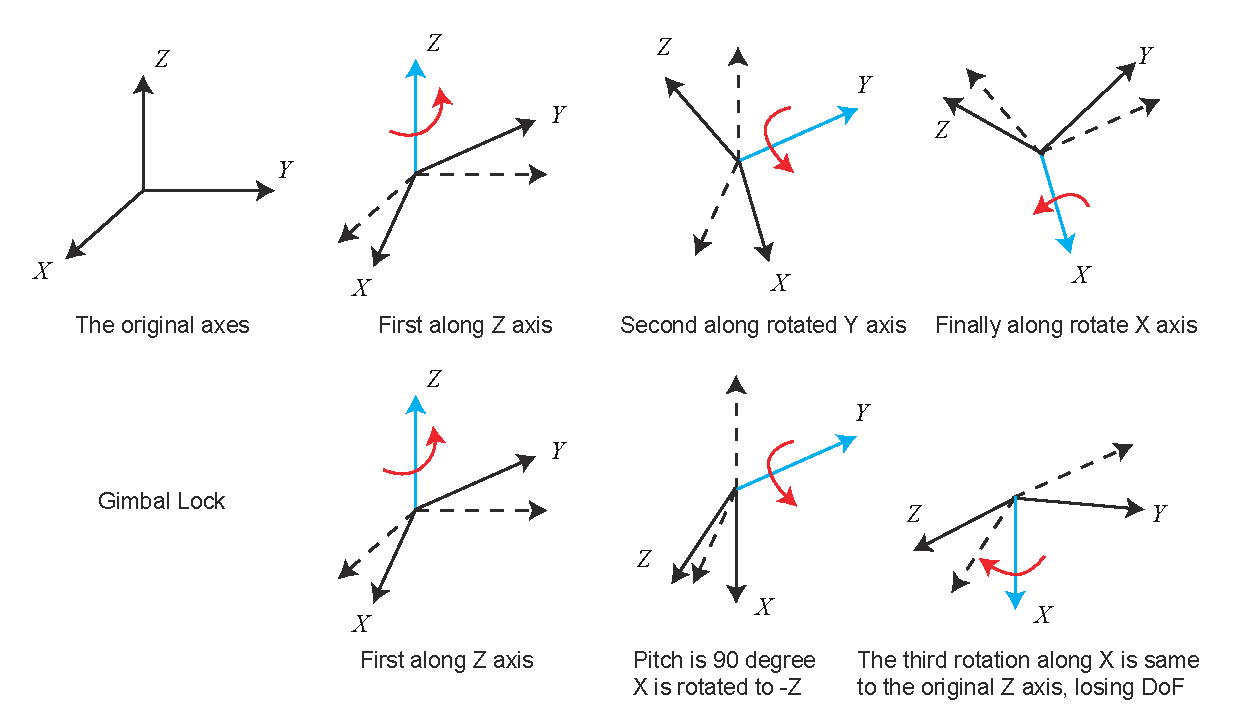
\includegraphics[width=1.0\textwidth]{rigidMotion/eulerAngles.pdf}
	\caption{欧拉角的旋转示意图。上方为ZYX角定义。下方为pitch=$90^\circ$时,第三次旋转与第一次滚转角相同,使得系统丢失了一个自由度。如果你还没有理解万向锁,可以看看相关视频,理解起来会更方便。}
	\label{fig:eulerAngles}
\end{figure}

此时,可以使用$[r,p,y]^\mathrm{T}$这样一个三维的向量描述任意旋转。这个向量十分直观,我们可以从这个向量想象出旋转的过程。其他的欧拉角亦是通过这种方式,把旋转分解到3个轴上,得到一个三维的向量,只不过选用的轴及顺序不一样。这里介绍的rpy角是比较常用的一种,只有很少的欧拉角种类会有rpy这样脍炙人口的名字。不同的欧拉角是按照旋转轴的顺序来称呼的。例如,rpy角的旋转顺序是$ZYX$。同样,也有$XYZ, ZYZ$这样的欧拉角——但是它们就没有专门的名字了。值得一提的是,大部分领域在使用欧拉角时都有各自的坐标方向和顺序上的习惯,不一定和我们这里说的相同。

欧拉角的一个重大缺点是会碰到著名的\textbf{万向锁问题}(Gimbal Lock\footnote{\url{https://en.wikipedia.org/wiki/Gimbal_lock}。}):在俯仰角为$\pm 90 ^\circ $时,第一次旋转与第三次旋转将使用同一个轴,使得系统丢失了一个自由度(由3次旋转变成了2次旋转)。这被称为奇异性问题,在其他形式的欧拉角中也同样存在。理论上可以证明,只要想用3个实数来表达三维旋转时,都会不可避免地碰到奇异性问题\footnote{旋转向量也有奇异性,发生在转角$\theta$超过$2\pi$而产生周期性时。}。由于这种原理,欧拉角不适于插值和迭代,往往只用于人机交互中。我们也很少在SLAM程序中直接使用欧拉角表达姿态,同样不会在滤波或优化中使用欧拉角表达旋转(因为它具有奇异性)。不过,若你想验证自己的算法是否有错,转换成欧拉角能够帮你快速分辨结果是否正确。在某些主体主要为2D运动的场合(例如扫地机、自动驾驶车辆),我们也可以把旋转分解成三个欧拉角,然后把其中一个(例如偏航角)拿出来作为定位信息输出。

\section{四元数}
\subsection{四元数的定义}
旋转矩阵用9个量描述3自由度的旋转,具有冗余性;欧拉角和旋转向量是紧凑的,但具有奇异性。事实上,我们\textbf{找不到不带奇异性的三维向量描述方式}\textsuperscript{\cite{Stuelpnagel1964}}。这有点类似于用两个坐标表示地球表面(如经度和纬度),将必定存在奇异性(纬度为$\pm 90^\circ$时经度无意义)。

回忆以前学习过的复数。我们用复数集$\mathbb{C}$表示复平面上的向量,而复数的乘法则表示复平面上的旋转:例如,乘上复数$i$相当于逆时针把一个复向量旋转$90^\circ$。类似地,在表达三维空间旋转时,也有一种类似于复数的代数:\textbf{四元数}(Quaternion)。四元数是Hamilton找到的一种扩展的复数。它\textbf{既是紧凑的,也没有奇异性}。如果说缺点,四元数不够直观,其运算稍复杂些。

把四元数与复数类比可以帮助你更快地理解四元数。例如,当我们想要将复平面的向量旋转$\theta$角时,可以给这个复向量乘以$\mathrm{e}^{i\theta}$。这是极坐标表示的复数,它也可以写成普通的形式,只要使用欧拉公式即可:
\begin{equation}
\mathrm{e}^{i\theta} = \cos \theta + i \sin \theta.
\end{equation}
这正是一个单位长度的复数。所以,在二维情况下,旋转可以由\textbf{单位复数}来描述。类似地,我们会看到,三维旋转则可以由\textbf{单位四元数}来描述。

一个四元数$\bm{q}$拥有一个实部和三个虚部。本书把实部写在前面(也有地方把实部写在后面),像下面这样:
\begin{equation}
 \bm{q} = q_0 + q_1 i + q_2 j + q_3 k,
\end{equation}
其中$i,j,k$为四元数的三个虚部。这三个虚部满足以下关系式:
\begin{equation}
\label{eq:quaternionVirtual}
\left\{ \begin{array}{l}
{i^2} = {j^2} = {k^2} =  - 1\\
ij = k,ji =  - k\\
jk = i,kj =  - i\\
ki = j,ik =  - j
\end{array} \right. .
\end{equation}
如果把$i,j,k$看成三个坐标轴,那么它们与自己的乘法和复数一样,相互之间的乘法和外积一样。有时人们也用一个标量和一个向量来表达四元数:
\[
 \bm{q} = \left[ s, \bm{v} \right]^\mathrm{T}, \quad s=q_0 \in \mathbb{R},\quad \bm{v} = [q_1, q_2, q_3]^\mathrm{T} \in \mathbb{R}^3,
\]
这里,$s$称为四元数的实部,而$\bm{v}$称为它的虚部。如果一个四元数的虚部为$\bm{0}$,称之为\textbf{实四元数}。反之,若它的实部为$0$,则称之为\textbf{虚四元数}。

%考虑到三维空间需要3个轴,四元数也有3个虚部,那么,一个虚四元数能不能对应到一个空间点呢?事实上我们就是这样做的。

可以用\textbf{单位四元数}表示三维空间中任意一个旋转,不过这种表达方式和复数有着微妙的不同。在复数中,乘以$i$意味着旋转$90^\circ$。这是否意味着四元数中,乘$i$就是绕$i$轴旋转$90^\circ$?那么,$ij=k$是否意味着,先绕$i$转$90^\circ$,再绕$j$转$90^\circ$,就等于绕$k$转$90^\circ$?读者可以找一部手机比划一下——然后你会发现情况并不是这样。正确的情形应该是,乘以$i$对应着旋转$180^\circ$,这样才能保证$ij=k$的性质。而$i^2=-1$,意味着绕$i$轴旋转$360^\circ$后得到一个相反的东西。这个东西要旋转两周才会和它原先的样子相等。

这似乎有些玄妙了,完整的解释需要引入太多额外的东西,我们还是冷静一下回到眼前。至少,我们知道单位四元数能够表达三维空间的旋转。那么四元数本身有些什么性质,它们互相之间又可以做哪些运算呢?下面我们先考察四元数之间的运算法则。

\subsection{四元数的运算}
四元数和通常复数一样,可以进行一系列的运算。常见的有四则运算、数乘、求逆、共轭等。下面分别介绍。

现有两个四元数$\bm{q}_a, \bm{q}_b$,它们的向量表示为$[s_a, \bm{v}_a]^\mathrm{T}, [s_b, \bm{v}_b]^\mathrm{T}$,或者原始四元数表示为:
\[
\bm{q}_a = s_a+x_ai+y_aj+z_ak, \quad \bm{q}_b  = s_b+x_bi+y_bj+z_bk.
\]
那么,其运算可表示如下。

\begin{enumerate}
	\item {\emph{加法和减法}}
	
	四元数$\bm{q}_a, \bm{q}_b$的加减运算为:
	\begin{equation} 	
	\bm{q}_a \pm \bm{q}_b = \left[ s_a \pm s_b, \bm{v}_a \pm \bm{v}_b \right]^\mathrm{T}.
	\end{equation}
	\item{\emph{乘法}}
	
	乘法是把$\bm{q}_a$的每一项与$\bm{q}_b$的每项相乘,最后相加,虚部要按照式\eqref{eq:quaternionVirtual}进行。整理可得:
	\begin{equation}
	\begin{aligned}
	\bm{q}_a \bm{q}_b &= {s_a}{s_b} - {x_a}{x_b} - {y_a}{y_b} - {z_a}{z_b}\\
	&+ \left( {{s_a}{x_b} + {x_a}{s_b} + {y_a}{z_b} - {z_a}{y_b}} \right)i\\
	&+ \left( {{s_a}{y_b} - {x_a}{z_b} + {y_a}{s_b} + {z_a}{x_b}} \right)j\\
	&+ \left( {{s_a}{z_b} + {x_a}{y_b} - {y_a}{x_b} + {z_a}{s_b}} \right)k.
	\end{aligned}
	\end{equation}
	虽然稍为复杂,但形式上是整齐有序的。如果写成向量形式并利用内外积运算,该表达会更加简洁:
	\begin{equation}
	\bm{q}_a \bm{q}_b = \left[ s_a s_b - \bm{v}_a^\mathrm{T} \bm{v}_b, s_a\bm{v}_b + s_b\bm{v}_a + \bm{v}_a \times \bm{v}_b \right]^\mathrm{T}.
	\end{equation}
	在该乘法定义下,两个实的四元数乘积仍是实的,这与复数也是一致的。然而,注意到,由于最后一项外积的存在,四元数乘法通常是不可交换的,除非$\bm{v}_a$和$\bm{v}_b$在$\mathbb{R}^3$中共线,此时外积项为零。

	\item { \emph{模长} }
		
	四元数的模长定义为
	\begin{equation}
	\| \bm{q}_a \| = \sqrt{ s_a^2 + x_a^2 + y_a^2 + z_a^2 }.
	\end{equation}
	可以验证,两个四元数乘积的模即为模的乘积。这使得单位四元数相乘后仍是单位四元数。
	\begin{equation}
	\| \bm{q}_a \bm{q}_b \| = \|\bm{q}_a \| \| \bm{q}_b \|.
	\end{equation}
	
	\item { \emph{共轭} }
	
	四元数的共轭是把虚部取成相反数:
	\begin{equation}
	\bm{q}_a^* = s_a - x_ai - y_aj - z_ak = [s_a, -\bm{v}_a]^\mathrm{T}.
	\end{equation}
	四元数共轭与其本身相乘,会得到一个实四元数,其实部为模长的平方:
	\begin{equation}
	\bm{q}^* \bm{q} = \bm{q} \bm{q}^* = [s_a^2+\bm{v}^\mathrm{T} \bm{v}, \bm{0} ]^\mathrm{T}.
	\end{equation}

	\item{ \emph{逆} }
	
	一个四元数的逆为
	\begin{equation}
	\label{eq:quaternionInverse}
	\bm{q}^{-1} = \bm{q}^* / \| \bm{q} \| ^2.
	\end{equation}
	按此定义,四元数和自己的逆的乘积为实四元数$\bm{1}$:
	\begin{equation}
	\bm{q} \bm{q}^{-1} = \bm{q}^{-1} \bm{q} = \bm{1}.
	\end{equation}
	
	如果$\bm{q}$为单位四元数,其逆和共轭就是同一个量。同时,乘积的逆有和矩阵相似的性质:
	\begin{equation}
	\left( \bm{q}_a \bm{q}_b \right)^{-1} = \bm{q}_b^{-1} \bm{q}_a^{-1}.
	\end{equation}
	
	\item{ \emph{数乘} }
	
	和向量相似,四元数可以与数相乘:
	\begin{equation}
	k \bm{q} = \left[ ks, k\bm{v} \right]^\mathrm{T}.
	\end{equation}
\end{enumerate}

\subsection{用四元数表示旋转}
我们可以用四元数表达对一个点的旋转。假设一个空间三维点$\bm{p} = [x,y,z]\in \mathbb{R}^3$,以及一个由单位四元数$\bm{q}$指定的旋转。三维点$\bm{p}$经过旋转之后变为$\bm{p}'$。如果使用矩阵描述,那么有$\bm{p}'=\bm{R} \bm{p}$。而如果用四元数描述旋转,它们的关系又如何来表达呢?

首先,把三维空间点用一个虚四元数来描述:
\[
\bm{p} = [0, x, y, z]^\mathrm{T} = [0, \bm{v}]^\mathrm{T}. 
\]
相当于把四元数的3个虚部与空间中的3个轴相对应。那么,旋转后的点$\bm{p}'$即可表示为这样的乘积:
\begin{equation}\label{eq:rotate-with-quaternion}
\bm{p}' = \bm{q} \bm{p} \bm{q}^{-1}.
\end{equation}
这里的乘法均为四元数乘法,结果也是四元数。最后把$\bm{p}'$的虚部取出,即得旋转之后点的坐标。并且,可以验证(留作习题),计算结果的实部为0,故为纯虚四元数。

\subsection{四元数到其他旋转表示的转换}
任意单位四元数描述了一个旋转,该旋转亦可用旋转矩阵或旋转向量描述。现在来考察四元数与旋转向量、旋转矩阵之间的转换关系。在此之前,我们要说,四元数乘法也可以写成一种矩阵的乘法。设$\bm{q}=[s,\bm{v}]^\mathrm{T}$,那么,定义如下的符号$^{+}$和$^{\oplus}$为\textsuperscript{\cite{Barfoot2011}}:
\begin{equation}
\bm{q}^{+}=\left[\begin{array}{cc}
s&-\bm{v}^\mathrm{T} \\
\bm{v}&s\bm{I}+\bm{v}^{\wedge}
\end{array}\right],\quad 
\bm{q}^{\oplus}=
\left[\begin{array}{cc}
s & -\bm{v}^\mathrm{T} \\
\bm{v} & s\bm{I}-\bm{v}^{\wedge}
\end{array}\right],
\end{equation}
这两个符号将四元数映射成为一个4$\times$4的矩阵。于是四元数乘法可以写成矩阵的形式:
\begin{equation}
\bm{q}_1^ + {\bm{q}_2} = \left[ {\begin{array}{*{20}{c}}
	s_1&-\bm{v}_1^T\\
	\bm{v}_1 & s_1 \bm{I} + \bm{v}_1^\wedge
	\end{array}} \right]\left[ {\begin{array}{*{20}{c}}
	{{s _2}} \\
	{{\bm{v} _2}}
	\end{array}} \right] = \left[ {\begin{array}{*{20}{c}}
	{ - \bm{v} _1^T{\bm{v} _2} + {s _1}{s _2}} \\ 
	{{s _1}{\bm{v} _2} + {s _2}{\bm{v} _1} + \bm{v} _1^ \wedge {\bm{v} _2}}
	\end{array}} \right] = \bm{q}_1 \bm{q}_2
\end{equation}
同理亦可证:
\begin{equation}
\bm{q}_1 \bm{q}_2 = \bm{q}_1^{+} \bm{q}_2 = \bm{q}_2^{\oplus} \bm{q}_1.
\end{equation}

然后,考虑使用四元数对空间点进行旋转的问题。根据前面的说法,有:
\begin{equation}
\begin{split}
\bm{p}' &= \bm{q} \bm{p} \bm{q}^{-1} = \bm{q}^+ \bm{p}^+ \bm{q}^{-1} \\
&= \bm{q}^+ \bm{q}^{{-1}^{\oplus}} \bm{p}.
\end{split}
\end{equation}
代入两个符号对应的矩阵,得:
\begin{equation}\label{eq:quaternion-to-rotation-matrix-derive}
{\bm{q}^ + }{\left( {{\bm{q}^{ - 1}}} \right)^ \oplus } = \left[ \begin{array}{*{20}{c}}
	s&-\bm{v}^T\\
	\bm{v}&s\bm{I}+\bm{v}^\wedge 
	\end{array} \right]\left[\begin{array}{*{20}{c}}
	s&{\bm{v} ^T}\\
	{ - \bm{v} }&{s\bm{I} + \bm{v} ^ \wedge }
	\end{array} \right] = \left[ \begin{array}{*{20}{c}}
	1&\bm{0} \\
	\bm{0}^\mathrm{T}&\bm{v}\bm{v}^\mathrm{T} + {s^2} \bm{I} + 2s\bm{v} ^ \wedge + {(\bm{v} ^ \wedge)}^2 
	\end{array} \right].
\end{equation}
因为$\bm{p}'$和$\bm{p}$都是虚四元数,那么事实上该矩阵的右下角即给出了\textbf{从四元数到旋转矩阵}的变换关系:
\begin{equation}
\bm{R} = \bm{v} \bm{v}^\mathrm{T} + {s^2} \bm{I} + 2s\bm{v} ^ \wedge + {(\bm{v} ^ \wedge)}^2.
\end{equation}
为了得到四元数到旋转向量的转换公式,对上式两侧求迹,得:
\begin{equation}
\begin{aligned}
\mathrm{tr}(\bm{R}) &= \mathrm{tr}(\bm{v}\bm{v}^\mathrm{T} + 3s^2 + 2s \cdot 0 + \mathrm{tr}((\bm{v}^\wedge)^2) \\
&= v_1^2+v_2^2+v_3s^2 + 3s^2 - 2(v_1^2+v_2^2+v_3^2) \\
&= (1-s^2) + 3s^2 -2(1-s^2)\\
&= 4s^2 -1.
\end{aligned}
\end{equation}
又由式\eqref{eq:R2theta}得:
\begin{equation}
\begin{aligned}
\theta &= \arccos(\frac{\mathrm{tr}(\bm{R}-1)}{2}) \\
&=\arccos(2s^2-1).
\end{aligned}
\end{equation}
即
\begin{equation}
\cos \theta =2s^2-1=2 \cos^2 \frac{\theta}{2} -1,
\end{equation}
所以:
\begin{equation}
\theta = 2 \arccos s.
\end{equation}
至于旋转轴,如果在式\eqref{eq:quaternion-to-rotation-matrix-derive}中用$\bm{q}$的虚部代替$\bm{p}$,易知$\bm{q}$的虚部组成的向量在旋转时是不动的,即构成旋转轴。于是只要将它除掉它的模长,即得。总而言之,四元数到旋转向量的转换公式可列写如下:
\begin{equation}
\label{eq:rotationVector2Quaternion}
\begin{cases}
\theta  = 2\arccos {q_0}\\
{\left[ {{n_x},{n_y},{n_z}} \right]^\mathrm{T}} = {{{\left[ {{q_1},{q_2},{q_3}} \right]}^\mathrm{T}}}/{\sin \frac{\theta }{2}}
\end{cases} .
\end{equation}

至于如何从其他方式转换到四元数,只须把上述步骤倒过来处理即可。在实际编程中,程序库通常会为我们准备好各种形式之间的转换。无论是四元数、旋转矩阵还是轴角,它们都可以用来描述同一个旋转。我们应该在实际中选择最为方便的形式,而不必拘泥于某种特定的形式。在随后的实践和习题中,我们会演示各种表达方式之间的转换,以加深读者的印象。


%
%从旋转向量到四元数的转换方式已在式\eqref{eq:rotationVector2Quaternion}中给出。因此,现在看来把四元数转换为矩阵的最直观方法,是先把四元数$\bm{q}$转换为轴角$\theta$和$\bm{n}$,然后再根据罗德里格斯公式转换为矩阵。不过那样要计算一个$\arccos$函数,代价较大。实际上这个计算是可以通过一定的技巧绕过的。这里省略推导过程,直接给出四元数到旋转矩阵的转换方式。
%
%这种表达方式和旋转矩阵、旋转向量有什么关系呢?我们不妨先来看旋转向量。假设某个旋转是绕单位向量$\bm{n}=\left[ n_x, n_y, n_z \right]^\mathrm{T}$进行了角度为$\theta$的旋转,那么这个旋转的四元数形式为
%\begin{equation}
%\label{eq:ntheta2quaternion}
%\bm{q} = \left[ \cos \frac{\theta}{2}, n_x \sin \frac{\theta}{2}, n_y \sin \frac{\theta}{2}, n_z \sin \frac{\theta}{2}\right]^\mathrm{T} .
%\end{equation}
%
%反之,亦可从单位四元数中计算出对应旋转轴与夹角:
%
%
%这个式子给了我们一种微妙的“转了一半”的感觉。同样,对式\eqref{eq:ntheta2quaternion}的$\theta$加上$2\pi$,我们得到一个相同的旋转,但此时对应的四元数变成了$-\bm{q}$。因此,在四元数中,\textbf{任意的旋转都可以由两个互为相反数的四元数表示}。同理,取$\theta$为$0$,则得到一个没有任何旋转的实四元数:
%\begin{equation}
%\bm{q}_0 = \left[ { \pm 1,0,0,0} \right]^\mathrm{T} .
%\end{equation}
%
%设四元数$\bm{q} = q_0+q_1i+q_2j+q_3k$,对应的旋转矩阵$\bm{R}$为
%\begin{equation}
%\bm{R} = \left[ {\begin{array}{*{20}{c}}
%	 {1 - 2q_2^2 - 2q_3^2}&{2{q_1}{q_2} - 2{q_0}{q_3}}&{2{q_1}{q_3} + 2{q_0}{q_2}}\\
%	 {2{q_1}{q_2} + 2{q_0}{q_3}}&{1 - 2q_1^2 - 2q_3^2}&{2{q_2}{q_3} - 2{q_0}{q_1}}\\
%	 {2{q_1}{q_3} - 2{q_0}{q_2}}&{2{q_2}{q_3} + 2{q_0}{q_1}}&{1 - 2q_1^2 - 2q_2^2}
% \end{array}} \right].
%\end{equation}
%
%反之,由旋转矩阵到四元数的转换如下。假设矩阵为$\bm{R}=\{ m_{ij}\}, i, j \in \left[ 1, 2,3 \right] $,其对应的四元数$\bm{q}$由下式给出:
%\begin{equation}
%{q_0} = \frac{{\sqrt {\mathrm{tr}(R) + 1} }}{2},{q_1} = \frac{{{m_{23}} - {m_{32}}}}{{4{q_0}}},{q_2} = \frac{{{m_{31}} - {m_{13}}}}{{4{q_0}}},{q_3} = \frac{{{m_{12}} - {m_{21}}}}{{4{q_0}}}.
%\end{equation}
%
%值得一提的是,由于$\bm{q}$和$\bm{-q}$表示同一个旋转,事实上一个$\bm{R}$对应的四元数表示并不是唯一的。同时,除了上面给出的转换方式之外,还存在其他几种计算方法,而本书都省略了。实际编程中,当$q_0$接近0时,其余3个分量会非常大,导致解不稳定,此时我们再考虑使用其他的方式进行转换。

\section{\textsuperscript{\ttfamily *}相似、仿射、射影变换}
除了欧氏变换之外,3D空间还存在其他几种变换方式,只不过欧氏变换是最简单的。它们一部分和测量几何有关,因为在之后的讲解中可能会提到,所以先罗列出来。欧氏变换保持了向量的长度和夹角,相当于我们把一个刚体原封不动地进行了移动或旋转,不改变它自身的样子。其他几种变换则会改变它的外形。它们都拥有类似的矩阵表示。

\begin{enumerate}
	\item {\emph{相似变换}}
	
	相似变换比欧氏变换多了一个自由度,它允许物体进行均匀缩放,其矩阵表示为
	\begin{equation}
	\bm{T}_S = \left[ {\begin{array}{*{20}{c}}
		{s \bm{R}}& \bm{t}\\
		{{ \bm{0}^\mathrm{T}}}&1
		\end{array}} \right].
	\end{equation}
	
	注意到旋转部分多了一个缩放因子$s$,表示我们在对向量旋转之后,可以在$x,y,z$三个坐标上进行均匀缩放。由于含有缩放,相似变换不再保持图形的面积不变。你可以想象一个边长为1的立方体通过相似变换后,变成边长为10的样子(但仍然是立方体)。三维相似变换的集合也叫做\textbf{相似变换群},记作$\mathrm{Sim}(3)$。
	
	\item { \emph{仿射变换} }
	
	仿射变换的矩阵形式如下:
	\begin{equation}
	\bm{T}_A = \left[ {\begin{array}{*{20}{c}}
		\bm{A} & \bm{t}\\
		{{\bm{0}^\mathrm{T}}} & 1
		\end{array}} \right].
	\end{equation}
	
	与欧氏变换不同的是,仿射变换只要求$\bm{A}$是一个可逆矩阵,而不必是正交矩阵。仿射变换也叫正交投影。经过仿射变换之后,立方体就不再是方的了,但是各个面仍然是平行四边形。
	
	\item{ \emph{射影变换} }
	
	射影变换是最一般的变换,它的矩阵形式为
	
	\begin{equation}
	{\bm{T}_P} = \left[ {\begin{array}{*{20}{c}}
		\bm{A} & \bm{t}\\
		{{\bm{a}^\mathrm{T}}} & v
		\end{array}} \right].
	\end{equation}
	
	它的左上角为可逆矩阵$\bm{A}$,右上角为平移$\bm{t}$,左下角为缩放$\bm{a}^\mathrm{T}$。由于采用了齐次坐标,当$v \neq 0$时,我们可以对整个矩阵除以$v$得到一个右下角为1的矩阵; 否则得到右下角为$0$的矩阵。因此,2D的射影变换一共有8个自由度,3D则共有15个自由度。射影变换是现在讲过的变换中,形式最为一般的。从真实世界到相机照片的变换可以看成一个射影变换。读者可以想象一个原本方形的地板砖,在照片当中是什么样子:首先,它不再是方形的。由于近大远小的关系,它甚至不是平行四边形,而是一个不规则的四边形。
\end{enumerate}

\autoref{table:common-transform}总结了目前讲到的几种变换的性质。注意在“不变性质”中,从上到下是有包含关系的。例如,欧氏变换除了保体积之外,也具有保平行、相交等性质。

\begin{table}[!htp]
	\centering
	\caption{常见变换性质比较}
	\label{table:common-transform}
	\begin{tabu}{c|c|c|c}
		\toprule
		变换名称 & 矩阵形式 & 自由度 & 不变性质 \\ \midrule
		欧氏变换 \rule{0pt}{20 pt} & $\left[ {\begin{array}{*{20}{c}}
			\bm{R} & \bm{t}\\
			{{\bm{0}^\mathrm{T}}}&1
			\end{array}} \right]$ & 6 & 长度、夹角、体积 \\ 
		相似变换 \rule{0pt}{20 pt}& $ \left[ {\begin{array}{*{20}{c}}
			{s \bm{R}}& \bm{t}\\
			{{ \bm{0}^\mathrm{T}}}&1
			\end{array}} \right]$ & 7 & 体积比 \\ 
		仿射变换 \rule{0pt}{20 pt}& $ \left[ {\begin{array}{*{20}{c}}
			\bm{A} & \bm{t}\\
			{{\bm{0}^\mathrm{T}}} & 1
			\end{array}} \right]$   & 12 & 平行性、体积比 \\ 
		射影变换 \rule{0pt}{20 pt} & $ \left[ {\begin{array}{*{20}{c}}
			\bm{A} & \bm{t}\\
			{{\bm{a}^\mathrm{T}}} & v
			\end{array}} \right]$ & 15 & 接触平面的相交和相切 \rule{0pt}{20 pt}\\ 
		\bottomrule
	\end{tabu} 
\end{table}

我们之后会说到,从真实世界到相机照片的变换是一个射影变换。如果相机的焦距为无穷远,那么这个变换为仿射变换。不过,在详细讲述相机模型之前,我们只要对它们有个大致的印象即可。

\section{实践:Eigen几何模块}
\subsection{Eigen几何模块的数据演示}
现在,我们来实际演练一下前面讲到的各种旋转表达方式。我们将在Eigen中使用四元数、欧拉角和旋转矩阵,演示它们之间的变换方式。我们还会给出一个可视化程序,帮助读者理解这几个变换的关系。

\begin{lstlisting}[language=c++,caption=slambook2/ch3/useGeometry/useGeometry.cpp]
#include <iostream>
#include <cmath>
using namespace std;

#include <Eigen/Core>
#include <Eigen/Geometry>

using namespace Eigen;
// 本程序演示了 Eigen 几何模块的使用方法

int main(int argc, char **argv) {
    // Eigen/Geometry 模块提供了各种旋转和平移的表示
    // 3D 旋转矩阵直接使用 Matrix3d 或 Matrix3f
    Matrix3d rotation_matrix = Matrix3d::Identity();
    // 旋转向量使用 AngleAxis, 它底层不直接是Matrix,但运算可以当作矩阵(因为重载了运算符)
    AngleAxisd rotation_vector(M_PI / 4, Vector3d(0, 0, 1));     //沿 Z 轴旋转 45 度
    cout.precision(3);
    cout << "rotation matrix =\n" << rotation_vector.matrix() << endl;   //用matrix()转换成矩阵
    // 也可以直接赋值
    rotation_matrix = rotation_vector.toRotationMatrix();
    // 用 AngleAxis 可以进行坐标变换
    Vector3d v(1, 0, 0);
    Vector3d v_rotated = rotation_vector * v;
    cout << "(1,0,0) after rotation (by angle axis) = " << v_rotated.transpose() << endl;
    // 或者用旋转矩阵
    v_rotated = rotation_matrix * v;
    cout << "(1,0,0) after rotation (by matrix) = " << v_rotated.transpose() << endl;
    
    // 欧拉角: 可以将旋转矩阵直接转换成欧拉角
    Vector3d euler_angles = rotation_matrix.eulerAngles(2, 1, 0); // ZYX顺序,即roll pitch yaw顺序
    cout << "yaw pitch roll = " << euler_angles.transpose() << endl;
    
    // 欧氏变换矩阵使用 Eigen::Isometry
    Isometry3d T = Isometry3d::Identity();       // 虽然称为3d,实质上是4*4的矩阵
    T.rotate(rotation_vector);                   // 按照rotation_vector进行旋转
    T.pretranslate(Vector3d(1, 3, 4));           // 把平移向量设成(1,3,4)
    cout << "Transform matrix = \n" << T.matrix() << endl;
    
    // 用变换矩阵进行坐标变换
    Vector3d v_transformed = T * v;                              // 相当于R*v+t
    cout << "v tranformed = " << v_transformed.transpose() << endl;
    
    // 对于仿射和射影变换,使用 Eigen::Affine3d 和 Eigen::Projective3d 即可,略
    
    // 四元数
    // 可以直接把AngleAxis赋值给四元数,反之亦然
    Quaterniond q = Quaterniond(rotation_vector);
    cout << "quaternion from rotation vector = " << q.coeffs().transpose()
    << endl;   // 请注意coeffs的顺序是(x,y,z,w),w为实部,前三者为虚部
    // 也可以把旋转矩阵赋给它
    q = Quaterniond(rotation_matrix);
    cout << "quaternion from rotation matrix = " << q.coeffs().transpose() << endl;
    // 使用四元数旋转一个向量,使用重载的乘法即可
    v_rotated = q * v; // 注意数学上是qvq^{-1}
    cout << "(1,0,0) after rotation = " << v_rotated.transpose() << endl;
    // 用常规向量乘法表示,则应该如下计算
    cout << "should be equal to " << (q * Quaterniond(0, 1, 0, 0) * q.inverse()).coeffs().transpose() << endl;
    
    return 0;
}
\end{lstlisting}

Eigen中对各种形式的表达方式总结如下。请注意每种类型都有单精度和双精度两种数据类型,而且和之前一样,不能由编译器自动转换。下面以双精度为例,你可以把最后的d改成f,即得到单精度的数据结构。
\begin{itemize}
	\item 旋转矩阵($3 \times 3$):Eigen::Matrix3d。
	\item 旋转向量($3 \times 1$):Eigen::AngleAxisd。
	\item 欧拉角($3 \times 1$):Eigen::Vector3d。
	\item 四元数($4 \times 1$):Eigen::Quaterniond。
	\item 欧氏变换矩阵($4 \times 4$):Eigen::Isometry3d。
	\item 仿射变换($4 \times 4$):Eigen::Affine3d。
	\item 射影变换($4 \times 4$):Eigen::Projective3d。
\end{itemize}

参考代码中对应的CMakeLists即可编译此程序。在这个程序中,演示了如何使用Eigen中的旋转矩阵、旋转向量(AngleAxis)、欧拉角和四元数。我们用这几种旋转方式去旋转一个向量$\bm{v}$,发现结果是一样的(不一样就真是见鬼了)。同时,也演示了如何在程序中转换这几种表达方式。想进一步了解Eigen的几何模块的读者可以参考(\url{http://eigen.tuxfamily.org/dox/group__TutorialGeometry.html})。

请读者注意,\textbf{程序代码通过和数学表示有一些细微的差别}。例如,通过运算符重载,四元数和三维向量可以直接计算乘法,但在数学上则需要先把向量转成虚四元数,再利用四元数乘法进行计算,同样的情况也适用于变换矩阵乘三维向量的情况。总体而言,程序中的用法会比数学公式更灵活一些。

\subsection{实际的坐标变换例子}
下面我们举一个小例子来演示坐标变换。

\noindent \textbf{例子} \quad \emph{设有小萝卜一号和小萝卜二号位于世界坐标系中。记世界坐标系为$W$,小萝卜们的坐标系为$R_1$和$R_2$。小萝卜一号的位姿为$\bm{q}_1 = [ 0.35, 0.2, 0.3, 0.1 ]^\mathrm{T}, \bm{t}_1 = [0.3, 0.1, 0.1]^\mathrm{T}$。小萝卜二号的位姿为$\bm{q}_2 = [ -0.5, 0.4, -0.1, 0.2 ]^\mathrm{T}, \bm{t}_2 = [-0.1, 0.5, 0.3]^\mathrm{T}$。这里的$\bm{q}$和$\bm{t}$表达的是$\bm{T}_{R_k, W},k=1,2$,也就是世界坐标系到相机坐标系的变换关系。现在,小萝卜一号看到某个点在自身的坐标系下坐标为$\bm{p}_{R_1} = [0.5,0,0.2]^\mathrm{T}$,求该向量在小萝卜二号坐标系下的坐标。}

这是一个非常简单,但又具有代表性的例子。在实际场景中你经常需要在同一个机器人的不同部分,或者不同机器人之间转换坐标。下面我们书写一段程序来演示这个计算。

\begin{lstlisting}[language=c++,caption=slambook2/ch3/examples/coordinateTransform.cpp]
#include <iostream>
#include <vector>
#include <algorithm>
#include <Eigen/Core>
#include <Eigen/Geometry>

using namespace std;
using namespace Eigen;

int main(int argc, char** argv) {
    Quaterniond q1(0.35, 0.2, 0.3, 0.1), q2(-0.5, 0.4, -0.1, 0.2);
    q1.normalize();
    q2.normalize();
    Vector3d t1(0.3, 0.1, 0.1), t2(-0.1, 0.5, 0.3);
    Vector3d p1(0.5, 0, 0.2);
    
    Isometry3d T1w(q1), T2w(q2);
    T1w.pretranslate(t1);
    T2w.pretranslate(t2);
    
    Vector3d p2 = T2w * T1w.inverse() * p1;
    cout << endl << p2.transpose() << endl;
    return 0;
}
\end{lstlisting}

程序输出的答案是$[-0.0309731,0.73499,0.296108]^\mathrm{T}$,计算过程也十分简单,只需计算$$\bm{p}_{R_2} = \bm{T}_{R_2,W}\bm{T}_{W, R_1} \bm{p}_{R_1}$$即可。注意四元数使用之前需要归一化。

\section{可视化演示}
\subsection{显示运动轨迹}
如果你是第一次接触旋转和平移这些概念,可能会觉得它们形式看起来很复杂,因为毕竟每种表达方式都可以与其他方式互相转换,而转换公式有时还比较长。不过,虽然旋转矩阵、变换矩阵的数值可能不够直观,但我们可以很容易地把它们画在窗口里面。

本节我们演示两个可视化例子。首先,假设我们通过某种方式记录了一个机器人的运动轨迹,现在想把它画到一个窗口中。假设轨迹文件存储于trajectory.txt,每一行用下面的格式存储:$$\mathrm{time}, t_x, t_y, t_z, q_x, q_y, q_z, q_w,$$其中$\mathrm{time}$指该位姿的记录时间,$\bm{t}$为平移,$\bm{q}$为旋转四元数,均是以世界坐标系到机器人坐标系记录。下面我们从文件中读取这些轨迹,并显示到一个窗口中。原则上,如果只是谈论“机器人的位姿”,那么你可以使用$\bm{T}_{WR}$或者$\bm{T}_{RW}$,事实上它们也只差一个逆而已,意味着知道其中一个就可以很轻松地得到另一个。如果你想要存储\textbf{机器人的轨迹},那么你可以存储所有时刻的$\bm{T}_{WR}$或者$\bm{T}_{RW}$,这并没有太大的差别。

在画轨迹的时候,我们可以把“轨迹”画成一系列点组成的序列,这和我们想象中的“轨迹”比较相似。严格说来,这其实是\textbf{机器人(相机)坐标系的原点在世界坐标系中的坐标}。考虑机器人坐标系的原点,即$\bm{O}_{R}$,那么,此时的$\bm{O}_{W}$就是这个原点在世界坐标系下的坐标:
\begin{equation}
\bm{O}_{W} = \bm{T}_{WR} \bm{O}_R = \bm{t}_{WR}.
\end{equation}
这正是$\bm{T}_{WR}$的平移部分。因此,可以从$\bm{T}_{WR}$中直接看到\textbf{相机在何处},这也是我们说$\bm{T}_{WR}$更为直观的原因。因此,在可视化程序里,轨迹文件存储了$\bm{T}_{WR}$而不是$\bm{T}_{RW}$。

最后,我们需要一个支持3D绘图的程序库。有许多库都支持3D绘图,比如大家熟悉的matlab,python的matplotlib,OpenGL等。在linux中,一个常见的库是基于OpenGL的Pangolin库\footnote{\url{https://github.com/stevenlovegrove/Pangolin}},它在支持OpenGL的绘图操作基础之上还提供了一些GUI的功能。在第二版的书籍中,我们使用git的submodule功能来管理本书依赖的第三方库。读者可以进入3rdparty文件夹中直接安装所需的库,git保证了我和你使用的版本是一致的。

\begin{lstlisting}[language=c++,caption=slambook2/ch3/examples/plotTrajectory.cpp]
#include <pangolin/pangolin.h>
#include <Eigen/Core>
#include <unistd.h>

using namespace std;
using namespace Eigen;

// path to trajectory file
string trajectory_file = "./examples/trajectory.txt";

void DrawTrajectory(vector<Isometry3d, Eigen::aligned_allocator<Isometry3d>>);

int main(int argc, char **argv) {
    vector<Isometry3d, Eigen::aligned_allocator<Isometry3d>> poses;
    ifstream fin(trajectory_file);
    if (!fin) {
        cout << "cannot find trajectory file at " << trajectory_file << endl;
        return 1;
    }
    
    while (!fin.eof()) {
        double time, tx, ty, tz, qx, qy, qz, qw;
        fin >> time >> tx >> ty >> tz >> qx >> qy >> qz >> qw;
        Isometry3d Twr(Quaterniond(qw, qx, qy, qz));
        Twr.pretranslate(Vector3d(tx, ty, tz));
        poses.push_back(Twr);
    }
    cout << "read total " << poses.size() << " pose entries" << endl;
    
    // draw trajectory in pangolin
    DrawTrajectory(poses);
    return 0;
}

void DrawTrajectory(vector<Isometry3d, Eigen::aligned_allocator<Isometry3d>> poses) {
    // create pangolin window and plot the trajectory
    pangolin::CreateWindowAndBind("Trajectory Viewer", 1024, 768);
    glEnable(GL_DEPTH_TEST);
    glEnable(GL_BLEND);
    glBlendFunc(GL_SRC_ALPHA, GL_ONE_MINUS_SRC_ALPHA);
    
    pangolin::OpenGlRenderState s_cam(
    pangolin::ProjectionMatrix(1024, 768, 500, 500, 512, 389, 0.1, 1000),
    pangolin::ModelViewLookAt(0, -0.1, -1.8, 0, 0, 0, 0.0, -1.0, 0.0)
    );
    
    pangolin::View &d_cam = pangolin::CreateDisplay()
        .SetBounds(0.0, 1.0, 0.0, 1.0, -1024.0f / 768.0f)
        .SetHandler(new pangolin::Handler3D(s_cam));
    
    while (pangolin::ShouldQuit() == false) {
        glClear(GL_COLOR_BUFFER_BIT | GL_DEPTH_BUFFER_BIT);
        d_cam.Activate(s_cam);
        glClearColor(1.0f, 1.0f, 1.0f, 1.0f);
        glLineWidth(2);
        for (size_t i = 0; i < poses.size(); i++) {
            // 画每个位姿的三个坐标轴
            Vector3d Ow = poses[i].translation();
            Vector3d Xw = poses[i] * (0.1 * Vector3d(1, 0, 0));
            Vector3d Yw = poses[i] * (0.1 * Vector3d(0, 1, 0));
            Vector3d Zw = poses[i] * (0.1 * Vector3d(0, 0, 1));
            glBegin(GL_LINES);
            glColor3f(1.0, 0.0, 0.0);
            glVertex3d(Ow[0], Ow[1], Ow[2]);
            glVertex3d(Xw[0], Xw[1], Xw[2]);
            glColor3f(0.0, 1.0, 0.0);
            glVertex3d(Ow[0], Ow[1], Ow[2]);
            glVertex3d(Yw[0], Yw[1], Yw[2]);
            glColor3f(0.0, 0.0, 1.0);
            glVertex3d(Ow[0], Ow[1], Ow[2]);
            glVertex3d(Zw[0], Zw[1], Zw[2]);
            glEnd();
        }
        // 画出连线
        for (size_t i = 0; i < poses.size(); i++) {
            glColor3f(0.0, 0.0, 0.0);
            glBegin(GL_LINES);
            auto p1 = poses[i], p2 = poses[i + 1];
            glVertex3d(p1.translation()[0], p1.translation()[1], p1.translation()[2]);
            glVertex3d(p2.translation()[0], p2.translation()[1], p2.translation()[2]);
            glEnd();
        }
        pangolin::FinishFrame();
        usleep(5000);   // sleep 5 ms
    }
}
\end{lstlisting}

该程序演示了如何在Pangolin中画出3D的位姿。我们用红、绿、蓝三种颜色画出每个位姿的三个坐标轴(实际上我们计算了各坐标轴的世界坐标),然后用黑色线将轨迹连起来。程序运行结果如\autoref{fig:trajectory}所示。

\begin{figure}[!htp]
    \centering
    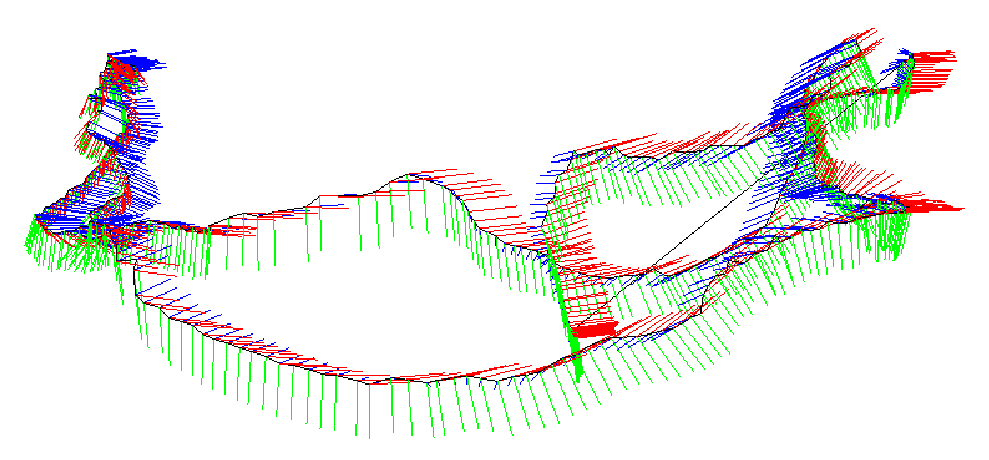
\includegraphics[width=0.8\textwidth]{rigidMotion/trajectory.pdf}
    \caption{位姿可视化的结果}
    \label{fig:trajectory}
\end{figure}

\subsection{显示相机的位姿}
\begin{figure}[!htp]
    \centering
    \includegraphics[width=0.8\textwidth]{rigidMotion/visualizeGeometry.pdf}
    \caption{旋转矩阵、欧拉角、四元数的可视化程序。}
    \label{fig:visualizeGeometry}
\end{figure}
除了显示轨迹之外,我们也可以显示3D窗口中相机的位姿。在slambook2/ch3/visualizeGeometry中,我们以可视化的形式演示了相机位姿的各种表达方式(见\autoref{fig:visualizeGeometry})。当读者用鼠标操作相机时,左侧的方框里会实时显示相机位姿对应的旋转矩阵、平移、欧拉角和四元数,你可以看看数据是如何变化的。根据我们的经验,除了欧拉角之外,你应该看不出它们直观的含义。然而,尽管旋转矩阵或变换矩阵并不直观,但是将它们可视化地显示出来并没有什么困难。该程序使用Pangolin库作为3D显示库,请参考Readme.txt来编译该程序。

\section*{习题}
\begin{enumerate}
	\item 验证旋转矩阵是正交矩阵。
	\item[\optional] 寻找罗德里格斯公式的推导过程并加以理解。
	\item 验证四元数旋转某个点后,结果是一个虚四元数(实部为零),所以仍然对应到一个三维空间点,见式\eqref{eq:rotate-with-quaternion}。
	\item 画表总结旋转矩阵、轴角、欧拉角、四元数的转换关系。
	\item 假设有一个大的Eigen矩阵,想把它的左上角$3 \times 3$的块取出来,然后赋值为$\bm{I}_{3 \times 3}$。请编程实现。
	\item[\optional] 一般线性方程$\bm{A} \bm{x}=\bm{b}$有哪几种做法?你能在Eigen中实现吗?
\end{enumerate}
% ch4 李代数
% !Mode:: "TeX:UTF-8"
\chapter{李群与李代数}
\label{cpt:4}
\begin{mdframed}  
	\textbf{主要目标}
	\begin{enumerate}[labelindent=0em,leftmargin=1.5em]
		\item 理解李群与李代数的概念,掌握$\mathrm{SO}(3), \mathrm{SE}(3)$与对应李代数的表示方式。
		\item 理解BCH近似的意义。
		\item 学会在李代数上的扰动模型。
		\item 使用Sophus对李代数进行运算。
	\end{enumerate}
\end{mdframed} 

上一讲,我们介绍了三维世界中刚体运动的描述方式,包括旋转矩阵、旋转向量、欧拉角、四元数等若干种方式。我们重点介绍了旋转的表示,但是在SLAM中,除了表示之外,我们还要对它们进行估计和优化。因为在SLAM中位姿是未知的,而我们需要解决形如“\textbf{什么样的相机位姿最符合当前观测数据}”这样的问题。一种典型的方式是把它构建成一个优化问题,求解最优的$\bm{R}, \bm{t}$,使得误差最小化。

如前所言,旋转矩阵自身是带有约束的(正交且行列式为1)。它们作为优化变量时,会引入额外的约束,使优化变得困难。通过李群—李代数间的转换关系,我们希望把位姿估计变成无约束的优化问题,简化求解方式。考虑到读者可能还没有李群李代数的基本知识,我们将从最基本的知识开始讲起。
\newpage
\includepdf{resources/other/ch4.pdf}

\newpage 
\section{李群与李代数基础}
上一讲,我们介绍了旋转矩阵和变换矩阵的定义。当时,我们说三维旋转矩阵构成了\textbf{特殊正交群}$\mathrm{SO}(3)$,而变换矩阵构成了\textbf{特殊欧氏群}$\mathrm{SE}(3)$。它们写起来像这样:
\begin{equation}
\mathrm{SO}(3) = \{ \bm{R} \in \mathbb{R}^{3 \times 3} | \bm{R R}^\mathrm{T} = \bm{I}, \det(\bm{R})=1 \}.
\end{equation}
\begin{equation}
\mathrm{SE}(3) = \left\{ \bm{T} = \left[ {\begin{array}{*{20}{c}}
	\bm{R} & \bm{t} \\
	{{\bm{0}^\mathrm{T}}} & 1
	\end{array}} \right]
\in \mathbb{R}^{4 \times 4} | \bm{R} \in \mathrm{SO}(3), \bm{t} \in \mathbb{R}^3\right\}.
\end{equation}

不过,当时我们并未详细解释\textbf{群}的含义。细心的读者应该会注意到,旋转矩阵也好,变换矩阵也好,\textbf{它们对加法是不封闭的}。换句话说,对于任意两个旋转矩阵$\bm{R}_1, \bm{R}_2$,按照矩阵加法的定义,和不再是一个旋转矩阵:
\begin{equation}
\bm{R}_1 + \bm{R}_2  \notin \mathrm{SO}(3), \quad \bm{T}_1 + \bm{T}_2  \notin \mathrm{SE}(3).
\end{equation}
你也可以说两种矩阵并没有良好定义的加法,或者通常矩阵加法对这两个集合不封闭。相对地,它们只有一种较好的运算:乘法。$\mathrm{SO}(3)$和$\mathrm{SE}(3)$关于乘法是封闭的:
\begin{equation}
\bm{R}_1 \bm{R}_2  \in \mathrm{SO}(3), \quad \bm{T}_1 \bm{T}_2  \in \mathrm{SE}(3).
\end{equation}
同时我们也可以对任何一个旋转或变换矩阵(在乘法的意义上)求逆。我们知道,乘法对应着旋转或变换的复合,两个旋转矩阵相乘表示做了两次旋转。对于这种只有一个(良好的)运算的集合,我们称之为\textbf{群}。

\subsection{群}
接下来我们要稍微涉及一些抽象代数方面的知识。我觉得这是讨论李群李代数的必要条件,但实际上除了数学、物理系的同学之外,大部分同学在本科学习中并不会接触到这方面的知识。所以我们先来看一些基本的知识。

群(Group)是\textbf{一种集合}加上\textbf{一种运算}的代数结构。我们把集合记作$A$,运算记作$\cdot$,那么群可以记作$G=(A,\cdot)$。群要求这个运算满足以下几个条件:

\begin{enumerate}
\item { \emph{封闭性}}:$ \quad \forall a_1, a_2 \in A, \quad a_1 \cdot a_2 \in A$.
\item { \emph{结合律}}:$ \quad \forall a_1, a_2, a_3 \in A, \quad (a_1 \cdot a_2) \cdot a_3 = a_1 \cdot ( a_2 \cdot a_3) $.
\item { \emph{幺元}}:$ \quad \exists a_0 \in A, \quad \mathrm{s.t.} \quad \forall a \in A, \quad a_0 \cdot a = a \cdot a_0 = a $.
\item { \emph{逆}}:$ \quad \forall a \in A, \quad \exists a^{-1} \in A, \quad s.t. \quad a \cdot a^{-1} = a_0 $.
\end{enumerate}

读者可以记作“封结幺逆”\footnote{谐音“凤姐咬你”。}。容易验证,旋转矩阵集合和矩阵乘法构成群,同样变换矩阵和矩阵乘法也构成群(因此才能称它们为旋转矩阵群和变换矩阵群)。其他常见的群包括整数的加法$(\mathbb{Z}, +)$,去掉0后的有理数的乘法(幺元为1)$(\mathbb{Q}\backslash 0, \cdot )$,等等。矩阵中常见的群有:

\begin{itemize}
\item \emph{一般线性群$\mathrm{GL}(n)$} \quad 指$n \times n$的可逆矩阵,它们对矩阵乘法成群。

\item \emph{特殊正交群$\mathrm{SO}(n)$} \quad 也就是所谓的旋转矩阵群,其中$\mathrm{SO}(2)$ 和$\mathrm{SO}(3)$最为常见。

\item \emph{特殊欧氏群$\mathrm{SE}(n)$} \quad 也就是前面提到的$n$维欧氏变换,如$\mathrm{SE}(2)$和$\mathrm{SE}(3)$。
\end{itemize}

群结构保证了在群上的运算具有良好的性质,群论则是研究群的各种结构和性质的理论。对群论感兴趣的读者可以参考任意一本近世代数教材。\textbf{李群}是指具有连续(光滑)性质的群。像整数群$\mathbb{Z}$那样离散的群没有连续性质,所以不是李群。而$\mathrm{SO}(n)$和$\mathrm{SE}(n)$在实数空间上是连续的。我们能够直观地想象一个刚体能够连续地在空间中运动,所以它们都是李群。由于$\mathrm{SO}(3)$和$\mathrm{SE}(3)$对于相机姿态估计尤其重要,所以我们主要讨论这两个李群。然而,严格地讨论“连续”、“光滑”这些概念需要具备分析和拓扑学的知识,但我们不是数学书,所以只介绍一些重要的、与SLAM直接相关的结论。如果读者对李群的理论性质感兴趣,请参考文献\cite{Varadarajan2013}。

李群与李代数通常有两种思路来介绍。一是直接引入李群和李代数,然后告诉读者每个李群对应着一个李代数之类的事实,但这样的话,读者会觉得李代数似乎是一个从天而降的符号,不知道它有什么物理意义。所以,我准备稍微花一点时间从旋转矩阵引出李代数,类似于文献\cite{Ma2012}的做法。我们先从较简单的$\mathrm{SO}(3)$开始讨论,引出$\mathrm{SO}(3)$上面的李代数$\mathfrak{so}(3)$。

\subsection{李代数的引出}
考虑任意旋转矩阵$\bm{R}$,我们知道它满足:
\begin{equation}
\bm{R} \bm{R}^\mathrm{T}=\bm{I}.
\end{equation}
现在,我们说,$\bm{R}$是某个相机的旋转,它会随时间连续地变化,即为时间的函数:$\bm{R}(t)$。由于它仍是旋转矩阵,有
\[
\bm{R}(t) \bm{R}(t) ^T = \bm{I}.
\]
在等式两边对时间求导,得到:
\[
\bm{\dot{R}} (t) \bm{R} {(t)^\mathrm{T}} + \bm{R} (t) \bm{\dot{R}} {(t)^\mathrm{T}} = 0.
\]
整理得:
\begin{equation}
\bm{\dot{R}} (t) \bm{R} {(t)^\mathrm{T}} = - \left(  \bm{\dot{R}} (t) \bm{R} {(t)^\mathrm{T}} \right)^\mathrm{T} .
\end{equation}

可以看出$\bm{\dot{R}} (t) \bm{R} {(t)^\mathrm{T}}$是一个\textbf{反对称}矩阵。回忆一下,我们在式\eqref{eq:cross}介绍叉积时,引入了$^\wedge$符号,将一个向量变成了反对称矩阵。同理,对于任意反对称矩阵,我们亦能找到唯一一个与之对应的向量。把这个运算用符号$^{\vee}$表示:
\begin{equation}
{\bm{a}^ \wedge } = \bm{A} = \left[ {\begin{array}{*{20}{c}}
	0&{ - {a_3}}&{{a_2}}\\
	{{a_3}}&0&{ - {a_1}}\\
	{ - {a_2}}&{{a_1}}&0
	\end{array}} \right], \quad 
{ \bm{A}^ \vee } = \bm{a}.
\end{equation}

于是,由于$\bm{\dot{R}} (t) \bm{R} {(t)^\mathrm{T}}$是一个反对称矩阵,我们可以找到一个三维向量$\boldsymbol{\phi} (t) \in \mathbb{R}^3$与之对应:
\[
  \bm{ \dot{R} } (t) \bm{R}(t)^\mathrm{T} = \boldsymbol{\phi} (t) ^ {\wedge}.
\]

等式两边右乘$\bm{R}(t)$,由于$\bm{R}$为正交阵,有:
\begin{equation}
\label{eq:dR}
  \bm{ \dot{R} } (t)  = \boldsymbol{\phi} (t)^{\wedge} \bm{R}(t) = 
 \left[ {\begin{array}{*{20}{c}}
  	0&{ - {\phi _3}}&{{\phi _2}}\\
  	{{\phi _3}}&0&{ - {\phi _1}}\\
  	{ - {\phi _2}}&{{\phi _1}}&0
  	\end{array}} \right] \bm{R} (t).
\end{equation}

可以看到,每对旋转矩阵求一次导数,只需左乘一个$\boldsymbol{\phi}^\wedge (t)$矩阵即可。考虑$t_0=0$时刻,设此时旋转矩阵为$\bm{R}(0) = \bm{I}$。按照导数定义,可以把$\bm{R}(t)$在$t=0$附近进行一阶泰勒展开:
\begin{equation}
\begin{aligned}
\bm{R} \left( t \right) & \approx \bm{R} \left( t_0 \right) + \dot {\bm{R}} \left( {{t_0}} \right)\left( {t - {t_0}} \right)\\
&= \bm{I} + \boldsymbol{\phi} {\left( {{t_0}} \right)^ \wedge } \left( t \right).
\end{aligned}
\end{equation}

我们看到$\boldsymbol{\phi}$反映了$\bm{R}$的导数性质,故称它在$\mathrm{SO}(3)$原点附近的正切空间(Tangent Space)上。同时在$t_0$附近,设$\boldsymbol{\phi}$保持为常数$\boldsymbol{\phi}(t_0) = \boldsymbol{\phi}_0$。那么根据式\eqref{eq:dR},有:
\[
\bm{ \dot{R} } (t) = \boldsymbol{\phi} (t_0) ^ {\wedge} \bm{R}(t) = \boldsymbol{\phi}_0^ {\wedge} \bm{R}(t).
\]

上式是一个关于$\bm{R}$的微分方程,而且有初始值$\bm{R}(0) = \bm{I}$,解之,得:
\begin{equation}
\label{eq:so3ode}
\bm{R}(t) = \exp \left( \boldsymbol{\phi}_0^\wedge t \right).
\end{equation}

读者可以验证上式对微分方程和初始值均成立。这说明在$t = 0$附近,旋转矩阵可以由$\exp \left( \boldsymbol{\phi}_0^\wedge t \right)$计算出来\footnote{此时我们还没有说明$\exp$是如何作用的。我们马上会看到它的定义和计算过程。}。我们看到,旋转矩阵$\bm{R}$与另一个反对称矩阵$\boldsymbol{\phi}_0^\wedge t$通过指数关系发生了联系。但是矩阵的指数是什么呢?这里我们有两个问题需要澄清:

\begin{enumerate}
	\item 给定某时刻的$\bm{R}$,我们就能求得一个$\boldsymbol{\phi}$,它描述了$\bm{R}$在局部的导数关系。与$\bm{R}$对应的$\boldsymbol{\phi}$有什么含义呢?我们说,$\boldsymbol{\phi}$正是对应到$\mathrm{SO}(3)$上的李代数$\mathfrak{so}(3)$;
	\item 其次,给定某个向量$\boldsymbol{\phi}$时,矩阵指数$\exp (\boldsymbol{\phi} ^\wedge )$如何计算?反之,给定$\bm{R}$时,能否有相反的运算来计算$\boldsymbol{\phi}$?事实上,这正是李群与李代数间的指数/对数映射。
\end{enumerate}

下面我们来解决这两个问题。
\subsection{李代数的定义}
每个李群都有与之对应的李代数。李代数描述了李群的局部性质,准确地说,是单位元附近的正切空间。一般的李代数的定义如下:

李代数由一个集合$\mathbb{V}$,一个数域$\mathbb{F}$和一个二元运算$[,]$组成。如果它们满足以下几条性质,则称$(\mathbb{V}, \mathbb{F}, [,])$ 为一个李代数,记作$\mathfrak{g}$。

\begin{enumerate}
	\item{ \emph{封闭性} } \quad $\forall \bm{X}, \bm{Y} \in \mathbb{V}, [\bm{X}, \bm{Y}] \in \mathbb{V}$.
	\item{ \emph{双线性} } \quad $\forall \bm{X},\bm{Y},\bm{Z} \in \mathbb{V}, a,b \in \mathbb{F}, $ 有:
	\[
	[a\bm{X}+b\bm{Y}, \bm{Z}] = a[\bm{X}, \bm{Z}] + b [ \bm{Y}, \bm{Z} ], \quad [\bm{Z}, a \bm{X}+b\bm{Y}] = a [\bm{Z}, \bm{X} ]+ b [\bm{Z},\bm{Y}] .
	\]
	\item{ \emph{自反性}}\footnote{自反性是指自己与自己的运算为零。} \quad $\forall \bm{X} \in \mathbb{V}, [\bm{X},\bm{X}] = \bm{0}$.
	\item { \emph{雅可比等价} } \quad $\forall \bm{X},\bm{Y},\bm{Z} \in \mathbb{V}, [\bm{X}, [\bm{Y},\bm{Z}] ] + [\bm{Z}, [\bm{X},\bm{Y}] ] + [\bm{Y}, [\bm{Z},\bm{X}]] =\bm{0}$.
\end{enumerate}
其中二元运算被称为\textbf{李括号}。从表面上来看,李代数所需要的性质还是挺多的。相比于群中的较为简单的二元运算,李括号表达了两个元素的差异。它不要求结合律,而要求元素和自己做李括号之后为零的性质。作为例子,三维向量$\mathbb{R}^3$ 上定义的叉积$\times$是一种李括号,因此$\mathfrak{g} = (\mathbb{R}^3, \mathbb{R}, \times)$构成了一个李代数。读者可以尝试将叉积的性质代入到上面四条性质中。

\subsection{李代数$\mathfrak{so}(3)$}
之前提到的$\boldsymbol{\phi}$,事实上是一种李代数。$\mathrm{SO}(3)$对应的李代数是定义在$\mathbb{R}^3$上的向量,我们记作$\boldsymbol{\phi}$。根据前面的推导,每个$\boldsymbol{\phi}$都可以生成一个反对称矩阵:
\begin{equation}
\label{eq:phi}
\boldsymbol{\varPhi} = \boldsymbol{\phi}^{\wedge} = \left[ {\begin{array}{*{20}{c}}
	0&{ - {\phi _3}}&{{\phi _2}}\\
	{{\phi _3}}&0&{ - {\phi _1}}\\
	{ - {\phi _2}}&{{\phi _1}}&0
	\end{array}} \right] \in \mathbb{R}^{3 \times 3}.
\end{equation}

在此定义下,两个向量$\boldsymbol{\phi}_1, \boldsymbol{\phi}_2$的李括号为
\begin{equation}
[\boldsymbol{\phi}_1, \boldsymbol{\phi}_2] = \left( \bm{ \varPhi }_1 \bm{ \varPhi }_2 - \bm{ \varPhi }_2 \bm{ \varPhi }_1 \right)^\vee.
\end{equation}

读者可以验证该定义下的李括号满足上面的几条性质。由于向量$\boldsymbol{\phi}$与反对称矩阵是一一对应的,在不引起歧义的情况下,就说$\mathfrak{so}(3)$的元素是三维向量或者三维反对称矩阵,不加区别:
\begin{equation}
\mathfrak{so}(3) = \left\{ \boldsymbol{\phi} \in \mathbb{R}^3, \boldsymbol{\varPhi} = \boldsymbol{\phi^\wedge} \in \mathbb{R}^{3 \times 3} \right\}.
\end{equation}
有些书里也会用$\widehat{\boldsymbol{\phi}}$这样的符号表示反对称,但意义是一样的。至此,我们已清楚了$\mathfrak{so}(3)$的内容。它们是一个由\textbf{三维向量}组成的集合,每个向量对应到一个反对称矩阵,可以用于表达旋转矩阵的导数。它与$\mathrm{SO}(3)$的关系由指数映射给定:
\begin{equation}
\bm{R} = \exp ( \boldsymbol{\phi}^\wedge ).
\end{equation}
指数映射会在稍后介绍。由于已经介绍了$\mathfrak{so}(3)$,我们顺带先来看$\mathrm{SE}(3)$上对应的李代数。

\subsection{李代数$\mathfrak{se}(3)$}
对于$\mathrm{SE}(3)$,它也有对应的李代数$\mathfrak{se}(3)$。为节省篇幅,这里就不介绍如何引出$\mathfrak{se}(3)$了。与$\mathfrak{so}(3)$相似,$\mathfrak{se}(3)$位于$\mathbb{R}^6$空间中:
\begin{equation}
\mathfrak{se}(3) = \left\{ { \boldsymbol{\xi}  = \left[ \begin{array}{l}
	\boldsymbol{\rho} \\
	\boldsymbol{\phi} 
	\end{array} \right]
	 \in { \mathbb{R}^6} ,
	 \boldsymbol{\rho}  \in { \mathbb{R}^3}, \boldsymbol{\phi}  \in \mathfrak{so} \left( 3 \right),{ \boldsymbol{\xi} ^ \wedge } = \left[ {\begin{array}{*{20}{c}}
		{{ \boldsymbol{\phi} ^ \wedge }}& \boldsymbol{\rho} \\
		{{\bm{0}^\mathrm{T}}}&0
		\end{array}} \right] \in { \mathbb{R}^{4 \times 4}}} \right\}.
\end{equation}
我们把每个$\mathfrak{se}(3)$元素记作$\boldsymbol{\xi}$,它是一个六维向量。前三维为平移(但含义与变换矩阵中的平移不同,分析见后),记作$\boldsymbol{\rho}$;后三维为旋转,记作$\boldsymbol{\phi}$,实质上是$\mathfrak{so}(3)$元素\footnote{请注意有些地方把旋转放前面,平移放后面,也是可行的。在程序里则无所谓前后,它们都存储在一个结构体中。}。同时,我们拓展了$^\wedge$符号的含义。在$\mathfrak{se}(3)$中,同样使用$^\wedge$符号,将一个六维向量转换成四维矩阵,但这里不再表示反对称:
\begin{equation}
{ \boldsymbol{\xi} ^ \wedge } = \left[ {\begin{array}{*{20}{c}}
	{{ \boldsymbol{\phi} ^ \wedge }}& \boldsymbol{\rho} \\
	{{\bm{0}^\mathrm{T}}}&0
	\end{array}} \right] \in { \mathbb{R}^{4 \times 4}}.
\end{equation}

我们仍使用$^\wedge$和$^\vee$符号来指代“从向量到矩阵”和“从矩阵到向量”的关系,以保持和$\mathfrak{so}(3)$上的一致性。它们依旧是一一对应的。读者可以简单地把$\mathfrak{se}(3)$理解成“由一个平移加上一个$\mathfrak{so}(3)$元素构成的向量”(尽管这里的$\boldsymbol{\rho}$还不直接是平移)。同样,李代数$\mathfrak{se}(3)$亦有类似于$\mathfrak{so}(3)$的李括号:
\begin{equation}
[ \boldsymbol{\xi}_1, \boldsymbol{\xi}_2 ] = \left( \boldsymbol{\xi}_1^\wedge \boldsymbol{\xi}_2^\wedge -\boldsymbol{\xi}_2^\wedge \boldsymbol{\xi}_1^\wedge \right) ^\vee.
\end{equation}

读者可以验证它是否满足李代数的定义(留作习题)。至此我们已经见过两种重要的李代数$\mathfrak{so}(3)$和$\mathfrak{se}(3)$了。

\section{指数与对数映射}

\subsection{$\mathrm{SO}(3)$上的指数映射}

现在来考虑第二个问题:如何计算$\exp ( \boldsymbol{\phi}^{\wedge} )$?显然它是一个矩阵的指数,在李群和李代数中,称为指数映射(Exponential Map)。同样,我们会先讨论$\mathfrak{so}(3)$的指数映射,再讨论$\mathfrak{se}(3)$的情形。

任意矩阵的指数映射可以写成一个泰勒展开,但是只有在收敛的情况下才会有结果,其结果仍是一个矩阵:
\begin{equation}
\exp(\bm{A}) = \sum\limits_{n = 0}^\infty  {\frac{1}{{n!}}{ \bm{A}^n}}.
\end{equation}

同样地,对$\mathfrak{so}(3)$中任意元素$\boldsymbol{\phi}$,我们亦可按此方式定义它的指数映射:
\begin{equation}
\exp(\boldsymbol{\phi}^\wedge) = \sum\limits_{n = 0}^\infty  {\frac{1}{{n!}}{ (\boldsymbol{\phi}^{\wedge})^n}}.
\end{equation}
但这个定义没法直接计算,因为我们不想计算矩阵的无穷次幂。下面我们推导一种计算指数映射的简便方法。由于$\boldsymbol{\phi}$是三维向量,我们可以定义它的模长和它的方向,分别记作$\theta$和$\bm{a}$,于是有$\boldsymbol{\phi} = \theta \bm{a}$。这里$\bm{a}$是一个长度为1的方向向量,即$\| \bm{a} \| =1$。首先,对于$\bm{a}^\wedge$,有以下两条性质: % TODO 这两个式子的具体形式
\begin{equation}
 \bm{a}^{\wedge} \bm{a}^{\wedge} = \left[ {\begin{array}{*{20}{c}}
{ - a_2^2 - a_3^2}&{{a_1}{a_2}}&{{a_1}{a_3}}\\
{{a_1}{a_2}}&{ - a_1^2 - a_3^2}&{{a_2}{a_3}}\\
{{a_1}{a_3}}&{{a_2}{a_3}}&{ - a_1^2 - a_2^2}
\end{array}} \right] = \bm{a} \bm{a}^\mathrm{T} - \bm{I},
\end{equation}
以及
\begin{equation}
\bm{a}^{\wedge} \bm{a}^{\wedge} \bm{a}^{\wedge} = \bm{a}^\wedge (\bm{a}\bm{a}^\mathrm{T}-\bm{I}) = - \bm{a}^{\wedge}.
\end{equation}
这两个式子提供了处理$\bm{a}^\wedge$高阶项的方法。我们可以把指数映射写成:
\begin{align*}
\exp \left( {{\boldsymbol{\phi} ^ \wedge }} \right) &= \exp \left( {\theta {\bm{a}^ \wedge }} \right) = \sum\limits_{n = 0}^\infty  {\frac{1}{{n!}}{{\left( {\theta {\bm{a}^ \wedge }} \right)}^n}} \\
&= \bm{I} + \theta {\bm{a}^ \wedge } + \frac{1}{{2!}}{\theta ^2}{\bm{a}^ \wedge }{\bm{a}^ \wedge } + \frac{1}{{3!}}{\theta ^3}{\bm{a}^ \wedge }{\bm{a}^ \wedge }{\bm{a}^ \wedge } + \frac{1}{{4!}}{\theta ^4}{\left( {{\bm{a}^ \wedge }} \right)^4} + ...\\
&= \bm{a} {\bm{a}^\mathrm{T}} - {\bm{a}^ \wedge }{\bm{a}^ \wedge } + \theta {\bm{a}^ \wedge } + \frac{1}{{2!}}\theta^2 {\bm{a}^ \wedge }{\bm{a}^ \wedge } - \frac{1}{{3!}}{\theta ^3}{\bm{a}^ \wedge } - \frac{1}{{4!}}{\theta ^4}{\left( {{\bm{a}^ \wedge }} \right)^2} + ...\\
&= \bm{a}{\bm{a}^\mathrm{T}} + \underbrace{\left( {\theta  - \frac{1}{{3!}}{\theta ^3} + \frac{1}{{5!}}{\theta ^5} - ...} \right)}_{\sin \theta} {\bm{a}^ \wedge } - \underbrace{\left( {1 - \frac{1}{{2!}}{\theta ^2} + \frac{1}{{4!}}{\theta ^4} - ...} \right)}_{\cos \theta}{\bm{a}^ \wedge }{\bm{a}^ \wedge }\\
&= {\bm{a}^ \wedge }{\bm{a}^ \wedge } + \bm{I} + \sin \theta {\bm{a}^ \wedge } - \cos \theta {\bm{a}^ \wedge }{\bm{a}^ \wedge }\\
&= (1 - \cos \theta ){\bm{a}^ \wedge }{\bm{a}^ \wedge } + \bm{I} + \sin \theta {\bm{a}^ \wedge }\\
&= \cos \theta \bm{I} + (1 - \cos \theta )\bm{a}{\bm{a}^\mathrm{T}} + \sin \theta {\bm{a}^ \wedge }.
\end{align*}

最后得到一个似曾相识的式子:
\begin{equation}
\exp( \theta \bm{a}^\wedge ) = \cos \theta \bm{I} + (1 - \cos \theta )\bm{a}{\bm{a}^\mathrm{T}} + \sin \theta {\bm{a}^ \wedge }.
\end{equation}

回想前一讲内容,它和罗德里格斯公式,即式\eqref{eq:rogridues}如出一辙。这表明,$\mathfrak{so}(3)$实际上就是由所谓的\textbf{旋转向量}组成的空间,而指数映射即罗德里格斯公式。通过它们,我们把$\mathfrak{so}(3)$ 中任意一个向量对应到了一个位于$\mathrm{SO}(3)$中的旋转矩阵。反之,如果定义对数映射,也能把$\mathrm{SO}(3)$中的元素对应到$\mathfrak{so}(3)$中:
\begin{equation}
\boldsymbol{\phi}  = \ln {\left( \bm{R} \right)^ \vee } = {\left( {\sum\limits_{n = 0}^\infty  {\frac{{{{\left( { - 1} \right)}^n}}}{{n + 1}}{{\left( { \bm{R} - \bm{I}} \right)}^{n + 1}}} } \right)^ \vee }.
\end{equation}
和指数映射一样,我们没必要直接用泰勒展开计算对数映射。在第3讲中,我们已经介绍过如何根据旋转矩阵计算对应的李代数,即使用式\eqref{eq:R2theta},利用迹的性质分别求解转角和转轴,采用那种方式更加省事一些。

现在,我们介绍了指数映射的计算方法。读者可能会问,指数映射性质如何呢?是否对于任意的$\bm{R}$都能找到一个唯一的$\boldsymbol{\phi}$?很遗憾,指数映射只是一个满射,并不是单射。这意味着每个$\mathrm{SO}(3)$中的元素,都可以找到一个$\mathfrak{so}(3)$ 元素与之对应;但是可能存在多个$\mathfrak{so}(3)$中的元素,对应到同一个$\mathrm{SO}(3)$。至少对于旋转角$\theta$,我们知道多转$360^\circ$和没有转是一样的——它具有周期性。但是,如果我们把旋转角度固定在$\pm \uppi$之间,那么李群和李代数元素是一一对应的。

$\mathrm{SO}(3)$与$\mathfrak{so}(3)$的结论似乎在我们的意料之中。它和我们前面讲的旋转向量与旋转矩阵很相似,而指数映射即是罗德里格斯公式。旋转矩阵的导数可以由旋转向量指定,指导着如何在旋转矩阵中进行微积分运算。

\subsection{$\mathrm{SE}(3)$上的指数映射}

下面介绍$\mathfrak{se}(3)$上的指数映射。为了节省篇幅,我们不再像$\mathfrak{so}(3)$那样详细推导指数映射。$\mathfrak{se}(3)$上的指数映射形式如下:
\begin{align}
\exp \left( {{ \boldsymbol{\xi} ^ \wedge }} \right) &= \left[ {\begin{array}{*{20}{c}}
	{\sum\limits_{n = 0}^\infty  {\frac{1}{{n!}}{{\left( {{\boldsymbol{\phi} ^ \wedge }} \right)}^n}} }&{\sum\limits_{n = 0}^\infty  {\frac{1}{{\left( {n + 1} \right)!}}{{\left( {{\boldsymbol{\phi} ^ \wedge }} \right)}^n} \boldsymbol{\rho} } }\\
	{{\bm{0}^\mathrm{T}}}&1
	\end{array}} \right] \\
&\buildrel \Delta \over =  \left[ {\begin{array}{*{20}{c}}
	\bm{R} &{\bm{J\rho} } \\
	{{\bm{0}^\mathrm{T}}}&1
	\end{array}} \right] = \bm{T}.
\end{align}

只要有一点耐心,可以照着$\mathfrak{so}(3)$上的做法推导,把$\exp$进行泰勒展开推导此式。令$\boldsymbol{\phi}=\theta \bm{a}$,其中$\bm{a}$为单位向量,则:
\begin{equation}
	\begin{aligned}
		\sum\limits_{n = 0}^\infty  {\frac{1}{{\left( {n + 1} \right)!}}{{\left( {{\boldsymbol{\phi} ^ \wedge }} \right)}^n}} &= \bm{I} + \frac{1}{{2!}}\theta {\bm{a}^ \wedge } + \frac{1}{{3!}}{\theta ^2}{\left( {{\bm{a}^ \wedge }} \right)^2} + \frac{1}{{4!}}{\theta ^3}{\left( {{\bm{a}^ \wedge }} \right)^3} + \frac{1}{{5!}}{\theta ^4}{\left( {{\bm{a}^ \wedge }} \right)^4} \cdots \\
		&= \frac{1}{\theta }\left( {\frac{1}{{2!}}{\theta ^2} - \frac{1}{{4!}}{\theta ^4} +  \cdots } \right)\left( {{\bm{a}^ \wedge }} \right) + \frac{1}{\theta }\left( {\frac{1}{{3!}}{\theta ^3} - \frac{1}{5}{\theta ^5} + \cdots } \right){\left( {{\bm{a}^ \wedge }} \right)^2} + \bm{I}\\
		&= \frac{1}{\theta }\left( {1 - \cos \theta } \right)\left( {{\bm{a}^ \wedge }} \right) + \frac{{\theta  - \sin \theta }}{\theta }\left( {\bm{a}{\bm{a}^T} - \bm{I}} \right) + \bm{I}\\
		&= \frac{{\sin \theta }}{\theta }\bm{I} + \left( {1 - \frac{{\sin \theta }}{\theta }} \right)\bm{a}{\bm{a}^T} + \frac{{1 - \cos \theta }}{\theta }{\bm{a}^ \wedge } \buildrel \Delta \over = \bm{J}.
	\end{aligned}
\end{equation}

从结果上看,$\boldsymbol{\xi}$的指数映射左上角的$\bm{R}$是我们熟知的$\mathrm{SO}(3)$中的元素,与$\mathfrak{se}(3)$当中的旋转部分$\boldsymbol{\phi}$对应。而右上角的$\bm{J}$由上面的推导给出:
\begin{equation}
\label{eq:lieAlgebraJacobian}
\bm{J} = \frac{{\sin \theta }}{\theta } \bm{I} + \left( {1 - \frac{{\sin \theta }}{\theta }} \right) \bm{a} { \bm{a}^\mathrm{T}} + \frac{{1 - \cos \theta }}{\theta }{ \bm{a}^ \wedge }.
\end{equation}

该式与罗德里格斯公式有些相似,但不完全一样。我们看到,平移部分经过指数映射之后,发生了一次以$\bm{J}$为系数矩阵的线性变换。请读者重视这里的$\bm{J}$,因为后面还要用到。

同样地,虽然我们也可以类比推得对数映射,不过根据变换矩阵$\bm{T}$求$\mathfrak{so}(3)$上的对应向量也有更省事的方式:从左上角的$\bm{R}$计算旋转向量,而右上角的$\bm{t}$满足:
\begin{equation}
	\bm{t} = \bm{J} \boldsymbol{\rho}.
\end{equation}

由于$\bm{J}$可以由$\boldsymbol{\phi}$得到,所以这里的$\boldsymbol{\rho}$亦可由此线性方程解得。现在,我们已经弄清了李群、李代数的定义与相互的转换关系,总结如\autoref{fig:liegroupandAlgebra}~所示。如果读者有哪里不明白,可以翻回去几页看看公式推导。

\begin{figure}[!ht]
	\centering
	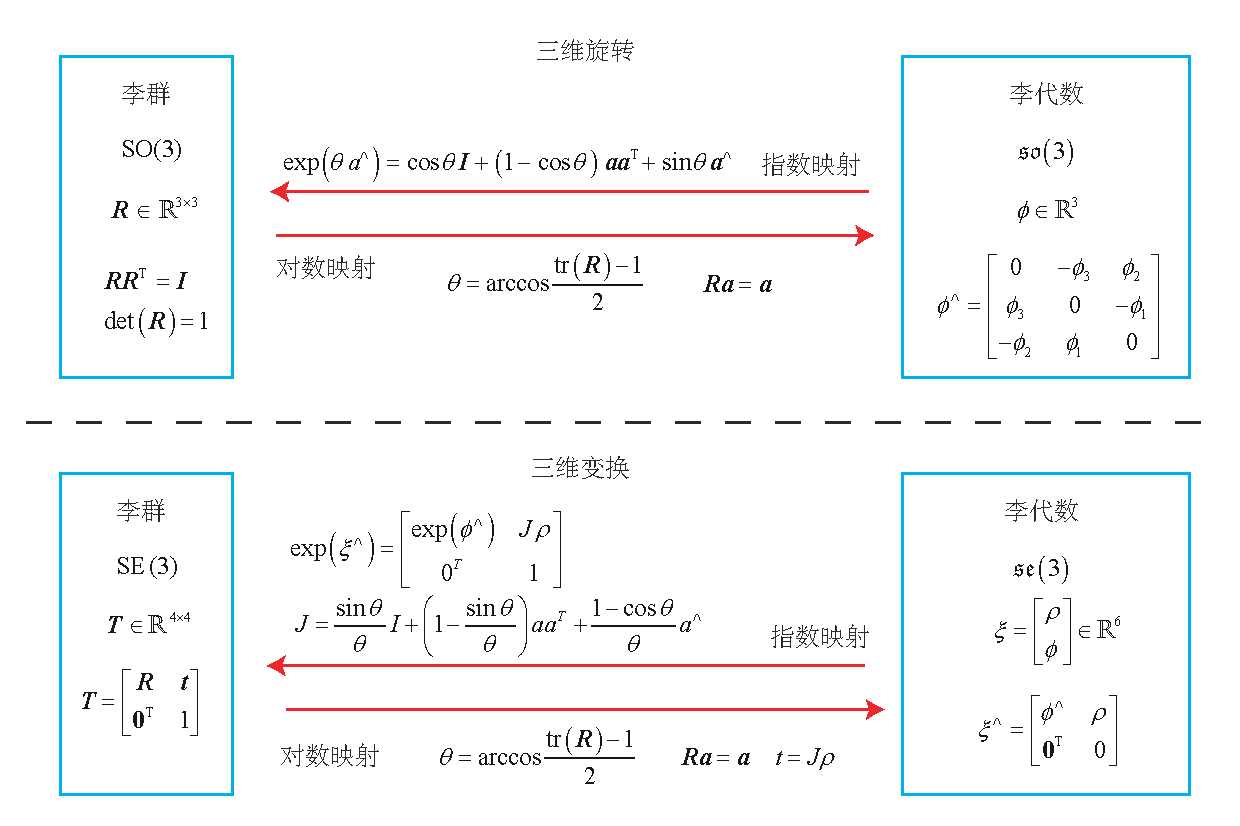
\includegraphics[width=1.0\textwidth]{lieGroup/liegroupandAlgebra.pdf}
	\caption{$\mathrm{SO}(3),\mathrm{SE}(3),\mathfrak{so}(3), \mathfrak{se}(3)$的对应关系。}
	\label{fig:liegroupandAlgebra}
\end{figure}

\clearpage

\section{李代数求导与扰动模型}
\subsection{BCH公式与近似形式}
使用李代数的一大动机是进行优化,而在优化过程中导数是非常必要的信息(我们会在第6讲详细介绍)。下面来考虑一个问题。虽然我们已经清楚了$\mathrm{SO}(3)$和$\mathrm{SE}(3)$上的李群与李代数关系,但是,当在$\mathrm{SO}(3)$中完成两个矩阵乘法时,李代数中$\mathfrak{so}(3)$上发生了什么改变呢?反过来说,当$\mathfrak{so}(3)$上做两个李代数的加法时,$\mathrm{SO}(3)$上是否对应着两个矩阵的乘积?如果成立,相当于:
\[
\exp \left( {\boldsymbol{\phi} _1^ \wedge } \right)\exp \left( {\boldsymbol{\phi} _2^ \wedge } \right) = \exp \left( {{{\left( {{\boldsymbol{\phi} _1} + {\boldsymbol{\phi} _2}} \right)}^ \wedge }} \right) ?
\]

如果$\boldsymbol{\phi}_1, \boldsymbol{\phi}_2$为标量,那显然该式成立;但此处我们计算的是\textbf{矩阵}的指数函数,而非标量的指数。换言之,我们在研究下式是否成立:
\[
	\ln \left( \exp \left( \bm{A} \right) \exp \left( \bm{B} \right) \right) = \bm{A} + \bm{B} \; ?
\]

很遗憾,该式在矩阵时并不成立。两个李代数指数映射乘积的完整形式,由Baker-Campbell-Hausdorff公式(BCH公式)\footnote{ 参见\url{https://en.wikipedia.org/wiki/Baker-Campbell-Hausdorff\_formula}。}给出。由于其完整形式较复杂,我们只给出其展开式的前几项:
\begin{equation}
\ln \left( {\exp \left( \bm{A} \right)\exp \left( \bm{B} \right)} \right) = \bm{A} + \bm{B} + \frac{1}{2}\left[ {\bm{A}, \bm{B}} \right] + \frac{1}{{12}}\left[ {\bm{A},\left[ {\bm{A}, \bm{B}} \right]} \right] - \frac{1}{{12}}\left[ {\bm{B},\left[ {\bm{A},\bm{B}} \right]} \right] +  \cdots 
\end{equation}
其中$[]$为李括号。BCH公式告诉我们,当处理两个矩阵指数之积时,它们会产生一些由李括号组成的余项。特别地,考虑$\mathrm{SO}(3)$上的李代数$\ln { \left( {\exp \left( { \boldsymbol{\phi} _1^ \wedge } \right)\exp \left( {\boldsymbol{\phi} _2^ \wedge } \right)} \right) ^ \vee }$,当$\boldsymbol{\phi_1}$或$\boldsymbol{\phi_2}$为小量时,小量二次以上的项都可以被忽略掉。此时,BCH拥有线性近似表达\footnote{对BCH具体形式和近似表达的具体推导,本书不作讨论,请参考文献\cite{Barfoot2016}。}:
\begin{equation}
 \ln { \left( {\exp \left( { \boldsymbol{\phi} _1^ \wedge } \right)\exp \left( {\boldsymbol{\phi} _2^ \wedge } \right)} \right) ^ \vee } \approx \left\{ 
 \begin{array}{l}
 {\bm{J}_l}{\left( {{\boldsymbol{\phi} _2}} \right)^{ - 1}}{ \boldsymbol{\phi} _1} + {\boldsymbol{\phi} _2} \quad \text{当} \boldsymbol{\phi}_1 \text{为小量},\\
 {\bm{J}_r}{\left( {{\boldsymbol{\phi} _1}} \right)^{ - 1}}{\boldsymbol{\phi} _2} + {\boldsymbol{\phi} _1} \quad \text{当} \boldsymbol{\phi}_2 \text{为小量}.
 \end{array} \right.
\end{equation}

以第一个近似为例。该式告诉我们,当对一个旋转矩阵$\bm{R}_2$(李代数为$\boldsymbol{\phi}_2$)左乘一个微小旋转矩阵$\bm{R}_1$(李代数为$\boldsymbol{\phi} _1$)时,可以近似地看作,在原有的李代数$\boldsymbol{\phi}_2$上加上了一项${\bm{J}_l}{\left( {{\boldsymbol{\phi} _2}} \right)^{ - 1}}{ \boldsymbol{\phi} _1}$。同理,第二个近似描述了右乘一个微小位移的情况。于是,李代数在BCH近似下,分成了左乘近似和右乘近似两种,在使用时我们须注意使用的是左乘模型还是右乘模型。

本书以左乘为例。左乘BCH近似雅可比$\bm{J}_l$事实上就是式~\eqref{eq:lieAlgebraJacobian}~的内容:
\begin{equation} 
{ \bm{J}_l} = \bm{J} = \frac{{\sin \theta }}{\theta } \bm{I} + \left( {1 - \frac{{\sin \theta }}{\theta }} \right) \bm{a} { \bm{a}^\mathrm{T}} + \frac{{1 - \cos \theta }}{\theta }{ \bm{a}^ \wedge}.
\end{equation}

它的逆为:
\begin{equation}
\bm{J}_l^{ - 1} = \frac{\theta }{2}\cot \frac{\theta }{2} \bm{I} + \left( {1 - \frac{\theta }{2}\cot \frac{\theta }{2}} \right) \bm{a} {\bm{a}^\mathrm{T}} - \frac{\theta }{2}{ \bm{a}^ \wedge }.
\end{equation}
而右乘雅可比仅需要对自变量取负号即可:
\begin{equation}
\bm{J}_r(\boldsymbol{\phi}) =\bm{J}_l(-\boldsymbol{\phi}) .
\end{equation}

这样,我们就可以谈论李群乘法与李代数加法的关系了。

为了方便读者理解,我们重新叙述一下BCH近似的意义。假定对某个旋转$\bm{R}$,对应的李代数为$\boldsymbol{\phi}$。我们给它左乘一个微小旋转,记作$\Delta \bm{R}$,对应的李代数为$\Delta \boldsymbol{\phi}$。那么,在李群上,得到的结果就是$ \Delta \bm{R} \cdot \bm{R}$,而在李代数上,根据BCH近似,为$\bm{J}_l^{-1} (\boldsymbol{\phi}) \Delta \boldsymbol{\phi} + \boldsymbol{\phi}$。合并起来,可以简单地写成:
\begin{equation}
\exp \left( {\Delta { \boldsymbol{\phi} ^ \wedge }} \right)\exp \left( {{ \boldsymbol{\phi} ^ \wedge }} \right) = \exp \left( {{{\left( { \boldsymbol{\phi}  + \bm{J}_l^{ - 1}\left( \boldsymbol{\phi}  \right)\Delta \boldsymbol{\phi} } \right)}^ \wedge }} \right).
\end{equation}

反之,如果我们在李代数上进行加法,让一个$\boldsymbol{\phi}$加上$\Delta \boldsymbol{\phi}$,那么可以近似为李群上带左右雅可比的乘法:
\begin{equation}
\exp \left( {{{\left( { \boldsymbol{\phi}  + \Delta \boldsymbol{\phi} } \right)}^ \wedge }} \right) = \exp \left( {{{\left( {{ \bm{J}_l}\Delta \boldsymbol{\phi} } \right)}^ \wedge }} \right)\exp \left( {{ \boldsymbol{\phi} ^ \wedge }} \right) = \exp \left( {{\boldsymbol{\phi} ^ \wedge }} \right)\exp \left( {{{\left( {{\bm{J}_r}\Delta \boldsymbol{\phi} } \right)}^ \wedge }} \right).
\end{equation}

这就为之后李代数上做微积分提供了理论基础。同样地,对于$\mathrm{SE}(3)$,亦有类似的BCH近似:
\begin{equation}
\exp \left( {\Delta {\boldsymbol{\xi} ^ \wedge }} \right)\exp \left( {{ \boldsymbol{\xi} ^ \wedge }} \right) \approx \exp \left( {{{\left( {{ \bm{\mathcal{J}}_l^{-1} }\Delta \boldsymbol{\xi}  + \boldsymbol{\xi} } \right)}^ \wedge }} \right),
\end{equation}
\begin{equation}
\exp \left( {{ \boldsymbol{\xi} ^ \wedge }} \right) \exp \left( {\Delta {\boldsymbol{\xi} ^ \wedge }} \right)  \approx \exp \left( {{{\left( {{ \bm{\mathcal{J}}_r^{-1} }\Delta \boldsymbol{\xi}  + \boldsymbol{\xi} } \right)}^ \wedge }} \right).
\end{equation}

这里$\bm{\mathcal{J}}_l$形式比较复杂,它是一个$6 \times 6$的矩阵,读者可以参考文献\cite{Barfoot2016}中式(7.82)和(7.83)的内容。由于我们在计算中没有用到该雅可比,故这里略去它的实际形式。

\enlargethispage{9pt}
\subsection{$\mathrm{SO}(3)$李代数上的求导}
下面来讨论一个带有李代数的函数,如何关于该李代数求导的问题。该问题有很强的实际背景。在SLAM中,我们要估计一个相机的位置和姿态,该位姿是由$\mathrm{SO}(3)$上的旋转矩阵或$\mathrm{SE}(3)$上的变换矩阵描述的。不妨设某个时刻小萝卜的位姿为$\bm{T}$。它观察到了一个世界坐标位于$\bm{p}$的点,产生了一个观测数据$\bm{z}$。那么,由坐标变换关系知:
%\clearpage
\begin{equation}
\bm{z} = \bm{T} \bm{p} + \bm{w}.
\end{equation}
其中$\bm{w}$为随机噪声。由于它的存在,$\bm{z}$往往不可能精确地满足$\bm{z} = \bm{T} \bm{p}$的关系。所以,我们通常会计算理想的观测与实际数据的误差:
\begin{equation}
\bm{e} = \bm{z} - \bm{T} \bm{p}.
\end{equation}

假设一共有$N$个这样的路标点和观测,于是就有$N$个上式。那么,对小萝卜的位姿估计,相当于是寻找一个最优的$\bm{T}$,使得整体误差最小化:
\begin{equation}
\mathop {\min }\limits_{\bm{T}} J(\bm{T} ) = \sum_{i=1}^{N} \left\| {\bm{z}_i - \bm{Tp}_i} \right\|^2_2.
\end{equation}

求解此问题,需要计算目标函数$J$关于变换矩阵$\bm{T}$的导数。我们把具体的算法留到后面再讲。这里的重点是,\textbf{我们经常会构建与位姿有关的函数,然后讨论该函数关于位姿的导数,以调整当前的估计值}。然而,$\mathrm{SO}(3),\mathrm{SE}(3)$上并没有良好定义的加法,它们只是群。如果我们把$\bm{T}$当成一个普通矩阵来处理优化,那就必须对它加以约束。而从李代数角度来说,由于李代数由向量组成,具有良好的加法运算。因此,使用李代数解决求导问题的思路分为两种:

\begin{enumerate}
	\item 用李代数表示姿态,然后根据李代数加法来对\textbf{李代数求导}。
	\item 对李群\textbf{左乘}或\textbf{右乘}微小扰动,然后对该\textbf{扰动求导},称为左扰动和右扰动模型。
\end{enumerate}

第一种方式对应到李代数的求导模型,而第二种则对应到扰动模型。下面来讨论这两种思路的异同。

\subsection{李代数求导}
首先,考虑$\mathrm{SO}(3)$上的情况。假设我们对一个空间点$\bm{p}$进行了旋转,得到了$\bm{R} \bm{p}$。现在,要计算旋转之后点的坐标相对于旋转的导数,我们非正式地记为\footnote{请注意这里并不能按照矩阵微分来定义导数,这只是一个记号。}:
\[
\frac{{\partial \left( {\bm{Rp}} \right)}}{{\partial \bm{R}}}.
\]
由于$\mathrm{SO}(3)$没有加法,所以该导数无法按照导数的定义进行计算。设$\bm{R}$对应的李代数为$\boldsymbol{\phi}$,我们转而计算\footnote{严格说来,在矩阵微分中,只能求行向量关于列向量的导数,所得结果是一个矩阵。但本书写成列向量对列向量的导数,读者可以认为先对分子进行转置,再对最后结果进行转置。这使得式子变得简洁,不然我们就不得不给每一行的分子加一个转置符号。在这种意义下,可以认为$\mathrm{d}(\bm{Ax})/\mathrm{d}\bm{x} = \bm{A}$。}:
\[ \frac{{\partial \left( {\exp \left( \boldsymbol{\phi} ^ \wedge \right) \bm{p}} \right)}}{{\partial \boldsymbol{\phi} }}. \]

%\clearpage
按照导数的定义,有:
\begin{align*}
\frac{{\partial \left( {\exp \left( {{ \boldsymbol{\phi} ^ \wedge }} \right) \bm{p}} \right)}}{{\partial \boldsymbol{\phi} }} &= \mathop {\lim }\limits_{\delta \boldsymbol{\phi}  \to \bm{0}} \frac{{\exp \left( {{{\left( {\boldsymbol{\phi}  + \delta \boldsymbol{\phi} } \right)}^ \wedge }} \right) \bm{p} - \exp \left( {{\boldsymbol{\phi} ^ \wedge }} \right)\bm{p}}}{{\delta \boldsymbol{\phi} }}\\
& = \mathop {\lim }\limits_{\delta \boldsymbol{\phi}  \to \bm{0}} \frac{{\exp \left( {{{\left( {{\bm{J}_l}\delta \boldsymbol{\phi} } \right)}^ \wedge }} \right)\exp \left( {{\boldsymbol{\phi} ^ \wedge }} \right) \bm{p} - \exp \left( {{\boldsymbol{\phi} ^ \wedge }} \right) \bm{p}}}{{\delta \boldsymbol{\phi} }}\\
&= \mathop {\lim }\limits_{\delta \boldsymbol{\phi}  \to \bm{0}} \frac{{\left( { \bm{I} + {{\left( {{ \bm{J}_l}\delta \boldsymbol{\phi} } \right)}^ \wedge }} \right)\exp \left( {{\boldsymbol{\phi} ^ \wedge }} \right) \bm{p} - \exp \left( {{\boldsymbol{\phi} ^ \wedge }} \right)\bm{p}}}{{\delta \boldsymbol{\phi} }}\\
&= \mathop {\lim }\limits_{\delta \boldsymbol{\phi}  \to \bm{0}} \frac{{{{\left( {{\bm{J}_l}\delta \boldsymbol{\phi} } \right)}^ \wedge }\exp \left( {{\boldsymbol{\phi} ^ \wedge }} \right)\bm{p}}}{{\delta \boldsymbol{\phi} }}\\
&= \mathop {\lim }\limits_{\delta \boldsymbol{\phi}  \to \bm{0}} \frac{{ - {{\left( {\exp \left( {{\boldsymbol{\phi} ^ \wedge }} \right)\bm{p}} \right)}^ \wedge }{\bm{J}_l}\delta \boldsymbol{\phi} }}{{\delta \boldsymbol{\phi}}} =  - {\left( {\bm{Rp}} \right)^ \wedge }{\bm{J}_l}.
\end{align*}

第2行的近似为BCH线性近似,第3行为泰勒展开舍去高阶项后的近似(但由于取了极限,可以写等号),第4行至第5行将反对称符号看作叉积,交换之后变号。于是,我们推导出了旋转后的点相对于李代数的导数:
\begin{equation}
\frac{{\partial \left( { \bm{Rp}} \right)}}{{\partial \boldsymbol{\phi} }} = {\left( { - \bm{Rp}} \right)^ \wedge }{\bm{J}_l}.
\end{equation}

不过,由于这里仍然含有形式比较复杂的$\bm{J}_l$,我们不太希望计算它。而下面要讲的扰动模型则提供了更简单的导数计算方式。

\subsection{扰动模型(左乘)}
另一种求导方式是对$\bm{R}$进行一次扰动$\Delta \bm{R}$,看结果相对于扰动的变化率。这个扰动可以乘在左边也可以乘在右边,最后结果会有一点儿微小的差异,我们以左扰动为例。设左扰动$\Delta \bm{R}$对应的李代数为$\boldsymbol{\varphi}$。然后,对$\boldsymbol{\varphi}$求导,即:
\begin{equation}
\frac{{\partial \left( {\bm{Rp}} \right)}}{{\partial \boldsymbol{\varphi} }} = \mathop {\lim }\limits_{\boldsymbol{\varphi}  \to \bm{0}} \frac{{\exp \left( {{\boldsymbol{\varphi} ^ \wedge }} \right)\exp \left( {{\boldsymbol{\phi} ^ \wedge }} \right)\bm{p} - \exp \left( {{\boldsymbol{\phi} ^ \wedge }} \right)\bm{p}}}{\boldsymbol{\varphi} }.
\end{equation}

该式的求导比上面更为简单:
\begin{align*}
\frac{{\partial \left( {\bm{Rp}} \right)}}{{\partial \boldsymbol{\varphi} }} &= \mathop {\lim }\limits_{\boldsymbol{\varphi}  \to \bm{0}} \frac{{\exp \left( {{\boldsymbol{\varphi} ^ \wedge }} \right)\exp \left( {{\boldsymbol{\phi} ^ \wedge }} \right)\bm{p} - \exp \left( {{\boldsymbol{\phi} ^ \wedge }} \right)\bm{p}}}{ \boldsymbol{\varphi} }\\
&= \mathop {\lim }\limits_{\boldsymbol{\varphi } \to \bm{0}} \frac{{\left( {\bm{I} + {\boldsymbol{\varphi }^ \wedge }} \right)\exp \left( {{\boldsymbol{\phi} ^ \wedge }} \right)\bm{p} - \exp \left( {{\boldsymbol{\phi} ^ \wedge }} \right)\bm{p}}}{\boldsymbol{\varphi} }\\
&= \mathop {\lim }\limits_{\boldsymbol{\varphi}  \to \bm{0}} \frac{{{\boldsymbol{\varphi} ^ \wedge }\bm{Rp}}}{\boldsymbol{\varphi} } = \mathop {\lim }\limits_{\boldsymbol{\varphi}  \to \bm{0}} \frac{{ - {{\left( \bm{Rp} \right)}^ \wedge }\boldsymbol{\varphi} }}{\boldsymbol{\varphi} } =  - {\left( \bm{Rp} \right)^ \wedge }.
\end{align*}

可见,相比于直接对李代数求导,省去了一个雅可比$\bm{J}_l$的计算。这使得扰动模型更为实用。请读者务必理解这里的求导运算,这在位姿估计当中具有重要的意义。

\subsection{$\mathrm{SE}(3)$上的李代数求导}
\label{sec:se3-diff}
最后,我们给出$\mathrm{SE}(3)$上的扰动模型,而直接李代数上的求导就不再介绍了。假设某空间点$\bm{p}$经过一次变换$\bm{T}$(对应李代数为$\boldsymbol{\xi}$),得到$\bm{Tp}$\footnote{请注意为了使乘法成立,$\bm{p}$必须使用齐次坐标。}。现在,给$\bm{T}$左乘一个扰动$\Delta \bm{T} = \exp \left( \delta \boldsymbol{\xi}^\wedge  \right)$,我们设扰动项的李代数为$\delta \boldsymbol{\xi} = [\delta \boldsymbol{\rho}, \delta \boldsymbol{\phi}]^\mathrm{T}$,那么:
\begin{align*}
\frac{{\partial \left( \bm{Tp} \right)}}{{\partial \delta \boldsymbol{\xi}}} &= \mathop {\lim }\limits_{\delta \boldsymbol{\xi}  \to \bm{0}} \frac{{\exp \left( {\delta {\boldsymbol{\xi} ^ \wedge }} \right)\exp \left( {{\boldsymbol{\xi} ^ \wedge }} \right) \bm{p} - \exp \left( {{\boldsymbol{\xi} ^ \wedge }} \right) \bm{p} }}{{\delta \boldsymbol{\xi} }}\\
&= \mathop {\lim }\limits_{\delta \boldsymbol{\xi}  \to \bm{0}} \frac{{\left( { \bm{I} + \delta {\boldsymbol{\xi} ^ \wedge }} \right)\exp \left( {{\boldsymbol{\xi} ^ \wedge }} \right) \bm{p} - \exp \left( {{\boldsymbol{\xi} ^ \wedge }} \right) \bm{p} }}{{\delta {\boldsymbol{\xi} }}}\\
&= \mathop {\lim }\limits_{\delta \boldsymbol{\xi}  \to \bm{0}} \frac{{\delta {\boldsymbol{\xi} ^ \wedge }\exp \left( {{\boldsymbol{\xi} ^ \wedge }} \right) \bm{p}}}{{\delta {\boldsymbol{\xi} }}}\\
&= \mathop {\lim }\limits_{\delta \boldsymbol{\xi}  \to \bm{0}} 
\frac{{\left[ {\begin{array}{*{20}{c}}
			{\delta { \boldsymbol{\phi} ^ \wedge }}&{\delta {\boldsymbol{\rho} }}\\
			{{\bm{0}^\mathrm{T}}}&0
			\end{array}} \right]\left[ {\begin{array}{*{20}{c}}
			{\bm{Rp} + \bm{t}}\\
			1
			\end{array}} \right]}}{{\delta {\boldsymbol{\xi} }}}\\
&= \mathop {\lim }\limits_{\delta \boldsymbol{\xi}  \to \bm{0}} \frac{{\left[ {\begin{array}{*{20}{c}}
			{\delta {\boldsymbol{\phi} ^ \wedge }\left( {\bm{Rp} + \bm{t}} \right) + \delta {\boldsymbol{\rho} }}\\
			\bm{0}^\mathrm{T}
			\end{array}} \right]}}{[\delta\boldsymbol{\rho},\delta \boldsymbol{\phi}]^\mathrm{T}} = \left[ {\begin{array}{*{20}{c}}
	\bm{I} & { - {{\left( {\bm{Rp} + \bm{t}} \right)}^ \wedge }} \\
	{{\bm{0}}}^\mathrm{T} & \bm{0}^\mathrm{T}
	\end{array}} \right] \buildrel \Delta \over = {\left( \bm{Tp} \right)^ \odot }.
\end{align*}

我们把最后的结果定义成一个算符$^\odot$\footnote{我会读作“咚”,像一个石子掉在井里的声音。},它把一个齐次坐标的空间点变换成一个$4 \times 6$的矩阵。此式稍微需要解释的是矩阵求导方面的顺序,假设$\bm{a}, \bm{b}, \bm{x}, \bm{y}$都是列向量,那么在我们的符号写法下,有如下的规则:
\begin{equation}
\frac{\mathrm{\mathrm{d}}\begin{bmatrix}
\bm{a}\\
\bm{b}
\end{bmatrix}}{{\mathrm{d} \begin{bmatrix}
\bm{x}\\
\bm{y}
\end{bmatrix}}} = {\left( \frac{\mathrm{d}[\bm{a},\bm{b}]^\mathrm{T}}{{\mathrm{d}\begin{bmatrix}
\bm{x}\\
\bm{y}
\end{bmatrix}}} \right)^\mathrm{T}} = {{\begin{bmatrix}
{\frac{{\mathrm{d}\bm{a}}}{{\mathrm{d}\bm{x}}}}&{\frac{{\mathrm{d}\bm{b}}}{{\mathrm{d}\bm{x}}}}\\
{\frac{{\mathrm{d}\bm{a}}}{{\mathrm{d}\bm{y}}}}&{\frac{{\mathrm{d}\bm{b}}}{{\mathrm{d}\bm{y}}}}
\end{bmatrix}} ^\mathrm{T}} = {\begin{bmatrix}
{\frac{{\mathrm{d}\bm{a}}}{{\mathrm{d}\bm{x}}}}&{\frac{{\mathrm{d}\bm{a}}}{{\mathrm{d}\bm{y}}}}\\
{\frac{{\mathrm{d}\bm{b}}}{{\mathrm{d}\bm{x}}}}&{\frac{{\mathrm{d}\bm{b}}}{{\mathrm{d}\bm{y}}}}
\end{bmatrix}}
\end{equation}

至此,我们已经介绍了李群李代数上的微分运算。之后的章节中,我们将应用这些知识去解决实际问题。关于李群李代数的某些重要数学性质,我们作为习题留给读者。

\section{实践:Sophus}
\subsection{Sophus的基本使用方法}
我们已经介绍了李代数的入门知识,现在是通过实践演练巩固一下所学知识的时候了。我们来讨论如何在程序中操作李代数。在第3讲中,我们看到Eigen提供了几何模块,但没有提供李代数的支持。一个较好的李代数库是Strasdat维护的Sophus库\footnote{最早提出李代数的是Sophus Lie,这个库就以他的名字命名了。}。Sophus库支持本章主要讨论的$\mathrm{SO}(3)$和$\mathrm{SE}(3)$,此外还含有二维运动$\mathrm{SO}(2), \mathrm{SE}(2)$以及相似变换$\mathrm{Sim}(3)$的内容。它是直接在Eigen基础上开发的,我们不需要安装额外的依赖库。读者可以直接从GitHub上获取Sophus,或者,在本书的代码目录slambook/3rdparty下也提供了Sophus源代码。由于历史原因,Sophus早期版本只提供了双精度的李群/李代数类。后续版本改写成了模板类。模板类的Sophus中可以使用不同精度的李群/李代数,但同时增加了使用难度。在本书第二版中,我们使用\textbf{带模板}的Sophus库。本书的3rdparty中提供的Sophus是\textbf{模板}版本,它应该在你下载本书代码的时候就已经复制下来了。Sophus本身亦是一个cmake工程。想必你已经了解如何编译cmake工程了,这里不再赘述。Sophus库只需编译即可,无须安装。

下面来演示一下Sophus库中的SO(3)和SE(3)运算:

\begin{lstlisting}[language=c++,caption=slambook/ch4/useSophus.cpp]
#include <iostream>
#include <cmath>
#include <Eigen/Core>
#include <Eigen/Geometry>
#include "sophus/se3.hpp"

using namespace std;
using namespace Eigen;

/// 本程序演示sophus的基本用法
int main(int argc, char **argv) {
	// 沿Z轴转90度的旋转矩阵
	Matrix3d R = AngleAxisd(M_PI / 2, Vector3d(0, 0, 1)).toRotationMatrix();
	// 或者四元数
	Quaterniond q(R);
	Sophus::SO3d SO3_R(R);              // Sophus::SO3d可以直接从旋转矩阵构造
	Sophus::SO3d SO3_q(q);              // 也可以通过四元数构造
	// 二者是等价的
	cout << "SO(3) from matrix:\n" << SO3_R.matrix() << endl;
	cout << "SO(3) from quaternion:\n" << SO3_q.matrix() << endl;
	cout << "they are equal" << endl;
	
	// 使用对数映射获得它的李代数
	Vector3d so3 = SO3_R.log();
	cout << "so3 = " << so3.transpose() << endl;
	// hat 为向量到反对称矩阵
	cout << "so3 hat=\n" << Sophus::SO3d::hat(so3) << endl;
	// 相对的,vee为反对称到向量
	cout << "so3 hat vee= " << Sophus::SO3d::vee(Sophus::SO3d::hat(so3)).transpose() << endl;
	
	// 增量扰动模型的更新
	Vector3d update_so3(1e-4, 0, 0); //假设更新量为这么多
	Sophus::SO3d SO3_updated = Sophus::SO3d::exp(update_so3) * SO3_R;
	cout << "SO3 updated = \n" << SO3_updated.matrix() << endl;
	
	cout << "*******************************" << endl;
	// 对SE(3)操作大同小异
	Vector3d t(1, 0, 0);           // 沿X轴平移1
	Sophus::SE3d SE3_Rt(R, t);           // 从R,t构造SE(3)
	Sophus::SE3d SE3_qt(q, t);            // 从q,t构造SE(3)
	cout << "SE3 from R,t= \n" << SE3_Rt.matrix() << endl;
	cout << "SE3 from q,t= \n" << SE3_qt.matrix() << endl;
	// 李代数se(3) 是一个六维向量,方便起见先typedef一下
	typedef Eigen::Matrix<double, 6, 1> Vector6d;
	Vector6d se3 = SE3_Rt.log();
	cout << "se3 = " << se3.transpose() << endl;
	// 观察输出,会发现在Sophus中,se(3)的平移在前,旋转在后.
	// 同样的,有hat和vee两个算符
	cout << "se3 hat = \n" << Sophus::SE3d::hat(se3) << endl;
	cout << "se3 hat vee = " << Sophus::SE3d::vee(Sophus::SE3d::hat(se3)).transpose() << endl;
	
	// 最后,演示一下更新
	Vector6d update_se3; //更新量
	update_se3.setZero();
	update_se3(0, 0) = 1e-4d;
	Sophus::SE3d SE3_updated = Sophus::SE3d::exp(update_se3) * SE3_Rt;
	cout << "SE3 updated = " << endl << SE3_updated.matrix() << endl;
	
	return 0;
}
\end{lstlisting}

该演示程序分为两部分。前半部分介绍$\mathrm{SO}(3)$上的操作,后半部分则为$\mathrm{SE}(3)$。我们演示了如何构造$\mathrm{SO}(3),\mathrm{SE}(3)$对象,对它们进行指数、对数映射,以及当知道更新量后,如何对李群元素进行更新。如果读者切实理解了本讲内容,那么这个程序对你来说应该没有什么难度。为了编译它,请在CMakeLists.txt里添加以下几行:

\begin{lstlisting}[caption=slambook/ch4/useSophus/CMakeLists.txt]
# 为使用 sophus,需要使用 find_package 命令找到它
find_package( Sophus REQUIRED )
include_directories( ${Sophus_INCLUDE_DIRS} )

add_executable( useSophus useSophus.cpp )
\end{lstlisting}

find\_package命令是cmake提供的寻找某个库的头文件与库文件的指令。如果cmake能够找到它,就会提供头文件和库文件所在的目录的变量。在Sophus这个例子中,就是Sophus\_INCLUDE\_DIRS。基于模板的Sophus库和Eigen一样,是仅含头文件而没有源文件的。根据它们,我们就能将Sophus库引入自己的cmake工程了。请读者自行查看此程序的输出信息,它与我们之前的推导是一致的。

\subsection{例子:评估轨迹的误差}
在实际工程中,我们经常需要评估一个算法的估计轨迹与真实轨迹的差异,来评价算法的精度。真实轨迹往往通过某些更高精度的系统获得,而估计估计则是待评价的算法计算得到。上一讲我们演示了如何显示存储在文件中的某条轨迹,本节我们来考虑如何计算两条轨迹的误差。考虑一条估计轨迹$\bm{T}_{\mathrm{esti},i}$和真实轨迹$\bm{T}_{\mathrm{gt},i}$,其中$i=1,\cdots,N$,那么我们可以定义一些误差指标来描述它们之间的差别。

误差指标可以有很多种,常见的有\textbf{绝对轨迹误差}(Absolute Trajectory Error, ATE),形如:
\begin{equation}
\mathrm{ATE}_{\mathrm{all}} = \sqrt{ \frac{1}{N} \sum_{i=1}^N \| \log( \bm{T}_{\mathrm{gt},i}^{-1} \bm{T}_{\mathrm{esti},i} )^{\vee} \|_2^2},
\end{equation}
这实际上是每个位姿李代数的\textbf{均方根误差}(Root-Mean-Squared Error, RMSE)。这种误差可以刻画两条轨迹的旋转和平移误差。同时,也有的文献仅考虑平移误差\cite{Sturm2012},从而可以定义\textbf{绝对平移误差}(Average Translational Error):
\begin{equation}
	\mathrm{ATE}_{\mathrm{trans}} = \sqrt{ \frac{1}{N} \sum_{i=1}^N \| \mathrm{trans}( \bm{T}_{\mathrm{gt},i}^{-1} \bm{T}_{\mathrm{esti},i} ) \|_2^2},
\end{equation}
其中$\mathrm{trans}$表示取括号内部变量的平移部分。因为从整条轨迹上来看,旋转出现误差后,随后的轨迹在平移上也会出现误差,所以两种指标在实际当中都适用。

除此之外,也可以定义相对的误差。例如考虑$i$时刻到$i+\Delta t$时刻的运动,那么相对位姿误差(Relative Pose Error, RPE)可定义为:
\begin{equation}
\mathrm{RPE}_{\mathrm{all}} = \sqrt{ \frac{1}{N-\Delta t} \sum_{i=1}^{N-\Delta t} \| \log \left( \left(\bm{T}_{\mathrm{gt},i}^{-1} \bm{T}_{\mathrm{gt},i+\Delta t} )\right)^{-1} \left(\bm{T}_{\mathrm{esti},i}^{-1} \bm{T}_{\mathrm{esti},i+\Delta t}\right)\right)^{\vee} \|_2^2},
\end{equation}
同样地,亦可只取平移部分:
\begin{equation}
\mathrm{RPE}_{\mathrm{trans}} = \sqrt{ \frac{1}{N-\Delta t} \sum_{i=1}^{N-\Delta t} \| \mathrm{trans} \left( \left(\bm{T}_{\mathrm{gt},i}^{-1} \bm{T}_{\mathrm{gt},i+\Delta t} )\right)^{-1} \left(\bm{T}_{\mathrm{esti},i}^{-1} \bm{T}_{\mathrm{esti},i+\Delta t}\right)\right) \|_2^2}.
\end{equation}

利用Sophus库,很容易实现这部分计算。下面我们演示一下绝对轨迹误差的计算。在这个例子中,我们有groundtruth.txt和estimated.txt两条轨迹,下面的代码将读取这两条轨迹,计算误差,然后显示到3D窗口中。为简洁起见,省略了画轨迹部分的代码,在上一讲中我们已经做过类似的工作。
\begin{lstlisting}[language=c++,caption=slambook/ch4/example/trajectoryError.cpp(部分)]
#include <iostream>
#include <fstream>
#include <unistd.h>
#include <pangolin/pangolin.h>
#include <sophus/se3.hpp>

using namespace Sophus;
using namespace std;

string groundtruth_file = "./example/groundtruth.txt";
string estimated_file = "./example/estimated.txt";

typedef vector<Sophus::SE3d, Eigen::aligned_allocator<Sophus::SE3d>> TrajectoryType;

void DrawTrajectory(const TrajectoryType &gt, const TrajectoryType &esti);

TrajectoryType ReadTrajectory(const string &path);

int main(int argc, char **argv) {
	TrajectoryType groundtruth = ReadTrajectory(groundtruth_file);
	TrajectoryType estimated = ReadTrajectory(estimated_file);
	assert(!groundtruth.empty() && !estimated.empty());
	assert(groundtruth.size() == estimated.size());
	
	// compute rmse
	double rmse = 0;
	for (size_t i = 0; i < estimated.size(); i++) {
		Sophus::SE3d p1 = estimated[i], p2 = groundtruth[i];
		double error = (p2.inverse() * p1).log().norm();
		rmse += error * error;
	}
	rmse = rmse / double(estimated.size());
	rmse = sqrt(rmse);
	cout << "RMSE = " << rmse << endl;
	
	DrawTrajectory(groundtruth, estimated);
	return 0;
}

TrajectoryType ReadTrajectory(const string &path) {
	ifstream fin(path);
	TrajectoryType trajectory;
	if (!fin) {
		cerr << "trajectory " << path << " not found." << endl;
		return trajectory;
	}
	
	while (!fin.eof()) {
		double time, tx, ty, tz, qx, qy, qz, qw;
		fin >> time >> tx >> ty >> tz >> qx >> qy >> qz >> qw;
		Sophus::SE3d p1(Eigen::Quaterniond(qx, qy, qz, qw), Eigen::Vector3d(tx, ty, tz));
		trajectory.push_back(p1);
	}
	return trajectory;
}
\end{lstlisting}

该程序输出的结果为2.207,图像如\autoref{fig:trajectory-compare}所示。读者也以尝试将旋转部分去掉,仅计算平移部分的误差。就这个例子来说,我们事实上已经帮助读者做了一些预处理任务,包括轨迹的时间对齐、外参预估,这些内容现在还没有讲到,我们将在以后的学习中谈论。

\begin{figure}[!ht]
	\centering
	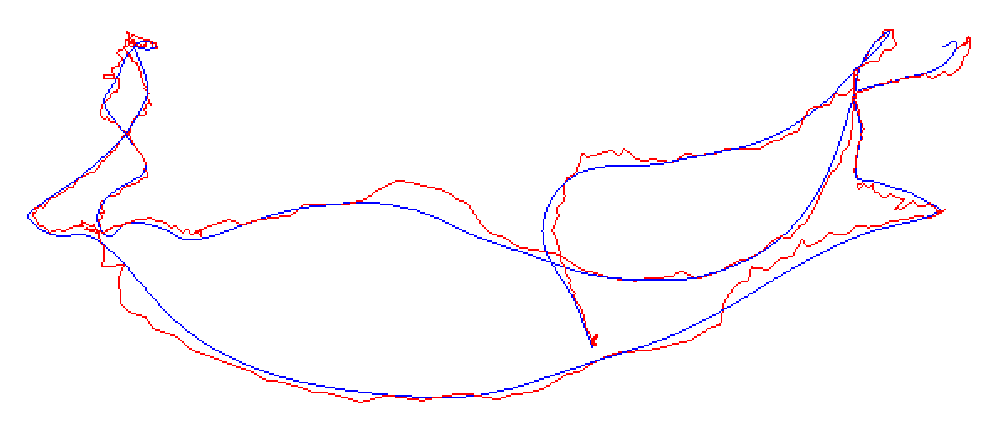
\includegraphics[width=1.0\textwidth]{lieGroup/trajectory-compare.pdf}
	\caption{计算估计轨迹与真实轨迹之间的误差。}
	\label{fig:trajectory-compare}
\end{figure}

\section{\textsuperscript{\ttfamily *}相似变换群与李代数}
最后,我们要提一下在单目视觉中使用的相似变换群$\mathrm{Sim}(3)$,以及对应的李代数$\mathfrak{sim}(3)$。如果你只对双目SLAM或RGB-D SLAM感兴趣,可以跳过本节。

我们已经介绍过单目的尺度不确定性。如果在单目SLAM中使用$\mathrm{SE}(3)$表示位姿,那么由于尺度不确定性与尺度漂移,整个SLAM过程中的尺度会发生变化,这在$\mathrm{SE}(3)$中未能体现出来。因此,在单目情况下我们一般会显式地把尺度因子表达出来。用数学语言来说,对于位于空间的点$\bm{p}$,在相机坐标系下要经过一个\textbf{相似变换},而非欧氏变换:
\begin{equation}\label{key}
\bm{p}' = \left[ {\begin{array}{*{20}{c}}
	{s\bm{R}}&\bm{t}\\
	{{\bm{0}^\mathrm{T}}}&1
	\end{array}} \right] \bm{p}
	= s\bm{R} \bm{p} + \bm{t}.
\end{equation}
在相似变换中,我们把尺度$s$表达了出来。它同时作用在$\bm{p}$的3个坐标之上,对$\bm{p}$进行了一次缩放。与$\mathrm{SO}(3)$、$\mathrm{SE}(3)$相似,相似变换亦对矩阵乘法构成群,称为相似变换群$\mathrm{Sim}(3)$:
\begin{equation}\label{key}
\mathrm{Sim}(3) = \left\{ { \bm{S} = \left[ {\begin{array}{*{20}{c}}
		{s\bm{R}}& \bm{t}\\
		{{\bm{0}^\mathrm{T}}}&1
		\end{array}} \right] \in {\mathbb{R}^{4 \times 4}}} \right\}.
\end{equation}

同样地,$\mathrm{Sim}(3)$也有对应的李代数、指数映射、对数映射等。李代数$\mathfrak{sim}(3)$元素是一个7维向量$\boldsymbol{\zeta}$。它的前6维与$\mathfrak{se}(3)$相同,最后多了一项$\sigma$。
%\clearpage
\begin{equation}
\mathfrak{sim} \left( 3 \right) = \left\{ { \boldsymbol{\zeta} | \boldsymbol{\zeta}  = \left[ \begin{array}{l}
	\boldsymbol{\rho} \\
	\boldsymbol{\phi} \\
	\sigma
	\end{array} \right] \in { \mathbb{R}^7},{ \boldsymbol{\zeta} ^ \wedge } = \left[ {\begin{array}{*{20}{c}}
		{\sigma \bm{I} + {\boldsymbol{\phi} ^ \wedge }}&\boldsymbol{\rho} \\
		{{\bm{0}^\mathrm{T}}}&0
		\end{array}} \right] \in {\mathbb{R}^{4 \times 4}}} \right\}.
\end{equation}

它比$\mathfrak{se}(3)$多了一项$\sigma$。关联$\mathrm{Sim}(3)$和$\mathfrak{sim}(3)$的仍是指数映射和对数映射。指数映射为

\begin{equation}
\exp \left( {{ \boldsymbol{\zeta} ^ \wedge }} \right) = \left[ {\begin{array}{*{20}{c}}
	{{\mathrm{e}^\sigma }\exp \left( {{ \boldsymbol{\phi} ^ \wedge }} \right)}&{ \bm{J}_s \boldsymbol{\rho} }\\
	{{\bm{0}^\mathrm{T}}}&1
	\end{array}} \right].
\end{equation}

其中$\bm{J}_s$形式为
\begin{align*}
%\begin{array}{ll}
{ \bm{J}_s} =& \frac{{{\mathrm{e}^\sigma } - 1}}{\sigma } \bm{I} + \frac{ \sigma {{\mathrm{e}^\sigma }\sin \theta  + \left( {1 - {\mathrm{e}^\sigma }\cos \theta } \right)\theta }}{{{\sigma ^2} + {\theta ^2}}}{\bm{a}^ \wedge }\\
 &+ \left( {\frac{{{\mathrm{e}^\sigma } - 1}}{\sigma } - \frac{{\left( {{\mathrm{e}^\sigma }\cos \theta  - 1} \right)\sigma  + ({\mathrm{e}^\sigma }\sin \theta )\theta }}{{{\sigma ^2} + {\theta ^2}}}} \right){\bm{a}^ \wedge }{\bm{a}^ \wedge }.
%\end{array}
\end{align*}

通过指数映射,我们能够找到李代数与李群的关系。对于李代数$\boldsymbol{\zeta}$,它与李群的对应关系为:
\begin{equation}
s=\mathrm{e}^\sigma, \; \bm{R} = \exp( \boldsymbol{\phi} ^\wedge), \; \bm{t} = \bm{J}_s \boldsymbol{\rho}.
\end{equation}

旋转部分和$\mathrm{SO}(3)$是一致的。平移部分,在$\mathfrak{se}(3)$中需要乘一个雅可比$\bm{\mathcal{J}}$,而相似变换的雅可比更复杂一些。对于尺度因子,可以看到李群中的$s$即为李代数中$\sigma$的指数函数。

$\mathrm{Sim}(3)$的BCH近似与$\mathrm{SE}(3)$是类似的。我们可以讨论一个点$\bm{p}$经过相似变换$\bm{S} \bm{p}$后,相对于$\bm{S}$的导数。同样地,存在微分模型和扰动模型两种方式,而扰动模型较为简单。我们省略推导过程,直接给出扰动模型的结果。设给予$\bm{S} \bm{p}$左侧一个小扰动$\exp( \boldsymbol{\zeta} ^\wedge )$,并求$\bm{S} \bm{p}$对于扰动的导数。因为$\bm{S} \bm{p}$是4维的齐次坐标,$\boldsymbol{\zeta}$是7维向量,该导数应该是$4 \times 7$的雅可比。为了方便起见,记$\bm{Sp}$的前3维组成向量$\bm{q}$,那么:

\begin{equation}
\frac{{\partial \bm{Sp}}}{{\partial \boldsymbol{\zeta} }} = \left[ {\begin{array}{*{20}{c}}
	\bm{I} &{ - {\bm{q}^ \wedge }}& \bm{q} \\
	{{\bm{0}^\mathrm{T}}} & {{ \bm{0}^\mathrm{T}}}&0
	\end{array}} \right].
\end{equation}

关于$\mathrm{Sim}(3)$,我们就介绍到这里。更详细的关于$\mathrm{Sim}(3)$的资料,建议读者参见文献\cite{Strasdat2012a}。


\section{小结}
本讲引入了李群$\mathrm{SO}(3)$和$\mathrm{SE}(3)$,以及它们对应的李代数$\mathfrak{so}(3)$和$\mathfrak{se}(3)$。我们介绍了位姿在它们上面的表达和转换,然后通过BCH的线性近似,就可以对位姿进行扰动并求导了。这给之后讲解位姿的优化打下了理论基础,因为我们需要经常地对某一个位姿的估计值进行调整,使它对应的误差减小。只有在弄清楚如何对位姿进行调整和更新之后,我们才能继续下一步的内容。

本讲的内容可能比较偏理论化,毕竟它不像计算机视觉那样经常有好看的图片可以展示。相比于讲解李群李代数的数学教科书,由于我们只关心实用的内容,所以讲的过程非常精简,速度也相对快了一些。请读者务必理解本讲内容,它是解决后续许多问题的基础,特别是位姿估计部分。

需要一提的是,除了李代数之外,同样也可以用四元数、欧拉角等方式表示旋转,只是后续的处理要麻烦一些。在实际应用中,也可以使用$\mathrm{SO}(3)$加上平移的方式来代替$\mathrm{SE}(3)$,从而回避一些雅可比的计算。

\section*{习题}
\begin{enumerate}
	\item 验证$\mathrm{SO}(3)$、$\mathrm{SE}(3)$和$\mathrm{Sim}(3)$关于乘法成群。
	\item 验证$( \mathbb{R}^3, \mathbb{R}, \times )$构成李代数。
	\item 验证$\mathfrak{so}(3)$和$\mathfrak{se}(3)$满足李代数要求的性质。
	\item 验证性质(4.20)和(4.21)。
	\item 证明:\[
	\bm{R} \bm{p}^\wedge \bm{R}^\mathrm{T} = (\bm{Rp})^\wedge .\]
	\item 证明:\[
	\bm{R} \exp( \bm{p}^\wedge) \bm{R}^\mathrm{T} = \exp( (\bm{Rp})^\wedge ).\] 该式称为$\mathrm{SO}(3)$上的\textbf{伴随}性质。同样地,在$\mathrm{SE}(3)$上亦有伴随性质:
	\begin{equation}
	\bm{T} \exp(\boldsymbol{\xi}^\wedge)\bm{T}^{-1} = \exp \left( \left( \mathrm{Ad}(\bm{T}) \boldsymbol{\xi} \right) ^\wedge \right),
	\end{equation}
	其中:
	\begin{equation}
	\label{eq:adjSE3}
	\mathrm{Ad} ( \bm{T} ) = \left[ {\begin{array}{*{20}{c}}
		\bm{R} &{{ \bm{t} ^ \wedge } \bm{R} }\\
		\bm{0} & \bm{R}
		\end{array}} \right]. 
	\end{equation}
	\item 仿照左扰动的推导,推导$\mathrm{SO}(3)$和$\mathrm{SE}(3)$在右扰动下的导数。
	\item 搜索cmake的find\_package指令是如何运作的。它有哪些可选的参数?为了让cmake找到某个库,需要哪些先决条件?
\end{enumerate}

% ch5 相机与图像
% !Mode:: "TeX:UTF-8"
\chapter{Cameras and Images}
\label{cpt:5}
\begin{mdframed}  
	\textbf{Goal of Study}
	\begin{enumerate}[labelindent=0em,leftmargin=1.5em]
		\item Learn the models of the pinhole camera, intrinsics, extrinsics, and distortion. 
		\item Learn how to project a spatial point into image planes. 
		\item Learn the basic image process in OpenCV. 
	\end{enumerate}
\end{mdframed} 

In the previous two lectures, we introduced how to express and optimize the robot's 6 DoF pose and partially explained the meaning of the variables and the equations of motion and observation in SLAM. This chapter will discuss ``How robots observe the outside world'', which belongs to the observation equation. In the camera-based visual SLAM, the observation mainly refers to the process of image projection.

We have seen a lot of photos in real life. A photo consists of millions of pixels in the computer, recording information about color or brightness. We will see a bundle of light reflected or emitted by an object in the three-dimensional world pass through the camera's optical center and is projected onto the camera's imaging plane. After the camera's light sensor receives the light, it produces a measurement, and we get the pixels, which form the photo we see. Can this process be described by mathematical equations? This lecture will first discuss the camera model, explain how the projection relationship is described, and the internal parameters in this projection process. At the same time, we will also give a brief introduction to the stereo and RGB-D cameras. Then, we introduce the basic operations of 2D images in OpenCV. Finally, an experiment of point cloud stitching is demonstrated to show the meaning of intrinsic and extrinsic parameters.

\newpage
\includepdf{resources/other/ch5.pdf}
\newpage
\section{Pinhole Camera Models}
The process of projecting a 3D point (in meters) to a 2D image plane (in pixels) can be described by a geometric model. Actually, several models describe this, the simplest of which is called the pinhole model. We will start with this pinhole projection. At the same time, due to the presence of the lens on the camera lens, \textit{distortion} is generated during the projection. Therefore, we will use the pinhole model plus a distortion model to describe the entire projection process.

\subsection{Pinhole Camera Geometry}
Most of us have seen the candle projection experiment in the physics class of high school: a lit candle is placed in front of a dark box, and the light of the candle is projected through a small hole in the dark box on the rear plane. Then an inverted candle image is formed on this plane. In this process, the small hole can project a candle in a three-dimensional world onto a two-dimensional imaging plane. For the same reason, we can use this simple model to explain the camera's imaging process, as shown in \autoref{fig:cameraModel}.

\begin{figure}[!ht]
	\centering
	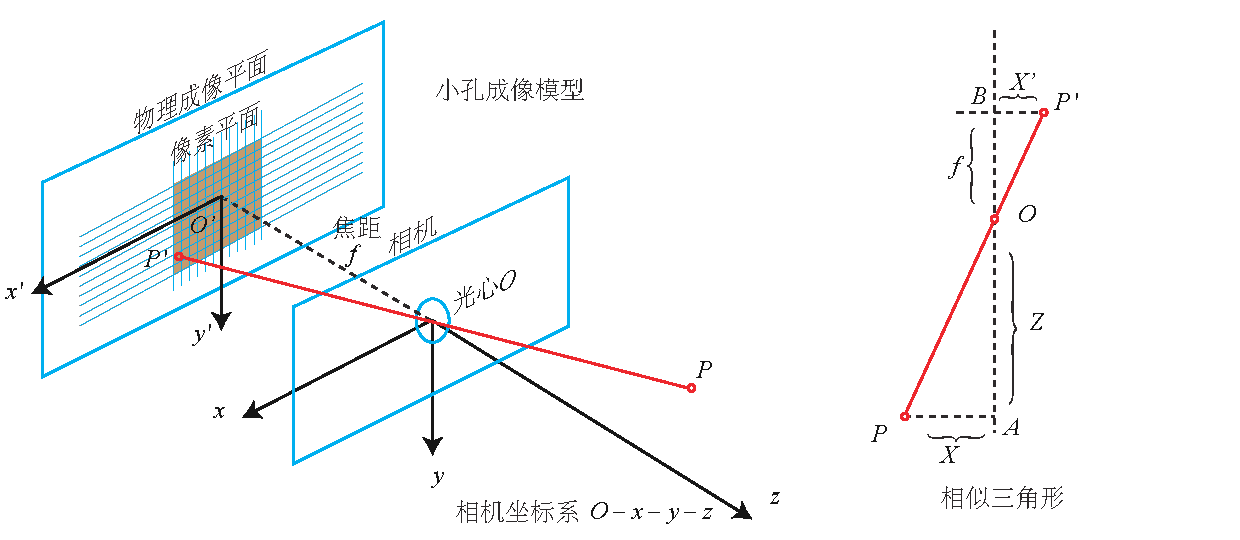
\includegraphics[width=.95\textwidth]{cameraModel/cameraModel.pdf}
	\caption{Pinhole camera model. }
	\label{fig:cameraModel}
\end{figure}

Let's take a look at the simple geometry in this model. Let $O-x-y-z$ be the camera coordinate system. Commonly we put the $z$ axis to the front of the camera, $x$ to the right, and $y$ to the down (so in this figure, we should stand on the left side to see the right side). $O$ is the camera's optical center, which is also the ``hole'' in the pinhole model. The 3D point $P$, after being projected through the hole $O$, falls on the physical imaging plane $O'-x'-y'$ and produces the image point $P'$. Let the coordinates of $P$ be $[X,Y,Z]^T$, $P'$ is $[X',Y',Z']^T$, and set the physical distance from the imaging plane to camera plane is $f$ (focal length). Then, according to the similarity of the triangles, there are:
\begin{equation}
\frac{Z}{f} = -\frac{X}{{X'}} =-\frac{Y}{{Y'}}.
\end{equation}

The negative sign indicates that the image is inverted. However, the image obtained by modern cameras is not inverted (otherwise, the usage of the camera would be very inconvenient). To make the model more realistic, we can equivalently place the imaging plane symmetrically in front of the camera, as shown by \autoref{fig:planes}. This can remove the negative sign in the formula to make it more compact:
\begin{equation}
\frac{Z}{f} = \frac{X}{{X'}} =\frac{Y}{{Y'}}.
\end{equation}

\begin{figure}[!htp]
	\centering
	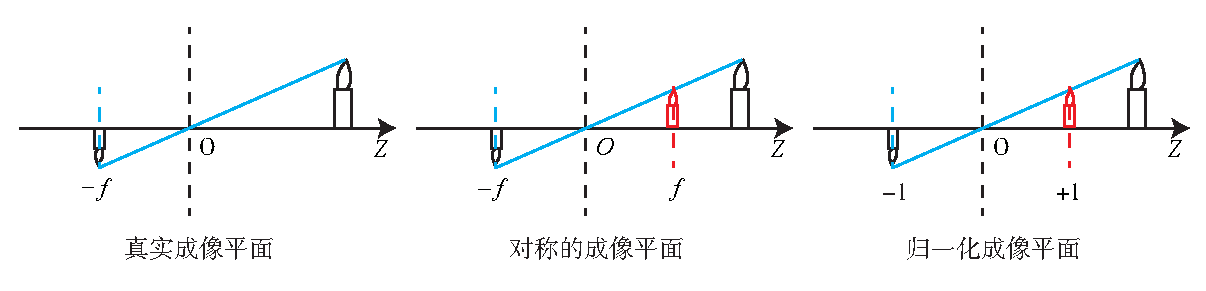
\includegraphics[width=1.0\textwidth]{cameraModel/planes.pdf}
	\caption{The real, symmetric and normalized image plane.}
	\label{fig:planes}
\end{figure}

Put $X', Y'$ to the left side:
\begin{equation}\label{eq:P2Pprime}
X' = f\frac{X}{Z}, \quad Y' = f\frac{Y}{Z}.
\end{equation}

Readers may ask why we can arbitrarily move the imaging plane to the front? In fact, this is just a mathematical approach to handle the camera projection, and most of the images captured by the camera are not upside-down. The camera's software will flip the picture for you, so what we actually get is the symmetric plane's image. Although the pin-hole image should be inverted from the physical principle since we have pre-processed the picture, it is not wrong to take the symmetric one. Therefore, without causing ambiguity, we often emit the minus symbol in the pin-hole model.


The formula~\eqref{eq:P2Pprime} describes the spatial relationship between the point $P$ and its image, where the units of all points are meters. For example, a focal length maybe 0.2 meters, and $X'$ be 0.14 meters. However, in the camera, we end up with pixels, where we need to sample and quantize the pixels on the imaging plane. To describe how the sensor converts the perceived light into image pixels, we set a pixel plane $o-u-v$ fixed on the physical imaging plane. Finally, we get \textit{pixel coordinates} of $P'$ in the pixel plane: $[u,v]^T$.

The usual definition of the pixel coordinate system \footnote{ Or image coordinate system, see section 2 of this lecture. } is: the origin $o'$ is in the upper left corner of the image, the $u$ axis is parallel to the $x$ axis, and the $v$ axis is parallel to the $y$ axis. Between the pixel coordinate system and the imaging plane, there is an apparent \textit{zoom} and a \textit{translation of the origin}. We set the pixel coordinates to scale $\alpha$ times on the $u$ axis and $\beta$ times on $v$. At the same time, the origin is translated by $[c_x, c_y]^T$. Then, the relationship between the coordinates of $P'$ and the pixel coordinate $[u,v]^T$ is:
\begin{equation}
\label{eq:project2pixel1} 
\left\{
\begin{matrix} 
u=\alpha X' + c_x\\ 
v=\beta Y' + c_y
\end{matrix}
\right. .
\end{equation}

Put it into~\eqref{eq:P2Pprime} and set $\alpha f$ as $f_x$, $\beta f$ as $f_y$:
\begin{equation}
\left\{
\begin{matrix} 
u=f_x\frac{X}{Z} + c_x\\ 
v=f_y\frac{Y}{Z} + c_y
\end{matrix}
\right. ,
\end{equation}
where $f$ is the focal length in meters, $\alpha, and \beta$ is in pixels/meter, so $f_x, f_y$ and $c_x, c_y$ are in pixels. It would be more compact to write this form as a matrix, but we need to use homogeneous coordinates on the left and non-homogeneous coordinates on the right:
\begin{equation}
\label{eq:intrinmatrix} 
\begin{pmatrix} u\\ v\\ 1 \end{pmatrix}=\frac{1}{Z}\begin{pmatrix} f_x & 0&c_x \\ 0& f_y& c_y\\ 0&0 & 1 \end{pmatrix}\begin{pmatrix} X\\ Y\\ Z \end{pmatrix} 
\buildrel \Delta \over =\frac{1}{Z} \mathbf{K} \mathbf{P}.
\end{equation}

Let's put $Z$ to the left side as in most books:
\begin{equation}
Z \begin{pmatrix} u\\ v\\ 1 \end{pmatrix}= \begin{pmatrix} f_x & 0&c_x \\ 0& f_y& c_y\\ 0&0 & 1 \end{pmatrix}\begin{pmatrix} X\\ Y\\ Z \end{pmatrix} 
\buildrel \Delta \over = \mathbf{K} \mathbf{P}.
\end{equation}

In this equation, we refer to the matrix composed of the middle quantities as the camera's inner parameter matrix (o intrinsics) $\mathbf{K}$. It is generally assumed that the camera's internal parameters are fixed after manufacturing and will not change during usage. Some camera manufacturers will tell you the intrinsics, and sometimes you need to estimate the internal parameters by yourself, which is called calibration. Because of the maturity of the calibration algorithm (such as the famous Zhang Zhengyou's calibration {\cite{Zhang1999}}), it will not be introduced here \footnote{I'm sure professor Zhang has a copy of this book now.}. 

There are internal parameters, and naturally, there must be something like ``external parameters''. In the equation ~\eqref{eq:intrinmatrix}~, we use the coordinates of $P$ in the camera coordinate system, but in fact, the coordinates of $P$ should be its world coordinates because the camera is moving (we use the symbol $\mathbf{P}_w$). It should be converted to the camera coordinate system based on the current pose of the camera. The camera's pose is described by its rotation matrix $\mathbf{R}$ and the translation vector $\mathbf{t}$. Then there are:

\begin{equation}
\label{eq:cameraprojection}
Z \mathbf{P}_{uv}=
Z \left[ \begin{array}{l}
u\\
v\\
1
\end{array} \right] = \mathbf{K} \left( {\mathbf{R}{ \mathbf{P}_w} + \mathbf{t}} \right) =  \mathbf{K} \mathbf{T} \mathbf{P}_w .
\end{equation}

Note that the latter formula implies a conversion from homogeneous to non-homogeneous coordinates (can you see it?) We use homogeneous coordinates in $\mathbf{T}\mathbf{P}$, then convert to non-homogeneous coordinates, and then multiply it by $\mathbf{K}$.  It describes the projection relationship of world coordinates to pixel coordinates of $P$. Among them, the camera's pose $\mathbf{R}, \mathbf{t}$ is also called the camera's \textit{extrinsics}. \footnote{In robots or autonomous vehicles, extrinsics is often defined as the transform between the camera coordinate system and the robot body coordinate system, describing ``where the camera is installed''.}  Compared with the intrinsic, the extrinsics may change with the camera installation and is also the target to be estimated in the SLAM if we only have a camera.

The projection process can also be viewed from another perspective. The formula ~\eqref{eq:cameraprojection} shows that we can convert a world coordinate point to the camera coordinate system first and then remove the last dimension. The depth of the point from the imaging plane of the camera is then removed, which is equivalent to the normalization on the last dimension. In this way, we get the projection of the point $P$ on the camera \textit{normalized plane}:
\begin{equation}
\left( {\mathbf{R}{\mathbf{P}_w} + \mathbf{t}} \right) = \underbrace{\left[ X,Y,Z\right]^T}_{\text{Camera Coordinates}} \to \underbrace {\left[ {X/Z,Y/Z,1} \right]^T}_{\text{Normalized Coordinates}}.
\end{equation}

The \textit{normalized coordinates} can be seen as a point in the $z=1$ plane in front of the camera \footnote{Note that in the calculation, it is necessary to check whether $Z$ is positive because the negative $Z$ can also get the point on the normalized plane by this method. However, the camera does not capture the scene behind the imaging plane. }.This $z=1$ plane is also called \textit{normalized plane}. We normalize the coordinates and then multiply them with the intrinsic matrix, yielding the pixel coordinates. We can also consider the pixel coordinates $[u,v]^T$ as the result of quantitative measurements on points on the normalized plane. If the camera coordinates are multiplied by any non-zero constant simultaneously, the normalized coordinates are the same, which means that the depth is lost during the projection process. So, in monocular vision, the pixel's depth value cannot be obtained by a single image.

\subsection{Distortion}
In order to get a larger FoV (Field-of-View), we usually add a lens in front of the camera. The addition of the lens has an influence on the propagation of light during imaging: (1) the shape of the lens may affect the propagation way of light, (2) during the mechanical assembly, the lens and the imaging plane are not entirely parallel, which also changes the projected position.

There are some mathematical models to describe the distortion caused by the shape of the lens. In the pinhole model, a straight line keeps straight when projected onto the pixel plane. However, in real photos, the camera lens tends to make a straight line in the real environment become a curve \footnote{Yes, it is no longer straight but becomes curved. If it makes an inside curve, it is called barrel-like distortion; otherwise, it is cushion-like distortion if the curve looks outward. }. The closer to the edge of the image, the more obvious this phenomenon is. Since the lenses actually produced are often center-symmetrical, this makes the irregular distortion generally radially symmetrical. They fall into two main categories: \textit{barrel-like distortion} and \textit{cushion-like distortion}, as shown by \autoref{fig:distortion}.
\begin{figure}[!t]
	\centering
	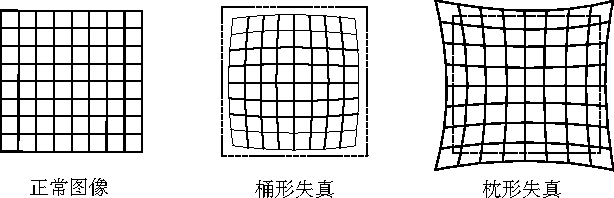
\includegraphics[width=0.7\textwidth]{cameraModel/distortion.pdf}
	\caption{The radical distortion.}
	\label{fig:distortion}
\end{figure}

In barrel distortion, the radius of pixels decreases as the optical axis's distance increases, while the cushion distortion is just the opposite. In both distortions, the line that intersects the center of the image and the optical axis remains the same.

In addition to the shape of the lens, which introduces radial distortion, \textit{tangential distortion} is introduced during assembly of the camera because the lens and the imaging surface cannot be strictly parallel, as shown by \autoref{fig:tangen}.

\begin{figure}[!t]
	\centering
	\includegraphics[width=0.7\textwidth]{cameraModel/tangen.pdf}
	\caption{Tangential distortion.}
	\label{fig:tangen}
\end{figure}
To better understand radial and tangential distortion, we describe them in a more rigorous mathematical form. Consider any point on the \textit{normalized plane}, $\mathbf{p}$, whose coordinates are $[x,y]^T$, or $[r, \theta]^T$ in the form of polar coordinates, where $r$ represents the distance between the point $\mathbf{p}$ and the origin of the coordinate system, and $\theta$ represents the angle to the horizontal axis. Radial distortion can be seen as a change in the coordinate point along the length, that is, its radius from the origin. Tangential distortion can be seen as a change in the coordinate point along the tangential direction, which means that the horizontal angle has changed. It is generally assumed that these distortions are polynomial, namely:
\begin{equation}
\label{eq:distortion} 
\begin{matrix}
x_\mathrm{distorted} = x(1+k_1r^2+k_2r^4+k_3r^6)\\
y_\mathrm{distorted} = y(1+k_1r^2+k_2r^4+k_3r^6)
\end{matrix},
\end{equation}
where $[x_\mathrm{distorted}, y_\mathrm{distorted}]^T$ is the \textit{normalized coordinates} of the point after distortion. On the other hand, for \textit{tangential distortion}, we can use the other two parameters $p_1,p_2$ to describe it:
\begin{equation}
\label{eq:tangen} 
\begin{matrix}
x_\mathrm{distorted} = x+2p_1xy+p_2(r^2+2x^2)\\
y_\mathrm{distorted} = y+p_1(r^2+2y^2)+2p_2xy
\end{matrix}. 
\end{equation}
Putting~\eqref{eq:distortion} and~\eqref{eq:tangen} together we get a joint model with 5 distortion coefficients. The complete form is:
\begin{equation}
\left\{\begin{matrix} x_\mathrm{distorted} =x(1+k_1r^2+k_2r^4+k_3r^6)+2p_1xy+p_2(r^2+2x^2)\\ 
y_\mathrm{distorted} = y(1+k_1r^2+k_2r^4+k_3r^6)+p_1(r^2+2y^2)+2p_2xy
\end{matrix}\right. .
\end{equation}

In the above process of correcting distortion, we used 5 distortion coefficients. In practical applications, you can flexibly choose to number of parameters, for example, only selecting $k_1, p_1, p_2$, or use $k_1, k_2, p_1, p_2$, etc.

This section models the camera's imaging process using a pinhole model and described the radial and tangential distortions caused by the lens. Researchers have proposed many other models in the existing imaging system, such as the affine model and perspective model, and there are many different types of distortion. In most visual SLAM systems, pinhole and rad-tan distortion models are sufficient, so we will not describe the other ones.

It is worth mentioning that there are two ways of undistortion (or correction). We can choose to undistort the entire image first, get the corrected image, and then discuss the spatial position of the points on the image. Alternatively, we can also extract some feature points in the distorted image and find its real position through the distortion equation. Both are feasible, but the former seems to be more common in visual SLAM. Therefore, when an image is undistorted, we can directly establish a projection relationship with the pinhole model without considering distortion. Therefore, in the discussion that follows, we can directly assume that the image has been undistorted.

Finally, let's summarize the imaging process of a monocular camera:

\begin{enumerate}
	\item First, there is a point $P$ in the world coordinate system, and its world coordinates are $\mathbf{P}_w$.
	\item Since the camera is moving, its motion is described by $\mathbf{R}, \mathbf{t}$ or  transform matrix $\mathbf{T} \in \mathrm{SE}(3)$. The camera coordinates for $P$ are $\tilde{\mathbf{P}}_c = \mathbf{R} \mathbf{P}_w + \mathbf{t}$.
	\item The $\tilde{\mathbf{P}}_c$ components are $X,Y, Z$, and they are projected onto the normalized plane $Z=1$ to get the normalized coordinates: $\mathbf{P}_c = [X/Z, Y/Z, 1]^T$. Note that $Z$ may be less than 1, indicating that the point is behind the normalization plane and it should not be projected on the camera plane.
	\item If the image is distorted, the coordinates of $\mathbf{P}_c$ after distortion are calculated according to the distortion parameters.
	\item Finally, the distorted coordinates of $P$ pass through the intrinsics and we find its pixel coordinates: $\mathbf{P}_{uv} = \mathbf{K} \mathbf{P}_c$.
\end{enumerate}

In summary, we have talked about four coordinates: the world coordinates, the camera coordinates, the normalized coordinates, and the pixel coordinates. Readers should clarify their relationship. They reflect the entire imaging process and will be used in the future.

\subsection{Stereo Cameras}
The pinhole camera model describes the imaging model of a single camera. However, we cannot determine the specific location of a spatial point only by a single pixel. This is because all points on the line from the camera's optical center to the normalized plane can be projected onto that pixel. Only when the depth of $P$ is determined (such as through a binocular or RGB-D camera) can we know exactly its spatial location, as shown in \autoref {fig:pixelLocation}~.

\begin{figure}[!ht]
    \centering
    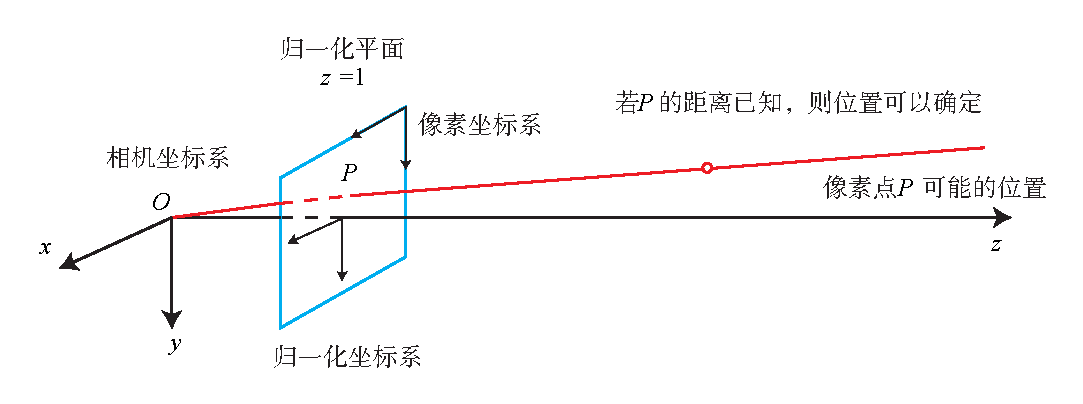
\includegraphics[width=1.0\textwidth]{cameraModel/pixelLocation.pdf}
    \caption{The possible location of a single pixel.}
    \label{fig:pixelLocation}
\end{figure}

There are many ways to measure the pixel distance (or depth). For example, the human eye can judge the object's distance according to the difference (or parallax) of the scene seen by the left and right eyes. The binocular camera principle is also the same. By simultaneously acquiring the left and right cameras' images and calculating the parallax/disparity between the images, each pixel's depth is estimated. In the following paragraph, we briefly describe the stereo camera's imaging principle (as shown in \autoref{fig:stereoCamera}~).

A binocular camera is generally composed of a left-eye camera and a right-eye camera. Of course, it can also be made up and down, but the mainstream binoculars we've seen are all left and right. Both the left and right cameras are regarded as simple pinhole cameras. They are synchronized and placed horizontally, meaning that both cameras' centers are on the same $x$ axis. The distance between the two centers is called \textit {baseline} (denoted as $b$), which is an important parameter.

\begin{figure}[!ht]
    \centering
    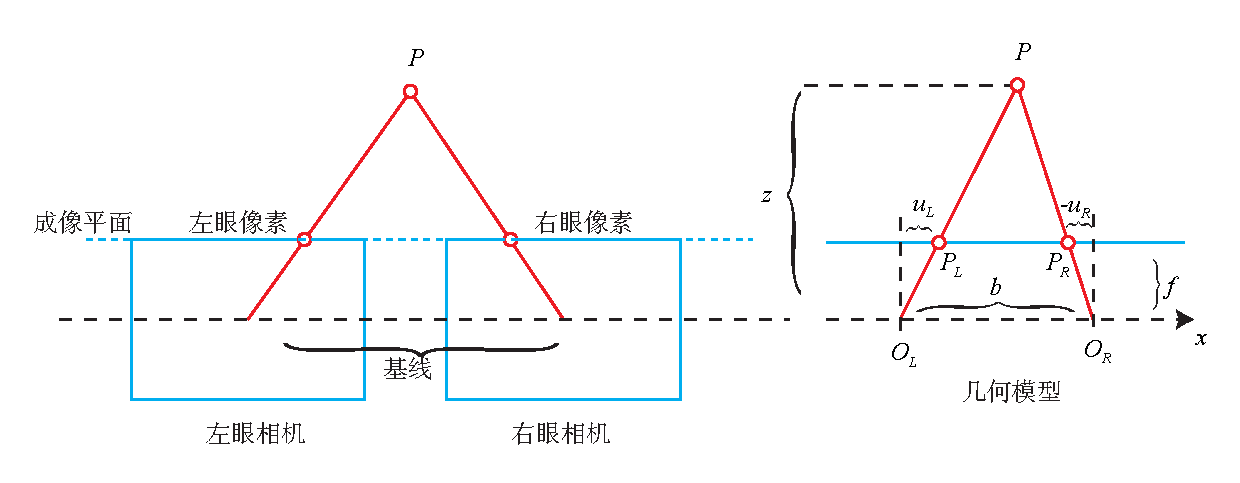
\includegraphics[width=1.0\textwidth]{cameraModel/stereoCamera.pdf}
    \caption{Geometry model of stereo cameras from upside down view. The $O_L, O_R$ are left and right optical centers. $f$ is the focal length, $u_L$ and $u_R$ are pixel coordinates of the same point along the $x$ axis. Note that $u_R$ should be a negative value in this figure, so the physical distance should be $-u_R$.}
    \label{fig:stereoCamera}
\end{figure}

Now consider a 3D point $P$, projected into the left-eye and the right-eye, written as $P_L, P_R$. Due to the presence of the camera baseline, these two imaging positions are different. Ideally, since the left and right cameras are only shifted on the $x$ axis, the image of $P$ also differs only on the $x$ axis (corresponding to the $u$ axis of the image). Take the left pixel coordinate as $u_L$ and the right coordinate as $u_R$. The geometric relationship is shown on the right of \autoref{fig:stereoCamera}. According to the similarity relationship between $ \triangle P P_L P_R$ and $\triangle P O_L O_R$, there are:

\begin{equation}
\frac{{z - f}}{z} = \frac{{b - {u_L} + {u_R}}}{b}.
\end{equation}

Rearrange it, and we have:
\begin{equation}
z = \frac{{fb}}{d}, \quad d \buildrel \Delta \over = {u_L} - {u_R},
\end{equation}
where $d$ is defined as the difference between the left and right figures' horizontal coordinates and is called disparity or parallax. Based on the parallax, we can estimate the distance between a pixel and the camera. Parallax is inversely proportional to distance: the larger the parallax is, the closer the distance is \footnote {Readers can simulate it with your own eyes.}. Simultaneously, since the parallax is at least one pixel, there is a theoretical maximum value for the binocular depth, which is determined by $fb$. To see the far-away things, we need a larger stereo camera; conversely, small binocular devices can only measure very close distances. By analogy, when the human eye looks at a very distant object (such as a very distant airplane), it is usually impossible to determine its distance accurately.

Although the depth's formula is simple, the real calculation of $d$ itself is more complicated. We need to know precisely where a pixel of the left-eye image appears in the right-eye image (that is, the corresponding relationship). This also belongs to the kind of task that is ``easy for humans but difficult for computers''. When we want to calculate each pixel's depth in an image, the calculation amount and accuracy will become a problem, and the parallax can be calculated only in the place where the image texture is rich. Due to the calculation amount, binocular depth estimation still needs GPU or FPGA to make the distance calculation run in real-time. This will be mentioned in lecture \ref{cpt:12}.

\subsection{RGB-D Cameras}
Compared to the binocular camera's way of calculating depth, the RGB-D camera's approach is more ``active'': it can actively measure each pixel's depth. The current RGB-D cameras can be divided into two categories according to their principle (see \autoref {fig:RGBDCamera} ~):

\begin{enumerate}
\item The first kind of RGB-D sensor uses structured infrared light to measure pixel distance. Many of the old RGB-D sensors are belong to this kind, for example, the Kinect 1st generation, Project Tango 1st generation, Intel RealSense, etc.
\item The second kind measures pixel distance using the \textit{time-of-flight (ToF)}. Examples are Kinect 2 and some existing ToF sensors in cellphones.
\end{enumerate}

\begin{figure}[!ht]
    \centering
    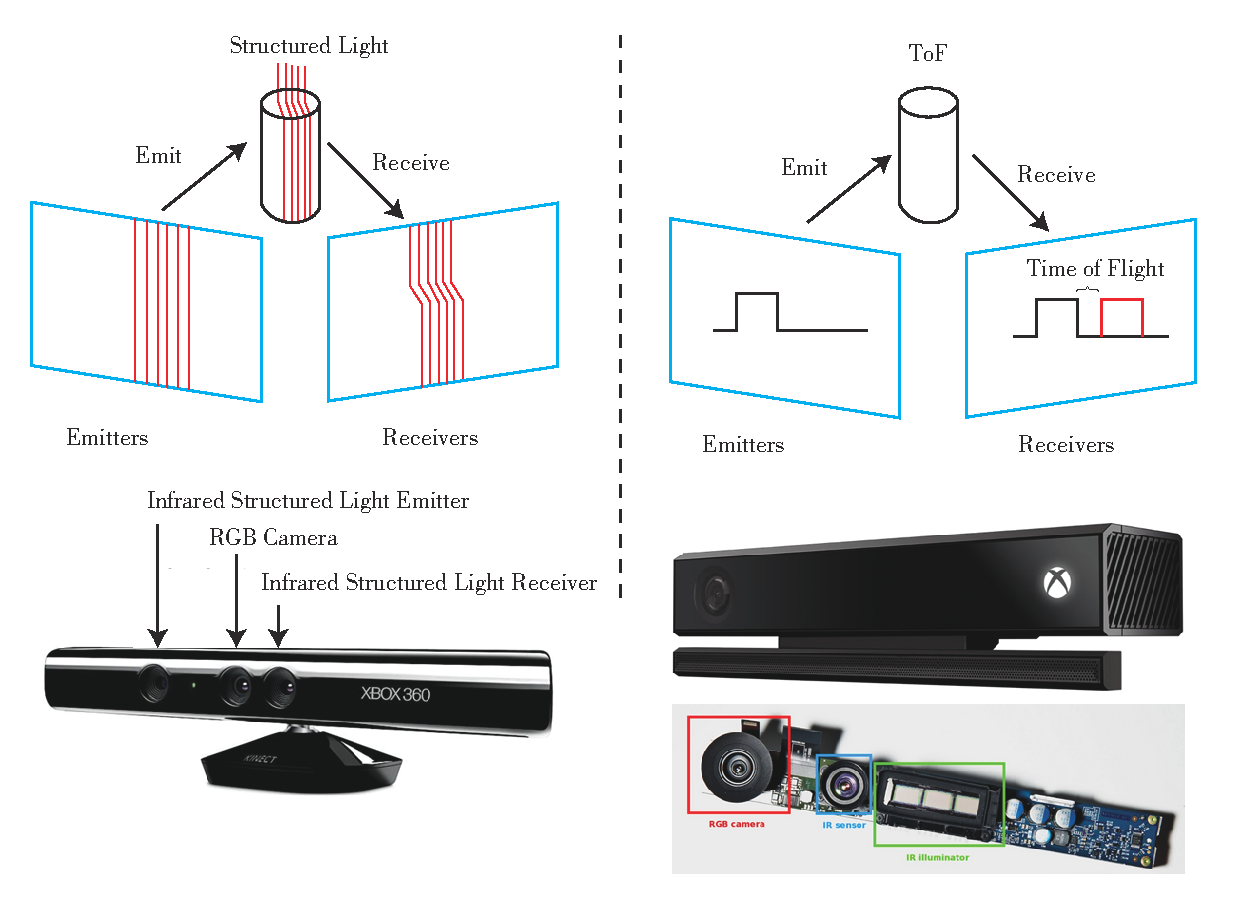
\includegraphics[width=1.0\textwidth]{cameraModel/rgbdCamera.pdf}
    \caption{RGB-D Cameras}
    \label{fig:RGBDCamera}
\end{figure}

Regardless of the type, the RGB-D camera needs to emit a light beam (usually infrared light) to the target object. In the structured light principle, the camera calculates the distance between the object and itself based on the returned structured light pattern. In the ToF principle, the camera emits a light pulse to the target and then determines the distance according to the beam's time of flight. The ToF principle is very similar to the laser sensor, except that the laser obtains the distance by scanning point by point (or line by line). The ToF camera can obtain the entire image's pixel depth, which is also the RGB-D camera's main advantage. So, if you take apart an RGB-D camera, you will usually find that there will be at least one transmitter and one receiver in addition to the ordinary camera.

After measuring the depth, the RGB-D camera usually completes the pairing between the depth and color map pixels according to each camera's position at the time of production. It outputs a pixel-to-pixel corresponding color image and depth image. We can read the color information and distance information at the same image position, calculate the 3D camera coordinates of the pixels, and generate a point cloud. RGB-D data can be processed either at the image level or the point cloud level. The second experiment of this lecture will demonstrate the point cloud construction of RGB-D cameras.

The RGB-D camera can measure the distance of each pixel in real-time. However, due to this measurement of transmitting and receiving, its range of use is limited. RGB-D cameras that use infrared light for depth measurement are susceptible to interference from infrared light emitted by daylight or other sensors, so they cannot be used outdoors. Without modulation, multiple RGB-D cameras can interfere with each other. These points' positions cannot be measured for transparent objects because they cannot receive reflected light. Also, RGB-D cameras have some disadvantages in terms of cost and power consumption.

\section{Images}
Cameras and lens convert the information in the three-dimensional world into a photo composed of pixels, which is then stored in the computer as a data source for subsequent processing. In mathematics, images can be described by a matrix; in computers, they occupy a continuous disk or memory space, which can be represented by a two-dimensional array. In this way, the program does not have to distinguish whether they are dealing with a numerical matrix or a meaningful image.

In this section, we will introduce some basic operations of computer image processing. In particular, we are going to introduce the basic steps of processing images with OpenCV and lay the foundation for subsequent chapters. Let's start with the simplest case, the grayscale image. Each pixel position $ (x, y) $ corresponds to a grayscale value of $ I $ in a grayscale image. Therefore, an image with the width of $ w $ and the height of $ h $ can be mathematically written as a function:
\[
(I) (x, y): \mathbb {R} ^ 2 \mapsto \mathbb {R},
\]
where $ (x, y) $ is the coordinate of the pixel. However, computers cannot express real numbers, so we need to quantify the subscripts and image readings within a certain range. For example, $ x, y $ are usually integers starting with 0 to $w-1, h-1$. In common grayscale images, an integer of $0 \textasciitilde 255$ (that is, an unsigned char in C++, 1 byte) is used to express the grayscale reading of the image. Then, a grayscale image with a width of 640 pixels and a height of 480 pixels can be expressed as:
\begin{lstlisting}[language=C++, caption=Use 2D array to express an image]
unsigned char image[480][640];
\end{lstlisting}

Why does the two-dimensional array here have the size of 480 $ \times $ 640? Because in the program, the first index of the 2D array is the row, and the second index is the column. In an image, the number of rows (or the $y$ axis) in the array corresponds to the height of the image, and the number of columns (or the $x$ axis) corresponds to the width of the image.
\begin{figure}[!t]
    \centering
    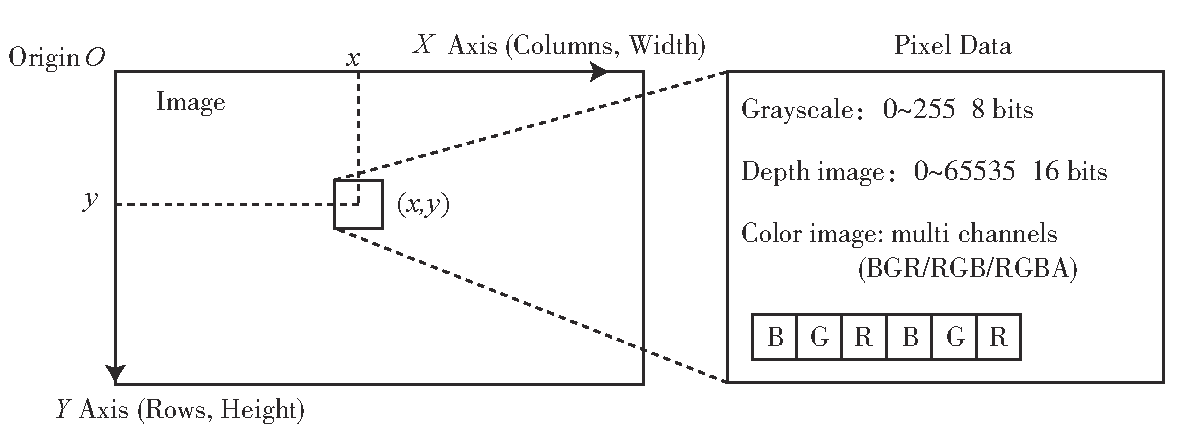
\includegraphics[width=0.84\textwidth]{cameraModel/image.pdf}
    \caption{Pixels in an image.}
    \label{fig:imagesInComputer}
\end{figure}

Let's examine the content of this image. Images are naturally made up of pixels. When accessing a certain pixel, you need to specify its coordinates, as shown in \autoref{fig:imagesInComputer}~. The left side of the figure shows how the traditional pixel coordinate system is defined. The origin is in the upper left corner of the image, the $X$ axis is from left to right, and the $Y$ is top-down. If it has a third axis, the $ Z $ axis, then according to the right-hand rule, the $ Z $ axis should be from outside to inside (or front in 3D space). This definition is consistent with the camera coordinate system. The width or number of columns of an image corresponds to the $ X $ axis; the number of rows or the height of an image corresponds to its $ Y $ axis.

According to this definition, if we discuss a pixel located at $x,y$, then the code of accessing its memory in the computer should be:
\begin{lstlisting}[language = C++, caption = Accessing image pixels]
unsigned char pixel = image[y][x];
\end{lstlisting}

It corresponds to the reading of the gray value $ I(x,y) $. Please note the order of $ x $ and $ y $ here. Although we tirelessly discuss the problem of coordinate systems, errors like this index sequence will still be one of the most common errors encountered by novices during debugging. If you accidentally change the coordinates of $ x, y $ when writing a program, the compiler cannot provide any useful information at compile-time. All you can see is a segment fault in runtime.

A pixel's grayscale can be recorded as an 8-bit unsigned integer, which is a value of $0\textasciitilde 255$. If we have more information to record, one byte is probably not enough. For example, in the depth map of an RGB-D camera, each pixel's distance is recorded. This distance is usually measured in millimeters, and the range of RGB-D cameras is usually around a dozen meters, exceeding 255. At this time, people will use 16-bit integers (unsigned short in C++) to record the depth map information, that is, the value at $0 \textasciitilde 65535$. When converted to meters, it can represent up to 65 meters, which is enough for RGB-D cameras.

The representation of a color image requires the concept of a channel. In computers, we use three colors: red, green, and blue to express any color. Therefore, for each pixel, three R, G, and B values are recorded, and each value is called a channel. For example, the most common color image has three channels, represented by an 8-bit integer. Under this rule, one pixel occupies a 24-bit space.

The number and order of channels can be freely defined. In OpenCV color images, the default order of channels is B, G, R, which means when we get a 24-bit pixel, the first 8 bits represent the blue value, the middle 8 bits represent the green, and the last 8 bits represent the red. Similarly, the order of R, G, and B can also be used to describe a color image. If you want to express the image's transparency, use R, G, B, A four channels.

\section{Practice: Images in Computer Vision}
\subsection{Basic Usage of OpenCV}
The following is a demo program to help you understand how to access the image in OpenCV and how to visit its pixels.

\subsubsection{Install OpenCV}
OpenCV \footnote {Official homepage: \url{http://opencv.org}. } provides many open-source image algorithms and is a very widely used image processing algorithm library in computer vision. This book also uses OpenCV for basic image processing. Before using, readers must install it from the pre-compiled library or from source code. Under Ubuntu, there are two options: \textit{install from source code} or \textit {only install binary library files}:

\begin{enumerate}
\item Install from source means to download all OpenCV source code from the OpenCV website, compile and install on the machine for usage. The advantage is that you can freely choose which version to install, and the source code is accessible, but it takes some compilation time.
\item Or, we can only install the binary library file, which means it was pre-compiled by the Ubuntu community, so there is no need to recompile it.
\end{enumerate}

If we use a newer version of OpenCV than that in the apt source, we must install it from the source code. First, you can adjust some compilation options to match the programming environment (for example, to disable some unused modules or turn on the GPU acceleration, etc.). OpenCV currently maintains two major versions, divided into OpenCV 2.4 series and OpenCV 3 series \footnote{In 2020, we can also use version 4.0 or higher.}. This book uses the OpenCV \textit {3} or higher.

Because the OpenCV project is relatively large, it will not be placed under 3rdparty in this book. Readers can download it from ~ \url{http://opencv.org/downloads.html}~ and select the Linux version. You will get a compressed package like opencv-3.1.0.zip. Unzip it to any directory, we can found that OpenCV is also a CMake project.

Before compiling, first, install the dependencies of OpenCV:
\begin{lstlisting}[language=sh, caption=Terminal input:]
sudo apt-get install build-essential libgtk2.0-dev libvtk5-dev libjpeg-dev libtiff4-dev libjasper-dev libopenexr-dev libtbb-dev
\end{lstlisting}

In fact, OpenCV has many dependencies, and the lack of certain dependency items will affect some of its functions (but we will not use all the functions). OpenCV will check whether the dependencies will be installed during CMake and adjust its own configurations. If you have a GPU on your computer and the relevant dependencies are installed, OpenCV will also enable GPU acceleration. But for this book, the above dependencies are sufficient.

Subsequent compilation and installation are the same as ordinary CMake projects. After make, please call ``sudo make install'' to install OpenCV on your machine (instead of just compiling it). Depending on the machine configuration, this compilation process may take from 20 minutes to an hour. If your CPU is powerful, you can use commands like ``make -j4'' to call multiple threads to compile (the parameter after -j is the number of threads used). After installation, OpenCV is stored in the /usr/local directory by default. You can look for OpenCV header files and library files' installation location to see where they are. Besides, if you have installed the OpenCV 2 series before, it is recommended that you install OpenCV 3 elsewhere (think about how this should be done).

\subsection{Basic OpenCV Images Operations}
Now let's go through the basic image operations in OpenCV from a simple example.

\begin{lstlisting}[language=C++,caption=slambook/ch5/imageBasics/imageBasics.cpp]
#include <iostream>
#include <chrono>

using namespace std;

#include <opencv2/core/core.hpp>
#include <opencv2/highgui/highgui.hpp>

int main(int argc, char **argv) {
    // Read the image in argv[1]
    cv::Mat image;
    image = cv::imread(argv[1]); // call cv::imread to read the image from file
    
    // check the data is correctly loaded
    if (image.data == nullptr) { // maybe the file does not exist
        cerr << "file" << argv[1] << " not exist." << endl;
        return 0;
    }
    
    // print some basic information
    cout << "Image cols: " << image.cols << ", rows: " << image.rows 
	    << ", channels: " << image.channels() << endl;
    cv::imshow("image", image);      // use cv::imshow to show the image
    cv::waitKey(0);                  // display and wait for a keyboard input
    
    // check image type
    if (image.type() != CV_8UC1 && image.type() != CV_8UC3) {
        // we need grayscale image or RGB image
        cout << "image type incorrect." << endl;
        return 0;
    }
    
    // check hte pixels
    chrono::steady_clock::time_point t1 = chrono::steady_clock::now();
    for (size_t y = 0; y < image.rows; y++) {
        // use cv::Mat::ptr to get the pointer of each row
        unsigned char *row_ptr = image.ptr<unsigned char>(y);  // row_ptr is the pointer to y-th row
        for (size_t x = 0; x < image.cols; x++) {
            // read the pixel on (x,y), x=column, y=row
            unsigned char *data_ptr = &row_ptr[x * image.channels()]; // data_ptr is the pointer to (x,y)
            // visit the pixel in each channel
            for (int c = 0; c != image.channels(); c++) {
                unsigned char data = data_ptr[c]; // data should be pixel of I(x,y) in c-th channel
            }
        }
    }
    chrono::steady_clock::time_point t2 = chrono::steady_clock::now();
    chrono::duration<double> time_used = chrono::duration_cast < chrono::duration < double >> (t2 - t1);
    cout << "time used: " << time_used.count() << " seconds." << endl;
    
    // copying cv::Mat
    // operator = will not copy the image data, but only the reference
    cv::Mat image_another = image;
    // changing image_another will also change image 
    image_another(cv::Rect(0, 0, 100, 100)).setTo(0); // set top-left 100*100 block to zero
    cv::imshow("image", image);
    cv::waitKey(0);
    
    // use cv::Mat::clone to actually clone the data
    cv::Mat image_clone = image.clone();
    image_clone(cv::Rect(0, 0, 100, 100)).setTo(255);
    cv::imshow("image", image);
    cv::imshow("image_clone", image_clone);
    cv::waitKey(0);
    
    // We are not going to copy the OpenCV's documentation here
    // please take a look at it for other image operations like clipping, rotating and scaling.
    
    cv::destroyAllWindows();
    return 0;
}
\end{lstlisting}

In this example, we demonstrated the following operations: image reading, displaying, pixel vising, copying, assignment, etc. When compiling the program, you need to add the OpenCV header file in your ``CMakeLists.txt'', and then link the program to the OpenCV's library. At the same time, due to the use of C++ 11 standards (such as the nullptr and chrono), you also need to set up the c++ standard in the compiler flag:

\begin{lstlisting}[language=Python,caption=slambook/ch5/imageBasics/CMakeLists.txt]
# use c++11 standard
set( CMAKE_CXX_FLAGS "-std=c++11" )

# find OpenCV
find_package( OpenCV REQUIRED )
# include its headers
include_directories( ${OpenCV_INCLUDE_DIRS} )

add_executable( imageBasics imageBasics.cpp )

# link the exe to opencv's libs
target_link_libraries( imageBasics ${OpenCV_LIBS} )
\end{lstlisting}

Let's give some notes for the code:
\begin{enumerate}
\item The program reads the image position from argv[1], the first parameter on the command line. We prepared an image (ubuntu.png, an Ubuntu wallpaper, hope you like it) for readers to test. Therefore, after compilation, use the following command to call this program:
\begin{lstlisting}[language=sh, caption=Terminal input:]
./build/imageBasics ubuntu.png
\end{lstlisting}
If you call this program in the IDE, be sure to give it parameters at the same time. This can be configured in the launch configuration dialog if you are using Clion.
\item In line 10 \textasciitilde to 18, we use the cv::imread function to read the image. And then, we display the image and its basic information.
\item In line 35 \textasciitilde 46, we iterate over all pixels in the image and calculates the time spent in the entire loop. Please note that the pixel visiting method is not unique, and the method given by the example is not the most efficient way. OpenCV provides an iterator of cv::Mat. You can traverse the pixels of the image through the iterator. Or, cv::Mat::data provides a raw pointer to the beginning of the image data. You can also directly calculate the offset through this pointer, and then get the memory location of the pixel. The method used in the example is to facilitate the reader to understand the structure of the image.

\item OpenCV provides many functions for manipulating images. We will not list them one by one. Otherwise, this book will become an OpenCV operation manual. The example shows the most common things like image reading and displaying and the deep copy function in cv::Mat. During the programming process, readers will also encounter operations such as image rotation and interpolation. At this time, you should refer to the corresponding documentation of the function to understand their principles and usage.
\end{enumerate}

It should be noted that OpenCV is not the only image library. It is just one of the more widely used ones. However, most image libraries have similar image operations. We hope that readers can understand the representation of images in other libraries after using OpenCV to quickly adjust to any other libraries. Since cv::Mat is also a matrix class, we can also use it to store matrix data such as rotation matrix and do some linear algebra operations. But it is generally believed that \textit{Eigen} is more efficient for use with fixed-size matrices.

\subsection{Image Undistortion}
We've introduced the rad-tan distortion model in the previous section, now let write an example to show the implementation. OpenCV has provided the cv::Undistort function for us, but we will also give a hand-written undistortion function to show the principles.

\begin{lstlisting}[language=C++,caption=slambook/ch5/imageBasics/undistortImage.cpp]
#include <opencv2/opencv.hpp>
#include <string>
using namespace std;
string image_file = "./distorted.png";   // the distorted image 

int main(int argc, char **argv) {
    // In thie program we implement the undistortion by ourselves rather than using opencv
    // rad-tan model params
    double k1 = -0.28340811, k2 = 0.07395907, p1 = 0.00019359, p2 = 1.76187114e-05;
    // intrinsics
    double fx = 458.654, fy = 457.296, cx = 367.215, cy = 248.375;
    
    cv::Mat image = cv::imread(image_file, 0);   // the image type is CV_8UC1
    int rows = image.rows, cols = image.cols;
    cv::Mat image_undistort = cv::Mat(rows, cols, CV_8UC1);   // the undistorted image
    
    // computate the pixels in the undistorted one
    for (int v = 0; v < rows; v++) {
        for (int u = 0; u < cols; u++) {
            // note we are computing the pixel of (u,v) in the undistorted image
            // according to the rad-tan model, compute the coordinates in the distorted image
            double x = (u - cx) / fx, y = (v - cy) / fy;
            double r = sqrt(x * x + y * y);
            double x_distorted = x * (1 + k1 * r * r + k2 * r * r * r * r) + 2 * p1 * x * y + p2 * (r * r + 2 * x * x);
            double y_distorted = y * (1 + k1 * r * r + k2 * r * r * r * r) + p1 * (r * r + 2 * y * y) + 2 * p2 * x * y;
            double u_distorted = fx * x_distorted + cx;
            double v_distorted = fy * y_distorted + cy;
            
            // check if the pixel is in the image boarder
            if (u_distorted >= 0 && v_distorted >= 0 && u_distorted < cols && v_distorted < rows) {
                image_undistort.at<uchar>(v, u) = image.at<uchar>((int) v_distorted, (int) u_distorted);
            } else {
                image_undistort.at<uchar>(v, u) = 0;
            }
        }
    }
    
    // show the undistorted image
    cv::imshow("distorted", image);
    cv::imshow("undistorted", image_undistort);
    cv::waitKey();
    return 0;
}
\end{lstlisting}

Please check the difference between the two images by yourself.

\section{Practice: 3D Vision}
\subsection{Stereo Vision}
We have introduced the imaging principle of stereo vision. Now we start from the left and right images, calculate the disparity map corresponding to the left eye, and then calculate each pixel's coordinates in the camera coordinate system, which will form a \textit{point cloud}. We have prepared left and right images for the readers, as shown in \autoref {fig:stereoExample}. The following code demonstrates the calculation of disparity map and point cloud:

\begin{lstlisting}[language=C++,caption=slambook/ch5/stereoVision/stereoVision.cpp (Part)]
int main(int argc, char **argv) {
    // intrinsics
    double fx = 718.856, fy = 718.856, cx = 607.1928, cy = 185.2157;
    // baseline
    double b = 0.573;
    
    cv::Mat left = cv::imread(left_file, 0);
    cv::Mat right = cv::imread(right_file, 0);
    cv::Ptr<cv::StereoSGBM> sgbm = cv::StereoSGBM::create(
        0, 96, 9, 8 * 9 * 9, 32 * 9 * 9, 1, 63, 10, 100, 32);    // SGBM is senstive to parameters
    cv::Mat disparity_sgbm, disparity;
    sgbm->compute(left, right, disparity_sgbm);
    disparity_sgbm.convertTo(disparity, CV_32F, 1.0 / 16.0f);
    
    // compute the point cloud
    vector<Vector4d, Eigen::aligned_allocator<Vector4d>> pointcloud;
    
    // change v++ and u++ to v+=2, u+=2 if your machine is slow to get a sparser cloud
    for (int v = 0; v < left.rows; v++)
    for (int u = 0; u < left.cols; u++) {
        if (disparity.at<float>(v, u) <= 10.0 || disparity.at<float>(v, u) >= 96.0) continue;
        
        Vector4d point(0, 0, 0, left.at<uchar>(v, u) / 255.0); // the first three dimensions are xyz, the 4-th is the color
        
        // compute the depth from disparity
        double x = (u - cx) / fx;
        double y = (v - cy) / fy;
        double depth = fx * b / (disparity.at<float>(v, u));
        point[0] = x * depth;
        point[1] = y * depth;
        point[2] = depth;
        
        pointcloud.push_back(point);
    }
    
    cv::imshow("disparity", disparity / 96.0);
    cv::waitKey(0);
    
    // show the point cloud in pangolin
    showPointCloud(pointcloud);
    return 0;
}
\end{lstlisting}

\begin{figure}[!t]
    \centering
    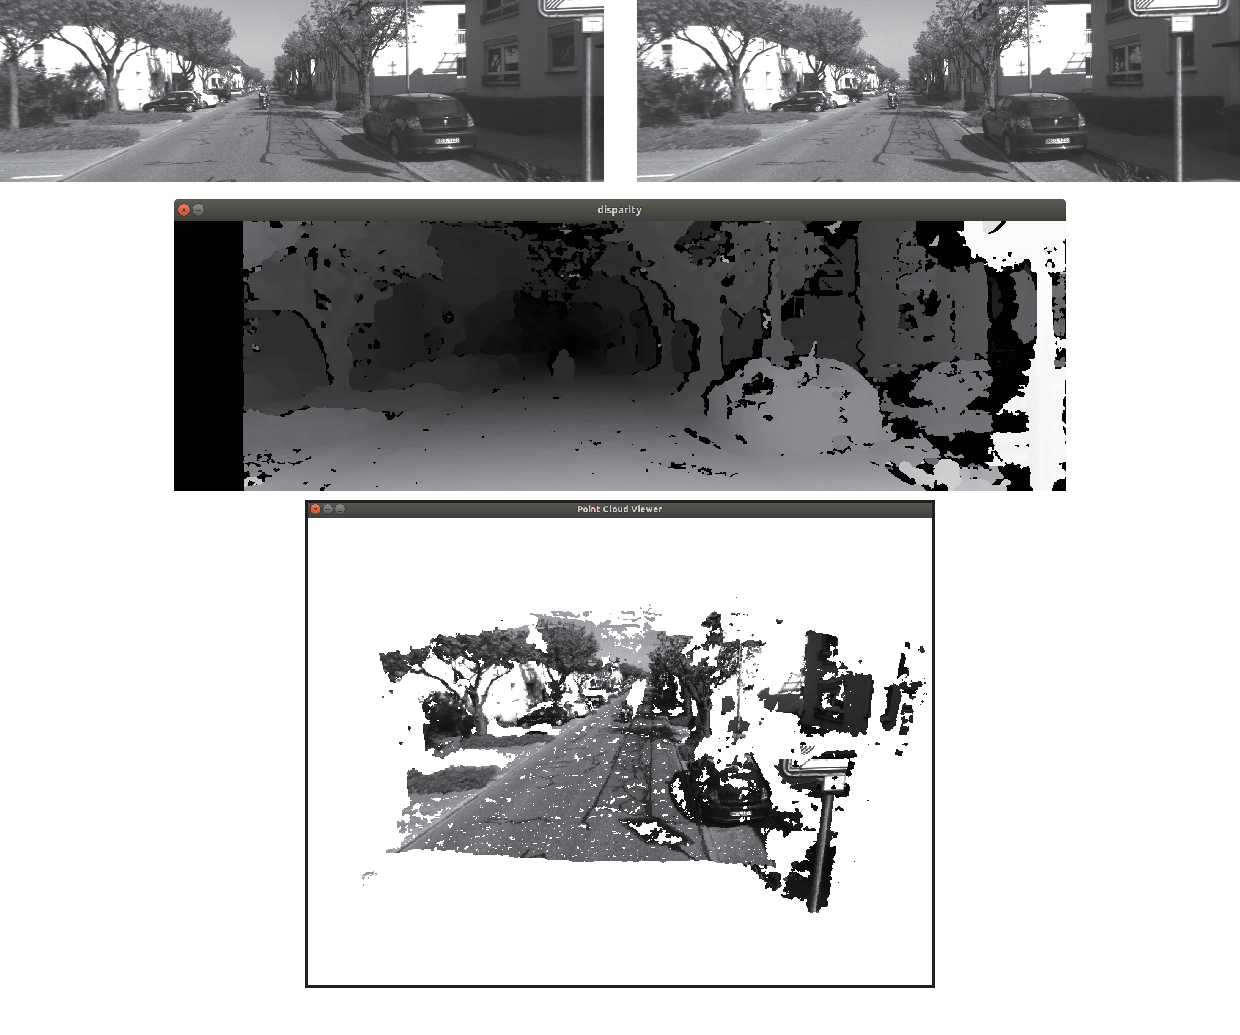
\includegraphics[width=0.9\textwidth]{cameraModel/stereoExample.pdf}
    \caption{Stereo image example. Top-left: left image, top-right: right image, mid: SGBM disparity map, bottom: point cloud. Note that since some of the pixels in the left image is not seen in the right one, so the disparity map will have some empty values.}
    \label{fig:stereoExample}
\end{figure}

In this example, we call the SGBM (Semi-global Batch Matching) {\cite{Hirschmuller2008}} algorithm implemented by OpenCV to calculate the disparity of the left and right images and then transform it into the 3D space of the camera through the geometric model of the binocular camera. We use a classic parameter configuration from the internet, and we mainly adjust the maximum and minimum disparity. The disparity data combined with the camera's internal parameters and baseline can determine each point's position in three-dimensional space. We omit the code related to displaying the point cloud to save some space.

This book is not going to introduce the disparity calculation algorithm of the binocular camera. Interested readers can read the relevant references {\cite{Scharstein2002, Seitz2006}}. In addition to the binocular algorithm implemented by OpenCV, there are many other libraries focused on achieving efficient parallax calculations. It is still an active and complex subject today.

\subsection{RGB-D Vision}
\label{sec:join-point-cloud}
Finally, we demonstrate an example of RGB-D vision. The convenience of RGB-D cameras is that they can obtain pixel depth information through physical methods. If the camera's intrinsic and extrinsic are known, we can calculate any pixel position in the world coordinate system, thereby creating a point cloud map. Now let's demonstrate how to do it.

We have prepared 5 pairs of images located in the slambook2/ch5/rgbd folder. There are 5 RGB images from 1.png to 5.png under the color/ directory and 5 corresponding depth images under the depth/. At the same time, the ``pose.txt'' file gives the camera poses of the 5 images (in the form of $ \mathbf{T}_\mathrm{wc} $). The format of the pose record is the same as before, with the translation vector plus a rotation quaternion:
\[
[x, y, z, q_x, q_y, q_z, q_w],
\]
where $q_w$ is the real part of the quaternion. For example, the parameters of the first pair of image are:
\[
[-0.228993, 0.00645704, 0.0287837, -0.0004327, -0.113131, -0.0326832, 0.993042].
\]

Below we write a program to accomplish two things: (1) We calculate the point cloud corresponding to each pair of RGB-D images based on internal parameters; (2) According to the camera pose of each image, we put the points to a global cloud by the camera poses.

\begin{lstlisting}[language=C++,caption=slambook/ch5/rgbd/jointMap.cpp (Part)]
int main(int argc, char **argv) {
    vector<cv::Mat> colorImgs, depthImgs;
    TrajectoryType poses;         // camera poses
    
    ifstream fin("./pose.txt");
    if (!fin) {
        cerr << "Please run the program in the directory that has pose.txt" << endl;
        return 1;
    }
    
    for (int i = 0; i < 5; i++) {
        boost::format fmt("./%s/%d.%s"); // the image format
        colorImgs.push_back(cv::imread((fmt % "color" % (i + 1) % "png").str()));
        depthImgs.push_back(cv::imread((fmt % "depth" % (i + 1) % "pgm").str(), -1)); // use -1 flag to load the depth image
        
        double data[7] = {0};
        for (auto &d:data) fin >> d;
        Sophus::SE3d pose(Eigen::Quaterniond(data[6], data[3], data[4], data[5]),
        Eigen::Vector3d(data[0], data[1], data[2]));
        poses.push_back(pose);
    }
    
    // compute the point cloud using camera intrinsics
    double cx = 325.5;
    double cy = 253.5;
    double fx = 518.0;
    double fy = 519.0;
    double depthScale = 1000.0;
    vector<Vector6d, Eigen::aligned_allocator<Vector6d>> pointcloud;
    pointcloud.reserve(1000000);
    
    for (int i = 0; i < 5; i++) {
        cout << "Converting RGBD images " << i + 1 << endl;
        cv::Mat color = colorImgs[i];
        cv::Mat depth = depthImgs[i];
        Sophus::SE3d T = poses[i];
        for (int v = 0; v < color.rows; v++)
        for (int u = 0; u < color.cols; u++) {
            unsigned int d = depth.ptr<unsigned short>(v)[u]; // depth value is 16-bit
            if (d == 0) continue; // 0 means no valid value
            Eigen::Vector3d point;
            point[2] = double(d) / depthScale;
            point[0] = (u - cx) * point[2] / fx;
            point[1] = (v - cy) * point[2] / fy;
            Eigen::Vector3d pointWorld = T * point;
            
            Vector6d p;
            p.head<3>() = pointWorld;
            p[5] = color.data[v * color.step + u * color.channels()];   // blue
            p[4] = color.data[v * color.step + u * color.channels() + 1]; // green
            p[3] = color.data[v * color.step + u * color.channels() + 2]; // red
            pointcloud.push_back(p);
        }
    }
    
    cout << "global point cloud has " << pointcloud.size() << " points." << endl;
    showPointCloud(pointcloud);
    return 0;
}
\end{lstlisting}

We can see the point cloud in \textit{Pangolin} after building it (see \autoref{fig:pointcloudmapping}).

\begin{figure}[!t]
    \centering
    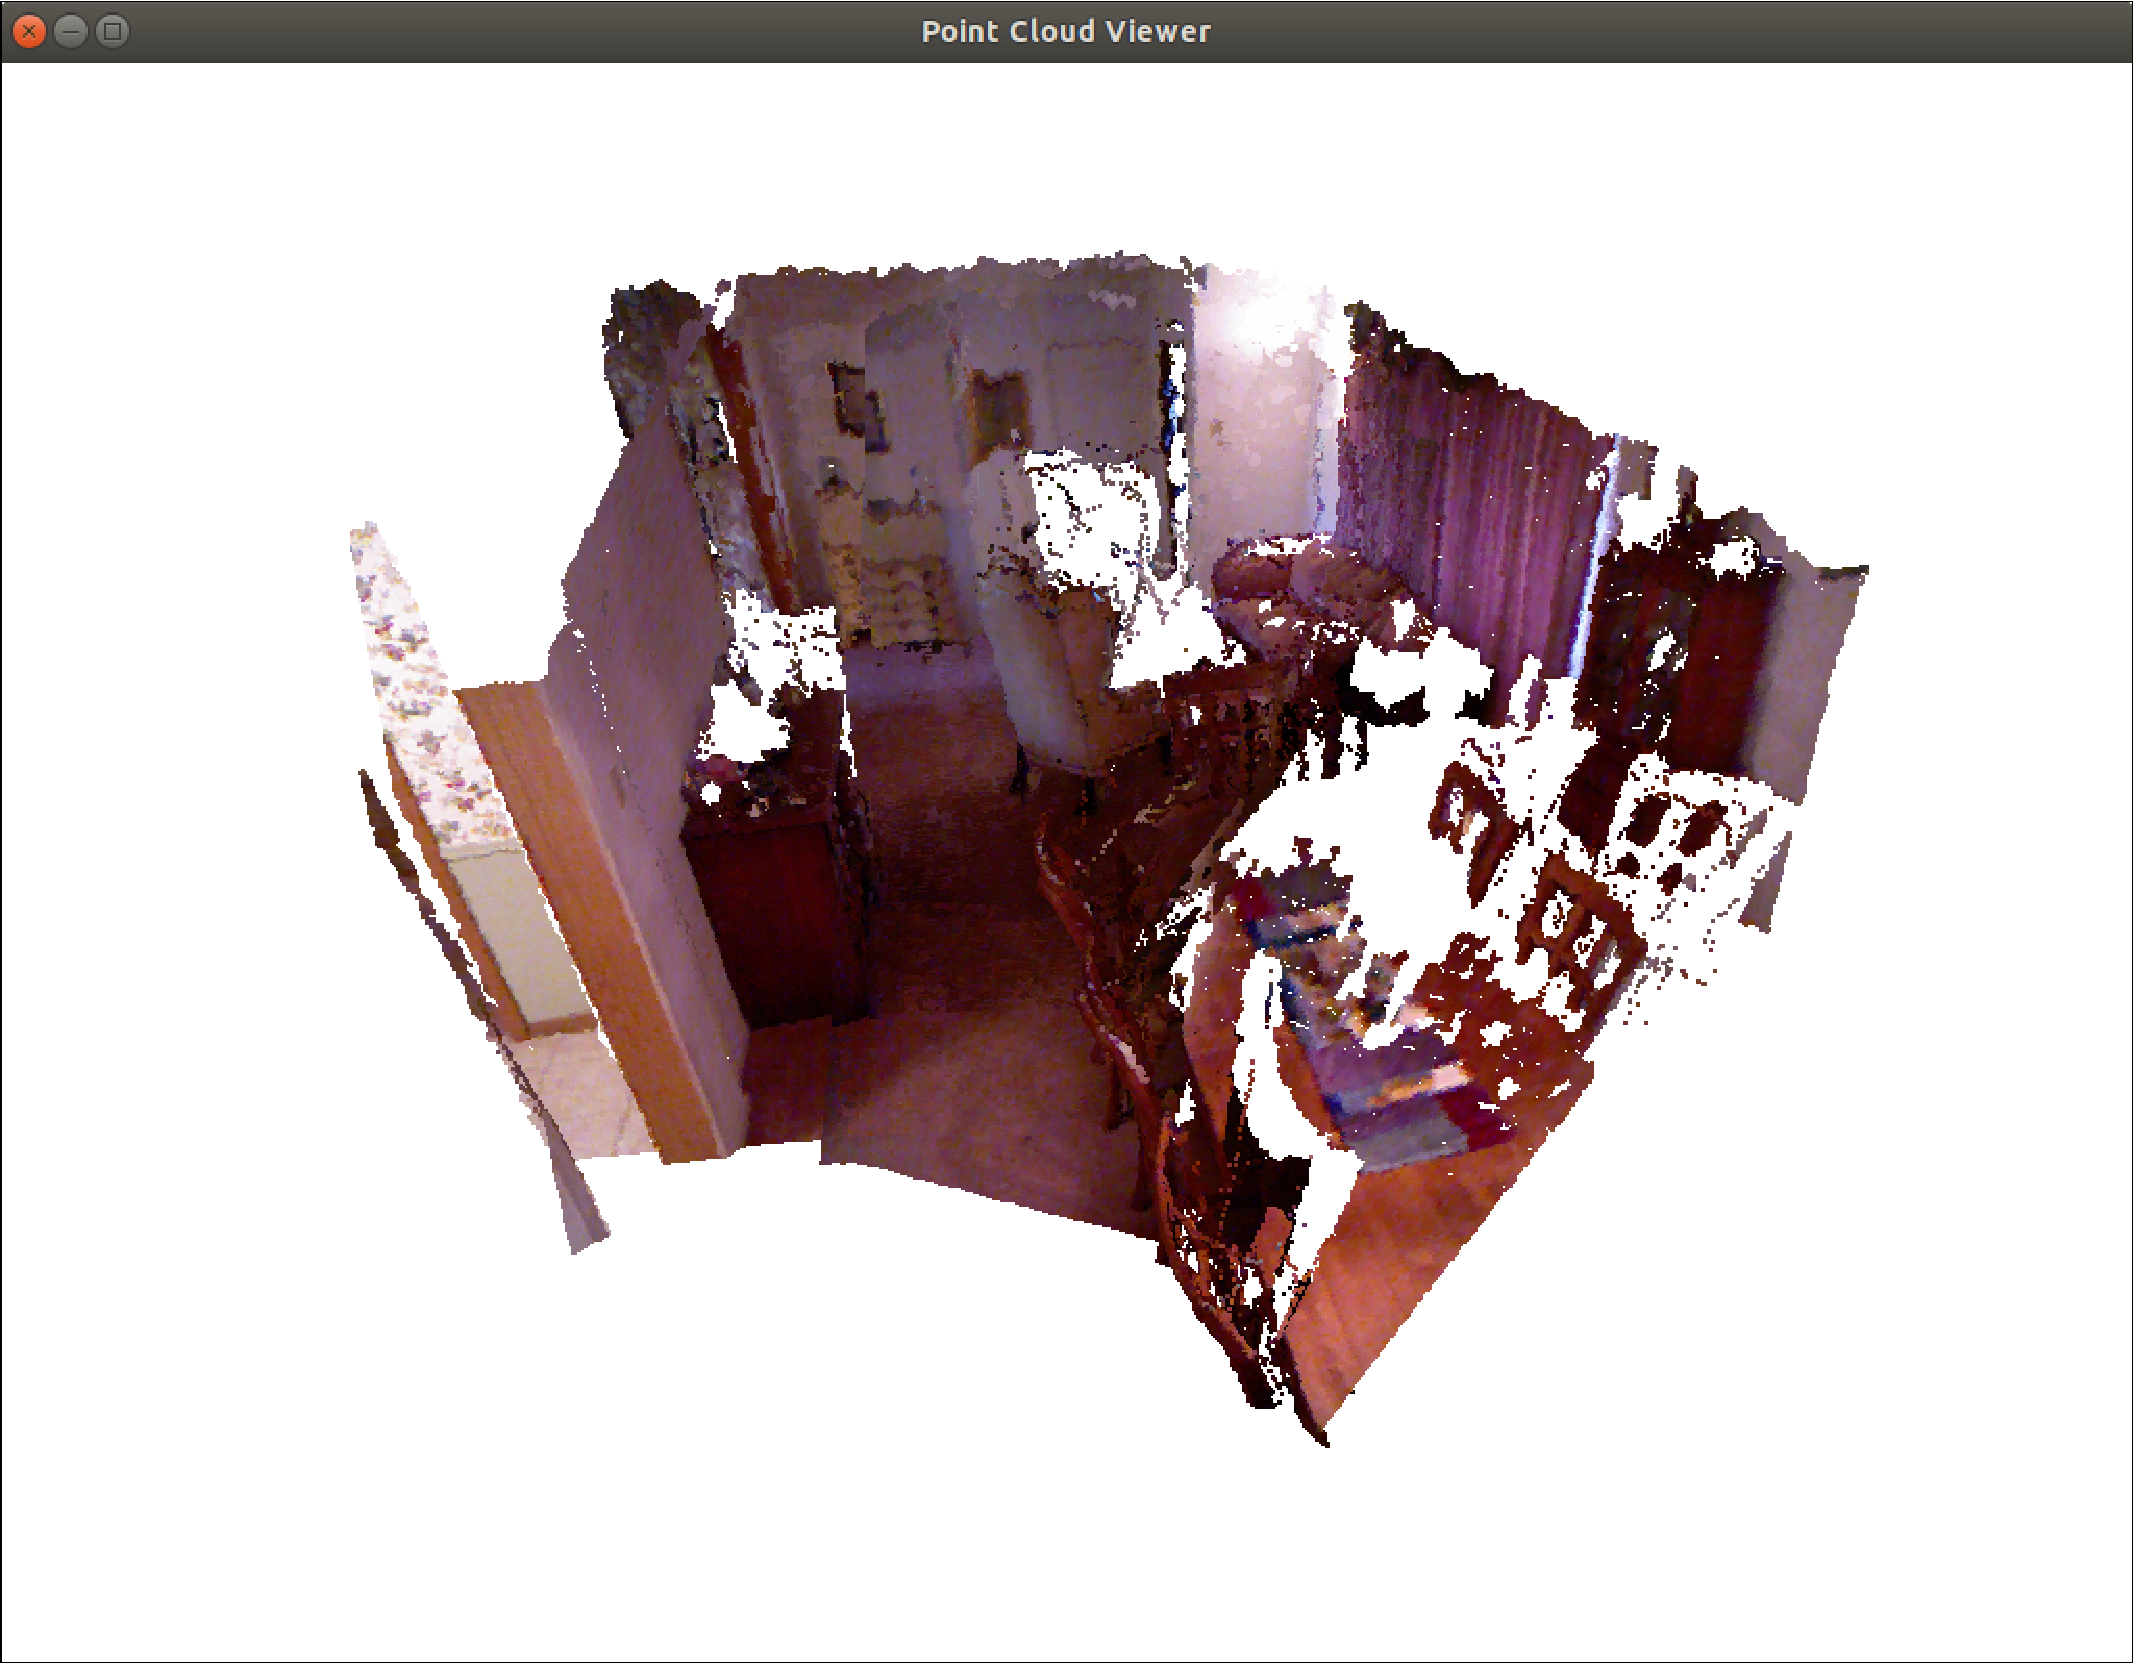
\includegraphics[width=1.0\textwidth]{cameraModel/pointcloud.pdf}
    \caption{The global point cloud from 5 RGBD image pairs.}
    \label{fig:pointcloudmapping}
\end{figure}

We demonstrated some common monocular, binocular, and rgbd camera algorithms in computer vision through these examples. We hope readers can understand the meaning of the intrinsics, extrinsics, and distortion model through them.

\section * {Exercise}
\begin{enumerate}
\item[\optional] Find a camera (use the camera of your mobile phone or laptop if you don't have one) and calibrate its internal parameters. You may use a calibration board or print out a checkerboard for calibration.
\item Describes the physical meaning of the camera's intrinsics. If the resolution of a camera is doubled and the rest is unchanged, how does its intrinsic change?
\item Search for the calibration method of special cameras (fisheye or panoramic cameras). Where are the differences between them and the pinhole models? 
\item Investigate the similarities and differences between a global shutter camera and a rolling shutter camera. What are their advantages and disadvantages in SLAM?
\item How are RGB-D cameras calibrated? Taking Kinect as an example, what parameters need to be calibrated? (Refer to \url{https://github.com/code-iai/iai_kinect2}.)
\item In addition to the way of traversing the image demonstrated by the sample program, what other methods can you give to traverse the image?
\item[\optional] Read the official OpenCV tutorial to learn its basic usage.
\end{enumerate}


% ch6 非线性优化
% !Mode:: "TeX:UTF-8"
\chapter{Nonlinear Optimization}
\label{cpt:6}
\begin{mdframed}  
	\textbf{Goal of This Chapter}
	\begin{enumerate}[labelindent=0em,leftmargin=1.5em]
		\item Understand how to form the batch state estimation problem into a least square and how to solve the least square problem.
		\item Understand the Gauss-Newton and Levenburg-Marquadt method and implement them.
		\item Learn how to use the Google Ceres and g2o library to solve a least square problem.
	\end{enumerate}
\end{mdframed} 

In the previous lectures, we introduced the motion and observation equations of the classic SLAM model. Now we know that the pose in the equation can be described by the transformation matrix and then optimized by Lie algebra. The observation equation is given by the camera imaging model, in which the internal parameter is fixed with the camera, and the external parameter is the pose of the camera. So, we have figured out the concrete expression of the classic visual SLAM model.

However, due to the presence of noise, the equations of motion and observation can not be exactly met. Although the camera can fit the pinhole model very well, unfortunately, the data we get is usually affected by various unknown noises. Even if we have a high-precision camera and controller, the motion and observations equations can only be approximated. Therefore, instead of assuming that the data must conform to the equation, it is better to estimate the state from the noisy data accurately.

Solving the state estimation problem requires a certain degree of optimization background knowledge. This section will introduce the basic unconstrained nonlinear optimization method and introduce optimization libraries g2o and Ceres.

\newpage
\includepdf{resources/other/ch6.pdf}

\newpage
\section{State Estimation}
\subsection{From Batch State Estimation to Least Square}
According to the previous sections, the SLAM process can be described by a discrete time motion and observation equations like~\eqref{eq:slamproblem}:
\begin{equation}
\left\{ \begin{array}{l}
{\bm{x}_k} = \mathbf{f}\left( {{\bm{x}_{k - 1}},{\bm{u}_k}} \right) + \bm{w}_k\\
{\bm{z}_{k,j}} = \mathbf{h}\left( {{ \bm{y}_j},{ \bm{x}_k}}  \right)+ \bm{v}_{k,j}
\end{array} \right. .
\end{equation}

Through the knowledge in Lecture 4, we learned that $ \bm {x} _k $ is the pose of the camera, which can be described by $ \mathrm {SE} (3) $. As for the observation equation, we have already explained in Lecture 5, the pinhole camera model. In order to give readers a deeper impression of them, we may wish to discuss their specific parameterized form. First, the pose variable $\bm {x} _k $ can be expressed by $\bm {T} _k \in \mathrm {SE} (3) $. Second, the motion is related to the specific form of the input, but there is no particularity in visual SLAM (should be same as the case of ordinary robots and vehicles), we will not talk about it for the time being. The observation equation is given by the pinhole model. Assuming an observation of the road sign $ \bm {y} _j $ at $ \bm {x} _k $, corresponding to the pixel position on the image $ \bm {z} _ {k, j} $, then, observe The equation can be expressed as:
\begin{equation}
s \bm{z}_{k,j}= \bm{K} (\bm{R}_k {\bm{y}_j}+\bm{t}_k),
\end{equation}
where $ \bm {K} $ is the intrinsic matrix of the camera, and $s$ is the distance of pixels, which is also the third element of $ (\bm {R} _k {\bm {y} _j} + \bm {t} _k) $. If we use  transformation matrix $ \bm {T} _k $ to describe the pose, then the points $ \bm {y} _j $ must be described in homogeneous coordinates, and then converted to non-homogeneous coordinates afterwards. If you are not familiar with this process, please go back to the previous lectures.

Now, consider what happens when the data is affected by noise. In the motion and observation equations, we \textbf {usually} assume that the two noise terms $ \bm {w} _k, \bm {v} _ {k, j} $ satisfy a Gaussian distribution with zero mean, like this:
\begin{equation}
{\bm{w}_k} \sim \mathcal{N}\left( {\bm{0},{\bm{R}_k}} \right),{\bm{v}_k} \sim \mathcal{N}\left( {\bm{0},{{{\bm{Q}}}_{k,j}}} \right),
\end{equation}
where $ \mathcal {N} $ means Gaussian distribution, $ \bm{0} $ means zero mean, and $ \bm {R} _k, \bm {Q} _ {k, j} $ is the covariance matrix. Under the influence of these noises, we hope to infer the pose $ \bm {x} $ and the map $ \bm {y} $ from the noisy data $ \bm {z} $ and $ \bm {u} $ (and their probability density distribution), which constitutes a state estimation problem.

There are two ways to deal with this state estimation problem. Since these data come gradually over time in the SLAM process, we should intuitively hold an estimated state at the current moment and then update it with new data. This method is called the \textbf {incremental} method, or \textbf{filtering}. For a long time in history, researchers have used filters, especially the extended Kalman filter (EKF) and its derivatives, to solve it. The other way is to record the data into a file and looking for the best trajectory and map overall time. This method is called the \textbf {batch} estimation. In other words, we can put all the input and observation data from time 0 to $ k $ together and ask, with such input and observation, how to estimate the entire trajectory and map from time 0 to $ k $?

These two different processing methods lead to many different estimation methods. In general, the incremental method only cares about the state estimation of the \textbf {current moment} $ \bm {x} _k $, but does not consider much about the previous state; relatively, the batch method can be used to get an optimized trajectory in larger time or space scope, which is considered to be superior to the traditional filters \textsuperscript {\cite {Strasdat2012}}, and has become the mainstream method of current visual SLAM. In extreme cases, we can let robots or drones collect data and then bring it back to the computing center for unified processing, which is also the mainstream practice of SfM (Structure from Motion). Of course, in these cases, the method is obviously not \textbf {real time}, which is not the most common application scenario of SLAM. So in SLAM, practical methods are usually some compromises. For example, we fix some historical trajectories and only optimize some trajectories close to the current moment, which leads to the \textbf {sliding window estimation} method to be described later.

In theory, the batch method is easier to introduce. At the same time, understanding the batch method also makes it easier to understand the incremental method. Therefore, in this section, we focus on the batch optimization method based on nonlinear optimization, and the Kalman filter and more in-depth knowledge will be discussed in the back-end chapter. Since the batch method is discussed, we will consider all the moments from time 1 to $N$ and assume $M$ map points. Define the robot pose and map coordinates at all times as:
\[
\bm{x}=\{ \bm{x}_1, \ldots, \bm{x}_N \}, \quad \bm{y} = \{\bm{y}_1, \ldots, \bm{y}_M \}.
\]
Similarly, $ \bm {u} $ without subscript is used for input at all times, and $ \bm {z} $ is used for observation data at all times. Then we say that the state estimation of the robot, from a probabilistic point of view, is to find the state $ \bm {x}, \bm{y}$ under the condition that the input data $ \bm {u} $ and the observation data $\bm{z} $. Or, the conditional probability distribution of:
\begin{equation}
P( \bm{x},\bm{y} | \bm{z}, \bm{u}).
\end{equation}

In particular, when we do not know the control input and only have one image, that is, only considering the data brought by the observation equation, it is equivalent to estimating  the conditional probability distribution $ P (\bm {x}, \bm {y} | \bm { z}) $. Such a problem is also called Structure from Motion (SfM), that is, how to reconstruct the three-dimensional spatial structure from images only \textsuperscript {\cite {Agarwal2009}}.

To estimation the conditional pdf we use the Bayes equation to switch the variables:
\begin{equation}
P\left( { \bm{x},\bm{y}| \bm{z}, \bm{u}} \right) = \frac{{P\left( {\bm{z},\bm{u}|\bm{x},\bm{y}} \right)P\left( \bm{x}, \bm{y} \right)}}{{P\left( \bm{z},\bm{u}\right)}} \propto \underbrace{P\left(  { \bm{z},\bm{u}| \bm{x},\bm{y} } \right)}_{\text{likehood}} \underbrace{P\left( \bm{x},\bm{y} \right)}_{\text{prior}}.
\end{equation}

The left side is called \textbf {posterior probability}, and $ P (\bm {z} | \bm {x}) $ on the right is called \textbf {likelihood} (or likehood), and the other part is $ P (\bm {x}) $ is called \textbf {prior}. \textbf {It is normally difficult to find the posterior distribution directly (in nonlinear systems), but it is feasible to find an optimal point which maximize the posterior} (Maximize a Posterior, MAP):
\begin{equation}
{(\bm{x},\bm{y})^*}_{\mathrm{MAP}} = \arg {\mathop{\rm max}\nolimits} P \left( {\bm{x},\bm{y}|\bm{z},\bm{u}} \right) = \arg \max P(\bm{z},\bm{u}|\bm{x},\bm{y})P(\bm{x},\bm{y}).
\end{equation}

Please note that the denominator part of Bayes' rule has nothing to do with the state $ \bm {x}, \bm {y} $ to be estimated, so it can be just ignored. Bayes' rule tells us that solving the maximum posterior probability is \textbf {equivalent to the estimate the product of maximum likelihood and a priori}. Further, we can also say ``I'm sorry, I don't know in prior where the robot pose or the map points are", then there is no \textbf {prior}. Then, you can solve \textbf {Maximize Likelihood Estimation} (MLE):
\begin{equation}
{ (\bm{x},\bm{y})^*}_{\mathrm{MLE}} = \arg \max P( \bm{z},\bm{u}| \bm{x},\bm{y}).
\end{equation}

Intuitively speaking, likelihood refers to ``what observation data may be generated in the current pose''. Since we know the observation data, the maximum likelihood estimation can be understood as: ``\textbf{under what state is it most likely to produce the data currently observed}''. 

\subsection{Introduction to Least Squares}
Now we have a formulated the state estimation problem into a MAP/MLE problem, and the next question is how to solve it. Under the assumption of Gaussian distribution, we can have a simpler form of the maximum likelihood problem. Looking back at the observation model, for a certain kind of observation, we have:
\[
{\bm{z}_{k,j}} = h\left( {{ \bm{y}_j},{ \bm{x}_k}} \right)+ \bm{v}_{k, j},
\]
Since we assume the noise item is gaussian, which means ${\bm{v}_k} \sim \mathcal{N}\left( {\bm{0},{{{\bm{Q}}}_{k,j}}} \right)$, so the conditional probability of the observation data is:
\[
P( \bm{z}_{j,k} | \bm{x}_k, \bm{y}_j) = N\left( h(\bm{y}_j, \bm{x}_k), \bm{Q}_{k,j} \right),
\]
which is, of course, still a Gaussian distribution. Now let's considering to solve the maximum likelihood estimation under this single observation. 

We can rewrite this maximum problem into a \textbf{minimium of negative logarithm} one for Gaussian distributions since they have better mathematical forms under negative logarithm. Consider an arbitrary multi-dimensional Gaussian distribution $\bm{x} \sim \mathcal{N}(\bm{\mu}, \bm{\Sigma})$, its probability density function expansion form is:
\begin{equation}
	P\left( \bm{x} \right) = \frac{1}{{\sqrt {{{(2\pi )}^N}\det (\bm{\Sigma} )} }}\exp \left( {-\frac{1}{2}{{\left( {\bm{x}-\bm{\mu}} \right)}^\mathrm{T}}{ \bm{\Sigma} ^ {-1}}\left( {\bm{x}-\bm{\mu}} \right)} \right).
\end{equation}
Taking the negative logarithm of both sides:
\begin{equation}
	-\ln \left( {P\left( \bm{x} \right)} \right) = \frac{1}{2}\ln \left( {{{\left( {2\pi} \right )}^N}\det \left( \bm{\Sigma} \right)} \right) + \frac{1}{2}{\left( {\bm{x}-\bm{\mu}} \right)^\mathrm{T}}{\bm{\Sigma} ^{-1}}\left( {\bm{x}-\bm{\mu}} \right).
\end{equation}
Because the logarithm function is monotonically increasing, maximizing the original function is equivalent to minimizing the negative logarithm. When minimizing $\bm{x}$ in the above formula, the first term has nothing to do with $\bm{x}$ and can be omitted. Therefore, as long as the quadratic term on the right is minimized, the maximum likelihood estimate of the state is obtained. Substituting into the SLAM observation model, it is equivalent to finding such a solution:
\begin{equation}
	\begin{aligned}
		(\bm{x}_k,\bm{y}_j)^* &= \arg \max \mathcal{N}(h(\bm{y}_j, \bm{x}_k), \bm{Q }_{k,j}) \\ &= \arg \min \left( {{{\left( {{ \bm{z}_{k,j}}-h\left( {{\bm{x }_k},{\bm{y}_j}} \right)} \right)}^\mathrm{T}} \bm{Q}_{k,j}^{-1}\left( {{\ bm{z}_{k,j}}-h\left( {{\bm{x}_k},{\bm{y}_j}} \right)} \right)} \right).
	\end{aligned}
\end{equation}

We found that this equation is equivalent to a quadratic form that minimizes the noise term (i.e., the error). This quadratic form is called \textbf{Mahalanobis distance}. It can also be regarded as the Euclidean distance ($\mathcal{L}_2$-norm) weighted by $\bm{Q}_{k,j}^{-1}$, where $\bm{Q}_{k,j} ^{-1}$ is also called the \textbf{information matrix}, which is extacly the \textbf{inverse} of the Gaussian  \textbf{covariance matrix}.

Now we put all the observations together. It is usually assumed that the inputs and observations at each time are independent of each other, which means that each input is independent, each observation is independent, and input and observation are also independent. So we can factorize the joint distribution like this:
\begin{equation}
	P\left( {\bm{z},\bm{u}|\bm{x},\bm{y}} \right) = \prod\limits_k {P\left( {{\bm{u}_k }|{\bm{x}_{k-1}},{\bm{x}_k}} \right)} \prod\limits_{k,j} {P\left( {{\bm{z} _{k,j}}|{\bm{x}_k},{\bm{y}_j}} \right)},
\end{equation}

It shows that we can handle the movement and observation at each moment independently. Let's define the error between the model and real data: 
\begin{equation}
	\begin{array}{l}
		{\bm{e}_{u,k}} = {\bm{x}_k}-f\left( {{\bm{x}_{k-1}},{\bm{u}_k} } \right)\\
		{\bm{e}_{z,j,k}} = {\bm{z}_{k,j}}-h\left( {{\bm{x}_k},{\bm{y} _j}} \right),
	\end{array}
\end{equation}
Then, minimizing the Mahalanobis distance between the estimated value at all times and the measurements from sensors is equivalent to finding the maximum likelihood estimation. The negative logarithm allows us to turn the product into a summation:
\begin{equation}
	\label{eq:least-square}
	\min J (\bm{x},\bm{y}) = \sum\limits_k {\bm{e}_{u,k}^\mathrm{T} \bm{R}_k^{-1} {\bm{e}_{u,k}}} + \sum\limits_k {\sum\limits_j {\bm{e}_{z,k,j}^\mathrm{T} \bm{Q}_ {k,j}^{-1}{\bm{e}_{z,k,j}}}}.
\end{equation}
In this way, a \textbf{least square problem} is obtained with the same solution as the MLE problem. Intuitively speaking, due to the presence of noise, when we substitute the estimated trajectory and map into the SLAM motion and observation models, they will not be perfectly fit. What shall we do at this time? We perform \textbf{fine-tuning} on the estimated value of the state, so that the overall error is reduced. Of course, finally we will reach a (local) \textbf{minimum value}. This is a typical nonlinear optimization process.

Observing the formula~\eqref{eq:least-square} carefully, we find that the least squares problem in SLAM has some specific structures:

\begin{itemize}
	\item First of all, the objective function of the whole problem consists of many (weighted) error quadratic forms. Although the dimensionality of the overall state variable is very high, each error term is simple and is only related to one or two state variables. For example, the motion error is only related to $\bm{x}_{k-1}, \bm{x}_k$, and the observation error is only related to $\bm{x}_k, \bm{y}_j$. This relationship will give a \textbf{sparse} least square problem, which we will investigate further in the backend chapter.

	\item Secondly, if you use Lie algebra to represent the increment, the problem is the least squares problem of \textbf{unconstrained}. However, if the rotation matrix/transformation matrix is ​​used to describe the pose, the constraint of the rotation matrix itself will be introduced, that is, $\mathrm{s.t.}\ \bm{R}^\mathrm{T} \bm{R} = \bm{I}$ and $\det (\bm{R})=1$ need to be added to the problem. Additional constraints can make optimization more difficult.

	\item Finally, we used a quadratic metric error, which is exactly the $\mathcal{L}_2-$norm. The information matrix is used as the weights of each elemnents. For example, if an observation is very accurate, the covariance matrix will be ``small'' and the information matrix will be ``large'', so this error term will have a higher weight than the others in the whole problem. We will see some drawbacks of the $\mathcal{L}_2$ error later.
\end{itemize}

We introduce how to solve this least-squares problem, which requires some \textbf{basic knowledge of nonlinear optimization}. In particular, we want to discuss how to solve such a general unconstrained nonlinear least-squares problem. In the following lectures, we will make extensive use of this lecture's results and discuss in detail its application in the front and back ends of SLAM.

\subsection{Example: Batch state estimation}
Maybe it's better to give an example here. Consider a very simple discrete-time system:
\begin{equation}
    \begin{array}{lll}
        {x_k} &= {x_{k-1}} + {u_k} + {w_k},&\qquad w_k \sim \mathcal{N}\left( {0,Q_k} \right)\\
        {z_k} &= {x_k} + {n_k},&\qquad {n_k}\sim \mathcal{N}\left( {0,R_k} \right)
    \end{array},
\end{equation}
which can express a car moving forward or backward along the $x$ axis. The first formula is the motion model, where $u_k$ is the input, and $w_k$ is the noise; the second formula is the observation model, where $z_k$ is the measurement of the car position. We set the time $k=1,\ldots,3$, and want to estimate the states based on the existing $v,y$. Suppose the initial state $x_0$ is known. Let's derive the maximum likelihood estimation of the batch state estimation.

First, let the batch state variable be $\bm{x} = [x_0,x_1, x_2, x_3]^\mathrm{T}$, and the batch observation be $\bm{z} = [z_1,z_2,z_3]^ \mathrm{T}$, define $\bm{u}=[u_1,u_2,u_3]^\mathrm{T}$ in the same way. According to the previous derivation, we know that the maximum likelihood estimate is:
\begin{equation}
    \begin{aligned}
        {\bm{x}_{\mathrm{map}}^*} &= \arg \max P(\bm{x}|\bm{u},\bm{z}) = \arg \max P( \bm{u},\bm{z}|\bm{x})\\
        &= \prod\limits_{k = 1}^3 {P({u_k}|{x_{k-1}},{x_k})\prod\limits_{k = 1}^3 {P\left( { {z_k}|{x_k}} \right)} },
    \end{aligned}
\end{equation}
For each item, such as the equation of motion, we have:
\begin{equation}
    P({u_k}|{x_{k-1}},{x_k}) = \mathcal{N}({x_k}-{x_{k-1}},{Q_k}).
\end{equation}
The observation equation is similar:
\begin{equation}
    P\left( {{z_k}|{x_k}} \right) = \mathcal{N}\left( {{x_k},{R_k}} \right).
\end{equation}

According to the previous statements, the error variable can be constructed as:
\begin{equation}
    {e_{u,k}} = {x_k}-{x_{k-1}}-{u_k}, \quad {e_{z,k}} = {z_k}-{x_k},
\end{equation}
Then the objective function of least squares is:
\begin{equation}
    \min \sum\limits_{k = 1}^3 {e_{u,k}^\mathrm{T} Q_k^{-1}{e_{u,k}}} + \sum\limits_{k = 1 }^3 {e_{z,k}^\mathrm{T}{R^{-1}_k}{e_{z,k}}}.
\end{equation}

In addition, since this system is a linear one, we can easily write the equations in vector/matrix form. Define the vector $\bm{y}=[\bm{u}, \bm{z}]^\mathrm{T}$, then the error can be defined as: 
\begin{equation}
    \bm{y}-\bm{H}\bm{x} = \bm{e} \sim \mathcal{N}(\bm{0}, \boldsymbol{\Sigma}),
\end{equation}
where
\begin{equation}
    \bm{H} = \left[ {\begin{array}{*{20}{c}}
            1&{-1}&0&0\\
            0&1&{-1}&0\\
            0&0&1&{-1}\\
            \hline
            0&1&0&0\\
            0&0&1&0\\
            0&0&0&1
    \end{array}} \right],
\end{equation}
and $\boldsymbol{\Sigma}=\mathrm{diag}(Q_1, Q_2, Q_3, R_1, R_2, R_3)$. The whole question can be written as:
\begin{equation}
    \bm{x}^*_{\mathrm{map}} = \arg \min \bm{e}^\mathrm{T} \boldsymbol{\Sigma}^{-1} \bm{e},
\end{equation}
Later we will see that this problem has a unique solution:
\begin{equation}
    \bm{x}^*_{\mathrm{map}} = (\bm{H}^\mathrm{T} \boldsymbol{\Sigma}^{-1} \bm{H})^{-1} \bm{H}^\mathrm{T} \boldsymbol{\Sigma}^{-1} \bm{y},
\end{equation}
since the $(\bm{H}^\mathrm{T} \boldsymbol{\Sigma}^{-1} \bm{H})^{-1}$ is invertible.

\section{Nonlinear least squares}
\label{sec:6.2}
First consider a simple least squares problem:
\begin{equation}
    \mathop {\min }\limits_{\bm{x}} F(\bm{x}) = \frac{1}{2}{\left\| {f\left( \bm{x} \right) } \right\|^2_2}.
\end{equation}

Among them, the status variable is $\bm{x} \in \mathbb{R}^n$, and $f$ is any scalar nonlinear function $f(\bm{x}): \mathbb{R}^n \mapsto \mathbb{R}$. Note that the coefficient $\frac{1}{2}$ here is not important, some literature have this coefficient and some not. It will not affect the subsequent conclusions. Obviously, if $f$ is a mathematically simple function, then the problem can be solved in analytical form. Let the derivative of the objective function be zero, and then find the optimal value of $\bm{x}$, just like finding the extreme value of a scalar function:
\begin{equation}
    \frac{ \mathrm{d} F}{ \mathrm{d} \bm{x}} = \bm{0}.
\end{equation}

We reach the minimum, maximum, or saddle points by solving this equation (or, intuitively, by letting the derivative be zero). But is this equation easy to solve? Well, it depends on the form of the derivative function of $f$. If $f$ is just a simple linear function, then the problem is only a simple linear least squares problem. Still, some derivative functions may be complicated in form, making the equation difficult to solve. Solving this equation requires us to know the \textbf{global property} of the objective function, which is usually not possible. For the least squares problem that is inconvenient to solve directly, we can use \textbf{iterated methods} to start from an initial value and continuously update the current estimations to reduce the objective function. The specific steps can be listed as follows:

\begin{mdframed}  
    \begin{enumerate}
        \item Give an initial value $\bm{x}_0$.
        \item For $k$-th iteration, we find an incremental value of $\Delta \bm{x}_k$, such that the object function $\left\| {f\left( \bm{x}_k + \Delta \bm{x}_k \right)} \right \|^2_2$ reaches a smaller value.
        \item If $\Delta \bm{x}_k$ is small enough, stop the algorithm.
        \item Otherwise, let $\bm{x}_{k+1} = \bm{x}_k+\Delta \bm{x}_k$ and return to step 2.
    \end{enumerate}
\end{mdframed}

Now things get much simpler. We turn the problem of solving \textbf{the derivative function equals zero} into a problem of \textbf{looking for decreasing increments} $\Delta \bm{x}_k$. We will see that since the objective function can be linearly approximated at the current estimation, the increment calculation will be simpler \footnote{Linear cases are always the easiest ones.}. When the function decreases until the increment becomes very small, it is considered that the algorithm converges, and the objective function reaches a minimum value. In this process, the problem is how to find the increment at each iteration point, which is a local problem. We only need to be concerned about the local properties of $f$ at the iteration value rather than the global properties. Such methods are widely used in optimization, machine learning, and other fields.

Next, we examine how to find this increment $\Delta \bm{x}_k$. This part of knowledge belongs to the field of numerical optimization. Let's take q quick look at some of the widely used results.

\subsection{First and Second-order Method}
Now consider the $k$-th iteration. Suppose we are at $\bm{x}_k$ and want to find the increment $\Delta \bm{x}_k$, then the most intuitive way is to make the Taylor expansion of the objective function in $\bm{x}_k$:
\begin{equation}
    F(\bm{x}_k+\Delta \bm{x}_k) \approx F{\left( \bm{x}_k \right)} + \bm{J} \left( \bm{x}_k \right) ^\mathrm{T} \Delta \bm{x}_k + \frac{1}{2}\Delta {\bm{x}_k^\mathrm{T}}\bm{H}(\bm{ x}_k) \Delta \bm{x}_k,
\end{equation}
where $\bm{J}(\bm{x}_k)$ is the first derivative of $F(\bm{x})$ with respect to $\bm{x}$ (also called gradient, \textbf{Jacobi} Matrix, or \textbf{Jacobian}) \footnote{We write $\bm{J}(\bm{x})$ as a column vector, then it can be inner product with $\Delta \bm{x}$ to get a scalar. }, $\bm{H}$ is the second-order derivative (or \textbf{Hessian}), which are all taken at $\bm{x}_k$. Readers should be familiar with them in the undergraduate course like multivariate calculus. We can choose to keep the first-order or second-order terms of the Taylor expansion, and the corresponding solution is called the first-order or the second-order method. In the simplest way, if we only keep the first-order one, then taking the increment at the minus gradient direction will ensure that the function decreases: 
\begin{equation}
    \Delta \bm{x}^* =-\bm{J}(\bm{x}_k).
\end{equation}

Of course, this is only a direction, usually we have to compute another step length parameter, say, $\lambda$. The step length can be calculated according to certain conditions \textsuperscript{\cite{Wolfe1969}}. There are also some empirical methods in machine learning, but we will not discuss them. This method is called \textbf{steepest descent method}. Its intuitive meaning is very simple, as long as we move along the reverse gradient direction, the objective function must decrease if the first-order (linear) approximation still holds.

Note that the above discussion was carried out during the $k$-th iteration and did not involve any information about $k$. To simplify the notation, we will omit the subscript $k$ later and think that these discussions are valid for any iterations.

On the other hand, we can choose to keep the second step information, and the increment equation is:
\begin{equation}
    \Delta \bm{x}^* = \arg \min \left(F\left( \bm{x} \right) + \bm{J} \left( \bm{x} \right)^\mathrm{ T} \Delta \bm{x} + \frac{1}{2}\Delta {\bm{x}^\mathrm{T}}\bm{H} \Delta \bm{x} \right).
\end{equation}
The right side only contains the zero-order, first-order and quadratic terms of $\Delta \bm{x}$. Finding the derivative of $\Delta \bm{x}$ on the right side of the equation and setting it to zero leads to: \footnote{For students who are not familiar with matrix derivation, please refer to Appendix B. }
\begin{equation}
    \label{eq:newton-method}
    \bm{J} + \bm{H} \Delta \bm{x} = \bm{0} \Rightarrow
    \bm{H} \Delta \bm{x} = -\bm{J}.
\end{equation}

We can also solve this linear equation and get the increment. This method is also called \textbf{Newton's method}.

We have seen that both the first-order and second-order methods are very intuitive, as long as we can calculate Taylor expansion of $f$ and find the increments. We say, hey, the function looks like a linear or quadratic one. We can use the approximated function's minimum value to guess the minimum value of the original function. As long as the original objective function really looks like a first-order or quadratic function locally, this type of algorithm is always valid (this is also most cases in reality). However, these two methods also have their drawbacks. The steepest descent method is too greedy and easy to lead a zigzag way and increases the number of iterations. However, Newton's method needs to calculate the $\bm{H}$ matrix of the objective function, which is very time-expensive when the problem is large, and we usually tend to avoid the calculation of $\bm{H}$. For general problems, some quasi-Newton methods can get better results, and for least squares problems, there are several more practical methods: the \textbf{Gauss-Newton's method} and the (Levernburg-Marquardt's method).

\subsection{The Gauss-Newton Method}
The Gauss-Newton method is one of the simplest methods in optimization algorithms. Its idea is to carry out a first-order Taylor expansion of $f(\bm{x})$. Please note that this is not the objective function $F(\bm{x})$ but the lower case $f(\bm{x})$, otherwise it is same as the Newton's method.
\begin{equation}
    \label{eq:approximation}
    f\left( {\bm{x} + \Delta \bm{x}} \right) \approx f\left( \bm{x} \right) + \bm{J} \left( \bm{x} \right)^\mathrm{T} \Delta \bm{x}.
\end{equation}

Here $\bm{J}(\bm{x})$ is the derivative of $f(\bm{x})$ with respect to $\bm{x}$, which is a column vector of $n \times 1$. According to the previous framework, the current goal is to find the increment $\Delta \bm{x}$ such that $\left\| {f\left( \bm{x} + \Delta \bm{x} \right)} \right \|^2$ reached the minimum. In order to find $\Delta \bm{x}$, we need to solve a linear least square problem:
\begin{equation}
    \Delta \bm{x}^* = \arg \mathop {\min }\limits_{\Delta \bm{x}} \frac{1}{2}{\left\| {f\left( \bm{x} \right) + \bm{J} \left( \bm{x} \right)^\mathrm{T} \Delta \bm{x} } \right\|^2}.
\end{equation}
    
What's the difference from before? According to the extreme conditions, we set the derivative with $\Delta \bm{x}$ to zero to reach the extreme value. To do this, let's first expand the square term of the objective function:
\begin{align*}
    \frac{1}{2}{\left\| {f\left( \bm{x} \right) + \bm{J} \left( \bm{x} \right)^\mathrm{T} \Delta \bm{x}} \right\|^2} &= \frac{1}{2}{\left( {f\left( \bm{x} \right) + \bm{J}\left( \bm{x} \right)^\mathrm{T} \Delta \bm{x}} \right)^\mathrm{T}}\left( {f\left( \bm{x} \right) + \bm{J} \left( \bm{x} \right)^\mathrm{T} \Delta \bm{x}} \right)\\
    &= \frac{1}{2}\left( \| f{{\left( \bm{x} \right)}\|^2_2 + 2 f\left( \bm{x} \right) \bm{J} {{\left( \bm{x} \right)}}^\mathrm{T} \Delta \bm{x} + \Delta { \bm{x}^\mathrm{T}}{\bm{J} (\bm{x})} \bm{J}(\bm{x})^\mathrm{T} \Delta \bm{x}} \right).
\end{align*}


Find the derivative of the above formula with respect to $\Delta \bm{x}$ and set it to zero:
\begin{displaymath}
    \bm{J} {\left( \bm{x} \right)}f\left( \bm{x} \right) + \bm{J} {\left( \bm{x} \right)} \bm{J}^\mathrm{T} \left( \bm{x} \right)\Delta \bm{x} = \bm{0}.
\end{displaymath}

The following equations can be obtained:
\begin{equation}
    \underbrace{\bm{J} {\left( \bm{x} \right)} \bm{J}^\mathrm{T}}_{\bm{H}(\bm{x})} \left( \bm{x} \right)\Delta \bm{x} =  \underbrace{- \bm{J} {\left( \bm{x} \right)} f\left( \bm{x} \right)}_{\bm{g}(\bm{x})}.
\end{equation}

This equation is a \textbf{linear equation} of the variable $\Delta \bm{x}$. We call it \textbf{normal equation} or \textbf{Gauss-Newton equation}. We define the coefficients on the left as $\bm{H}$ and the coefficient on the right as $\bm{g}$, then the above formula becomes:
\begin{equation}
    \label{eq:minimize-deltax}
    \bm{H} \Delta \bm{x} = \bm{g}.
\end{equation}
It makes sense to mark the left side as $\bm{H}$ here. Compared with Newton's method~\ref{eq:newton-method}, Gauss-Newton's method uses $\bm{J}\bm{J}^\mathrm{T}$ \textbf{as the approximation} of the second-order Hessian matrix in Newton's method, thus omitting the calculation of $\bm{H}$. Please note that solving the normal equation is the core of the entire optimization problem. If we can get the $\Delta \bm{x}$ in each iteration, then the algorithm of Gauss-Newton method can be written as:

\begin{mdframed}
    \begin{enumerate}
        \item Set it initial value as $\bm{x}_0$.
        \item For $k$-th iteration,calculate the Jacobian $\bm{J}(\bm{x}_k)$ and residual $f(\bm{x}_k)$.
        \item Solve the normal equation: $\bm{H} \Delta \bm{x}_k = \bm{g}$.
        \item If $\Delta \bm{x}_k$ is small enough, stop the algorithm. Otherwise let $\bm{x}_{k+1} = \bm{x}_k+\Delta \bm{x}_k$ and return to step 2.
    \end{enumerate}
\end{mdframed}

It can be seen from the algorithm steps that the solution of the incremental equation occupies a major position. As long as we can solve the increment smoothly, we can ensure that the objective function decreases correctly.

In order to solve the incremental equation, we need to solve $\bm{H}^{-1}$, which requires the $\bm{H}$ matrix to be invertible, but the calculated $\bm{J} \bm{ J}^\mathrm{T}$ is only semi-positive definite. If $\bm{J}$ has null-spaces, which is to say, we can find non-zero $\Delta \bm{x}$ such that $\bm{J} \Delta\bm{x} = \bm{0}$, then we can not determine which $\Delta \bm{x}$ can really makes the objective function really decreases. In that cases, the algorithm is probably not converging and we may obtain erroneous results. Intuitively, the local approximation of the original function at this point is not like a quadratic function. Furthermore, even if we assume that $\bm{H}$ is not singular or ill-conditioned, but if we take a very large step size $\Delta \bm{x}$, the result can still be bad since linear approximation is not accurate enough at that point. So in practice, we can't guarantee that the Gauss-Newton method converges. Sometimes they can reach even larger objective functions values that the initial one. 

Although the Gauss-Newton method has these shortcomings, it is still a simple and effective method for nonlinear optimization, and it is worth learning. In nonlinear optimization, quite a few algorithms can be taken as the variants of the Gauss-Newton method. These algorithms all use the idea of the Gauss-Newton method and correct their shortcomings through their own improvements. For example, some \textbf{line search method} adds an extra step size $\alpha$. After determining $\Delta \bm{x}$, we may further find the $\alpha$ to make $\left\| f (\bm{x} + \alpha \Delta \bm{ x}) \right\|^2$ is minimized, instead of simply making $\alpha = 1$.

The Levenberg-Marquardt method corrects these problems to a certain extent. It is generally considered to be more robust than the Gauss-Newton method, but its convergence rate may be slower than the Gauss-Newton method, and is called \textbf{damped Newton Method}.


\part{实践应用}
\thispagestyle{empty}
% ch7 视觉里程计
% !Mode:: "TeX:UTF-8"
\chapter{视觉里程计1}
\label{cpt:7}
\thispagestyle{empty}

\begin{mdframed}  
	\textbf{主要目标}
	\begin{enumerate}[labelindent=0em,leftmargin=1.5em]
		\item 理解图像特征点的意义, 并掌握在单幅图像中提取出特征点及多幅图像中匹配特征点的方法。
		\item 理解对极几何的原理,利用对极几何的约束,恢复出图像之间的摄像机的三维运动。
		\item 理解PNP问题,以及利用已知三维结构与图像的对应关系求解摄像机的三维运动。
		\item 理解ICP问题,以及利用点云的匹配关系求解摄像机的三维运动。
		\item 理解如何通过三角化获得二维图像上对应点的三维结构。
	\end{enumerate}
\end{mdframed}

本书前面介绍了运动方程和观测方程的具体形式,并讲解了以非线性优化为主的求解方法。从本讲开始,我们结束基础知识的铺垫而步入正题:按照第2讲的顺序,分别介绍视觉里程计、优化后端、回环检测和地图构建4个模块。本讲和下一讲主要介绍两类视觉里程计里常用的方法:特征点法和光流法。本讲中,我们将介绍什么是特征点、如何提取和匹配特征点,以及如何根据配对的特征点估计相机运动。

\newpage
\includepdf{resources/other/ch7.pdf}

\newpage

\section{特征点法}
在第二讲中,我们说,一个SLAM系统分为前端和后端,其中前端也称为视觉里程计(VO)。VO根据相邻图像的信息估计出粗略的相机运动,给后端提供较好的初始值。VO的算法主要分为两个大类:\textbf{特征点法}和\textbf{直接法}。基于特征点法的前端,长久以来(直到现在)被认为是视觉里程计的主流方法。它具有稳定,对光照、动态物体不敏感的优势,是目前比较成熟的解决方案。在本讲中,我们将从特征点法入手,学习如何提取、匹配图像特征点,然后估计两帧之间的相机运动和场景结构,从而实现一个两帧间视觉里程计。这类算法有时也称为两视图几何(Two-view geometry)。

\subsection{特征点}
VO的核心问题是\textbf{如何根据图像来估计相机运动}。然而,图像本身是一个由亮度和色彩组成的矩阵,如果直接从矩阵层面考虑运动估计,将会非常困难。所以,比较方便的做法是:首先,从图像中选取比较\textbf{有代表性}的\textbf{点}。这些点在相机视角发生少量变化后会保持不变,于是我们能在各个图像中找到相同的点。然后,在这些点的基础上,讨论相机位姿估计问题,以及这些点的定位问题。在经典SLAM模型中,我们称这些点为\textbf{路标}(Landmark)。而在视觉SLAM中,路标则是指图像特征(Feature)。

根据维基百科的定义,图像特征是一组与计算任务相关的信息,计算任务取决于具体的应用\textsuperscript{\cite{wiki:featurecv}}。简而言之,\textbf{特征是图像信息的另一种数字表达形式}。一组好的特征对于在指定任务上的最终表现至关重要,所以多年来研究者们花费了大量的精力对特征进行研究。数字图像在计算机中以灰度值矩阵的方式存储,所以最简单的,单个图像像素也是一种“特征”。但是,在视觉里程计中,我们希望\textbf{特征点在相机运动之后保持稳定},而灰度值受光照、形变、物体材质的影响严重,在不同图像间变化非常大,不够稳定。理想的情况是,当场景和相机视角发生少量改变时,算法还能从图像中判断哪些地方是同一个点。所以,仅凭灰度值是不够的,我们需要对图像提取特征点。

特征点是图像里一些\textbf{特别的地方}。以\autoref{fig:corner-feature}~为例。我们可以把图像中的角点、边缘和区块都当成图像中有代表性的地方。不过,我们更容易精确地指出,某两幅图像中出现了同一个角点;同一个边缘则稍微困难一些,因为沿着该边缘前进,图像局部是相似的;同一个区块则是最困难的。我们发现,图像中的角点、边缘相比于像素区块而言更加“特别”,在不同图像之间的辨识度更强。所以,一种直观的提取特征的方式就是在不同图像间辨认角点,确定它们的对应关系。在这种做法中,角点就是所谓的特征。角点的提取算法有很多,例如Harris角点\textsuperscript{\cite{Harris1988}}、FAST角点\textsuperscript{\cite{Rosten2006}}、GFTT角点\textsuperscript{\cite{Shi1994}},等等。它们大部分是2000年以前提出的算法。

然而,在大多数应用中,单纯的角点依然不能满足我们的很多需求。例如,从远处看上去是角点的地方,当相机走近之后,可能就不显示为角点了。或者,当旋转相机时,角点的外观会发生变化,我们也就不容易辨认出那是同一个角点。为此,计算机视觉领域的研究者们在长年的研究中设计了许多更加稳定的局部图像特征,如著名的SIFT\textsuperscript{\cite{Lowe2004}}、SURF\textsuperscript{\cite{Bay2006}}、ORB\textsuperscript{\cite{Rublee2011}},等等。相比于朴素的角点,这些人工设计的特征点能够拥有如下的性质:

\begin{enumerate}
\item \emph{可重复性}(Repeatability):相同的特征可以在不同的图像中找到。
\item \emph{可区别性}(Distinctiveness):不同的特征有不同的表达。
\item \emph{高效率}(Efficiency):同一图像中,特征点的数量应远小于像素的数量。
\item \emph{本地性}(Locality):特征仅与一小片图像区域相关。
\end{enumerate}

\begin{figure}[!ht]
    \centering
    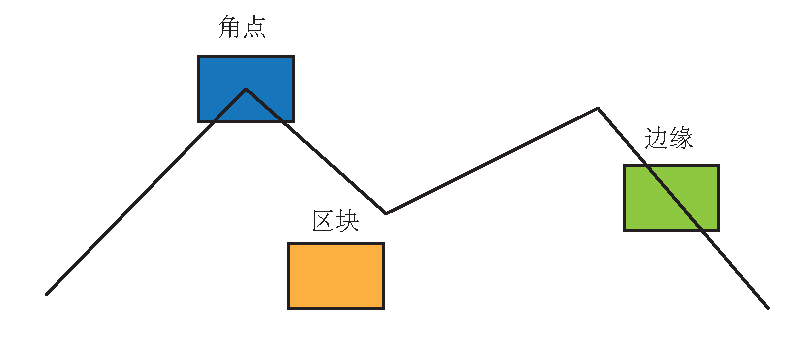
\includegraphics[width=0.8\linewidth]{vo1/corner-flat-line}\\
    \caption{可以作为图像特征的部分:角点、边缘、区块。}
    \label{fig:corner-feature}
\end{figure}

特征点由\textbf{关键点}(Key-point)和\textbf{描述子}(Descriptor)两部分组成。比如,当我们说“在一张图像中计算SIFT特征点”,是指“提取SIFT关键点,并计算SIFT描述子”两件事情。关键点是指该特征点在图像里的位置,有些特征点还具有朝向、大小等信息。描述子通常是一个向量,按照某种人为设计的方式,描述了该关键点周围像素的信息。描述子是按照“\textbf{外观相似的特征应该有相似的描述子}”的原则设计的。因此,只要两个特征点的描述子在向量空间上的距离相近,就可以认为它们是同样的特征点。

历史上,研究者们提出过许多图像特征。它们有些很精确,在相机的运动和光照变化下仍具有相似的表达,但相应地需要较大的计算量。其中,SIFT(尺度不变特征变换,Scale-Invariant Feature Transform)当属最为经典的一种。它充分考虑了在图像变换过程中出现的光照、尺度、旋转等变化,但随之而来的是极大的计算量。由于整个SLAM过程中图像特征的提取与匹配仅仅是诸多环节中的一个,到目前(2016年)为止,普通PC的CPU还无法实时地计算SIFT特征,进行定位与建图\footnote{这里是指30Hz的实时速度。}。所以在SLAM中我们甚少使用这种“奢侈”的图像特征。

另一些特征,则考虑适当降低精度和鲁棒性,以提升计算的速度。例如,FAST关键点属于计算特别快的一种特征点(注意这里“关键点”的表述,说明它没有描述子),而ORB(Oriented FAST and Rotated BRIEF)特征则是目前看来非常具有代表性的实时图像特征。它改进了FAST检测子\textsuperscript{\cite{Rosten2006}}不具有方向性的问题,并采用速度极快的二进制描述子BRIEF\textsuperscript{\cite{calonder2010brief}},使整个图像特征提取的环节大大加速。根据作者在论文中所述测试,在同一幅图像中同时提取约1000个特征点的情况下,ORB约要花费15.3ms,SURF约花费217.3ms,SIFT约花费5228.7ms。由此可以看出,ORB在保持了特征子具有旋转、尺度不变性的同时,速度方面提升明显,对于实时性要求很高的SLAM来说是一个很好的选择。

大部分特征提取都具有较好的并行性,可以通过GPU等设备来加速计算。经过GPU加速后的SIFT,就可以满足实时计算要求。但是,引入GPU将带来整个SLAM成本的提升。由此带来的性能提升是否足以抵去付出的计算成本,需要系统的设计人员仔细考量。

显然,计算机视觉领域存在大量的特征点种类,我们不可能在书中一一介绍。在目前的SLAM方案中,ORB是质量与性能之间较好的折中,因此,我们以ORB为代表介绍提取特征的整个过程。如果读者对特征提取和匹配算法感兴趣,我们建议阅读这方面的相关书籍\cite{Nixon2012}。

\subsection{ORB特征}

ORB特征亦由\textbf{关键点}和\textbf{描述子}两部分组成。它的关键点称为“Oriented FAST”,是一种改进的FAST角点,关于什么是FAST角点我们将在下文介绍。它的描述子称为BRIEF(Binary Robust Independent Elementary Feature)。因此,提取ORB特征分为如下两个步骤:
\begin{enumerate}
\item FAST角点提取:找出图像中的“角点”。相较于原版的FAST,ORB中计算了特征点的主方向,为后续的BRIEF描述子增加了旋转不变特性。
\item BRIEF描述子:对前一步提取出特征点的周围图像区域进行描述。ORB对BRIEF进行了一些改进,主要是指在BRIEF中使用了先前计算的方向信息。
\end{enumerate}

下面分别介绍FAST和BRIEF。
\subsubsection{FAST关键点}

FAST是一种角点,主要检测局部像素灰度变化明显的地方,以速度快著称。它的思想是:如果一个像素与邻域的像素差别较大(过亮或过暗),那么它更可能是角点。相比于其他角点检测算法,FAST只需比较像素亮度的大小,十分快捷。它的检测过程如下(见\autoref{fig:fastcorner}~):

\begin{enumerate}
\item 在图像中选取像素$p$,假设它的亮度为$I_{p}$。
\item 设置一个阈值$T$(比如,$I_{p}$的20\%)。
\item 以像素$p$为中心,选取半径为3的圆上的16个像素点。
\item 假如选取的圆上有连续的$N$个点的亮度大于$I_{p}+T$或小于$I_{p}-T$,那么像素$p$可以被认为是特征点($N$通常取12,即为FAST-12。其他常用的$N$取值为9和11,它们分别被称为FAST-9和FAST-11)。
\item 循环以上四步,对每一个像素执行相同的操作。
\end{enumerate}

在FAST-12算法中,为了更高效,可以添加一项预测试操作,以快速地排除绝大多数不是角点的像素。具体操作为,对于每个像素,直接检测邻域圆上的第1, 5, 9, 13个像素的亮度。只有当这4个像素中有3个同时大于$I_{p}+T$或小于$I_{p}-T$时,当前像素才有可能是一个角点,否则应该直接排除。这样的预测试操作大大加速了角点检测。此外,原始的FAST角点经常出现“扎堆”的现象。所以在第一遍检测之后,还需要用非极大值抑制(Non-maximal suppression),在一定区域内仅保留响应极大值的角点,避免角点集中的问题。

\begin{figure}[!ht]
	\centering
	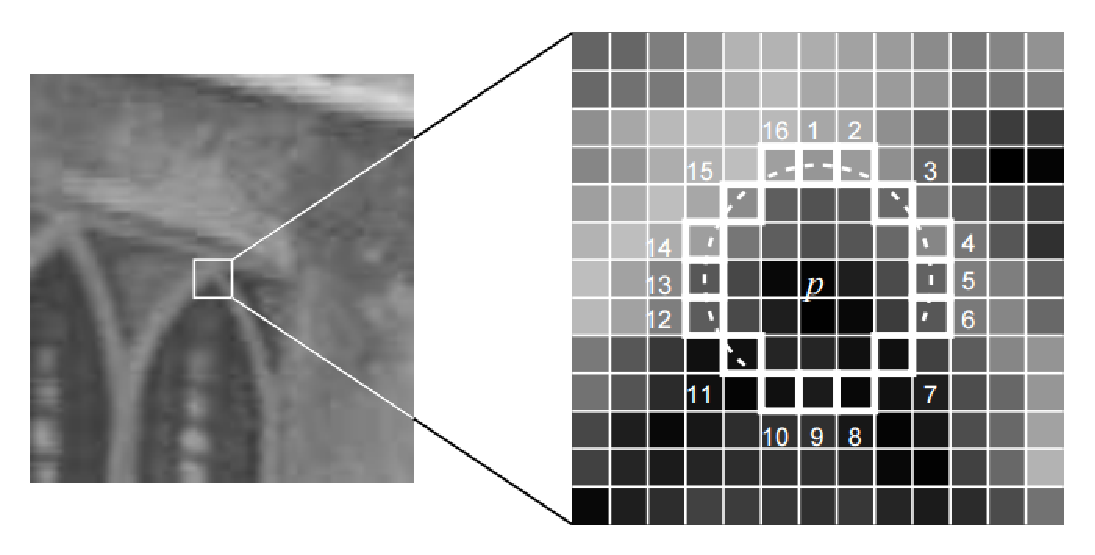
\includegraphics[width=0.9\linewidth]{vo1/fast-corner}
	\caption{FAST特征点\textsuperscript{\cite{Rosten2006}}。}
	\label{fig:fastcorner}
\end{figure}

FAST特征点的计算仅仅是比较像素间亮度的差异所所以速度非常快,但它也有重复性不强,分布不均匀的缺点。此外,FAST角点不具有方向信息。同时,由于它固定取半径为3的圆,存在尺度问题:远处看着像是角点的地方,接近后看可能就不是角点了。针对FAST角点不具有方向性和尺度的弱点,ORB添加了尺度和旋转的描述。尺度不变性由构建图像金字塔\footnote{金字塔是指对图像进行不同层次的降采样,以获得不同分辨率的图像。},并在金字塔的每一层上检测角点来实现。而特征的旋转是由灰度质心法(Intensity Centroid)实现的。

金字塔时计算图视觉中常用的一种处理方法,示意图见\autoref{fig:pyramid}。金字塔底层是原始图像。每往上一层,就对图像进行一个固定倍率的缩放,这样我们就有了不同分辨率的图像。较小的图像可以看成是远处看过来的场景。在特征匹配算法中,我们可以匹配不同层上的图像,从而实现尺度不变性。例如,如果相机在后退,那么我们应该能够在上一个图像金字塔的上层和下一个图像的下层中找到匹配。

\begin{figure}[!t]
    \centering
    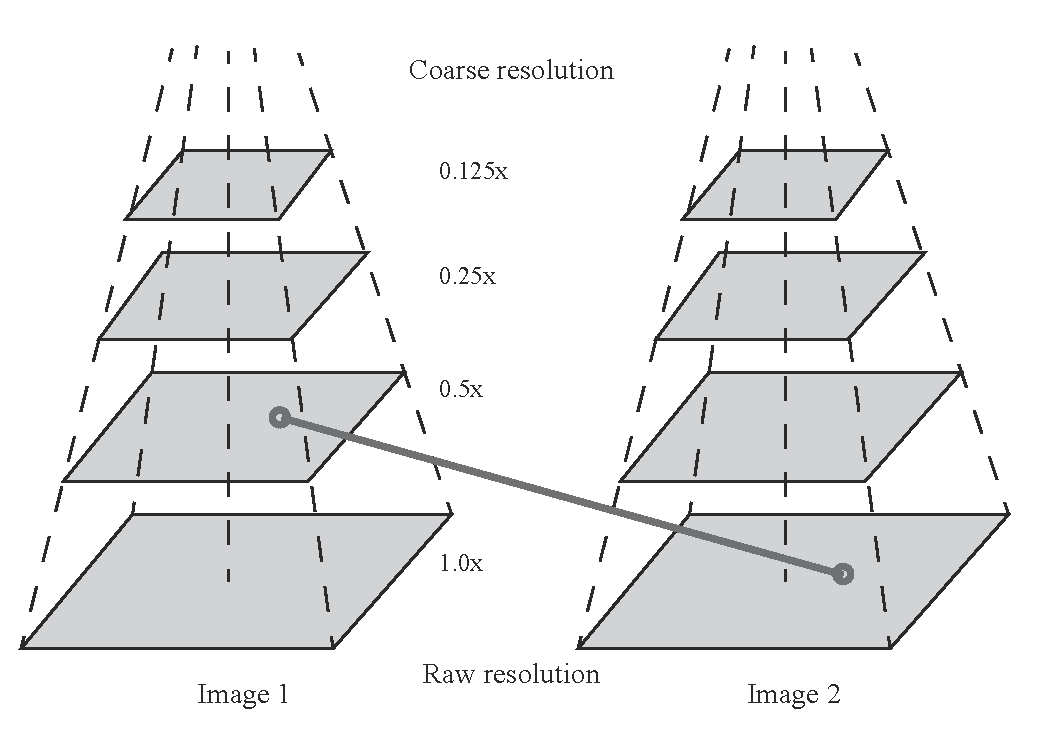
\includegraphics[width=0.9\linewidth]{vo1/pyramid}\\
    \caption{使用金字塔可以匹配不同缩放倍率下的图像。}
    \label{fig:pyramid}
\end{figure}

在旋转方面,我们计算特征点附近的图像灰度质心。所谓质心是指以图像块灰度值作为权重的中心。其具体操作步骤如下\textsuperscript{\cite{Rosin1999}}:
\begin{enumerate}
\item 在一个小的图像块$B$中,定义图像块的矩为
\[
m_{pq}=\sum_{x,y \in B}x^{p}y^{q}I(x,y), \quad p, q = \{0,1\}.
\]
\item 通过矩可以找到图像块的质心:
\[
C=(\frac{m_{10}}{m_{00}},\frac{m_{01}}{m_{00}}).
\]
\item 连接图像块的几何中心$O$与质心$C$,得到一个方向向量$\overrightarrow{OC}$,于是特征点的方向可以定义为
\[
\theta = \arctan(m_{01}/m_{10}).
\]
\end{enumerate}
通过以上方法,FAST角点便具有了尺度与旋转的描述,从而大大提升了其在不同图像之间表述的鲁棒性。所以在ORB中,把这种改进后的FAST称为Oriented FAST。

\subsubsection{BRIEF描述子}
在提取Oriented FAST关键点后,我们对每个点计算其描述子。ORB使用改进的BRIEF特征描述。我们先来介绍一下BRIEF是什么。

BRIEF是一种\textbf{二进制}描述子,其描述向量由许多个0和1组成,这里的0和1编码了关键点附近两个随机像素(比如$p$和$q$)的大小关系:如果$p$比$q$大,则取1,反之就取0。如果我们取了128个这样的$p,q$,最后就得到128维由0、1组成的向量\textsuperscript{\cite{calonder2010brief}}。BRIEF使用了随机选点的比较,速度非常快,而且由于使用了二进制表达,存储起来也十分方便,适用于实时的图像匹配。原始的BRIEF描述子不具有旋转不变性,因此在图像发生旋转时容易丢失。而ORB在FAST特征点提取阶段计算了关键点的方向,所以可以利用方向信息,计算了旋转之后的“Steer BRIEF”特征使ORB的描述子具有较好的旋转不变性。

由于考虑到了旋转和缩放,使得ORB在平移、旋转和缩放的变换下仍有良好的表现。同时,FAST和BREIF的组合也非常高效,使得ORB特征在实时SLAM中非常受欢迎。我们在\autoref{fig:ORB}~中展示了一张图像提取ORB之后的结果,下面来介绍如何在不同的图像之间进行特征匹配。

\begin{figure}[!htp]
    \centering
    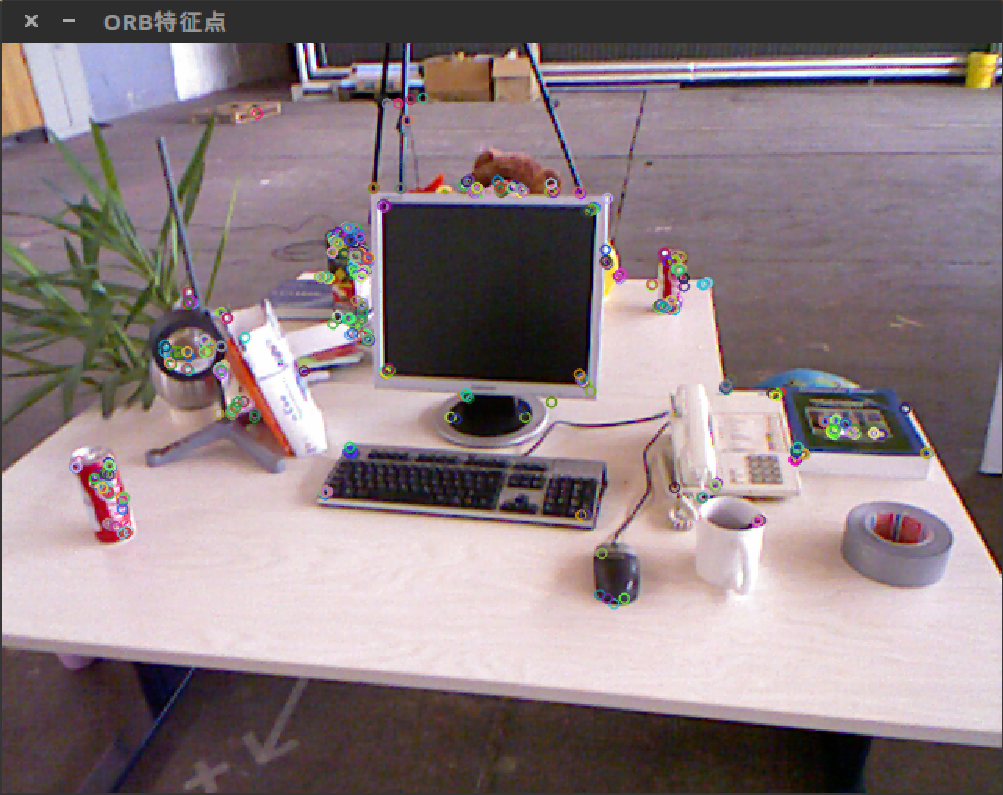
\includegraphics[width=0.9\linewidth]{vo1/feature}\\
    \caption{OpenCV提供的ORB特征点检测结果。}
    \label{fig:ORB}
\end{figure}

\subsection{特征匹配}

特征匹配(如\autoref{fig:feature-matching}~所示)是视觉SLAM中极为关键的一步,宽泛地说,特征匹配解决了SLAM中的数据关联问题(data association),即确定当前看到的路标与之前看到的路标之间的对应关系。通过对图像与图像或者图像与地图之间的描述子进行准确匹配,我们可以为后续的姿态估计、优化等操作减轻大量负担。然而,由于图像特征的局部特性,误匹配的情况广泛存在,而且长期以来一直没有得到有效解决,目前已经成为视觉SLAM中制约性能提升的一大瓶颈。部分原因是场景中经常存在大量的重复纹理,使得特征描述非常相似。在这种情况下,仅利用局部特征解决误匹配是非常困难的。

\begin{figure}[!htp]
    \centering
    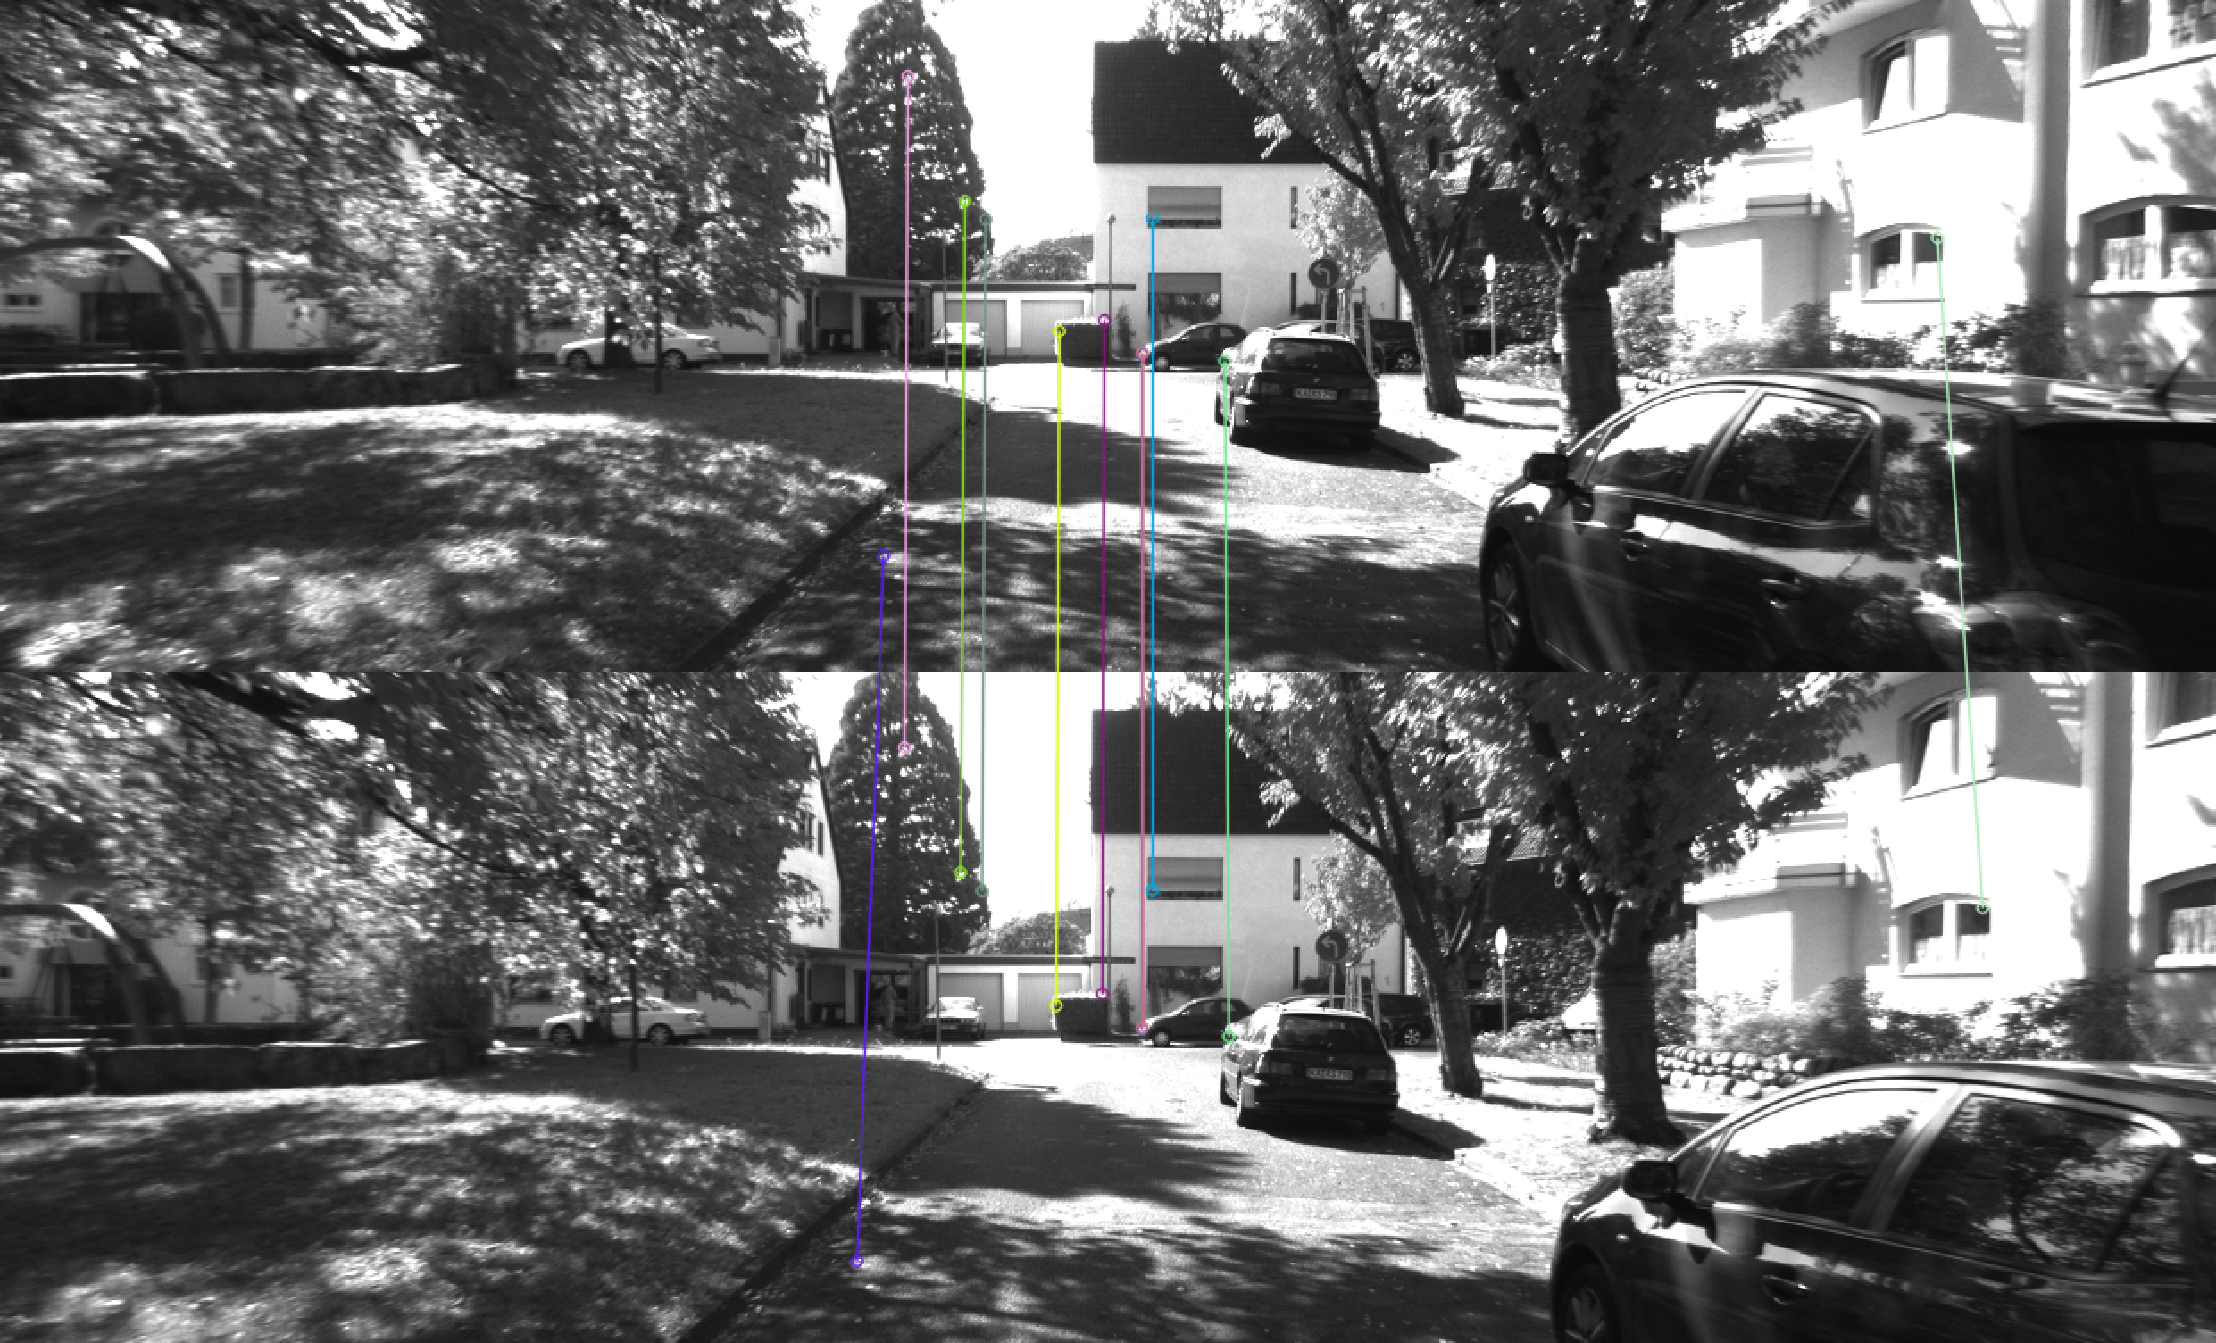
\includegraphics[width=0.9\linewidth]{vo1/feature-matching}
    \caption{两帧图像间的特征匹配。}
    \label{fig:feature-matching}
\end{figure}

不过,让我们先来看正确匹配的情况,等做完实验再回头去讨论误匹配问题。考虑两个时刻的图像。如果在图像$I_{t}$中提取到特征点$ x_{t}^{m}, m=1,2,...,M$,在图像$I_{t+1}$中提取到特征点$x_{t+1}^{n}, n=1,2,...,N$,如何寻找这两个集合元素的对应关系呢?最简单的特征匹配方法就是\textbf{暴力匹配(Brute-Force Matcher)}。即对每一个特征点$x_{t}^{m}$与所有的$x_{t+1}^{n}$测量描述子的距离,然后排序,取最近的一个作为匹配点。描述子距离表示了两个特征之间的\textbf{相似程度},不过在实际运用中还可以取不同的距离度量范数。对于浮点类型的描述子,使用欧氏距离进行度量即可。而对于二进制的描述子(比如BRIEF这样的),我们往往使用汉明距离(Hamming distance)作为度量——两个二进制串之间的汉明距离,指的是其\textbf{不同位数的个数}。

然而,当特征点数量很大时,暴力匹配法的运算量将变得很大,特别是当想要匹配某个帧和一张地图的时候。这不符合我们在SLAM中的实时性需求。此时\textbf{快速近似最近邻(FLANN)}算法更加适合于匹配点数量极多的情况。由于这些匹配算法理论已经成熟,而且实现上也已集成到OpenCV,所以这里就不再描述它的技术细节了。感兴趣的读者可以参考阅读文献\cite{Muja2009}。

\section{实践:特征提取和匹配}
\begin{figure}[!htp]
	\centering
	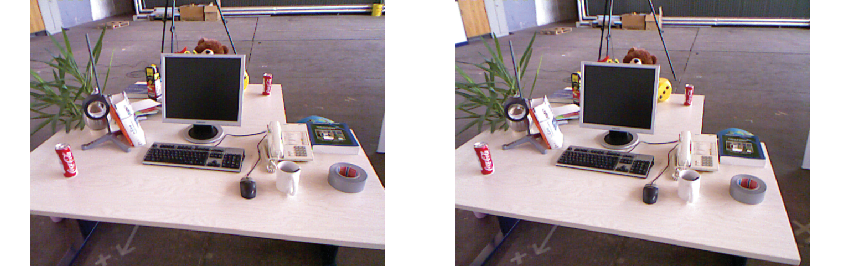
\includegraphics[width=0.9\linewidth]{vo1/exp1-images.pdf}
	\caption{实验使用的两帧图像。}
	\label{fig:exp1-images}
\end{figure}

OpenCV已经集成了多数主流的图像特征,我们可以很方便地进行调用。下面我们来完成两个实验:第一个实验中,我们演示使用OpenCV进行ORB的特征匹配;第二个实验中,我们演示如何根据前面介绍的原理,手写一个简单的ORB特征。通过手写的过程,读者可以更加清楚地理解ORB的计算过程,并类推到其他特征上去。

\subsection{OpenCV的ORB特征}
首先我们调用OpenCV来提取和匹配ORB。我为此实验准备了两张图像,位于slambook2/ch7/下的1.png和2.png,如\autoref{fig:exp1-images}~所示。它们是来自公开数据集\cite{Sturm2012}中的两张图像,我们看到相机发生了微小的运动。本节程序演示如何提取ORB特征并进行匹配。下一小节中,我们将演示如何用匹配结果来估计相机运动。

下面程序演示了ORB的使用方法:
\begin{lstlisting}[language=c++,caption=slambook2/ch7/orb_cv.cpp]
#include <iostream>
#include <opencv2/core/core.hpp>
#include <opencv2/features2d/features2d.hpp>
#include <opencv2/highgui/highgui.hpp>
#include <chrono>

using namespace std;
using namespace cv;

int main(int argc, char **argv) {
    if (argc != 3) {
        cout << "usage: feature_extraction img1 img2" << endl;
        return 1;
    }
    //-- 读取图像
    Mat img_1 = imread(argv[1], CV_LOAD_IMAGE_COLOR);
    Mat img_2 = imread(argv[2], CV_LOAD_IMAGE_COLOR);
    assert(img_1.data != nullptr && img_2.data != nullptr);
    
    //-- 初始化
    std::vector<KeyPoint> keypoints_1, keypoints_2;
    Mat descriptors_1, descriptors_2;
    Ptr<FeatureDetector> detector = ORB::create();
    Ptr<DescriptorExtractor> descriptor = ORB::create();
    Ptr<DescriptorMatcher> matcher = DescriptorMatcher::create("BruteForce-Hamming");
    
    //-- 第一步:检测 Oriented FAST 角点位置
    chrono::steady_clock::time_point t1 = chrono::steady_clock::now();
    detector->detect(img_1, keypoints_1);
    detector->detect(img_2, keypoints_2);
    
    //-- 第二步:根据角点位置计算 BRIEF 描述子
    descriptor->compute(img_1, keypoints_1, descriptors_1);
    descriptor->compute(img_2, keypoints_2, descriptors_2);
    chrono::steady_clock::time_point t2 = chrono::steady_clock::now();
    chrono::duration<double> time_used = chrono::duration_cast<chrono::duration<double>>(t2 - t1);
    cout << "extract ORB cost = " << time_used.count() << " seconds. " << endl;
    
    Mat outimg1;
    drawKeypoints(img_1, keypoints_1, outimg1, Scalar::all(-1), DrawMatchesFlags::DEFAULT);
    imshow("ORB features", outimg1);
    
    //-- 第三步:对两幅图像中的BRIEF描述子进行匹配,使用 Hamming 距离
    vector<DMatch> matches;
    t1 = chrono::steady_clock::now();
    matcher->match(descriptors_1, descriptors_2, matches);
    t2 = chrono::steady_clock::now();
    time_used = chrono::duration_cast<chrono::duration<double>>(t2 - t1);
    cout << "match ORB cost = " << time_used.count() << " seconds. " << endl;
    
    //-- 第四步:匹配点对筛选
    // 计算最小距离和最大距离
    auto min_max = minmax_element(matches.begin(), matches.end(),
        [](const DMatch &m1, const DMatch &m2) { return m1.distance < m2.distance; });
    double min_dist = min_max.first->distance;
    double max_dist = min_max.second->distance;
    
    printf("-- Max dist : %f \n", max_dist);
    printf("-- Min dist : %f \n", min_dist);
    
    //当描述子之间的距离大于两倍的最小距离时,即认为匹配有误.但有时候最小距离会非常小,设置一个经验值30作为下限.
    std::vector<DMatch> good_matches;
    for (int i = 0; i < descriptors_1.rows; i++) {
        if (matches[i].distance <= max(2 * min_dist, 30.0)) {
            good_matches.push_back(matches[i]);
        }
    }
    
    //-- 第五步:绘制匹配结果
    Mat img_match;
    Mat img_goodmatch;
    drawMatches(img_1, keypoints_1, img_2, keypoints_2, matches, img_match);
    drawMatches(img_1, keypoints_1, img_2, keypoints_2, good_matches, img_goodmatch);
    imshow("all matches", img_match);
    imshow("good matches", img_goodmatch);
    waitKey(0);
    
    return 0;
}
\end{lstlisting}

运行此程序(需要输入两个图像位置),将输出运行结果:
\begin{lstlisting}[language=sh,caption=终端输入:]
% build/orb_cv 1.png 2.png
extract ORB cost = 0.0229183 seconds. 
match ORB cost = 0.000751868 seconds.
-- Max dist : 95.000000 
-- Min dist : 4.000000 
\end{lstlisting}

\autoref{fig:exp1-results}~显示了例程的运行结果。我们看到未筛选的匹配中带有大量的误匹配。经过一次筛选之后,匹配数量减少了许多,但大多数匹配都是正确的。这里,筛选的依据是\textbf{汉明距离小于最小距离的两倍},这是一种工程上的经验方法,不一定有理论依据。不过,尽管在示例图像中能够筛选出正确的匹配,但我们仍然不能保证在所有其他图像中得到的匹配都是正确的。因此,在后面的运动估计中,还需要使用去除误匹配的算法。在我的机器上,ORB提取花费了22.9毫秒(两张图像),匹配花费了0.75毫秒,可见大部分计算量花在了特征提取上。

\begin{figure}[!htp]
	\centering
	\includegraphics[width=1.0\linewidth]{vo1/exp1-result}
	\caption{特征提取与匹配结果。}
	\label{fig:exp1-results} 
\end{figure}

\subsection{手写ORB特征}
下面我们演示手写ORB特征的方法。这部分代码比较多,书上只展示核心部分的代码,其余的周边代码请读者从代码库中获取。
\begin{lstlisting}[language=c++,caption=slambook2/ch7/orb_self.cpp(片段)]
typedef vector<uint32_t> DescType;
// ... 省略图片读取部分代码和测试代码
// compute the descriptor
void ComputeORB(const cv::Mat &img, vector<cv::KeyPoint> &keypoints, vector<DescType> &descriptors) {
    const int half_patch_size = 8;
    const int half_boundary = 16;
    int bad_points = 0;
    for (auto &kp: keypoints) {
        if (kp.pt.x < half_boundary || kp.pt.y < half_boundary ||
        kp.pt.x >= img.cols - half_boundary || kp.pt.y >= img.rows - half_boundary) {
            // outside
            bad_points++;
            descriptors.push_back({});
            continue;
        }
    
        float m01 = 0, m10 = 0;
        for (int dx = -half_patch_size; dx < half_patch_size; ++dx) {
            for (int dy = -half_patch_size; dy < half_patch_size; ++dy) {
                uchar pixel = img.at<uchar>(kp.pt.y + dy, kp.pt.x + dx);
                m01 += dx * pixel;
                m10 += dy * pixel;
            }
        }
    
        // angle should be arc tan(m01/m10);
        float m_sqrt = sqrt(m01 * m01 + m10 * m10);
        float sin_theta = m01 / m_sqrt;
        float cos_theta = m10 / m_sqrt;
        
        // compute the angle of this point
        DescType desc(8, 0);
        for (int i = 0; i < 8; i++) {
            uint32_t d = 0;
            for (int k = 0; k < 32; k++) {
                int idx_pq = i * 8 + k;
                cv::Point2f p(ORB_pattern[idx_pq * 4], ORB_pattern[idx_pq * 4 + 1]);
                cv::Point2f q(ORB_pattern[idx_pq * 4 + 2], ORB_pattern[idx_pq * 4 + 3]);
        
                // rotate with theta
                cv::Point2f pp = cv::Point2f(cos_theta * p.x - sin_theta * p.y, sin_theta * p.x + cos_theta * p.y) + kp.pt;
                cv::Point2f qq = cv::Point2f(cos_theta * q.x - sin_theta * q.y, sin_theta * q.x + cos_theta * q.y) + kp.pt;
                if (img.at<uchar>(pp.y, pp.x) < img.at<uchar>(qq.y, qq.x)) {
                    d |= 1 << k;
                }
            }
            desc[i] = d;
        }
        descriptors.push_back(desc);
    }
    
    cout << "bad/total: " << bad_points << "/" << keypoints.size() << endl;
}

// brute-force matching
void BfMatch(
    const vector<DescType> &desc1, const vector<DescType> &desc2, vector<cv::DMatch> &matches) {
    const int d_max = 40;
    
    for (size_t i1 = 0; i1 < desc1.size(); ++i1) {
        if (desc1[i1].empty()) continue;
        cv::DMatch m{i1, 0, 256};
        for (size_t i2 = 0; i2 < desc2.size(); ++i2) {
            if (desc2[i2].empty()) continue;
            int distance = 0;
            for (int k = 0; k < 8; k++) {
                distance += _mm_popcnt_u32(desc1[i1][k] ^desc2[i2][k]);
            }
            if (distance < d_max && distance < m.distance) {
                m.distance = distance;
                m.trainIdx = i2;
            }
        }
        if (m.distance < d_max) {
            matches.push_back(m);
        }
    }
}
\end{lstlisting}
这个演示中我们只展示ORB的计算代码和匹配代码。在计算中,我们用256位的二进制描述,即对应到8个32位的unsigned int数据,用typedef将它表示成DescType。然后,我们根据前面介绍的原理计算FAST特征点的角度,再使用该角度计算描述子。此代码中通过三角函数的原理回避了复杂的$\arctan$以及$\sin$、$\cos$计算,从而达到加速的效果。在BfMatch函数中,我们还使用了SSE指令集中的\_mm\_popcnt\_u32函数来计算一个unsigned int变量中1的个数,从而达到计算汉明距离的效果。该段程序的运行结果如下,匹配结果如\autoref{fig:matches}所示:

\begin{lstlisting}[language=sh,caption=终端输出:]
bad/total: 43/638
bad/total: 8/595
extract ORB cost = 0.00390721 seconds.
match ORB cost = 0.000862984 seconds.
matches: 51
\end{lstlisting}

\begin{figure}[!htp]
    \centering
    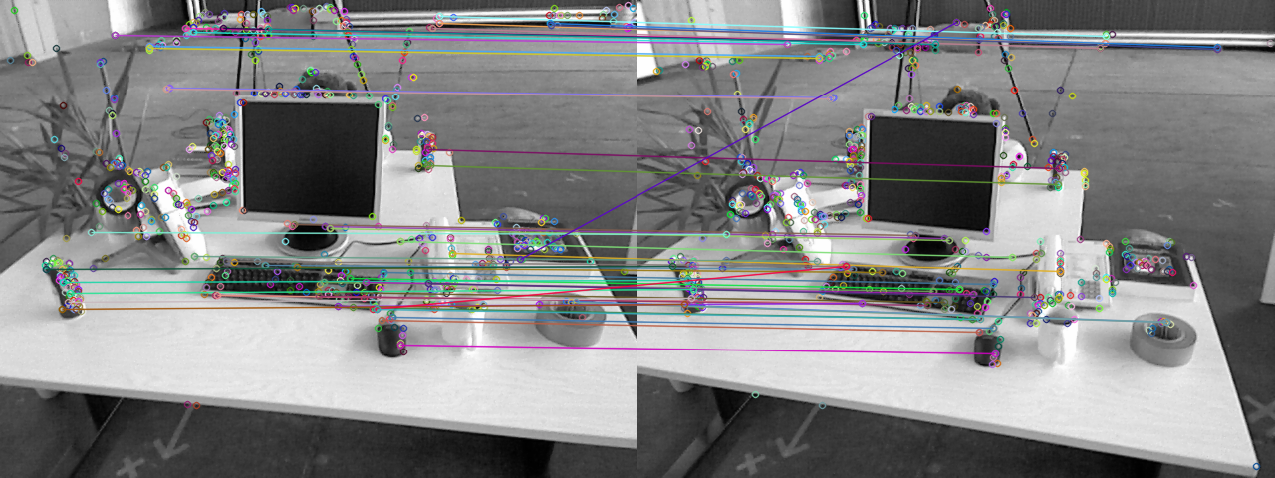
\includegraphics[width=0.8\linewidth]{vo1/matches}
    \caption{匹配结果}
    \label{fig:matches}
\end{figure}

可见,这个程序中,ORB的提取只需要3.9毫秒,匹配只需0.86毫秒。我们通过一些简单的算法修改,对ORB的提取加速了5.8倍。请读者注意,编译这个程序需要你的CPU支持SSE指令集,这应该在绝大多数现代的家用CPU上都已经支持。如果我们能够对提取特征部分进一步并行化处理,算法还可以有加速的空间。

\subsection{计算相机运动}
我们已经有了匹配好的点对,接下来,我们要根据点对来估计相机的运动。这里由于相机的原理不同,情况发生了变化:

\begin{enumerate}
	\item 当相机为单目时,我们只知道2D的像素坐标,因而问题是根据\textbf{两组2D点}估计运动。该问题用\textbf{对极几何}来解决。
	\item 当相机为双目、RGB-D时,或者通过某种方法得到了距离信息,那么问题就是根据\textbf{两组3D点}估计运动。该问题通常用ICP来解决。
	\item 如果一组为3D,一组为2D,即,我们得到了一些3D点和它们在相机的投影位置,也能估计相机的运动。该问题通过\textbf{PnP}求解。
\end{enumerate}

因此,下面几节就来介绍这三种情形下的相机运动估计。我们将从信息最少的2D−2D情形出发,看看它如何求解,求解过程又有哪些麻烦的问题。

\section{2D−2D: 对极几何}
\label{sec:epipolar-geometry}

\subsection{对极约束}

现在,假设我们从两张图像中得到了一对配对好的特征点,如\autoref{fig:doubleview}~所示。如果有若干对这样的匹配点,就可以通过这些二维图像点的对应关系,恢复出在两帧之间摄像机的运动。这里“若干对”具体是多少对呢?我们会在下文介绍。下面先来看看两个图像当中的匹配点有什么几何关系。

\begin{figure}[!htp]
	\centering
	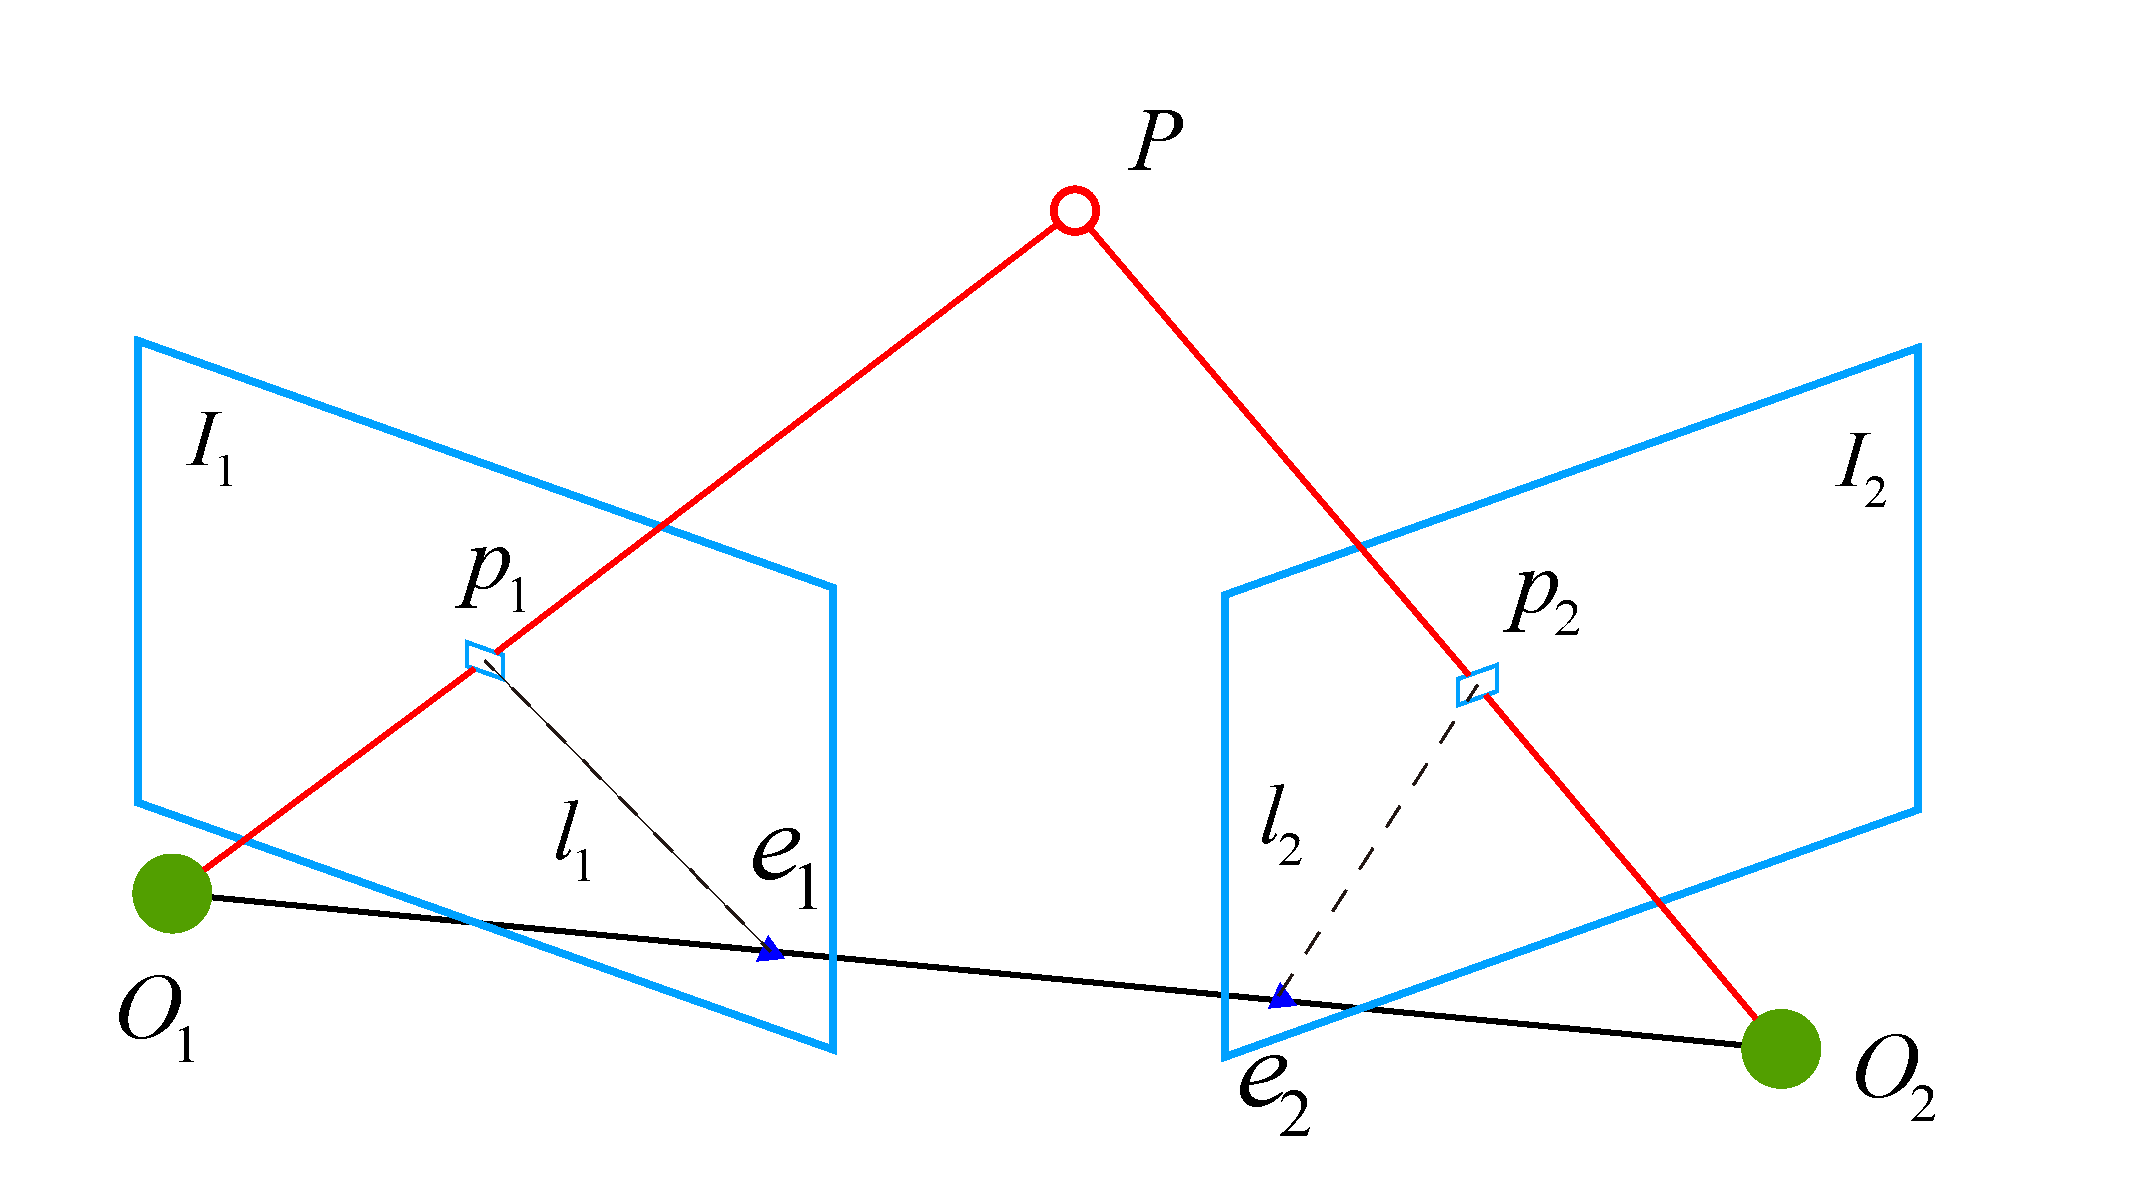
\includegraphics[width=0.6\linewidth]{vo1/fundamental}
	\caption{对极几何约束。}
	\label{fig:doubleview}
\end{figure}

以\autoref{fig:doubleview}~为例,我们希望求取两帧图像$I_{1}, I_{2}$之间的运动,设第一帧到第二帧的运动为$\bm{R}, \bm{t}$。两个相机中心分别为$O_{1}, O_{2}$。现在,考虑$I_{1}$中有一个特征点$p_{1}$,它在$I_{2}$中对应着特征点$p_{2}$。我们知道两者是通过特征匹配得到的。如果匹配正确,说明它们确实是\textbf{同一个空间点在两个成像平面上的投影}。这里需要一些术语来描述它们之间的几何关系。首先,连线$\overrightarrow{O_{1}p_{1}}$和连线$\overrightarrow{O_{2}p_{2}}$在三维空间中会相交于点$P$。这时候点$O_{1},O_{2},P$三个点可以确定一个平面,称为\textbf{极平面(Epipolar plane)}。$O_{1}O_{2}$连线与像平面$I_{1},I_{2}$的交点分别为$e_{1},e_{2}$。$e_{1},e_{2}$称为\textbf{极点(Epipoles)},$O_{1}O_{2}$被称为\textbf{基线(Baseline)}。我们称极平面与两个像平面$I_{1}, I_{2}$之间的相交线$l_{1},l_{2}$为\textbf{极线(Epipolar line)}。

直观讲,从第一帧的角度看,射线$\overrightarrow{O_1 p_1}$是\textbf{某个像素可能出现的空间位置}——因为该射线上的所有点都会投影到同一个像素点。同时,如果不知道$P$的位置,那么当我们在第二幅图像上看时,连线$\overrightarrow{e_2 p_2}$(也就是第二幅图像中的极线)就是$P$可能出现的投影的位置,也就是射线$\overrightarrow{O_1 p_1}$在第二个相机中的投影。现在,由于我们通过特征点匹配确定了$p_2$的像素位置,所以能够推断$P$的空间位置,以及相机的运动。要提醒读者的是,\textbf{这多亏了正确的特征匹配}。如果没有特征匹配,我们就没法确定$p_2$到底在极线的哪个位置了。那时,就必须在极线上搜索以获得正确的匹配,这将在第12讲中提到。

现在,我们从代数角度来看一下这里的几何关系。在第一帧的坐标系下,设$P$的空间位置为
\[
\bm{P}=[X,Y,Z]^\mathrm{T}.
\]
根据第5讲介绍的针孔相机模型,我们知道两个像素点$\bm{p}_1,\bm{p}_2$的像素位置为
\begin{equation}
s_1 {\bm{p}_1} = \bm{KP},\quad s_2 \bm{p}_2 = \bm{K}\left( \bm{RP + t} \right).
\end{equation}

这里$\bm{K}$为相机内参矩阵,$\bm{R}, \bm{t}$为两个坐标系的相机运动。具体来说,这里计算的是$\bm{R}_{21}$和$\bm{t}_{21}$,因为它们把第一个坐标系下的坐标转换到第二个坐标系下。如果我们愿意,也可以把它们写成李代数形式。

有时候,我们会使用齐次坐标表示像素点。在使用齐次坐标时,一个向量将等于它自身乘上任意的非零常数。这通常用于表达一个投影关系。例如$s_1 \bm{p}_1$和$\bm{p}_1$成投影关系,它们在齐次坐标的意义下是相等的。我们称这种相等关系为\textbf{尺度意义下相等}(equal up to a scale),记作:
\begin{equation}
s\bm{p} \simeq \bm{p}.
\end{equation}
那么,上述两个投影关系可写为:
\begin{equation}
 {\bm{p}_1} \simeq \bm{KP},\quad \bm{p}_2 \simeq \bm{K}\left( \bm{RP + t} \right).
\end{equation}

现在,取:
\begin{equation}
{\bm{x}_1} = {\bm{K}^{ - 1}}{\bm{p}_1}, \quad {\bm{x}_2} = {\bm{K}^{ - 1}}{\bm{p}_2}.
\end{equation}

这里的$\bm{x}_1, \bm{x}_2$是两个像素点的归一化平面上的坐标。代入上式,得:
\begin{equation}
{\bm{x}_2} \simeq \bm{R} {\bm{x}_1} + \bm{t}.
\end{equation}

两边同时左乘$\bm{t}^\wedge$。回忆$^\wedge$的定义,这相当于两侧同时与$\bm{t}$做外积:
\begin{equation}
\bm{t}^\wedge \bm{x}_2 \simeq \bm{t}^\wedge \bm{R} \bm{x}_1.
\end{equation}

然后,两侧同时左乘$\bm{x}_2^\mathrm{T}$:
\begin{equation}
\bm{x}_2^\mathrm{T} \bm{t}^\wedge \bm{x}_2 \simeq \bm{x}_2^\mathrm{T} \bm{t}^\wedge \bm{R} \bm{x}_1.
\end{equation}

观察等式左侧,$\bm{t}^\wedge \bm{x}_2$是一个与$\bm{t}$和$\bm{x}_2$都垂直的向量。把它再和$\bm{x}_2$做内积时,将得到0。由于等式左侧严格为零,那么乘以任意非零常数之后也为零,于是我们可以把$\simeq$写成通常的等号。因此,我们就得到了一个简洁的式子:
\begin{equation}
 \bm{x}_2^\mathrm{T} \bm{t}^\wedge \bm{R} \bm{x}_1 = 0.
\end{equation}

重新代入$\bm{p}_1, \bm{p}_2$,有:
\begin{equation}
\bm{p}_2^\mathrm{T} \bm{K}^{-\mathrm{T}} \bm{t}^\wedge \bm{R} \bm{K}^{-1} \bm{p}_1  = 0.
\end{equation}

这两个式子都称为\textbf{对极约束},它以形式简洁著名。它的几何意义是$O_1, P, O_2$三者共面。对极约束中同时包含了平移和旋转。我们把中间部分记作两个矩阵:基础矩阵(Fundamental Matrix)$\bm{F}$和本质矩阵(Essential Matrix)$\bm{E}$,于是可以进一步简化对极约束:
\begin{equation}
\bm{E} = \bm{t}^ \wedge \bm{R}, \quad \bm{F} = \bm{K}^{ -\mathrm{T}} \bm{E} {\bm{K}^{ - 1}}, \quad \bm{x}_2^\mathrm{T} \bm{E} {\bm{x}_1} = \bm{p}_2^\mathrm{T} \bm{F} {\bm{p}_1} = 0.
\end{equation}

对极约束简洁地给出了两个匹配点的空间位置关系。于是,相机位姿估计问题变为以下两步:

\begin{enumerate}
	\item 根据配对点的像素位置求出$\bm{E}$或者$\bm{F}$。
	\item 根据$\bm{E}$或者$\bm{F}$求出$\bm{R}, \bm{t}$。
\end{enumerate}

由于$\bm{E}$和$\bm{F}$只相差了相机内参,而内参在SLAM中通常是已知的\footnote{在SfM研究中则有可能是未知而有待估计的。},所以实践当中往往使用形式更简单的$\bm{E}$。我们以$\bm{E}$为例,介绍上面两个问题如何求解。

\subsection{本质矩阵}
根据定义,本质矩阵$\bm{E} = \bm{t}^\wedge \bm{R}$。它是一个$3\times 3$的矩阵,内有9个未知数。那么,是不是任意一个$3 \times 3$的矩阵都可以被当成本质矩阵呢?从$\bm{E}$的构造方式上看,有以下值得注意的地方:

\begin{itemize}
	\item 本质矩阵是由对极约束定义的。由于对极约束是\textbf{等式为零}的约束,所以对$\bm{E}$乘以任意非零常数后,\textbf{对极约束依然满足}。我们把这件事情称为$\bm{E}$在不同尺度下是等价的。
	\item 根据$\bm{E} = \bm{t}^ \wedge \bm{R}$,可以证明\textsuperscript{\cite{Hartley2003}},本质矩阵$\bm{E}$的奇异值必定是$[\sigma, \sigma, 0]^\mathrm{T}$的形式。这称为\textbf{本质矩阵的内在性质}。
	\item 另一方面,由于平移和旋转各有3个自由度,故$\bm{t}^\wedge \bm{R}$共有6个自由度。但由于尺度等价性,故$\bm{E}$实际上有5个自由度。
\end{itemize}

$\bm{E}$具有5个自由度的事实,表明我们最少可以用5对点来求解$\bm{E}$。但是,$\bm{E}$的内在性质是一种非线性性质,在估计时会带来麻烦,因此,也可以只考虑它的\textbf{尺度等价性},使用8对点来估计$\bm{E}$——这就是经典的\textbf{八点法(Eight-point-algorithm)}\textsuperscript{\cite{Hartley1997, Longuet-Higgins1987}}。八点法只利用了$\bm{E}$的线性性质,因此可以在线性代数框架下求解。下面我们来看八点法是如何工作的。

考虑一对匹配点,它们的归一化坐标为$\bm{x}_{1}=[u_{1},v_{1},1]^\mathrm{T}$, $\bm{x}_{2}=[u_{2},v_{2},1]^{\mathrm{T}}$。根据对极约束,有:
\begin{equation}
\begin{pmatrix} 
u_{2},v_{2},1
\end{pmatrix}
\begin{pmatrix}
 e_{1} & e_{2} & e_{3}\\ 
 e_{4} & e_{5} & e_{6}\\ 
 e_{7} & e_{8} & e_{9} 
\end{pmatrix}
\begin{pmatrix} 
u_{1}\\v_{1}\\1
\end{pmatrix}
=0.
\end{equation}

我们把矩阵$\bm{E}$展开,写成向量的形式:
\[
\bm{e}= [e_{1},e_{2},e_{3},e_{4},e_{5},e_{6},e_{7},e_{8},e_{9}]^{\mathrm{T}},
\]
那么对极约束可以写成与$\bm{e}$有关的线性形式:
\begin{equation}
[u_{2}u_{1},u_{2}v_{1},u_{2},v_{2}u_{1},v_{2}v_{1},v_{2},u_{1},v_{1},1] \cdot  \bm{e}=0.
\end{equation}

同理,对于其他点对也有相同的表示。我们把所有点都放到一个方程中,变成线性方程组($u^i, v^i$表示第$i$个特征点,依此类推):
\begin{equation}
\label{Eq:eight-point}
\begin{pmatrix}
u_{2}^{1}u_{1}^{1}& u_{2}^{1}v_{1}^{1}& u_{2}^{1}& v_{2}^{1}u_{1}^{1}& v_{2}^{1}v_{1}^{1}& v_{2}^{1} &u_{1}^{1} &v_{1}^{1}&1\\
u_{2}^{2}u_{1}^{2}& u_{2}^{2}v_{1}^{2}& u_{2}^{2}& v_{2}^{2}u_{1}^{2}& v_{2}^{2}v_{1}^{2}& v_{2}^{2} &u_{1}^{2} &v_{1}^{2}&1\\
\vdots & \vdots & \vdots & \vdots & \vdots & \vdots & \vdots & \vdots \\
u_{2}^{8}u_{1}^{8}& u_{2}^{8}v_{1}^{8}& u_{2}^{8}& v_{2}^{8}u_{1}^{8}& v_{2}^{8}v_{1}^{8}& v_{2}^{8} &u_{1}^{8}&v_{1}^{8}&1\\
\end{pmatrix}
\begin{pmatrix}
e_{1}\\ e_{2}\\ e_{3}\\  e_{4}\\ e_{5}\\ e_{6}\\ e_{7}\\ e_{8}\\ e_{9}  
\end{pmatrix}
=0.
\end{equation}

这8个方程构成了一个线性方程组。它的系数矩阵由特征点位置构成,大小为$8 \times 9$。$\bm{e}$位于该矩阵的零空间中。如果系数矩阵是满秩的(即秩为8),那么它的零空间维数为1,也就是$\bm{e}$构成一条线。这与$\bm{e}$的尺度等价性是一致的。如果8对匹配点组成的矩阵满足秩为8的条件,那么$\bm{E}$的各元素就可由上述方程解得。

接下来的问题是如何根据已经估得的本质矩阵$\bm{E}$,恢复出相机的运动$\bm{R}, \bm{t}$。这个过程是由奇异值分解(SVD)得到的。设$\bm{E}$的SVD分解为
\begin{equation}
\bm{E} = \bm{U} \bm{\Sigma} \bm{V}^\mathrm{T},
\end{equation}
其中$\bm{U}, \bm{V}$为正交阵,$\bm{\Sigma}$为奇异值矩阵。根据$\bm{E}$的内在性质,我们知道$\bm{\Sigma} = \mathrm{diag}( \sigma, \sigma, 0 )$。在SVD分解中,对于任意一个$\bm{E}$,存在两个可能的$\bm{t}, \bm{R}$与它对应:
\begin{equation}
\begin{array}{l}
\bm{t}_1^ \wedge  = \bm{U}{\bm{R}_Z}(\frac{\uppi }{2}) \bm{\Sigma} {\bm{U}^\mathrm{T}}, \quad {\bm{R}_1} = \bm{U} \bm{R}_Z^\mathrm{T}(\frac{\uppi }{2}){ \bm{V}^\mathrm{T}}\\
\bm{t}_2^ \wedge  = \bm{U}{\bm{R}_Z}( - \frac{\uppi }{2})\bm{\Sigma} {\bm{U}^\mathrm{T}}, \quad  {\bm{R}_2} = \bm{U} \bm{R}_Z^\mathrm{T}( - \frac{\uppi }{2}){\bm{V}^\mathrm{T}}.
\end{array}
\end{equation}

其中$\bm{R}_Z(\frac{\uppi }{2})$表示沿$Z$轴旋转$90^\circ$得到的旋转矩阵。同时,由于$-\bm{E}$和$\bm{E}$等价,所以对任意一个$\bm{t}$取负号,也会得到同样的结果。因此,从$\bm{E}$分解到$\bm{t}, \bm{R}$时,一共存在\textbf{4个}可能的解。

\autoref{fig:epipolar-solution}~形象地展示了分解本质矩阵得到的4个解。我们已知空间点在相机(蓝色线)上的投影(红色点),想要求解相机的运动。在保持红色点不变的情况下,可以画出4种可能的情况。不过幸运的是,只有第一种解中$P$在两个相机中都具有正的深度。因此,只要把任意一点代入4种解中,检测该点在两个相机下的深度,就可以确定哪个解是正确的了。

\begin{figure}[!htp]
	\centering
	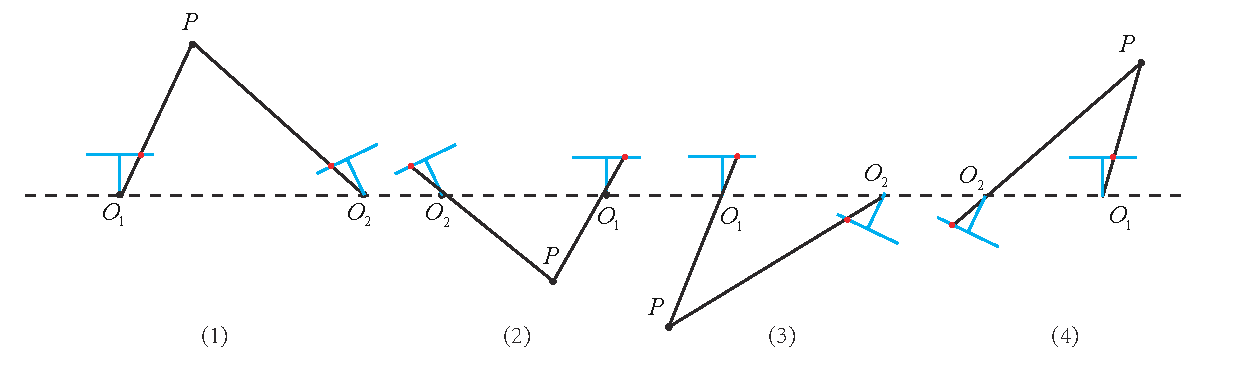
\includegraphics[width=1.0\linewidth]{vo1/epipolar-solution}
	\caption{分解本质矩阵得到的4个解。在保持投影点(红色点)不变的情况下,两个相机及空间点一共有4种可能的情况。}
	\label{fig:epipolar-solution}
\end{figure}

如果利用$\bm{E}$的内在性质,那么它只有5个自由度。所以最少可以通过5对点来求解相机运动\textsuperscript{\cite{Li2006, Nister2004a}}。然而这种做法形式复杂,从工程实现角度考虑,由于平时通常会有几十对乃至上百对的匹配点,从8对减至5对意义并不明显。为保持简单,我们这里就只介绍基本的八点法。

剩下的问题还有一个:根据线性方程解出的$\bm{E}$,可能不满足$\bm{E}$的内在性质——它的奇异值不一定为${\sigma}, {\sigma}, 0$的形式。这时,我们会刻意地把$\bm{\Sigma}$矩阵调整成上面的样子。通常的做法是,对八点法求得的$\bm{E}$进行SVD分解后,会得到奇异值矩阵$\bm{\Sigma} =  \mathrm{diag} ( \sigma_1, \sigma_2, \sigma_3)$,不妨设$\sigma_1 \geqslant \sigma_2 \geqslant \sigma_3$。取:
\begin{equation}
\bm{E} = \bm{U} \mathrm{diag} (\frac{\sigma_1+\sigma_2}{2}, \frac{\sigma_1+\sigma_2}{2}, 0) \bm{V}^\mathrm{T}.
\end{equation}
这相当于是把求出来的矩阵投影到了$\bm{E}$所在的流形上。当然,更简单的做法是将奇异值矩阵取成$\mathrm{diag} (1,1,0)$,因为$\bm{E}$具有尺度等价性,所以这样做也是合理的。

\subsection{单应矩阵}
除了基本矩阵和本质矩阵,二视图几何中还存在另一种常见的矩阵:单应矩阵(Homography)$\bm{H}$,它描述了两个平面之间的映射关系。若场景中的特征点都落在同一平面上(比如墙、地面等),则可以通过单应性来进行运动估计。这种情况在无人机携带的俯视相机或扫地机携带的顶视相机中比较常见。由于之前没有提到过单应,因此这里稍微介绍一下。

单应矩阵通常描述处于共同平面上的一些点在两张图像之间的变换关系。设图像$I_{1}$和$I_{2}$有一对匹配好的特征点$p_{1}$和$p_{2}$。这个特征点落在平面$P$上,设这个平面满足方程:
\begin{equation}
\bm{n}^\mathrm{T} \bm{P} + d = 0.
\end{equation}
稍加整理,得:
\begin{equation}
- \frac{\bm{n}^\mathrm{T} \bm{P} }{d} = 1.
\end{equation}

然后,回顾本节开头的式(7.1),得:
\begin{align*}
\bm{p}_2 &\simeq \bm{K} ( \bm{R} \bm{P} + \bm{t} ) \\ 
&\simeq \bm{K} \left( \bm{R} \bm{P} + \bm{t} \cdot (- \frac{\bm{n}^\mathrm{T} \bm{P} }{d}) \right) \\
&\simeq \bm{K} \left( \bm{R} - \frac{\bm{t} \bm{n}^\mathrm{T} }{d} \right) \bm{P} \\ 
&\simeq \bm{K} \left( \bm{R} - \frac{\bm{t} \bm{n}^\mathrm{T} }{d} \right) \bm{K}^{-1} \bm{p}_1.
\end{align*}

于是,我们得到了一个直接描述图像坐标$\bm{p}_1$和$\bm{p}_2$之间的变换,把中间这部分记为$\bm{H}$,于是:
\begin{equation}
\bm{p}_2 \simeq \bm{H} \bm{p}_1.
\end{equation}

它的定义与旋转、平移及平面的参数有关。与基础矩阵$\bm{F}$类似,单应矩阵$\bm{H}$也是一个$3 \times 3$的矩阵,求解时的思路也和$\bm{F}$类似,同样可以先根据匹配点计算$\bm{H}$,然后将它分解以计算旋转和平移。把上式展开,得:
\begin{equation}
\begin{pmatrix} 
u_{2}\\v_{2}\\1
\end{pmatrix}
\simeq
\begin{pmatrix}
 h_{1} & h_{2} & h_{3}\\ 
 h_{4} & h_{5} & h_{6}\\ 
 h_{7} & h_{8} & h_{9} 
\end{pmatrix}
\begin{pmatrix} 
u_{1}\\v_{1}\\1
\end{pmatrix}.
\end{equation}

请注意,这里的等号依然是$\simeq$而不是普通的等号,所以$\bm{H}$矩阵也可以乘以任意非零常数。我们在实际处理中可以令$h_9 = 1$(在它取非零值时)。然后根据第3行,去掉这个非零因子,于是有:
\[
\begin{aligned}
u_{2}&=\frac{h_{1}u_{1}+h_{2}v_{1}+h_{3}}{h_{7}u_{1}+h_{8}v_{1}+h_{9}}\\
v_{2}&=\frac{h_{4}u_{1}+h_{5}v_{1}+h_{6}}{h_{7}u_{1}+h_{8}v_{1}+h_{9}}.
\end{aligned}
\]
整理得:
\[
\begin{gathered}
h_{1}u_{1}+h_{2}v_{1}+h_{3}-h_{7}u_{1}u_{2}-h_{8}v_{1}u_{2}=u_{2}\\
h_{4}u_{1}+h_{5}v_{1}+h_{6}-h_{7}u_{1}v_{2}-h_{8}v_{1}v_{2}=v_{2}.
\end{gathered}
\]

这样一组匹配点对就可以构造出两项约束(事实上有三个约束,但是因为线性相关,只取前两个),于是自由度为8的单应矩阵可以通过4对匹配特征点算出(在非退化的情况下,即这些特征点不能有三点共线的情况),即求解以下的线性方程组(当$h_9 = 0$时,右侧为零):
\begin{equation}
\begin{pmatrix}
u_{1}^{1}& v_{1}^{1}& 1 & 0 & 0 & 0 & -u_{1}^{1}u_{2}^{1} & -v_{1}^{1}u_{2}^{1}\\
0 & 0 & 0& u_{1}^{1}& v_{1}^{1}& 1 &  -u_{1}^{1}v_{2}^{1} & -v_{1}^{1}v_{2}^{1}\\
u_{1}^{2}& v_{1}^{2}& 1 & 0 & 0 & 0 & -u_{1}^{2}u_{2}^{2} & -v_{1}^{2}u_{2}^{2}\\
0 & 0 & 0& u_{1}^{2}& v_{1}^{2}& 1 &  -u_{1}^{2}v_{2}^{2} & -v_{1}^{2}v_{2}^{2}\\
u_{1}^{3}& v_{1}^{3}& 1 & 0 & 0 & 0 & -u_{1}^{3}u_{2}^{3} & -v_{1}^{3}u_{2}^{3}\\
0 & 0 & 0& u_{1}^{3}& v_{1}^{3}& 1 &  -u_{1}^{3}v_{2}^{3} & -v_{1}^{3}v_{2}^{3}\\
u_{1}^{4}& v_{1}^{4}& 1 & 0 & 0 & 0 & -u_{1}^{4}u_{2}^{4} & -v_{1}^{4}u_{2}^{4}\\
0 & 0 & 0& u_{1}^{4}& v_{1}^{4}& 1 &  -u_{1}^{4}v_{2}^{4} & -v_{1}^{4}v_{2}^{4}
\end{pmatrix}
\begin{pmatrix}
 h_{1}\\h_{2}\\h_{3}\\ h_{4}\\h_{5}\\h_{6}\\ h_{7}\\h_{8}\\  
\end{pmatrix}
=
\begin{pmatrix}
u_{2}^{1}\\ v_{2}^{1}\\ u_{2}^{2}\\ v_{2}^{2}\\u_{2}^{3}\\ v_{2}^{3}\\u_{2}^{4}\\ v_{2}^{4}
\end{pmatrix}.
\end{equation}

这种做法把$\bm{H}$矩阵看成了向量,通过解该向量的线性方程来恢复$\bm{H}$,又称直接线性变换法(Direct Linear Transform)。与本质矩阵相似,求出单应矩阵以后需要对其进行分解,才可以得到相应的旋转矩阵$\bm{R}$和平移向量$\bm{t}$。分解的方法包括数值法\textsuperscript{\cite{faugeras1988motion, Zhang1996}}与解析法\textsuperscript{\cite{malis2007deeper}}。与本质矩阵的分解类似,单应矩阵的分解同样会返回4组旋转矩阵与平移向量,并且同时可以计算出它们分别对应的场景点所在平面的法向量。如果已知成像的地图点的深度全为正值(即在相机前方),则又可以排除两组解。最后仅剩两组解,这时需要通过更多的先验信息进行判断。通常我们可以通过假设已知场景平面的法向量来解决,如场景平面与相机平面平行,那么法向量$\bm{n}$的理论值为$\bm{1}^\mathrm{T}$。

单应性在SLAM中具有重要意义。当特征点共面或者相机发生纯旋转时,基础矩阵的自由度下降,这就出现了所谓的退化(degenerate)。现实中的数据总包含一些噪声,这时候如果继续使用八点法求解基础矩阵,基础矩阵多余出来的自由度将会主要由噪声决定。为了能够避免退化现象造成的影响,通常我们会同时估计基础矩阵$\bm{F}$和单应矩阵$\bm{H}$,选择重投影误差比较小的那个作为最终的运动估计矩阵。

\section{实践:对极约束求解相机运动}
下面,我们来练习一下如何通过本质矩阵求解相机运动。上一节实践部分的程序提供了特征匹配,而这次我们就使用匹配好的特征点来计算$\bm{E}, \bm{F}$和$\bm{H}$,进而分解$\bm{E}$得到$\bm{R}, \bm{t}$。整个程序使用OpenCV提供的算法进行求解。我们把上一节的特征提取封装成函数,以供后面使用。本节只展示位姿估计部分的代码。

\begin{lstlisting}[language=c++,caption=slambook2/ch7/pose_estimation_2d2d.cpp (片段)]
void pose_estimation_2d2d(std::vector<KeyPoint> keypoints_1,
    std::vector<KeyPoint> keypoints_2,
    std::vector<DMatch> matches,
    Mat &R, Mat &t) {
    // 相机内参,TUM Freiburg2
    Mat K = (Mat_<double>(3, 3) << 520.9, 0, 325.1, 0, 521.0, 249.7, 0, 0, 1);
    
    //-- 把匹配点转换为vector<Point2f>的形式
    vector<Point2f> points1;
    vector<Point2f> points2;
    
    for (int i = 0; i < (int) matches.size(); i++) {
        points1.push_back(keypoints_1[matches[i].queryIdx].pt);
        points2.push_back(keypoints_2[matches[i].trainIdx].pt);
    }
    
    //-- 计算基础矩阵
    Mat fundamental_matrix;
    fundamental_matrix = findFundamentalMat(points1, points2, CV_FM_8POINT);
    cout << "fundamental_matrix is " << endl << fundamental_matrix << endl;
    
    //-- 计算本质矩阵
    Point2d principal_point(325.1, 249.7);  //相机光心, TUM dataset标定值
    double focal_length = 521;      //相机焦距, TUM dataset标定值
    Mat essential_matrix;
    essential_matrix = findEssentialMat(points1, points2, focal_length, principal_point);
    cout << "essential_matrix is " << endl << essential_matrix << endl;
    
    //-- 计算单应矩阵
    //-- 但是本例中场景不是平面,单应矩阵意义不大
    Mat homography_matrix;
    homography_matrix = findHomography(points1, points2, RANSAC, 3);
    cout << "homography_matrix is " << endl << homography_matrix << endl;
    
    //-- 从本质矩阵中恢复旋转和平移信息.
    recoverPose(essential_matrix, points1, points2, R, t, focal_length, principal_point);
    cout << "R is " << endl << R << endl;
    cout << "t is " << endl << t << endl;
}
\end{lstlisting}

该函数提供了从特征点求解相机运动的部分,然后,我们在主函数中调用它,就能得到相机的运动:
\begin{lstlisting}[language=c++,caption=slambook2/ch7/pose_estimation_2d2d.cpp (片段)]
int main( int argc, char** argv ){
    if (argc != 3) {
        cout << "usage: pose_estimation_2d2d img1 img2" << endl;
        return 1;
    }
    //-- 读取图像
    Mat img_1 = imread(argv[1], CV_LOAD_IMAGE_COLOR);
    Mat img_2 = imread(argv[2], CV_LOAD_IMAGE_COLOR);
    assert(img_1.data && img_2.data && "Can not load images!");
    
    vector<KeyPoint> keypoints_1, keypoints_2;
    vector<DMatch> matches;
    find_feature_matches(img_1, img_2, keypoints_1, keypoints_2, matches);
    cout << "一共找到了" << matches.size() << "组匹配点" << endl;
    
    //-- 估计两张图像间运动
    Mat R, t;
    pose_estimation_2d2d(keypoints_1, keypoints_2, matches, R, t);
    
    //-- 验证E=t^R*scale
    Mat t_x =
        (Mat_<double>(3, 3) << 0, -t.at<double>(2, 0), t.at<double>(1, 0),
        t.at<double>(2, 0), 0, -t.at<double>(0, 0),
        -t.at<double>(1, 0), t.at<double>(0, 0), 0);
    cout << "t^R=" << endl << t_x * R << endl;
    
    //-- 验证对极约束
    Mat K = (Mat_<double>(3, 3) << 520.9, 0, 325.1, 0, 521.0, 249.7, 0, 0, 1);
    for (DMatch m: matches) {
        Point2d pt1 = pixel2cam(keypoints_1[m.queryIdx].pt, K);
        Mat y1 = (Mat_<double>(3, 1) << pt1.x, pt1.y, 1);
        Point2d pt2 = pixel2cam(keypoints_2[m.trainIdx].pt, K);
        Mat y2 = (Mat_<double>(3, 1) << pt2.x, pt2.y, 1);
        Mat d = y2.t() * t_x * R * y1;
        cout << "epipolar constraint = " << d << endl;
    }
    return 0;
}
\end{lstlisting}

我们在函数中输出了$\bm{E}, \bm{F}$和$\bm{H}$的数值,然后验证了对极约束是否成立,以及$\bm{t}^\wedge \bm{R}$和$\bm{E}$在非零数乘下等价的事实。现在,调用此程序即可看到输出结果:
\begin{lstlisting}[language=sh,caption=终端输入:]
% build/pose_estimation_2d2d 1.png 2.png
-- Max dist : 95.000000 
-- Min dist : 4.000000 
一共找到了 79 组匹配点
fundamental_matrix is 
[4.844484382466111e-06, 0.0001222601840188731, -0.01786737827487386;
-0.0001174326832719333, 2.122888800459598e-05, -0.01775877156212593;
0.01799658210895528, 0.008143605989020664, 1]
essential_matrix is 
[-0.0203618550523477, -0.4007110038118445, -0.03324074249824097;
0.3939270778216369, -0.03506401846698079, 0.5857110303721015;
-0.006788487241438284, -0.5815434272915686, -0.01438258684486258]
homography_matrix is 
[0.9497129583105288, -0.143556453147626, 31.20121878625771;
0.04154536627445031, 0.9715568969832015, 5.306887618807696;
-2.81813676978796e-05, 4.353702039810921e-05, 1]
R is 
[0.9985961798781875, -0.05169917220143662, 0.01152671359827873;
0.05139607508976055, 0.9983603445075083, 0.02520051547522442;
-0.01281065954813571, -0.02457271064688495, 0.9996159607036126]
t is 
[-0.8220841067933337;
-0.03269742706405412;
0.5684264241053522]

t^R=
[0.02879601157010516, 0.5666909361828478, 0.04700950886436416;
-0.5570970160413605, 0.0495880104673049, -0.8283204827837456;
0.009600370724838804, 0.8224266019846683, 0.02034004937801349]
epipolar constraint = [0.002528128704106625]
epipolar constraint = [-0.001663727901710724]
epipolar constraint = [-0.0008009088410884102]
......
\end{lstlisting}

在程序的输出结果可以看出,对极约束的满足精度约在$10 ^{-3}$量级。根据前面的讨论,分解得到的$\bm{R}, \bm{t}$一共有4种可能性。不过,OpenCV会替我们检测角点的深度是否为正,从而选出正确的解。

\subsection*{讨论}
从演示程序中可以看到,输出的$\bm{E}$和$\bm{F}$之间相差了相机内参矩阵。虽然它们在数值上并不直观,但可以验证它们的数学关系。从$\bm{E}, \bm{F}$和$\bm{H}$都可以分解出运动,不过$\bm{H}$需要假设特征点位于平面上。对于本实验的数据,这个假设是不好的,所以我们这里主要用$\bm{E}$来分解运动。

值得一提的是,由于$\bm{E}$本身具有尺度等价性,它分解得到的$\bm{t}, \bm{R}$也有一个尺度等价性。而$\bm{R} \in \mathrm{SO}(3)$自身具有约束,所以我们认为$\bm{t}$具有一个\textbf{尺度}。换言之,在分解过程中,对$\bm{t}$乘以任意非零常数,分解都是成立的。因此,我们通常把$\bm{t}$进行\textbf{归一化},让它的长度等于1。

\subsubsection{尺度不确定性}
对$\bm{t}$长度的归一化,直接导致了\textbf{单目视觉的尺度不确定性(Scale Ambiguity)}。例如,程序中输出的$\bm{t}$第一维约为0.822。这个0.822究竟是指0.822米还是0.822厘米,我们是没法确定的。因为对$\bm{t}$乘以任意比例常数后,对极约束依然是成立的。换言之,在单目SLAM中,对轨迹和地图同时缩放任意倍数,我们得到的图像依然是一样的。这在第2讲中就已经向读者介绍过了。

在单目视觉中,我们对两张图像的$\bm{t}$归一化相当于\textbf{固定了尺度}。虽然我们不知道它的实际长度是多少,但我们以这时的$\bm{t}$为单位1,计算相机运动和特征点的3D位置。这被称为单目SLAM的\textbf{初始化}。在初始化之后,就可以用3D−2D来计算相机运动了。初始化之后的轨迹和地图的单位,就是初始化时固定的尺度。因此,单目SLAM有一步不可避免的\textbf{初始化}。初始化的两张图像必须有一定程度的平移,而后的轨迹和地图都将以此步的平移为单位。

除了对$\bm{t}$进行归一化之外,另一种方法是令初始化时所有的特征点平均深度为1,也可以固定一个尺度。相比于令$\bm{t}$长度为1的做法,把特征点深度归一化可以控制场景的规模大小,使计算在数值上更稳定些。不过这并没有理论上的差别。

\subsubsection{初始化的纯旋转问题}
从$\bm{E}$分解到$\bm{R}, \bm{t}$的过程中,如果相机发生的是纯旋转,导致$\bm{t}$为零,那么,得到的$\bm{E}$也将为零,这将导致我们无从求解$\bm{R}$。不过,此时我们可以依靠$\bm{H}$求取旋转,但仅有旋转时,我们无法用三角测量估计特征点的空间位置(这将在下文提到),于是,另一个结论是,\textbf{单目初始化不能只有纯旋转,必须要有一定程度的平移}。如果没有平移,单目将无法初始化。在实践当中,如果初始化时平移太小,会使得位姿求解与三角化结果不稳定,从而导致失败。相对地,如果把相机左右移动而不是原地旋转,就容易让单目SLAM初始化。因而,有经验的SLAM研究人员,在单目SLAM情况下经常选择让相机进行左右平移以顺利地进行初始化。

\subsubsection{多于8对点的情况}
当给定的点数多于8对时(比如,例程找到了79对匹配),我们可以计算一个最小二乘解。回忆式\eqref{Eq:eight-point}中线性化后的对极约束,我们把左侧的系数矩阵记为$\bm{A}$:
\begin{equation}
\bm{A} \bm{e} = \bm{0} .
\end{equation}

对于八点法,$\bm{A}$的大小为$8 \times 9$。如果给定的匹配点多于$8$,该方程构成一个超定方程,即不一定存在$\bm{e}$使得上式成立。因此,可以通过最小化一个二次型来求:
\begin{equation}
\mathop {\min }\limits_{\bm{e}} \left\| \bm{Ae} \right\|_2^2 = \mathop {\min }\limits_{\bm{e}} { \bm{e}^\mathrm{T}} {\bm{A}^\mathrm{T}} \bm{Ae}.
\end{equation}

于是就求出了在最小二乘意义下的$\bm{E}$矩阵。不过,当可能存在误匹配的情况时,我们会更倾向于使用\textbf{随机采样一致性(Random Sample Concensus,RANSAC)}来求,而不是最小二乘。RANSAC是一种通用的做法,适用于很多带错误数据的情况,可以处理带有错误匹配的数据。

\section{三角测量}
之前两节我们使用对极几何约束估计了相机运动,也讨论了这种方法的局限性。在得到运动之后,下一步我们需要用相机的运动估计特征点的空间位置。在单目SLAM中,仅通过单张图像无法获得像素的深度信息,我们需要通过\textbf{三角测量(Triangulation)(或三角化)}的方法来估计地图点的深度,如\autoref{fig:triangluar}所示。

\begin{figure}[!ht]
	\centering
	\includegraphics[width=0.9\linewidth]{vo1/triangularization}
	\caption{三角化获得地图点深度。}
	\label{fig:triangluar}
\end{figure}

三角测量是指,通过在不同位置在同一个路标点进行观察,从观察到的位置推断确定路标点的距离。三角测量最早由高斯提出并应用于测量学中,它在天文学、地理学的测量中都有应用。例如,我们可以通过不同季节观察到的星星的角度,估计它离我们的距离。在SLAM中,我们主要用三角化来估计像素点的距离。

和上一节类似,考虑图像$I_{1}$和$I_{2}$,以左图为参考,右图的变换矩阵为$\bm{T}$。相机光心为$O_{1}$和$O_{2}$。在$I_{1}$中有特征点$p_{1}$,对应$I_{2}$中有特征点$p_{2}$。理论上直线$O_{1}p_{1}$与$O_{2}p_{2}$在场景中会相交于一点$P$,该点即两个特征点所对应的地图点在三维场景中的位置。然而由于噪声的影响,这两条直线往往无法相交。因此,可以通过最二小乘法求解。

按照对极几何中的定义,设$\bm{x}_1, \bm{x}_2$为两个特征点的归一化坐标,那么它们满足:
\begin{equation}
s_2 \bm{x}_2 = s_1  \bm{R} \bm{x}_1 + \bm{t}.  
\end{equation}

现在已知$\bm{R}, \bm{t}$,我们想要求解两个特征点的深度$s_1, s_2$。从几何上看,可以在射线$O_1 p_1$上寻找3D点,使其投影位置接近$\bm{p}_2$,同理也可以在$O_2 p_2$上找,或者在两条线的中间找。不同的策略对应着不同的计算方式,当然它们大同小异。比如,我们希望计算$s_1$,那么先对上式两侧左乘一个$\bm{x}_2^\wedge$,得:
\begin{equation}
\label{eq:x1tox2}
s_2 \bm{x}_2^\wedge \bm{x}_2 = 0 = s_1 \bm{x}_2^\wedge \bm{R} \bm{x}_1 + \bm{x}_2^\wedge \bm{t}. 
\end{equation}

该式左侧为零,右侧可看成$s_2$的一个方程,可以根据它直接求得$s_2$。有了$s_2$,$s_1$也非常容易求出。于是,我们就得到了两帧下的点的深度,确定了它们的空间坐标。当然,由于噪声的存在,我们估得的$\bm{R}, \bm{t}$不一定精确使式\eqref{eq:x1tox2}为零,所以更常见的做法是求最小二乘解而不是直接的解。

\section{实践:三角测量}
\subsection{三角测量代码}
下面,我们演示如何根据之前利用对极几何求解的相机位姿,通过三角化求出上一节特征点的空间位置。我们调用OpenCV提供的triangulation函数进行三角化。

\begin{lstlisting}[language=c++,caption=slambook2/ch7/triangulation.cpp(片段)]
void triangulation(
	const vector<KeyPoint> &keypoint_1,
	const vector<KeyPoint> &keypoint_2,
	const std::vector<DMatch> &matches,
	const Mat &R, const Mat &t,
	vector<Point3d> &points) {
	Mat T1 = (Mat_<float>(3, 4) <<
		1, 0, 0, 0,
		0, 1, 0, 0,
		0, 0, 1, 0);
	Mat T2 = (Mat_<float>(3, 4) <<
		R.at<double>(0, 0), R.at<double>(0, 1), R.at<double>(0, 2), t.at<double>(0, 0),
		R.at<double>(1, 0), R.at<double>(1, 1), R.at<double>(1, 2), t.at<double>(1, 0),
		R.at<double>(2, 0), R.at<double>(2, 1), R.at<double>(2, 2), t.at<double>(2, 0)
	);
	
	Mat K = (Mat_<double>(3, 3) << 520.9, 0, 325.1, 0, 521.0, 249.7, 0, 0, 1);
	vector<Point2f> pts_1, pts_2;
	for (DMatch m:matches) {
		// 将像素坐标转换至相机坐标
		pts_1.push_back(pixel2cam(keypoint_1[m.queryIdx].pt, K));
		pts_2.push_back(pixel2cam(keypoint_2[m.trainIdx].pt, K));
	}
	
	Mat pts_4d;
	cv::triangulatePoints(T1, T2, pts_1, pts_2, pts_4d);
	
	// 转换成非齐次坐标
	for (int i = 0; i < pts_4d.cols; i++) {
		Mat x = pts_4d.col(i);
		x /= x.at<float>(3, 0); // 归一化
		Point3d p(
			x.at<float>(0, 0),
			x.at<float>(1, 0),
			x.at<float>(2, 0)
		);
		points.push_back(p);
	}
}
\end{lstlisting}

同时,在main函数中加入三角测量部分,然后画出各点的深度示意图。读者可以自行运行此程序查看三角化结果。

\subsection{讨论}
关于三角测量,还有一个必须注意的地方。

三角测量是由\textbf{平移}得到的,有平移才会有对极几何中的三角形,才谈得上三角测量。因此,纯旋转是无法使用三角测量的,因为在平移为零时,对极约束一直为零。当然实际数据往往不会完全等于零。在平移存在的情况下,我们还要关心三角测量的不确定性,这会引出一个\textbf{三角测量的矛盾}。

如\autoref{fig:triangulation-discuss}~所示,当平移很小时,像素上的不确定性将导致较大的深度不确定性。也就是说,如果特征点运动一个像素$\delta x$,使得视线角变化了一个角度$\delta \theta$,那么将测量到深度值有$\delta d$的变化。从几何关系可以看到,当$\bm{t}$较大时,$\delta d$将明显变小,这说明平移较大时,在同样的相机分辨率下,三角化测量将更精确。对该过程的定量分析可以使用正弦定理得到。

因此,要提高三角化的精度,其一是提高特征点的提取精度,也就是提高图像分辨率——但这会导致图像变大,增加计算成本。另一方式是使平移量增大。但是,这会导致图像的\textbf{外观}发生明显的变化,比如箱子原先被挡住的侧面显示出来,或者物体的光照发生变化,等等。外观变化会使得特征提取与匹配变得困难。总而言之,增大平移,可能导致匹配失效;而平移太小,则三角化精度不够——这就是三角化的矛盾。我们把这个问题称为“视差”(parallax)。

\begin{figure}[!ht]
	\centering
	\includegraphics[width=1.0\linewidth]{vo1/triangulation-discuss.pdf}
	\caption{三角测量的矛盾。}
	\label{fig:triangulation-discuss}
\end{figure}

在单目视觉中,由于单目图像没有深度信息,我们要等待特征点被追踪几帧之后,产生了足够的视角,再用三角化来确定新增特征点的深度值。这个又时也被称为延迟三角化\textsuperscript{\cite{Davison2003}}。但是,如果相机发生了原地旋转,导致视差很小,那么就不好估计新观测到的特征点的深度。这种情况在机器人场合下更加常见,因为原地旋转往往是一个机器人常见的指令。在这种情况下,单目视觉就可能出现追踪失败、尺度不正确等情况。

虽然本节只介绍了三角化的深度估计,但只要我们愿意,也能够定量地计算每个特征点的\textbf{位置}及\textbf{不确定性}。所以,如果假设特征点服从高斯分布,并且不断地对它进行观测,在信息正确的情况下,我们就能够期望\textbf{它的方差会不断减小乃至收敛}。这就得到了一个\textbf{滤波器},称为\textbf{深度滤波器(Depth Filter)}。不过,由于它的原理较复杂,我们将留到后面再详细讨论它。下面,我们来讨论从3D−2D的匹配点来估计相机运动,以及3D−3D的估计方法。

\section{3D−2D:PnP}
PnP(Perspective-n-Point)是求解3D到2D点对运动的方法。它描述了当知道$n$个3D空间点及其投影位置时,如何估计相机的位姿。前面说到,2D−2D的对极几何方法需要8个或8个以上的点对(以八点法为例),且存在着初始化、纯旋转和尺度的问题。然而,如果两张图像中其中一张特征点的3D位置已知,那么最少只需3个点对(以及至少一个额外点验证结果)就可以估计相机运动。特征点的3D位置可以由三角化或者RGB-D相机的深度图确定。因此,在双目或RGB-D的视觉里程计中,我们可以直接使用PnP估计相机运动。而在单目视觉里程计中,必须先进行初始化,然后才能使用PnP。3D−2D方法不需要使用对极约束,又可以在很少的匹配点中获得较好的运动估计,是最重要的一种姿态估计方法。

PnP问题有很多种求解方法,例如,用3对点估计位姿的P3P\textsuperscript{\cite{GaoHouTangEtAl2003}}、直接线性变换(DLT)、EPnP(Efficient PnP)\textsuperscript{\cite{LepetitMoreno-NoguerFua2008}}、UPnP\textsuperscript{\cite{Penate-SanchezAndrade-CettoMoreno-Noguer2013}},等等。此外,还能用\textbf{非线性优化}的方式,构建最小二乘问题并迭代求解,也就是万金油式的Bundle Adjustment。我们先来看DLT,然后再讲解Bundle Adjustment。

\subsection{直接线性变换}
我们考虑这样一个问题:已知一组3D点的位置,以及它们在某个相机中的投影位置,求该相机的位姿。这个问题也可以用于求解给定地图和图像时的相机状态问题。如果把3D点看成在另一个相机坐标系中的点的话,也可以用来求解两个相机的相对运动问题。我们从简单的问题出发。

考虑某个空间点$P$,它的齐次坐标为${\bm{P}}=(X,Y,Z,1)^{\mathrm{T}}$。在图像$I_{1}$中,投影到特征点${\bm{x}}_{1}=(u_{1},v_{1},1)^{\mathrm{T}}$(以归一化平面齐次坐标表示)。此时相机的位姿$\bm{R}, \bm{t}$是未知的。与单应矩阵的求解类似,我们定义增广矩阵$[\bm{R}|\bm{t}]$为一个$3\times 4$的矩阵,包含了旋转与平移信息\footnote{请注意,这和$\mathrm{SE}(3)$中的变换矩阵$\bm{T}$是不同的。}。我们将其展开形式列写如下:
\begin{equation}
s
\begin{pmatrix}
u_{1} \\ v_{1} \\ 1
\end{pmatrix}
=
\begin{pmatrix}
t_{1} & t_{2} & t_{3} & t_{4}\\ 
t_{5} & t_{6} & t_{7} & t_{8}\\ 
t_{9} & t_{10} & t_{11} & t_{12}
\end{pmatrix}
\begin{pmatrix}
X \\ Y \\ Z \\ 1
\end{pmatrix}.
\end{equation}

用最后一行把$s$消去,得到两个约束:
\[
u_{1}=\frac{t_{1}X+t_{2}Y+t_{3}Z+t_{4}}{t_{9}X+t_{10}Y+t_{11}Z+t_{12}},\quad
v_{1}=\frac{t_{5}X+t_{6}Y+t_{7}Z+t_{8}}{t_{9}X+t_{10}Y+t_{11}Z+t_{12}}.
\]

为了简化表示,定义$\bm{T}$的行向量:
\[
\bm{t}_{1}=(t_{1},t_{2},t_{3},t_{4})^\mathrm{T},
\bm{t}_{2}=(t_{5},t_{6},t_{7},t_{8})^\mathrm{T},
\bm{t}_{3}=(t_{9},t_{10},t_{11},t_{12})^\mathrm{T},
\]
于是有:
\[
\bm{t}_1^\mathrm{T}\bm{P}-\bm{t}_3^\mathrm{T}\bm{P} u_1=0,
\]
和
\[
\bm{t}_2^\mathrm{T}\bm{P}-\bm{t}_3^\mathrm{T}\bm{P} v_1=0.
\]

请注意,$\bm{t}$是待求的变量,可以看到,每个特征点提供了两个关于$\bm{t}$的线性约束。假设一共有$N$个特征点,则可以列出如下线性方程组:
\begin{equation}
\begin{pmatrix}
\bm{P}_{1}^{\mathrm{T}} & 0 & -u_{1}\bm{P}_{1}^{\mathrm{T}}	\\
0 & \bm{P}_{1}^{\mathrm{T}} & -v_{1}\bm{P}_{1}^{\mathrm{T}}	\\
\vdots & \vdots & \vdots			\\
\bm{P}_{N}^{\mathrm{T}} & 0 & -u_{N}\bm{P}_{N}^{\mathrm{T}} \\
0 & \bm{P}_{N}^{\mathrm{T}} & -v_{N}\bm{P}_{N}^{\mathrm{T}}
\end{pmatrix}
\begin{pmatrix}
\bm{t}_{1} \\ \bm{t}_{2} \\ \bm{t}_{3}
\end{pmatrix}
=0.
\end{equation}

由于$\bm{t}$一共有12维,因此,最少通过6对匹配点即可实现矩阵$\bm{T}$的线性求解,这种方法称为直接线性变换(Direct Linear Transform,DLT)。当匹配点大于6对时,也可以使用SVD等方法对超定方程求最小二乘解。

在DLT求解中,我们直接将$\bm{T}$矩阵看成了12个未知数,忽略了它们之间的联系。因为旋转矩阵$\bm{R} \in \mathrm{SO}(3)$,用DLT求出的解不一定满足该约束,它是一个一般矩阵。平移向量比较好办,它属于向量空间。对于旋转矩阵$\bm{R}$,我们必须针对DLT估计的$\bm{T}$左边$3 \times 3$的矩阵块,寻找一个最好的旋转矩阵对它进行近似。这可以由QR分解完成\textsuperscript{\cite{Hartley2003, Chen1994}},也可以像这样来计算\textsuperscript{\cite{Barfoot2016,Green1952}}:
\begin{equation}
\bm{R} \leftarrow {\left( {\bm{R}{\bm{R}^\mathrm{T}}} \right)^{ - \frac{1}{2}}} \bm{R}.
\end{equation}
这相当于把结果从矩阵空间重新投影到$\mathrm{SE}(3)$流形上,转换成旋转和平移两部分。

需要解释的是,我们这里的$\bm{x}_1$使用了归一化平面坐标,去掉了内参矩阵$\bm{K}$的影响——这是因为内参$\bm{K}$在SLAM中通常假设为已知。即使内参未知,也能用PnP去估计$\bm{K}, \bm{R}, \bm{t}$三个量。然而由于未知量增多,效果会差一些。

\subsection{P3P}
下面讲的P3P是另一种解PnP的方法。它仅使用3对匹配点,对数据要求较少,因此这里也简单介绍一下(这部分推导借鉴了文献\cite{web:p3p})。

P3P需要利用给定的3个点的几何关系。它的输入数据为3对3D−2D匹配点。记3D点为$A, B, C$,2D点为$a,b,c$,其中小写字母代表的点为对应大写字母代表的点在相机成像平面上的投影,如\autoref{fig:p3p}~所示。此外,P3P还需要使用一对验证点,以从可能的解中选出正确的那一个(类似于对极几何情形)。记验证点对为$D-d$,相机光心为$O$。请注意,我们知道的是$A,B,C$在\textbf{世界坐标系中的坐标},而不是\textbf{在相机坐标系中的坐标}。一旦3D点在相机坐标系下的坐标能够算出,我们就得到了3D−3D的对应点,把PnP问题转换为了ICP问题。

\begin{figure}[!ht]
	\centering
	\includegraphics[width=0.54\linewidth]{vo1/p3p.pdf}
	\caption{P3P问题示意图。}
	\label{fig:p3p}
\end{figure}

首先,显然三角形之间存在对应关系:
\begin{equation}
\Delta Oab - \Delta OAB, \quad \Delta Obc - \Delta OBC, \quad \Delta Oac - \Delta OAC.
\end{equation}

来考虑$Oab$和$OAB$的关系。利用余弦定理,有:
\begin{equation}
O{A^2} + O{B^2} - 2OA \cdot OB \cdot \cos \left\langle a,b \right \rangle  = A{B^2}.
\end{equation}

对于其他两个三角形亦有类似性质,于是有:
\begin{equation}
\begin{array}{l}
O{A^2} + O{B^2} - 2OA \cdot OB \cdot \cos \left\langle a,b \right \rangle  = A{B^2}\\
O{B^2} + O{C^2} - 2OB \cdot OC \cdot \cos \left\langle b,c \right \rangle  = B{C^2}\\
O{A^2} + O{C^2} - 2OA \cdot OC \cdot \cos \left\langle a,c \right \rangle  = A{C^2}.
\end{array}
\end{equation}

对以上三式全体除以$OC^2$,并且记$x=OA/OC, y=OB/OC$,得:
\begin{equation}
\begin{array}{l}
{x^2} + {y^2} - 2xy\cos \left\langle a,b \right \rangle  = A{B^2}/O{C^2}\\
{y^2} + {1^2} - 2y\cos \left\langle b,c \right \rangle  = B{C^2}/O{C^2}\\
{x^2} + {1^2} - 2x\cos \left\langle a,c \right \rangle  = A{C^2}/O{C^2}.
\end{array}
\end{equation}

记$v = AB^2/OC^2, uv = BC^2/OC^2, wv = AC^2/OC^2$,有:
\begin{equation}
\begin{array}{l}
{x^2} + {y^2} - 2xy\cos \left\langle a,b \right \rangle  - v = 0\\
{y^2} + {1^2} - 2y\cos \left\langle b,c \right \rangle  - uv = 0\\
{x^2} + {1^2} - 2x\cos \left\langle a,c \right \rangle  - wv = 0.
\end{array}
\end{equation}

我们可以把第一个式子中的$v$放到等式一边,并代入其后两式,得:
\begin{equation}
\begin{array}{l}
\left( {1 - u} \right){y^2} - u{x^2} - \cos \left\langle b,c \right \rangle y + 2uxy\cos \left\langle a,b \right \rangle  + 1 = 0 \\
\left( {1 - w} \right){x^2} - w{y^2} - \cos \left\langle a,c \right \rangle x + 2wxy\cos \left\langle a,b \right \rangle  + 1 = 0.
\end{array}
\end{equation}

注意这些方程中的已知量和未知量。由于我们知道2D点的图像位置,3个余弦角$\cos \left \langle a,b \right \rangle$, $\cos \left\langle b,c \right \rangle$, $\cos \left\langle a,c \right \rangle$是已知的。同时,$u=BC^2/AB^2, w=AC^2/AB^2$可以通过$A,B,C$在世界坐标系下的坐标算出,变换到相机坐标系下之后,这个比值并不改变。该式中的$x,y$是未知的,随着相机移动会发生变化。因此,该方程组是关于$x,y$的一个二元二次方程(多项式方程)。求该方程组的解析解是一个复杂的过程,需要用吴消元法。这里不展开对该方程解法的介绍,感兴趣的读者请参阅文献\cite{GaoHouTangEtAl2003}。类似于分解$\bm{E}$的情况,该方程最多可能得到4个解,但我们可以用验证点来计算最可能的解,得到$A,B,C$在相机坐标系下的3D坐标。然后,根据3D−3D的点对,计算相机的运动$\bm{R}, \bm{t}$。这部分将在7.9节介绍。

从P3P的原理可以看出,为了求解PnP,我们利用了三角形相似性质,求解投影点$a,b,c$在相机坐标系下的3D坐标,最后把问题转换成一个3D到3D的位姿估计问题。在后文将看到,带有匹配信息的3D−3D位姿求解非常容易,所以这种思路是非常有效的。其他的一些方法,例如EPnP,亦采用了这种思路。然而,P3P也存在着一些问题:

\begin{enumerate}
	\item P3P只利用3个点的信息。当给定的配对点多于3组时,难以利用更多的信息。
	\item 如果3D点或2D点受噪声影响,或者存在误匹配,则算法失效。
\end{enumerate}

所以后续人们还提出了许多别的方法,如EPnP、UPnP等。它们利用更多的信息,而且用迭代的方式对相机位姿进行优化,以尽可能地消除噪声的影响。不过,相对于P3P来说,原理会更加复杂一些,所以我们建议读者阅读原始的论文,或通过实践来理解PnP过程。在SLAM当中,通常的做法是先使用P3P/EPnP等方法估计相机位姿,然后构建最小二乘优化问题对估计值进行调整(Bundle Adjustment)。在相机运动足够连续时,也可以假设相机不动或匀速运动,用推测值作为初始值进行优化。接下来我们从非线性优化角度来看一下PnP问题。

%
%\subsubsection{随机采样一致(RANSAC)}
%特征匹配的环节会不可避免地出现大量的错误匹配,它们将严重影响之后姿态估计的准确度,因此我们需要设法把错误的匹配剔除。下面以八点法计算基础矩阵为例,讲解RANSAC如何执行,基础矩阵的意义与推导,及八点法将在本书的第\ref{sec:funmatrix}节进行详细讲解。\par
%
%\begin{enumerate}
%	\item 随机在所有匹配点对中抽取8对,设为组$M_{k}$,$k=1,2,...,K$。
%	\item 使用组$M_{k}$,使用八点法计算相应的基础矩阵,$F_{k}$。
%	\item 对于当前的每一个内点点对$In_{i}$,$i=1,2,...,I$, 计算$F_{k}$的重投影误差$e_{k}$ (关于重投影误差请参阅本书第\ref{sec:reprojection}节)。若$e_{k}^{i}$小于指定阈值$threshold$,则判断该点对有效,对$F_{k}^{i}$的评分为$score_{k}^{i}=\frac{1}{e_{k}^{i}}$。否则将该点对从内点点对中剔除。最终对$F_{k}$的评分$score_{k}$就是所有有效点评分$score_{k}^{i}$之和。
%	\item 重复1,2,3步,直到达到最大的迭代次数$MaxIteration$,该值手动设定。最终要取的8对匹配点就是评分最高的$F_{k}$所对应的组$M_{k}$。
%\end{enumerate}
%
%
%事实上RANSAC是一种算法思想,对于不同的模型,有不同的参数及评价标准。如上述例子中是基础矩阵,参数是8对匹配点,而评价标准是最小化重投影误差。理论上迭代次数越大,越有可能找到模型的最佳参数。但是由于SLAM中实时性的需要,我们需要在找到合理模型参数的情况下,迭代次数最少。假设$u$是找到一组内点的概率,$v=1-u$是找到一组外点的概率,$p$是至少有一组参数不包含外点的概率(通常设为$99\%$),$m$为所需的参数数量,$N$为迭代次数。则有:
%
%\begin{equation}
%1-p=(1-u^{m})^{N}
%\end{equation}
%
%所以最小迭代次数可以由以下式子找出,$u$和$v$通常使用经验值。
%
%\begin{equation}
%N=\frac{log(1-p)}{1-(1-v)^{m}}
%\end{equation}


\subsection{最小化重投影误差求解PnP}
\label{sec:BA-vo1}
除了使用线性方法之外,我们还可以把PnP问题构建成一个关于重投影误差的非线性最小二乘问题。这将用到本书第\ref{cpt:4}讲和第\ref{cpt:5}讲的知识。前面说的线性方法,往往是\textbf{先求相机位姿,再求空间点位置},而非线性优化则是把它们都看成优化变量,放在一起优化。这是一种非常通用的求解方式,我们可以用它对PnP或ICP给出的结果进行优化。这一类\textbf{把相机和三维点放在一起进行最小化}的问题,统称为Bundle Adjustment(光束法平差),简称为BA\footnote{需要说明的是,BA在不同文献、语境下的意义并不完全一致。有些学者仅把最小化重投影误差的问题称为BA,而另一些学者的BA概念更加宽泛一些,即使这个BA只有一个相机,或加入了其他类似的传感器,可以都称为BA。我个人更喜欢宽泛一些的BA概念,所以在这里计算PnP的方法也称为BA。}。

我们完全可以在PnP中构建一个Bundle Adjustment问题对相机位姿进行优化。如果相机是连续运动的(比如大多数SLAM过程),也可以直接用BA求解相机位姿。我们将在本节给出此问题在两个视图下的基本形式,然后在第9讲讨论较大规模的BA问题。

考虑$n$个三维空间点$P$及其投影$p$,我们希望计算相机的位姿$\bm{R}, \bm{t}$,它的李群表示为$\bm{T}$。假设某空间点坐标为$\bm{P}_i=[X_i,Y_i,Z_i]^\mathrm{T}$,其投影的像素坐标为$\bm{u}_i=[u_i,v_i]^\mathrm{T}$。根据第\ref{cpt:5}讲的内容,像素位置与空间点位置的关系如下:
\begin{equation}
s_i \left[ 
\begin{array}{l}
u_i \\ v_i \\ 1
\end{array}
\right] = \bm{K} \bm{T} \left[ 
\begin{array}{l}
X_i \\ Y_i \\ Z_i \\ 1
\end{array} \right]  .
\end{equation}
写成矩阵形式就是:
\[
{{s_i {\bm{u}}_i} = \bm{K} \bm{T} \bm{P}}_i.
\]

这个式子隐含了一次从齐次坐标到非齐次的转换,否则按矩阵的乘法来说,维度是不对的\footnote{ $ \bm{T} {\bm{P}_i}$结果是$4 \times 1$的,而其左侧的$\bm{K}$是$3 \times 3$的,所以必须把$\bm{T}\bm{P}_i$的前三维取出来,变成三维的非齐次坐标。或者,用$\bm{R}\bm{P}+\bm{t}$亦无不可。}。现在,由于相机位姿未知及观测点的噪声,该等式存在一个误差。因此,我们把误差求和,构建最小二乘问题,然后寻找最好的相机位姿,使它最小化:
\begin{equation}
{\bm{T}^*} = \arg \mathop {\min }\limits_{\bm{T}}  \frac{1}{2}\sum\limits_{i = 1}^n {\left\| {{{\bm{u}}_i} - \frac{1}{s_i} \bm{K}\bm{T}{\bm{P}}_i} \right\|_2^2} .
\end{equation}

该问题的误差项,是将3D点的投影位置与观测位置作差,所以称为\textbf{重投影误差}。使用齐次坐标时,这个误差有3维。不过,由于${\bm{u}}$最后一维为1,该维度的误差一直为零,因而我们更多时候使用非齐次坐标,于是误差就只有2维了。如\autoref{fig:reprojection}~所示,我们通过特征匹配知道了$p_1$和$p_2$是同一个空间点$P$的投影,但是不知道相机的位姿。在初始值中,$P$的投影$\hat{p}_2$与实际的$p_2$之间有一定的距离。于是我们调整相机的位姿,使得这个距离变小。不过,由于这个调整需要考虑很多个点,所以最后的效果是整体误差的缩小,而每个点的误差通常都不会精确为零。

\begin{figure}[!htp]
	\centering
	\includegraphics[width=0.8\linewidth]{vo1/reprojection}
	\caption{重投影误差示意图。}
	\label{fig:reprojection}
\end{figure}

最小二乘优化问题已经在第\ref{cpt:6}讲介绍过了。使用李代数,可以构建无约束的优化问题,很方便地通过高斯牛顿法、列文伯格—马夸尔特方法等优化算法进行求解。不过,在使用高斯牛顿法和列文伯格—马夸尔特方法之前,我们需要知道每个误差项关于优化变量的导数,也就是\textbf{线性化}:
\begin{equation}
\bm{e}( \bm{x} + \Delta \bm{x} ) \approx \bm{e}(\bm{x}) + \bm{J} ^\mathrm{T}\Delta \bm{x}.
\end{equation}

这里的$\bm{J}^\mathrm{T}$的形式是值得讨论的,甚至可以说是关键所在。我们固然可以使用数值导数,但如果能够推导出解析形式,则优先考虑解析导数。现在,当$\bm{e}$为像素坐标误差(2维),$\bm{x}$为相机位姿(6维)时,$\bm{J}^\mathrm{T}$将是一个$2 \times 6$的矩阵。我们来推导$\bm{J}^\mathrm{T}$的形式。

回忆李代数的内容,我们介绍了如何使用扰动模型来求李代数的导数。首先,记变换到相机坐标系下的空间点坐标为$\bm{P}'$,并且将其前3维取出来:
\begin{equation}
\bm{P}' = \left( \bm{T}{\bm{P}} \right)_{1:3}= [X', Y', Z']^\mathrm{T}.
\end{equation}

那么,相机投影模型相对于$\bm{P}'$为
\begin{equation}
s {\bm{u}} = \bm{K} \bm{P}'.
\end{equation}

展开:
\begin{equation}
\left[ \begin{array}{l}
su\\
sv\\
s
\end{array} \right] = \left[ {\begin{array}{*{20}{c}}
	{{f_x}}&0&{{c_x}}\\
	0&{{f_y}}&{{c_y}}\\
	0&0&1
	\end{array}} \right]\left[ \begin{array}{l}
X'\\
Y'\\
Z'
\end{array} \right].
\end{equation}

利用第3行消去$s$(实际上就是$\bm{P}'$的距离),得:
\begin{equation}
\label{eq:uv2xyz}
u = {f_x}\frac{{X'}}{{Z'}} + {c_x}, \quad v = {f_y}\frac{{Y'}}{{Z'}} + {c_y}.
\end{equation}

这与第\ref{cpt:5}讲的相机模型是一致的。当我们求误差时,可以把这里的$u,v$与实际的测量值比较,求差。在定义了中间变量后,我们对$\bm{T}$左乘扰动量$\delta \boldsymbol{\xi}$,然后考虑$\bm{e}$的变化关于扰动量的导数。利用链式法则,可以列写如下:
\begin{equation}
\frac{{\partial \bm{e}}}{{\partial \delta \boldsymbol{\xi} }} = \mathop {\lim }\limits_{\delta \boldsymbol{\xi}  \to 0} \frac{{\bm{e}\left( {\delta \boldsymbol{\xi}  \oplus \boldsymbol{\xi} } \right)-\bm{e}(\boldsymbol{\xi})}}{{\delta \boldsymbol{\xi} }}  = \frac{{\partial \bm{e}}}{{\partial \bm{P}'}}\frac{{\partial \bm{P}'}}{{\partial \delta \boldsymbol{\xi} }}.
\end{equation}

这里的$\oplus$指李代数上的左乘扰动。第一项是误差关于投影点的导数,在式\eqref{eq:uv2xyz}已经列出了变量之间的关系,易得:
\begin{equation}
\frac{{\partial \bm{e}}}{{\partial \bm{P}'}} = -\left[ 
{\begin{array}{*{20}{c}}
	{\frac{{\partial u}}{{\partial X'}}}&{\frac{{\partial u}}{{\partial Y'}}}&{\frac{{\partial u}}{{\partial Z'}}}\\
	{\frac{{\partial v}}{{\partial X'}}}&{\frac{{\partial v}}{{\partial Y'}}}&{\frac{{\partial v}}{{\partial Z'}}}
	\end{array}} \right] 
= - \left[ {\begin{array}{*{20}{c}}
	{\frac{{{f_x}}}{Z'}}&0&{ - \frac{{{f_x}X'}}{{{Z'^2}}}}\\
	0&{\frac{{{f_y}}}{Z'}}&{ - \frac{{{f_y}Y'}}{Z'^2}}
\end{array}} \right].
\end{equation}

而第二项为变换后的点关于李代数的导数,根据\ref{sec:se3-diff}节中的推导,得:
\begin{equation}
\frac{{\partial \left( \bm{TP} \right)}}{{\partial \delta \boldsymbol{\xi} }} = {\left( \bm{TP} \right)^ \odot } = \left[ 
\begin{array}{*{20}{cc}}
\bm{I} &- \bm{P}'^ \wedge \\
\bm{0}^\mathrm{T} &\bm{0}^\mathrm{T} 
\end{array}
\right].
\end{equation}

而在$\bm{P}'$的定义中,我们取出了前3维,于是得:
\begin{equation}
\frac{{\partial \bm{P}'}}{{\partial \delta \boldsymbol{\xi} }} = \left[ { \bm{I}, - {\bm{P}'^ \wedge }} \right].
\end{equation}

将这两项相乘,就得到了$2 \times 6$的雅可比矩阵:
\begin{equation}
\label{eq:jacob-uv2xi}
\frac{{\partial \bm{e}}}{{\partial \delta \boldsymbol{\xi} }} = - \left[ {\begin{array}{*{20}{c}}
	{\frac{{{f_x}}}{Z'}}&0&{ - \frac{{{f_x}X'}}{{{Z'^2}}}}&{ - \frac{{{f_x}X'Y'}}{{{Z'^2}}}}&{{f_x} + \frac{{{f_x}{X'^2}}}{{{Z'^2}}}}&{ - \frac{{{f_x}Y'}}{Z'}}\\
	0&{\frac{{{f_y}}}{Z'}}&{ - \frac{{{f_y}Y'}}{{{Z'^2}}}}&{ - {f_y} - \frac{{{f_y}{Y'^2}}}{{{Z'^2}}}}&{\frac{{{f_y}X'Y'}}{{{Z'^2}}}}&{\frac{{{f_y}X'}}{Z'}}
	\end{array}} \right].
\end{equation}

这个雅可比矩阵描述了重投影误差关于相机位姿李代数的一阶变化关系。我们保留了前面的负号,这是因为误差是由\textbf{观测值减预测值}定义的。它当然也可反过来,定义成“预测值减观测值”的形式。在那种情况下,只要去掉前面的负号即可。此外,如果$\mathfrak{se}(3)$的定义方式是旋转在前,平移在后,只要把这个矩阵的前3列与后3列对调即可。

另一方面,除了优化位姿,我们还希望优化特征点的空间位置。因此,需要讨论$\bm{e}$关于空间点$\bm{P}$的导数。所幸这个导数矩阵相对来说容易一些。仍利用链式法则,有:
\begin{equation}
\frac{{\partial \bm{e}}}{{\partial \bm{P} }} = \frac{{\partial \bm{e}}}{{\partial \bm{P}'}}\frac{{\partial \bm{P}'}}{{\partial \bm{P} }}.
\end{equation}

第一项在前面已推导,关于第二项,按照定义
\[
\bm{P}'= (\bm{T} \bm{P})_{1:3} = \bm{R} \bm{P} + \bm{t},
\]
我们发现$\bm{P}'$对$\bm{P}$求导后将只剩下$\bm{R}$。于是:
\begin{equation}
\label{eq:jacob-uv2P}
\frac{{\partial \bm{e}}}{{\partial \bm{P} }} = -\left[ 
\begin{array}{*{20}{c}}
	\frac{f_x}{Z'} & 0 &- \frac{f_x X'}{Z'^2} \\
	0 & \frac{f_y}{Z'} & - \frac{f_y Y'}{Z'^2}
\end{array} \right] \bm{R}.
\end{equation}

于是,我们推导出了观测相机方程关于相机位姿与特征点的两个导数矩阵。它们\textbf{十分重要},能够在优化过程中提供重要的梯度方向,指导优化的迭代。

\section{实践:求解PnP}
\subsection{使用EPnP求解位姿}
下面,我们通过实验理解一下PnP的过程。首先,我们演示如何使用OpenCV的EPnP求解PnP问题,然后通过非线性优化再次求解。在第二版书中,我们将增加一个手写优化的实验。由于PnP需要使用3D点,为了避免初始化带来的麻烦,我们使用了RGB-D相机中的深度图(1_depth.png)作为特征点的3D位置。首先来看OpenCV提供的PnP函数:

\begin{lstlisting}[language=c++,caption=slambook2/ch7/pose_estimation_3d2d.cpp(片段)]
int main( int argc, char** argv ) {
    Mat r, t;
   solvePnP(pts_3d, pts_2d, K, Mat(), r, t, false); // 调用OpenCV 的 PnP 求解,可选择EPNP,DLS等方法
   Mat R;
   cv::Rodrigues(r, R); // r为旋转向量形式,用Rodrigues公式转换为矩阵
   cout << "R=" << endl << R << endl;
   cout << "t=" << endl << t << endl;
}
\end{lstlisting}

在例程中,得到配对特征点后,我们在第一个图的深度图中寻找它们的深度,并求出空间位置。以此空间位置为3D点,再以第二个图像的像素位置为2D点,调用EPnP求解PnP问题。程序输出如下:

\begin{lstlisting}[language=sh,caption=终端输入:]
% build/pose_estimation_3d2d 1.png 2.png d1.png d2.png
-- Max dist : 95.000000 
-- Min dist : 4.000000 
一共找到了79组匹配点
3d-2d pairs: 76
R=
[0.9978662025826269, -0.05167241613316376, 0.03991244360207524;
0.0505958915956335, 0.998339762771668, 0.02752769192381471;
-0.04126860182960625, -0.025449547736074, 0.998823919929363]
t=
[-0.1272259656955879;
-0.007507297652615337;
0.06138584177157709]
\end{lstlisting}

读者可以对比先前2D−2D情况下求解的$\bm{R},\bm{t}$看看有什么不同。可以看到,在有3D信息时,估计的$\bm{R}$几乎是相同的,而$\bm{t}$相差得较多。这是由于引入了新的深度信息所致。不过,由于Kinect采集的深度图本身会有一些误差,所以这里的3D点也不是准确的。在较大规模的BA中,我们会希望把位姿和所有三维特征点同时优化。


\subsection{手写位姿估计}
下面演示如何使用非线性优化的方式计算相机位姿。我们先手写一个高斯牛顿法的PnP,然后再演示如何调用g2o来求解。  
\begin{lstlisting}[language=c++,caption=slambook2/ch7/pose_estimation_3d2d.cpp(片段)]
void bundleAdjustmentGaussNewton(
const VecVector3d &points_3d,
const VecVector2d &points_2d,
const Mat &K,
Sophus::SE3d &pose) {
	typedef Eigen::Matrix<double, 6, 1> Vector6d;
	const int iterations = 10;
	double cost = 0, lastCost = 0;
	double fx = K.at<double>(0, 0);
	double fy = K.at<double>(1, 1);
	double cx = K.at<double>(0, 2);
	double cy = K.at<double>(1, 2);
	
	for (int iter = 0; iter < iterations; iter++) {
		Eigen::Matrix<double, 6, 6> H = Eigen::Matrix<double, 6, 6>::Zero();
		Vector6d b = Vector6d::Zero();
		
		cost = 0;
		// compute cost
		for (int i = 0; i < points_3d.size(); i++) {
			Eigen::Vector3d pc = pose * points_3d[i];
			double inv_z = 1.0 / pc[2];
			double inv_z2 = inv_z * inv_z;
			Eigen::Vector2d proj(fx * pc[0] / pc[2] + cx, fy * pc[1] / pc[2] + cy);
			Eigen::Vector2d e = points_2d[i] - proj;
			cost += e.squaredNorm();
			Eigen::Matrix<double, 2, 6> J;
			J << -fx * inv_z,
			0,
			fx * pc[0] * inv_z2,
			fx * pc[0] * pc[1] * inv_z2,
			-fx - fx * pc[0] * pc[0] * inv_z2,
			fx * pc[1] * inv_z,
			0,
			-fy * inv_z,
			fy * pc[1] * inv_z,
			fy + fy * pc[1] * pc[1] * inv_z2,
			-fy * pc[0] * pc[1] * inv_z2,
			-fy * pc[0] * inv_z;
			
			H += J.transpose() * J;
			b += -J.transpose() * e;
		}
		
		Vector6d dx;
		dx = H.ldlt().solve(b);
		
		if (isnan(dx[0])) {
			cout << "result is nan!" << endl;
			break;
		}
		
		if (iter > 0 && cost >= lastCost) {
			// cost increase, update is not good
			cout << "cost: " << cost << ", last cost: " << lastCost << endl;
			break;
		}
		
		// update your estimation
		pose = Sophus::SE3d::exp(dx) * pose;
		lastCost = cost;
		
		cout << "iteration " << iter << " cost=" << cout.precision(12) << cost << endl;
		if (dx.norm() < 1e-6) {
			// converge
			break;
		}
	}
	
	cout << "pose by g-n: \n" << pose.matrix() << endl;
}
\end{lstlisting}

在这个小函数中,我们根据前面的理论推导,实现一个简单的高斯牛顿迭代优化。之后我们将比较OpenCV、手写实现和g2o实现之间的效率差异。

\subsection{使用g2o进行BA优化}
在手写了一遍优化流程之后,我们再来看如何用g2o实现同样的操作(事实上用Ceres也完全类似)。g2o的基本知识在第\ref{cpt:6}讲中已经介绍过了。在使用g2o之前,我们要把问题建模成一个图优化问题,如\autoref{fig:ba-graph}~所示。

\begin{figure}[!htp]
	\centering
	\includegraphics[width=0.9\linewidth]{vo1/ba-graph}
	\caption{PnP的Bundle Adjustment的图优化表示。}
	\label{fig:ba-graph}
\end{figure}

在这个图优化中,节点和边的选择如下:
\begin{enumerate}
	\item \textbf{节点}:第二个相机的位姿节点$\bm{T} \in \mathrm{SE}(3)$。
	\item \textbf{边}:每个3D点在第二个相机中的投影,以观测方程来描述:
	\[
	\bm{z}_j = h(\bm{T}, \bm{P}_{j}).
	\]
\end{enumerate}

由于第一个相机位姿固定为零,我们没有把它写到优化变量里,但在更多的场合里,我们会考虑更多相机的估计。现在我们根据一组3D点和第二个图像中的2D投影,估计第二个相机的位姿。所以我们把第一个相机画成虚线,表明不希望考虑它。

g2o提供了许多关于BA的节点和边,例如g2o/\\types/sba/types\_six\_dof\_expmap.h中提供了李代数表达的节点和边。在第二版书中,我们自己实现一个VertexPose顶点和EdgeProjection边,如下:
\begin{lstlisting}[language=c++,caption=slambook2/ch7/pose_estimation_3d2d.cpp(片段)]
/// vertex and edges used in g2o ba
class VertexPose : public g2o::BaseVertex<6, Sophus::SE3d> {
	public:
	EIGEN_MAKE_ALIGNED_OPERATOR_NEW;
	
	virtual void setToOriginImpl() override {
		_estimate = Sophus::SE3d();
	}
	
	/// left multiplication on SE3
	virtual void oplusImpl(const double *update) override {
		Eigen::Matrix<double, 6, 1> update_eigen;
		update_eigen << update[0], update[1], update[2], update[3], update[4], update[5];
		_estimate = Sophus::SE3d::exp(update_eigen) * _estimate;
	}
	
	virtual bool read(istream &in) override {}
	
	virtual bool write(ostream &out) const override {}
};

class EdgeProjection : public g2o::BaseUnaryEdge<2, Eigen::Vector2d, VertexPose> {
	public:
	EIGEN_MAKE_ALIGNED_OPERATOR_NEW;
	
	EdgeProjection(const Eigen::Vector3d &pos, const Eigen::Matrix3d &K) : _pos3d(pos), _K(K) {}
	
	virtual void computeError() override {
		const VertexPose *v = static_cast<VertexPose *> (_vertices[0]);
		Sophus::SE3d T = v->estimate();
		Eigen::Vector3d pos_pixel = _K * (T * _pos3d);
		pos_pixel /= pos_pixel[2];
		_error = _measurement - pos_pixel.head<2>();
	}
	
	virtual void linearizeOplus() override {
		const VertexPose *v = static_cast<VertexPose *> (_vertices[0]);
		Sophus::SE3d T = v->estimate();
		Eigen::Vector3d pos_cam = T * _pos3d;
		double fx = _K(0, 0);
		double fy = _K(1, 1);
		double cx = _K(0, 2);
		double cy = _K(1, 2);
		double X = pos_cam[0];
		double Y = pos_cam[1];
		double Z = pos_cam[2];
		double Z2 = Z * Z;
		_jacobianOplusXi
		<< -fx / Z, 0, fx * X / Z2, fx * X * Y / Z2, -fx - fx * X * X / Z2, fx * Y / Z,
		0, -fy / Z, fy * Y / (Z * Z), fy + fy * Y * Y / Z2, -fy * X * Y / Z2, -fy * X / Z;
	}
	
	virtual bool read(istream &in) override {}
	
	virtual bool write(ostream &out) const override {}
	
	private:
	Eigen::Vector3d _pos3d;
	Eigen::Matrix3d _K;
};
\end{lstlisting}

这里实现了顶点的更新和边的误差计算。下面就是将它们组成一个图优化问题:
\begin{lstlisting}[language=c++,caption=slambook2/ch7/pose_estimation_3d2d.cpp(片段)]
void bundleAdjustmentG2O(
const VecVector3d &points_3d,
const VecVector2d &points_2d,
const Mat &K,
Sophus::SE3d &pose) {
	// 构建图优化,先设定g2o
	typedef g2o::BlockSolver<g2o::BlockSolverTraits<6, 3>> BlockSolverType;  // pose is 6, landmark is 3
	typedef g2o::LinearSolverDense<BlockSolverType::PoseMatrixType> LinearSolverType; // 线性求解器类型
	// 梯度下降方法,可以从GN, LM, DogLeg 中选
	auto solver = new g2o::OptimizationAlgorithmsGaussNewton(
		g2o::make_unique<BlockSolverType>(g2o::make_unique<LinearSolverType>()));
	g2o::SparseOptimizer optimizer;     // 图模型
	optimizer.setAlgorithm(solver);   // 设置求解器
	optimizer.setVerbose(true);       // 打开调试输出
	
	// vertex
	VertexPose *vertex_pose = new VertexPose(); // camera vertex_pose
	vertex_pose->setId(0);
	vertex_pose->setEstimate(Sophus::SE3d());
	optimizer.addVertex(vertex_pose);
	
	// K
	Eigen::Matrix3d K_eigen;
	K_eigen <<
	K.at<double>(0, 0), K.at<double>(0, 1), K.at<double>(0, 2),
	K.at<double>(1, 0), K.at<double>(1, 1), K.at<double>(1, 2),
	K.at<double>(2, 0), K.at<double>(2, 1), K.at<double>(2, 2);
	
	// edges
	int index = 1;
	for (size_t i = 0; i < points_2d.size(); ++i) {
		auto p2d = points_2d[i];
		auto p3d = points_3d[i];
		EdgeProjection *edge = new EdgeProjection(p3d, K_eigen);
		edge->setId(index);
		edge->setVertex(0, vertex_pose);
		edge->setMeasurement(p2d);
		edge->setInformation(Eigen::Matrix2d::Identity());
		optimizer.addEdge(edge);
		index++;
	}
	
	chrono::steady_clock::time_point t1 = chrono::steady_clock::now();
	optimizer.setVerbose(true);
	optimizer.initializeOptimization();
	optimizer.optimize(10);
	chrono::steady_clock::time_point t2 = chrono::steady_clock::now();
	chrono::duration<double> time_used = chrono::duration_cast<chrono::duration<double>>(t2 - t1);
	cout << "optimization costs time: " << time_used.count() << " seconds." << endl;
	cout << "pose estimated by g2o =\n" << vertex_pose->estimate().matrix() << endl;
	pose = vertex_pose->estimate();
}
\end{lstlisting}

程序大体上和第6讲的g2o类似。我们首先声明了g2o图优化器,并配置优化求解器和梯度下降方法。然后根据估计到的特征点,将位姿和空间点放到图中。最后调用优化函数进行求解。最后,运行的部分输出如下:

\begin{lstlisting}[language=sh,caption=终端输入:]
./build/pose_estimation_3d2d 1.png 2.png 1_depth.png 2_depth.png
-- Max dist : 95.000000 
-- Min dist : 4.000000 
一共找到了79组匹配点
3d-2d pairs: 76
solve pnp in opencv cost time: 0.000332991 seconds.
R=
[0.9978662025826269, -0.05167241613316376, 0.03991244360207524;
0.0505958915956335, 0.998339762771668, 0.02752769192381471;
-0.04126860182960625, -0.025449547736074, 0.998823919929363]
t=
[-0.1272259656955879;
-0.007507297652615337;
0.06138584177157709]
calling bundle adjustment by gauss newton
iteration 0 cost=645538.1857253
iteration 1 cost=12750.239874896
iteration 2 cost=12301.774589343
iteration 3 cost=12301.427574651
iteration 4 cost=12301.426806652
pose by g-n: 
0.99786618832  -0.0516873580423    0.039893448423   -0.127218696289
0.0506143671126    0.998340854865   0.0274540224544 -0.00738695798083
-0.0412462852904  -0.0253762590968    0.998826706403   0.0617019263823
0                 0                 0                 1
solve pnp by gauss newton cost time: 0.000159492 seconds.
calling bundle adjustment by g2o
iteration= 0	 chi2= 413.390599	 time= 2.7291e-05	 cumTime= 2.7291e-05	 edges= 76	 schur= 0	 lambda= 79.000412	 levenbergIter= 1
iteration= 1	 chi2= 301.367030	 time= 1.47e-05	 cumTime= 4.1991e-05	 edges= 76	 schur= 0	 lambda= 26.333471	 levenbergIter= 1
iteration= 2	 chi2= 301.365779	 time= 1.7794e-05	 cumTime= 5.9785e-05	 edges= 76	 schur= 0	 lambda= 17.555647	 levenbergIter= 1
iteration= 3	 chi2= 301.365779	 time= 1.4875e-05	 cumTime= 7.466e-05	 edges= 76	 schur= 0	 lambda= 11.703765	 levenbergIter= 1
iteration= 4	 chi2= 301.365779	 time= 1.3132e-05	 cumTime= 8.7792e-05	 edges= 76	 schur= 0	 lambda= 7.802510	 levenbergIter= 1
iteration= 5	 chi2= 301.365779	 time= 2.0379e-05	 cumTime= 0.000108171	 edges= 76	 schur= 0	 lambda= 41.613386	 levenbergIter= 3
iteration= 6	 chi2= 301.365779	 time= 3.4186e-05	 cumTime= 0.000142357	 edges= 76	 schur= 0	 lambda= 2859650082279.672363	 levenbergIter= 8
optimization costs time: 0.000763649 seconds.
pose estimated by g2o =
0.997866202583  -0.0516724161336   0.0399124436024   -0.127225965696
0.050595891596    0.998339762772   0.0275276919261 -0.00750729765631
-0.04126860183  -0.0254495477384    0.998823919929   0.0613858417711
0                 0                 0                 1
solve pnp by g2o cost time: 0.000923095 seconds.
\end{lstlisting}

从估计结果上看,三者基本一致。从优化时间来看, 我们自己实现的高斯牛顿法以0.15毫秒排在第一,其次是OpenCV的PnP,最后是g2o的实现。尽管如此,三者的用时都在1毫秒以内,这说明位姿估计算法并不耗费计算量。

Bundle Adjustment是一种通用的做法。它可以不限于两幅图像。我们完全可以放入多幅图像匹配到的位姿和空间点进行迭代优化,甚至可以把整个SLAM过程放进来。那种做法规模较大,主要在后端使用,我们会在第10讲再次遇到这个问题。在前端,我们通常考虑局部相机位姿和特征点的小型Bundle Adjustment问题,希望对它进行实时求解和优化。

\section{3D−3D:ICP}
最后,我们来介绍3D−3D的位姿估计问题。假设我们有一组配对好的3D点(比如我们对两幅RGB-D图像进行了匹配):
\[
\bm{P} = \{ \bm{p}_1, \cdots, \bm{p}_n \}, \quad \bm{P}' = \{ \bm{p}_1', \cdots, \bm{p}_n'\},
\]
现在,想要找一个欧氏变换$\bm{R}, \bm{t}$,使得\footnote{这个例子和前两节的符号稍有不同。如果把它们关联起来的话,那么把$\bm{p}_i$看成第二个图像中的数据,把$\bm{p}_i'$看成第一个图像中的数据,得到的$\bm{R},\bm{t}$是一致的。}:
\[
\forall i, \bm{p}_i = \bm{R} \bm{p}_i' + \bm{t}.
\]

这个问题可以用迭代最近点(Iterative Closest Point,ICP)求解。读者应该注意到了,3D−3D位姿估计问题中并没有出现相机模型,也就是说,仅考虑两组3D点之间的变换时,和相机并没有关系。因此,在激光SLAM中也会碰到ICP,不过由于激光数据特征不够丰富,我们无从知道两个点集之间的\textbf{匹配关系},只能认为距离最近的两个点为同一个,所以这个方法称为迭代最近点。而在视觉中,特征点为我们提供了较好的匹配关系,所以整个问题就变得更简单了。在RGB-D SLAM中,可以用这种方式估计相机位姿。下文我们用ICP指代\textbf{匹配好的}两组点间的运动估计问题。

和PnP类似,ICP的求解也分为两种方式:利用线性代数的求解(主要是SVD), 以及利用非线性优化方式的求解(类似于Bundle Adjustment)。下面分别进行介绍。

\subsection{SVD方法}
首先来看以SVD为代表的代数方法。根据前面描述的ICP问题,我们先定义第$i$对点的误差项:
\begin{equation}
\bm{e}_i = \bm{p}_i - (\bm{R} \bm{p}_i' + \bm{t} ) .
\end{equation}

然后,构建最小二乘问题,求使误差平方和达到极小的$\bm{R}, \bm{t}$:
\begin{equation}
\mathop {\min }\limits_{\bm{R}, \bm{t}} \frac{1}{2} \sum\limits_{i = 1}^n\| {\left( {{\bm{p}_i} - \left( {\bm{R}{\bm{p}_i}' + \bm{t}} \right)} \right)} \|^2_2.
\end{equation}

下面来推导它的求解方法。首先,定义两组点的质心:
\begin{equation}
\bm{p} = \frac{1}{n}\sum_{i=1}^n ( \bm{p}_i ), \quad \bm{p}' = \frac{1}{n} \sum_{i=1}^n ( \bm{p}_i' ). 
\end{equation}

请注意,质心是没有下标的。随后,在误差函数中做如下的处理:
\begin{align*}
\begin{array}{ll}
\frac{1}{2}\sum\limits_{i = 1}^n {{{\left\| {{\bm{p}_i} - \left( {\bm{R}{ \bm{p}_i}' + \bm{t}} \right)} \right\|}^2}}  & = \frac{1}{2}\sum\limits_{i = 1}^n {{{\left\| {{\bm{p}_i} - \bm{R}{\bm{p}_i}' - \bm{t} - \bm{p} + \bm{Rp}' + \bm{p} - \bm{Rp}'} \right\|}^2}} \\
 & = \frac{1}{2}\sum\limits_{i = 1}^n {{{\left\| {\left( {{\bm{p}_i} - \bm{p} - \bm{R}\left( {{\bm{p}_i}' - \bm{p}'} \right)} \right) + \left( {\bm{p} - \bm{Rp}' - \bm{t}} \right)} \right\|}^2}} \\
& = \frac{1}{2}\sum\limits_{i = 1}^n ( {{\left\| {{\bm{p}_i} - \bm{p} - \bm{R}\left( {{\bm{p}_i}' - \bm{p}'} \right)} \right\|}^2} + {{\left\| {\bm{p} - \bm{Rp}' - \bm{t}} \right\|}^2} +\\
 & \quad \quad 2{{\left( {{\bm{p}_i} - \bm{p} - \bm{R}\left( {{\bm{p}_i}' - \bm{p}'} \right)} \right)}^T}\left( {\bm{p} - \bm{Rp}' - \bm{t}} \right)). 
\end{array}
\end{align*}

注意到交叉项部分中$\left( {{\bm{p}_i} - \bm{p} - \bm{R}\left( {{\bm{p}_i}' - \bm{p}'} \right)} \right)$在求和之后为零,因此优化目标函数可以简化为
\begin{equation}
\mathop {\min }\limits_{\bm{R}, \bm{t}} J = \frac{1}{2}\sum\limits_{i = 1}^n {{\left\| {{\bm{p}_i} - \bm{p} - \bm{R}\left( {{\bm{p}_i}' - \bm{p}'} \right)} \right\|}^2} + {{\left\| {\bm{p} - \bm{Rp}' - \bm{t}} \right\|}^2} .
\end{equation}

仔细观察左右两项,我们发现左边只和旋转矩阵$\bm{R}$相关,而右边既有$\bm{R}$也有$\bm{t}$,但只和质心相关。只要我们获得了$\bm{R}$,令第二项为零就能得到$\bm{t}$。于是,ICP可以分为以下三个步骤求解:

\begin{mdframed}
\begin{enumerate}
	\item 计算两组点的质心位置$\bm{p}, \bm{p}'$,然后计算每个点的\textbf{去质心坐标}:
	\[
	\bm{q}_i = \bm{p}_i - \bm{p}, \quad \bm{q}_i' = \bm{p}_i' - \bm{p}'.
	\]
	\item 根据以下优化问题计算旋转矩阵:
	\begin{equation}
		\bm{R}^* = \arg \mathop {\min }\limits_{\bm{R}} \frac{1}{2}\sum\limits_{i = 1}^n {{\left\| {{\bm{q}_i} - \bm{R} \bm{q}_i' } \right\|}^2}.
	\end{equation}
	\item 根据第2步的$\bm{R}$计算$\bm{t}$:
	\begin{equation}
	\label{eq:pnp-solve-t}
	\bm{t}^* = \bm{p} - \bm{R} \bm{p}'.
	\end{equation}
\end{enumerate}
\end{mdframed}
	
我们看到,只要求出了两组点之间的旋转,平移量是非常容易得到的。所以我们重点关注$\bm{R}$的计算。展开关于$\bm{R}$的误差项,得:
\begin{equation}
 \frac{1}{2}\sum\limits_{i = 1}^n \left\| {{\bm{q}_i} - \bm{R} \bm{q}_i' } \right\|^2 = \frac{1}{2}\sum\limits_{i = 1}^n \bm{q}_i^\mathrm{T} \bm{q}_i + \bm{q}_i^{ \prime \mathrm{T}}  \bm{R}^\mathrm{T} \bm{R} \bm{q}^\prime_i - 2\bm{q}_i^\mathrm{T} \bm{R} \bm{q}^\prime_i.
\end{equation}

注意到第一项和$\bm{R}$无关,第二项由于$\bm{R}^\mathrm{T}\bm{R}=\bm{I}$,亦与$\bm{R}$无关。因此,实际上优化目标函数变为
\begin{equation}
\sum\limits_{i = 1}^n - \bm{q}_i^\mathrm{T} \bm{R} \bm{q}^\prime_i = \sum\limits_{i = 1}^n -\mathrm{tr} \left( \bm{R} \bm{q}_i^{\prime} \bm{q}^{\mathrm{T}}_i \right) = - \mathrm{tr} \left( \bm{R} \sum\limits_{i = 1}^n \bm{q}_i^{\prime} \bm{q}^{\mathrm{T}}_i \ \right).
\end{equation}

接下来,我们介绍怎样通过SVD解出上述问题中最优的$\bm{R}$。关于最优性的证明较为复杂,感兴趣的读者请参考文献\cite{Arun1987, PomerleauColasSiegwart2015}。为了解$\bm{R}$,先定义矩阵:
\begin{equation}
\bm{W} =  \sum\limits_{i = 1}^n \bm{q}_i \bm{q}^{\prime \mathrm{T}}_i.
\end{equation}

$\bm{W}$是一个$3 \times 3$的矩阵,对$\bm{W}$进行SVD分解,得:
\begin{equation}
\bm{W} = \bm{U \Sigma V}^\mathrm{T}.
\end{equation}

其中,$\bm{\Sigma}$为奇异值组成的对角矩阵,对角线元素从大到小排列,而$\bm{U}$和$\bm{V}$为对角矩阵。当$\bm{W}$满秩时,$\bm{R}$为
\begin{equation}
\bm{R} = \bm{U} \bm{V}^\mathrm{T}.
\end{equation}

解得$\bm{R}$后,按式\eqref{eq:pnp-solve-t}求解$\bm{t}$即可。如果此时$\bm{R}$的行列式为负,则取$-\bm{R}$作为最优值。

\subsection{非线性优化方法}
求解ICP的另一种方式是使用非线性优化,以迭代的方式去找最优值。该方法和我们前面讲述的PnP非常相似。以李代数表达位姿时,目标函数可以写成
\begin{equation}
\mathop {\min }\limits_{\boldsymbol{\xi}} = \frac{1}{2} \sum\limits_{i = 1}^n\| {\left( {{{\bm{p}}_i} - \exp \left( \boldsymbol{\xi}^\wedge \right) {\bm{p}}'_i} \right)} \|^2_2.
\end{equation}

单个误差项关于位姿的导数在前面已推导,使用李代数扰动模型即可:
\begin{equation}
\frac{{\partial \bm{e}}}{{\partial \delta \boldsymbol{\xi} }} =  - {\left( {\exp \left( {{ \boldsymbol{\xi} ^ \wedge }} \right){{\bm{p}}_i}'} \right)^ \odot }.
\end{equation}

于是,在非线性优化中只需不断迭代,就能找到极小值。而且,可以证明\textsuperscript{\cite{Barfoot2016}},ICP问题存在唯一解或无穷多解的情况。在唯一解的情况下,只要能找到极小值解,那么\textbf{这个极小值就是全局最优值}——因此不会遇到局部极小而非全局最小的情况。这也意味着ICP求解可以任意选定初始值。这是已匹配点时求解ICP的一大好处。

需要说明的是,我们这里讲的ICP是指已由图像特征给定了匹配的情况下进行位姿估计的问题。在匹配已知的情况下,这个最小二乘问题实际上具有解析解\textsuperscript{\cite{Faugeras1986, Horn1987, Sharp2002}},所以并没有必要进行迭代优化。ICP的研究者们往往更加关心匹配未知的情况。那么,为什么我们要介绍基于优化的ICP呢?这是因为,某些场合下,例如在RGB-D SLAM中,一个像素的深度数据可能有,也可能测量不到,所以我们可以混合着使用PnP和ICP优化:对于深度已知的特征点,建模它们的3D−3D误差;对于深度未知的特征点,则建模3D−2D的重投影误差。于是,可以将所有的误差放在同一个问题中考虑,使得求解更加方便。

\section{实践:求解ICP}
\subsection{SVD方法}
下面演示一下如何使用SVD及非线性优化来求解ICP。本节我们使用两幅RGB-D图像,通过特征匹配获取两组3D点,最后用ICP计算它们的位姿变换。由于OpenCV目前还没有计算两组带匹配点的ICP的方法,而且它的原理也并不复杂,所以我们自己来实现一个ICP。
\begin{lstlisting}[language=c++,caption=slambook2/ch7/pose\_estimation\_3d3d.cpp(片段)]
void pose_estimation_3d3d(
const vector<Point3f> &pts1,
const vector<Point3f> &pts2,
Mat &R, Mat &t) {
	Point3f p1, p2;     // center of mass
	int N = pts1.size();
	for (int i = 0; i < N; i++) {
		p1 += pts1[i];
		p2 += pts2[i];
	}
	p1 = Point3f(Vec3f(p1) / N);
	p2 = Point3f(Vec3f(p2) / N);
	vector<Point3f> q1(N), q2(N); // remove the center
	for (int i = 0; i < N; i++) {
		q1[i] = pts1[i] - p1;
		q2[i] = pts2[i] - p2;
	}
	
	// compute q1*q2^T
	Eigen::Matrix3d W = Eigen::Matrix3d::Zero();
	for (int i = 0; i < N; i++) {
		W += Eigen::Vector3d(q1[i].x, q1[i].y, q1[i].z) * Eigen::Vector3d(q2[i].x, q2[i].y, q2[i].z).transpose();
	}
	cout << "W=" << W << endl;
	
	// SVD on W
	Eigen::JacobiSVD<Eigen::Matrix3d> svd(W, Eigen::ComputeFullU | Eigen::ComputeFullV);
	Eigen::Matrix3d U = svd.matrixU();
	Eigen::Matrix3d V = svd.matrixV();
	
	cout << "U=" << U << endl;
	cout << "V=" << V << endl;
	
	Eigen::Matrix3d R_ = U * (V.transpose());
	if (R_.determinant() < 0) {
		R_ = -R_;
	}
	Eigen::Vector3d t_ = Eigen::Vector3d(p1.x, p1.y, p1.z) - R_ * Eigen::Vector3d(p2.x, p2.y, p2.z);
	
	// convert to cv::Mat
	R = (Mat_<double>(3, 3) <<
		R_(0, 0), R_(0, 1), R_(0, 2),
		R_(1, 0), R_(1, 1), R_(1, 2),
		R_(2, 0), R_(2, 1), R_(2, 2)
	);
	t = (Mat_<double>(3, 1) << t_(0, 0), t_(1, 0), t_(2, 0));
}
\end{lstlisting}

ICP的实现方式和前文讲述的是一致的。我们调用Eigen进行SVD,然后计算$\bm{R}, \bm{t}$矩阵。我们输出了匹配后的结果,不过请注意,由于前面的推导是按照$\bm{p}_i = \bm{R} \bm{p}_i' + \bm{t}$进行的,这里的$\bm{R}, \bm{t}$是第二帧到第一帧的变换,与前面PnP部分是相反的。所以在输出结果中,我们同时打印了逆变换:

\begin{lstlisting}[language=sh,caption=终端输入:]
./build/pose_estimation_3d3d 1.png 2.png 1_depth.png 2_depth.png
-- Max dist : 95.000000 
-- Min dist : 4.000000 
一共找到了79组匹配点
3d-3d pairs: 74
W=  11.9404 -0.567258   1.64182
-1.79283   4.31299  -6.57615
3.12791  -6.55815   10.8576
U=  0.474144  -0.880373 -0.0114952
-0.460275  -0.258979   0.849163
0.750556   0.397334   0.528006
V=  0.535211  -0.844064 -0.0332488
-0.434767  -0.309001    0.84587
0.724242   0.438263   0.532352
ICP via SVD results: 
R = [0.9972395977366739, 0.05617039856770099, -0.04855997354553433;
-0.05598345194682017, 0.9984181427731508, 0.005202431117423125;
0.0487753812298326, -0.002469515369266572, 0.9988067198811421]
t = [0.1417248739257469;
-0.05551033302525193;
-0.03119093188273858]
R_inv = [0.9972395977366739, -0.05598345194682017, 0.0487753812298326;
0.05617039856770099, 0.9984181427731508, -0.002469515369266572;
-0.04855997354553433, 0.005202431117423125, 0.9988067198811421]
t_inv = [-0.1429199667309695;
0.04738475446275858;
0.03832465717628181]
\end{lstlisting}

读者可以比较一下ICP与PnP、对极几何的运动估计结果之间的差异。可以认为,在这个过程中我们使用了越来越多的信息(没有深度—有一个图的深度—有两个图的深度),因此,在深度准确的情况下,得到的估计也将越来越准确。但是,由于Kinect的深度图存在噪声,而且有可能存在数据丢失的情况,我们不得不丢弃一些没有深度数据的特征点。这可能导致ICP的估计不够准确,并且,如果特征点丢弃得太多,可能引起由于特征点太少,无法进行运动估计的情况。

\subsection{非线性优化方法}
下面考虑用非线性优化来计算ICP。我们依然使用李代数来优化相机位姿。对我们来说,RGB-D相机每次可以观测到路标点的三维位置,从而产生一个3D观测数据。我们使用上一个实验中的VertexPose,然后定义3D-3D的一元边:
\begin{lstlisting}[language=c++,caption=slambook2/ch7/pose\_estimation\_3d3d.cpp]

/// g2o edge
class EdgeProjectXYZRGBDPoseOnly : public g2o::BaseUnaryEdge<3, Eigen::Vector3d, VertexPose> {
	public:
	EIGEN_MAKE_ALIGNED_OPERATOR_NEW;
	
	EdgeProjectXYZRGBDPoseOnly(const Eigen::Vector3d &point) : _point(point) {}
	
	virtual void computeError() override {
		const VertexPose *pose = static_cast<const VertexPose *> ( _vertices[0] );
		_error = _measurement - pose->estimate() * _point;
	}
	
	virtual void linearizeOplus() override {
		VertexPose *pose = static_cast<VertexPose *>(_vertices[0]);
		Sophus::SE3d T = pose->estimate();
		Eigen::Vector3d xyz_trans = T * _point;
		_jacobianOplusXi.block<3, 3>(0, 0) = -Eigen::Matrix3d::Identity();
		_jacobianOplusXi.block<3, 3>(0, 3) = Sophus::SO3d::hat(xyz_trans);
	}
	
	bool read(istream &in) {}
	
	bool write(ostream &out) const {}
	
	protected:
	Eigen::Vector3d _point;
};
\end{lstlisting}

这是一个一元边,写法类似于前面提到的g2o::EdgeSE3ProjectXYZ,不过观测量从2维变成了3维,内部没有相机模型,并且只关联到一个节点。请读者注意这里雅可比矩阵的书写,它必须与我们前面的推导一致。雅可比矩阵给出了关于相机位姿的导数,是一个$3 \times 6$的矩阵。

调用g2o进行优化的代码是相似的,我们设定好图优化的节点和边即可。这部分代码请读者查看源文件,这里不再列出。现在,来看看优化的结果:

\begin{lstlisting}[language=sh, caption=终端输出:]
iteration= 0	 chi2= 1.811539	 time= 1.7046e-05	 cumTime= 1.7046e-05	 edges= 74	 schur= 0
iteration= 1	 chi2= 1.811051	 time= 1.0422e-05	 cumTime= 2.7468e-05	 edges= 74	 schur= 0
iteration= 2	 chi2= 1.811050	 time= 9.589e-06	 cumTime= 3.7057e-05	 edges= 74	 schur= 0
...中间略
iteration= 9	 chi2= 1.811050	 time= 9.113e-06	 cumTime= 0.000100604	 edges= 74	 schur= 0
optimization costs time: 0.000559208 seconds.

after optimization:
T=
0.99724  0.0561704   -0.04856   0.141725
-0.0559834   0.998418 0.00520242 -0.0555103
0.0487754 -0.0024695   0.998807 -0.0311913
0          0          0          1
\end{lstlisting}

我们发现,只迭代一次后总体误差就已经稳定不变,说明仅在一次迭代之后算法即已收敛。从位姿求解的结果可以看出,它和前面SVD给出的位姿结果几乎一模一样,这说明SVD已经给出了优化问题的解析解。所以,本实验中可以认为SVD给出的结果是相机位姿的最优值。

需要说明的是,在本例的ICP中,我们使用了在两个图都有深度读数的特征点。然而事实上,只要其中一个图深度确定,我们就能用类似于PnP的误差方式,把它们也加到优化中来。同时,除了相机位姿之外,将空间点也作为优化变量考虑,亦是一种解决问题的方式。我们应当清楚,实际的求解是非常灵活的,不必拘泥于某种固定的形式。如果同时考虑点和相机,整个问题就变得\textbf{更自由}了,你可能会得到其他的解。比如,可以让相机少转一些角度,而把点多移动一些。这从另一侧面反映出,在Bundle Adjustment里面,我们会希望有尽可能多的约束,因为多次观测会带来更多的信息,使我们能够更准确地估计每个变量。

\section{小结}
本讲介绍了基于特征点的视觉里程计中的几个重要的问题。包括:

\begin{enumerate}
	\item 特征点是如何提取并匹配的。
	\item 如何通过2D−2D的特征点估计相机运动。
	\item 如何从2D−2D的匹配估计一个点的空间位置。
	\item 3D−2D的PnP问题,其线性解法和Bundle Adjustment解法。
	\item 3D−3D的ICP问题,其线性解法和Bundle Adjustment解法。
\end{enumerate}

本讲内容较为丰富,且结合应用了前几讲的基本知识。读者若觉得理解有困难,可以对前面知识稍加回顾。最好亲自做一遍实验,以理解整个运动估计的内容。

需要解释的是,为保证行文流畅,我们省略了大量关于某些特殊情况的讨论。例如,如果在对极几何求解过程中给定的特征点共面,会发生什么情况(这在单应矩阵$\bm{H}$中提到了)?共线又会发生什么情况?在PnP和ICP中若给定这样的解,又会导致什么情况?求解算法能否识别这些特殊的情况,并报告所得的解可能不可靠?能否给出估计的$\bm{T}$的不确定度?尽管它们都是值得研究和探索的,然而对它们的讨论更适合留到具体的论文中。本书的目标在于广泛的知识覆盖面和基础知识,我们对这些问题暂不展开,同时在工程实现中,这些情况也甚少出现。如果你关心这些少见的情况,可以阅读\cite{Hartley2003}等论文。

\section*{习题}
\begin{enumerate}
	\item 除了本书介绍的ORB特征点外,你还能找到哪些特征点?请说说SIFT或SURF的原理,并对比它们与ORB之间的优劣。
	\item 设计程序调用OpenCV中的其他种类特征点。统计在提取1000个特征点时在你的机器上所用的时间。
	\item[\optional] 我们发现,OpenCV提供的ORB特征点在图像当中分布不够均匀。你是否能够找到或提出让特征点分布更加均匀的方法?
	\item 研究FLANN为何能够快速处理匹配问题。除了FLANN之外,还有哪些可以加速匹配的手段?
	\item 把演示程序使用的EPnP改成其他PnP方法,并研究它们的工作原理。
	\item 在PnP优化中,将第一个相机的观测也考虑进来,程序应如何书写?最后结果会有何变化?
	\item 在ICP程序中,将空间点也作为优化变量考虑进来,程序应如何书写?最后结果会有何变化?
	\item[\optional] 在特征点匹配过程中,不可避免地会遇到误匹配的情况。如果我们把错误匹配输入到PnP或ICP中,会发生怎样的情况?你能想到哪些避免误匹配的方法?
	\item[\optional] 使用Sophus的SE3类,自己设计g2o的节点与边,实现PnP和ICP的优化。
	\item[\optional] 在Ceres中实现PnP和ICP的优化。
\end{enumerate}

%\section*{深度滤波器(Depth Filter)}
%使用上述线性求解三角化的方法,求得的三维点坐标总是不确定的,多次对同一个点的测量往往会估计出不同的深度。受噪声影响,当基线越短的时候,深度受噪声影响的敏感度就越大。因此我们需要设法去削减这种单次测量求解所包含的误差。深度滤波器通过多次测量同一个地图点,不断地去逼近地图点的真实深度,是一种十分有效的方法。\cite{vogiatzis2011video}\par
%其核心思想是,一个有效的深度测量值$d_{n}$在真实的深度$D$附近是呈高斯分布的,而一个无效的测量值$d_{bad}$在一定深度范围$[D_{min},D_{max}]$内均匀分布,测量值有效的概率为$\alpha$。用概率分布函数表示就是:
%\begin{equation}
%p(d_{n}|D,\alpha)=\alpha N(d_{n}|D,\tau_{n}^{2})+(1-\alpha)U(d_{bad}|D_{min},D_{max})
%\end{equation}
%我们的目标就是设法通过多个测量值$d_{n}$,逼近真实的深度$D$。每有一个新的测量值$d_{n+1}$进入,概率模型的参数就进行相应的调整。\par
%
%如果现在一共有N组测量值,假设每一次测量之间相互独立,通过贝叶斯公式可以得到:
%\begin{equation}
%p(D,\alpha|x_{1},x_{2},...,x_{N}) \propto p(D,\alpha) \prod_{n}p(d_{n}|D,\alpha)
%\end{equation}
%
%$p(D,\alpha)$是一个先验分布,假设二者相互独立,即有$p(D,\alpha)=p(D)p(\alpha)$.
%
%现在在模型中引入二进制的隐变量$y_{n}$,$y_{n}=1$表示测量值时有效的,反之则无效。于是有:
%$$
%p(d_{n}|D,\alpha,y_{n}=N(d_{n}|D,\tau_{n}^{2})^{y_{n}}U(x_{n})^{1-y_{n}}
%$$
%$$
%p(y_{n}|\alpha)=\alpha^{y_{n}}(1-\alpha)^{1-y_{n}}
%$$
%
%
%\begin{equation}
%p(d,y,D,\alpha)=\prod_{n=1}^{N}p(d_{n}|D,\alpha,y_{n})p(y_{n}|\alpha) p(D)p(\alpha)
%\end{equation}
%
%这时候我们需要近似地去表达后验概率$p(y,D,\alpha|d)$。找一个近似的分布$q(y,D,\alpha)$,与真实的$p(y,D,\alpha|d)$KL散度最小。
%
%\begin{equation}
%q(D,\alpha)=\prod_{n=1}^{N}N(d_{n}|D,\sigma^{2})^{r_{n}}\alpha^{S}(1-\alpha)^{N-S}p(D)p(\alpha)
%\end{equation}
%
%$r_{n}=E_{y}[y_{n}]$为第$n$个测量值有效的期望,而$S=\sum_{n=1}^{N}r_{n}$。\par
%
%这个概率分布函数为一个正态分布与伯努利分布的乘积,由于正态分布的共轭先验函数还是一个正态分布,而伯努利分布的共轭先验是一个Beta函数,于是上式可以转化为:
%\begin{equation}
%q(D,\alpha|a,b,\mu,\sigma^{2})=N(D|\mu,\sigma^{2})Beta(\alpha|a,b)
%\end{equation}
%
%于是后验的更新方程即是:
%\begin{equation}
%q(D,\alpha|a',b',\mu',\sigma'^{2})=p(x|D,\alpha)q(D,\alpha|a,b,\mu,\sigma^{2})
%\end{equation}
%
%
%带入前式:
%\begin{eqnarray}
%\begin{split}
%&(\alpha N(d|D,\tau^{2})+(1-\alpha)U(d))N(D|\mu,\sigma^{2})Beta(\alpha|a,b)\\
%=&\frac{a}{a+b}N(d|\mu,\sigma^{2}+\tau^{2})N(D|m,s^{2})Beta(\alpha|a+1,b)+\\
%&\frac{b}{a+b}U(d)N(D|\mu,\sigma^{2})Beta(\alpha|a,b+1)
%\end{split}
%\end{eqnarray}
%
%上面式子中$\frac{1}{s^{2}}=\frac{\mu}{\sigma^{2}}+\frac{d}{\tau^{2}}$,$m=s^{2}(\frac{\mu}{\sigma^{2}}+\frac{d}{\tau^{2}})$,$C_{1}=\frac{a}{a+b}N(d|\mu,\sigma^{2}+\tau^{2})$, $C_{2}=\frac{b}{a+b}U(d)$。
%
%采用矩估计的方法,分别估计$D$和$\alpha$的一阶矩和二阶矩,可列入以下方程:
%
%\begin{eqnarray}
%\begin{split}
%&u'=C_{1}m+C_{2}\mu\\
%&\sigma'^{2}+\mu'^{2}=C_{1}(s^{2}+m^{2})+C_{2}(\sigma^{2}+\mu^{2})\\
%&\frac{a'}{a'+b'}=C_{1}\frac{a+1}{a+b+1}+C_{2}\frac{a}{a+b+1}\\
%&\frac{a'(a'+1)}{(a'+b')(a'+b'+1)}=C_{1}\frac{(a+1)(a+2)}{(a+b+1)(a+b+2)}+C_{2}\frac{a(a+1)}{(a+b+1)(a+b+2)}
%\end{split}
%\end{eqnarray}
%联立以上式子即可求解出更新后的模型参数$a',b',\sigma',\mu'$。
%
%\begin{figure}[!htp]
%    \centering
%    \includegraphics[width=0.3\linewidth]{vo1/sparse}
%    \includegraphics[width=0.3\linewidth]{vo1/semidense}
%    \includegraphics[width=0.3\linewidth]{vo1/dense}
%    \caption{稀疏地图,半稠密地图及稠密地图}
%    \label{fig:threemethods}
%\end{figure}
% ch8 直接法
% !Mode:: "TeX:UTF-8"
\chapter{Visual Odometry: Part 2}
\label{cpt:vo2}
\begin{mdframed}  
	\textbf{Goal of Study}
	\begin{enumerate}[labelindent=0em,leftmargin=1.5em]
		\item Understand the principle of optical flow to track feature points.
		\item Understand how the direct method estimates the camera pose.
		\item Use g2o for direct method.
	\end{enumerate}
\end{mdframed}

Different from feature point method, direct method is another main stream of visual odometry. Despite that it has not yet become the mainstream of VO, after recent years of development, the direct method can compete with feature point method to some extent. In this chapter, we will introduce the principle of the direct method and implement its core part.

\newpage
\includepdf{resources/other/ch8.pdf}

\newpage
\section{Origin of the direct method}
In the last chapter, we introduced using feature points to estimate camera motion. Although the feature point method plays a key role in visual odometry, researchers still believe that it has at least the following shortcomings:

\begin{enumerate}
	\item The extraction of key points and the calculation of descriptors are very time-consuming. In practice, SIFT currently cannot be calculated in real time on the CPU, and ORB also requires nearly 20ms of calculation. If the entire SLAM runs at a speed of 30 milliseconds per frame, more than half of the time will be spent on feature points calculation.

	\item When using feature points, all information except feature points is ignored. An image has hundreds of thousands of pixels, but only a few hundred feature points. Using only feature points discards most of the \textbf{possibly useful} image information. 
	
	\item The camera sometimes moves to places \textbf{lack of feature}, where there is often no obvious texture information. For example, sometimes we will face a white wall or an empty corridor. The number of feature points in these scenes will be significantly reduced, and we may not find enough matching points to calculate camera motion.。
\end{enumerate}

Now we see that there are indeed some problems with using feature points. Is there any way to overcome these shortcomings? We have the following ideas:

\begin{itemize}
	\item Keep feature points, but discard their descriptors. At the same time, use \textbf{Optical Flow} to track the motion of feature points. This can avoid the time brought by the calculation and matching of the descriptor, and the time spent on calculating optical flow itself is less than the descriptor calculation and matching.
	\item Only calculate key points, not descriptors. At the same time, use \textbf{Direct Method} to calculate the position of the feature point in the image at the next timestamp. This can also save the time spent on the calculation of the descriptor as well as the the calculation of optical flow.	
\end{itemize}

The first method still uses feature points, but substitutes the descriptor matching with optical flow tracking, and still uses epipolar geometry, PnP or ICP algorithms to estimate camera motion. This still requires that the extracted keypoints are distinguishable, that is, we need to extract the corner points. In the direct method, we will estimate the camera motion and the projection of the points at the same time according to the \textbf{pixel gray information} of the image, and the extracted points to be corner points is not longer a hard prerequisite. As you will see later, they can even be randomly selected points.

When using the feature point method to estimate camera motion, we regard feature points as fixed points in three-dimensional space. According to their projection position in the camera, the camera motion is optimized by \textbf{minimize reprojection error}. In this process, we need to know exactly the pixel position of the spatial point after the projection of the two cameras-this is why we need to match or track the features. Meanwhile, computing and matching features requires a lot of computation. In contrast, in the direct method, we do not need to know the correspondence between points in advance, but find it by minimizing \textbf{Photometric error}.

We will focus on the direct method in this chapter. It is to overcome the shortcomings of the feature point method listed above. The direct method estimates the camera motion based on the brightness information of the pixels, and can completely eliminate the calculation of keypoints and descriptors. Therefore, it not only saves the calculation time of features, but also solves the problems caused by lacking features. As long as there are brightness changes in the scene (it can be a gradual change without forming a local image gradient), the direct method will work. According to the number of pixels used, the direct method can be categorized into sparse, semi-dense and dense. Compared with the feature point method that can only reconstruct sparse feature points (sparse map), the direct method also has the capability to restore semi-dense or dense structures.

Historically, there were also early uses of the direct method \textsuperscript{\cite{Silveira2008}}. With the emergence of some open source projects that use the direct method, such as SVO\textsuperscript{\cite{Forster2014}}, LSD-SLAM\textsuperscript{\cite{Engel2014}}, DSO\textsuperscript{\cite{Engel2016}}, etc. Direct method became a more and more important part of the visual odometry.

\section{2D Optical Flow}
Direct method was inspired by the optical flow. They are similar and use the same assumptions. Optical flow describes the motion of pixels in the image, and the direct method is accompanied by a camera motion model. Before the direct method, we will introduce optical flow first.

Optical flow is a method of describing the movement of pixels between images, as shown in \autoref{fig:LK}~. The same pixel will move in the image over time, and we want to track its movement. The calculation of motion of a portion of pixels is called \textbf{sparse optical flow}, and the calculation of all pixels in an image is called \textbf{dense optical flow}. A well-known sparse optical flow method is called Lucas-Kanade optical flow \textsuperscript{\cite{Lucas1981}}. It can be used to track the position of feature points in SLAM. Dense optical flow is represented by Horn-Schunck optical flow \textsuperscript{\cite{Horn1981}}. This section mainly introduces Lucas-Kanade optical flow, also known as LK optical flow.

\begin{figure}[!htp]
	\centering
	\includegraphics[width=1.0\linewidth]{vo2/opticalFlow}
	\caption{workflow of LK method}
	\label{fig:LK}
\end{figure}

\subsection*{Lucas-Kanade optical flow}
In the LK optical flow, we think that the image from the camera changes over time. The image can be regarded as a function of time $\mathbf{I}(t)$. Then, for a pixel at $(x,y)$ at time $t$, its grayscale can be written as
\[
\mathbf{I}(x,y,t).
\]
In this way, the image is regarded as a function of position and time, and its range is the grayscale of the pixels in the image. Now consider a fixed point in space, its pixel coordinates at time $t$ are $x,y$. Due to the movement of the camera, its image coordinates will change. We want to estimate the position of this space point in the image at other times. How to estimate it? Here we will introduce the basic assumptions of the optical flow method.

\textbf{Constant Brightness}:The pixel grayvalue of the same space point is constant in each image.

For the pixel at $(x,y)$ at time $t$, suppose it moves to $(x+\mathrm{d}x, y+\mathrm{d}y)$ at time $t+\mathrm{d}t$. Since the grayscale is unchanged, we have:
\begin{equation} 
\mathbf{I}(x+\mathrm{d}x, y+\mathrm{d}y, t+\mathrm{d}t) = \mathbf{I} (x,y,t).
\end{equation}

Note that in the most of time in practice the assumption of constant brightness is not true. In fact, due to the different materials of the objects, the pixels will have highlights and shadows; sometimes, the camera will automatically adjust its exposure parameters to make the overall image brighter or darker. At these times, the assumption of constant brightness is invalid, so the result of optical flow is not necessarily reliable. However, on the other hand, all algorithms work under certain assumptions. If we do not make any assumptions, we cannot design practical algorithms. So, let us consider this assumption to be true for now and see how to calculate the motion of the pixels.

Carry out Taylor expansion on the left side and only keep the first-order term, we have:
\begin{equation}
\mathbf{I} \left( {x + \mathrm{d}x,y + \mathrm{d}y,t + \mathrm{d}t} \right) \approx \mathbf{I} \left( {x,y,t} \right) + \frac{{\partial \mathbf{I} }}{{\partial x}}\mathrm{d}x + \frac{{\partial \mathbf{I}}}{{\partial y}}\mathrm{d}y + \frac{{\partial \mathbf{I}}}{{\partial t}}\mathrm{d}t.
\end{equation}

Because we assume that the brightness does not change, the brightness at the next timestamp is equal to the current one, thus:
\begin{equation}
 \frac{{\partial \mathbf{I} }}{{\partial x}}\mathrm{d}x + \frac{{\partial \mathbf{I}}}{{\partial y}}\mathrm{d}y + \frac{{\partial \mathbf{I}}}{{\partial t}}\mathrm{d}t = 0.
\end{equation}

Divide both sides by $\mathrm{d}t$:
\begin{equation}\label{key}
 \frac{{\partial \mathbf{I} }}{{\partial x}} \frac{\mathrm{d}x}{\mathrm{d}t} + \frac{{\partial \mathbf{I}}}{{\partial y}} \frac{\mathrm{d}y}{\mathrm{d}t} =- \frac{{\partial \mathbf{I}}}{{\partial t}}.
\end{equation}

Where $\mathrm{d}x / \mathrm{d}t$ is the speed of the pixel on the $x$ axis, and $\mathrm{d}y/\mathrm{d}t$ is the speed on the $y$ axis, denoting them as $u,v$. At the same time, $\partial \mathbf{I}/{\partial x}$ is the gradient of the image in the $x$ direction at this point, and the other is the gradient in the $y$ direction, denoted as $\mathbf{I} _x, \mathbf{I}_y$. Denote the change of the image brightness with respect to time as $\mathbf{I}_t$. They can be written in a matrix form as:
\begin{equation}
\left[ {\begin{array}{*{20}{c}}
	{{ \mathbf{I}_x}}&{{ \mathbf{I}_y}}
	\end{array}} \right]\left[ \begin{array}{l}
u\\
v
\end{array} \right] =  - {\mathbf{I}_t}.
\end{equation}

What we want is to calculate the motion $u,v$ of the pixel, but this formula is a linear equation with two variables, and we cannot find $u,v$ by itself. Therefore, additional constraints are needed to calculate $u,v$. In LK optical flow, we assume \textbf{pixels in a certain window have the same motion}.

Consider a window of size $w \times w$, which contains $w^2$ pixels. Since the pixels in this window are assumed to have the same motion, we have a total of $w^2$ equations:
\begin{equation}
\left[ {\begin{array}{*{20}{c}}
	{{ \mathbf{I}_x}}&{{ \mathbf{I}_y}}
	\end{array}} \right]_k
\left[ \begin{array}{l}
u\\
v
\end{array} \right] =  - {\mathbf{I}_t}_k, \quad k=1, \ldots, w^2.
\end{equation}

Stacking them:
\begin{equation}
\mathbf{A} = \left[ {\begin{array}{*{20}{c}}
	{{{\left[ {{\mathbf{I}_x},{\mathbf{I}_y}} \right]}_1}}\\
	\vdots \\
	{{{\left[ {{\mathbf{I}_x},{\mathbf{I}_y}} \right]}_k}}
	\end{array}} \right],\mathbf{b} = \left[ {\begin{array}{*{20}{c}}
	{{ \mathbf{I}_{t1}}}\\
	\vdots \\
	{{ \mathbf{I}_{tk}}}
	\end{array}} \right].
\end{equation}

The whole equation is:
\begin{equation}
\mathbf{A}\left[ \begin{array}{l}
u\\
v
\end{array} \right] =  - \mathbf{b}.
\end{equation}

This is an overdetermined linear equation about $u,v$. And we can find its least square solution.
\begin{equation}
{\left[ \begin{array}{l}
	u\\
	v
	\end{array} \right]^*} = -{\left( {{ \mathbf{A}^\mathrm{T}}\mathbf{A}} \right)^{ - 1}}{ \mathbf{A}^\mathrm{T}}\mathbf{b}.
\end{equation}

In this way, the speed $u,v$ of pixels between images is obtained. When $t$ takes discrete moments instead of continuous time, we can estimate the position of a block of pixels in several images. Since the pixel gradient is only valid locally, if one iteration does not produce a reasonable result, we will iterate this calculation several times. In SLAM, LK optical flow is often used to track the motion of corner points. We can have a deeper understanding of it through the program.

\section{Practice: LK Optical Flow}
\label{sec:LKFlow}
%\subsection{Use TUM Dataset online}
%The following demonstrates how to use the optical flow method provided by OpenCV to track feature points. As in the previous section, we have prepared several dataset images, which are stored in the data/ folder. They come from the public RGB-D dataset (TUM dataset) \footnote{see \url{http://vision.in.tum.de/data/datasets/rgbd-dataset/download} provided by the Technical University of Munich}. It contains many RGB-D videos, which can be used as experimental data for RGB-D or monocular SLAM. It also provides an accurate trajectory measured by the motion capture system, which can be used as a standard trajectory to calibrate the SLAM system. Because the data set is relatively large, we did not put it on GitHub, please go to the dataset homepage to retrieve the corresponding data. Part of the images in the "freburg1\_desk" data set are used in this program. Readers can find its download link on the TUM dataset homepage. Or, you can directly use the part of it provided on GitHub repo.
%
%Our data is located under data/ in the directory of this chapter as a compressed package (data.tar.gz). Since the TUM data set is collected from the actual environment, it is necessary to explain its data format (data sets generally have their own defined format). After unzipping, you will see the following files:
%
%\begin{enumerate}
% 	\item rgb.txt and depth.txt record the collection time of each file and the corresponding file name.
% 	\item rgb/ and depth/ directories store the captured PNG format image files. The color image is 8-bit 3 channels, and the depth map is 16-bit single-channel image. The file name is the collection time.
%	
% 	\item groundtruth.txt is the camera pose collected by the external motion capture system, the format is
% 	\[
% 	(\mathrm{time}, t_x, t_y, t_z, q_x, q_y, q_z, q_w),
% 	\]
% 	We can treat it as a standard trajectory (ground truth).
%\end{enumerate}
%
%Please note that the collection of color image, depth image and standard trajectory are all independent, and the trajectory collection frequency is much higher than that of the image. Before using the data, it is necessary to align the data in time according to the collection time in order to pair the color map and the depth map. In principle, we can regard data whose collection time is close to a threshold as a pair of images. And regard the pose at a similar time as the true collection position of the image. TUM provides a Python script "associate.py" (or use slambook/tools/associate.py) to help us accomplish this. Please put this file in the data set directory and run:
%\begin{lstlisting}[language=sh]
%python associate.py rgb.txt depth.txt> associate.txt
%\end{lstlisting}
%
%This script will match according to the collection time in the two input files, and finally output to the file associate.txt. The output file contains the time and file name information of the two images after pairing, which can be used as the source for subsequent processing. In addition, the TUM data set also provides tools for comparing estimated trajectories with standard trajectories. We will introduce them when they are used.
\subsection{Use LK optical flow}
In the practice, we will use several sample images to track their feature points with OpenCV optical flow. At the same time, we will also manually implement a LK optical flow for a comprehensive understanding. We use two sample images from the Euroc dataset, extract the corner points in the first image, and then use optical flow to track their position in the second image. First, let's use the LK optical flow in OpenCV:

\begin{lstlisting}[language=c++,caption=slambook2/ch8/optical_flow.cpp (snippet))]
// use opencv's flow for validation
vector<Point2f> pt1, pt2;
for (auto &kp: kp1) pt1.push_back(kp.pt);
vector<uchar> status;
vector<float> error;
cv::calcOpticalFlowPyrLK(img1, img2, pt1, pt2, status, error);
\end{lstlisting}

The optical flow in OpenCV is very simple to use. You only need to call the cv::calcOpticalFlowPyrLK function, provide two images and the corresponding feature points, you can get the tracked points, as well as the status and error of each point. We can determine whether the corresponding point is tracked correctly according to whether the status variable is 1. This function also has some optional parameters, but in the demonstration we only use the default parameters. We omit other codes that mention features and draw results here, which have been shown in the previous code snippet.

\subsection{Implement optical flow with Gauss Newton method}
\subsubsection{Single-layer optical flow}
Optical flow can also be seen as an optimization problem: by minimizing the grayscale error, the optimal pixel shift is estimated. Therefore, similar to those various Gauss-Newton methods previously implemented, we now also implement an optical flow based on the Gauss-Newton method.

\begin{lstlisting}[language=c++,caption=slambook2/ch8/optical_flow.cpp (snippet))]
class OpticalFlowTracker {
public:
	OpticalFlowTracker(
		const Mat &img1_,
		const Mat &img2_,
		const vector<KeyPoint> &kp1_,
		vector<KeyPoint> &kp2_,
		vector<bool> &success_,
		bool inverse_ = true, bool has_initial_ = false) :
		img1(img1_), img2(img2_), kp1(kp1_), kp2(kp2_), success(success_), inverse(inverse_),
		has_initial(has_initial_) {}
	
	void calculateOpticalFlow(const Range &range);

private:
	const Mat &img1;
	const Mat &img2;
	const vector<KeyPoint> &kp1;
	vector<KeyPoint> &kp2;
	vector<bool> &success;
	bool inverse = true;
	bool has_initial = false;
};

void OpticalFlowSingleLevel(
	const Mat &img1,
	const Mat &img2,
	const vector<KeyPoint> &kp1,
	vector<KeyPoint> &kp2,
	vector<bool> &success,
	bool inverse, bool has_initial) {
	kp2.resize(kp1.size());
	success.resize(kp1.size());
	OpticalFlowTracker tracker(img1, img2, kp1, kp2, success, inverse, has_initial);
	parallel_for_(Range(0, kp1.size()),
		std::bind(&OpticalFlowTracker::calculateOpticalFlow, &tracker, placeholders::_1));
}

void OpticalFlowTracker::calculateOpticalFlow(const Range &range) {
	// parameters
	int half_patch_size = 4;
	int iterations = 10;
	for (size_t i = range.start; i < range.end; i++) {
		auto kp = kp1[i];
		double dx = 0, dy = 0; // dx,dy need to be estimated
		if (has_initial) {
			dx = kp2[i].pt.x - kp.pt.x;
			dy = kp2[i].pt.y - kp.pt.y;
		}
		
		double cost = 0, lastCost = 0;
		bool succ = true; // indicate if this point succeeded
		
		// Gauss-Newton iterations
		Eigen::Matrix2d H = Eigen::Matrix2d::Zero();    // hessian
		Eigen::Vector2d b = Eigen::Vector2d::Zero();    // bias
		Eigen::Vector2d J;  // jacobian
		for (int iter = 0; iter < iterations; iter++) {
			if (inverse == false) {
				H = Eigen::Matrix2d::Zero();
				b = Eigen::Vector2d::Zero();
			} else {
				// only reset b
				b = Eigen::Vector2d::Zero();
			}
			
			cost = 0;
			
			// compute cost and jacobian
			for (int x = -half_patch_size; x < half_patch_size; x++)
			for (int y = -half_patch_size; y < half_patch_size; y++) {
				double error = GetPixelValue(img1, kp.pt.x + x, kp.pt.y + y) -
					GetPixelValue(img2, kp.pt.x + x + dx, kp.pt.y + y + dy);;  // Jacobian
				if (inverse == false) {
					J = -1.0 * Eigen::Vector2d(
						0.5 * (GetPixelValue(img2, kp.pt.x + dx + x + 1, kp.pt.y + dy + y) -
							GetPixelValue(img2, kp.pt.x + dx + x - 1, kp.pt.y + dy + y)),
						0.5 * (GetPixelValue(img2, kp.pt.x + dx + x, kp.pt.y + dy + y + 1) -
							GetPixelValue(img2, kp.pt.x + dx + x, kp.pt.y + dy + y - 1))
					);
				} else if (iter == 0) {
					// in inverse mode, J keeps same for all iterations
					// NOTE this J does not change when dx, dy is updated, so we can store it and only compute error
					J = -1.0 * Eigen::Vector2d(
						0.5 * (GetPixelValue(img1, kp.pt.x + x + 1, kp.pt.y + y) -
							GetPixelValue(img1, kp.pt.x + x - 1, kp.pt.y + y)),
						0.5 * (GetPixelValue(img1, kp.pt.x + x, kp.pt.y + y + 1) -
							GetPixelValue(img1, kp.pt.x + x, kp.pt.y + y - 1))
					);
				}
				// compute H, b and set cost;
				b += -error * J;
				cost += error * error;
				if (inverse == false || iter == 0) {
					// also update H
					H += J * J.transpose();
				}
			}
			
			// compute update
			Eigen::Vector2d update = H.ldlt().solve(b);
			
			if (std::isnan(update[0])) {
				// sometimes occurred when we have a black or white patch and H is irreversible
				cout << "update is nan" << endl;
				succ = false;
				break;
			}
			
			if (iter > 0 && cost > lastCost) {
				break;
			}
			
			// update dx, dy
			dx += update[0];
			dy += update[1];
			lastCost = cost;
			succ = true;
			
			if (update.norm() < 1e-2) {
				// converge
				break;
			}
		}
		
		success[i] = succ;
		
		// set kp2
		kp2[i].pt = kp.pt + Point2f(dx, dy);
	}
}
\end{lstlisting}

We have implemented a single-layer optical flow function in the OpticalFlowSingleLevel function, in which cv::parallel\_for\_ is called in parallel to call OpticalFlowTracker::calculateOpticalFlow, which calculates the optical flow of feature points within a specified range. This parallel for loop is internally implemented by the Intel tbb library. We only need to define the function body according to its interface, and then pass the function to it as a std::function object.

In the implementation of calculateOpticalFlow, we solve such a problem:
\begin{equation}
\mathop {\min }\limits_{\Delta x,\Delta y} \left\| {{\mathbf{I}_1}\left( {x,y} \right) - {\mathbf{I}_2}\left( {x + \Delta x,y + \Delta y} \right)} \right\|_2^2.
\end{equation}
Therefore, the residual is the part inside the brackets, and the corresponding Jacobian is the gradient of the second image at $x + \Delta x,y + \Delta y$. In addition, according to \cite{Baker2004}, the gradient can also be replaced by the gradient $\mathbf{I}_1 (x,y)$ of the first image. This is called \textbf{Inverse} optical flow method. In inverse optical flow, the gradient of $\mathbf{I}_1 (x,y)$ remains unchanged, so we can use the result calculated in the first iteration in the subsequent iterations. When the Jacobian remains unchanged, the $\mathbf{H}$ matrix is unchanged, and only the residual is calculated for each iteration, which can save a lot of calculation.

\subsubsection{Multi-layer optical flow}
Since we write optical flow as an optimization problem, we must assume that the initial value of optimization is close to the optimal value to ensure the convergence of the algorithm. Therefore, if the camera moves faster and the difference between the two images is obvious, the single-layer image optical flow method can be easily stuck at a local minimum. While it can be resolved to some extent by image pyramids.

\begin{figure}[!htp]
	\centering
	\includegraphics[width=.7\linewidth]{vo2/image-pyramid}
	\caption{Image pyramid and coarse-to-fine process.}
	\label{fig:image-pyramid}
\end{figure}

Image pyramid refers to scaling the image to get samples in different resolutions, as shown in \autoref{fig:image-pyramid}. The original image is used as the bottom layer of the pyramid. Every time one layer goes up, the lower layer image is scaled to a certain magnification, and then a pyramid is obtained. When calculating the optical flow, start from the top layer image, and then use the tracking result of the previous layer as the initial value of the optical flow of the next layer. Since the upper layer image is relatively rough, this process is also called \textbf{coarse-to-fine} optical flow, which is also the usual process of optical flow in practice.

The advantage of going from coarse to fine is that when the pixel motion of the original image is large, the motion is still within a small range from the image at the top of the pyramid. For example, if the feature points of the original image move by 20 pixels, it is easy for the optimization to be trapped in the minimum value due to the non-convexity of the image. But now suppose there is a pyramid with a zoom magnification of 0.5 times, then in the upper two layers of images, the pixel movement is only 5 pixels, and the result is obviously better than directly optimizing on the original image.

We have implemented multi-layer optical flow in the program, the code is as follows:
\begin{lstlisting}[language=c++,caption=slambook2/ch8/optical_flow.cpp (snippet)]
void OpticalFlowMultiLevel(
	const Mat &img1,
	const Mat &img2,
	const vector<KeyPoint> &kp1,
	vector<KeyPoint> &kp2,
	vector<bool> &success,
	bool inverse) {
	
	// parameters
	int pyramids = 4;
	double pyramid_scale = 0.5;
	double scales[] = {1.0, 0.5, 0.25, 0.125};
	
	// create pyramids
	vector<Mat> pyr1, pyr2; // image pyramids
	for (int i = 0; i < pyramids; i++) {
		if (i == 0) {
			pyr1.push_back(img1);
			pyr2.push_back(img2);
		} else {
			Mat img1_pyr, img2_pyr;
			cv::resize(pyr1[i - 1], img1_pyr,
			cv::Size(pyr1[i - 1].cols * pyramid_scale, pyr1[i - 1].rows * pyramid_scale));
			cv::resize(pyr2[i - 1], img2_pyr,
			cv::Size(pyr2[i - 1].cols * pyramid_scale, pyr2[i - 1].rows * pyramid_scale));
			pyr1.push_back(img1_pyr);
			pyr2.push_back(img2_pyr);
		}
	}

	// coarse-to-fine LK tracking in pyramids
	vector<KeyPoint> kp1_pyr, kp2_pyr;
	for (auto &kp:kp1) {
		auto kp_top = kp;
		kp_top.pt *= scales[pyramids - 1];
		kp1_pyr.push_back(kp_top);
		kp2_pyr.push_back(kp_top);
	}
	
	for (int level = pyramids - 1; level >= 0; level--) {
		// from coarse to fine
		success.clear();
		OpticalFlowSingleLevel(pyr1[level], pyr2[level], kp1_pyr, kp2_pyr, success, inverse, true);
		
		if (level > 0) {
			for (auto &kp: kp1_pyr)
			kp.pt /= pyramid_scale;
			for (auto &kp: kp2_pyr)
			kp.pt /= pyramid_scale;
		}
	}
	
	for (auto &kp: kp2_pyr)
		kp2.push_back(kp);
}
\end{lstlisting}

This code constructs a four-layer pyramid with a scaling rate of 0.5, and calls the single-layer optical flow function to achieve the multi-layer optical flow. In the main function, we tested the performance of OpenCV's optical flow, single-layer optical flow, and multi-layer optical flow on two images, and recorded their runtime:
\begin{lstlisting}[language=sh,caption=终端输入:]
./build/optical_flow
build pyramid time: 0.000150349
track pyr 3 cost time: 0.000304633
track pyr 2 cost time: 0.000392889
track pyr 1 cost time: 0.000382347
track pyr 0 cost time: 0.000375099
optical flow by gauss-newton: 0.00189268
optical flow by opencv: 0.00220134
\end{lstlisting}
In terms of runtime, the multi-layer optical flow method takes roughly the same time as OpenCV. Since the performance of the parallelized program varies from run to run, these numbers will not be exactly the same on the reader's machine. For the result of optical flow, see \autoref{fig:optical-flow-result}. It can be seen that the multi-layer optical flow has the same effect as OpenCV, and the single-layer optical flow performs obviously worser than the multi-layer optical flow.

\begin{figure}[!htp]
	\centering
	\includegraphics[width=.85\linewidth]{vo2/optical-flow}
	\caption{Comparison of the results of various optical flows}
	\label{fig:optical-flow-result}
\end{figure}

\subsection{Summary of optical flow practice}
We see that LK optical flow can directly obtain the corresponding relationship of feature points. This correspondence is like the matching of descriptors, except that optical flow requires higher image continuity and light stability. We can use PnP, ICP, or epipolar geometry to estimate the camera motion through the feature points tracked by optical flow. These methods were introduced in the previous lecture and will not be discussed here.

In terms of runtime, it extracts about 230 feature points in the experiment. OpenCV and multi-layer optical flow need about 2 milliseconds to complete the tracking (the CPU I use is Intel I7-8550U), which is quite fast. If we use keypoints like FAST, then the entire optical flow calculation can be done in about 5 milliseconds, which is very fast compared to feature matching. However, if the position of the corner point is not good, the optical flow is also easy to be lost or give wrong results, which requires the subsequent algorithm to have a certain outlier removal mechanism, we leave the relevant discussion to the later chapter.

In a nutshell, the optical flow method can accelerate the visual odometry calculation method based on feature points by avoiding the process of calculating and matching descriptors, but requires smoother camera movement (or higher collection frequency).

\section{Direct Method}
Next, let's discuss the direct method, which is somehow similar to the optical flow method. We first introduce the principle of the direct method, and then implement the direct method.

\subsection{Derivation of the direct method}
In the optical flow, we will first track the location of feature points, and then determine the camera's movement based on these locations. Then, such a two-step plan is difficult to guarantee the overall optimality. We can ask, can we adjust the result of the previous step in the latter step? For example, if I think that the camera has turned 15 degrees to the right, can the optical flow use this 15-degree motion as the initial value to adjust the calculation of the optical flow? This idea is reflected in the direct method.

As shown in \autoref{fig:directMethod}~, consider a spatial point $P$ and camera at two timestamps. The world coordinates of $P$ are $[X,Y,Z]$, and the pixel coordinates of its imaging on two cameras are $\mathbf{p}_1, \mathbf{p}_2$.

\begin{figure}[!htp]
	\centering
	\includegraphics[width=.85\linewidth]{vo2/directMethod}
	\caption{the direct method.}
	\label{fig:directMethod}
\end{figure}

Our goal is to find the relative pose transformation from the first camera to the second camera. We take the first camera as the frame of reference, and set the rotation and translation of the second camera as $\mathbf{R}, \mathbf{t}$ (corresponding to the Lie group as $\mathbf{T}$). At the same time, the internal parameters of the two cameras are the same, denoted as $\mathbf{K}$. Let's write down the complete projection equation:
\begin{align*}
{\mathbf{p}_1} &= {\left[ \begin{array}{l}
	u\\
	v\\
	1
	\end{array} \right]_1} = \frac{1}{Z_1} \mathbf{KP}, \\
{\mathbf{p}_2} &= {\left[ \begin{array}{l}
	u\\
	v\\
	1
	\end{array} \right]_2} = \frac{1}{Z_2} \mathbf{K}\left( {\mathbf{RP} +\mathbf{t}} \right) = \frac{1}{Z_2} \mathbf{K} \left(\mathbf{T}  \mathbf{P} \right)_{1:3}.
\end{align*}
Where $Z_1$ is the depth of $P$, and $Z_2$ is the depth of $P$ in the second camera frame, which is the third coordinate of $\mathbf{RP}+\mathbf{t}$ . Since $\mathbf{T}$ can only be multiplied with homogeneous coordinates, we need to take out the first 3 elements after multiplying. This is consistent with the content of \ref{cpt:5}.

Recall that in the feature point method, since we know the pixel positions of $\mathbf{p}_1, \mathbf{p}_2$ through matching descriptors, we can calculate the reprojection position. But in the direct method, since there is no feature matching, we have no way of knowing which $\mathbf{p}_2$ and $\mathbf{p}_1$ correspond to the same point. The idea of the direct method is to find the position of $\mathbf{p}_2$ according to the current camera pose estimation. But if the camera pose is not good enough, the appearance of $\mathbf{p}_2$ and $\mathbf{p}_1$ will be significantly different. Therefore, in order to reduce this difference, we optimize the pose of the camera to find $\mathbf{p}_2$ that is more similar to $\mathbf{p}_1$. This can also be done by solving an optimization problem, but at this time it is not to minimize the reprojection error, but to minimize the \textbf{Photometric Error}, which is the brightness error of the two pixels of $P$:
\begin{equation}
e = {\mathbf{I}_1}\left( {{\mathbf{p}_1}} \right) - {\mathbf{I}_2}\left( {{\mathbf{p}_2}} \right).
\end{equation}

Note that $e$ is a scalar here. Similarly, the optimization is with respect to the second norm of the error, taking the unweighted form for now, as:
\begin{equation}
\mathop {\min }\limits_{\mathbf{T}}  J\left( \mathbf{T}  \right) = \|e\|^2.
\end{equation}

The optimization is based on \textbf{constant brightness assumption}. We assume that the grayscale of a spatial point imaged at various viewing points is constant. If we have many (for example, $N$) space points $P_i$, then the whole camera pose estimation problem becomes
\begin{equation}
\mathop {\min }\limits_{\mathbf{T}}  J\left( \mathbf{T}  \right) = \sum\limits_{i = 1}^N {e_i^\mathrm{T}{e_i}}, \quad {e_i} = {\mathbf{I}_1}\left( {{\mathbf{p}_{1,i}}} \right) - {\mathbf{I}_2}\left( {{ \mathbf{p}_{2,i}}} \right).
\end{equation}

The variable to be optimized here is the camera pose $\mathbf{T}$, instead of the motion of each feature point in the optical flow. In order to solve this optimization problem, we are concerned about how the error $e$ changes with the camera pose $\mathbf{T}$, and we need to analyze their derivative relationship. First, define two intermediate variables:
\begin{align*}
\mathbf{q} &= \mathbf{T} \mathbf{P}, \\
\mathbf{u} &= \frac{1}{{{Z_2}}} \mathbf{K} \mathbf{q}.
\end{align*}
Here, $\mathbf{q}$ is the coordinates of $P$ in the second camera coordinate system, and $\mathbf{u}$ is its pixel coordinates. Obviously $\mathbf{q}$ is a function of $\mathbf{T}$, and $\mathbf{u}$ is a function of $\mathbf{q}$, and thus is also a function of $\mathbf{T}$. Consider the left perturbation model of Lie algebra, using the first-order Taylor expansion:
\begin{equation}
e(\mathbf{T})=\mathbf{I}_1(\mathbf{p}_{1})-\mathbf{I}_2(\mathbf{u}),
\end{equation}
所以:
\begin{equation}
\frac{\partial e}{\partial \mathbf{T}} = \frac{{\partial {\mathbf{I}_2}}}{{\partial \mathbf{u}}}\frac{{\partial \mathbf{u}}}{{\partial \mathbf{q}}}\frac{{\partial \mathbf{q}}}{{\partial \delta \mathbf{\xi} }}\delta \mathbf{\xi},
\end{equation}
Where $\delta \mathbf{\xi}$ is the left disturbance of $\mathbf{T}$. We see that the first derivative is divided into 3 terms due to the chain rule, and these 3 terms are easy to obtain:

\begin{enumerate}
	\item $ \partial \mathbf{I}_2 / \partial \mathbf{u} $ is the grayscale gradient at pixel $\mathbf{u}$.
	\item $ \partial \mathbf{u} / \partial \mathbf{q} $ is the derivative of the projection equation with respect to the three-dimensional point in the camera frame. Remember $\mathbf{q}=[X,Y,Z]^\mathrm{T}$, according to $\ref{cpt:7}$, the derivative is
	\begin{equation}
	\frac{{\partial \mathbf{u}}}{{\partial \mathbf{q}}} = \left[ {\begin{array}{*{20}{c}}
		{\frac{{\partial u}}{{\partial X}}}&{\frac{{\partial u}}{{\partial Y}}}&{\frac{{\partial u}}{{\partial Z}}}\\
		{\frac{{\partial v}}{{\partial X}}}&{\frac{{\partial v}}{{\partial Y}}}&{\frac{{\partial v}}{{\partial Z}}}
		\end{array}} \right] = \left[ {\begin{array}{*{20}{c}}
		{\frac{{{f_x}}}{{\rm{Z}}}}&0&{ - \frac{{{f_x}X}}{{{Z^2}}}}\\
		0&{\frac{{{f_y}}}{Z}}&{ - \frac{{{f_y}Y}}{{{Z^2}}}}
		\end{array}} \right].
	\end{equation}
	
	\item ${\partial \mathbf{q}}/{\partial \delta \mathbf{\xi} }$is the derivative of the transformed three-dimensional point with respect to the transformation, which was introduced in the chapter of Lie Algebra:
	\begin{equation}
	\frac{{\partial \mathbf{q}}}{{\partial \delta \mathbf{\xi} }} = \left[ { \mathbf{I}, - {\mathbf{q}^ \wedge }} \right].
	\end{equation}
\end{enumerate}

In practice, the last two items are only related to the three-dimensional point $\mathbf{q}$ irrelevant to the image, we often combine them together:
\begin{equation}
\frac{{\partial \mathbf{u}}}{{\partial \delta \mathbf{\xi} }} = \left[ {\begin{array}{*{20}{c}}
	{\frac{{{f_x}}}{Z}}&0&{ - \frac{{{f_x}X}}{{{Z^2}}}}&{ - \frac{{{f_x}XY}}{{{Z^2}}}}&{{f_x} + \frac{{{f_x}{X^2}}}{{{Z^2}}}}&{ - \frac{{{f_x}Y}}{Z}}\\
	0&{\frac{{{f_y}}}{Z}}&{ - \frac{{{f_y}Y}}{{{Z^2}}}}&{ - {f_y} - \frac{{{f_y}{Y^2}}}{{{Z^2}}}}&{\frac{{{f_y}XY}}{{{Z^2}}}}&{\frac{{{f_y}X}}{Z}}
	\end{array}} \right].
\end{equation}

This $2 \times 6$ matrix also appeared in the last chapter. Therefore, we derive the Jacobian of residual with respect to Lie algebra:
\begin{equation}
\label{eq:jacobianofDirect}
\mathbf{J} =  - \frac{{\partial { \mathbf{I}_2}}}{{\partial \mathbf{u}}}\frac{{\partial \mathbf{u}}}{{\partial \delta \mathbf{\xi} }}.
\end{equation}

For the problem of $N$ points, we can use this method to calculate the Jacobian of the optimization problem, and then use the Gauss Newton method or Levenberg-Marquardt method to calculate the increments and iteratively solve it. So far, we have introduced the entire process of the direct method to estimate the camera pose. Let's implement the direct method in a program.

\subsection{Discussion of Direct Method}
In the above derivation, $P$ is a spatial point with a known location. How did it come from? Under the RGB-D camera, we can reproject any pixel into the three-dimensional space, and then project it into the next image. If it is binocular, the pixel depth can also be calculated based on the parallax. If in a monocular camera, this matter is more difficult, because we must also consider the uncertainty caused by the depth of $P$. Depth estimation will be elaborated in Chapter 13. Now let's consider the simple case first, i.e. when the depth of $P$ is known.

According to the source of $P$, we can classify the direct method:
\begin{enumerate}
	\item $P$ comes from the sparse keypoint, which we call the sparse direct method. Usually we use hundreds to thousands of keypoints, and like L-K optical flow, it is assumed that the surrounding pixels are also unchanged. This sparse direct method does not need to calculate descriptors and only uses hundreds of pixels, so it is the fastest, but it can only calculate sparse reconstruction.
	\item $P$ comes from some pixels. We see that in the formula \eqref{eq:jacobianofDirect}, if the pixel gradient is zero, the entire Jacobian is ​​zero, which will not contribute to the calculation of the motion increment. Therefore, you can consider only using pixels with gradients and discarding areas where the pixel gradients are not obvious. This is called a semi-dense direct method, which can reconstruct a semi-dense structure.
	\item $P$ is all pixels, which is called the dense direct method. Dense reconstruction needs to calculate all pixels (generally hundreds of thousands to several million), so most of them cannot be calculated in real time on the existing CPU and require GPU acceleration. However, as discussed above, the points with inconspicuous pixel gradients will not contribute much in motion estimation, and it will be difficult to estimate the position during reconstruction.
\end{enumerate}

It can be seen that the reconstruction from sparse to dense can be calculated by the direct method. Their computational complexity are gradually increasing. The sparse method can quickly solve the camera pose, while the dense method can build a complete map. Which method to use depends on the objective of the application. In particular, on simple computing platforms, the sparse direct method can achieve very fast results, and is suitable for occasions with high real-time performance and limited computing resources.

\textsuperscript{\cite{Engel2016}}。

\section{Practice: Direct method}
\subsection{Single-layer direct method}
Now, let's demonstrate how to use the sparse direct method. Since this book does not involve GPU programming, the dense direct method is omitted. Meanwhile, in order to keep the program simple, we use depth data instead of monocular data, so that the monocular depth recovery part can be omitted. The depth recovery based on feature points (i.e. triangulation) has been introduced in the previous chapter, and the depth recovery based on block matching will be introduced later. In this section we will consider the sparse direct method of binocular.

Since solving the direct method is finally equivalent to solving an optimization problem, you can use optimization libraries such as g2o or Ceres to help solve it, or you can implement the Gauss-Newton method yourself. Similar to optical flow, the direct method can also be divided into a single-layer direct method and a pyramid-like multilayer direct method. We also first implement the single-layer direct method, and then extend to multiple layers.

In the single-layer direct method, similar to the parallel optical flow, we can also calculate the error and Jacobian of each pixel in parallel. For this reason, we define a class for calculating Jacobian:

\begin{lstlisting}[language=c++,caption=slambook2/ch8/direct_method.cpp(片段)]
/// class for accumulator jacobians in parallel
class JacobianAccumulator {
public:
	JacobianAccumulator(
		const cv::Mat &img1_,
		const cv::Mat &img2_,
		const VecVector2d &px_ref_,
		const vector<double> depth_ref_,
		Sophus::SE3d &T21_) :
	img1(img1_), img2(img2_), px_ref(px_ref_), depth_ref(depth_ref_), T21(T21_) {
		projection = VecVector2d(px_ref.size(), Eigen::Vector2d(0, 0));
	}
	
	/// accumulate jacobians in a range
	void accumulate_jacobian(const cv::Range &range);
	
	/// get hessian matrix
	Matrix6d hessian() const { return H; }
	
	/// get bias
	Vector6d bias() const { return b; }
	
	/// get total cost
	double cost_func() const { return cost; }
	
	/// get projected points
	VecVector2d projected_points() const { return projection; }
	
	/// reset h, b, cost to zero
	void reset() {
		H = Matrix6d::Zero();
		b = Vector6d::Zero();
		cost = 0;
	}
	
private:
	const cv::Mat &img1;
	const cv::Mat &img2;
	const VecVector2d &px_ref;
	const vector<double> depth_ref;
	Sophus::SE3d &T21;
	VecVector2d projection; // projected points
	
	std::mutex hessian_mutex;
	Matrix6d H = Matrix6d::Zero();
	Vector6d b = Vector6d::Zero();
	double cost = 0;
};

void JacobianAccumulator::accumulate_jacobian(const cv::Range &range) {
	
	// parameters
	const int half_patch_size = 1;
	int cnt_good = 0;
	Matrix6d hessian = Matrix6d::Zero();
	Vector6d bias = Vector6d::Zero();
	double cost_tmp = 0;
	
	for (size_t i = range.start; i < range.end; i++) {
		// compute the projection in the second image
		Eigen::Vector3d point_ref =
		depth_ref[i] * Eigen::Vector3d((px_ref[i][0] - cx) / fx, (px_ref[i][1] - cy) / fy, 1);
		Eigen::Vector3d point_cur = T21 * point_ref;
		if (point_cur[2] < 0)   // depth invalid
			continue;
		
		float u = fx * point_cur[0] / point_cur[2] + cx, v = fy * point_cur[1] / point_cur[2] + cy;
		if (u < half_patch_size || u > img2.cols - half_patch_size || v < half_patch_size ||
		v > img2.rows - half_patch_size)
			continue;
		
		projection[i] = Eigen::Vector2d(u, v);
		double X = point_cur[0], Y = point_cur[1], Z = point_cur[2],
		Z2 = Z * Z, Z_inv = 1.0 / Z, Z2_inv = Z_inv * Z_inv;
		cnt_good++;
		
		// and compute error and jacobian
		for (int x = -half_patch_size; x <= half_patch_size; x++)
		for (int y = -half_patch_size; y <= half_patch_size; y++) {
			double error = GetPixelValue(img1, px_ref[i][0] + x, px_ref[i][1] + y) -
				GetPixelValue(img2, u + x, v + y);
			Matrix26d J_pixel_xi;
			Eigen::Vector2d J_img_pixel;
			
			J_pixel_xi(0, 0) = fx * Z_inv;
			J_pixel_xi(0, 1) = 0;
			J_pixel_xi(0, 2) = -fx * X * Z2_inv;
			J_pixel_xi(0, 3) = -fx * X * Y * Z2_inv;
			J_pixel_xi(0, 4) = fx + fx * X * X * Z2_inv;
			J_pixel_xi(0, 5) = -fx * Y * Z_inv;
			
			J_pixel_xi(1, 0) = 0;
			J_pixel_xi(1, 1) = fy * Z_inv;
			J_pixel_xi(1, 2) = -fy * Y * Z2_inv;
			J_pixel_xi(1, 3) = -fy - fy * Y * Y * Z2_inv;
			J_pixel_xi(1, 4) = fy * X * Y * Z2_inv;
			J_pixel_xi(1, 5) = fy * X * Z_inv;
			
			J_img_pixel = Eigen::Vector2d(
				0.5 * (GetPixelValue(img2, u + 1 + x, v + y) - GetPixelValue(img2, u - 1 + x, v + y)),
				0.5 * (GetPixelValue(img2, u + x, v + 1 + y) - GetPixelValue(img2, u + x, v - 1 + y))
			);
			
			// total jacobian
			Vector6d J = -1.0 * (J_img_pixel.transpose() * J_pixel_xi).transpose();
			hessian += J * J.transpose();
			bias += -error * J;
			cost_tmp += error * error;
		}
	}
	
	if (cnt_good) {
		// set hessian, bias and cost
		unique_lock<mutex> lck(hessian_mutex);
		H += hessian;
		b += bias;
		cost += cost_tmp / cnt_good;
	}
}
\end{lstlisting}

In the accumulate\_jacobian function of this class, we calculate the pixel residual and Jacobian according to the previous derivation for the pixels in the specified range, and finally add it to the overall $\mathbf{H}$ matrix. Then, define a function to iterate this process:
\begin{lstlisting}[language=c++,caption=slambook2/ch8/direct_method.cpp (snippet)]
void DirectPoseEstimationSingleLayer(
	const cv::Mat &img1,
	const cv::Mat &img2,
	const VecVector2d &px_ref,
	const vector<double> depth_ref,
	Sophus::SE3d &T21) {
	const int iterations = 10;
	double cost = 0, lastCost = 0;
	JacobianAccumulator jaco_accu(img1, img2, px_ref, depth_ref, T21);
	
	for (int iter = 0; iter < iterations; iter++) {
		jaco_accu.reset();
		cv::parallel_for_(cv::Range(0, px_ref.size()),
			std::bind(&JacobianAccumulator::accumulate_jacobian, &jaco_accu, std::placeholders::_1));
		Matrix6d H = jaco_accu.hessian();
		Vector6d b = jaco_accu.bias();
		
		// solve update and put it into estimation
		Vector6d update = H.ldlt().solve(b);;
		T21 = Sophus::SE3d::exp(update) * T21;
		cost = jaco_accu.cost_func();
		
		if (std::isnan(update[0])) {
			// sometimes occurred when we have a black or white patch and H is irreversible
			cout << "update is nan" << endl;
			break;
		}
		if (iter > 0 && cost > lastCost) {
			cout << "cost increased: " << cost << ", " << lastCost << endl;
			break;
		}
		if (update.norm() < 1e-3) {
			// converge
			break;
		}
		
		lastCost = cost;
		cout << "iteration: " << iter << ", cost: " << cost << endl;
	}
}
\end{lstlisting}
This function calculates the corresponding pose updates according to the calculated $\mathbf{H}$ and $\mathbf{b}$, and then updates it to the current estimated value. We have introduced the details clearly in the theoretical part, this part of the code does not seem difficult.

\subsection{Multi-layer direct method}
Then, similar to optical flow, we extend the direct method to the pyramid and use the coarse-to-fine process to calculate relative transformation. This part of the code is also similar to optical flow:
\begin{lstlisting}[language=c++,caption=slambook2/ch8/direct_method.cpp (snippet)]
void DirectPoseEstimationMultiLayer(
	const cv::Mat &img1,
	const cv::Mat &img2,
	const VecVector2d &px_ref,
	const vector<double> depth_ref,
	Sophus::SE3d &T21) {
	// parameters
	int pyramids = 4;
	double pyramid_scale = 0.5;
	double scales[] = {1.0, 0.5, 0.25, 0.125};
	
	// create pyramids
	vector<cv::Mat> pyr1, pyr2; // image pyramids
	for (int i = 0; i < pyramids; i++) {
		if (i == 0) {
			pyr1.push_back(img1);
			pyr2.push_back(img2);
		} else {
			cv::Mat img1_pyr, img2_pyr;
			cv::resize(pyr1[i - 1], img1_pyr,
				cv::Size(pyr1[i - 1].cols * pyramid_scale, pyr1[i - 1].rows * pyramid_scale));
			cv::resize(pyr2[i - 1], img2_pyr,
				cv::Size(pyr2[i - 1].cols * pyramid_scale, pyr2[i - 1].rows * pyramid_scale));
			pyr1.push_back(img1_pyr);
			pyr2.push_back(img2_pyr);
		}
	}
	
	double fxG = fx, fyG = fy, cxG = cx, cyG = cy;  // backup the old values
	for (int level = pyramids - 1; level >= 0; level--) {
		VecVector2d px_ref_pyr; // set the keypoints in this pyramid level
		for (auto &px: px_ref) {
			px_ref_pyr.push_back(scales[level] * px);
		}
		
		// scale fx, fy, cx, cy in different pyramid levels
		fx = fxG * scales[level];
		fy = fyG * scales[level];
		cx = cxG * scales[level];
		cy = cyG * scales[level];
		DirectPoseEstimationSingleLayer(pyr1[level], pyr2[level], px_ref_pyr, depth_ref, T21);
	}	
}
\end{lstlisting}
It should be noted that, because the direct method of Jacobian takes the camera's intrinsic parameters, and when the pyramid scales the image, the corresponding internal parameters also need to be multiplied by the corresponding ratio.

\subsection{Results discussion}
Finally, we use some sample pictures to test the results of the direct method. We use several images of the Kitti\textsubscript{\cite{Geiger2013}} autonomous driving dataset. First, we read the first image left.png, in the corresponding disparity map disparity.png, calculate the depth corresponding to each pixel, and then use the direct method to calculate the camera poses for the five images 000001.png-000005.png. In order to show the insensitivity of the direct method to the feature points, we randomly select some points in the first image without using any corner points or feature point extraction algorithms.
\begin{lstlisting}[language=c++,caption=slambook2/ch8/direct_method.cpp (snippet)]
int main(int argc, char **argv) {
	
	cv::Mat left_img = cv::imread(left_file, 0);
	cv::Mat disparity_img = cv::imread(disparity_file, 0);
	
	// let's randomly pick pixels in the first image and generate some 3d points in the first image's frame
	cv::RNG rng;
	int nPoints = 2000;
	int boarder = 20;
	VecVector2d pixels_ref;
	vector<double> depth_ref;
	
	// generate pixels in ref and load depth data
	for (int i = 0; i < nPoints; i++) {
		int x = rng.uniform(boarder, left_img.cols - boarder);  // don't pick pixels close to boarder
		int y = rng.uniform(boarder, left_img.rows - boarder);  // don't pick pixels close to boarder
		int disparity = disparity_img.at<uchar>(y, x);
		double depth = fx * baseline / disparity; // you know this is disparity to depth
		depth_ref.push_back(depth);
		pixels_ref.push_back(Eigen::Vector2d(x, y));
	}
	
	// estimates 01~05.png's pose using this information
	Sophus::SE3d T_cur_ref;
	
	for (int i = 1; i < 6; i++) {  // 1~10
		cv::Mat img = cv::imread((fmt_others % i).str(), 0);
		DirectPoseEstimationMultiLayer(left_img, img, pixels_ref, depth_ref, T_cur_ref);
	}
	return 0;
}
\end{lstlisting}

Readers can run this program on your machine, it will output the tracking points on each level of the pyramid of each image, and output the running time. The result of the multi-layer direct method is shown in \autoref{fig:direct-experiment}. According to the output of the program, you can see that the fifth image is about when the camera moves 3.8 meters forward. It can be seen that even if we randomly select points, the direct method can correctly track most of the pixels and estimate the camera motion. It does not include any feature extraction, matching, or optical flow. In terms of running time, at 2000 points, it takes 1-2 milliseconds for each layer of the direct method to iterate, so the four-layer pyramid takes about 8 milliseconds. In contrast, the optical flow of 2000 points takes about ten milliseconds, excluding the subsequent pose estimation. Therefore, the direct method is usually faster than the traditional feature points and optical flow.

\begin{figure}[!htp]
	\centering
	\includegraphics[width=1.0\linewidth]{vo2/direct-experiment}
	\caption{Experimental results of the direct method. upper left: original image; upper right: disparity map corresponding to the original image; lower left: fifth tracking image; lower right: tracking result}
	\label{fig:direct-experiment}
\end{figure}

Below we briefly explain the iterative process of the direct method. Compared with the feature point method, the direct method completely relies on the optimization to solve the camera pose. It can be seen from the formula \eqref{eq:jacobianofDirect} that the pixel gradient guides the direction of optimization. If you want to get the correct optimization results, you must ensure that \textbf{most pixel gradients can guide the optimization in the right direction}.

What does it mean? Assume that for the reference image, we measured a pixel with a gray value of 229. And, since we know its depth, we can infer the position of the space point $P$ (\autoref{fig:directExperiment}~shown as the grayscale measured in $I_1$).

\begin{figure}[!htp]
	\centering
	\includegraphics[width=.9\linewidth]{vo2/directExperiment}
	\caption{workflow of one iteration.}
	\label{fig:directExperiment}
\end{figure}

Now, we have got a new image and need to estimate its camera pose. This pose is obtained by continuous optimization iterations of an initial value. Assuming that our initial value is relatively poor, under this initial value, the pixel gray value after the projection of the space point $P$ is 126. Therefore, the error of this pixel is $229-126=103$. In order to reduce this error, we hope to \textbf{fine-tune the camera's pose to make the pixels brighter}.

How do I know where to fine-tune the pixels to make them brighter? This requires the use of local pixel gradients. We found in the image that if we take a step forward along the $u$ axis, the gray value at that point becomes 123, that is, 3 is subtracted. Similarly, if you take a step forward along the $v$ axis, the gray value is reduced by 18 and becomes 108. Around this pixel, we see that the gradient is $[-3,-18]$. In order to increase the brightness, we will suggest optimizing the algorithm to fine-tune the camera so that the image of $P$ moves to \textbf{top left}. In this process, we use the local gradient of the pixel to approximate the grayscale distribution near it, but please note that the real image is not smooth, so this gradient is not valid at a distance.

However, the optimization can't just follow the behavior of just one pixel, but also need to get track of other pixels. After considering many pixels, the optimization algorithm chose a place not far from the direction we suggested, and calculated an update amount $\exp ({\mathbf{\xi}^\wedge} )$. After adding the update amount, the image has moved from $I_2$ to $I_2'$, and the projection position of the pixel has also changed to a brighter place. We see that with this update, \textbf{error has become smaller}. Under ideal circumstances, we expect the error to continue to decrease and eventually converge.

But is this actually the case? Do we really only need to walk along the gradient direction to reach an optimal value? Note that the gradient of the direct method is directly determined by the image gradient, so we must ensure that \textbf{when walking along the image gradient, the photometric error will continue to decrease}. However, the image is usually a very strong \textbf{non-convex function}, as shown in \autoref{fig:non-convex}~. In practice, if we move along the image gradient, it is easy to fall into a local minimum due to the non-convexity (or noise) of the image itself, and we cannot continue to optimize. The direct method can only be established when the camera movement is very small and the gradient in the image will not have strong non-convexity.

\begin{figure}[!htp]
	\centering
	\includegraphics[width=1.0\linewidth]{vo2/nonconvex}
	\caption{Three-dimensional visualization of an image. The path from one point in the image to another point is not necessarily a "straight downhill road", but needs to be "climbing over the mountains" frequently. This reflects the non-convexity of the image itself.}
	\label{fig:non-convex}
\end{figure}

In the example, we only calculated the difference of a single pixel, and this difference is obtained by directly subtracting the grayscale. However, a single pixel is not distinguishable, and there are probably many pixels around with similar brightness. Therefore, we sometimes use small patches and use more complex difference measures, such as Normalized Cross Correlation (NCC). For the sake of simplicity, the example uses the sum of squares of errors to maintain consistency with the derivation.

\subsection{Advantages and disadvantages of the direct method}
Finally, we summarize the advantages and disadvantages of the direct method. In general, its advantages are as follows:

\begin{itemize}
	\item It can save the time of calculating feature points and descriptors.
	\item Only pixel gradients are required, no feature points are required. Therefore, the direct method can be used in the absence of features. An extreme example is an image with only gradients. It may not be able to extract corner features, but its motion can be estimated by a direct method. In the demonstration experiment, we see that the direct method can also work normally for randomly selected points. This is very important in practice, because practical scenes may not have many corner points to use.。
	\item It is possible to construct semi-dense or even dense maps, which cannot be achieved by the feature point method.
\end{itemize}

On the other hand, its shortcomings are also obvious:
\begin{itemize}
	\item \textbf{Non-convexity}. The direct method completely relies on gradient search and reduces the objective function to calculate the camera pose. The objective function needs to take the gray value of the pixel, and the image is a strongly non-convex function. This makes the optimization algorithm easy to be stuck at a local minimum, and the direct method can only succeed when the movement is small. Against this, the pyramids can reduce the impact of non-convexity to a certain extent.
	\item \textbf{Single pixel has no discriminativeness}. Many points look alike. So we either calculate image patches or calculate complex correlations. Since each pixel has inconsistent "opinions" about changing the camera movement, only a few obey the majority, and increasing the quantity for better quality. Therefore, the performance of the direct method decreases significantly when there are fewer selected points. We usually recommend using more than 500 points.
	\textbf{Brightness constant is a strong assumption}. If the camera is automatically exposed, when it adjusts the exposure parameters, it will make the overall image brighter or darker. This situation also occurs when the light changes. The feature point method has a certain tolerance to illumination, while the direct method calculates the difference of brightness, and the overall brightness change will destroy the brightness constant assumption and make the algorithm fail. In response to this, the practical direct method will also estimate the camera's exposure parameters \cite{Engel2016} so that it can still work when the exposure time changes.
\end{itemize}

\section*{习题}
\begin{enumerate}
	\item In addition to LK optical flow, do you know other optical flow methods? What are their characteristics?
	\item In the program to calculate the image gradient, we simply calculate the difference between the brighteness of $u+1$ and $u-1$ divided by 2 as the gradient in the direction of $u$. What are the disadvantages of this approach? Hint: For features closer together, the changes should be faster; while for features farther away it changes more slowly in the image, can this information be used when calculating the gradient?
	\item Can the direct method be implemented in an "inverse" way like optical flow? That is, use the gradient of the original image instead of the gradient of the target image?
	\item[\optional] Use Ceres or g2o to implement sparse direct method and semi-dense direct method.
	\item Compared with the direct method of RGB-D, the monocular direct method is often more complicated. In addition to the unknown matching, the pixel distance is also to be estimated, and we need to use the pixel depth as an optimization variable during optimization. Refer to the literature \cite{Engel2013, Engel2014}, can you understand its principle?
\end{enumerate}



% ch9 后端1
% !Mode:: "TeX:UTF-8"
\chapter{Backend: Part I}
\label{cpt:backend1}
\begin{mdframed}  
	\textbf{Goal of Study}
	\begin{enumerate}[labelindent=0em,leftmargin=1.5em]
		\item Learn how to formulate the backend problem into a filter or least square optimization problem.
		\item Learn how to use the sparse structure in bundle adjustment problem. 
		\item Solve a BA problem with g2o and Ceres.
	\end{enumerate}
\end{mdframed}

From this lecture, we turn to another important module: back-end optimization.
We see that the front-end visual odometry can give a short-term trajectory and map. Still, due to the inevitable accumulation of errors, this map is inaccurate for a long time. Therefore, based on visual odometry, we also hope to construct a larger-scale optimization problem to consider the optimal trajectory and map over a long time. However, considering the balance of accuracy and performance, there are many different approaches in practice.

\newpage
\includepdf{resources/other/ch10.pdf}

\newpage
\section{Introduction}
\subsection{State Estimation from Probabilistic Perspective}
As mentioned in the second lecture, the visual odometry only has a short memory, but we hope that the system can maintain the entire motion trajectory in an optimal state for a long time. We may use the latest knowledge to update an old state. At that time, it seems that future information tells you, ``where you should be now.'' Therefore, in the back-end optimization, we usually consider the problem of state estimation for a longer period of time (or all-time), and not only use the past information to update our current state but also use future information to update ourselves. Such a method might be called ``Batch.'' Otherwise, if the current state is only determined by the past, or even only by the previous moment, it might also be called ``Incremental.''

We already know that the SLAM process can be described by the motion and observation equations. Suppose in the time from $t=0$ to $t=N$, we have the poses from $\bm{x}_0$ to $\bm{x}_N$ and observation $\bm{y}_1, \cdots, \bm{y}_M$. According to the equations in chapter 2, we write them as: 
\begin{equation}
	\left\{ \begin{array}{l}
		{\bm{x}_k} = f\left( {{\bm{x}_{k - 1}},{\bm{u}_k}} \right) + \bm{w}_k \\
		{\bm{z}_{k,j}} = h\left( {{ \bm{y}_j},{ \bm{x}_k}}  \right)+ \bm{v}_{k,j}
	\end{array} \right. \quad k=1, \ldots, N, \  j=1, \ldots, M.
\end{equation}

Note that in the SLAM problem we have the following characteristics:
\begin{enumerate}
	\item In the observation equation, only when $\bm{x}_k$ sees $\bm{y}_j$, we will have a real observation equation. In fact, we can usually see only a small part of the landmarks in one location. Moreover, due to a large number of visual SLAM feature points, the number of observation equations in practice will be much larger than that of motion equations.
	\item We may not have a device to measure motion, so there may not be a motion equation. In this case, there are several ways to deal with it:
	\begin{itemize}
		\item Assume that there is really no motion equation.
		\item Assume that the camera does not move.
		\item Assume that the camera is moving at a constant speed.
	\end{itemize}
	These several methods are all feasible. In the absence of motion equations, the entire optimization problem consists of only observation equations. This is very similar to the SfM (Structure from Motion) problem, which is equivalent to restoring the motion and structure through a set of images. The difference with SfM is that the images in SLAM have a chronological order, while SfM allows the use of completely unrelated images.
\end{enumerate} 

We know that every measurement is affected by noise, so the poses $\bm{x}$ and landmarks $\bm{y}$ here are regarded as \textbf{random variables that obey a certain probability distribution} instead of a single number. Therefore, the question becomes: when I have some motion data $\bm{u}$ and observation data $\bm{z}$, how to determine the state $\bm{x}$ and landmarks $\bm{y}$'s distribution? Furthermore, if new data is obtained, how to update our estimation? In more common and reasonable cases, we assume that the state quantity and noise terms obey Gaussian distribution-which means that only their mean and covariance matrix need to be stored in the program. The mean can be regarded as an estimate of the state variable's optimal value, and the covariance matrix measures its uncertainty. Then, the question becomes: when there are some motion and observation data, how do we estimate the Gaussian distribution of the states?

We still put ourselves in the role of a robot. When there is only the equation of motion, it is equivalent to walking blindfolded in an unknown place. Although we know how far we have taken for each step, we will become more and more uncertain about where we are as time grows. This reflects that when the input data is affected by noise, the error is gradually accumulated, and our estimate of the position variance will become larger and larger. However, when we open our eyes, we will become more and more confident because we can continuously observe the external scene, making the uncertainty of position estimation smaller. If we use an ellipse to intuitively express the covariance matrix, then this process is a bit like walking in a mobile phone map software. Taking \autoref{fig:uncertainty}~ as an example, readers can imagine that when there is no observation data, the circle will become larger and larger with the movement; and if there are correct observations, the circle will shrink to a certain size and keep stable.

\begin{figure}[!ht]
	\centering
	\includegraphics[width=0.66\textwidth]{backend1/uncertainty.pdf}
	\caption{An intuitive description of uncertainty. Left: When there is only the motion equation, the pose at the next moment adds noise to the previous moment, so the uncertainty is getting bigger and bigger. Right: When there are road signs, the uncertainty will be significantly reduced. Please note that this is only an intuitive diagram, not actual data.}
	\label{fig:uncertainty}
\end{figure}

The above statements explain the problem of state estimation in a metaphorical form. Below we will look at it in a quantitative way. In Lecture \ref{cpt:6}, we introduced the maximum likelihood estimation where we say that the problem of \textbf{batch state estimation} can be transformed into a \textbf{maximum likelihood estimation problem and solved by the least square method}. In this section, we will explore how to apply this conclusion to progressive problems and get some classic conclusions. At the same time, we will investigate the special structure of the least square method in visual SLAM.



% ch10 后端2
% !Mode:: "TeX:UTF-8"
\chapter{后端2}
\begin{mdframed}  
	\textbf{主要目标}
	\begin{enumerate}[labelindent=0em,leftmargin=1.5em]
		\item 理解Sliding Window优化。
		\item 理解Pose Graph优化。
		\item 理解带IMU紧耦合的优化。
		\item 通过实验掌握g2o的Pose Graph。
	\end{enumerate}
\end{mdframed}

上一讲我们重点介绍了以BA为主的图优化。BA能精确地优化每个相机位姿与特征点位置。不过在更大的场景中,大量特征点的存在会严重降低计算效率,导致计算量越来越大以至于无法实时化。本讲的第一部分要介绍一种简化的BA:位姿图。

\newpage
\section{滑动窗口滤波和优化}
\subsection{实际环境下的BA结构}
带有相机位姿和空间点的图优化称为BA,能够有效地求解大规模的定位与建图问题。这在SfM问题中十分有用,但是在SLAM过程中,我们往往需要控制BA的规模,保持计算的实时性。倘若计算能力无限,那不妨每时每刻都计算整个BA——但是那不符合现实需要。现实条件是,我们必须限制后端的计算时间,比如BA规模不能超过1万个路标点,迭代不超过20次,用时不超过0.5秒,等等。像SfM那样用一周时间去重建一个城市地图的算法,在SLAM里不见得有效。

控制计算规模的做法有很多,比如从连续的视频中抽出一部分作为\textbf{关键帧}\textsuperscript{\cite{Leutenegger2015}},仅构造关键帧与路标点之间的BA,于是非关键帧只用于定位,对建图则没有贡献。即便如此,随着时间的流逝,关键帧数量会越来越多,地图规模也将不断增长。像BA这样的批量优化方法,计算效率会(令人担忧地)不断下降。为了避免这种情况,我们需要用一定手段来控制后端BA的规模。这些手段可以是理论上的,也可以是工程上的。

例如,最简单的控制BA规模的思路,是仅保留离当前时刻最近的$N$个关键帧,去掉时间上更早的关键帧。于是,我们的BA将被固定在一个时间窗口内,离开这个窗口的则被丢弃。这种方法称为滑动窗口(Sliding Window)法\textsuperscript{\cite{Sibley2008}}。当然,取这$N$个关键帧的具体方法可以有一些改变,比方说,不见得必须取时间上最近的,而可以按照某种原则,取时间上靠近,空间上又可以展开的关键帧,从而保证相机即使在停止不动时,BA的结构不至于缩成一团(这容易导致一些糟糕的退化情况)。如果我们在帧与帧的结构上再考虑的深一些,也可以像ORB-SLAM2\textsuperscript{\cite{Mur-Artal2015}}那样,定义一种称为“共视图”(Covisibility graph)的结构(见\autoref{fig:cov-graph})。所谓共视图,就是指那些“与现在的相机存在共同观测的关键帧构成的图)。于是,在BA优化时,我们按照某些原则在共视图内取一些关键帧和路标进行优化,比方说与当前帧有20个以上共视路标的关键帧,对其他的保持不变。当共视图关系能够正确构造的时候,基于共视图的优化也会在更长时间内保持最优。

\begin{figure}[!ht]
	\centering
	\includegraphics[width=0.8\textwidth]{backend2/cov-graph.pdf}
	\caption{滑动窗口和共视图的示意图}
	\label{fig:cov-graph}
\end{figure}

滑动窗口也好,共视图也好,大体而言,都是我们对实时计算的某种工程上的折中。不过在理论上,它们也引入了一个新问题:刚才我们谈到要“丢弃”滑动窗口之外,或者“固定”共视图之外的变量,这个“丢弃”和“固定”具体是怎样一个操作?“固定”似乎很容易理解,我们只需将共视图之外的关键帧估计值保持不变即可。但是“丢弃”,是指完全弃置不用,即窗口外的变量完全不对窗口内的变量产生任何影响,还是说窗口外的数据\textbf{应该}有一些影响,但实际上被我们忽略了?如果有影响,这种影响应该是什么样子?它够不够明显,能不能忽略?

接下来我们就要谈谈这些问题。它们在理论上应该如何处理,以及在工程上能不能做一些简化手段。

\subsection{滑动窗口法}
现在考虑一个滑动窗口。假设这个窗口内有$N$个关键帧,它们的位姿表达为:$$\bm{x}_1, \ldots, \bm{x}_N,$$我们假设它们在向量空间,即用李代数表达,那么,关于这几个关键帧,我们能谈论些什么呢?

显然我们关心这几个关键帧的位置在哪里,以及它们的不确定度如何,这对应着它们在高斯分布假设下的均值协方差。如果这几个关键帧还对应着一个局部地图,我们也可以顺带着问整个局部系统的均值和方差应该是多少。设这个滑动窗口中还有$M$个路标点:$\bm{y}_1, \ldots, \bm{y}_N$,它们与$N$个关键帧组成了局部地图。显然我们可以用上一讲节介绍的Bundle Adjustment方法处理这个滑动窗口,包括建立图优化模型,构建整体的Hessian矩阵,然后边缘化所有路标点来加速求解。在边缘化时,我们考虑关键帧的位姿,即$$[\bm{x}_1, \ldots, \bm{x}_N]^\mathrm{T} \sim N([\boldsymbol{\mu}_1, \ldots, \boldsymbol{\mu}_N]^\mathrm{T},  \boldsymbol{\Sigma}).$$ 其中$\boldsymbol{\mu}_k$为第$k$个关键帧的位姿均值,$\boldsymbol{\Sigma}$为所有关键帧的协方差矩阵,那么显然,均值部分就是指BA迭代之后的结果,而$\boldsymbol{\Sigma}$就是对整个BA的$\bm{H}$矩阵进行边缘化之后的结果,即上一讲提到的矩阵$\bm{S}$。我们认为读者已经熟悉这个流程了。

在滑动窗口中,我们另一个问题是问,当窗口结构发生改变,这些状态变量应该如何变化?这件事情可以分成两部分讨论:
\begin{enumerate}
\item 我们需要在窗口中新增一个关键帧,以及它观测到的路标点。
\item 我们需要把窗口中一个旧的关键帧删除,同时也可能删除它观测到的路标点。	
\end{enumerate}

这时,滑动窗口法和传统的BA的区别就显现出来。显然,如果按照传统的BA来处理,那么这仅仅对应于两个不同结构的BA,在求解上没有任何差别。但如果在滑动窗口的情况下,我们就要讨论这些具体的细节问题了。

\subsubsection{新增一个关键帧和路标点}
考虑在上个时刻,滑动窗口已经建立了$N$个关键帧,我们也已知道它们服从某个高斯分布,其均值和方差如前所述。此时,新来了一个关键帧$\bm{x}_{N+1}$,那么整个问题中的变量变为$N+1$个关键帧和更多路标点的集合。这实际上仍是平凡的,我们只需按照正常的BA流程处理即可。对所有点进行边缘化时,即得到这$N+1$个关键帧的高斯分布参数。

\subsubsection{删除一个旧的关键帧}
当考虑删除旧关键帧时,一个理论问题将显现出来。比方说我们要删除旧关键帧$\bm{x}_1$,但是$\bm{x}_1$并不是孤立的,它会和其他帧观测到同样的路标。将$\bm{x}_1$边缘化之后将导致整个问题不再稀疏。和上一讲一样,我们举一个示意图,如\autoref{fig:marg-frame}所示。

\begin{figure}[!ht]
    \centering
    \includegraphics[width=0.8\textwidth]{backend2/marg-frame.pdf}
    \caption{滑动窗口删除关键帧将破坏路标部分的对角块结构}
    \label{fig:marg-frame}
\end{figure}

在这个例子中,我们假设$\bm{x}_1$看到了路标点$\bm{y}_1$至$\bm{y}_4$,于是,在处理之前,BA问题的Hessian矩阵应该像这个图的左侧一样,在$\bm{x}_1$行的$\bm{y}_1$到$\bm{y}_4$列存在着非零块,表示$\bm{x}_1$看到了它们。这时考虑边缘化$\bm{x}_1$,那么Schur消元过程相当于通过矩阵行和列操作消去非对角线处几个非零矩阵块,显然这将导致右下角的路标点矩阵块不再是非对角矩阵。这个过程称为边缘化中的\textbf{填入}(Fill-in)\textsuperscript{\cite{Sibley2008}}。

回顾上一讲的边缘化,当我们边缘点路标点时,Fill-in将出现在左上角的位姿块中。不过,因为BA不要求位姿块为对角块,所以稀疏BA求解仍然可行。但是,当边缘化关键帧时,将破坏右下角路标点之间的对角块结构,这时BA就无法按照先前的稀疏方式迭代求解。这显然是个十分糟糕的问题。实际上,在早期的EKF滤波器后端中,人们确实保持着一个稠密的Hessian矩阵,这也使得EKF后端没法处理较大规模的滑动窗口。

不过,如果我们对边缘化的过程进行一些改造,也可以保持滑动窗口BA的稀疏性。比方说,在边缘化某个旧的关键帧时,同时边缘化它观测到的路标点。这样,路标点的信息就会转换成剩下那些关键帧之间的共视信息,从而保持右下角部分的对角块结构。在某些SLAM框架\textsuperscript{\cite{Leutenegger2015,Engel2016}}中,边缘化策略还会更复杂一些。例如在OKVIS中,我们会判断要边缘化的那个关键帧,它看到的路标点是否在最新的关键帧中仍能看到。如果不能,就直接边缘化这个路标点;如果能,那就丢弃被边缘化关键帧对这个路标点的观测,从而保持BA的稀疏性。

\subsubsection{SWF中边缘化的直观解释}
我们知道边缘化在概率上的意义就是指条件概率。所以直观来说,当我们边缘化某个关键帧,即是说,“保持这个关键帧当前的估计值,求其他状态变量以这个关键帧为条件的条件概率”。所以,当某个关键帧被边缘化,它观测到的路标点就会产生一个“\textbf{这些路标应该在哪里}”的先验信息,从而影响其余部分的估计值。如果再边缘化这些路标点,那么它们的观测者将得到一个“\textbf{观测它们的关键帧应该在哪里}”的先验信息。

从数学上看,当我们边缘化某个关键帧, 整个窗口中的状态变量的描述方式,将从联合分布变成一个条件概率分布。以上面的例子来看,就是说:
\begin{equation}
p\left( {{\bm{x}_1}, \ldots {\bm{x}_4},{\bm{y}_1}, \ldots {\bm{y}_6}} \right) = p\left( {{\bm{x}_2}, \ldots ,{\bm{x}_4},{\bm{y}_1}, \ldots {\bm{y}_6}|{\bm{x}_1}} \right)\underbrace {p\left( {{\bm{x}_1}} \right)}_{\text{舍去}}.
\end{equation}
然后舍去被边缘化部分的信息。在变量被边缘化之后,我们在工程当中就不应再使用它。所以滑动窗口法比较适合VO系统,而不适合大规模建图的系统。

由于现在g2o和Ceres还未直接支持滑动窗口法中的边缘化操作\footnote{工程当中我们可以通过某些巧妙的手段绕过g2o和Ceres的框架限制,但这往往非常繁琐,不适合在书中演示。},我们略去本节对应的实验部分。希望理论部分可以帮助读者理解一些基于滑动窗口的SLAM系统。

\section{位姿图(Pose Graph)}
\subsection{Pose Graph的意义}
根据前面的讨论,我们发现特征点在优化问题中占据了绝大部分。而实际上,经过若干次观测之后,那些收敛的特征点,空间位置估计会收敛至一个值保持不动,而发散的外点则通常看不到了。对收敛点再进行优化,似乎是有些费力不讨好的。因此,我们更倾向于在优化几次之后就把特征点固定住,只把它们看作位姿估计的约束,而不再实际地优化它们的位置估计。

沿着这个思路往下走,我们会想到:是否能够完全不管路标而只管轨迹呢?我们完全可以构建一个只有轨迹的图优化,而位姿节点之间的边,可以由两个关键帧之间通过特征匹配之后得到的运动估计来给定初始值。不同的是,一旦初始估计完成,我们就不再优化那些路标点的位置,而只关心所有的相机位姿之间的联系了。通过这种方式,我们省去了大量的特征点优化的计算,只保留了关键帧的轨迹,从而构建了所谓的位姿图(Pose Graph),如\autoref{fig:pose-graph}~所示。

\begin{figure}[!ht]
	\centering
	\includegraphics[width=0.8\textwidth]{backend2/posegraph.pdf}
	\caption{Pose Graph示意图。当我们不再优化Bundle Adjustment中的路标点,仅把它们看成对姿态节点的约束时,就得到了一个计算规模减小很多的Pose Graph。}
	\label{fig:pose-graph}
\end{figure}

我们知道,在BA中特征点数量远大于位姿节点。一个关键帧往往关联了数百个关键点,而实时BA的最大计算规模,即使利用稀疏性,在当前的主流CPU上一般也就是几万个点左右。这就限制了SLAM应用场景。所以,当机器人在更大范围的时间和空间中运动时,必须考虑一些解决方式:要么像滑动窗口法那样,丢弃一些历史数据\textsuperscript{\cite{Strasdat2011}};要么像Pose Graph的做法那样,舍弃对路标点的优化,只保留Pose之间的边,使用Pose Graph\textsuperscript{\cite{Dubbelman2015, Lee2014, Latif2013}}。此外,如果我们有额外测量Pose的传感器,那么Pose Graph也是一种常见的融合Pose测量的方法。


\subsection{Pose Graph的优化}
那么,Pose Graph图优化中的节点和边都是什么意思呢?这里的节点表示相机位姿,以$\bm{T}_1, \cdots, \bm{T}_n$来表达。而边,则是两个位姿节点之间相对运动的估计,该估计可能来自于特征点法或直接法,也可以来自GPS或IMU积分,但不管如何,我们估计了,比如说$\bm{T}_i$和$\bm{T}_j$之间的一个运动$\Delta \bm{T}_{ij}$。该运动可以有若干种表达方式,我们取比较自然的一种:
\begin{equation}
\Delta \bm{\xi}_{ij} = \bm{\xi}_i^{-1} \circ \bm{\xi}_j = \ln \left( \bm{T}_i^{-1} \bm{T}_j \right)^\vee,
\end{equation}
或按李群的写法:
\begin{equation}
\bm{T}_{ij} =\bm{T}_i^{-1} \bm{T}_j.
\end{equation}

按照图优化的思路,实际当中该等式不会精确地成立,因此我们设立最小二乘误差,然后和以往一样,讨论误差关于优化变量的导数。这里,我们把上式的$\bm{T}_{ij}$移至等式右侧,构建误差$\bm{e}_{ij}$:
\begin{equation}
\bm{e}_{ij} = \Delta \bm{\xi}_{ij} \ln \left( \bm{T}_{ij}^{-1} \bm{T}_i^{-1} \bm{T}_j \right)^\vee
\end{equation}

注意优化变量有两个:$\bm{\xi}_i$和$\bm{\xi}_j$,因此我们求$\bm{e}_{ij}$关于这两个变量的导数。按照李代数的求导方式,给$\bm{\xi}_i$和$\bm{\xi}_j$各一个左扰动:$ \bm{\delta \xi}_i$和$ \bm{\delta \xi}_j$。于是误差变为
\begin{equation}
\hat{ \bm{e}}_{ij} = \ln \left( \bm{T}_{ij}^{-1}  \bm{T}_i^{-1} \exp((-\bm{\delta \xi}_i)^\wedge) \exp(\delta \bm{\xi}_j^\wedge) \bm{T}_j  \right)^\vee.
\end{equation}

该式中,两个扰动项被夹在了中间。为了利用BCH近似,我们希望把扰动项移至式子左侧或右侧。回忆第4讲习题中的伴随性质,即式\eqref{eq:adjSE3}。如果你没有做过这个习题,那就暂时把它当作是正确的结论来使用:
\begin{equation}
\exp \left( \left( \mathrm{Ad}(\bm{T}) \bm{\xi} \right) ^\wedge \right) = \bm{T} \exp(\bm{\xi}^\wedge)\bm{T}^{-1}.
\end{equation}

稍加改变,有:
\begin{equation}
\exp(\bm{\xi}^\wedge)\bm{T} = \bm{T} \exp \left( \left( \mathrm{Ad}(\bm{T}^{-1}) \bm{\xi} \right) ^\wedge \right) .
\end{equation}

该式表明,通过引入一个伴随项,我们能够“交换”扰动项左右侧的$\bm{T}$。利用它,可以将扰动挪到最右(当然最左亦可),导出右乘形式的雅可比矩阵(挪到左边时形成左乘):
\begin{equation}
\begin{aligned}
\hat{ \bm{e}}_{ij} &= \ln \left( \bm{T}_{ij}^{-1}  \bm{T}_i^{-1} \exp((-\bm{\delta \xi}_i)^\wedge) \exp(\delta \bm{\xi}_j^\wedge) \bm{T}_j  \right)^\vee\\
&= \ln \left( \bm{T}_{ij}^{-1} \bm{T}_i^{-1} \bm{T}_j \exp \left( \left(- \mathrm{Ad}(\bm{T}_j^{-1}) \bm{\delta \xi}_i \right)^\wedge \right) \exp \left( \left( \mathrm{Ad}(\bm{T}_j^{-1})  \bm{\delta\xi}_j\right)^\wedge \right) \right)^\vee \\ 
&\approx \ln \left( \bm{T}_{ij}^{-1} \bm{T}_i^{-1} \bm{T}_j \left[ \bm{I} - (\mathrm{Ad}(\bm{T}_j^{-1}) \bm{\delta \xi}_i)^\wedge + (\mathrm{Ad}(\bm{T}_j^{-1})  \bm{\delta \xi}_j)^{\wedge} \right] \right)^\vee \\
& \approx \bm{e}_{ij} + \frac{\partial \bm{e}_{ij}}{\partial \bm{\delta \xi}_i} \bm{\delta \xi}_i + \frac{\partial \bm{e}_{ij}}{\partial \bm{\delta \xi}_j} \bm{\delta \xi}_j
\end{aligned}.
\end{equation}

因此,按照李代数上的求导法则,我们求出了误差关于两个位姿的雅可比矩阵。关于$\bm{T}_i$的:
\begin{equation}
\frac{\partial \bm{e}_{ij}}{\partial \bm{\delta \xi}_i} = - \bm{\mathcal{J}}_r^{-1}(\bm{e}_{ij}) \mathrm{Ad}(\bm{T}_j^{-1}).
\end{equation}
以及关于$\bm{T}_j$的:
\begin{equation}
\frac{\partial \bm{e}_{ij}}{\partial \bm{\delta \xi}_j} = \bm{\mathcal{J}}_r^{-1}(\bm{e}_{ij}) \mathrm{Ad}(\bm{T}_j^{-1}).
\end{equation}

如果读者觉得这部分求导理解起来有困难,可以回到第4讲温习一下李代数部分的内容。不过,前面也说过,由于$\mathfrak{se}(3)$上的左右雅可比$\bm{\mathcal{J}}_r$形式过于复杂,我们通常取它们的近似。如果误差接近于零,我们就可以设它们近似为$\bm{I}$或
\begin{equation}
\bm{\mathcal{J}}_r^{-1}(\bm{e}_{ij}) \approx \bm{I} + \frac{1}{2} 
\left[ 
{\begin{array}{*{20}{c}}
	{{\bm{\phi}_{\bm{e}} ^ \wedge }}&{{\bm{\rho}_{\bm{e}} ^ \wedge }}\\
	{\bm{0}}&{{\bm{\phi}_{\bm{e}} ^ \wedge }}
\end{array}} 
\right].
\end{equation}

理论上讲,即使在优化之后,由于每条边给定的观测数据并不一致,误差通常也不见得近似于零,所以简单地把这里的$\bm{\mathcal{J}}_r$设置为$\bm{I}$会有一定的损失。稍后我们将通过实践来看看理论上的区别是否明显。

了解雅可比求导后,剩下的部分就和普通的图优化一样了。简而言之,所有的位姿顶点和位姿——位姿边构成了一个图优化,本质上是一个最小二乘问题,优化变量为各个顶点的位姿,边来自于位姿观测约束。记$\mathcal{E}$为所有边的集合,那么总体目标函数为
\begin{equation}
\mathop {\min }\limits \frac{1}{2}\sum\limits_{i,j \in \mathcal{E}} \bm{e}_{ij}^\mathrm{T} \bm{\Sigma}_{ij}^{-1} \bm{e}_{ij}.
\end{equation}

我们依然可以用高斯牛顿法、列文伯格—马夸尔特方法等求解此问题,除了用李代数表示优化位姿以外,别的都是相似的。根据先前的经验,这自然可以用Ceres或g2o进行求解。我们不再讨论优化的详细过程,上一讲已经讲得够多了。

\section{实践:位姿图优化}
\subsection{g2o原生位姿图}
下面演示使用g2o进行位姿图优化。首先,请读者用g2o\_viewer打开我们预先生成的仿真位姿图,位于slambook2/ch10/sphere.g2o中,如\autoref{fig:sphere-before}~所示。

\begin{figure}[!htp]
	\centering
	\includegraphics[width=1.0\textwidth]{backend2/sphere-before.pdf}
	\caption{g2o仿真产生的位姿图。真值是完整的球形,在真值上添加噪声后得到带累计误差的仿真数据。}
	\label{fig:sphere-before}
\end{figure}

该位姿图是由g2o自带的create sphere程序仿真生成的。它的真实轨迹为一个球,由从下往上的多个层组成。每层为一个正圆形,很多个大小不一的圆形层组成了一个完整的球体,共包含2500个位姿节点(\autoref{fig:sphere-before}~左上),可以看成一个转圈上升的过程。然后,仿真程序生成了$t-1$到$t$时刻的边,称为odometry边(里程计)。此外,又生成层与层之间的边,称为loop closure(回环,回环检测算法将在下一讲详细介绍)。随后,在每条边上添加观测噪声,并根据里程计边的噪声,重新设置节点的初始值。这样,就得到了带累积误差的位姿图数据(\autoref{fig:sphere-before}~右下)。它局部看起来像球体的一部分,但整体形状与球体相差甚远。现在我们从这些带噪声的边和节点初始值出发,尝试优化整个位姿图,得到近似真值的数据。

当然,实际当中的机器人肯定不会出现这样正球形的运动轨迹,以及如此完整的里程计与回环观测数据。仿真成正球的好处是我们能够直观地看到优化结果是否正确(只要看它各个角度圆不圆就行了)。读者可以单击g2o\_viewer中的optimize函数,看到每步的优化结果和收敛的过程。另一方面,sphere.g2o也是一个文本文件,可以用文本编辑器打开,查看它里面的内容。文件前半部分由节点组成,后半部分则是边:

\begin{lstlisting}
VERTEX_SE3:QUAT 0 -0.125664 -1.53894e-17 99.9999 0.706662 4.32706e-17 0.707551 -4.3325e-17 
......
EDGE_SE3:QUAT 1524 1574 -0.210399 -0.0101193 -6.28806 -0.00122939 0.0375067 -2.85291e-05 0.999296 10000 0 0 0 0 0 10000 0 0 0 0 10000 0 0 0 40000 0 0 40000 0 40000 
\end{lstlisting}

可以看到,节点类型是VERTEX\_SE3,表达一个相机位姿。g2o默认使用四元数和平移向量表达位姿,所以后面的字段意义为:ID,$t_x, t_y, t_z, q_x, q_y, q_z, q_w$。前3个为平移向量元素,后4个为表示旋转的单位四元数。同样,边的信息为两个节点的ID,$t_x, t_y, t_z, q_x, q_y, q_z, q_w$,信息矩阵的右上角(由于信息矩阵为对称阵,只需保存一半即可)。可以看到这里把信息矩阵设成了对角阵。

为了优化该位姿图,我们可以使用g2o默认的顶点和边,它们是由四元数表示的。由于仿真数据也是g2o生成的,所以用g2o本身优化就无须我们多做什么工作了,只需配置一下优化参数即可。程序slambook2/ch10/pose\_graph\_g2o\_SE3.cpp演示了如何使用列文伯格—马夸尔特方法对该位姿图进行优化,并把结果存储至result.g2o文件中。

\begin{lstlisting}[language=c++,caption=slambook2/ch10/pose\_graph\_g2o\_SE3.cpp]
#include <iostream>
#include <fstream>
#include <string>

#include <g2o/types/slam3d/types_slam3d.h>
#include <g2o/core/block_solver.h>
#include <g2o/core/optimization_algorithm_levenberg.h>
#include <g2o/solvers/eigen/linear_solver_eigen.h>

using namespace std;

/************************************************
* 本程序演示如何用g2o solver进行位姿图优化
* sphere.g2o是人工生成的一个Pose graph,我们来优化它。
* 尽管可以直接通过load函数读取整个图,但我们还是自己来实现读取代码,以期获得更深刻的理解
* 这里使用g2o/types/slam3d/中的SE3表示位姿,它实质上是四元数而非李代数.
* **********************************************/

int main(int argc, char **argv) {
    if (argc != 2) {
        cout << "Usage: pose_graph_g2o_SE3 sphere.g2o" << endl;
        return 1;
    }
    ifstream fin(argv[1]);
    if (!fin) {
        cout << "file " << argv[1] << " does not exist." << endl;
        return 1;
    }
    
    // 设定g2o
    typedef g2o::BlockSolver<g2o::BlockSolverTraits<6, 6>> BlockSolverType;
    typedef g2o::LinearSolverEigen<BlockSolverType::PoseMatrixType> LinearSolverType;
    auto solver = new g2o::OptimizationAlgorithmLevenberg(
    g2o::make_unique<BlockSolverType>(g2o::make_unique<LinearSolverType>()));
    g2o::SparseOptimizer optimizer;     // 图模型
    optimizer.setAlgorithm(solver);   // 设置求解器
    optimizer.setVerbose(true);       // 打开调试输出
    
    int vertexCnt = 0, edgeCnt = 0; // 顶点和边的数量
    while (!fin.eof()) {
        string name;
        fin >> name;
        if (name == "VERTEX_SE3:QUAT") {
            // SE3 顶点
            g2o::VertexSE3 *v = new g2o::VertexSE3();
            int index = 0;
            fin >> index;
            v->setId(index);
            v->read(fin);
            optimizer.addVertex(v);
            vertexCnt++;
            if (index == 0)
            v->setFixed(true);
        } else if (name == "EDGE_SE3:QUAT") {
            // SE3-SE3 边
            g2o::EdgeSE3 *e = new g2o::EdgeSE3();
            int idx1, idx2;     // 关联的两个顶点
            fin >> idx1 >> idx2;
            e->setId(edgeCnt++);
            e->setVertex(0, optimizer.vertices()[idx1]);
            e->setVertex(1, optimizer.vertices()[idx2]);
            e->read(fin);
            optimizer.addEdge(e);
        }
        if (!fin.good()) break;
    }
    
    cout << "read total " << vertexCnt << " vertices, " << edgeCnt << " edges." << endl;
    
    cout << "optimizing ..." << endl;
    optimizer.initializeOptimization();
    optimizer.optimize(30);
    
    cout << "saving optimization results ..." << endl;
    optimizer.save("result.g2o");
    
    return 0;
}
\end{lstlisting}

我们选择了$6\times6$的块求解器,使用列文伯格—马夸尔特下降方式,迭代次数选择30次。调用此程序对位姿图进行优化:
\begin{lstlisting}[language=sh, caption=终端输入:]
$ build/pose_graph_g2o_SE3 sphere.g2o 
read total 2500 vertices, 9799 edges.
optimizing ...
iteration= 0  chi2= 1023011093.851879 edges= 9799 schur= 0 lambda= 805.622433 levenbergIter= 1
iteration= 1  chi2= 385118688.233188  time= 0.863567 cumTime= 1.71545  edges= 9799 schur= 0 lambda= 537.081622 levenbergIter= 1
iteration= 2  chi2= 166223726.693659  time= 0.861235 cumTime= 2.57668  edges= 9799 schur= 0 lambda= 358.054415 levenbergIter= 1
iteration= 3  chi2= 86610874.269316   time= 0.844105 cumTime= 3.42079  edges= 9799 schur= 0 lambda= 238.702943 levenbergIter= 1
iteration= 4  chi2= 40582782.710190   time= 0.862221 cumTime= 4.28301  edges= 9799 schur= 0 lambda= 159.135295 levenbergIter= 1
......
iteration= 28 chi2= 45095.174398 time= 0.869451 cumTime= 30.0809 edges= 9799 schur= 0 lambda= 0.003127 levenbergIter= 1
iteration= 29 chi2= 44811.248504 time= 1.76326  cumTime= 31.8442 edges= 9799 schur= 0 lambda= 0.003785 levenbergIter= 2
saving optimization results ...
\end{lstlisting}

然后,用g2o\_viewer打开result.g2o查看结果,如\autoref{fig:result-SE3}~所示。
\begin{figure}[!ht]
	\centering
	\includegraphics[width=0.75\textwidth]{backend2/result-SE3.pdf}
	\caption{使用g2o自带的顶点与边求解的结果。}
	\label{fig:result-SE3}
\end{figure}

结果从一个不规则的形状优化成了一个看起来完整的球。这个过程实质上和我们单击g2o\_viewer上的Optimize按钮没有区别。下面,我们根据前面的李代数推导来实现一下李代数上的优化。

\subsection{李代数上的位姿图优化}
还记得我们用Sophus来表达李代数的事情吗?我们来试试把Sophus用到g2o中定义自己的顶点和边吧。

\begin{lstlisting}[language=c++,caption=slambook2/ch10/pose\_graph\_g2o\_lie\_algebra.cpp(片段)]
typedef Matrix<double, 6, 6> Matrix6d;

// 给定误差求J_R^{-1}的近似
Matrix6d JRInv(const SE3d &e) {
    Matrix6d J;
    J.block(0, 0, 3, 3) = SO3d::hat(e.so3().log());
    J.block(0, 3, 3, 3) = SO3d::hat(e.translation());
    J.block(3, 0, 3, 3) = Matrix3d::Zero(3, 3);
    J.block(3, 3, 3, 3) = SO3d::hat(e.so3().log());
    J = J * 0.5 + Matrix6d::Identity();
    return J;
}

// 李代数顶点
typedef Matrix<double, 6, 1> Vector6d;

class VertexSE3LieAlgebra : public g2o::BaseVertex<6, SE3d> {
    public:
    EIGEN_MAKE_ALIGNED_OPERATOR_NEW
    
    virtual bool read(istream &is) override {
        double data[7];
        for (int i = 0; i < 7; i++)
        is >> data[i];
        setEstimate(SE3d(
        Quaterniond(data[6], data[3], data[4], data[5]),
        Vector3d(data[0], data[1], data[2])
        ));
    }
    
    virtual bool write(ostream &os) const override {
        os << id() << " ";
        Quaterniond q = _estimate.unit_quaternion();
        os << _estimate.translation().transpose() << " ";
        os << q.coeffs()[0] << " " << q.coeffs()[1] << " " << q.coeffs()[2] << " " << q.coeffs()[3] << endl;
        return true;
    }
    
    virtual void setToOriginImpl() override {
        _estimate = SE3d();
    }
    
    // 左乘更新
    virtual void oplusImpl(const double *update) override {
        Vector6d upd;
        upd << update[0], update[1], update[2], update[3], update[4], update[5];
        _estimate = SE3d::exp(upd) * _estimate;
    }
};

// 两个李代数节点之边
class EdgeSE3LieAlgebra : public g2o::BaseBinaryEdge<6, SE3d, VertexSE3LieAlgebra, VertexSE3LieAlgebra> {
    public:
    EIGEN_MAKE_ALIGNED_OPERATOR_NEW
    
    virtual bool read(istream &is) override {
        double data[7];
        for (int i = 0; i < 7; i++)
        is >> data[i];
        Quaterniond q(data[6], data[3], data[4], data[5]);
        q.normalize();
        setMeasurement(SE3d(q, Vector3d(data[0], data[1], data[2])));
        for (int i = 0; i < information().rows() && is.good(); i++)
        for (int j = i; j < information().cols() && is.good(); j++) {
            is >> information()(i, j);
            if (i != j)
            information()(j, i) = information()(i, j);
        }
        return true;
    }
    
    virtual bool write(ostream &os) const override {
        VertexSE3LieAlgebra *v1 = static_cast<VertexSE3LieAlgebra *> (_vertices[0]);
        VertexSE3LieAlgebra *v2 = static_cast<VertexSE3LieAlgebra *> (_vertices[1]);
        os << v1->id() << " " << v2->id() << " ";
        SE3d m = _measurement;
        Eigen::Quaterniond q = m.unit_quaternion();
        os << m.translation().transpose() << " ";
        os << q.coeffs()[0] << " " << q.coeffs()[1] << " " << q.coeffs()[2] << " " << q.coeffs()[3] << " ";
        
        // information matrix 
        for (int i = 0; i < information().rows(); i++)
        for (int j = i; j < information().cols(); j++) {
            os << information()(i, j) << " ";
        }
        os << endl;
        return true;
    }
    
    // 误差计算与书中推导一致
    virtual void computeError() override {
        SE3d v1 = (static_cast<VertexSE3LieAlgebra *> (_vertices[0]))->estimate();
        SE3d v2 = (static_cast<VertexSE3LieAlgebra *> (_vertices[1]))->estimate();
        _error = (_measurement.inverse() * v1.inverse() * v2).log();
    }
    
    // 雅可比计算
    virtual void linearizeOplus() override {
        SE3d v1 = (static_cast<VertexSE3LieAlgebra *> (_vertices[0]))->estimate();
        SE3d v2 = (static_cast<VertexSE3LieAlgebra *> (_vertices[1]))->estimate();
        Matrix6d J = JRInv(SE3d::exp(_error));
        // 尝试把J近似为I?
        _jacobianOplusXi = -J * v2.inverse().Adj();
        _jacobianOplusXj = J * v2.inverse().Adj();
    }
};
\end{lstlisting}


为了实现对g2o文件的存储和读取,本节例程实现了read和write函数,并且“伪装”成g2o内置的SE3顶点,使得g2o\_viewer能够认识并渲染它。事实上,除了内部使用Sophus的李代数表示之外,从外部看起来没有什么区别。

值得注意的是这里雅可比的计算过程。我们有若干种选择:一是不提供雅可比计算函数,让g2o自动计算数值雅可比。二是提供完整或近似的雅可比计算过程。这里我们用JRInv()函数提供近似的$\bm{\mathcal{J}}_r^{-1}$。读者可以尝试把它近似为$\bm{I}$,或者干脆注释掉oplusImpl函数,看看结果会有什么区别。

之后调用g2o进行优化问题:

\begin{lstlisting}[language=sh,caption=终端输入:]
$ build/pose_graph_g2o_lie sphere.g2o    
read total 2500 vertices, 9799 edges.
optimizing ...
iteration= 0	 chi2= 626657736.014949	 time= 0.549125	 cumTime= 0.549125	 edges= 9799	 schur= 0	 lambda= 6706.585223	 levenbergIter= 1
iteration= 1	 chi2= 233236853.521434	 time= 0.510685	 cumTime= 1.05981	 edges= 9799	 schur= 0	 lambda= 2235.528408	 levenbergIter= 1
iteration= 2	 chi2= 142629876.750105	 time= 0.557893	 cumTime= 1.6177	 edges= 9799	 schur= 0	 lambda= 745.176136	 levenbergIter= 1
iteration= 3	 chi2= 84218288.615592	 time= 0.525079	 cumTime= 2.14278	 edges= 9799	 schur= 0	 lambda= 248.392045	 levenbergIter= 1
......
\end{lstlisting}

我们发现,迭代23次后,总体误差保持不变,事实上可以让优化算法停止了。而上一个实验中,用满了30次迭代后误差仍在下降\footnote{请注意,尽管数值上看此处的误差要大一些,但是由于我们自定义边时重新定义了误差的计算方式,所以此处数值的大小并不能直接用于比较。}。在调用优化后,查看result\_lie.g2o观察它的结果,如\autoref{fig:result-lie}~所示。从肉眼上看不出任何区别。

\begin{figure}[!ht]
	\centering
	\includegraphics[width=0.72\textwidth]{backend2/result-lie.pdf}
	\caption{使用李代数自定义节点与边优化后的结果。}
	\label{fig:result-lie}
\end{figure}

如果你在这个g2o\_viewer界面按下Optimize按钮,g2o将使用它自带的SE3顶点进行优化,你可以在下方文本框中看到:

\begin{lstlisting}
loaded result_lie.g2o with 2500 vertices and 9799 measurements
graph is fixed by node 2499
# Using CHOLMOD poseDim -1 landMarkDim -1 blockordering 0
Preparing (no marginalization of Landmarks)
iteration= 0 chi2= 44360.509723 time= 0.567504 cumTime= 0.567504 edges= 9799 schur= 0
iteration= 1 chi2= 44360.471110 time= 0.595993 cumTime= 1.1635   edges= 9799 schur= 0
iteration= 2 chi2= 44360.471110 time= 0.582909 cumTime= 1.74641  edges= 9799 schur= 0
\end{lstlisting}

整体误差在SE3边的度量下为44360,略小于之前30次迭代时的44811。这说明使用李代数进行优化后,我们在更少的迭代次数下得到了更好的结果\footnote{由于没有做更多的实验,所以该结论只在“球”这个例子上有效。}。实际上,即使我们用单位矩阵来近似$\bm{\mathcal{J}}_r^{-1}$,你也会收敛到类似的值。这主要是因为在误差接近零时,雅可比本来就和恒等矩阵十分接近。

\subsection{小结}
球的例子是一个比较有代表性的案例。它具有和实际中相似的里程计边(Odometry)和回环边(Loop Closure),这也正是实际SLAM中一个位姿图中可能有的东西。同时,“球”也具有一定的计算规模:它总共有2,500个位姿节点和近10,000条边,我们发现优化它费了不少时间(相对于实时性要求很强的前端来说)。另一方面,一般认为位姿图是结构最简单的图之一。在我们不假设机器人如何运动的前提下,很难再进一步讨论它的稀疏性了——因为机器人可能会直线往前运动,形成带状的位姿图,是稀疏的;也可能是“左手右手一个慢动作”,形成大量的小型回环需要优化(Loopy motion),从而变成像“球”那样比较稠密的位姿图。无论如何,在没有进一步的信息之前,我们似乎无法再利用位姿图的求解结构了。

自PTAM\textsuperscript{\cite{Klein2007}}提出以来,人们就意识到,后端的优化没必要实时地响应前端的图像数据。人们倾向于把前端和后端分开,运行于两个独立线程之中,历史上称为跟踪(Tracking)和建图(Mapping)——虽然如此叫,建图部分主要是指后端的优化内容。通俗地说,前端需要实时响应视频的速度,例如每秒30帧;而优化可以慢悠悠地运行,只要在优化完成时把结果返回给前端即可。所以我们通常不会对后端优化提出很高的速度要求。



\section*{习题}
\begin{enumerate}
	\item 如果将位姿图中的误差定义为$\Delta \bm{\xi}_{ij} = \bm{\xi}_i \circ \bm{\xi}_j^{-1}$,推导按照此定义的左乘扰动雅可比矩阵。
    \item 如果使用右乘更新,请推导该情况下的雅可比矩阵。
	\item 参照g2o的程序,在Ceres中实现对“球”位姿图的优化。
	\item 对“球”中的信息按照时间排序,分别喂给g2o和gtsam优化,比较它们的性能差异。
	\item[\optional] 阅读iSAM相关论文,理解它是如何实现增量式优化的。
\end{enumerate}

% ch11 回环检测
% !Mode:: "TeX:UTF-8"
\chapter{回环检测}
\begin{mdframed}  
	\textbf{主要目标}
	\begin{enumerate}[labelindent=0em,leftmargin=1.5em]
		\item 理解回环检测的必要性。
		\item 掌握基于词袋的外观式回环检测。
		\item 通过DBoW3的实验,学习词袋模型的实际用途。
	\end{enumerate}
\end{mdframed}

本讲中,我们来介绍SLAM中另一个主要模块:回环检测。我们知道SLAM主体(前端、后端)主要的目的在于估计相机运动,而回环检测模块,无论是目标上还是方法上,都与前面讲的内容相差较大,所以通常被认为是一个独立的模块。我们将介绍主流视觉SLAM中检测回环的方式:词袋模型,并通过DBoW库上的程序实验,使读者得到更加直观的理解。

\newpage
\includepdf{resources/other/ch12.pdf}

\newpage 

\section{回环检测概述}
\subsection{回环检测的意义}
我们已然介绍了前端和后端:前端提供特征点的提取和轨迹、地图的初值,而后端负责对所有这些数据进行优化。然而,如果像VO那样仅考虑相邻时间上的关键帧,那么,之前产生的误差将不可避免地累积到下一个时刻,使得整个SLAM会出现\textbf{累积误差},长期估计的结果将不可靠,或者说,我们无法构建\textbf{全局一致}的轨迹和地图。

举个简单的例子:在自动驾驶的建图阶段,我们通常会指定采集车在某个给定区域绕若干圈以覆盖所有采集范围。假设我们在前端提取了特征,然后忽略掉特征点,在后端使用Pose Graph优化整个轨迹,如\autoref{fig:drift}(a)~所示。由于前端给出的只是局部的位姿间约束,比如,可能是$\bm{x}_1 - \bm{x}_2, \bm{x}_2-\bm{x}_3$,等等。但是,由于$\bm{x}_1$的估计存在误差,而$\bm{x}_2$是根据$\bm{x}_1$决定的,$\bm{x}_3$又是由$\bm{x}_2$决定的。以此类推,误差就会被累积起来,使得后端优化的结果如\autoref{fig:drift}~(b)所示,慢慢地趋向不准确。在这种应用场景下,我们应该用回环信息确定每次经过同一个地点时应该采集到相同的数据。

\begin{figure}[!htp]
	\centering
	\includegraphics[width=0.8\textwidth]{loopclosure/illustrate-loop.pdf}
	\caption{漂移示意图。(a)真实轨迹;(b)由于前端只给出相邻帧间的估计,优化后的Pose Graph出现漂移;(c)添加回环检测后的Pose Graph可以消除累积误差。}
	\label{fig:drift}
\end{figure}

虽然后端能够估计最大后验误差,但所谓“好模型架不住烂数据”,只有相邻关键帧数据时,我们能做的事情并不很多,也无从消除累积误差。但是,回环检测模块能够给出除了相邻帧之外的一些\textbf{时隔更加久远}的约束:例如$\bm{x}_1-\bm{x}_{100}$之间的位姿变换。为什么它们之间会有约束呢?这是因为我们察觉到相机\textbf{经过了同一个地方},\textbf{采集到了相似的数据}。而回环检测的关键,就是如何有效地检测出\textbf{相机经过同一个地方}这件事。如果我们能够成功地检测到这件事,就可以为后端的Pose Graph提供更多的有效数据,使之得到更好的估计,特别是得到一个\textbf{全局一致}的估计。由于Pose Graph可以看成一个质点——弹簧系统,所以回环检测相当于在图像中加入了额外的弹簧,提高了系统稳定性。读者亦可直观地想象成回环边把带有累积误差的边“拉”到了正确的位置——如果回环本身正确的话。

回环检测对于SLAM系统意义重大。它关系到我们估计的轨迹和地图在\textbf{长时间下}的正确性。另一方面,由于回环检测提供了当前数据与所有历史数据的关联,我们还可以利用回环检测进行\textbf{重定位}。重定位的用处就更多一些。例如,如果我们事先对某个场景录制了一条轨迹并建立了地图,那么之后在该场景中就可以一直跟随这条轨迹进行导航,而重定位可以帮助我们确定自身在这条轨迹上的位置。因此,回环检测对整个SLAM系统精度与稳健性的提升是非常明显的。甚至在某些时候,我们把仅有前端和局部后端的系统称为VO,而把带有回环检测和全局后端的系统称为SLAM。

\subsection{方法}
下面我们来考虑回环检测如何实现的问题。事实上存在若干种不同的思路来看待这个问题,包括理论上的和工程上的。

最简单的方式就是对任意两幅图像都做一遍特征匹配,根据正确匹配的数量确定哪两幅图像存在关联——这确实是一种朴素且有效的思想。缺点在于,我们盲目地假设了“任意两幅图像都可能存在回环”,使得要检测的数量实在太大:对于$N$个可能的回环,我们要检测$C_N^2$那么多次,这是$O(N^2)$的复杂度,随着轨迹变长增长太快,在大多数实时系统当中是不实用的。另一种朴素的方式是,随机抽取历史数据并进行回环检测,比如说在$n$帧当中随机抽5帧与当前帧比较。这种做法能够维持常数时间的运算量,但是这种盲目试探方法在帧数$N$增长时,抽到回环的几率又大幅下降,使得检测效率不高。

上面说的朴素思路都过于粗糙。尽管随机检测在有些实现中确实有用\textsuperscript{\cite{Endres2014}},但我们至少希望有一个“\textbf{哪处可能出现回环}”的预计,才好不那么盲目地去检测。这样的方式大体分为两种思路:基于里程计的几何关系(Odometry based),或基于外观(Appearance based)。基于几何关系是说,当我们发现当前相机运动到了之前的某个位置附近时,检测它们有没有回环关系\textsuperscript{\cite{Hahnel2003}}——这自然是一种直观的想法,但是由于累积误差的存在,我们往往没法正确地发现“运动到了之前的某个位置附近”这件事实,回环检测也无从谈起。因此,这种做法在逻辑上存在一点问题,因为回环检测的目标在于发现“相机回到之前位置”的事实,从而消除累积误差。而基于几何关系的做法假设了“相机回到之前位置附近”,这样才能检测回环。这是有倒果为因的嫌疑的,因而也无法在累积误差较大时工作\textsuperscript{\cite{Beeson2010}}。

另一种方法是基于外观的。它和前端、后端的估计都无关,仅根据两幅图像的相似性确定回环检测关系。这种做法摆脱了累积误差,使回环检测模块成为SLAM系统中一个相对独立的模块(当然前端可以为它提供特征点)。自21世纪初被提出以来,基于外观的回环检测方式能够有效地在不同场景下工作,成为了视觉SLAM中主流的做法,并被应用于实际的系统中去\textsuperscript{\cite{Ulrich2000, Latif2013, Mur-Artal2015}}。

除此之外,从工程角度我们也能提出一些解决回环检测的办法。例如,室外的无人车通常会配备GPS,可以提供全局的位置信息。利用GPS信息可以很轻松地判断汽车是否回到某个经过的点,但这类方法在室内就不怎么好用。

在基于外观的回环检测算法中,核心问题是\textbf{如何计算图像间的相似性}。比如,对于图像$\bm{A}$和图像$\bm{B}$,我们要设计一种方法,计算它们之间的相似性评分:$s(\bm{A}, \bm{B})$。当然这个评分会在某个区间内取值,当它大于一定量后我们认为出现了一个回环。读者可能会有疑问:计算两幅图像之间的相似性很困难吗?例如直观上看,图像能够表示成矩阵,那么直接让两幅图像相减,然后取某种范数行不行呢?

\begin{equation}
s(\bm{A}, \bm{B}) = \| \bm{A}-\bm{B} \|.
\end{equation}

为什么我们不这样做?

\begin{enumerate}
	\item 首先,前面也说过,像素灰度是一种不稳定的测量值,它严重地受环境光照和相机曝光的影响。假设相机未动,我们打开了一支电灯,那么图像会整体变亮一些。这样,即使对于同样的数据,我们都会得到一个很大的差异值。
	\item 另一方面,当相机视角发生少量变化时,即使每个物体的光度不变,它们的像素也会在图像中发生位移,造成一个很大的差异值。
\end{enumerate}

由于这两种情况的存在,实际当中,即使对于非常相似的图像,$\bm{A}-\bm{B}$也会经常得到一个(不符合实际的)很大的值。所以我们说,这个函数\textbf{不能很好地反映图像间的相似关系}。这里牵涉到一个“好”和“不好”的定义问题。我们要问,怎样的函数能够更好地反映相似关系,而怎样的函数不够好呢?从这里可以引出\textbf{感知偏差}(Perceptual Aliasing)和\textbf{感知变异}(Perceptual Variability)两个概念。现在我们来更详细地讨论一下。

\subsection{准确率和召回率}
从人类的角度看,(至少我们自认为)我们能够以很高的精确度,感觉到“两幅图像是否相似”或“这两张照片是从同一个地方拍摄的”这一事实,但由于目前尚未掌握人脑的工作原理,我们无法清楚地描述自己是如何完成这件事的。从程序角度看,我们希望程序算法能够得出和人类,或者和事实一致的判断。当我们觉得,或者事实上就是,两幅图像从同一个地方拍摄,那么回环检测算法也应该给出“这是回环”的结果。反之,如果我们觉得,或事实上是,两幅图像是从不同地方拍摄的,那么程序也应该给出“这不是回环”的判断。\footnote{有机器学习背景的读者,应该能感受出这段话与机器学习是何等相似。你是不是已经在想如何训练网络了呢?}当然,程序的判断并不总是与我们人类的想法一致,所以可能出现\autoref{table:loopclosure}~中的4种情况:

\begin{table}[!htp]
\centering
\caption{回环检测的结果分类}
\label{table:loopclosure}
\begin{tabu}{c|c|c}
	\toprule
	算法 $\backslash$ 事实 & 是回环 & 不是回环 \\ 
	\midrule
	是回环 & 真阳性(True Positive) & 假阳性 (False Positive) \\ 
	不是回环 & 假阴性(False Negative) & 真阴性(True Negative) \\ 
	\bottomrule
\end{tabu} 
\end{table}

这里阴性/阳性的说法是借用了医学上的说法。假阳性(False  Positive)又称为感知偏差,而假阴性(False Negative)称为感知变异(见\autoref{fig:FPandFN})。为方便书写,用缩写TP代表True Positive,其余类推。由于我们希望算法和人类的判断一致,所以希望TP和TN要尽量高,而FP和FN要尽可能低。所以,对于某种特定算法,我们可以统计它在某个数据集上的TP、TN、FP、FN的出现次数,并计算两个统计量:\textbf{准确率}和\textbf{召回率}(Precision \& Recall)。
\begin{equation}
\mathrm{Precision} = \mathrm{TP}/(\mathrm{TP}+\mathrm{FP}), \quad \mathrm{Recall} = \mathrm{TP}/(\mathrm{TP}+\mathrm{FN}).
\end{equation}

\vspace{-\medskipamount}
\begin{figure}[!htp]
	\centering
	\includegraphics[width=0.9\textwidth]{loopclosure/FPandFN}
	\caption{假阳性与假阴性的例子。左侧为假阳性,两幅图像看起来很像,但并非同一走廊;右侧为假阴性,由于光照变化,同一地点不同时刻的照片看起来很不一样。}
	\label{fig:FPandFN}
\end{figure}

从公式字面意义上来看,准确率描述的是,算法提取的所有回环中确实是真实回环的概率。而召回率则是说,在所有真实回环中被正确检测出来的概率。为什么取这两个统计量呢?因为它们有一定的代表性,并且通常来说是一对\textbf{矛盾}。

一个算法往往有许多的设置参数。比如说,当提高某个阈值时,算法可能变得更加“严格”——它检出更少的回环,使准确率得以提高。但同时,由于检出的数量变少了,许多原本是回环的地方就可能被漏掉了,导致召回率下降。反之,如果我们选择更加宽松的配置,那么检出的回环数量将增加,得到更高的召回率,但其中可能混杂一些不是回环的情况,于是准确率下降。

为了评价算法的好坏,我们会测试它在各种配置下的$P$和$R$值,然后作Precision-Recall曲线(见\autoref{fig:PRCurve})。当用召回率为横轴,用准确率为纵轴时,我们会关心整条曲线偏向右上方的程度、100\%准确率下的召回率或者50\%召回率时的准确率,作为评价算法的指标。不过请注意,除去一些“天壤之别”的算法,我们通常不能一概而论地说算法A就是优于算法B的。我们可能会说A在准确率较高时还有很好的召回率,而B在70\%召回率的情况下还能保证较好的准确率,诸如此类。

\begin{figure}[!ht]
	\centering
	\includegraphics[width=0.66\textwidth]{loopclosure/prcurve}
	\caption{准确率−召回率曲线的例子\textsuperscript{\cite{Gao2015a}}。随着召回率的上升,检测条件变得宽松,准确率随之下降。好的算法在较高召回率情况下仍能保证较好的准确率。}
	\label{fig:PRCurve}
\end{figure}

值得一提的是,在SLAM中,我们对准确率要求更高,而对召回率则相对宽容一些。由于假阳性的(检测结果是而实际不是的)回环将在后端的Pose  Graph中添加根本错误的边,有些时候会导致优化算法给出完全错误的结果。想象一下,如果SLAM程序错误地将所有的办公桌当成了同一张,那建出来的图会怎么样呢?你可能会看到走廊不直了,墙壁被交错在一起了,最后整个地图都失效了。而相比之下,召回率低一些,则顶多有部分的回环没有被检测到,地图可能受一些累积误差的影响——然而仅需一两次回环就可以完全消除它们了。所以说在选择回环检测算法时,我们更倾向于把参数设置得更严格一些,或者在检测之后再加上\textbf{回环验证}的步骤。

那么,回到之前的问题,为什么不用$\bm{A}-\bm{B}$来计算相似性呢?我们会发现它的准确率和召回率都很差,可能出现大量的False Positive或False Negative的情况,所以说这样做“不好”。那么,什么方法更好一些呢?

\section{词袋模型}
既然直接用两张图像相减的方式不够好,那么我们就需要一种更加可靠的方式。结合前面几讲的内容,一种直观的思路是:为何不像VO那样使用特征点来做回环检测呢?和VO一样,我们对两幅图像的特征点进行匹配,只要匹配数量大于一定值,就认为出现了回环。进一步,根据特征点匹配,我们还能计算出这两幅图像之间的运动关系。当然这种做法会存在一些问题,例如,特征的匹配会比较费时、当光照变化时特征描述可能不稳定等,但离我们要介绍的词袋模型已经很相近了。下面我们先来讲词袋的做法,再来讨论数据结构之类的实现细节。

词袋,也就是Bag-of-Words(BoW),目的是用“图像上有哪几种特征”来描述一幅图像。例如,我们说某张照片中有一个人、一辆车;而另一张中有两个人、一只狗。根据这样的描述,就可以度量这两幅图像的相似性。再具体一些,我们要做以下几件事:

\begin{enumerate}
	\item 确定“人”“车”“狗”等概念——对应于BoW中的“\textbf{单词}”(Word),许多单词放在一起,组成了“\textbf{字典}”(Dictionary)。
	\item 确定一幅图像中出现了哪些在字典中定义的概念——我们用单词出现的情况(或直方图)描述整幅图像。这就把一幅图像转换成了一个向量的描述。
	\item 比较上一步中的描述的相似程度。
\end{enumerate}

以上面举的例子来说,首先我们通过某种方式得到了一本“字典”。字典上记录了许多单词,每个单词都有一定意义,例如“人”“车”“狗”都是记录在字典中的单词,我们不妨记为$w_1, w_2, w_3$。然后,对于任意图像A,根据它们含有的单词,可记为
\begin{equation}
A = 1 \cdot w_1+1\cdot w_2 + 0 \cdot w_3.
\end{equation}

字典是固定的,所以只要用$[1,1,0]^\mathrm{T}$这个向量就可以表达$A$的意义。通过字典和单词,只需一个向量就可以描述整幅图像了。该向量描述的是“图像是否含有某类特征”的信息,比单纯的灰度值更加稳定。又因为描述向量说的是“\textbf{是否出现}”,而不管它们“\textbf{在哪儿出现}”,所以与物体的空间位置和排列顺序无关,因此在相机发生少量运动时,只要物体仍在视野中出现,我们就仍然保证描述向量不发生变化\footnote{虽然这种性质有时也会带来一些问题,例如,眼睛长在嘴巴下的脸仍是人脸吗?}。 基于这种特性,我们称它为Bag-of-Words而不是什么List-of-Words,强调的是Words的有无,而无关其顺序。因此,可以说字典类似于单词的一个集合。

回到上面的例子,同理,用$[2,0,1]^\mathrm{T}$可以描述图像$B$。如果只考虑“是否出现”而不考虑数量,也可以是$[1,0,1]^\mathrm{T}$,这时候这个向量就是二值的。于是,根据这两个向量,设计一定的计算方式,就能确定图像间的相似性了。当然,如果对两个向量求差仍然有一些不同的做法,比如对于$\bm{a}, \bm{b} \in \mathbb{R}^W$,可以计算:
\begin{equation}
s\left( {\bm{a},\bm{b}} \right) = 1 - \frac{1}{W}\left\| {\bm{a} - \bm{b}} \right\|_1.
\end{equation}

其中范数取$L_1$范数,即各元素绝对值之和。请注意在两个向量完全一样时,我们将得到1;完全相反时($\bm{a}$为0的地方$\bm{b}$为1)得到0。这样就定义了两个描述向量的相似性,也就定义了图像之间的相似程度。

接下来的问题是什么呢?

\begin{enumerate}
	\item 我们虽然清楚了字典的定义方式,但它到底是怎么来的呢?
	\item 如果我们能够计算两幅图像间的相似程度评分,是否就足够判断回环了呢?
\end{enumerate}

所以接下来,我们首先介绍字典的生成方式,然后介绍如何利用字典实际地计算两幅图像间的相似性。

\section{字典}
\subsection{字典的结构}
按照前面的介绍,字典由很多单词组成,而每一个单词代表了一个概念。一个单词与一个单独的特征点不同,它不是从单幅图像上提取出来的,而是某一类特征的组合。所以,字典生成问题类似于一个\textbf{聚类}(Clustering)问题。

聚类问题在无监督机器学习(Unsupervised ML)中特别常见,用于让机器自行寻找数据中的规律。BoW的字典生成问题亦属于其中之一。首先,假设我们对大量的图像提取了特征点,比如说有$N$个。现在,我们想找一个有$k$个单词的字典,每个单词可以看作局部相邻特征点的集合,应该怎么做呢?这可以用经典的K-means(K均值)算法\textsuperscript{\cite{Lloyd1982}}解决。

K-means是一个非常简单有效的方法,因此在无监督学习中广为使用,下面对其原理稍做介绍。简单的说,当有$N$个数据,想要归成$k$个类,那么用K-means来做主要包括如下步骤:
\begin{mdframed}
\begin{enumerate}
	\item 随机选取$k$个中心点:$c_1, \cdots, c_k$。
	\item 对每一个样本,计算它与每个中心点之间的距离,取最小的作为它的归类。
	\item 重新计算每个类的中心点。
	\item 如果每个中心点都变化很小,则算法收敛,退出;否则返回第2步。
\end{enumerate}
\end{mdframed}

K-means的做法是朴素且简单有效的,不过也存在一些问题,例如,需要指定聚类数量、随机选取中心点使得每次聚类结果都不相同,以及一些效率上的问题。随后研究者们亦开发出了层次聚类法、K-means++\textsuperscript{\cite{Arthur2007}}等算法以弥补它的不足,不过这都是后话,我们就不详细讨论了。总之,根据K-means,我们可以把已经提取的大量特征点聚类成一个含有$k$个单词的字典了。现在的问题变成了如何根据图像中某个特征点查找字典中相应的单词。

仍然有朴素的思想:只要和每个单词进行比对,取最相似的那个就可以了——这当然是简单有效的做法。然而,考虑到字典的通用性\footnote{你会把一页只有十个单词的纸叫作字典吗?笔者相信大多数人心目中的字典都是相当厚重的。},我们通常会使用一个较大规模的字典,以保证当前使用环境中的图像特征都曾在字典里出现,或至少有相近的表达。如果你觉得对十个单词一一比较不是什么麻烦事,那么对于一万个呢?十万个呢?

也许读者学过数据结构,这种$O(n)$的查找算法显然不是我们想要的。如果字典排过序,那么二分查找显然可以提升查找效率,达到对数级别的复杂度。而实践当中,我们可能会用更复杂的数据结构,例如Fabmap\textsuperscript{\cite{Cummins2008, Cummins2010, Cummins2011}}中的Chou-Liu tree\textsuperscript{\cite{Chow1968}}等。但我们不想把本书写成复杂细节的集合,所以介绍另一种较为简单实用的树结构\textsuperscript{\cite{Galvez-Lopez2012}}。

在文献\cite{Galvez-Lopez2012}中,使用一种$k$叉树来表达字典。它的思路很简单(如\autoref{fig:lp-dict}所示),类似于层次聚类,是k-means的直接扩展。假定我们有$N$个特征点,希望构建一个深度为$d$、每次分叉为$k$的树,那么做法如下\footnote{我们用了$k$和$d$表达树的分支和深度,这可能会令你想到k-d树\textsuperscript{\cite{Bentley1975}}。笔者觉得虽然做法不尽相同,但它们表达的含义确实是一致的。}:

\begin{mdframed}
\begin{enumerate}
	\item 在根节点,用k-means把所有样本聚成$k$类(实际中为保证聚类均匀性会使用k-means++)。这样得到了第一层。
	\item 对第一层的每个节点,把属于该节点的样本再聚成$k$类,得到下一层。
	\item 以此类推,最后得到叶子层。叶子层即为所谓的Words。
\end{enumerate}
\end{mdframed}

\begin{figure}[!ht]
	\centering
	\includegraphics[width=0.9\textwidth]{loopclosure/dict}
	\caption{K叉树字典示意图。训练字典时,逐层使用K-means聚类。根据已知特征查找单词时,亦可逐层比对,找到对应的单词。}
	\label{fig:lp-dict}
\end{figure}

实际上,最终我们仍在叶子层构建了单词,而树结构中的中间节点仅供快速查找时使用。这样一个$k$分支、深度为$d$的树,可以容纳$k^d$个单词。另一方面,在查找某个给定特征对应的单词时,只需将它与每个中间节点的聚类中心比较(一共$d$次),即可找到最后的单词,保证了对数级别的查找效率。

\subsection{实践:创建字典}
既然讲到了字典生成,我们就来实际演示一下。前面的VO部分大量使用了ORB特征描述,所以这里就来演示一下如何生成及使用ORB字典。

本实验中,我们选取TUM数据集中的10幅图像(位于slambook2/ch11/data中,如\autoref{fig:lp-data} 所示),它们来自一组实际的相机运动轨迹。可以看出,第一幅图像与最后一幅图像明显采自同一个地方,现在我们要看程序能否检测到这件事情。根据词袋模型,我们先来生成这十张图像对应的字典。

\begin{figure}[!htp]
	\centering
	\includegraphics[width=1.0\textwidth]{loopclosure/data}
	\caption{演示实验中使用的10幅图像,采集自不同时刻的轨迹。}
	\label{fig:lp-data}
\end{figure}

需要声明的是,实际BoW使用时字典往往是从更大的数据集生成的,而且最好是来自与目标环境类似的地方。我们通常使用较大规模的字典——越大代表字典单词量越丰富,越容易找到与当前图像对应的单词,但也不能大到超过我们的计算能力和内存。笔者不打算在GitHub上存放一个很大的字典文件,所以我们暂时从十幅图像训练一个小的字典。如果读者想进一步追求更好的效果,应该下载更多的数据,训练更大的字典,这样程序才会实用。也可以使用别人训练好的字典,但请注意字典使用的特征类型是否一致。

下面开始训练字典。首先,请安装本程序使用的BoW库。我们使用的是DBoW3\footnote{选用它的主要原因是其对OpenCV3兼容性较好,且编译和使用都容易上手。}:\url{https://github.com/rmsalinas/DBow3}。读者也可从本书代码的3rdparty文件夹中找到它,它是一个cmake工程,请按照cmake流程对它进行编译安装。

接下来考虑训练字典:

\begin{lstlisting}[language=c++,caption=slambook2/ch11/feature\_training.cpp]
int main(int argc, char **argv) {
	// read the image 
	cout << "reading images... " << endl;
	vector<Mat> images;
	for (int i = 0; i < 10; i++) {
		string path = "./data/" + to_string(i + 1) + ".png";
		images.push_back(imread(path));
	}
	// detect ORB features
	cout << "detecting ORB features ... " << endl;
	Ptr<Feature2D> detector = ORB::create();
	vector<Mat> descriptors;
	for (Mat &image:images) {
		vector<KeyPoint> keypoints;
		Mat descriptor;
		detector->detectAndCompute(image, Mat(), keypoints, descriptor);
		descriptors.push_back(descriptor);
	}
	
	// create vocabulary 
	cout << "creating vocabulary ... " << endl;
	DBoW3::Vocabulary vocab;
	vocab.create(descriptors);
	cout << "vocabulary info: " << vocab << endl;
	vocab.save("vocabulary.yml.gz");
	cout << "done" << endl;
	
	return 0;
}
\end{lstlisting}
DBoW3的使用非常容易。我们对10张目标图像提取ORB特征并存放至vector容器中,然后调用DBoW3的字典生成接口即可。在DBoW3::Vocabulary对象的构造函数中,我们能够指定树的分叉数量及深度,不过这里使用了默认构造函数,也就是$k=10,d=5$。这是一个小规模的字典,最大能容纳100,000个单词。对于图像特征,我们亦使用默认参数,即每幅图像500个特征点。最后,我们把字典存储为一个压缩文件。

运行此程序,将看到如下字典信息输出:

\begin{lstlisting}
$ build/feature_training
reading images...
detecting ORB features ...
creating vocabulary ...
vocabulary info: Vocabulary: k = 10, L = 5, Weighting = tf-idf, Scoring = L1-norm, Number of words = 4983
done
\end{lstlisting}

我们看到:分支数量$k$为10,深度$L$为5\footnote{这里的$L$即前文说的$d$。},单词数量为4983,没有达到最大容量。但是,剩下的Weighting和Scoring是什么呢?从字面上看,Weighting是权重,Scoring似乎指的是评分,但评分是如何计算的呢?

\section{相似度计算}
\subsection{理论部分}
下面我们来讨论相似度计算的问题。有了字典之后,给定任意特征$f_i$,只要在字典树中逐层查找,最后都能找到与之对应的单词$w_j$——当字典足够大时,我们可以认为$f_i$和$w_j$来自同一类物体(尽管没有理论上的保证,仅是在聚类意义下这样说)。那么,假设一幅图像中提取了$N$个特征,找到这$N$个特征对应的单词之后,我们就相当于拥有了该图像在单词列表中的分布,或者直方图。直观地讲(或理想情况下),相当于是说“这幅图里有一个人和一辆汽车”这样的意思了。根据Bag-of-Words的说法,不妨认为这是一个Bag。

注意到这种做法中我们对所有单词都是“一视同仁”的——有就是有,没有就是没有。这样做好不好呢?考虑到不同的单词在区分性上的重要性并不相同。例如,“的”“是”这样的字可能在许许多多的句子中出现,我们无法根据它们判别句子的类型;但如果有“文档”“足球”这样的单词,对判别句子的作用就大一些,可以说它们提供了更多信息。所以概括起来,我们希望对单词的区分性或重要性加以评估,给它们不同的权值以起到更好的效果。

TF-IDF(Term  Frequency–Inverse Document Frequency)\textsuperscript{\cite{Sivic2003, Robertson2004}},或译频率−逆文档频率\footnote{个人觉得TF-IDF称呼起来更顺口,所以后文就用英文缩写而非中文译文了。},是文本检索中常用的一种加权方式,也用于BoW模型中。TF部分的思想是,某单词在一幅图像中经常出现,它的区分度就高。另一方面,IDF的思想是,某单词在字典中出现的频率越低,则分类图像时区分度越高。

我们可以在建立字典时计算IDF:统计某个叶子节点$w_i$中的特征数量相对于所有特征数量的比例,作为IDF部分。假设所有特征数量为$n$,$w_i$数量为$n_i$,那么该单词的IDF为
\begin{equation}
\mathrm{IDF}_i = \log \frac{n}{n_i}.
\end{equation}

另一方面,TF部分则是指某个特征在单幅图像中出现的频率。假设图像$A$中单词$w_i$出现了$n_i$次,而一共出现的单词次数为$n$,那么TF为
\begin{equation}
\mathrm{TF}_i = \frac{n_i}{n}.
\end{equation}

于是,$w_i$的权重等于TF乘IDF之积:
\begin{equation}
\eta_i = \mathrm{TF}_i \times \mathrm{IDF}_i.
\end{equation}

考虑权重以后,对于某幅图像$A$,它的特征点可对应到许多个单词,组成它的Bag-of-Words:
\begin{equation}
A = \left\{ (w_1, \eta_1), (w_2, \eta_2), \ldots, (w_N, \eta_N)  \right\} \buildrel \Delta \over = \bm{v}_A.
\end{equation}

由于相似的特征可能落到同一个类中,因此实际的$\bm{v}_A$中会存在大量的零。无论如何,通过词袋我们用单个向量$\bm{v}_A$描述了一幅图像$A$。这个向量$\bm{v}_A$是一个稀疏的向量,它的非零部分指示了图像$A$中含有哪些单词,而这些部分的值为TF-IDF的值。

接下来的问题是:给定$\bm{v}_A$和$\bm{v}_B$,如何计算它们的差异呢?这个问题和范数定义的方式一样,存在若干种解决方式,比如文献\cite{Nister2006}中提到的$L_1$范数形式:
\begin{equation}
s\left( {{\bm{v}_A} - {\bm{v}_B}} \right) = 2\sum\limits_{i = 1}^N {\left| {{\bm{v}_{Ai}}} \right| + \left| {{\bm{v}_{Bi}}} \right| - \left| {{\bm{v}_{Ai}} - {\bm{v}_{Bi}}} \right|}.
\end{equation}

当然也有很多种别的方式等你探索,在这里我们仅举一例作为演示。至此,我们已说明了如何通过词袋模型来计算任意图像间的相似度。下面通过程序实际演练一下。

\subsection{实践:相似度的计算}
上一节的实践部分中,我们已对十幅图像生成了字典。这次我们使用此字典生成Bag-of-Words并比较它们的差异,看看与实际有什么不同。

\begin{lstlisting}[language=c++,caption=slambook/ch12/loop\_closure.cpp]
int main(int argc, char **argv) {
	// read the images and database  
	cout << "reading database" << endl;
	DBoW3::Vocabulary vocab("./vocabulary.yml.gz");
	// DBoW3::Vocabulary vocab("./vocab_larger.yml.gz");  // use large vocab if you want: 
	if (vocab.empty()) {
		cerr << "Vocabulary does not exist." << endl;
		return 1;
	}
	cout << "reading images... " << endl;
	vector<Mat> images;
	for (int i = 0; i < 10; i++) {
		string path = "./data/" + to_string(i + 1) + ".png";
		images.push_back(imread(path));
	}
	
	// NOTE: in this case we are comparing images with a vocabulary generated by themselves, this may lead to overfit.
	// detect ORB features
	cout << "detecting ORB features ... " << endl;
	Ptr<Feature2D> detector = ORB::create();
	vector<Mat> descriptors;
	for (Mat &image:images) {
		vector<KeyPoint> keypoints;
		Mat descriptor;
		detector->detectAndCompute(image, Mat(), keypoints, descriptor);
		descriptors.push_back(descriptor);
	}
	
	// we can compare the images directly or we can compare one image to a database 
	// images :
	cout << "comparing images with images " << endl;
	for (int i = 0; i < images.size(); i++) {
		DBoW3::BowVector v1;
		vocab.transform(descriptors[i], v1);
		for (int j = i; j < images.size(); j++) {
			DBoW3::BowVector v2;
			vocab.transform(descriptors[j], v2);
			double score = vocab.score(v1, v2);
			cout << "image " << i << " vs image " << j << " : " << score << endl;
		}
		cout << endl;
	}
	
	// or with database 
	cout << "comparing images with database " << endl;
	DBoW3::Database db(vocab, false, 0);
	for (int i = 0; i < descriptors.size(); i++)
	db.add(descriptors[i]);
	cout << "database info: " << db << endl;
	for (int i = 0; i < descriptors.size(); i++) {
		DBoW3::QueryResults ret;
		db.query(descriptors[i], ret, 4);      // max result=4
		cout << "searching for image " << i << " returns " << ret << endl << endl;
	}
	cout << "done." << endl;
}
\end{lstlisting}

本程序演示了两种比对方式:图像之间的直接比较,以及图像与数据库之间的比较——尽管它们是大同小异的。此外,我们输出了每幅图像对应的Bag-of-Words描述向量,读者可以从输出数据中看到它们。

\begin{lstlisting}[language=sh,caption=终端输出:]
$ build/feature_training
reading database
reading images... 
detecting ORB features ... 
comparing images with images 
desp 0 size: 500
transform image 0 into BoW vector: size = 455
key value pair = <1, 0.00155622>, <3, 0.00222645>, <12, 0.00222645>, <13, 0.00222645>, <14, 0.00222645>, <22, 0.00222645>, <33, 0.00222645>, <37, 0.00155622>, <38, 0.00222645>, <39, 0.00222645>, <43, 0.00222645>, <57, 0.00155622> ......
\end{lstlisting}

可以看到,BoW描述向量中含有每个单词的ID和权重,它们构成了整个稀疏的向量。当我们比较两个向量时,DBoW3会为我们计算一个分数,计算的方式由之前构造字典时定义:

\begin{lstlisting}[language=sh,caption=终端输出:]
image 0 vs image 0 : 1
image 0 vs image 1 : 0.0234552
image 0 vs image 2 : 0.0225237
image 0 vs image 3 : 0.0254611
image 0 vs image 4 : 0.0253451
image 0 vs image 5 : 0.0272257
image 0 vs image 6 : 0.0217745
image 0 vs image 7 : 0.0231948
image 0 vs image 8 : 0.0311284
image 0 vs image 9 : 0.0525447
\end{lstlisting}

在数据库查询时,DBoW对上面的分数进行排序,给出最相似的结果:
\begin{lstlisting}[language=sh,caption=终端输出:]
searching for image 0 returns 4 results:
<EntryId: 0, Score: 1>
<EntryId: 9, Score: 0.0525447>
<EntryId: 8, Score: 0.0311284>
<EntryId: 5, Score: 0.0272257>

searching for image 1 returns 4 results:
<EntryId: 1, Score: 1>
<EntryId: 2, Score: 0.0339641>
<EntryId: 8, Score: 0.0299387>
<EntryId: 3, Score: 0.0256668>

searching for image 2 returns 4 results:
<EntryId: 2, Score: 1>
<EntryId: 7, Score: 0.036092>
<EntryId: 9, Score: 0.0348702>
<EntryId: 1, Score: 0.0339641>

searching for image 3 returns 4 results:
<EntryId: 3, Score: 1>
<EntryId: 9, Score: 0.0357317>
<EntryId: 8, Score: 0.0278496>
<EntryId: 5, Score: 0.0270168>

searching for image 4 returns 4 results:
<EntryId: 4, Score: 1>
<EntryId: 5, Score: 0.0493492>
<EntryId: 0, Score: 0.0253451>
<EntryId: 6, Score: 0.0253017>

searching for image 5 returns 4 results:
<EntryId: 5, Score: 1>
<EntryId: 4, Score: 0.0493492>
<EntryId: 9, Score: 0.028996>
<EntryId: 6, Score: 0.0277584>

searching for image 6 returns 4 results:
<EntryId: 6, Score: 1>
<EntryId: 8, Score: 0.0306241>
<EntryId: 5, Score: 0.0277584>
<EntryId: 3, Score: 0.0267135>

searching for image 7 returns 4 results:
<EntryId: 7, Score: 1>
<EntryId: 2, Score: 0.036092>
<EntryId: 1, Score: 0.0239091>
<EntryId: 0, Score: 0.0231948>

searching for image 8 returns 4 results:
<EntryId: 8, Score: 1>
<EntryId: 9, Score: 0.0329149>
<EntryId: 0, Score: 0.0311284>
<EntryId: 6, Score: 0.0306241>

searching for image 9 returns 4 results:
<EntryId: 9, Score: 1>
<EntryId: 0, Score: 0.0525447>
<EntryId: 3, Score: 0.0357317>
<EntryId: 2, Score: 0.0348702>
\end{lstlisting}

读者可以查看所有的输出,看看不同图像与相似图像评分有多大差异。我们看到,明显相似的图1和图10(在C++中下标为分别为0和9),其相似度评分约0.0525;而其他图像约为0.02。

在本节的演示实验中,我们看到相似图像1和10的评分明显高于其他图像对,然而就数值上看并没有我们想象的那么明显。按说如果自己和自己比较相似度为100\%,那么我们(从人类角度)认为图1和图10至少也有百分之七八十的相似度,而其他图可能为百分之二三十。然而实验结果却是无关图像约2\%,相似图像约5\%,似乎没有我们想象的那么明显。这是否是我们想要看到的结果呢?

\section{实验分析与评述}
\subsection{增加字典规模}
在机器学习领域,如果代码没有出错而结果不满意,我们首先怀疑“网络结构是否够大,层数是否足够深,数据样本是否够多”等,这依然是出于“好模型敌不过烂数据”的大原则(一方面也是因为缺乏更深层次的理论分析)。尽管我们现在是在研究SLAM,但出现这种情况,我们首先会怀疑:是不是字典选得太小了?毕竟我们是从十幅图生成的字典,然后又根据这个字典来计算图像相似性。

slambook2/ch11/vocab\_larger.yml.gz是我们生成的一个稍微大一点儿的字典——事实上是对同一个数据序列的所有图像生成的,大约有2,900幅图像。字典的规模仍然取$k=10,d=5$,即最多一万个单词。读者可以使用同目录下的gen\_vocab\_large.cpp文件自行训练字典。请注意,若要训练大型字典,可能需要一台内存较大的机器,并且耐心等上一段时间。我们对上一节的程序稍加修改,使用更大的字典去检测图像相似性:

\begin{lstlisting}[language=sh,caption=终端输出:]
comparing images with database 
database info: Database: Entries = 10, Using direct index = no. Vocabulary: k = 10, L = 5, Weighting = tf-idf, Scoring = L1-norm, Number of words = 99566
searching for image 0 returns 4 results:
<EntryId: 0, Score: 1>
<EntryId: 9, Score: 0.0320906>
<EntryId: 8, Score: 0.0103268>
<EntryId: 4, Score: 0.0066729>

searching for image 1 returns 4 results:
<EntryId: 1, Score: 1>
<EntryId: 2, Score: 0.0238409>
<EntryId: 8, Score: 0.00814409>
<EntryId: 3, Score: 0.00697527>

searching for image 2 returns 4 results:
<EntryId: 2, Score: 1>
<EntryId: 1, Score: 0.0238409>
<EntryId: 5, Score: 0.00897928>
<EntryId: 8, Score: 0.00893477>

searching for image 3 returns 4 results:
<EntryId: 3, Score: 1>
<EntryId: 5, Score: 0.0107005>
<EntryId: 8, Score: 0.00870392>
<EntryId: 6, Score: 0.00720695>

searching for image 4 returns 4 results:
<EntryId: 4, Score: 1>
<EntryId: 6, Score: 0.0069998>
<EntryId: 0, Score: 0.0066729>
<EntryId: 5, Score: 0.0062834>

searching for image 5 returns 4 results:
<EntryId: 5, Score: 1>
<EntryId: 3, Score: 0.0107005>
<EntryId: 2, Score: 0.00897928>
<EntryId: 4, Score: 0.0062834>

searching for image 6 returns 4 results:
<EntryId: 6, Score: 1>
<EntryId: 7, Score: 0.00915307>
<EntryId: 3, Score: 0.00720695>
<EntryId: 4, Score: 0.0069998>

searching for image 7 returns 4 results:
<EntryId: 7, Score: 1>
<EntryId: 6, Score: 0.00915307>
<EntryId: 8, Score: 0.00814517>
<EntryId: 1, Score: 0.00538609>

searching for image 8 returns 4 results:
<EntryId: 8, Score: 1>
<EntryId: 0, Score: 0.0103268>
<EntryId: 2, Score: 0.00893477>
<EntryId: 3, Score: 0.00870392>

searching for image 9 returns 4 results:
<EntryId: 9, Score: 1>
<EntryId: 0, Score: 0.0320906>
<EntryId: 8, Score: 0.00636511>
<EntryId: 1, Score: 0.00587605>
\end{lstlisting}

可以看到,当字典规模增加时,无关图像的相似性明显变小了。而相似的图像,例如图像1和10,虽然分值也略微下降,但相对于其他图像的评分,却变得更为显著了。这说明增加字典训练样本是有益的。同理,读者可以尝试使用更大规模的字典,看看结果会发生怎样的变化。

\subsection{相似性评分的处理}
对任意两幅图像,我们都能给出一个相似性评分,但是只利用这个分值的绝对大小并不一定有很好的帮助。比如说,有些环境的外观本来就很相似,像办公室往往有很多同款式的桌椅;另一些环境则各个地方都有很大的不同。考虑到这种情况,我们会取一个\textbf{先验相似度}$s\left( \bm{v}_t, \bm{v}_{t-\Delta t}\right)$,它表示某时刻关键帧图像与上一时刻的关键帧的相似性。然后,其他的分值都参照这个值进行归一化:
\begin{equation}
s\left( \bm{v}_t, \bm{v}_{t_j}\right)' = s\left( \bm{v}_t, \bm{v}_{t_j}\right) / s\left( \bm{v}_t, \bm{v}_{t-\Delta t}\right).
\end{equation}

站在这个角度上,我们说:如果当前帧与之前某关键帧的相似度超过当前帧与上一个关键帧相似度的3倍,就认为可能存在回环。这个步骤避免了引入绝对的相似性阈值,使得算法能够适应更多的环境。
\enlargethispage{-5pt}
\subsection{关键帧的处理}
在检测回环时,我们必须考虑到关键帧的选取。如果关键帧选得太近,那么将导致两个关键帧之间的相似性过高,相比之下不容易检测出历史数据中的回环。比如,检测结果经常是第$n$帧和第$n-2$帧、第$n-3$帧最为相似,这种结果似乎太平凡了,意义不大。所以从实践上说,用于回环检测的帧最好是稀疏一些,彼此之间不太相同,又能涵盖整个环境。

另一方面,如果成功检测到了回环,比如说出现在第1帧和第$n$帧。那么很可能第$n+1$帧、第$n+2$帧都会和第1帧构成回环。但是,确认第1帧和第$n$帧之间存在回环对轨迹优化是有帮助的,而再接下去的第$n+1$帧、第$n+2$帧都会和第1帧构成回环产生的帮助就没那么大了,因为我们已经用之前的信息消除了累积误差,更多的回环并不会带来更多的信息。所以,我们会把“相近”的回环聚成一类,使算法不要反复地检测同一类的回环。

\subsection{检测之后的验证}
词袋的回环检测算法完全依赖于外观而没有利用任何的几何信息,这导致外观相似的图像容易被当成回环。并且,由于词袋不在乎单词顺序,只在意单词有无的表达方式,更容易引发感知偏差。所以,在回环检测之后,我们通常还会有一个验证步骤\textsuperscript{\cite{Latif2013, Cadena2012}}。

验证的方法有很多。其一是设立回环的缓存机制,认为单次检测到的回环并不足以构成良好的约束,而在一段时间中一直检测到的回环,才认为是正确的回环。这可以看成时间上的一致性检测。另一方法是空间上的一致性检测,即对回环检测到的两个帧进行特征匹配,估计相机的运动。然后,再把运动放到之前的Pose Graph中,检查与之前的估计是否有很大的出入。总之,验证部分通常是必需的,但如何实现却是见仁见智的问题。

\subsection{与机器学习的关系}
从前面的论述中可以看出,回环检测与机器学习有着千丝万缕的关联。回环检测本身非常像是一个分类问题。与传统模式识别的区别在于,回环中的类别数量很大,而每类的样本很少——极端情况下,当机器人发生运动后,图像发生变化,就产生了新的类别,我们甚至可以把类别当成连续变量而非离散变量;而回环检测,相当于两幅图像落入同一类,则是很少出现的。从另一个角度看,回环检测也相当于对“图像间相似性”概念的一个学习。既然人类能够掌握图像是否相似的判断,让机器学习到这样的概念也是非常有可能的。

从词袋模型来说,它本身是一个非监督的机器学习过程——构建词典相当于对特征描述子进行聚类,而树只是对所聚的类的一个快速查找的数据结构而已。既然是聚类,结合机器学习里的知识,我们至少可以问:

\begin{enumerate}
	\item 是否能对机器学习的图像特征进行聚类,而不是对SURF、ORB这样的人工设计特征进行聚类?
	\item 是否有更好的方式进行聚类,而不是用树结构加上K-means这些较朴素的方式?
\end{enumerate}

结合目前机器学习的发展,二进制描述子的学习和无监督的聚类,都是非常有望在深度学习框架中得以解决的问题。我们也陆续看到了利用机器学习进行回环检测的工作。尽管目前词袋方法仍是主流,但笔者本人相信,未来深度学习方法很有希望打败这些人工设计特征的、“传统”的机器学习方法\textsuperscript{\cite{Gao2015, Gao2015b}}。毕竟词袋方法在物体识别问题上已经明显不如神经网络了,而回环检测又是非常相似的一个问题。比如BoW模型的改进形式VLAD就有基于CNN的实现\cite{Arandjelovic2016,AngelinaUy2018},同时也有一些网格在训练之后,可以从图像回归出采集相机的位姿\cite{Kendall2015},这些都可能成为新的回环检测算法。

\section*{习题}
\begin{enumerate}
	\item 请书写计算PR曲线的小程序。用MATLAB或Python可能更加简便一些,因为它们擅长作图。
	\item 验证回环检测算法,需要有人工标记回环的数据集,例如\cite{Cummins2008}。然而人工标记回环是很不方便的,我们会考虑根据标准轨迹计算回环。即,如果轨迹中有两个帧的位姿非常相近,就认为它们是回环。请根据TUM数据集给出的标准轨迹,计算出一个数据集中的回环。这些回环的图像真的相似吗?
	\item 学习DBoW3或DBoW2库,自己寻找几张图片,看能否从中正确检测出回环。
	\item 调研相似性评分的常用度量方式,哪些比较常用?
	\item Chow-Liu树是什么原理?它是如何被用于构建字典和回环检测的?
	\item 阅读文献\cite{Williams2009},除了词袋模型,还有哪些用于回环检测的方法?
\end{enumerate}

% ch12 建图
% !Mode:: "TeX:UTF-8"
\chapter{建图}
\begin{mdframed}  
	\textbf{主要目标}
	\begin{enumerate}[labelindent=0em,leftmargin=1.5em]
		\item 理解单目SLAM中稠密深度估计的原理。
		\item 通过实验了解单目稠密重建的过程。
		\item 了解几种RGB-D重建中的地图形式。
	\end{enumerate}
\end{mdframed}

本讲我们开始介绍建图部分的算法。在前端和后端中,我们重点关注同时估计相机运动轨迹与特征点空间位置的问题。然而,在实际使用SLAM时,除了对相机本体进行定位之外,还存在许多其他的需求。例如,考虑放在机器人上的SLAM,那么我们会希望地图能够用于定位、导航、避障和交互,特征点地图显然不能满足所有的这些需求。所以,本讲我们将更详细地讨论各种形式的地图,并指出目前视觉SLAM地图中存在着的缺陷。

\newpage
\section{概述}
建图(Mapping),本应该是SLAM的两大目标之一——因为SLAM被称为同时定位与建图。但是直到现在,我们讨论的都是定位问题,包括通过特征点的定位、直接法的定位,以及后端优化。那么,这是否暗示建图在SLAM里没有那么重要,所以我们直到本讲才开始讨论呢?

答案是否定的。事实上,在经典的SLAM模型中,我们所谓的地图,即所有路标点的集合。一旦确定了路标点的位置,那就可以说我们完成了建图。于是,前面说的视觉里程计也好,Bundle Adjustment也好,事实上都建模了路标点的位置,并对它们进行优化。从这个角度上说,我们已经探讨了建图问题。那么为何还要单独列一讲建图呢?

这是因为人们对建图的需求不同。SLAM作为一种底层技术,往往是用来为上层应用提供信息的。如果上层是机器人,那么应用层的开发者可能希望使用SLAM来做全局的定位,并且让机器人在地图中导航——例如扫地机需要完成扫地工作,希望计算一条能够覆盖整张地图的路径。或者,如果上层是一个增强现实设备,那么开发者可能希望将虚拟物体叠加在现实物体之中,特别地,还可能需要处理虚拟物体和真实物体的遮挡关系。

我们发现,应用层面对于“定位”的需求是相似的,它们希望SLAM提供相机或搭载相机的主体的空间位姿信息。而对于地图,则存在着许多不同的需求。在视觉SLAM看来,“建图”是服务于“定位”的;但是在应用层面看来,“建图”明显还带有许多其他的需求。关于地图的用处,我们大致归纳如下:

\begin{enumerate}
	\item \textbf{定位}。定位是地图的一项基本功能。在前面的视觉里程计部分,我们讨论了如何利用局部地图来实现定位。在回环检测部分,我们也看到,只要有全局的描述子信息,我们也能通过回环检测确定机器人的位置。更进一步,我们还希望能够把地图保存下来,让机器人在下次开机后依然能在地图中定位,这样只需对地图进行一次建模,而不是每次启动机器人都重新做一次完整的SLAM。
	\item \textbf{导航}。导航是指机器人能够在地图中进行路径规划,在任意两个地图点间寻找路径,然后控制自己运动到目标点的过程。该过程中,我们至少需要知道\textbf{地图中哪些地方不可通过,而哪些地方是可以通过的}。这就超出了稀疏特征点地图的能力范围,我们必须有另外的地图形式。稍后我们会说,这至少得是一种\textbf{稠密}的地图。
	\item \textbf{避障}。避障也是机器人经常碰到的一个问题。它与导航类似,但更注重局部的、动态的障碍物的处理。同样,仅有特征点,我们无法判断某个特征点是否为障碍物,所以需要\textbf{稠密}地图。
	\item \textbf{重建}。有时候,我们希望利用SLAM获得周围环境的重建效果。这种地图主要用于向人展示,所以我们希望它看上去比较舒服、美观。或者,我们也可以把该地图用于通信,使其他人能够远程地观看我们重建得到的三维物体或场景——例如三维的视频通话或者网上购物等。这种地图亦是\textbf{稠密}的,并且我们还对它的外观有一些要求。我们可能不满足于稠密点云重建,更希望能够构建带纹理的平面,就像电子游戏中的三维场景那样。
	\item \textbf{交互}。交互主要指人与地图之间的互动。例如,在增强现实中,我们会在房间里放置虚拟的物体,并与这些虚拟物体之间有一些互动——比方说我会点击墙面上放着的虚拟网页浏览器来观看视频,或者向墙面投掷物体,希望它们有(虚拟的)物理碰撞。另一方面,机器人应用中也会有与人、与地图之间的交互。例如,机器人可能会收到命令“取桌子上的报纸”,那么,除了有环境地图之外,机器人还需要知道哪一块地图是“桌子”,什么叫作“之上”,什么又叫作“报纸”。这需要机器人对地图有更高层面的认知——亦称为语义地图。
\end{enumerate}

\autoref{fig:maps}~形象地解释了上面讨论的各种地图类型与用途之间的关系。我们之前的讨论,基本集中于“稀疏路标地图”部分,还没有探讨稠密地图。所谓稠密地图是相对于稀疏地图而言的。稀疏地图只建模感兴趣的部分,也就是前面说了很久的特征点(路标点)。而稠密地图是指,建模\textbf{所有}看到过的部分。对于同一张桌子,稀疏地图可能只建模了桌子的四个角,而稠密地图则会建模整个桌面。虽然从定位角度看,只有四个角的地图也可以用于对相机进行定位,但由于我们无法从四个角推断这几个点之间的空间结构,所以无法仅用四个角来完成导航、避障等需要稠密地图才能完成的工作。

\begin{figure}[!ht]
	\centering
	\includegraphics[width=1.0\textwidth]{mapping/maps.pdf}
	\caption{各种地图的示意图。三种例子地图分别来自文献\cite{Mur-Artal2015, Labbe2014, Salas-Moreno2013}。}
	\label{fig:maps}
\end{figure}

从上面的讨论中可以看出,稠密地图占据着一个非常重要的位置。于是,剩下的问题是:通过视觉SLAM能建立稠密地图吗?如果能,怎么建呢?

\section{单目稠密重建}
\subsection{立体视觉}
视觉SLAM的稠密重建问题是本讲的第一个重要话题。相机,很久以来被认为是只有角度的传感器(Bearing only)。单幅图像中的像素,只能提供物体与相机成像平面的角度及物体采集到的亮度,而无法提供物体的距离(Range)。而在稠密重建中,我们需要知道每一个像素点(或大部分像素点)的距离,对此大致上有如下解决方案:

\begin{enumerate}
	\item 使用单目相机,通过移动相机之后进行三角化测量像素的距离。
	\item 使用双目相机,利用左右目的视差计算像素的距离(多目原理相同)。
	\item 使用RGB-D相机直接获得像素距离。
\end{enumerate}

前两种方式称为立体视觉(Stereo Vision),其中移动单目的又称为移动视角的立体视觉(Moving View Stereo,MVS)。相比于RGB-D直接测量的深度,单目和双目对深度的获取往往是“费力不讨好”的——我们需要花费大量的计算,最后得到一些不怎么可靠的\footnote{相比双目和RGB-D来说,也可以Fragile。}深度估计。当然,RGB-D也有一些量程、应用范围和光照的限制,不过相比于单目和双目的结果,使用RGB-D进行稠密重建往往是更常见的选择。而单目、双目的好处是,在目前RGB-D还无法很好应用的室外、大场景场合中,仍能通过立体视觉估计深度信息。

话虽如此,本节我们将带领读者实现一遍单目的稠密估计,体验为何说它是费力不讨好的。我们从最简单的情况开始说起:在给定相机轨迹的基础上,如何根据一段时间的视频序列来估计某幅图像的深度。换言之,我们不考虑SLAM,先来考虑略为简单的建图问题。

假定有一段视频序列,我们通过某种魔法得到了每一帧对应的轨迹(当然也很可能是由视觉里程计前端估计所得)。现在我们以第一幅图像为参考帧,计算参考帧中每一个像素的深度(或者说距离)。首先,请回忆在特征点部分我们是如何完成该过程的:

\begin{enumerate}
	\item 首先,我们对图像提取特征,并根据描述子计算了特征之间的匹配。换言之,通过特征,我们对某一个空间点进行了跟踪,知道了它在各个图像之间的位置。
	\item 然后,由于我们无法仅用一幅图像确定特征点的位置,所以必须通过不同视角下的观测估计它的深度,原理即前面讲过的三角测量。
\end{enumerate}

在稠密深度图估计中,不同之处在于,我们无法把每个像素都当作特征点计算描述子。因此,稠密深度估计问题中,匹配就成为很重要的一环:如何确定第一幅图的某像素出现在其他图里的位置呢?这需要用到\textbf{极线搜索}和\textbf{块匹配技术}\textsuperscript{\cite{Pizzoli2014}}。然后,当我们知道了某个像素在各个图中的位置,就能像特征点那样,利用三角测量确定它的深度。不过不同的是,在这里我们要使用很多次三角测量让深度估计收敛,而不仅是一次。我们希望深度估计能够随着测量的增加从一个非常不确定的量,逐渐收敛到一个稳定值。这就是\textbf{深度滤波器技术}。所以,下面的内容将主要围绕这个主题展开。

\subsection{极线搜索与块匹配}

我们先来探讨不同视角下观察同一个点产生的几何关系。这非常像在第~\ref{sec:epipolar-geometry}~节讨论的对极几何关系。请看\autoref{fig:epipolar-line-search}~。左边的相机观测到了某个像素$\bm{p}_1$。由于这是一个单目相机,我们无从知道它的深度,所以假设这个深度可能在某个区域之内,不妨说是某最小值到无穷远之间:$(d_\mathrm{min}, +\infty)$。因此,该像素对应的空间点就分布在某条线段(本例中是射线)上。在另一个视角(右侧相机)看来,这条线段的投影也形成图像平面上的一条线,我们知道这称为\textbf{极线}。当知道两部相机间的运动时,这条极线也是能够确定的\footnote{反之,如果运动不知道,那么极线也无法确定。}。那么问题就是:极线上的哪一个点是我们刚才看到的$\bm{p}_1$点呢?

\begin{figure}[!htp]
	\centering
	\includegraphics[width=.8\textwidth]{mapping/epipolar-line-search.pdf}
	\caption{极线搜索示意图。}
	\label{fig:epipolar-line-search}
\end{figure}

重复一遍,在特征点方法中,我们通过特征匹配找到了$\bm{p}_2$的位置。然而现在我们没有描述子,所以只能在极线上搜索和$\bm{p}_1$长得比较相似的点。再具体地说,我们可能沿着第二幅图像中的极线的某一头走到另一头,逐个比较每个像素与$\bm{p}_1$的相似程度。从直接比较像素的角度来看,这种做法倒是和直接法是异曲同工的。

在直接法的讨论中我们知道,比较单个像素的亮度值并不一定稳定可靠。一件很明显的事情就是:万一极线上有很多和$\bm{p}_1$相似的点,我们怎么确定哪一个是真实的呢?这似乎回到了我们在回环检测当中说到的问题:如何确定两幅图像(或两个点)的相似性?回环检测是通过词袋来解决的,但这里由于没有特征,所以只好寻求另外的途径。

一种直观的想法是:既然单个像素的亮度没有区分性,那是否可以比较像素块呢?我们在$\bm{p}_1$周围取一个大小为$w \times w$的小块,然后在极线上也取很多同样大小的小块进行比较,就可以在一定程度上提高区分性。这就是所谓的\textbf{块匹配}。注意到在这个过程中,只有假设在不同图像间整个小块的灰度值不变,这种比较才有意义。所以算法的假设,从像素的灰度不变性,变成了图像块的灰度不变性——在一定程度上变得更强了。

好了,现在我们取了$\bm{p}_1$周围的小块,并且在极线上也取了很多个小块。不妨把$\bm{p}_1$周围的小块记成$\bm{A} \in \mathbb{R}^{w \times w}$,把极线上的$n$个小块记成$\bm{B}_i, i=1, \cdots, n$。那么,如何计算小块与小块间的差异呢?有若干种不同的计算方法:

\begin{enumerate}
	\item SAD(Sum of Absolute Difference)。顾名思义,即取两个小块的差的绝对值之和:
	\begin{equation}
	S( \bm{A}, \bm{B} )_{\mathrm{SAD}} = \sum_{i,j} | \bm{A}(i,j) - \bm{B}(i,j) |.
	\end{equation}
	\item SSD。这里的SSD并不是指大家熟悉的固态硬盘,而是Sum of Squared Distance(平方和)的意思:
	\begin{equation}
	S( \bm{A}, \bm{B} )_{\mathrm{SSD}} = \sum_{i,j} \left( \bm{A}(i,j) - \bm{B}(i,j) \right)^2.
	\end{equation}
	\item NCC(Normalized Cross Correlation,归一化互相关)。这种方式比前两种要复杂一些,它计算的是两个小块的相关性:
	\begin{equation}
	S( \bm{A}, \bm{B} )_{\mathrm{NCC}} = \frac{{\sum\limits_{i,j} {\bm{A}(i,j)\bm{B}(i,j)} }}{{\sqrt {\sum\limits_{i,j} {\bm{A}{{(i,j)}^2}\sum\limits_{i,j} {\bm{B}{{(i,j)}^2}} } } }}.
	\end{equation}
	请注意,由于这里用的是相关性,所以相关性接近0表示两幅图像不相似,而接近1才表示相似。前面两种距离则是反过来的,接近0表示相似,而大的数值表示不相似。
\end{enumerate}

和我们遇到过的许多情形一样,这些计算方式往往存在一个精度−效率之间的矛盾。精度好的方法往往需要复杂的计算,而简单的快速算法又往往效果不佳。这需要我们在实际工程中进行取舍。另外,除了这些简单版本之外,我们可以\textbf{先把每个小块的均值去掉},称为去均值的SSD、去均值的NCC,等等。去掉均值之后,我们允许像“小块$\bm{B}$比$\bm{A}$整体上亮一些,但仍然很相似”这样的情况\footnote{整体亮一些可能由环境光照变亮或相机曝光参数升高导致。},因此比之前的更加可靠一些。如果读者对更多的块匹配度量方法感兴趣,建议阅读文献\cite{stereo-matching-website, Hirschmuller2007}作为补充材料。

现在,我们在极线上计算了$\bm{A}$与每一个$\bm{B}_i$的相似性度量。为了方便叙述,假设我们用了NCC,那么,我们将得到一个沿着极线的NCC分布。这个分布的形状严重取决于图像数据,如\autoref{fig:matching-score}~所示。在搜索距离较长的情况下,我们通常会得到一个非凸函数:这个分布存在着许多峰值,然而真实的对应点必定只有一个。在这种情况下,我们会倾向于使用概率分布来描述深度值,而非用某个单一的数值来描述深度。于是,我们的问题就转到了在不断对不同图像进行极线搜索时,我们估计的深度分布将发生怎样的变化——这就是所谓的\textbf{深度滤波器}。

\begin{figure}[!htp]
	\centering
	\includegraphics[width=.75\textwidth]{mapping/matching-score.pdf}
	\caption{匹配得分沿距离的分布,图像来自文献\cite{Vogiatzis2011}。}
	\label{fig:matching-score}
\end{figure}

\subsection{高斯分布的深度滤波器}
对像素点深度的估计,本身亦可建模为一个状态估计问题,于是就自然存在滤波器与非线性优化两种求解思路。虽然非线性优化效果较好,但是在SLAM这种实时性要求较强的场合,考虑到前端已经占据了不少的计算量,建图方面则通常采用计算量较少的滤波器方式了。这也是本节讨论深度滤波器的目的。

对深度的分布假设存在着若干种不同的做法。首先,在比较简单的假设条件下,我们可以假设深度值服从高斯分布,得到一种类卡尔曼式的方法(但实际上只是归一化积,我们稍后会看到)。而另一方面,在\cite{Vogiatzis2011, Forster2014}等文献中,亦采用了均匀−高斯混合分布的假设,推导了另一种形式更为复杂的深度滤波器。本着简单易用的原则,我们先来介绍并演示高斯分布假设下的深度滤波器,然后把均匀−高斯混合分布的滤波器作为习题。

设某个像素点的深度$d$服从:
\begin{equation}
P(d) = N(\mu, \sigma^2).
\end{equation}

而每当新的数据到来,我们都会观测到它的深度。同样,假设这次观测亦是一个高斯分布:
\begin{equation}
P(d_{\mathrm{obs}}) = N(\mu_{\mathrm{obs}}, \sigma_{\mathrm{obs}}^2 ).
\end{equation}

于是,我们的问题是,如何使用观测的信息更新原先$d$的分布。这正是一个信息融合问题。根据附录A,我们明白两个高斯分布的乘积依然是一个高斯分布。设融合后的$d$的分布为$N(\mu_{\mathrm{fuse}}, \sigma_{\mathrm{fuse}}^2)$,那么根据高斯分布的乘积,有:
\begin{equation}
{\mu _{\mathrm{fuse}}} = \frac{{\sigma _{\mathrm{obs}}^2\mu  + {\sigma ^2}{\mu _{\mathrm{obs}}}}}{{{\sigma ^2} + \sigma _{\mathrm{obs}}^2}},\quad \sigma _{\mathrm{fuse}}^2 = \frac{{{\sigma ^2}\sigma _{\mathrm{obs}}^2}}{{{\sigma ^2} + \sigma _{\mathrm{obs}}^2}}.
\end{equation}

由于我们仅有观测方程而没有运动方程,所以这里深度仅用到了信息融合部分,而无须像完整的卡尔曼那样进行预测和更新(当然你可以把它看成“运动方程为深度值固定不动”的卡尔曼滤波器)。可以看到融合的方程确实比较浅显易懂,不过问题仍然存在:如何确定我们观测到深度的分布呢?即,如何计算$\mu_{\mathrm{obs}}, \sigma_{\mathrm{obs}}$呢?

关于$\mu_{\mathrm{obs}}, \sigma_{\mathrm{obs}}$,亦存在一些不同的处理方式。例如,文献\cite{Engel2013}考虑了几何不确定性和光度不确定性二者之和,而\cite{Vogiatzis2011}则仅考虑了几何不确定性。我们暂时只考虑由几何关系带来的不确定性。现在,假设我们通过极线搜索和块匹配确定了参考帧某个像素在当前帧的投影位置。那么,这个位置对深度的不确定性有多大呢?

以\autoref{fig:uncertainty-mapping}~为例。考虑某次极线搜索,我们找到了$\bm{p}_1$对应的$\bm{p}_2$点,从而观测到了$\bm{p}_1$的深度值,认为$\bm{p}_1$对应的三维点为$\bm{P}$。从而,可记$\bm{O}_1 \bm{P}$为$\bm{p}$,$\bm{O}_1 \bm{O}_2$为相机的平移$\bm{t}$,$\bm{O}_2 \bm{P}$记为$\bm{a}$。并且,把这个三角形的下面两个角记作$\alpha, \beta$。现在,考虑极线$l_2$上存在着一个像素大小的误差,使得$\beta$角变成了$\beta'$,而$\bm{p}_2$也变成了$\bm{p}_2'$,并记上面那个角为$\gamma$。 我们要问的是,这一个像素的误差会导致$\bm{p}'$与$\bm{p}$产生多大的差距呢?

\begin{figure}[!ht]
	\centering
	\includegraphics[width=.84\textwidth]{mapping/uncertainty.pdf}
	\caption{不确定性分析。}
	\label{fig:uncertainty-mapping}
\end{figure}

这是一个典型的几何问题。我们来列写这些量之间的几何关系。显然有:
\begin{equation}
\begin{array}{l}
\bm{a} = \bm{p} - \bm{t} \\
\alpha  = \arccos \left\langle {\bm{p}, \bm{t}} \right\rangle \\
\beta  = \arccos \left\langle {\bm{a}, - \bm{t}} \right\rangle .
\end{array}
\end{equation}

对$\bm{p}_2$扰动一个像素,将使得$\beta$产生一个变化量,成为$\beta '$。根据几何关系,有:
\begin{equation}
\begin{array}{l}
\beta ' = \arccos \left\langle {\bm{O}_2 \bm{p}_2', -\bm{t}} \right\rangle \\
\gamma  = \uppi  - \alpha  - \beta '.
\end{array}
\end{equation}

于是,由正弦定理,$\bm{p}'$的大小可以求得:
\begin{equation}
\| \bm{p}' \| = \| \bm{t} \| \frac{{\sin \beta '}}{{\sin \gamma }}.
\end{equation}

由此,我们确定了由单个像素的不确定引起的深度不确定性。如果认为极线搜索的块匹配仅有一个像素的误差,那么就可以设:
\begin{equation}
\sigma_{\mathrm{obs}} = \| \bm{p} \|-\| \bm{p}' \|.
\end{equation}

当然,如果极线搜索的不确定性大于一个像素,我们亦可按照此推导来放大这个不确定性。接下来的深度数据融合,已经在前面介绍过了。在实际工程中,当不确定性小于一定阈值之后,就可以认为深度数据已经收敛了。

综上所述,我们给出了估计稠密深度的一个完整的过程:
\begin{mdframed}
\begin{enumerate}
	\item 假设所有像素的深度满足某个初始的高斯分布。
	\item 当新数据产生时,通过极线搜索和块匹配确定投影点位置。
	\item 根据几何关系计算三角化后的深度及不确定性。
	\item 将当前观测融合进上一次的估计中。若收敛则停止计算,否则返回第2步。
\end{enumerate}
\end{mdframed}

这些步骤组成了一套可行的深度估计方式。请注意这里说的深度值是$O_1 P$的长度,它和我们在针孔相机模型里提到的“深度”有一些少许不同——针孔相机中的深度是指像素的$z$值。我们将在实践部分进行演示该算法的结果。

\section{实践:单目稠密重建}
本节的示例程序将使用REMODE\textsuperscript{\cite{Handa2012, Pizzoli2014}}的测试数据集。它提供了一架无人机采集的单目俯视图像,共有200张,同时提供了每张图像的真实位姿。下面我们来考虑,在这些数据的基础上估算第一帧图像每个像素对应的深度值,即进行单目稠密重建。

首先,请读者从~\url{http://rpg.ifi.uzh.ch/datasets/remode_test_data.zip}~处下载示例程序所用的数据。你可以使用网页浏览器或下载工具进行下载。解压后,将在test\_data/Images中发现从0至200的所有图像,并在test\_data目录下看到一个文本文件,它记录了每幅图像对应的位姿:
\begin{lstlisting}
scene_000.png 1.086410 4.766730 -1.449960 0.789455 0.051299 -0.000779 0.611661
scene_001.png 1.086390 4.766370 -1.449530 0.789180 0.051881 -0.001131 0.611966
scene_002.png 1.086120 4.765520 -1.449090 0.788982 0.052159 -0.000735 0.612198
......
\end{lstlisting}

\autoref{fig:remode-dataset}~展示了若干时刻的图像。可以看到场景主要由地面、桌子及桌子上的杂物组成。如果深度估计大致正确,那么我们至少可以看出桌子与地面的深度值不同之处。下面,我们按照之前的讲解书写稠密深度估计程序。为了方便理解,程序书写成了C语言风格,放在单个文件中。本程序稍微有点长,在书中重点讲解几个重要函数,其余内容请读者对照GitHub的源码进行阅读。

\begin{figure}[!ht]
	\centering
	\includegraphics[width=1.0\textwidth]{mapping/remode-dataset.pdf}
	\caption{数据集图示。}
	\label{fig:remode-dataset}
\end{figure}

\begin{lstlisting}[language=c++,caption=slambook2/ch12/dense\_monocular/dense\_mapping.cpp(片段)]
/**********************************************
* 本程序演示了单目相机在已知轨迹下的稠密深度估计
* 使用极线搜索 + NCC 匹配的方式,与书本的 12.2 节对应
* 请注意本程序并不完美,你完全可以改进它——我其实在故意暴露一些问题(这是借口)。
***********************************************/

// ------------------------------------------------------------------
// parameters
const int boarder = 20;         // 边缘宽度
const int width = 640;          // 图像宽度
const int height = 480;         // 图像高度
const double fx = 481.2f;       // 相机内参
const double fy = -480.0f;
const double cx = 319.5f;
const double cy = 239.5f;
const int ncc_window_size = 3;    // NCC 取的窗口半宽度
const int ncc_area = (2 * ncc_window_size + 1) * (2 * ncc_window_size + 1); // NCC窗口面积
const double min_cov = 0.1;     // 收敛判定:最小方差
const double max_cov = 10;      // 发散判定:最大方差

// ------------------------------------------------------------------
// 重要的函数
/**
    * 根据新的图像更新深度估计
    * @param ref           参考图像
    * @param curr          当前图像
    * @param T_C_R         参考图像到当前图像的位姿
    * @param depth         深度
    * @param depth_cov     深度方差
    * @return              是否成功
    */
bool update(
    const Mat &ref, const Mat &curr, const SE3d &T_C_R,
    Mat &depth, Mat &depth_cov2);

/**
    * 极线搜索
    * @param ref           参考图像
    * @param curr          当前图像
    * @param T_C_R         位姿
    * @param pt_ref        参考图像中点的位置
    * @param depth_mu      深度均值
    * @param depth_cov     深度方差
    * @param pt_curr       当前点
    * @param epipolar_direction  极线方向
    * @return              是否成功
    */
bool epipolarSearch(
    const Mat &ref, const Mat &curr, const SE3d &T_C_R,
    const Vector2d &pt_ref, const double &depth_mu, const double &depth_cov,
    Vector2d &pt_curr, Vector2d &epipolar_direction);

/**
    * 更新深度滤波器
    * @param pt_ref    参考图像点
    * @param pt_curr   当前图像点
    * @param T_C_R     位姿
    * @param epipolar_direction 极线方向
    * @param depth     深度均值
    * @param depth_cov2    深度方向
    * @return          是否成功
    */
bool updateDepthFilter(
    const Vector2d &pt_ref, const Vector2d &pt_curr, const SE3d &T_C_R,
    const Vector2d &epipolar_direction, Mat &depth, Mat &depth_cov2);

/**
    * 计算 NCC 评分
    * @param ref       参考图像
    * @param curr      当前图像
    * @param pt_ref    参考点
    * @param pt_curr   当前点
    * @return          NCC评分
    */
double NCC(const Mat &ref, const Mat &curr, const Vector2d &pt_ref, const Vector2d &pt_curr);

// 双线性灰度插值
inline double getBilinearInterpolatedValue(const Mat &img, const Vector2d &pt) {
    uchar *d = &img.data[int(pt(1, 0)) * img.step + int(pt(0, 0))];
    double xx = pt(0, 0) - floor(pt(0, 0));
    double yy = pt(1, 0) - floor(pt(1, 0));
    return ((1 - xx) * (1 - yy) * double(d[0]) +
    xx * (1 - yy) * double(d[1]) +
    (1 - xx) * yy * double(d[img.step]) +
    xx * yy * double(d[img.step + 1])) / 255.0;
}

int main(int argc, char **argv) {
    if (argc != 2) {
        cout << "Usage: dense_mapping path_to_test_dataset" << endl;
        return -1;
    }
    
    // 从数据集读取数据
    vector<string> color_image_files;
    vector<SE3d> poses_TWC;
    Mat ref_depth;
    bool ret = readDatasetFiles(argv[1], color_image_files, poses_TWC, ref_depth);
    if (ret == false) {
        cout << "Reading image files failed!" << endl;
        return -1;
    }
    cout << "read total " << color_image_files.size() << " files." << endl;
    
    // 第一张图
    Mat ref = imread(color_image_files[0], 0);                // gray-scale image
    SE3d pose_ref_TWC = poses_TWC[0];
    double init_depth = 3.0;    // 深度初始值
    double init_cov2 = 3.0;     // 方差初始值
    Mat depth(height, width, CV_64F, init_depth);             // 深度图
    Mat depth_cov2(height, width, CV_64F, init_cov2);         // 深度图方差
    
    for (int index = 1; index < color_image_files.size(); index++) {
        cout << "*** loop " << index << " ***" << endl;
        Mat curr = imread(color_image_files[index], 0);
        if (curr.data == nullptr) continue;
        SE3d pose_curr_TWC = poses_TWC[index];
        SE3d pose_T_C_R = pose_curr_TWC.inverse() * pose_ref_TWC;   // T_C_W * T_W_R = T_C_R
        update(ref, curr, pose_T_C_R, depth, depth_cov2);
        evaludateDepth(ref_depth, depth);
        plotDepth(ref_depth, depth);
        imshow("image", curr);
        waitKey(1);
    }
    
    cout << "estimation returns, saving depth map ..." << endl;
    imwrite("depth.png", depth);
    cout << "done." << endl;
    
    return 0;
}


bool update(const Mat &ref, const Mat &curr, const SE3d &T_C_R, Mat &depth, Mat &depth_cov2) {
    for (int x = boarder; x < width - boarder; x++)
    for (int y = boarder; y < height - boarder; y++) {
        // 遍历每个像素
        if (depth_cov2.ptr<double>(y)[x] < min_cov || depth_cov2.ptr<double>(y)[x] > max_cov) // 深度已收敛或发散
        continue;
        // 在极线上搜索 (x,y) 的匹配
        Vector2d pt_curr;
        Vector2d epipolar_direction;
        bool ret = epipolarSearch(
            ref, curr, T_C_R, Vector2d(x, y), depth.ptr<double>(y)[x],           sqrt(depth_cov2.ptr<double>(y)[x]), pt_curr, epipolar_direction);
        
        if (ret == false) // 匹配失败
            continue;
            
        // 取消该注释以显示匹配
        // showEpipolarMatch(ref, curr, Vector2d(x, y), pt_curr);
        
        // 匹配成功,更新深度图
        updateDepthFilter(Vector2d(x, y), pt_curr, T_C_R, epipolar_direction, depth, depth_cov2);
    }
}

// 极线搜索
// 方法见书 122 12.3 两节
bool epipolarSearch(
    const Mat &ref, const Mat &curr,
    const SE3d &T_C_R, const Vector2d &pt_ref,
    const double &depth_mu, const double &depth_cov,
    Vector2d &pt_curr, Vector2d &epipolar_direction) {
    Vector3d f_ref = px2cam(pt_ref);
    f_ref.normalize();
    Vector3d P_ref = f_ref * depth_mu;    // 参考帧的 P 向量
    
    Vector2d px_mean_curr = cam2px(T_C_R * P_ref); // 按深度均值投影的像素
    double d_min = depth_mu - 3 * depth_cov, d_max = depth_mu + 3 * depth_cov;
    if (d_min < 0.1) d_min = 0.1;
    Vector2d px_min_curr = cam2px(T_C_R * (f_ref * d_min));    // 按最小深度投影的像素
    Vector2d px_max_curr = cam2px(T_C_R * (f_ref * d_max));    // 按最大深度投影的像素
    
    Vector2d epipolar_line = px_max_curr - px_min_curr;    // 极线(线段形式)
    epipolar_direction = epipolar_line;        // 极线方向
    epipolar_direction.normalize();
    double half_length = 0.5 * epipolar_line.norm();    // 极线线段的半长度
    if (half_length > 100) half_length = 100;   // 我们不希望搜索太多东西
    
    // 取消此句注释以显示极线(线段)
    // showEpipolarLine( ref, curr, pt_ref, px_min_curr, px_max_curr );
    
    // 在极线上搜索,以深度均值点为中心,左右各取半长度
    double best_ncc = -1.0;
    Vector2d best_px_curr;
    for (double l = -half_length; l <= half_length; l += 0.7) { // l+=sqrt(2)
        Vector2d px_curr = px_mean_curr + l * epipolar_direction;  // 待匹配点
        if (!inside(px_curr))
        continue;
        // 计算待匹配点与参考帧的 NCC
        double ncc = NCC(ref, curr, pt_ref, px_curr);
        if (ncc > best_ncc) {
            best_ncc = ncc;
            best_px_curr = px_curr;
        }
    }
    if (best_ncc < 0.85f)      // 只相信 NCC 很高的匹配
        return false;
    pt_curr = best_px_curr;
    return true;
}

double NCC(
    const Mat &ref, const Mat &curr,
    const Vector2d &pt_ref, const Vector2d &pt_curr) {
    // 零均值-归一化互相关
    // 先算均值
    double mean_ref = 0, mean_curr = 0;
    vector<double> values_ref, values_curr; // 参考帧和当前帧的均值
    for (int x = -ncc_window_size; x <= ncc_window_size; x++)
    for (int y = -ncc_window_size; y <= ncc_window_size; y++) {
        double value_ref = double(ref.ptr<uchar>(int(y + pt_ref(1, 0)))[int(x + pt_ref(0, 0))]) / 255.0;
        mean_ref += value_ref;
        
        double value_curr = getBilinearInterpolatedValue(curr, pt_curr + Vector2d(x, y));
        mean_curr += value_curr;
        
        values_ref.push_back(value_ref);
        values_curr.push_back(value_curr);
    }
    
    mean_ref /= ncc_area;
    mean_curr /= ncc_area;
    
    // 计算 Zero mean NCC
    double numerator = 0, demoniator1 = 0, demoniator2 = 0;
    for (int i = 0; i < values_ref.size(); i++) {
        double n = (values_ref[i] - mean_ref) * (values_curr[i] - mean_curr);
        numerator += n;
        demoniator1 += (values_ref[i] - mean_ref) * (values_ref[i] - mean_ref);
        demoniator2 += (values_curr[i] - mean_curr) * (values_curr[i] - mean_curr);
    }
    return numerator / sqrt(demoniator1 * demoniator2 + 1e-10);   // 防止分母出现零
}

bool updateDepthFilter(
    const Vector2d &pt_ref, const Vector2d &pt_curr, const SE3d &T_C_R,
    const Vector2d &epipolar_direction, Mat &depth, Mat &depth_cov2) {
    // 不知道这段还有没有人看
    // 用三角化计算深度
    SE3d T_R_C = T_C_R.inverse();
    Vector3d f_ref = px2cam(pt_ref);
    f_ref.normalize();
    Vector3d f_curr = px2cam(pt_curr);
    f_curr.normalize();
    
    // 方程
    // d_ref * f_ref = d_cur * ( R_RC * f_cur ) + t_RC
    // f2 = R_RC * f_cur
    // 转化成下面这个矩阵方程组
    // => [ f_ref^T f_ref, -f_ref^T f2 ] [d_ref]   [f_ref^T t]
    //    [ f_cur^T f_ref, -f2^T f2    ] [d_cur] = [f2^T t   ]
    Vector3d t = T_R_C.translation();
    Vector3d f2 = T_R_C.so3() * f_curr;
    Vector2d b = Vector2d(t.dot(f_ref), t.dot(f2));
    Matrix2d A;
    A(0, 0) = f_ref.dot(f_ref);
    A(0, 1) = -f_ref.dot(f2);
    A(1, 0) = -A(0, 1);
    A(1, 1) = -f2.dot(f2);
    Vector2d ans = A.inverse() * b;
    Vector3d xm = ans[0] * f_ref;           // ref 侧的结果
    Vector3d xn = t + ans[1] * f2;          // cur 结果
    Vector3d p_esti = (xm + xn) / 2.0;      // P的位置,取两者的平均
    double depth_estimation = p_esti.norm();   // 深度值
    
    // 计算不确定性(以一个像素为误差)
    Vector3d p = f_ref * depth_estimation;
    Vector3d a = p - t;
    double t_norm = t.norm();
    double a_norm = a.norm();
    double alpha = acos(f_ref.dot(t) / t_norm);
    double beta = acos(-a.dot(t) / (a_norm * t_norm));
    Vector3d f_curr_prime = px2cam(pt_curr + epipolar_direction);
    f_curr_prime.normalize();
    double beta_prime = acos(f_curr_prime.dot(-t) / t_norm);
    double gamma = M_PI - alpha - beta_prime;
    double p_prime = t_norm * sin(beta_prime) / sin(gamma);
    double d_cov = p_prime - depth_estimation;
    double d_cov2 = d_cov * d_cov;
    
    // 高斯融合
    double mu = depth.ptr<double>(int(pt_ref(1, 0)))[int(pt_ref(0, 0))];
    double sigma2 = depth_cov2.ptr<double>(int(pt_ref(1, 0)))[int(pt_ref(0, 0))];
    
    double mu_fuse = (d_cov2 * mu + sigma2 * depth_estimation) / (sigma2 + d_cov2);
    double sigma_fuse2 = (sigma2 * d_cov2) / (sigma2 + d_cov2);
    
    depth.ptr<double>(int(pt_ref(1, 0)))[int(pt_ref(0, 0))] = mu_fuse;
    depth_cov2.ptr<double>(int(pt_ref(1, 0)))[int(pt_ref(0, 0))] = sigma_fuse2;
    
    return true;
}
\end{lstlisting}

我们省略了诸如画图、读数据之类的函数,仅显示了计算深度相关的部分。如果读者理解了上一节内容,相信读懂此处源代码亦不是难事。尽管如此,我们对几个关键函数稍做说明:

\begin{enumerate}
	\item main函数非常简单。它只负责从数据集中读取图像,然后交给update函数,对深度图进行更新。
	\item update函数中,我们遍历了参考帧的每个像素,先在当前帧中寻找极线匹配,若能匹配上,则利用极线匹配的结果更新深度图的估计。
	\item 极线搜索原理大致和上一节介绍的相同,但实现上添加了一些细节:因为假设深度值服从高斯分布,我们就以均值为中心,左右各取$\pm 3 \sigma$作为半径,然后在当前帧中寻找极线的投影。然后,遍历此极线上的像素(步长取$\sqrt{2}/2$的近似值0.7),寻找NCC最高的点作为匹配点。如果最高的NCC也低于阈值(这里取0.85),则认为匹配失败。
	\item NCC的计算使用了去均值化后的做法,即对于图像块$\bm{A}, \bm{B}$,取:
	\begin{equation}
	\mathrm{NCC}_{z} (\bm{A}, \bm{B}) = \frac{{\sum\limits_{i,j} {\left( {\bm{A}(i,j) - \bm{\bar{ A}}(i,j)} \right)\left( {\bm{B}(i,j) - \bm{\bar {B}}(i,j)} \right)} }}{{\sqrt {\sum\limits_{i,j} {{{\left( {\bm{A}(i,j) - \bm{\bar {A}}(i,j)} \right)}^2}} \sum\limits_{i,j} {{{\left( {\bm{B}(i,j) - \bm{\bar {B}}(i,j)} \right)}^2}} } }}.
	\end{equation}
	\item 三角化的计算方式与7.5节一致,不确定性的计算与高斯融合方法和上一节一致。
\end{enumerate}

虽然程序有些长,相信读者根据上面的提示能读懂。下面我们来看它的实际运行效果。

\subsection*{实验结果}
编译此程序后,以数据集目录作为参数运行之\footnote{请注意,稠密深度估计运行比较费时,如果你的计算机比较老,请耐心等候一段时间。}:
\begin{lstlisting}
$ build/dense_mapping ~/dataset/test_data 
read total 202 files.
*** loop 1 ***
*** loop 2 ***
......
\end{lstlisting}

程序输出的信息比较简洁,仅显示了迭代次数、当前图像和深度图。关于深度图,我们显示的是深度值乘以0.4后的结果——也就是纯白点(数值为1.0)的深度约2.5米,颜色越深表示深度值越小,也就是物体离我们越近。如果实际运行了程序,应该会发现深度估计是一个动态的过程——从一个不怎么确定的初始值逐渐收敛到稳定值的过程。我们的初始值使用了均值和方差均为3.0的分布。当然你也可以修改初始分布,看看对结果会产生怎样的影响。

从\autoref{fig:snapshot}~可以发现,当迭代次数超过一定值之后,深度图趋于稳定,不再对新的数据产生改变。观察稳定之后的深度图,我们发现大致可以看出地板和桌子的区别,而桌上的物体深度则接近于桌子。整个估计大部分是正确的,但也存在着大量错误估计。它们表现为深度图中与周围数据不一致的地方,为过大或过小的估计。此外,位于边缘处的地方,由于运动过程中看到的次数较少,所以亦没有得到正确的估计。综上所述,我们认为这个深度图的大部分是正确的,但没有达到预想的效果。我们将在下一节分析这些情况的出现原因,并讨论有哪些可以改进的地方。

\begin{figure}[!ht]
	\centering
	\includegraphics[width=.9\textwidth]{mapping/snapshot.pdf}
	\caption{演示程序运行时截图。两图分别是迭代10次和30次的结果。}
	\label{fig:snapshot}
\end{figure}

\subsection{实验分析与讨论}
上一节我们演示了移动单目相机的稠密建图,估计了参考帧的每个像素深度。我们的代码是相对简单直接的,没有使用许多的技巧(trick),因此出现了实际工程中常见的情形——简单的往往并不是最有效的。

由于真实数据的复杂性,能够在实际环境下工作的程序,往往需要周密的考虑和大量的工程技巧,这使得每种实际可行的代码都极其复杂——它们很难向初学者解释清楚,所以我们只好使用不那么有效,但相对易读易写的实现方式。我们当然可以提出若干种对演示程序加以改进的意见,不过这里并不打算把已经改好的(非常复杂的)程序直接呈现给读者。

下面我们对上一节实验的结果进行初步分析。我们将从计算机视觉和滤波器两个角度来分析演示实验的结果。

\subsection{像素梯度的问题}
对深度图像进行观察,我们会发现一件明显的事实。块匹配的正确与否,依赖于图像块是否具有区分度。显然,如果图像块仅是一片黑或者一片白,缺少有效的信息,那么在NCC计算中我们就很可能错误地将它与周围的某块像素给匹配起来。请读者观察演示程序中的打印机表面。由于它是均匀的白色,非常容易引起误匹配,因此打印机表面的深度信息多半是不正确的——示例程序的空间表面出现了明显不该有的条纹状深度估计,而根据我们的直观想象,打印机表面肯定是光滑的。

这里牵涉到了一个问题,该问题在直接法中我们已经见过一次。在进行块匹配(和NCC的计算)时,我们必须假设小块不变,然后将该小块与其他小块进行对比。这时,有\textbf{明显梯度}的小块将具有良好的区分度,不易引起误匹配。对于\textbf{梯度不明显的像素},由于在块匹配时没有区分性,所以我们将难以有效地估计其深度。反之,像素梯度比较明显的地方,我们得到的深度信息也相对准确,例如桌面上的杂志、电话等具有明显\textbf{纹理}的物体。因此,演示程序反映了立体视觉中一个非常常见的问题:\textbf{对物体纹理的依赖性}。该问题在双目视觉中也极其常见,体现了立体视觉的重建质量十分依赖于环境纹理。

我们的演示程序刻意使用了纹理较好的环境,例如,像棋盘格一般的地板,带有木纹的桌面,等等,因此能得到一个看似不错的结果。然而在实际中,像墙面、光滑物体表面等亮度均匀的地方将经常出现,影响我们对它的深度估计。从某种角度来说,该问题是\textbf{无法在现有的算法流程上加以改进并解决的}——如果我们依然只关心某个像素周围的邻域(小块)的话。

进一步讨论像素梯度问题,我们还会发现像素梯度和极线之间的联系。文献\cite{Engel2013}详细讨论过它们的关系,不过在我们的演示程序里也有直观的体现。

以\autoref{fig:epipolar-gradient}~为例,我们举两种比较极端的情况:像素梯度平行于极线方向,以及垂直于极线方向。先来看垂直的情况。在垂直的例子里,即使小块有明显梯度,但当我们沿着极线去做块匹配时,会发现匹配程度都是一样的,因此得不到有效的匹配。反之,在平行的例子里,我们能够精确地确定匹配度最高点出现在何处。而实际当中,梯度与极线的情况很可能介于二者之间:既不是完全垂直亦不是完全平行。这时,我们说,当像素梯度与极线夹角较大时,极线匹配的不确定性大;而当夹角较小时,匹配的不确定性变小。而在演示程序中,我们统一地把这些情况都当成一个像素的误差,实际是不够精细的。考虑到极线与像素梯度的关系后,应该使用更精确的不确定性模型。具体的调整和改进留作习题。

\begin{figure}[!htp]
	\centering
	\includegraphics[width=1.0\textwidth]{mapping/epipolar-gradient.pdf}
	\caption{像素梯度与极线之关系示意图。}
	\label{fig:epipolar-gradient}
\end{figure}

\subsection{逆深度}
从另一个角度看,我们不妨问:把像素深度假设成高斯分布是否合适呢?这里关系到一个参数化的问题(Parameterization)。

\clearpage
在前面的内容中,我们经常用一个点的世界坐标$x,y,z$三个量来描述它,这是一种参数化形式。我们认为$x,y,z$三个量都是随机的,它们服从(三维的)高斯分布。然而,本讲使用了图像坐标$u,v$和深度值$d$来描述某个空间点(即稠密建图)。我们认为$u,v$不动,而$d$服从(一维的)高斯分布,这是另一种参数化形式。那么我们要问:这两种参数化形式有什么不同吗?我们是否也能假设$u,v$服从高斯分布,从而形成另一种参数化形式呢?

不同的参数化形式,实际都描述了同一个量,也就是某个三维空间点。考虑到当我们在相机看到某个点时,它的图像坐标$u,v$是比较确定的\footnote{$u,v$的不确定性取决于图像的分辨率。},而深度值$d$则是非常不确定的。此时,若用世界坐标$x,y,z$描述这个点,那么根据相机当前的位姿,$x,y,z$三个量之间可能存在明显的相关性。反映在协方差矩阵中,表现为非对角元素不为零。而如果用$u,v,d$参数化一个点,那么它的$u,v$和$d$至少是近似独立的,甚至我们还能认为$u,v$也是独立的——从而它的协方差矩阵近似为对角阵,更为简洁。

逆深度(Inverse depth)是近年来SLAM研究中出现的一种广泛使用的参数化技巧\textsuperscript{\cite{Montiel2006, Civera2008}}。在演示程序中,我们假设深度值满足高斯分布:$d \sim N(\mu, \sigma^2)$。然而这样做合不合理呢?深度真的近似于一个高斯分布吗?仔细想想,深度的正态分布确实存在一些问题:

\begin{enumerate}
	\item 我们实际想表达的是:这个场景深度大概是5\textasciitilde10米,可能有一些更远的点,但近处肯定不会小于相机焦距(或认为深度不会小于0)。这个分布并不是像高斯分布那样,形成一个对称的形状。它的尾部可能稍长,而负数区域则为零。
	\item 在一些室外应用中,可能存在距离非常远,乃至无穷远处的点。我们的初始值中难以涵盖这些点,并且用高斯分布描述它们会有一些数值计算上的困难。
\end{enumerate}

于是,逆深度应运而生。人们在仿真中发现,假设深度的倒数,也就是\textbf{逆深度},为高斯分布是比较有效的\textsuperscript{\cite{Civera2008}}。随后,在实际应用中,逆深度也具有更好的数值稳定性,从而逐渐成为一种通用的技巧,存在于现有SLAM方案中的标准做法中\textsuperscript{\cite{Forster2014, Engel2014, Mur-Artal2015}}。

把演示程序从正深度改成逆深度亦不复杂。只要在前面出现深度的推导中,将$d$改成逆深度$d^{-1}$即可。我们亦把这个改动留作习题,交给读者完成。

\subsection{图像间的变换}
在块匹配之前,做一次图像到图像间的变换亦是一种常见的预处理方式。这是因为,我们假设了图像小块在相机运动时保持不变,而这个假设在相机平移时(示例数据集基本都是这样的例子)能够保持成立,但当相机发生明显的旋转时,就难以继续保持了。特别地,当相机绕光心旋转时,一块下黑上白的图像可能会变成一个上黑下白的图像块,导致相关性直接变成了负数(尽管仍然是同样一个块)。

为了防止这种情况的出现,我们通常需要在块匹配之前,把参考帧与当前帧之间的运动考虑进来。根据相机模型,参考帧上的一个像素$\bm{P}_R$与真实的三维点世界坐标$\bm{P}_W$有以下关系:
\begin{equation}
d_R {\bm{P}_R} = \bm{K} \left( {{\bm{R}_{\mathrm{RW}}}{\bm{P}_W} + {\bm{t}_{\mathrm{RW}}}} \right).
\end{equation}

类似地,对于当前帧,亦有$\bm{P}_W$在它上边的投影,记作$\bm{P}_C$:
\begin{equation}
d_C {\bm{P}_C} = \bm{K} \left( {{\bm{R}_{\mathrm{CW}}}{\bm{P}_W} + {\bm{t}_{\mathrm{CW}}}} \right).
\end{equation}

代入并消去$\bm{P}_W$,即得两幅图像之间的像素关系:
\begin{equation}
d_C {\bm{P}_C} = d_R \bm{K} \bm{R}_{\mathrm{CW}} \bm{R}_{\mathrm{RW}}^\mathrm{T} \bm{K}^{-1} \bm{P}_R + \bm{K} \bm{t}_{\mathrm{CW}} - \bm{K} \bm{R}_{\mathrm{CW}} \bm{R}_{\mathrm{RW}}^\mathrm{T} \bm{K} \bm{t}_{\mathrm{RW}}.
\end{equation}

% 由于深度$d_C, d_R$未知,我们暂时把它们看作相同的,于是该式构成了一个从图像坐标到图像坐标的仿射变换。因此,我们可以把当前帧(或参考帧)进行变换后,再进行块匹配,以期获得对旋转更好的效果。存在一些稍有不同的仿射变换做法,例如\cite{Klein2007}中求解图像坐标的相对导数来计算仿射,也是可行的。
当知道$d_R, \bm{P}_R$时,可以计算出$\bm{P}_C$的投影位置。此时,再给$\bm{P}_R$两个分量各一个增量$\mathrm{d}u, \mathrm{d}v$,就可以求得$\bm{P}_C$的增量$\mathrm{d}u_c, \mathrm{d}v_c$。通过这种方式,算出在局部范围内参考帧和当前帧图像坐标变换的一个线性关系构成仿射变换:
\begin{equation}
\left[ \begin{array}{l}
\mathrm{d}u_c\\
\mathrm{d}v_c
\end{array} \right] = \left[ {\begin{array}{*{20}{c}}
	{\frac{{\mathrm{d}u_c}}{{\mathrm{d}u}}}&{\frac{{\mathrm{d}u_c}}{{\mathrm{d}v}}}\\
	{\frac{{\mathrm{d}v_c}}{{\mathrm{d}u}}}&{\frac{{\mathrm{d}v_c}}{{\mathrm{d}v}}}
	\end{array}} \right]\left[ \begin{array}{l}
\mathrm{d}u\\
\mathrm{d}v
\end{array} \right]
\end{equation}

根据仿射变换矩阵,我们可以把当前帧(或参考帧)的像素进行变换后再进行块匹配,以期获得对旋转更好的效果。

\subsection{并行化:效率的问题}
在实验当中我们也看到,稠密深度图的估计非常费时,这是因为我们要估计的点从原先的数百个特征点一下子变成了几十万个像素点,即使现在主流的CPU也无法实时地计算那样庞大的数量。不过,该问题亦有另一个性质:这几十万个像素点的深度估计是彼此无关的!这使并行化有了用武之地。

在示例程序中,我们在一个二重循环里遍历了所有像素,并逐个对它们进行极线搜索。当我们使用CPU时,这个过程是串行进行的:必须是上一个像素计算完毕后,再计算下一个像素。然而实际上,下一个像素完全没有必要等待上一个像素的计算结束,因为它们之间并没有明显的联系,所以我们可以用多个线程,分别计算每个像素,然后将结果统一起来。理论上,如果我们有30万个线程,那么该问题的计算时间和计算一个像素是一样的。

GPU的并行计算架构非常适合这样的问题,因此,在单双和双目的稠密重建中,经常看到利用GPU进行并行加速的方式。当然,本书不准备涉及GPU编程,所以我们在这里仅指出利用GPU加速的可能性,具体实践留给读者作为验证。根据一些类似的工作,利用GPU的稠密深度估计是可以在主流GPU上实时化的。

\subsection{其他的改进}
事实上,我们还能提出许多对本例程进行改进的方案,例如:

\begin{enumerate}
	\item 现在各像素完全是独立计算的,可能存在这个像素深度很小,边上一个又很大的情况。我们可以假设深度图中相邻的深度变化不会太大,从而给深度估计加上了空间正则项。这种做法会使得到的深度图更加平滑。
	\item 我们没有显式地处理外点(Outlier)的情况。事实上,由于遮挡、光照、运动模糊等各种因素的影响,不可能对每个像素都能保持成功匹配。而演示程序的做法中,只要NCC大于一定值,就认为出现了成功的匹配,没有考虑到错误匹配的情况。
	
	\hspace{2em}处理错误匹配亦有若干种方式。例如,文献\cite{Vogiatzis2011}提出的均匀−高斯混合分布下的深度滤波器,显式地将内点与外点进行区别并进行概率建模,能够较好地处理外点数据。然而这种类型的滤波器理论较为复杂,本书不想过多涉及,读者可以阅读原始论文。
\end{enumerate}

从上面的讨论可以看出,存在着许多可能的改进方案。如果我们细致地改进每一步的做法,最后是有希望得到一个良好的稠密建图的方案的。然而,正如我们所讨论的,有一些问题\textbf{存在理论上的困难},例如对环境纹理的依赖,又如像素梯度与极线方向的关联(以及平行的情况)。这些问题\textbf{很难通过调整代码实现来解决}。所以,直到目前为止,尽管双目和移动单目能够建立稠密的地图,我们通常认为它们过于依赖于环境纹理和光照,不够可靠。

\section{RGB-D 稠密建图}
除了使用单目和双目进行稠密重建之外,在适用范围内,RGB-D相机是一种更好的选择。在上一讲中详细讨论的深度估计问题,在RGB-D相机中可以完全通过传感器中硬件测量得到,无须消耗大量的计算资源来估计。并且,RGB-D的结构光或飞时原理,保证了深度数据对纹理的无关性。即使面对纯色的物体,只要它能够反射光,我们就能测量到它的深度。这亦是RGB-D传感器的一大优势。

利用RGB-D进行稠密建图是相对容易的。不过,根据地图形式不同,也存在着若干种不同的主流建图方式。最直观、最简单的方法,就是根据估算的相机位姿,将RGB-D数据转化为点云(Point Cloud),然后进行拼接,最后得到一个由离散的点组成的点云地图(Point Cloud Map)。在此基础上,如果我们对外观有进一步的要求,希望估计物体的表面,可以使用三角网格(Mesh)、面片(Surfel)进行建图。另一方面,如果希望知道地图的障碍物信息并在地图上导航,亦可通过体素(Voxel)建立占据网格地图(Occupancy Map)。

我们似乎引入了很多新概念。请读者不要着急,我们将慢慢地逐一加以介绍。对于部分适合进行实验的,我们亦会像往常一样,提供若干个演示程序。由于RGB-D建图牵涉到的理论知识并不很多,所以下面几节就直接以实践部分来介绍了。GPU建图超出了本书的范围,我们就简单讲解其原理,不做演示。

\subsection{实践:点云地图}
首先,我们来讲解最简单的点云地图。所谓点云,就是由一组离散的点表示的地图。最基本的点包含$x,y,z$三维坐标,也可以带有$r,g,b$的彩色信息。由于RGB-D相机提供了彩色图和深度图,很容易根据相机内参来计算RGB-D点云。如果通过某种手段,得到了相机的位姿,那么只要直接把点云进行加和,就可以获得全局的点云。在本书的~\ref{sec:join-point-cloud}~节,曾给出了一个通过相机内外参拼接点云的例子。不过,那个例子主要是为了让读者理解相机的内外参,而在实际建图当中,我们还会对点云加一些滤波处理,以获得更好的视觉效果。在本程序中,我们主要使用两种滤波器:外点去除滤波器,以及体素网格的降采样滤波器(Voxel grid filter)。示例程序的代码如下(由于部分代码与之前的相同,我们主要看改变的部分):
\begin{lstlisting}[language=c++,caption=slambook/ch12/dense\_RGBD/pointcloud\_mapping.cpp(片段)]
int main(int argc, char **argv) {
    vector<cv::Mat> colorImgs, depthImgs;    // 彩色图和深度图
    vector<Eigen::Isometry3d> poses;         // 相机位姿
    
    ifstream fin("./data/pose.txt");
    if (!fin) {
        cerr << "cannot find pose file" << endl;
        return 1;
    }
    
    for (int i = 0; i < 5; i++) {
        boost::format fmt("./data/%s/%d.%s"); //图像文件格式
        colorImgs.push_back(cv::imread((fmt % "color" % (i + 1) % "png").str()));
        depthImgs.push_back(cv::imread((fmt % "depth" % (i + 1) % "png").str(), -1)); // 使用-1读取原始图像
        
        double data[7] = {0};
        for (int i = 0; i < 7; i++) {
            fin >> data[i];
        }
        Eigen::Quaterniond q(data[6], data[3], data[4], data[5]);
        Eigen::Isometry3d T(q);
        T.pretranslate(Eigen::Vector3d(data[0], data[1], data[2]));
        poses.push_back(T);
    }
    
    // 计算点云并拼接
    // 相机内参 
    double cx = 319.5;
    double cy = 239.5;
    double fx = 481.2;
    double fy = -480.0;
    double depthScale = 5000.0;
    
    cout << "正在将图像转换为点云..." << endl;
    
    // 定义点云使用的格式:这里用的是XYZRGB
    typedef pcl::PointXYZRGB PointT;
    typedef pcl::PointCloud<PointT> PointCloud;
    
    // 新建一个点云
    PointCloud::Ptr pointCloud(new PointCloud);
    for (int i = 0; i < 5; i++) {
        PointCloud::Ptr current(new PointCloud);
        cout << "转换图像中: " << i + 1 << endl;
        cv::Mat color = colorImgs[i];
        cv::Mat depth = depthImgs[i];
        Eigen::Isometry3d T = poses[i];
        for (int v = 0; v < color.rows; v++)
        for (int u = 0; u < color.cols; u++) {
            unsigned int d = depth.ptr<unsigned short>(v)[u]; // 深度值
            if (d == 0) continue; // 为0表示没有测量到
            Eigen::Vector3d point;
            point[2] = double(d) / depthScale;
            point[0] = (u - cx) * point[2] / fx;
            point[1] = (v - cy) * point[2] / fy;
            Eigen::Vector3d pointWorld = T * point;
            
            PointT p;
            p.x = pointWorld[0];
            p.y = pointWorld[1];
            p.z = pointWorld[2];
            p.b = color.data[v * color.step + u * color.channels()];
            p.g = color.data[v * color.step + u * color.channels() + 1];
            p.r = color.data[v * color.step + u * color.channels() + 2];
            current->points.push_back(p);
        }
        // depth filter and statistical removal 
        PointCloud::Ptr tmp(new PointCloud);
        pcl::StatisticalOutlierRemoval<PointT> statistical_filter;
        statistical_filter.setMeanK(50);
        statistical_filter.setStddevMulThresh(1.0);
        statistical_filter.setInputCloud(current);
        statistical_filter.filter(*tmp);
        (*pointCloud) += *tmp;
    }
    
    pointCloud->is_dense = false;
    cout << "点云共有" << pointCloud->size() << "个点." << endl;
    
    // voxel filter 
    pcl::VoxelGrid<PointT> voxel_filter;
    double resolution = 0.03;
    voxel_filter.setLeafSize(resolution, resolution, resolution);       // resolution
    PointCloud::Ptr tmp(new PointCloud);
    voxel_filter.setInputCloud(pointCloud);
    voxel_filter.filter(*tmp);
    tmp->swap(*pointCloud);
    
    cout << "滤波之后,点云共有" << pointCloud->size() << "个点." << endl;
    
    pcl::io::savePCDFileBinary("map.pcd", *pointCloud);
    return 0;
}
\end{lstlisting}

这段代码需要安装点云库pcl。在Ubuntu 18.04中,只需一句命令即可:
\begin{lstlisting}[language=sh, caption=终端输入:]
sudo apt-get install libpcl-dev pcl-tools
\end{lstlisting}
即能安装pcl及对应的工具。代码方面,相比于第五讲,我们的思路没有太大变化,主要不同之处在于:

\begin{enumerate}
	\item 在生成每帧点云时,去掉深度值无效的点。这主要是考虑到Kinect的有效量程,超过量程之后的深度值会有较大误差或返回一个零。
	\item 利用统计滤波器方法去除孤立点。该滤波器统计每个点与距离它最近的$N$个点的距离值的分布,去除距离均值过大的点。这样,我们保留了那些“粘在一起”的点,去掉了孤立的噪声点。
	\item 最后,利用体素网络滤波器进行降采样。由于多个视角存在视野重叠,在重叠区域会存在大量的位置十分相近的点。这会白白占用许多内存空间。体素滤波保证了在某个一定大小的立方体(或称体素)内仅有一个点,相当于对三维空间进行了降采样,从而可节省很多存储空间。
\end{enumerate}

在第二版书中,我们使用ICL-NUIM数据集作为示例。该数据集是一个仿真的RGB-D数据集,允许我们拿到无噪声的深度数据,方便实验。我们在data/目录下存放了五张图像和深度图,以及对应的相机位姿。在体素滤波器中,我们把分辨率设成0.03,表示每个0.03$\times$0.03$\times$0.03的格子中只存一个点。这是一个比较高的分辨率,所以实际中我们感觉不出地图的差异,然而从程序输出中可以看到点数明显减少了许多(从130万个点减到了3万个点,只需要2$\%$的存储空间)。

在dense\_RGBD目录下执行:
\begin{lstlisting}[language=sh, caption=终端输入:]
./build/pointcloud_mapping
\end{lstlisting}
可在同目录下得到点云文件map.pcd。随后,用pcl\_viewer工具打开这个pcd,即可看到内容,如\autoref{fig:pcd-filter}所示。

\begin{figure}[!ht]
	\centering
	\includegraphics[width=1.0\textwidth]{mapping/pcd-filter.pdf}
	\caption{ICL-NUIM五张图像重建的结果。}
	\label{fig:pcd-filter}
\end{figure}

点云地图为我们提供了比较基本的可视化地图,让我们能够大致了解环境的样子。它以三维方式存储,使得我们能够快速地浏览场景的各个角落,乃至在场景中进行漫游。点云的一大优势是可以直接由RGB-D图像高效地生成,不需要额外处理。它的滤波操作也非常直观,且处理效率尚能接受。不过,使用点云表达地图仍然是十分初级的,我们不妨按照之前提的对地图的需求,看看点云地图是否能满足。
\enlargethispage{-3pt}
\begin{enumerate}
	\item 定位需求:取决于前端视觉里程计的处理方式。如果是基于特征点的视觉里程计,由于点云中没有存储特征点信息,所以无法用于基于特征点的定位方法。如果前端是点云的ICP,那么可以考虑将局部点云对全局点云进行ICP以估计位姿。然而,这要求全局点云具有较好的精度。在我们这种处理点云的方式中,并没有对点云本身进行优化,所以是不够的。
	\item 导航与避障的需求:无法直接用于导航和避障。纯粹的点云无法表示“是否有障碍物”的信息,我们也无法在点云中做“任意空间点是否被占据”这样的查询,而这是导航和避障的基本需要。不过,可以在点云基础上进行加工,得到更适合导航与避障的地图形式。
	\item 可视化和交互:具有基本的可视化与交互能力。我们能够看到场景的外观,也能在场景里漫游。从可视化角度来说,由于点云只含有离散的点,而没有物体表面信息(例如法线),所以不太符合人们的可视化习惯。例如,点云地图的物体从正面看和背面看是一样的,而且还能透过物体看到它背后的东西:这些都不太符合我们日常的经验。
\end{enumerate}

综上所述,我们说点云地图是“基础的”或“初级的”,是指它更接近于传感器读取的原始数据。它具有一些基本的功能,但通常用于调试和基本的显示,不便直接用于应用程序。如果我们希望地图有更高级的功能,点云地图是一个不错的出发点。例如,针对导航功能,我们可以从点云出发,构建占据网格地图(Occupancy Grid),以供导航算法查询某点是否可以通过。再如,SfM中常用的泊松重建\textsuperscript{\cite{Kazhdan2006}}方法,就能通过基本的点云重建物体网格地图,得到物体的表面信息。除泊松重建外,Surfel亦是一种表达物体表面的方式,以面元作为地图的基本单位,能够建立漂亮的可视化地图\textsuperscript{\cite{Stuckler2014}}。

\autoref{fig:poisson-surfel}~显示了泊松重建和Surfel的一个样例,可以看到它们的视觉效果明显优于纯粹点云建图,而它们都可以通过点云进行构建。大部分由点云转换得到的地图形式都在PCL库中提供,感兴趣的读者可以进一步探索PCL库内容。而本书作为入门材料,就不详尽地介绍每一种地图形式了。

\begin{figure}[!htp]
	\centering
	\includegraphics[width=1.0\textwidth]{mapping/poisson-surfel.pdf}
	\caption{泊松重建与Surfel的示意图。}
	\label{fig:poisson-surfel}
\end{figure}

\subsection{从点云重建网格}
从点云重建网格也是一件比较容易的事,下面我们来演示如何在刚才的点云文件基础上建立网格。大致思路是:先计算点云的法线,再从法线计算网格。

\begin{lstlisting}[language=c++,caption=slambook2/ch12/dense_RGBD/surfel_mapping.cpp]
#include <pcl/point_cloud.h>
#include <pcl/point_types.h>
#include <pcl/io/pcd_io.h>
#include <pcl/visualization/pcl_visualizer.h>
#include <pcl/kdtree/kdtree_flann.h>
#include <pcl/surface/surfel_smoothing.h>
#include <pcl/surface/mls.h>
#include <pcl/surface/gp3.h>
#include <pcl/surface/impl/mls.hpp>

// typedefs
typedef pcl::PointXYZRGB PointT;
typedef pcl::PointCloud<PointT> PointCloud;
typedef pcl::PointCloud<PointT>::Ptr PointCloudPtr;
typedef pcl::PointXYZRGBNormal SurfelT;
typedef pcl::PointCloud<SurfelT> SurfelCloud;
typedef pcl::PointCloud<SurfelT>::Ptr SurfelCloudPtr;

SurfelCloudPtr reconstructSurface(
const PointCloudPtr &input, float radius, int polynomial_order) {
    pcl::MovingLeastSquares<PointT, SurfelT> mls;
    pcl::search::KdTree<PointT>::Ptr tree(new pcl::search::KdTree<PointT>);
    mls.setSearchMethod(tree);
    mls.setSearchRadius(radius);
    mls.setComputeNormals(true);
    mls.setSqrGaussParam(radius * radius);
    mls.setPolynomialFit(polynomial_order > 1);
    mls.setPolynomialOrder(polynomial_order);
    mls.setInputCloud(input);
    SurfelCloudPtr output(new SurfelCloud);
    mls.process(*output);
    return (output);
}

pcl::PolygonMeshPtr triangulateMesh(const SurfelCloudPtr &surfels) {
    // Create search tree*
    pcl::search::KdTree<SurfelT>::Ptr tree(new pcl::search::KdTree<SurfelT>);
    tree->setInputCloud(surfels);
    
    // Initialize objects
    pcl::GreedyProjectionTriangulation<SurfelT> gp3;
    pcl::PolygonMeshPtr triangles(new pcl::PolygonMesh);
    
    // Set the maximum distance between connected points (maximum edge length)
    gp3.setSearchRadius(0.05);
    
    // Set typical values for the parameters
    gp3.setMu(2.5);
    gp3.setMaximumNearestNeighbors(100);
    gp3.setMaximumSurfaceAngle(M_PI / 4); // 45 degrees
    gp3.setMinimumAngle(M_PI / 18); // 10 degrees
    gp3.setMaximumAngle(2 * M_PI / 3); // 120 degrees
    gp3.setNormalConsistency(true);
    
    // Get result
    gp3.setInputCloud(surfels);
    gp3.setSearchMethod(tree);
    gp3.reconstruct(*triangles);
    
    return triangles;
}

int main(int argc, char **argv) {
    // Load the points
    PointCloudPtr cloud(new PointCloud);
    if (argc == 0 || pcl::io::loadPCDFile(argv[1], *cloud)) {
        cout << "failed to load point cloud!";
        return 1;
    }
    cout << "point cloud loaded, points: " << cloud->points.size() << endl;
    
    // Compute surface elements
    cout << "computing normals ... " << endl;
    double mls_radius = 0.05, polynomial_order = 2;
    auto surfels = reconstructSurface(cloud, mls_radius, polynomial_order);
    
    // Compute a greedy surface triangulation
    cout << "computing mesh ... " << endl;
    pcl::PolygonMeshPtr mesh = triangulateMesh(surfels);
    
    cout << "display mesh ... " << endl;
    pcl::visualization::PCLVisualizer vis;
    vis.addPolylineFromPolygonMesh(*mesh, "mesh frame");
    vis.addPolygonMesh(*mesh, "mesh");
    vis.resetCamera();
    vis.spin();
}
\end{lstlisting}
该程序演示了计算法线和网格的过程。使用:
\begin{lstlisting}[language=sh,caption=终端输入:]
./build/surfel_mapping map.pcd
\end{lstlisting}
即可将点云转换为网格地图,它的局部如\autoref{fig:mesh}所示。可以看到,在重建网格之后,原本没有表面信息的点云就可以构建出法线、纹理等信息了。对于本节演示的点云重建算法(Moving Least Square和Greedy Projection),读者可以在文献\cite{Alexa2003}和\cite{Marton2009}中找到,它们都是比较经典的重建算法。

\begin{figure}[!htp]
    \centering
    \includegraphics[width=1.0\textwidth]{mapping/mesh.pdf}
    \caption{从点云重建得到的表面和网格模型。}
    \label{fig:mesh}
\end{figure}

\subsection{八叉树地图}
下面介绍一种在导航中比较常用的,本身有较好的压缩性能的地图形式:\textbf{八叉树地图}。在点云地图中,我们虽然有了三维结构,也进行了体素滤波以调整分辨率,但是点云有几个明显的缺陷:

\begin{itemize}
	\item 点云地图通常规模很大,所以pcd文件也会很大。一幅$640$像素$\times480$像素的图像,会产生30万个空间点,需要大量的存储空间。即使经过一些滤波后,pcd文件也是很大的。而且讨厌之处在于,它的“大”并不是必需的。点云地图提供了很多不必要的细节。对于地毯上的褶皱、阴暗处的影子,我们并不特别关心这些东西。把它们放在地图里是在浪费空间。由于这些空间的占用,除非我们降低分辨率,否则在有限的内存中,无法建模较大的环境。然而降低分辨率会导致地图质量下降。有没有什么方式对地图进行压缩存储,舍弃一些重复的信息呢?
	\item 点云地图无法处理运动物体。因为我们的做法里只有“添加点”,而没有“当点消失时把它移除”的做法。而在实际环境中,运动物体的普遍存在,使得点云地图变得不够实用。
\end{itemize}

而我们接来下要介绍的,就是一种灵活的、压缩的、又能随时更新的地图形式:八叉树(Octo-map)\textsuperscript{\cite{Hornung2013}}。

我们知道,把三维空间建模为许多个小方块(或体素)是一种常见的做法。如果我们把一个小方块的每个面平均切成两片,那么这个小方块就会变成同样大小的八个小方块。这个步骤可以不断地重复,直到最后的方块大小达到建模的最高精度。在这个过程中,把“将一个小方块分成同样大小的八个”这件事,看成“从一个节点展开成八个子节点”,那么,整个从最大空间细分到最小空间的过程,就是一棵八叉树(Octo-tree)。

如\autoref{fig:octomap}~所示,左侧显示了一个大立方体不断地均匀分成八块,直到变成最小的方块为止。于是,整个大方块可以看成是根节点,而最小的块可以看作是“叶子节点”。于是,在八叉树中,当我们由下一层节点往上走一层时,地图的体积就能扩大为原来的八倍。我们不妨做一点简单的计算:如果叶子节点的方块大小为1 cm$^3$,那么当我们限制八叉树为10层时,总共能建模的体积大约为$8^{10}\text{cm}^3 = 1,073\text{m}^3$,这足够建模一间屋子。由于体积与深度呈指数关系,所以当我们用更大的深度时,建模的体积会增长得非常快。

\begin{figure}[!ht]
	\centering
	\includegraphics[width=1.0\textwidth]{mapping/octomap.pdf}
	\caption{八叉树示意图。}
	\label{fig:octomap}
\end{figure}

读者可能会疑惑,在点云的体素滤波器中,我们不是也限制了一个体素中只有一个点吗?为何我们说点云占空间,而八叉树比较节省空间呢?这是因为,在八叉树中,我们在节点中存储它是否被占据的信息。然而,不同之处在于,当某个方块的所有子节点都被占据或都不被占据时,就\textbf{没必要展开这个节点}。例如,一开始地图为空白时,我们就只需一个根节点,而不需要完整的树。当向地图中添加信息时,由于实际的物体经常连在一起,空白的地方也会常常连在一起,所以大多数八叉树节点都无须展开到叶子层面。所以说,八叉树比点云节省大量的存储空间。

\newpage
前面说八叉树的节点存储了它是否被占据的信息。从点云层面来讲,我们自然可以用0表示空白,1表示被占据。这种0−1的表示可以用一个比特来存储,节省空间,不过显得有些过于简单了。由于噪声的影响,我们可能会看到某个点一会儿为0,一会儿为1;或者大部分时刻为0,小部分时刻为1;或者除了“是”“否”两种情况之外,还有一个“未知”的状态。能否更精细地描述这件事呢?我们会选择用\textbf{概率}形式表达某节点是否被占据的事情。比如,用一个浮点数$x \in [0,1]$来表达。这个$x$一开始取0.5。如果不断观测到它被占据,那么让这个值不断增加;反之,如果不断观测到它是空白,那就让它不断减小即可。

通过这种方式,我们动态地建模了地图中的障碍物信息。不过,现在的方式有一点小问题:如果让$x$不断增加或减小,它可能跑到$[0,1]$区间之外,带来处理上的不便。所以我们不是直接用概率来描述某节点被占据,而是用概率对数值(Log-odds)来描述。设$y \in \mathbb{R}$为概率对数值,$x$为0\textasciitilde1的概率,那么它们之间的变换由logit变换描述:
\begin{equation}
y = \mathrm{logit}(x) = \log \left( \frac{x}{1-x} \right).
\end{equation}

其反变换为
\begin{equation}
x = \mathrm{logit}^{-1}(y) = \frac{\exp(y)}{\exp(y)+1}.
\end{equation}

\enlargethispage{4pt}
可以看到,当$y$从$-\infty$变到$+\infty$时,$x$相应地从0变到了1。而当$y$取0时,$x$取到0.5。因此,我们不妨存储$y$来表达节点是否被占据。当不断观测到“占据”时,让$y$增加一个值;否则就让$y$减小一个值。当查询概率时,再用逆logit变换,将$y$转换至概率即可。用数学形式来说,设某节点为$n$,观测数据为$z$。那么从开始到$t$时刻某节点的概率对数值为$L(n|z_{1:t})$,$t+1$时刻为

\begin{equation}
L(n|z_{1:t+1}) = L(n|z_{1:t-1}) + L(n|z_{t}).
\end{equation}

如果写成概率形式而不是概率对数形式,就会有一点复杂:
\begin{equation}
P(n|z_{1:T}) =  \left[ 1+ \frac{1-P(n|z_T)}{P(n|z_T)} \frac{1-P(n|z_{1:T-1})}{P(n|z_{1:T-1})} \frac{P(n)}{1-P(n)} \right]^{-1}.
\end{equation}

有了对数概率,我们就可以根据RGB-D数据更新整个八叉树地图了。假设我们在RGB-D图像中观测到某个像素带有深度$d$,这说明了一件事:我们\textbf{在深度值对应的空间点上观察到了一个占据数据,并且,从相机光心出发到这个点的线段上,应该是没有物体的}(否则会被遮挡)。利用这个信息,可以很好地对八叉树地图进行更新,并且能处理运动的结构。

\subsection{实践:八叉树地图}
下面通过程序演示一下octomap的建图过程。首先,请读者安装octomap库,在18.04之后,octomap和对应的可视化工具octovis已经集成在仓库中,通过如下命令安装:
\begin{lstlisting}[language=sh,caption=终端输入:]
sudo apt-get install liboctomap-dev octovis
\end{lstlisting}

我们直接来演示如何通过前面的5张图像生成八叉树地图,然后将它画出来。
\begin{lstlisting}[language=c++,caption=slambook/ch13/dense\_RGBD/octomap\_mapping.cpp(片段)]
// octomap tree 
octomap::OcTree tree(0.01); // 参数为分辨率

for (int i = 0; i < 5; i++) {
    cout << "转换图像中: " << i + 1 << endl;
    cv::Mat color = colorImgs[i];
    cv::Mat depth = depthImgs[i];
    Eigen::Isometry3d T = poses[i];
    
    octomap::Pointcloud cloud;  // the point cloud in octomap 
    
    for (int v = 0; v < color.rows; v++)
    for (int u = 0; u < color.cols; u++) {
        unsigned int d = depth.ptr<unsigned short>(v)[u]; // 深度值
        if (d == 0) continue; // 为0表示没有测量到
        Eigen::Vector3d point;
        point[2] = double(d) / depthScale;
        point[0] = (u - cx) * point[2] / fx;
        point[1] = (v - cy) * point[2] / fy;
        Eigen::Vector3d pointWorld = T * point;
        // 将世界坐标系的点放入点云
        cloud.push_back(pointWorld[0], pointWorld[1], pointWorld[2]);
    }
    
    // 将点云存入八叉树地图,给定原点,这样可以计算投射线
    tree.insertPointCloud(cloud, octomap::point3d(T(0, 3), T(1, 3), T(2, 3)));
}

// 更新中间节点的占据信息并写入磁盘
tree.updateInnerOccupancy();
cout << "saving octomap ... " << endl;
tree.writeBinary("octomap.bt");
\end{lstlisting}

我们使用了octomap::OcTree来构建整张地图。实际上,octomap提供了许多种八叉树:有带地图的,有带占据信息的,你也可以自己定义每个节点需要携带哪些变量。简单起见,我们使用了不带颜色信息的、最基本的八叉树地图。

Ocotmap内部提供了一个点云结构。它比PCL的点云稍微简单一些,只携带点的空间位置信息。我们根据RGB-D图像和相机位姿信息,先将点的坐标转至世界坐标,然后放入octomap的点云,最后交给八叉树地图。之后,octomap会根据之前介绍的投影信息,更新内部的占据概率,最后保存成压缩后的八叉树地图。我们把生成的地图存成octomap.bt文件。在之前编译octovis时,我们实际上安装了一个可视化程序,即octovis。现在,调用它打开地图文件,就能看到地图的实际样子了。

\autoref{fig:octomap-result}~显示了我们构建的地图结果。由于我们没有在地图中加入颜色信息,所以一开始打开地图时将是灰色的,按“1”键可以根据高度信息进行染色。读者可以熟悉一下octovis的操作界面,包括地图的查看、旋转、缩放等。

\begin{figure}[!htp]
	\centering
	\includegraphics[width=1.0\textwidth]{mapping/octomap-result.pdf}
	\caption{八叉树地图在不同分辨率下的显示结果。}
	\label{fig:octomap-result}
\end{figure}

在右侧有八叉树的深度限制条,这里可以调节地图的分辨率。由于我们构造时使用的默认深度是16层,所以这里显示16层即最高分辨率,也就是每个小块的边长为0.05米。当我们将深度减少一层时,八叉树的叶子节点往上提一层,每个小块的边长就增加一倍,变成0.1米。可以看到,我们能够很容易地调节地图分辨率以适应不同的场合。

Octomap还有一些可以探索的地方,例如,我们可以方便地查询任意点的占据概率,以此设计在地图中进行导航的方法\textsuperscript{\cite{Burri2015}}。读者亦可比较点云地图与八叉树地图的文件大小。上一节生成的点云地图的磁盘文件大约为6.9MB,而octomap只有56KB,连点云地图的百分之一都不到,可以有效地建模较大的场景。

\section{\textsuperscript{\ttfamily *} TSDF地图和Fusion系列}

在本讲的最后,我们介绍一个与SLAM非常相似但又有稍许不同的研究方向:实时三维重建。本节内容牵涉到GPU编程,并未提供参考例子,所以作为可选的阅读材料。

在前面的地图模型中,\textbf{以定位为主体}。地图的拼接是作为后续加工步骤放在SLAM框架中的。这种框架成为主流的原因是,定位算法可以满足实时性的需求,而地图的加工可以在关键帧处进行处理,无须实时响应。定位通常是轻量级的,特别是当使用稀疏特征或稀疏直接法时;相应地,地图的表达与存储则是重量级的。它们的规模和计算需求较大,不利于实时处理。特别是稠密地图,往往只能在关键帧层面进行计算。

但是,现有做法中,我们并没有对稠密地图进行优化。比如,当两幅图像都观察到同一把椅子时,我们只根据两幅图像的位姿把两处的点云进行叠加,生成了地图。由于位姿估计通常是带有误差的,这种直接拼接往往不够准确,比如同一把椅子的点云无法完美地叠加在一起。这时候,地图中会出现这把椅子的两个重影——这种现象有时候被形象地称为“鬼影”。

这种现象显然不是我们想要的,我们希望重建结果是光滑的、完整的,符合我们对地图的认识的。在这种思想下,出现了一种以“建图”为主体,而定位居于次要地位的做法,也就是本节要介绍的实时三维重建。由于三维重建把重建准确地图作为主要目标,所以基本都需要利用GPU进行加速,甚至需要非常高级的GPU或多个GPU进行并行加速,通常需要较重的计算设备。与之相反,SLAM是朝轻量级、小型化方向发展,有些方案甚至放弃了建图和回环检测部分,只保留了视觉里程计。而实时重建则正在朝大规模、大型动态场景的重建方向发展。

自从RGB-D传感器出现以来,利用RGB-D图像进行实时重建形成了一个重要的发展方向,陆续产生了Kinect Fusion\textsuperscript{\cite{Newcombe2011}}、Dynamic Fusion\textsuperscript{\cite{Newcombe2015}}、Elastic Fusion\textsuperscript{\cite{Whelan2015}}、Fusion4D\textsuperscript{\cite{Dou2016}}、Volumn Deform\textsuperscript{\cite{Innmann2016}}等成果。其中,Kinect Fusion完成了基本的模型重建,但仅限于小型场景;后续的工作则是将它向大型的、运动的,甚至变形场景下拓展。我们把它们看成实时重建一个大类的工作,但由于种类繁多,不可能详细讨论每一种的工作原理。\autoref{fig:fusions}~展示了一部分重建结果,可以看到这些建模结果非常精细,比单纯拼接点云要细腻很多。

\begin{figure}[!htp]
	\centering
	\includegraphics[width=0.9\textwidth]{mapping/fusions.pdf}
	\caption{各种实时三维重建的模型。(a)Kinect Fusion;(b)Dynamic Fusion;(c)Volumn Deform;(d)Fusion4D;(e)Elastic Fusion。}
	\label{fig:fusions}
\end{figure}

我们就以经典的TSDF地图为代表进行介绍。TSDF是Truncated Signed Distance Function的缩写,不妨译作\textbf{截断符号距离函数}。虽然把“函数”称为“地图”似乎不太妥当,然而在没有更好的翻译之前,我们还是暂时称它为TSDF地图、TSDF重建等,只要不产生理解上的偏差即可。

与八叉树相似,TSDF地图也是一种网格式(或者说,方块式)的地图,如\autoref{fig:tsdf}所示。先选定要建模的三维空间,比如$3\times3\times3 \text{m}^3$那么大,按照一定分辨率将这个空间分成许多小块,存储每个小块内部的信息。不同的是,TSDF地图整个存储在显存而不是内存中。利用GPU的并行特性,我们可以并行地对每个体素进行计算和更新,而不像CPU遍历内存区域那样不得不串行。

\begin{figure}[!t]
	\centering
	\includegraphics[width=1.0\textwidth]{mapping/tsdf.pdf}
	\caption{TSDF示意图。}
	\label{fig:tsdf}
\end{figure}

每个TSDF体素内,存储了该小块与距其最近的物体表面的距离。如果小块在该物体表面的前方,它就有一个正的值;反之,如果该小块位于表面之后,那么就为负值。由于物体表面通常是很薄的一层,所以就把值太大的和太小的都取成$1$和$-1$,这样就得到了截断之后的距离,也就是所谓的TSDF。那么按照定义,TSDF为0的地方就是表面本身——或者,由于数值误差的存在,TSDF由负号变成正号的地方就是表面本身。在\autoref{fig:tsdf}~的下部,我们看到一个类似于人脸的表面出现在了TSDF改变符号的地方。

\enlargethispage{4pt}
TSDF亦有“定位”与“建图”两个问题,与SLAM非常相似,不过具体的形式与本书前面几讲介绍的稍有不同。在这里,定位问题主要指如何把当前的RGB-D图像与GPU中的TSDF地图进行比较,估计相机位姿。而建图问题就是如何根据估计的相机位姿,对TSDF地图进行更新。传统做法中,我们还会对RGB-D图像进行一次双边贝叶斯滤波,以去除深度图中的噪声。

TSDF的定位类似于前面介绍的ICP,不过由于GPU的并行化,我们可以对整张深度图和TSDF地图进行ICP计算,而不必像传统视觉里程计那样必须先计算特征点。同时,由于TSDF没有颜色信息,意味着我们可以\textbf{只使用深度图},不使用彩色图,就完成位姿估计,这在一定程度上摆脱了视觉里程计算法对光照和纹理的依赖性,使得RGB-D重建更加稳健\footnote{不过话说回来,对深度图就更加依赖了。}。另一方面,建图部分亦是一种并行地对TSDF中的数值进行更新的过程,使得所估计的表面更加平滑可靠。由于我们并不过多介绍GPU相关的内容,所以具体的方法就不展开细说了,请感兴趣的读者参阅相关文献。

\section{小结}
本讲介绍了一些常见的地图类型,尤其是稠密地图形式。我们看到根据单目或双目可以构建稠密地图,而RGB-D地图则往往更加容易、稳定一些。本讲的地图偏重于度量地图,而拓扑地图形式由于和SLAM研究差别比较大,所以没有详细地展开探讨。

\section*{习题}
\begin{enumerate}
	\item 推导式(12.6)。
	\item 把本讲的稠密深度估计改成半稠密,你可以先把梯度明显的地方筛选出来。
	\item[\optional] 把本讲演示的单目稠密重建代码从正深度改成逆深度,并添加仿射变换。你的实验效果是否有改进?
	\item 你能论证如何在八叉树中进行导航或路径规划吗?
	\item 研究文献\cite{Newcombe2011},探讨TSDF地图是如何进行位姿估计和更新的。它和我们之前讲过的定位建图算法有何异同?
	\item[\optional] 研究均匀−高斯混合滤波器的原理与实现。
\end{enumerate}

% VIO (还在考虑写或不写,实验不好设计)
% \include{chapters/vio}
% ch13 SLAM工程
% !Mode:: "TeX:UTF-8"
\chapter{实践:设计SLAM系统}
\begin{mdframed}  
	\textbf{主要目标}
	\begin{enumerate}[labelindent=0em,leftmargin=1.5em]
		\item 实际设计一个视觉里程计。
		\item 理解SLAM软件框架是如何搭建的。
		\item 理解在VO设计中容易出现的问题,以及修补的方式。
	\end{enumerate}
\end{mdframed}

本讲是全书的总结部分。我们将用到前面所学的知识,实际书写一个视觉里程计程序。你会管理局部的机器人轨迹与路标点,并体验一下一个软件框架是如何组成的。在操作过程中,我们会遇到许多实际问题:如何对图像进行连续的追踪,如何控制BA的规模,等等。为了让程序稳定运行,我们需要处理以上的种种情况,这将带来许多工程实现方面的、有益的讨论。

\newpage 
\section{为什么要单独列工程章节?}
知晓砖头和水泥的原理,并不代表能够建造伟大的宫殿。

在笔者深爱的《我的世界》游戏中,玩家拥有的只是一些色彩、纹理不同的方块。其性质极其简单,而玩家所要做的只是把这些方块放在空地上而已。理解一个方块至为简单,但实际拿起它们时,初学者往往只能搭建简单的火柴盒房屋,而有经验、有创造力的玩家则可用这些简单的方块建造民居、园林、楼台亭榭,乃至城市(\autoref{fig:mcarchitecture}~)\footnote{左下是我的练习作品。右下来自Epicwork团队作品:《圆明园》。我曾经在Epicwork中学习过一段时间,那里的年轻人甚至小朋友们的创造力给我留下了深刻的印象。}。

\begin{figure}[!htp]
	\centering    
	\includegraphics[width=0.9\linewidth]{designVO/mcarchitecture}\\
	\caption{从简单的事物出发,逐渐搭建越来越复杂但越来越优秀的作品。}
	\label{fig:mcarchitecture}
\end{figure}

在SLAM中,我们认为工程实现和理解算法原理应该至少是同等重要的,甚至更应强调如何书写实际可用的程序。算法的原理,就像一个个方块一样,我们可以清楚明确地讨论它们的原理和性质,但仅仅理解了一个个方块并不能使你建造真正的建筑:它们需要大量的尝试、时间和经验,我们鼓励读者朝更为实际的方向努力——当然这往往是十分复杂的。就像在《我的世界》里那样,你需要掌握各种立柱、墙面、屋顶的结构,墙面的雕花,几何形体角度的计算,这些远远不像讨论每个方块的性质那样简单。

SLAM的具体实现亦是如此,一个实用的程序会有很多的工程设计和技巧(Trick),还需要讨论每一步出现问题之后该如何处理。原则上讲,每个人实现的SLAM都会有所不同,多数时候我们并不能说哪种实现方式就一定是最好的。但是,我们通常会遇到一些共同的问题:“怎么管理地图点”“如何处理误匹配”“如何选择关键帧”,等等。我们希望读者能对这些可能出现的问题产生一些直观的感觉——我们认为这种感觉是非常重要的。

\clearpage
所以,出于对实践的重视,本讲我们将带领读者领略一下搭建SLAM框架的过程。就像建筑那样,我们要讨论柱间距、门面宽高比等琐碎但重要的问题。SLAM工程是复杂的。即使我们只保留核心的部分,也会占用大量的篇幅,使本书变得过于繁冗。不过,请注意,尽管完成之后的工程是复杂的,但是中间的“由简到繁”的过程,是值得详细讨论、有学习价值的。所以,我们要从简单的数据结构出发,先来做一个简单的视觉里程计,再慢慢地把一些额外的功能加进来。换言之,我们要把\textbf{从简单到复杂}的过程展现给读者看,这样你才会明白一个库是如何像雪人那样慢慢堆起来的。

本讲的代码放在slambook2/ch13中。我们将实现一个精简版的双目VO,然后看看它在Kitti数据集中的运行效果。这个VO由一个光流追踪的前端和一个局部BA的后端组成。为什么要选双目VO呢?其一是双目实现相对简单,只需单帧即可完成初始化;其二是双目存在3D观测,实现效果也会比单目较好。

\section{工程框架}
我们讨论的是一个工程实现,而工程通常是有一个框架的概念。大多数Linux库都会按照模块对算法代码文件进行分类存放,譬如头文件会放在头文件目录中,源代码则放在源代码目录中。此外,可能还有配置文件、测试文件、三方库等等。现在我们来按照小型算法库的普遍做法来分类我们的文件:

\begin{enumerate}
    \item 在bin下存储编译好的二进制文件;
	\item include/myslam	存放SLAM模块的头文件,主要是.h文件。这种做法的理由是,当把包含目录设到include,引用自己的头文件时,需要写include \texttt{"}myslam/xxx.h\texttt{"},这样不容易和别的库混淆。
	\item src	存放源代码文件,主要是.cpp文件。
	\item test	存放测试用的文件,也是.cpp文件。
	\item config	存放配置文件。
	\item cmake\_modules	第三方库的cmake文件,在使用g2o之类的库时会用到它。
\end{enumerate}

这样我们就确定了代码文件的位置。按下来我们要讨论VO涉及的基础数据结构。

\subsection{确定核心算法结构}
在写代码之前,我们应该明确自己要写一些什么东西。很久之前,有一种古老的观点认为,程序就是\textbf{数据结构+算法},所以针对VO,我们要问:VO需要处理怎样的数据?涉及到的关键算法有哪些?它们之间是怎样的关系?

经过简单的思考,我们很容易总结出:
\begin{itemize}
\item 我们处理的最基本单元是\textbf{图像}。在双目里,那就是\textbf{一对图像},我们不妨称为一\textbf{帧}。
\item 我们会对帧提\textbf{特征}。这些特征是很多2D的点。
\item 我们在图像之间寻找特征的关联。如果能多次看到某个特征,就可以用三角化方法计算它的3D位置,即\textbf{路标}。
\end{itemize}

显然,\textbf{图像},\textbf{特征},\textbf{路标}是我们这个系统中最基本的结构。它们之间的关系如\autoref{fig:frame-feature-landmark}所示。在后续的说明中,\textbf{路标}、\textbf{路标点}或\textbf{地图点}均指代3D空间中的点,它们的语义是一样的。

\begin{figure}[!htp]
	\centering
	\includegraphics[width=1.0\linewidth]{designVO/frame-feature-landmark.pdf}
	\caption{基本数据结构及关系}
	\label{fig:frame-feature-landmark}
\end{figure}

好了,接下来我们要问,哪些算法负责提特征,哪些算法负责做三角化,又有哪些算法来处理优化问题呢?根据本书先前的介绍,我们认为SLAM由前后端组成。前端负责计算相邻图像的特征匹配,后端负责优化整个问题。在典型的实现中,二者应该有各自的线程。前端快速处理保证实时性,后端优化关键帧以保证良好的结果。所以整体来说,我们的程序有两个重要模块:

\begin{itemize}
\item 前端。我们往前端插入图像帧,前端负责提取图像中的特征,然后与上一帧进行光流追踪,通过光流结果计算该帧的定位。有必要时,应该补充新的特征点并做三角化。前端处理的结果将作为后端优化的初始值。
\item 后端。后端是一个较慢的线程,它拿到处理之后的关键帧和路标点,对它们进行优化,然后返回优化结果。后端应该控制优化问题的规模在一定范围内,不能随时间一直增长。
\end{itemize}

通过这样的分析,我们可以确定整个算法的框架,然后以喜闻乐见的流水线框图表达出来,如\autoref{fig:pipeline}。我们在前后端之间放了一个\textbf{地图}模块来处理它们之间的数据流动。由于前后端在分别的线程中处理数据,我们预想的流程应该是前端提取了关键帧后,往地图中添加新数据;后端检测到地图更新时,运行一次优化,然后再把地图中旧的关键帧和地图点去掉,保持优化的规模。

\begin{figure}[!htp]
    \centering
    \includegraphics[width=1.0\linewidth]{designVO/pipeline.pdf}
    \caption{基本数据结构及关系}
    \label{fig:pipeline}
\end{figure}

这样我们就确定了大体上的系统流程,这有助于后续的编码实现。当然,除了核心算法之外,我们还需要一些周边的小模块来让系统更加方便,例如:

\begin{itemize}
\item 应该有一个相机类来管理相机的内外参和投影函数。
\item 我们需要一个配置文件管理类,方便从配置文件中读取内容。配置文件中可以记录一些重要参数方便我们作调整;
\item 因为最后算法在Kitti数据集上运行,所以我们需要按照Kitti的存储格式来读取图像数据,这也应该由一个单独的类来处理。
\item 我们需要一个可视化模块来观察系统的运行状态,否则就得对着一串串的数值挠头了。
\end{itemize}

这些模块虽然不算核心,但又不可或缺。限于篇幅,我们将周边代码交给读者自行阅读,在书中只介绍核心部分。

\section{实现}
\subsection{实现基础数据结构}
根据上一讲的讨论,我们先来实现帧、特征和路标点这三个类。对于基础数据结构,通常建议将它们设成struct,无需定义复杂的私有变量和接口。考虑到这些数据可能被多个线程访问和修改,在关键部分我们需要加上线程锁。

Frame结构设计如下:
\begin{lstlisting}[language=c++,caption=slambook2/ch13/include/myslam/frame.h]
struct Frame {
public:
    EIGEN_MAKE_ALIGNED_OPERATOR_NEW;
    typedef std::shared_ptr<Frame> Ptr;
    
    unsigned long id_ = 0;           // id of this frame
    unsigned long keyframe_id_ = 0;  // id of key frame
    bool is_keyframe_ = false;       // 是否为关键帧
    double time_stamp_;              // 时间戳,暂不使用
    SE3 pose_;                       // Tcw 形式Pose
    std::mutex pose_mutex_;          // Pose数据锁
    cv::Mat left_img_, right_img_;   // stereo images
    
    // extracted features in left image
    std::vector<std::shared_ptr<Feature>> features_left_;
    // corresponding features in right image, set to nullptr if no corresponding
    std::vector<std::shared_ptr<Feature>> features_right_;
    
public:  // data members
    Frame() {}
    
    Frame(long id, double time_stamp, const SE3 &pose, const Mat &left,
    const Mat &right);
    
    // set and get pose, thread safe
    SE3 Pose() {
        std::unique_lock<std::mutex> lck(pose_mutex_);
        return pose_;
    }
    
    void SetPose(const SE3 &pose) {
        std::unique_lock<std::mutex> lck(pose_mutex_);
        pose_ = pose;
    }
    
    /// 设置关键帧并分配并键帧id
    void SetKeyFrame();
    
    /// 工厂构建模式,分配id 
    static std::shared_ptr<Frame> CreateFrame();
};
\end{lstlisting}

我们定义Frame含有id、位姿、图像以及左右图像中的特征点。其中Pose会被前后端同时设置或访问,所以定义Pose的Set和Get函数,在函数内加锁。同时,Frame可以由静态函数构建,在静态函数中可以自动分配id。

然后是Feature:
\begin{lstlisting}[language=c++,caption=slambook2/ch13/include/myslam/feature.h]
struct Feature {
public:
    EIGEN_MAKE_ALIGNED_OPERATOR_NEW;
    typedef std::shared_ptr<Feature> Ptr;
    
    std::weak_ptr<Frame> frame_;         // 持有该feature的frame
    cv::KeyPoint position_;              // 2D提取位置
    std::weak_ptr<MapPoint> map_point_;  // 关联地图点
    
    bool is_outlier_ = false;       // 是否为异常点
    bool is_on_left_image_ = true;  // 标识是否提在左图,false为右图
    
public:
    Feature() {}
    
    Feature(std::shared_ptr<Frame> frame, const cv::KeyPoint &kp)
    : frame_(frame), position_(kp) {}
};
\end{lstlisting}

Feature最主要的信息是自身的2D位置,此外还有几个标志位描述它是否为异常点和是否提取在左相机中。我们可以通过一个Feature对象访问持有它的Frame以及它对应的路标。不过,Frame和MapPoint的实际持有权归地图所有,为了避免shared\_ptr产生的循环引用\footnote{简而言之,Frame持有了Feature的shared\_ptr,那么应避免Feature再持有Frame的shared\_ptr,否则两者相互引用,将导致智能指针无法自动析构。},这里使用了weak\_ptr。

最后是MapPoint,即路标点:
\begin{lstlisting}[language=c++,caption=slambook2/ch13/include/myslam/mappoint.h]
struct MapPoint {
public:
    EIGEN_MAKE_ALIGNED_OPERATOR_NEW;
    typedef std::shared_ptr<MapPoint> Ptr;
    unsigned long id_ = 0;  // ID
    bool is_outlier_ = false;
    Vec3 pos_ = Vec3::Zero();  // Position in world
    std::mutex data_mutex_;
    int observed_times_ = 0;  // being observed by feature matching algo.
    std::list<std::weak_ptr<Feature>> observations_;
    
    MapPoint() {}
    
    MapPoint(long id, Vec3 position);
    
    Vec3 Pos() {
        std::unique_lock<std::mutex> lck(data_mutex_);
        return pos_;
    }
    
    void SetPos(const Vec3 &pos) {
        std::unique_lock<std::mutex> lck(data_mutex_);
        pos_ = pos;
    };
    
    void AddObservation(std::shared_ptr<Feature> feature) {
        std::unique_lock<std::mutex> lck(data_mutex_);
        observations_.push_back(feature);
        observed_times_++;
    }
    
    void RemoveObservation(std::shared_ptr<Feature> feat);
    
    std::list<std::weak_ptr<Feature>> GetObs() {
        std::unique_lock<std::mutex> lck(data_mutex_);
        return observations_;
    }
    
    // factory function
    static MapPoint::Ptr CreateNewMappoint();
};
\end{lstlisting}

MapPoint最主要的是它的3D位置,即pos\_变量,同样需要对它上锁。它的observation\_变量记录了自己被哪些Feature观察到。因为Feature可能被判断为outlier,所以observation部分发生改动时也需要锁定。

至此我们就实现了基础的数据结构。在框架中,我们让地图类实际持有这些Frame和MapPoint的对象,所以还需要定义一个地图类:
\begin{lstlisting}[language=c++,caption=slambook2/ch13/include/myslam/map.h]
class Map {
public:
    EIGEN_MAKE_ALIGNED_OPERATOR_NEW;
    typedef std::shared_ptr<Map> Ptr;
    typedef std::unordered_map<unsigned long, MapPoint::Ptr> LandmarksType;
    typedef std::unordered_map<unsigned long, Frame::Ptr> KeyframesType;
    
    Map() {}
    
    /// 增加一个关键帧
    void InsertKeyFrame(Frame::Ptr frame);
    /// 增加一个地图顶点
    void InsertMapPoint(MapPoint::Ptr map_point);
    
    /// 获取所有地图点
    LandmarksType GetAllMapPoints() {
        std::unique_lock<std::mutex> lck(data_mutex_);
        return landmarks_;
    }
    /// 获取所有关键帧
    KeyframesType GetAllKeyFrames() {
        std::unique_lock<std::mutex> lck(data_mutex_);
        return keyframes_;
    }
    
    /// 获取激活地图点
    LandmarksType GetActiveMapPoints() {
        std::unique_lock<std::mutex> lck(data_mutex_);
        return active_landmarks_;
    }
    
    /// 获取激活关键帧
    KeyframesType GetActiveKeyFrames() {
        std::unique_lock<std::mutex> lck(data_mutex_);
        return active_keyframes_;
    }
    
    /// 清理map中观测数量为零的点
    void CleanMap();
    
private:
    // 将旧的关键帧置为不活跃状态
    void RemoveOldKeyframe();
    
    std::mutex data_mutex_;
    LandmarksType landmarks_;         // all landmarks
    LandmarksType active_landmarks_;  // active landmarks
    KeyframesType keyframes_;         // all key-frames
    KeyframesType active_keyframes_;  // all key-frames
    
    Frame::Ptr current_frame_ = nullptr;
    
    // settings
    int num_active_keyframes_ = 7;  // 激活的关键帧数量
};
\end{lstlisting}

地图以散列形式记录了所有的关键帧和对应的路标点,同时维护一个被激活的关键帧和地图点。这里\textbf{激活}的概念即我们所谓的\textbf{窗口},它会随着时间往前推动。后端将从地图中取出激活的关键帧、路标点进行优化,忽略其余的部分,达到控制优化规模的效果。当然,激活的策略是由我们自己定义的,简单的激活策略就是去除最旧的关键帧而保持时间上最新的若干个关键帧。在本书的实现中,我们只保留最新的7个关键帧。

\subsection{前端}
在定义了基础数据结构之后,我们来考虑前端的功能。前端需要根据双目图像确定该帧的位姿,不过实际实现的时候还存在一些不同的方法。例如,我们应该怎样使用右目的图像呢?是每一帧都和左右目各比一遍,还是仅比较左右目之一呢?在三角化的时候,我们是考虑左右目图像的三角化,还是考虑时间上前后帧的三角化呢?实际当中任意两张图像都可以做三角化(比如前一帧的左图对下一帧的右图),所以每个人实现起来也会不太一样。

为简单起见,我们先确定前端的处理逻辑:
\begin{enumerate}
\item 前端本身有\textbf{初始化}、\textbf{正常追踪}、\textbf{追踪丢失}三种状态。
\item 在初始化状态中,根据左右目之间的光流匹配,寻找可以三角化的地图点,成功时建立初始地图。
\item 追踪阶段中,前端计算上一帧的特征点到当前帧的光流,根据光流结果计算图像位姿。该计算只使用左目图像,不使用右目。
\item 如果追踪到的点较少,就判定当前帧为关键帧。对于关键帧,做以下几件事:
\begin{itemize}
\item 提取新的特征点;
\item 找到这些点在右图的对应点,用三角化建立新的路标点;
\item 将新的关键帧和路标点加入地图,并触发一次后端优化。
\end{itemize}
\item 如果追踪丢失,就重置前端系统,重新初始化。
\end{enumerate}

根据这个逻辑,前端处理流程大致如下:
\begin{lstlisting}[language=c++,caption=slambook2/ch13/src/frontend.cpp]
bool Frontend::AddFrame(myslam::Frame::Ptr frame) {
    current_frame_ = frame;
    switch (status_) {
        case FrontendStatus::INITING:
            StereoInit();
            break;
        case FrontendStatus::TRACKING_GOOD:
        case FrontendStatus::TRACKING_BAD:
            Track();
            break;
        case FrontendStatus::LOST:
            Reset();
            break;
    }
    
    last_frame_ = current_frame_;
    return true;
}
\end{lstlisting}

Track函数实现如下:
\begin{lstlisting}[language=c++,caption=slambook2/ch13/src/frontend.cpp]
bool Frontend::Track() {
    if (last_frame_) {
        current_frame_->SetPose(relative_motion_ * last_frame_->Pose());
    }
    
    int num_track_last = TrackLastFrame();
    tracking_inliers_ = EstimateCurrentPose();
    
    if (tracking_inliers_ > num_features_tracking_) {
        // tracking good
        status_ = FrontendStatus::TRACKING_GOOD;
    } else if (tracking_inliers_ > num_features_tracking_bad_) {
        // tracking bad
        status_ = FrontendStatus::TRACKING_BAD;
    } else {
        // lost
        status_ = FrontendStatus::LOST;
    }
    
    InsertKeyframe();
    relative_motion_ = current_frame_->Pose() * last_frame_->Pose().inverse();
    
    if (viewer_) viewer_->AddCurrentFrame(current_frame_);
    return true;
}
\end{lstlisting}
而在TrackLastFrame函数中,我们实际调用OpenCV的光流来追踪特征点:
\begin{lstlisting}[language=c++,caption=slambook2/ch13/src/frontend.cpp]
int Frontend::TrackLastFrame() {
    // use LK flow to estimate points in the right image
    std::vector<cv::Point2f> kps_last, kps_current;
    for (auto &kp : last_frame_->features_left_) {
        if (kp->map_point_.lock()) {
            // use project point
            auto mp = kp->map_point_.lock();
            auto px =
                camera_left_->world2pixel(mp->pos_, current_frame_->Pose());
                kps_last.push_back(kp->position_.pt);
            kps_current.push_back(cv::Point2f(px[0], px[1]));
        } else {
            kps_last.push_back(kp->position_.pt);
            kps_current.push_back(kp->position_.pt);
        }
    }
    
    std::vector<uchar> status;
    Mat error;
    cv::calcOpticalFlowPyrLK(
        last_frame_->left_img_, current_frame_->left_img_, kps_last,
        kps_current, status, error, cv::Size(21, 21), 3,
        cv::TermCriteria(cv::TermCriteria::COUNT + cv::TermCriteria::EPS, 30, 0.01),
        cv::OPTFLOW_USE_INITIAL_FLOW);
    
    int num_good_pts = 0;
    
    for (size_t i = 0; i < status.size(); ++i) {
        if (status[i]) {
            cv::KeyPoint kp(kps_current[i], 7);
            Feature::Ptr feature(new Feature(current_frame_, kp));
            feature->map_point_ = last_frame_->features_left_[i]->map_point_;
            current_frame_->features_left_.push_back(feature);
            num_good_pts++;
        }
    }
    
    LOG(INFO) << "Find " << num_good_pts << " in the last image.";
    return num_good_pts;
}
\end{lstlisting}

实现当中,我们尽量利用逻辑上的分拆,把复杂功能拆成一些短小的函数,直到底层函数才实际调用OpenCV或g2o来实现特定功能。这样有利用提升程序的可读性和复用性,比如初始化阶段的提特征和关键帧的提特征就可以使用同一个函数。我们建议读者自行阅读以节省篇幅(实际上前端一共不到400行代码)。

\subsection{后端}
相比前端,后端实现的逻辑会复杂一些。后端整体实现如下:
\begin{lstlisting}[language=c++,caption=slambook2/ch13/include/myslam/backend.h]
class Backend {
public:
    EIGEN_MAKE_ALIGNED_OPERATOR_NEW;
    typedef std::shared_ptr<Backend> Ptr;
    
    /// 构造函数中启动优化线程并挂起
    Backend();
    
    // 设置左右目的相机,用于获得内外参
    void SetCameras(Camera::Ptr left, Camera::Ptr right) {
        cam_left_ = left;
        cam_right_ = right;
    }
    
    /// 设置地图
    void SetMap(std::shared_ptr<Map> map) { map_ = map; }
    
    /// 触发地图更新,启动优化
    void UpdateMap();
    
    /// 关闭后端线程
    void Stop();
    
private:
    /// 后端线程
    void BackendLoop();
    
    /// 对给定关键帧和路标点进行优化
    void Optimize(Map::KeyframesType& keyframes, Map::LandmarksType& landmarks);
    
    std::shared_ptr<Map> map_;
    std::thread backend_thread_;
    std::mutex data_mutex_;
    
    std::condition_variable map_update_;
    std::atomic<bool> backend_running_;
    
    Camera::Ptr cam_left_ = nullptr, cam_right_ = nullptr;
};
\end{lstlisting}

后端在启动之后,将等待map\_update\_的条件变量。当地图更新被触发时,从地图中拿取激活的关键帧和地图点,执行优化:

\begin{lstlisting}[language=c++,caption=slambook2/ch13/src/backend.cpp]
void Backend::BackendLoop() {
    while (backend_running_.load()) {
        std::unique_lock<std::mutex> lock(data_mutex_);
        map_update_.wait(lock);
        
        /// 后端仅优化激活的Frames和Landmarks
        Map::KeyframesType active_kfs = map_->GetActiveKeyFrames();
        Map::LandmarksType active_landmarks = map_->GetActiveMapPoints();
        Optimize(active_kfs, active_landmarks);
    }
}
\end{lstlisting}

优化函数和我们之前使用的BA类似,只是数据要从Frame、MapPoint对象中获得:
\begin{lstlisting}[language=c++,caption=slambook2/ch13/src/backend.cpp]
void Backend::Optimize(Map::KeyframesType &keyframes,
    Map::LandmarksType &landmarks) {
    // setup g2o
    typedef g2o::BlockSolver_6_3 BlockSolverType;
    typedef g2o::LinearSolverCSparse<BlockSolverType::PoseMatrixType>
    LinearSolverType;
    auto solver = new g2o::OptimizationAlgorithmLevenberg(
    g2o::make_unique<BlockSolverType>(
    g2o::make_unique<LinearSolverType>()));
    g2o::SparseOptimizer optimizer;
    optimizer.setAlgorithm(solver);
    
    // pose 顶点,使用Keyframe id
    std::map<unsigned long, VertexPose *> vertices;
    unsigned long max_kf_id = 0;
    for (auto &keyframe : keyframes) {
        auto kf = keyframe.second;
        VertexPose *vertex_pose = new VertexPose();  // camera vertex_pose
        vertex_pose->setId(kf->keyframe_id_);
        vertex_pose->setEstimate(kf->Pose());
        optimizer.addVertex(vertex_pose);
        if (kf->keyframe_id_ > max_kf_id) {
            max_kf_id = kf->keyframe_id_;
        }
        
        vertices.insert({kf->keyframe_id_, vertex_pose});
    }
    
    // 路标顶点,使用路标id索引
    std::map<unsigned long, VertexXYZ *> vertices_landmarks;
    
    // K 和左右外参
    Mat33 K = cam_left_->K();
    SE3 left_ext = cam_left_->pose();
    SE3 right_ext = cam_right_->pose();
    
    // edges
    int index = 1;
    double chi2_th = 5.991;  // robust kernel 阈值
    std::map<EdgeProjection *, Feature::Ptr> edges_and_features;
    
    for (auto &landmark : landmarks) {
        if (landmark.second->is_outlier_) continue;
        unsigned long landmark_id = landmark.second->id_;
        auto observations = landmark.second->GetObs();
        for (auto &obs : observations) {
            if (obs.lock() == nullptr) continue;
            auto feat = obs.lock();
            if (feat->is_outlier_ || feat->frame_.lock() == nullptr) continue;
            
            auto frame = feat->frame_.lock();
            EdgeProjection *edge = nullptr;
            if (feat->is_on_left_image_) {
                edge = new EdgeProjection(K, left_ext);
            } else {
                edge = new EdgeProjection(K, right_ext);
            }
            
            // 如果landmark还没有被加入优化,则新加一个顶点
            if (vertices_landmarks.find(landmark_id) ==
            vertices_landmarks.end()) {
                VertexXYZ *v = new VertexXYZ;
                v->setEstimate(landmark.second->Pos());
                v->setId(landmark_id + max_kf_id + 1);
                v->setMarginalized(true);
                vertices_landmarks.insert({landmark_id, v});
                optimizer.addVertex(v);
            }
            
            edge->setId(index);
            edge->setVertex(0, vertices.at(frame->keyframe_id_));    // pose
            edge->setVertex(1, vertices_landmarks.at(landmark_id));  // landmark
            edge->setMeasurement(toVec2(feat->position_.pt));
            edge->setInformation(Mat22::Identity());
            auto rk = new g2o::RobustKernelHuber();
            rk->setDelta(chi2_th);
            edge->setRobustKernel(rk);
            edges_and_features.insert({edge, feat});
            
            optimizer.addEdge(edge);
            
            index++;
        }
    }
    
    // do optimization and eliminate the outliers
    optimizer.initializeOptimization();
    optimizer.optimize(10);
    
    int cnt_outlier = 0, cnt_inlier = 0;
    int iteration = 0;
    while (iteration < 5) {
        cnt_outlier = 0;
        cnt_inlier = 0;
        // determine if we want to adjust the outlier threshold
        for (auto &ef : edges_and_features) {
            if (ef.first->chi2() > chi2_th) {
                cnt_outlier++;
            } else {
                cnt_inlier++;
            }
        }
        double inlier_ratio = cnt_inlier / double(cnt_inlier + cnt_outlier);
        if (inlier_ratio > 0.5) {
            break;
        } else {
            chi2_th *= 2;
            iteration++;
        }
    }
    
    for (auto &ef : edges_and_features) {
        if (ef.first->chi2() > chi2_th) {
            ef.second->is_outlier_ = true;
            // remove the observation
            ef.second->map_point_.lock()->RemoveObservation(ef.second);
        } else {
            ef.second->is_outlier_ = false;
        }
    }
    
    LOG(INFO) << "Outlier/Inlier in optimization: " << cnt_outlier << "/"
    << cnt_inlier;
    
    // Set pose and lanrmark position
    for (auto &v : vertices) {
        keyframes.at(v.first)->SetPose(v.second->estimate());
    }
    for (auto &v : vertices_landmarks) {
        landmarks.at(v.first)->SetPos(v.second->estimate());
    }
}
\end{lstlisting}

后端相比前端更加简短一些,只有不到两百行,逻辑也十分简单。

\section{实验效果}
最后我们来看这个视觉里程计的实际运行效果。首先我们需要下载Kitti数据集:\url{http://www.cvlibs.net/datasets/kitti/eval_odometry.php}。它的odometry数据大约有22GB。下载之后解压得到若干个视频段,我们以第0段为例。编译本节程序之后,在配置文件config/default.yaml中填上数据对应的路径,在我的机器上为:
$$\text{dataset_dir: /media/xiang/Data/Dataset/Kitti/dataset/sequences/00}$$

然后,运行:
\begin{lstlisting}[language=sh,caption=终端输入:]
bin/run_kitti_stereo
\end{lstlisting}
之后即可看到定位输出,如\autoref{fig:snapshot-vo}所示。运行期间,程序将显示激活的关键帧和地图,它们应该随着镜头运动不断增长和消失。

\begin{figure}[!htp]
    \centering    
    \includegraphics[width=0.9\linewidth]{designVO/snapshot-vo.png}\\
    \caption{视觉里程计运行截图}
    \label{fig:snapshot-vo}
\end{figure}

我们输出了该程序的单次运行耗时。在处理非关键帧时,我们的耗时约为16ms。处理关键帧时,由于新增了一步提特征点和寻找右图匹配,耗时会适当增多。并且,由于我们的地图目前会存储所有关键帧和地图点,在运行一段时间之后将导致内存增长。如果读者不需要全部地图,可以只保留激活的部分。

\section*{习题}
\begin{enumerate}
	\item 本书使用的C++技巧你都看懂了吗?如果有不明白的地方,使用搜索引擎补习相关的知识,包括:基于范围的for循环、智能指针、设计模式中的单例模式,等等。
	\item 考虑对本讲介绍的系统进行优化。例如,使用更快的提特征点方式(本节使用了GFTT,它并不算快),在左右匹配时使用1维的搜索而非二维的光流,使用直接法同时估计位姿与特征点对应关系,等等。
    \item* 为本节代码添加回环检测模块,在检测到回环时使用Pose Graph进行优化以消除累积误差。
\end{enumerate}

% ch14 SLAM:过去与未来
% !Mode:: "TeX:UTF-8"
\chapter{SLAM:现在与未来}
\begin{mdframed}  
	\textbf{主要目标}
	\begin{enumerate}[labelindent=0em,leftmargin=1.5em]
		\item 了解经典的SLAM实现方案。
		\item 通过实验,比较各种SLAM方案的异同。
		\item 探讨SLAM的未来发展方向。
	\end{enumerate}
\end{mdframed}

前面介绍了一个SLAM系统中的各个模块的工作原理,这是研究者们多年工作的结晶。目前,除了这些理论框架之外,我们也积累了许多优秀的开源SLAM方案。不过,由于它们大部分的实现都比较复杂,不适合作为初学者的上手材料,所以我们放到了本书的最后加以介绍。相信读者通过阅读之前的内容,应该能明白其基本原理。

\newpage 
\section{当前的开源方案}
本讲是全书的总结,我们将带着读者去看看现有的SLAM方案能做到怎样的程度。特别地,我们重点关注那些提供开源实现的方案。在SLAM研究领域,能见到开源方案是很不容易的。往往论文中介绍理论只占20\%的内容,其他80\%都写在代码中,是论文里没有提到的。正是这些研究者们的无私奉献,推动了整个SLAM行业的快速前进,使后续研究者有了更高的起点。在我们开始做SLAM之前,应该对相似的方案有深入的了解,然后再进行自己的研究,这样才会更有意义。

本讲的前半部分将带领读者参观一下当前的视觉SLAM方案,评述其历史地位和优缺点。\autoref{table:opensource-slam}~列举了一些常见的开源SLAM方案,读者可以选择感兴趣的方案进行研究和实验。限于篇幅,我们只选了一部分有代表性的方案,这肯定是不全面的。在后半部分,我们将探讨未来可能的一些发展方向,并给出当前的一些研究成果。

{
\small
\begin{table}[!h]
\caption{常用开源SLAM方案}
\label{table:opensource-slam}
\begin{tabu}{@{}c|c|X@{}}
\toprule
	方案名称 & 传感器形式 & 地址 \\
\midrule
	MonoSLAM &  单目 & \url{https://github.com/hanmekim/SceneLib2}  \\ 
	PTAM & 单目 & \url{http://www.robots.ox.ac.uk/~gk/PTAM/} \\ 
	ORB-SLAM & 单目为主 & \url{http://webdiis.unizar.es/~raulmur/orbslam/} \\ 
	LSD-SLAM & 单目为主 & \url{http://vision.in.tum.de/research/vslam/lsdslam} \smallskip \\
	SVO & 单目 & \url{https://github.com/uzh-rpg/rpg_svo} \\ 
	DTAM & RGB-D & \url{https://github.com/anuranbaka/OpenDTAM} \\ 
	DVO & RGB-D & \url{https://github.com/tum-vision/dvo_slam} \\ 
	DSO & 单目 & \url{https://github.com/JakobEngel/dso} \\
    VINS系列 & 单目+IMU为主 & \url{https://github.com/HKUST-Aerial-Robotics/VINS-Mono} \\
	RTAB-MAP & 双目/RGB-D & \url{https://github.com/introlab/rtabmap} \\ 
	RGBD-SLAM-V2 & RGB-D & \url{https://github.com/felixendres/rgbdslam_v2} \\ 
	Elastic Fusion & RGB-D & \url{https://github.com/mp3guy/ElasticFusion} \\ 
	Hector SLAM & 激光 & \url{http://wiki.ros.org/hector_slam} \\ 
	GMapping & 激光 & \url{http://wiki.ros.org/gmapping} \\ 
	OKVIS & 多目+IMU & \url{https://github.com/ethz-asl/okvis} \\ 
	ROVIO & 单目+IMU & \url{https://github.com/ethz-asl/rovio} \\ 
\bottomrule
\end{tabu}
\end{table}
}

\smallskip
\subsection{MonoSLAM}
说到视觉SLAM,很多研究者第一个想到的是A. J. Davison的单目SLAM工作\textsuperscript{\cite{Davison2007,Davison2003}}。Davison教授是视觉SLAM研究领域的先驱,他在2007年提出的MonoSLAM是第一个实时的单目视觉SLAM系统\textsuperscript{\cite{Davison2007}},被认为是许多工作的发源地\footnote{这是他博士期间工作的延续。他现在也在致力于将SLAM小型化、低功率化。}。MonoSLAM以扩展卡尔曼滤波为后端,追踪前端非常稀疏的特征点。由于EKF在早期SLAM中占据着明显主导地位,所以MonoSLAM亦是建立在EKF的基础之上,以相机的当前状态和所有路标点为状态量,更新其均值和协方差。

\autoref{fig:mono-slam}~所示是MonoSLAM在运行时的情形。可以看到,单目相机在一幅图像当中追踪了非常稀疏的特征点(且用到了主动追踪技术)。在EKF中,每个特征点的位置服从高斯分布,所以我们能够以一个椭球的形式表达它的均值和不确定性。在该图的右半部分,我们可以找到一些在空间中分布着的小球。它们在某个方向上显得越长,说明在该方向的位置就越不确定。我们可以想象,如果一个特征点收敛,我们应该能看到它从一个很长的椭球(相机$Z$方向上非常不确定)最后变成一个小点的样子。

\begin{figure}[!htp]
	\centering
	\includegraphics[width=1.0\textwidth]{past-and-future/mono-slam.pdf}
	\caption{MonoSLAM的运行时截图。左侧:追踪特征点在图像中的表示; 右侧:特征点在三维空间中的表示。}
	\label{fig:mono-slam}
\end{figure}

这种做法在今天看来固然存在许多弊端,但在当时已经是里程碑式的工作了,因为在此之前的视觉SLAM系统基本不能在线运行,只能靠机器人携带相机采集数据,再离线地进行定位与建图。计算机性能的进步,以及用稀疏的方式处理图像,加在一起才使得一个SLAM系统能够在线地运行。从现代的角度来看,MonoSLAM存在诸如应用场景很窄,路标数量有限,稀疏特征点非常容易丢失的情况,对它的开发也已经停止,取而代之的是更先进的理论和编程工具。不过这并不妨碍我们对前人工作的理解和尊敬。

\subsection{PTAM}

2007年,Klein等人提出了PTAM(Parallel Tracking and Mapping)\textsuperscript{\cite{Klein2007}},这也是视觉SLAM发展过程中的重要事件。PTAM的重要意义在于以下两点:
\begin{enumerate}
	\item PTAM提出并实现了跟踪与建图过程的并行化。我们现在已然清楚,跟踪部分需要实时响应图像数据,而对地图的优化则没必要实时地计算。后端优化可以在后台慢慢进行,然后在必要的时候进行线程同步即可。这是视觉SLAM中首次区分出前后端的概念,引领了后来许多视觉SLAM系统的设计(我们现在看到的SLAM多半都分前后端)。
	\item PTAM是第一个使用非线性优化,而不是使用传统的滤波器作为后端的方案。它引入了关键帧机制:我们不必精细地处理每一幅图像,而是把几个关键图像串起来,然后优化其轨迹和地图。早期的SLAM大多数使用EKF滤波器或其变种,以及粒子滤波器等;在PTAM之后,视觉SLAM研究逐渐转向了以非线性优化为主导的后端。由于之前人们未认识到后端优化的稀疏性,所以觉得优化后端无法实时处理那样大规模的数据,而PTAM则是一个显著的反例。

	\hspace{2em}PTAM同时是一个增强现实软件,演示了酷炫的AR效果(如\autoref{fig:ptam}所示)。根据PTAM估计的相机位姿,我们可以在一个虚拟的平面上放置虚拟物体,看起来就像在真实的场景中一样。
\end{enumerate}

\begin{figure}[!ht]
	\centering
	\includegraphics[width=1.0\textwidth]{past-and-future/ptam}
	\caption{PTAM的演示截图。它既可以提供实时的定位和建图,也可以在虚拟平面上叠加虚拟物体。}
	\label{fig:ptam}
\end{figure}

\clearpage
不过,从现代的眼光看来,PTAM也算是早期的结合AR的SLAM工作之一。与许多早期工作相似,存在着明显的缺陷:场景小,跟踪容易丢失,等等。这些又在后续的方案中得以修正。

\subsection{ORB-SLAM}

介绍了历史上的几种方案之后,我们来看现代的一些SLAM系统。ORB-SLAM是PTAM的继承者中非常有名的一位\textsuperscript{\cite{Mur-Artal2015}}(见\autoref{fig:orb-slam})。它提出于2015年,是现代SLAM系统中做得非常完善、非常易用的系统之一(如果不是最完善易用的话)。ORB-SLAM代表着主流的特征点SLAM的一个高峰。相比于之前的工作,ORB-SLAM具有以下几条明显的优势:

\begin{figure}[!ht]
	\centering
	\includegraphics[width=1.0\textwidth]{past-and-future/orb-slam}
	\caption{ORB-SLAM运行截图。左侧为图像与追踪到的特征点,右侧为相机轨迹与建模的特征点地图。下方为其标志性的三线程结构。}
	\label{fig:orb-slam}
\end{figure}

\begin{enumerate}
	\item 支持单目、双目、RGB-D三种模式。这使得无论我们拿到了哪种常见的传感器,都可以先放到ORB-SLAM上测试一下,它具有良好的泛用性。
	\item 整个系统围绕ORB特征进行计算,包括视觉里程计与回环检测的ORB字典。它体现出ORB特征是现阶段计算平台的一种优秀的效率与精度之间的折中方式。ORB不像SIFT或SURF那样费时,在CPU上面即可实时计算;相比Harris角点等简单角点特征,又具有良好的旋转和缩放不变性。并且,ORB提供描述子,使我们在大范围运动时能够进行回环检测和重定位。
	\item  ORB的回环检测是它的亮点。优秀的回环检测算法保证了ORB-SLAM有效地防止累积误差,并且在丢失之后还能迅速找回,这一点许多现有的SLAM系统都不够完善。为此,ORB-SLAM在运行之前必须加载一个很大的ORB字典\mbox{文件}\footnote{目前开源版ORB-SLAM使用了文本格式的字典,改成二进制格式字典之后可以加速不少。}。
	\item ORB-SLAM创新式地使用了三个线程完成SLAM:实时跟踪特征点的Tracking线程,局部Bundle Adjustment的优化线程(Co-visibility Graph,俗称\textbf{小图}),以及全局Pose Graph的回环检测与优化线程(Essential Graph俗称\textbf{大图})。其中,Tracking线程负责对每幅新来的图像提取ORB特征点,并与最近的关键帧进行比较,计算特征点的位置并粗略估计相机位姿。小图线程求解一个Bundle Adjustment问题,它包括局部空间内的特征点与相机位姿。这个线程负责求解更精细的相机位姿与特征点空间位置。不过,仅有前两个线程,只完成了一个比较好的视觉里程计。第三个线程,也就是大图线程,对全局的地图与关键帧进行回环检测,消除累积误差。由于全局地图中的地图点太多,所以这个线程的优化不包括地图点,而只有相机位姿组成的位姿图。
	
	\hspace{2em}继PTAM的双线程结构之后,ORB-SLAM的三线程结构取得了非常好的跟踪和建图效果,能够保证轨迹与地图的全局一致性。这种三线程结构也将被后续的研究者认同和采用。
	\item ORB-SLAM围绕特征点进行了不少的优化。例如,在OpenCV的特征提取基础上保证了特征点的均匀分布,在优化位姿时使用了一种循环优化4遍以得到更多正确匹配的方法,比PTAM更为宽松的关键帧选取策略,等等。这些细小的改进使得ORB-SLAM具有远超其他方案的稳健性:即使对于较差的场景,较差的标定内参,ORB-SLAM都能够顺利地工作。
\end{enumerate}

上述这些优势使得ORB-SLAM在特征点SLAM中达到顶峰,许多研究工作都以ORB-SLAM作为标准,或者在它的基础上进行后续的开发。它的代码以清晰易读著称,有着完善的注释,可供后来的研究者进一步理解。

当然,ORB-SLAM也存在一些不足之处。首先,由于整个SLAM系统都采用特征点进行计算,我们必须对每幅图像都计算一遍ORB特征,这是非常耗时的。ORB-SLAM的三线程结构也给CPU带来了较重的负担,使得它只有在当前PC架构的CPU上才能实时运算,移植到嵌入式设备上则有一定困难。其次,ORB-SLAM的建图为稀疏特征点,目前还没有开放存储和读取地图后重新定位的功能(虽然从实现上来讲并不困难)。根据我们在建图部分的分析,稀疏特征点地图只能满足我们对定位的需求,而无法提供导航、避障、交互等诸多功能。然而,如果我们仅用ORB-SLAM处理定位问题,似乎又显得有些过于重量级了。相比之下,另外一些方案提供了更为轻量级的定位,使我们能够在低端的处理器上运行SLAM,或者让CPU有余力处理其他的事务。

\subsection{LSD-SLAM}

LSD-SLAM(Large Scale Direct monocular SLAM)是J. Engel等人于2014年提出的SLAM工作\textsuperscript{\cite{Engel2013, Engel2014}}。类比于ORB-SLAM之于特征点,LSD-SLAM则标志着单目直接法在SLAM中的成功应用。LSD-SLAM的核心贡献是将直接法应用到了半稠密的单目SLAM中。它不仅不需要计算特征点,还能构建半稠密的地图——这里半稠密的意思主要是指估计梯度明显的像素位置。它的主要优点如下:

\begin{enumerate}
	\item LSD-SLAM的直接法是针对像素进行的。作者有创见地提出了像素梯度与直接法的关系,以及像素梯度与极线方向在稠密重建中的角度关系。这些在本书的第8讲和第13讲均有讨论。不过,LSD-SLAM是在单目图像进行半稠密的跟踪,实现原理要比本书的例程更加复杂。
	\item LSD-SLAM在CPU上实现了半稠密场景的重建,这在之前的方案中是很少见到的。基于特征点的方法只能是稀疏的,而进行稠密重建的方案大多要使用RGB-D传感器,或者使用GPU构建稠密地图\textsuperscript{\cite{Kerl2013}}。TUM计算机视觉组在多年对直接法研究的基础上,实现了这种CPU上的实时半稠密SLAM。
	\item 之前也说过,LSD-SLAM的半稠密追踪使用了一些精妙的手段来保证追踪的实时性与稳定性。例如,LSD-SLAM既不是利用单个像素,也不是利用图像块,而是在极线上等距离取5个点,度量其SSD;在深度估计时,LSD-SLAM首先用随机数初始化深度,在估计完后又把深度均值归一化,以调整尺度;在度量深度不确定性时,不仅考虑三角化的几何关系,而且考虑了极线与深度的夹角,归纳成一个光度不确定性项;关键帧之间的约束使用了相似变换群及与之对应的李代数$\bm{\zeta} \in \mathfrak{sim}(3)$显式地表达出尺度,在后端优化中可以将不同尺度的场景考虑进来,减小了尺度飘移现象。
\end{enumerate}

\autoref{fig:lsd-slam}~显示了LSD的运行情况。我们可以观察一下这种微妙的半稠密地图是怎样一种介于稀疏地图与稠密地图之间的形式。半稠密地图建模了灰度图中有明显梯度的部分,显示在地图中,很大一部分都是物体的边缘或表面上带纹理的部分。LSD-SLAM对它们进行跟踪并建立关键帧,最后优化得到这样的地图。看起来比稀疏的地图具有更多的信息,但又不像稠密地图那样拥有完整的表面(稠密地图一般认为无法仅用CPU实现实时性)。

\begin{figure}[!ht]
	\centering
	\includegraphics[width=1.0\textwidth]{past-and-future/lsd-slam}
	\caption{LSD-SLAM运行图片。上半部分为估计的轨迹与地图,下半部分为图像中被建模的部分,即具有较好的像素梯度的部分。}
	\label{fig:lsd-slam}
\end{figure}

由于LSD-SLAM使用了直接法进行跟踪,所以它既有直接法的优点(对特征缺失区域不敏感),也继承了直接法的缺点。例如,LSD-SLAM对相机内参和曝光非常敏感,并且在相机快速运动时容易丢失。另外,在回环检测部分,由于目前并没有基于直接法实现的回环检测方式,因此LSD-SLAM必须依赖于特征点方法进行回环检测,尚未完全摆脱特征点的计算。

\subsection{SVO}

SVO是Semi-direct Visual Odoemtry的缩写\textsuperscript{\cite{Forster2014}}。它是由Forster等人于2014年提出的一种基于稀疏直接法的视觉里程计。按作者的称呼应该叫“半直接”法,然而按照本书的理念框架,称为“稀疏直接法”可能更好一些。\textbf{半直接}在原文中的意思是指特征点与直接法的混合使用:SVO跟踪了一些关键点(角点,没有描述子),然后像直接法那样,根据这些关键点周围的信息估计相机运动及其位置(如\autoref{fig:lsd-slam}所示)。在实现中,SVO使用了关键点周围的$4\times4$的小块进行块匹配,估计相机自身的运动。

相比于其他方案,SVO的最大优势是速度极快。由于使用稀疏的直接法,它既不必费力去计算描述子,也不必处理像稠密和半稠密那么多的信息,因此,即使在低端计算平台上也能达到实时性,而在PC平台上则可以达到每秒100多帧的速度。在后续的SVO 2.0中,速度更达到了惊人的每秒400帧。这使得SVO非常适用于计算平台受限的场合,例如无人机、手持AR/VR设备的定位。无人机也是作者开发SVO的目标应用平台。

\begin{figure}[H]
	\centering
	\includegraphics[width=1.0\textwidth]{past-and-future/svo}
	\caption{SVO跟踪关键点的图片。}
	\label{fig:svo}
\end{figure}

SVO的另一创新之处是提出了深度滤波器的概念,并推导了基于均匀−高斯混合分布的深度滤波器。这在本书的第13讲有提及,但由于原理较为复杂,我们没有详细解释。SVO将这种滤波器用于关键点的位置估计,并使用了逆深度作为参数化形式,使之能够更好地计算特征点位置。

开源版的SVO代码清晰易读,十分适合读者作为第一个SLAM实例进行分析。不过,开源版SVO也存在一些问题:

\begin{enumerate}
	\item 由于目标应用平台为无人机的俯视相机,其视野内的物体主要是地面,而且相机的运动主要为水平和上下的移动,SVO的许多细节是围绕这个应用设计的,这使得它在平视相机中表现不佳。例如,SVO在单目初始化时,使用了分解$\bm{H}$矩阵而不是传统的$\bm{F}$或$\bm{E}$矩阵的方式,这需要假设特征点位于平面上。该假设对俯视相机是成立的,但对平视相机通常是不成立的,可能导致初始化失败。再如,SVO在关键帧选择时,使用了平移量作为确定新的关键帧的策略,而没有考虑旋转量。这同样在无人机俯视配置下是有效的,但在平视相机中则会容易丢失。所以,如果读者想要在平视相机中使用SVO,必须自己加以修改。
	\item SVO为了速度和轻量化,舍弃了后端优化和回环检测部分,也基本没有建图功能。这意味着SVO的位姿估计必然存在累积误差,而且丢失后不太容易进行重定位(因为没有描述子用来回环检测)。所以,我们称它为一个VO,而不是称它为完整的SLAM。
\end{enumerate}

\subsection{RTAB-MAP}

介绍了几款单目SLAM方案后,我们再来看一些RGB-D传感器上的SLAM方案。相比于单目和双目,RGB-D SLAM的原理要简单很多(尽管实现上不一定),而且能够在CPU上实时建立稠密的地图。

RTAB-MAP(Real Time Appearance-Based Mapping)\textsuperscript{\cite{Labbe2014}}是RGB-D SLAM中比较经典的一个方案。它实现了RGB-D SLAM中所有应该有的东西:基于特征的视觉里程计、基于词袋的回环检测、后端的位姿图优化,以及点云和三角网格地图。因此,RTAB-MAP给出了一套完整的(但有些庞大的)RGB-D SLAM方案。目前我们已经可以直接从ROS中获得其二进制程序,此外,在Google Project Tango上也可以获取其App使用(如\autoref{fig:rtabmap}~所示)。

\begin{figure}[!ht]
	\centering
	\includegraphics[width=1.0\textwidth]{past-and-future/rtabmap}
	\caption{RTAB-MAP在Google Project Tango上的运行样例。}
	\label{fig:rtabmap}
\end{figure}

RTAB-MAP支持一些常见的RGB-D和双目传感器,像Kinect、Xtion等,且提供实时的定位和建图功能。不过由于集成度较高,使得其他开发者在它的基础上进行二次开发变得困难,所以RTAB-MAP更适合作为SLAM应用而非研究使用。

\subsection{其他}
除了这些开源方案之外,读者还能在\url{openslam.org}之类的网站上找到许多其他的研究,例如,DVO-SLAM\textsuperscript{\cite{Kerl2013a}}、RGBD-SLAM-V2\textsuperscript{\cite{Endres2014}}、DSO\textsuperscript{\cite{Engel2016}},以及一些Kinect Fusion相关的工作,等等。随着时代发展,更新颖、更优秀的开源SLAM作品亦将出现在人们的视野中,限于篇幅这里就不逐一介绍了。
	
%\subsection{OKVis}
%在视觉SLAM之外,还有一个称为VIO
%\subsection{未开源的一些工作}

\section{未来的SLAM话题}
看过了现有的方案,我们再来讨论一些未来的发展方向\footnote{这里有一部分是笔者个人的理解,不一定完全正确。}。大体上讲,SLAM将来的发展趋势有两大类:一是朝轻量级、小型化方向发展,让SLAM能够在嵌入式或手机等小型设备上良好运行,然后考虑以它为底层功能的应用。毕竟,大部分场合中,我们的真正目的都是实现机器人、AR/VR设备的功能,比如说运动、导航、教学、娱乐,而SLAM是为上层应用提供自身的一个位姿估计。在这些应用中,我们不希望SLAM占用所有计算资源,所以对SLAM的小型化和轻量化有非常强烈的需求。另一方面则是利用高性能计算设备,实现精密的三维重建、场景理解等功能。在这些应用中,我们的目的是完美地重建场景,而对于计算资源和设备的便携性则没有多大限制。由于可以利用GPU,这个方向和深度学习亦有结合点。

\subsection{视觉+惯性导航SLAM}

首先,我们要谈一个有很强应用背景的方向:视觉−惯性导航融合SLAM方案。实际的机器人也好,硬件设备也好,通常都不会只携带一种传感器,往往是多种传感器的融合。学术界的研究人员喜爱“大而且干净的问题”(Big Clean Problem),比如说仅用单个摄像头实现视觉SLAM。但产业界的朋友们则更注重让算法更加实用,不得不面对一些复杂而琐碎的场景。在这种应用背景下,用视觉与惯性导航融合进行SLAM成为了一个关注热点。

惯性传感器(IMU)能够测量传感器本体的角速度和加速度,被认为与相机传感器具有明显的互补性,而且十分有潜力在融合之后得到更完善的SLAM系统\textsuperscript{\cite{Gui2015}}。为什么这么说呢?

\begin{enumerate}
	\item IMU虽然可以测得角速度和加速度,但这些量都存在明显的漂移(Drift),使得积分两次得到的位姿数据非常不可靠。好比说,我们将IMU放在桌上不动,用它的读数积分得到的位姿也会漂出十万八千里。但是,对于短时间内的快速运动,IMU能够提供一些较好的估计。这正是相机的弱点。
	
	\clearpage
	\hspace{2em}当运动过快时,(卷帘快门的)相机会出现运动模糊,或者两帧之间重叠区域太少以至于无法进行特征匹配,所以纯视觉SLAM非常害怕快速的运动。而有了IMU,即使在相机数据无效的那段时间内,我们也能保持一个较好的位姿估计,这是纯视觉SLAM无法做到的。
	
	\item 相比于IMU,相机数据基本不会有漂移。如果相机放在原地固定不动,那么(在静态场景下)视觉SLAM的位姿估计也是固定不动的。所以,相机数据可以有效地估计并修正IMU读数中的漂移,使得在慢速运动后的位姿估计依然有效。
	
	\item 当图像发生变化时,本质上我们没法知道是相机自身发生了运动,还是外界条件发生了变化,所以纯视觉SLAM难以处理动态的障碍物。而IMU能够感受到自己的运动信息,从某种程度上减轻动态物体的影响。
\end{enumerate}

总而言之,我们看到IMU为快速运动提供了较好的解决方式,而相机又能在慢速运动下解决IMU的漂移问题——在这个意义下,它们二者是互补的。

\begin{figure}[!thp]
	\centering
	\includegraphics[width=1.0\textwidth]{past-and-future/visensor}
	\caption{越来越多的相机开始集成IMU设备。}
	\label{fig:visensor}
\end{figure}

当然,虽然说得很好听,不管是理论还是实践,VIO(Visual Inertial Odometry)都是相当复杂的。其复杂性主要来源于IMU测量加速度和角速度这两个量的事实,所以不得不引入运动学计算。目前VIO的框架已经定型为两大类:松耦合(Loosely Coupled)和紧耦合(Tightly Coupled)\textsuperscript{\cite{Martinelli2014}}。松耦合是指IMU和相机分别进行自身的运动估计,然后对其位姿估计结果进行融合。紧耦合是指把IMU的状态与相机的状态合并在一起,共同构建运动方程和观测方程,然后进行状态估计——这和我们之前介绍的理论非常相似。我们可以预见,紧耦合理论也必将分为基于滤波和基于优化两个方向。在滤波方面,传统的EKF\textsuperscript{\cite{Bloesch2015}}以及改进的MSCKF(Multi-State Constraint KF)\textsuperscript{\cite{Li2013}}都取得了一定的成果,研究者对EKF也进行了深入的讨论(例如能观性\textsuperscript{\cite{Huang2014}});优化方面亦有相应的方案\textsuperscript{\cite{Leutenegger2015, Forster2015}}。值得一提的是,尽管在纯视觉SLAM中优化方法已经占了主流,但在VIO中,由于IMU的数据频率非常高,对状态进行优化需要的计算量就更大,因此目前仍处于滤波与优化并存的阶段\textsuperscript{\cite{Tkocz2015, Usenko2016}}。由于过于复杂,限于篇幅,这里就只能大概地介绍一下这个方向了。

VIO为将来SLAM的小型化与低成本化提供了一个非常有效的方向。而且结合稀疏直接法,我们有望在低端硬件上取得良好的SLAM或VO效果,是非常有前景的。

\subsection{语义SLAM}
SLAM的另一个大方向就是和深度学习技术结合。到目前为止,SLAM的方案都处于特征点或者像素的层级。关于这些特征点或像素到底来自于什么东西,我们一无所知。这使得计算机视觉中的SLAM与我们人类的做法不怎么相似,至少我们自己从来看不到特征点,也不会去根据特征点判断自身的运动方向。我们看到的是一个个物体,通过左右眼判断它们的远近,然后基于它们在图像当中的运动推测相机的移动。

很久之前,研究者就试图将物体信息结合到SLAM中。例如文献\cite{Nuechter2008, Civera2011, Koppula2011, Anand2012}中就曾把物体识别与视觉SLAM结合起来,构建带物体标签的地图。另一方面,把标签信息引入到BA或优化端的目标函数和约束中,我们可以结合特征点的位置与标签信息进行优化\textsuperscript{\cite{Fioraio2013}}。这些工作都可以称为语义SLAM。综合来说,SLAM和语义的结合点主要有两个方面\textsuperscript{\cite{Cadena2016}}:

\begin{enumerate}
	\item 语义帮助SLAM。传统的物体识别、分割算法往往只考虑一幅图,而在SLAM中我们拥有一台移动的相机。如果我们把运动过程中的图片都带上物体标签,就能得到一个带有标签的地图。另外,物体信息亦可为回环检测、BA优化带来更多的条件。 
	\item SLAM帮助语义。物体识别和分割都需要大量的训练数据。要让分类器识别各个角度的物体,需要从不同视角采集该物体的数据,然后进行人工标定,非常辛苦。而SLAM中,由于我们可以估计相机的运动,可以自动地计算物体在图像中的位置,节省人工标定的成本。如果有自动生成的带高质量标注的样本数据,能够很大程度上加速分类器的训练过程。
\end{enumerate}

\begin{figure}[!thp]
	\centering
	\includegraphics[width=1.0\textwidth]{past-and-future/semantic-slam}
	\caption{语义SLAM的一些结果,左图和右图分别来自文献\cite{Anand2012, Salas-Moreno2014}。}
	\label{fig:semantic-slam}
\end{figure}

在深度学习广泛应用之前,我们只能利用支持向量机、条件随机场等传统工具对物体或场景进行分割和识别,或者直接将观测数据与数据库中的样本进行比较\textsuperscript{\cite{Salas-Moreno2013, Salas-Moreno2014}},尝试构建语义地图\textsuperscript{\cite{Anand2012, Stueckler2012, Kostavelis2013, Couprie2013}}。由于这些工具本身在分类正确率上存在限制,所以效果也往往不尽如人意。随着深度学习的发展,我们开始使用网络,越来越准确地对图像进行识别、检测和分割\textsuperscript{\cite{Deng2009, Krizhevsky2012, He2015, Ren2015, Long2014, Zheng2015}}。这为构建准确的语义地图打下了更好的基础\textsuperscript{\cite{Gupta2014}}。我们正看到,逐渐开始有学者将神经网络方法引入到SLAM中的物体识别和分割,甚至SLAM本身的位姿估计与回环检测中\textsuperscript{\cite{Konda2015, Kendall2015, Hou2015}}。虽然这些方法目前还没有成为主流,但将SLAM与深度学习结合来处理图像,亦是一个很有前景的研究方向。

\subsection{SLAM的未来}
除此之外,基于线/面特征的SLAM\textsuperscript{\cite{An2012, Zhou2015, Benedettelli2012}}、动态场景下的SLAM\textsuperscript{\cite{Saarinen2013, Maddern2012,  Wang2008}}、多机器人的SLAM\textsuperscript{\cite{Zou2013, Gil2010a, Vidal-Calleja2011}},等等,都是研究者感兴趣并发力的地方。按照文献\cite{Cadena2016}的观点,视觉SLAM经过了三个大时代:提出问题、寻找算法、完善算法。而我们目前正处于第三个时代,面对着如何在已有的框架中进一步改善,使视觉SLAM系统能够在各种干扰的条件下稳定运行。这一步需要许多研究者的不懈努力。

当然,没有人能够预测未来,我们也说不准会不会突然有一天,整个框架都被新的技术推倒重写。不过即使是那样,今天我们的付出仍将是有意义的。没有今天的研究,也就不会有将来的发展。最后,希望读者能在读完本书之后,对现有的整个SLAM系统有了充分的认识。我们也期待你能够为SLAM研究做出贡献!

\section*{习题}
\begin{enumerate}
	\item 选择本讲提到的任意一个开源SLAM系统,在你的机器上编译运行它,直观体验其过程。
	\item 你应该已经能够看懂绝大多数SLAM相关论文了。拿起纸和笔,开始你的研究吧!
\end{enumerate}


\appendix % 开始附录,章用字母编号
\addtocontents{toc}{\protect\setcounter{tocdepth}{0}}
\hypersetup{bookmarksdepth=2}
% !Mode:: "TeX:UTF-8"
\chapter{高斯分布的性质}
这里总结一下常见的高斯分布的性质,它在本书的很多地方都会用到。
\section{高斯分布}
如果一个随机变量$x$服从高斯分布$N(\mu, \sigma^2)$,那么它的概率密度函数为
\begin{equation}
p\left( x \right) = \frac{1}{{\sqrt {2\uppi } \sigma }}\exp \left( { - \frac{1}{2}\frac{{{{\left( {x - \mu } \right)}^2}}}{{{\sigma ^2}}}} \right).
\end{equation}

其高维形式为
\begin{equation}
p\left( x \right) = \frac{1}{{\sqrt {(2\uppi)^N  \det \left( \bm{\Sigma } \right) }}}\exp \left( { - \frac{1}{2}{{\left( {\bm{x} - \bm{\mu} } \right)}^\mathrm{T}}{\bm{\Sigma} ^{ - 1}}\left( {\bm{x} - \bm{\mu} } \right)} \right).
\end{equation}

\section{高斯分布的运算}
\subsection{线性运算}
设两个独立的高斯分布:
\[
\bm{x} \sim N( \bm{\mu}_x, \bm{\Sigma}_{xx} ), \quad \bm{y} \sim N( \bm{\mu}_y, \bm{\Sigma}_{yy} ),
\]
那么,它们的和仍是高斯分布:
\begin{equation}
\bm{x}+\bm{y} \sim N( \bm{\mu}_x + \bm{\mu}_y, \bm{\Sigma}_{xx} + \bm{\Sigma}_{yy}).
\end{equation}

如果以常数$a$乘以$\bm{x}$,那么$a \bm{x}$满足:
\begin{equation}
a\bm{x} \sim N( a \bm{\mu}_x, a^2 \bm{\Sigma}_{xx}).
\end{equation}

如果取$\bm{y} = \bm{A} \bm{x}$,那么$\bm{y}$满足:
\begin{equation}
\bm{y} \sim N( \bm{A} \bm{\mu}_x, \bm{A} \bm{\Sigma}_{xx} \bm{A}^\mathrm{T}).
\end{equation}

\subsection{乘积}
设两个高斯分布的乘积满足$p\left( \bm{xy} \right) = N\left( {\bm{\mu} ,\bm{\Sigma}} \right)$,那么:
\begin{equation}
\begin{array}{l}
{\bm{\Sigma}^{-1}} = \bm{\Sigma}_{xx}^{-1} + \bm{\Sigma}_{yy}^{-1} \\
\bm{\Sigma}^{-1} \bm{\mu} = \bm{\Sigma}_{xx}^{-1}{\bm{\mu}_x} + \bm{\Sigma}_{yy}^{-1}{\bm{\mu}_y}.
\end{array}
\end{equation}

该公式可以推广到任意多个高斯分布之乘积。

\subsection{复合运算}
同样考虑$\bm{x}$和$\bm{y}$,若其不独立,则其复合分布为
\begin{equation}
p(\bm{x}, \bm{y}) = N\left( {\left[ {\begin{array}{*{20}{c}}
		{{\bm{\mu}_x}}\\
		{{\bm{\mu}_y}}
		\end{array}} \right],\left[ {\begin{array}{*{20}{c}}
		{{\bm{\Sigma}_{xx}}}&{{\bm{\Sigma}_{xy}}}\\
		{{\bm{\Sigma}_{yx}}}&{{\bm{\Sigma}_{yy}}}
		\end{array}} \right]} \right).
\end{equation}

由条件分布展开式$p\left( {\bm{x}, \bm{y}} \right) = p\left( {\bm{x}|\bm{y}} \right)p\left( \bm{y} \right)$可以推出,条件概率$p(\bm{x}|\bm{y})$满足:
\begin{equation}
p\left( {\bm{x} | \bm{y} } \right) = N\left( {{\bm{\mu}_x} + {\bm{\Sigma}_{xy}} \bm{\Sigma}_{yy}^{ - 1} \left( {\bm{y} - {\bm{\mu}_y}} \right),{\bm{\Sigma}_{xx}} - {\bm{\Sigma}_{xy}} \bm{\Sigma}_{yy}^{ - 1}{\bm{\Sigma}_{yx}}} \right).
\end{equation}

\section{复合的例子}
\label{sec:gauss-example}
下面举一个和卡尔曼滤波器相关的例子。考虑随机变量$\bm{x} \sim N( \bm{\mu}_x, \bm{\Sigma}_{xx})$,另一变量$\bm{y}$满足:
\begin{equation}
\bm{y} = \bm{Ax} + \bm{b} + \bm{w}
\end{equation}

其中$\bm{A}, \bm{b}$为线性变量的系数矩阵和偏移量,$\bm{w}$为噪声项,为零均值的高斯分布:$\bm{w} \sim N(\bm{0}, \bm{R})$。

我们来看$\bm{y}$的分布。根据前面的介绍,可以推出:
\begin{equation}
p\left( \bm{y} \right) = N\left( {\bm{A}{\bm{\mu}_x} + \bm{b}, \bm{R} + \bm{A} {\bm{\Sigma}_{xx}}{\bm{A}^\mathrm{T}}} \right).
\end{equation}

这为卡尔曼滤波器的预测部分提供了理论基础。
% !Mode:: "TeX:UTF-8"
\chapter{矩阵求导}
本节我们来简单回顾一下有关矩阵求导方面的知识。

首先,标量函数的求导是显然的。假设一个函数$f(x)$对$x$求导,那么将得到$\frac{\mathrm{d}f}{\mathrm{d}x}$这样一个导数,显然它仍然是一个标量。下面我们分别讨论当$x$为向量或者$f$为向量函数的情况。
\section{标量函数对向量求导}
先考虑$\bm{x}$为向量的情况。假设$\bm{x} \in \mathbb{R}^m$,为列向量,那么:
\begin{equation}
\frac{{\mathrm{d}f}}{{\mathrm{d}\bm{x}}} = {\left[ {\frac{{\mathrm{d}f}}{{\mathrm{d}{x_1}}}, \cdots ,\frac{{\mathrm{d}f}}{{\mathrm{d}{x_m}}}} \right]^\mathrm{T}} \in {\mathbb{R}^m}.
\end{equation}
这将得到一个$m \times 1$的向量。有时候,我们也写成对$\bm{x}^\mathrm{T}$的求导:
\begin{equation}
\frac{{\mathrm{d}f}}{{\mathrm{d}\bm{x}^\mathrm{T}}} =  {\left[ {\frac{{\mathrm{d}f}}{{\mathrm{d}{x_1}}}, \cdots ,\frac{{\mathrm{d}f}}{{\mathrm{d}{x_m}}}} \right]}.
\end{equation}
这得到一个行向量。我们一般称$\frac{\mathrm{d}f}{\mathrm{d}\bm{x}}$为梯度或者Jacobian,但要注意,在不同的领域中 ,人们使用的习惯并不完全相同。

\section{向量函数对向量求导}
一个向量函数也可以对向量求导。考虑$\bm{F}(\bm{x})$为一个向量函数:$$\bm{F}(\bm{x}) = [f_1(\bm{x}), \cdots, f_n(\bm{x})]^\mathrm{T},$$其中每一个$f_k$都是一个自变量为向量,取值为标量的函数。考虑这样的函数对$\bm{x}$求导时,通常的做法是写为:
\begin{equation}
\frac{{\partial \bm{F}}}{{\partial {\bm{x}^\mathrm{T}}}} = \left[ {\begin{array}{*{20}{c}}
    {\frac{{\partial {f_1}}}{{\partial {\bm{x}^\mathrm{T}}}}}\\
    \vdots \\
    {\frac{{\partial {f_n}}}{{\partial {\bm{x}^\mathrm{T}}}}}
    \end{array}} \right] = \left[ {\begin{array}{*{20}{c}}
    {\frac{{\partial {f_1}}}{{\partial {x_1}}}}&{\frac{{\partial {f_1}}}{{\partial {x_2}}}}& \cdots &{\frac{{\partial {f_1}}}{{\partial {x_m}}}}\\
    {\frac{{\partial {f_2}}}{{\partial {x_1}}}}&{\frac{{\partial {f_2}}}{{\partial {x_2}}}}& \cdots &{\frac{{\partial {f_2}}}{{\partial {x_m}}}}\\
    \vdots & \vdots & \ddots & \vdots \\
    {\frac{{\partial {f_n}}}{{\partial {x_1}}}}&{\frac{{\partial {f_n}}}{{\partial {x_2}}}}& \cdots &{\frac{{\partial {f_n}}}{{\partial {x_m}}}}
    \end{array}} \right] \in {\mathbb{R}^{n \times m}}
\end{equation}

也就是写成列函数对行向量求导的形式,这将得到一个$n \times m$的雅可比矩阵。这种写法是规范的,比如典型的例子就是:
\begin{equation}
\frac{\partial \bm{Ax}} {\partial\bm{x}^\mathrm{T}} = \bm{A}.
\end{equation}

反之,一个行向量函数也可以对列向量求导,结果为之前的转置:
\begin{equation}
\frac{{\partial \bm{F}}^\mathrm{T}}{{\partial {\bm{x}}}}  = \left(\frac{{\partial \bm{F}}}{{\partial {\bm{x}^\mathrm{T}}}} \right)^ \mathrm{T}.
\end{equation}

在本书中,我们习惯使用前者,即列向量对行向量求导。但是这种写法要求每次都对被求导变量加上转置符号,比较繁琐。在不引起歧义的情况下,我们将忽略分母上的转置符号,简单地记作:
\begin{equation}
\frac{\partial \bm{Ax}} {\partial\bm{x}} = \bm{A}.
\end{equation}

我们也可以定义矩阵函数对矩阵的求导,但这在本书中并没有用到,在此略过。

% !Mode:: "TeX:UTF-8"
\chapter{ROS入门}
ROS是机器人研究领域一个广为探讨的主题。为了避免使本书阅读门槛太高,我们没有在正文和例程中提到它。然而近年来,ROS正逐步在各大高校的学生中间得到推广,渐渐为人们所熟知和接受,所以这里也介绍一下ROS,希望对读者能有所帮助。

\section{ROS是什么}
ROS(Robot Operating System)是Willow Garage公司于2007年发布的一个开源机器人操作系统,它为软件开发人员开发机器人应用程序提供了许多优秀的工具和库。同时,还有优秀的开发者不断地为它贡献代码。本质上,ROS并不是一个真正意义上的操作系统,而更像是基于操作系统之上的一个软件包。它提供了众多在实际机器人中可能遇到的算法:导航、通信、路径规划,等等。

ROS的版本代号是按照字母顺序来编排的,并随着Ubuntu系统发布更新。通常一个ROS版本会支持两到三个Ubuntu系统版本。ROS从Box Turtle开始,截止到本书写作时(2016年),已经更新到了Kinetic Kame(见\autoref{fig:ROS-distro})。同时,ROS也已经彻底重构,推出了实时性更强的2.0版本。

\begin{figure}[!ht]
	\centering
	\includegraphics[width=.8\textwidth]{ROS/ROS-distro.pdf}
	\caption{ROS各版本命名方式。}
	\label{fig:ROS-distro}
\end{figure}

ROS支持很多操作系统,支持最完善的是Ubuntu及其衍生版本(Kubuntu、Linux Mint、Ubuntu GNOME等),对其他Linux发布版本、Windows等的支持也有,不过没有那么完善。因此,推荐读者使用Ubuntu操作系统来进行开发和研究。

ROS支持目前被广泛使用的面向对象的编程语言C++,以及脚本语言Python。你可以选择自己喜欢的语言进行开发。

\section{ROS的特点}
ROS的设计初衷,就是使机器人开发能够像计算机开发一样,屏蔽底层硬件及其接口的不一致性,最终使得软件可以复用。

而软件复用也正是软件工程优美性最集中的体现之一,ROS能够以统一消息格式来使得大家只需要关注算法层面的设计,而底层硬件的根本目的是接收各种各样的消息,如图像、数据等。各个硬件厂商将接收到的数据都统一到ROS所规定的统一消息格式下,即可让用户方便地使用各种开源的机器人相关算法。

在第14讲中提到的常见的开源SLAM方案中,ORB-SLAM、ORB-SLAM2、LSD-SLAM、SVO、DVO、RTAB-MAP、RGBD-SLAM-V2、Hector SLAM、Gmapping、ROVIO等均有ROS版本的开源代码,你可以很方便地在ROS中运行、调试和修改它们。

在调试SLAM程序时,数据的来源通常有3种:传感器、数据集,以及bag文件。若手头没有相应的传感器,通常就需要利用虚拟的数据来跑SLAM程序。其中,最方便的方式当属利用ROS下的bag文件发布topic,然后SLAM程序就可以监视topic发出的数据,就像使用真实的传感器采集数据一样。后面我们会简单介绍一下如何利用bag文件来模拟真实的传感器数据。

\enlargethispage{5pt}
\section{如何快速上手ROS}
ROS有完善的维基系统。因而,按照官网的介绍在机器上安装对应版本的ROS:\url{http://wiki.ros.org/ROS/Installation};然后,阅读ROS自带的教学程序即可。你会学习到ROS的基本概念、主题的发布和订阅,以及用Python和C++控制它们。如果你觉得麻烦,也可以使用针对ROS定制的Ubuntu:\url{http://www.aicrobo.com/ubuntu_for_ros.html}。

除了基本知识之外,你还可以学到一些ROS的常用工具,例如:

\begin{enumerate}
	\item rqt。rqt是ROS下的一个软件框架,它以插件的方式提供了各种各样方便好用的GUI(用户图形界面)。rqt的功能非常强大,可以实时地查看ROS中流动的消息。
	\item rosbag。rosbag是ROS提供的一个非常好用的录制及播放topic数据的工具。当你想实际跑一下SLAM程序,但囿于手头没有实际的传感器时,可以考虑使用公开提供的bag文件来进行图像或者数据的模拟,这种方式与使用一个真实的传感器在感觉上并无不同。rosbag的使用方式请参考ROS的维基页面。此外,许多公开数据集也会提供bag格式的数据文件。
	\item rviz。rviz是ROS提供的可视化模块,你可以通过它实时地查看ROS中的图像、点云、地图、规划的路径,等等,从而更方便地调试程序。
\end{enumerate}

我们相信,机器人的硬件层面和软件层面一定都会向着统一架构的方向前行,而ROS正是软件架构层面标准化一个重要的里程碑。其中,ROS 1.x在之前被大量用于实验室的研究,或者公司产品demo的研发阶段,而ROS2则解决了ROS实时性的问题,未来很有可能被直接用于实际产品的研发,为推进工业级机器人和服务机器人的应用做出重要的贡献。

本附录概述性地介绍了有关ROS的历史、优点,以及如何利用ROS中的一些可视化工具来辅助SLAM程序开发等。我们希望读者系统地学习ROS,并使用ROS开发自己的SLAM程序。
 
\backmatter
\pagestyle{special}
\small
\bibliographystyle{ieeetr}
\bibliography{ref}
%\input{31104.bbl}
\newpage
\end{document}
